% Options for packages loaded elsewhere
\PassOptionsToPackage{unicode}{hyperref}
\PassOptionsToPackage{hyphens}{url}
%
\documentclass[
  xelatex, ja=standard]{bxjsbook}
\usepackage{amsmath,amssymb}
\usepackage{iftex}
\ifPDFTeX
  \usepackage[T1]{fontenc}
  \usepackage[utf8]{inputenc}
  \usepackage{textcomp} % provide euro and other symbols
\else % if luatex or xetex
  \usepackage{unicode-math} % this also loads fontspec
  \defaultfontfeatures{Scale=MatchLowercase}
  \defaultfontfeatures[\rmfamily]{Ligatures=TeX,Scale=1}
\fi
\usepackage{lmodern}
\ifPDFTeX\else
  % xetex/luatex font selection
\fi
% Use upquote if available, for straight quotes in verbatim environments
\IfFileExists{upquote.sty}{\usepackage{upquote}}{}
\IfFileExists{microtype.sty}{% use microtype if available
  \usepackage[]{microtype}
  \UseMicrotypeSet[protrusion]{basicmath} % disable protrusion for tt fonts
}{}
\makeatletter
\@ifundefined{KOMAClassName}{% if non-KOMA class
  \IfFileExists{parskip.sty}{%
    \usepackage{parskip}
  }{% else
    \setlength{\parindent}{0pt}
    \setlength{\parskip}{6pt plus 2pt minus 1pt}}
}{% if KOMA class
  \KOMAoptions{parskip=half}}
\makeatother
\usepackage{xcolor}
\usepackage{color}
\usepackage{fancyvrb}
\newcommand{\VerbBar}{|}
\newcommand{\VERB}{\Verb[commandchars=\\\{\}]}
\DefineVerbatimEnvironment{Highlighting}{Verbatim}{commandchars=\\\{\}}
% Add ',fontsize=\small' for more characters per line
\usepackage{framed}
\definecolor{shadecolor}{RGB}{248,248,248}
\newenvironment{Shaded}{\begin{snugshade}}{\end{snugshade}}
\newcommand{\AlertTok}[1]{\textcolor[rgb]{0.94,0.16,0.16}{#1}}
\newcommand{\AnnotationTok}[1]{\textcolor[rgb]{0.56,0.35,0.01}{\textbf{\textit{#1}}}}
\newcommand{\AttributeTok}[1]{\textcolor[rgb]{0.13,0.29,0.53}{#1}}
\newcommand{\BaseNTok}[1]{\textcolor[rgb]{0.00,0.00,0.81}{#1}}
\newcommand{\BuiltInTok}[1]{#1}
\newcommand{\CharTok}[1]{\textcolor[rgb]{0.31,0.60,0.02}{#1}}
\newcommand{\CommentTok}[1]{\textcolor[rgb]{0.56,0.35,0.01}{\textit{#1}}}
\newcommand{\CommentVarTok}[1]{\textcolor[rgb]{0.56,0.35,0.01}{\textbf{\textit{#1}}}}
\newcommand{\ConstantTok}[1]{\textcolor[rgb]{0.56,0.35,0.01}{#1}}
\newcommand{\ControlFlowTok}[1]{\textcolor[rgb]{0.13,0.29,0.53}{\textbf{#1}}}
\newcommand{\DataTypeTok}[1]{\textcolor[rgb]{0.13,0.29,0.53}{#1}}
\newcommand{\DecValTok}[1]{\textcolor[rgb]{0.00,0.00,0.81}{#1}}
\newcommand{\DocumentationTok}[1]{\textcolor[rgb]{0.56,0.35,0.01}{\textbf{\textit{#1}}}}
\newcommand{\ErrorTok}[1]{\textcolor[rgb]{0.64,0.00,0.00}{\textbf{#1}}}
\newcommand{\ExtensionTok}[1]{#1}
\newcommand{\FloatTok}[1]{\textcolor[rgb]{0.00,0.00,0.81}{#1}}
\newcommand{\FunctionTok}[1]{\textcolor[rgb]{0.13,0.29,0.53}{\textbf{#1}}}
\newcommand{\ImportTok}[1]{#1}
\newcommand{\InformationTok}[1]{\textcolor[rgb]{0.56,0.35,0.01}{\textbf{\textit{#1}}}}
\newcommand{\KeywordTok}[1]{\textcolor[rgb]{0.13,0.29,0.53}{\textbf{#1}}}
\newcommand{\NormalTok}[1]{#1}
\newcommand{\OperatorTok}[1]{\textcolor[rgb]{0.81,0.36,0.00}{\textbf{#1}}}
\newcommand{\OtherTok}[1]{\textcolor[rgb]{0.56,0.35,0.01}{#1}}
\newcommand{\PreprocessorTok}[1]{\textcolor[rgb]{0.56,0.35,0.01}{\textit{#1}}}
\newcommand{\RegionMarkerTok}[1]{#1}
\newcommand{\SpecialCharTok}[1]{\textcolor[rgb]{0.81,0.36,0.00}{\textbf{#1}}}
\newcommand{\SpecialStringTok}[1]{\textcolor[rgb]{0.31,0.60,0.02}{#1}}
\newcommand{\StringTok}[1]{\textcolor[rgb]{0.31,0.60,0.02}{#1}}
\newcommand{\VariableTok}[1]{\textcolor[rgb]{0.00,0.00,0.00}{#1}}
\newcommand{\VerbatimStringTok}[1]{\textcolor[rgb]{0.31,0.60,0.02}{#1}}
\newcommand{\WarningTok}[1]{\textcolor[rgb]{0.56,0.35,0.01}{\textbf{\textit{#1}}}}
\usepackage{longtable,booktabs,array}
\usepackage{calc} % for calculating minipage widths
% Correct order of tables after \paragraph or \subparagraph
\usepackage{etoolbox}
\makeatletter
\patchcmd\longtable{\par}{\if@noskipsec\mbox{}\fi\par}{}{}
\makeatother
% Allow footnotes in longtable head/foot
\IfFileExists{footnotehyper.sty}{\usepackage{footnotehyper}}{\usepackage{footnote}}
\makesavenoteenv{longtable}
\usepackage{graphicx}
\makeatletter
\def\maxwidth{\ifdim\Gin@nat@width>\linewidth\linewidth\else\Gin@nat@width\fi}
\def\maxheight{\ifdim\Gin@nat@height>\textheight\textheight\else\Gin@nat@height\fi}
\makeatother
% Scale images if necessary, so that they will not overflow the page
% margins by default, and it is still possible to overwrite the defaults
% using explicit options in \includegraphics[width, height, ...]{}
\setkeys{Gin}{width=\maxwidth,height=\maxheight,keepaspectratio}
% Set default figure placement to htbp
\makeatletter
\def\fps@figure{htbp}
\makeatother
\setlength{\emergencystretch}{3em} % prevent overfull lines
\providecommand{\tightlist}{%
  \setlength{\itemsep}{0pt}\setlength{\parskip}{0pt}}
\setcounter{secnumdepth}{5}
\usepackage{booktabs}

% need to understand
\usepackage{longtable}

% need to understand
\usepackage{framed,color}
\definecolor{shadecolor}{RGB}{248,248,248}

% need to understand
\renewcommand{\textfraction}{0.05}
\renewcommand{\topfraction}{0.8}
\renewcommand{\bottomfraction}{0.8}
\renewcommand{\floatpagefraction}{0.75}

%\usepackage{xeCJK}
%\setCJKmainfont{ipaexm.ttf}
%\setCJKsansfont{ipaexg.ttf}
%\setCJKmonofont{ipaexg.ttf}
%\renewcommand{\contentsname}{目次}

%
%\usepackage{CJKutf8} 
%\usepackage{zxjatype}
%\usepackage{xltxtra} 
%\usepackage{fontspec}
%\setCJKmainfont{Noto Serif CJK TC}
%\setCJKsansfont{Noto Sans CJK TC}
%\setCJKmonofont{Noto Sans Mono CJK TC}
%\RequirePackage{plautopatch}
\ifLuaTeX
  \usepackage{selnolig}  % disable illegal ligatures
\fi
\usepackage[]{natbib}
\bibliographystyle{apalike}
\IfFileExists{bookmark.sty}{\usepackage{bookmark}}{\usepackage{hyperref}}
\IfFileExists{xurl.sty}{\usepackage{xurl}}{} % add URL line breaks if available
\urlstyle{same}
\hypersetup{
  pdftitle={データサイエンスをはじめましょう - Data Science for All -},
  pdfauthor={鈴木寛(Hiroshi Suzuki)},
  hidelinks,
  pdfcreator={LaTeX via pandoc}}

\title{データサイエンスをはじめましょう\\
- Data Science for All -}
\author{鈴木寛(Hiroshi Suzuki)}
\date{2023-09-19}

\usepackage{amsthm}
\newtheorem{theorem}{Theorem}[chapter]
\newtheorem{lemma}{Lemma}[chapter]
\newtheorem{corollary}{Corollary}[chapter]
\newtheorem{proposition}{Proposition}[chapter]
\newtheorem{conjecture}{Conjecture}[chapter]
\theoremstyle{definition}
\newtheorem{definition}{Definition}[chapter]
\theoremstyle{definition}
\newtheorem{example}{Example}[chapter]
\theoremstyle{definition}
\newtheorem{exercise}{Exercise}[chapter]
\theoremstyle{definition}
\newtheorem{hypothesis}{Hypothesis}[chapter]
\theoremstyle{remark}
\newtheorem*{remark}{Remark}
\newtheorem*{solution}{Solution}
\begin{document}
\maketitle

{
\setcounter{tocdepth}{1}
\tableofcontents
}
\hypertarget{ux30c7ux30fcux30bfux30b5ux30a4ux30a8ux30f3ux30b9ux3092ux306fux3058ux3081ux307eux3057ux3087ux3046}{%
\chapter*{データサイエンスをはじめましょう}\label{ux30c7ux30fcux30bfux30b5ux30a4ux30a8ux30f3ux30b9ux3092ux306fux3058ux3081ux307eux3057ux3087ux3046}}
\addcontentsline{toc}{chapter}{データサイエンスをはじめましょう}

\hypertarget{data-science-for-all}{%
\section*{Data Science for All}\label{data-science-for-all}}
\addcontentsline{toc}{section}{Data Science for All}

データサイエンスは、広い意味をもったことばで、一口に、学び始めると言っても、さまざまな始め方があると思います。本書では、そのひとつを提案するとともに、共に学んでいきたいと願って、書き始めました。

いろいろな方々や、利用方法を想定して、導入のような内容や、本書の中心をなす、R でのプログラミングを利用しなくても、ダッシュボードなどを利用することにより、データをさまざまな角度から見る経験をすること、スクリプトや、テンプレートを使って、一部を置き換えることで、データサイエンスを経験すること、基本的な R でのプログラミングを学んで、自分で、簡単なプログラムを書いて、分析をすること、さらに、こんなときは、どうしたら良いかなど、少し詳しい説明などを含んだ部分などです。

また、順次、例を提供する、ブログのようなものも書いていきたいと思います。この書を利用するために「データサイエンスを教えてみませんか」と、教える方のサポートも、書いていく予定です。

みなさんも一緒にデータサイエンスを学んでみませんか。

\hypertarget{ux8457ux8005ux306bux3064ux3044ux3066}{%
\section*{著者について}\label{ux8457ux8005ux306bux3064ux3044ux3066}}
\addcontentsline{toc}{section}{著者について}

著者は、大学の学生の時以来、数学を学び、大学で教え、2019年春に退職。それ以来、少しずつ、データサイエンスを学んでいます。

幸運にも、2019年9月の日本数学会教育委員会主催教育シンポジウムで、「文理共通して行う数理・データサイエンス教育」という題で、話す機会が与えられ、その後、あることが契機となり、2020年度から、毎年、冬学期(12月から2月)に、大学院一般向け(分野の指定なし)の授業、「研究者のためのデータ分析(Data Analysis for Researchers)」を担当しています。複数の教員で担当しますが、基本的な部分は、わたしが教え、応用について、他の先生がおしえています。受講生は20人程度で、殆どが、外国人。それも、多国籍で、多くても一国から三人程度。英語で教えています。

この授業の関係で親しくなった経済学の先生に依頼されて、いくつかのレベルの経済学の授業で、2・3時限、世界銀行の世界開発指標などを使った分析の入門を、特別講師として教えさせていただきました。これらのコースは日本語で教えましたが、日本語で書かれた一般の学生向けのデータサイエンスの教科書、学習教材が不足していることも感じました。

2023年3月に京都大学数理解析研究所で開かれた数学教育の会で、話す機会が与えられ、大学などで全学生向けに提供する「数理・データサイエンス・AI」について講演し、生成系AIの進化も踏まえて、どのようなことを学ぶ機会とすれば良いかについても、考えました。

「データサイエンスをはじめましょう」も、このような背景の下で書かれたものです。

コースで利用したものや、講演記録ににご興味のある方は、このページの下にもリンクがある、著者の\href{https://icu-hsuzuki.github.io/science/computer/learning/ds.html}{ホームページ}を参照してください。

\hypertarget{ux30b3ux30f3ux30d4ux30e5ux30fcux30bfux8a00ux8a9eux306bux3064ux3044ux3066}{%
\section*{コンピュータ言語について}\label{ux30b3ux30f3ux30d4ux30e5ux30fcux30bfux8a00ux8a9eux306bux3064ux3044ux3066}}
\addcontentsline{toc}{section}{コンピュータ言語について}

データサイエンスには、コンピュータを使います。コンピュータに指示をして、データを使いやすく変形したり、計算をしてもらったり、グラフを書いてもらったりします。そのためにコンピュータとのやりとりをする言語が必要です。さまざまな言語(プログラミング言語と呼びます)が、使われますが、データサイエンスで、一番、使われているのは、Python と、R です。

「データサイエンスをはじめましょう」では、統計解析のために開発された R を使います。いずれは、python についても触れたいと思いますが、プログラミングの経験がない方も含めて、最初にデータサイエンスを学ぶには、R は最適だと考えています。また現在は、R Studio IDE(integrated development environment, 統合開発環境) で、R を簡単に使うことができます。さらに、簡単なプログラムであれば、Posit Cloud で試したり、共有することも可能です。また、再現性(Reproducibility)や、なにを実行しているのかの説明を同時に記述すること(Literate Programming)は、非常に重要ですが、その記述も、R Markdown や、Quarto によって、可能になっています。これが、Excel や、Google Spread Sheet ではなく、R を推奨する理由でもあります。 この文書も、R Markdown の一つの形式の、bookdown を利用しています。最後に、Bookdown に関連して、膨大な数の、参考書も、無償で提供されており、オンラインで読むことができることも、R をお薦めする理由です。

ただし、日本語の学習教材は、まだ十分とは言えない状況です。この文書を書き始めたのも、すこしでも、お役に立つことができればとの、気持ちが背景にあります。

もう一つ付け加えると、高校の教科書でも、一部、Python のスクリプトが使われ、大学で、全学生向けに、データサイエンスのコースを提供するときにも、Excel を使うか、Python を使うかが R と比較するとより一般的のように見えます。しかし、それは、教える側の都合が影響しているのではないでしょうか。急いでコースを提供するため、身近な Excel から始めることにしたり、データサイエンスなら、情報科学の教員がコースをデザインせざるを得ないことから、汎用性が高く、かつデータサイエンスでも、中心的な役割を果たす Python を選択すると言ったことです。

しかし、すべての人が、データサイエンスを学ぶ必要があるならば、文系の先生、そして、純粋数学を生業(なりわい)としてきたわたしのようなものも含めて、教えることに関わることは、とても大切だと思います。教員も学ぶ必要があるからです。R は、社会科学系の分野で、最近特に使われています。分野ごとには、SPSS や、Stata や、MATLAB などが使われいるかもしれませんが、これらは、有償で、大学では、使えたとしても、一般の学生が卒業後も、これらのソフトを使えることは稀です。また、研究においても、最近は、さまざまな分野で、R がより一般的になっているとも聞きます。

百聞は一見にしかずで、例を見ていただくのがよいと思いますが、R では、非常に短い命令で、対話的に、すぐ結果が得られます。テンプレートを使って、一部だけ書き換えて使うことも可能で、その人のレベルにあった利用が可能だと思います。さらに、Shiny のような、ダッシュボード形式のものも、利用可能ですし、learnr のように、対話型の、練習問題を提供することも可能です。

少しずつ紹介していきたいと思います。

\hypertarget{ux8a00ux8a9eux306bux3064ux3044ux3066}{%
\section*{言語について}\label{ux8a00ux8a9eux306bux3064ux3044ux3066}}
\addcontentsline{toc}{section}{言語について}

ご覧の通り、本書は、日本語で書かれています。用語は、英語、あるいは、英語を追記、または、英語をカタカナにしただけのものを使用する可能性が大きいですが、説明は、極力、日本語で書いていく予定です。

しかし、基本的に、コード(プログラムの記述)には、日本語を使わないで書いていく予定です。とくに、初心者にとっては、二バイト文字で表現される日本語を含むコードの扱いは、負担になることが多いからです。最近は、コードの中で日本語を使用しても、ほとんど、問題は起きないようになってきています。そうであっても、世界の人の共通言語として、プログラム言語を学んでいくときには、日本語を使わないことは意義があると思います。日本語を使わないことで、世界中の人たちから、アイディアを学び、あるときは協力し、例を提供して、作業をしていくことが可能だからです。

少し慣れてきて、日本語のデータなどを扱うときには、コードにも日本語を使う必要が生じてきますから、日本語の利用についても、追って説明していきます。APPENDIX \ref{japanese} を参照してください。

最初は、みなさんも、変数(variable)や、オブジェクト(object)に名前をつけるときは、半角英数を使い、日本語は、使わないようにすることをお勧めします。自分には難しいと感じる時は、ローマ字を半角英数で使うのはいかがでしょうか。

\hypertarget{pdfepub-ux7248ux306bux3064ux3044ux3066}{%
\section*{PDF、ePub 版について}\label{pdfepub-ux7248ux306bux3064ux3044ux3066}}
\addcontentsline{toc}{section}{PDF、ePub 版について}

この文書は、PDF 版と、ePub 版も作成しています。しかし、扱いが異なるので、ある程度完成するまでは、あまり更新しない予定です。いずれ、これらも、更新したものを公開できると良いのですが。試験公開版は、下のリンクにあります。

\begin{itemize}
\tightlist
\item
  \href{https://icu-hsuzuki.github.io/ds4aj/ds4aj.pdf}{PDF 版}
\item
  \href{https://icu-hsuzuki.github.io/ds4aj/ds4aj.epub}{ePub 版}
\end{itemize}

\hypertarget{ux53c2ux8003}{%
\section*{参考}\label{ux53c2ux8003}}
\addcontentsline{toc}{section}{参考}

この電子書籍以外にも、データ・サイエンスについて幾つかの文書をインターネット上に公開しています。わたしのホームページにリストしてありますので、ご興味のあるかたは、参考にしてください。

\begin{itemize}
\tightlist
\item
  \href{https://icu-hsuzuki.github.io/science/computer/learning/ds.html}{データサイエンスを学びませんか・データサイエンス教育}
\end{itemize}

\hypertarget{introduction}{%
\chapter{はじめに}\label{introduction}}

\hypertarget{ux30c7ux30fcux30bfux30b5ux30a4ux30a8ux30f3ux30b9ux3068ux306f}{%
\section{データサイエンスとは}\label{ux30c7ux30fcux30bfux30b5ux30a4ux30a8ux30f3ux30b9ux3068ux306f}}

データサイエンスとはどのようなものでしょうか。いくつかの定義を紹介しますが、新しい分野で、非常に広い範囲の人たちが、データサイエンスに関係していることから、誰でもが受け入れられる定義することは、難しいように思います。

簡単に表現すると「データを活用するための科学」かなと、わたしは、考えています。皆さんが、これから、データサイエンスを学びながら、自分だったらどのように表現するか、考えてください。

「データを活用するための科学」には、三つのことばが含まれています。「データ」「活用するため」「科学」。一つ一つ、厳密な定義は難しいですが、データは、これから、皆さんがたくさん出会いますので、それまで置いておきましょう。「活用するため」と書きましたが、課題をみつけたり、その解決のための意思決定の根拠をさがしたりということでしょうか。分野は、さまざまですから、表現もまちまちかもしれません。最後に「科学」これも、簡単ではありませんが、わたしは、二つのことが大切だと考えています。一つは、反証可能性(falsifiability\footnote{\textsuperscript{カール・ポパー(Karl~Raimund~Poppr,~1902-1994)が科学論において提唱した考え方{]}}})です。もう一つは、再現可能性(reproducibility\footnote{科学はすべて再現可能とは言えません。宇宙の成り立ちや、生物進化などは、再現可能ではありませんが、事実を確認しそれを根拠とした議論を考えると、可能な限り確保することが、反証可能性にもつながります。})です。反証可能性は、自分はそう信じるというような主観ではなく、正しいかどうかチェックすることができるという意味です。再現可能性は大体理解できると思いますが、データから得られる事実を、他のひとが操作をしても、同じ結果が得られるということです。そのためには、その「操作」が明確になっており、合理性も確保されていなければいけませんね。

これら二つの性質は、「活用するため」に、共通の客観的な基盤を保証するということだと思います。データサイエンスは、根拠を明確にした議論(evidence based, fact based)のために、欠かせないことで、多様な価値観の多様なひとたちが合意して課題に立ち向かっていくためには、必要不可欠なことだと思います。そのいみでも、これから、データサイエンスは、ますます、重要度がましていくと思います。

もう少し、踏み込んで、データサイエンスについて書いてみましょう。実際に、どのような作業が重視されているのかも、含まれています。

\begin{quote}
Data Science: データ (Data) を活用して課題を発見・探求し、適切な解決策を探る意思決定のための科学(Decision Science)で、 エンピリカル(Empirical Study)すなわち、理論ではなく、実証性を特徴とする。 データから得られる特徴を表示するとともに、数理モデルを適用し・機械学習などで評価し・アルゴリズムを策定する数理的思考を通して得られた結果を、可視化などによってコミュニケーションをおこない、共有し、他者の意見を聞き理解する努力をしながら、さらに課題について、あらたにデータを活用して考え、検証し、適切な解決策がもたらす新たな課題も予測しながら、調整をはかること。
\end{quote}

上に書いたのは、ひとつの表現ですが、AI\footnote{どんどん進化していますから、答えを得た日付も加えておきます。一般的なことがらについてまとめて答えてくれるので、その意味で便利です。} に、表題の「データサイエンスとは」と聞いてみると、次のような答えをしてくれました。

\textbf{ChatGPT (2023.6.3)}

\begin{quote}
データサイエンス(Data Science)は、データを解析し、洞察を得るための科学的な手法やツールの開発と応用を含む、多様なスキルセットを組み合わせた領域です。データサイエンスは、統計学、機械学習、データマイニング、データ可視化などの技術や手法を利用して、大量のデータからパターンやトレンドを抽出し、意思決定に役立つ洞察を導き出すことを目指します。

データサイエンスのプロセスは、データの収集、前処理、分析、モデリング、評価、展開などのステップで構成されます。最初に、関連するデータを収集し、必要な形式に整理するために前処理を行います。次に、統計的な手法や機械学習アルゴリズムを使用してデータを分析し、予測モデルやパターンを発見します。モデルのパフォーマンスを評価し、必要に応じて改善を行い、最終的に洞察をビジネスや科学の現場に適用することが目標です。

データサイエンスは、さまざまな分野で活用されています。例えば、ビジネス分野では、マーケティングキャンペーンの最適化、顧客セグメンテーション、需要予測などに利用されます。医療分野では、病気の診断や治療計画の最適化、新薬の開発などに応用されます。また、交通や都市計画、環境保護、金融など、さまざまな領域でデータサイエンスの手法が活用されています。

データサイエンスには、数学や統計学、プログラミング、データベース管理、機械学習、ビジュアル化などの幅広いスキルが必要です。また、データの解釈やビジネス理解、コミュニケーション能力も重要な要素です。データサイエンティストやデータアナリストは、これらのスキルを駆使して、データを活用し、意思決定のサポートや新たな知見の発見に貢献します。
\end{quote}

ちょっと日本語がぎこちない感じもするので、英語での問いと答えも書いておきましょう。

\textbf{What is datascience?}

\begin{quote}
Data science is a multidisciplinary field that involves using scientific methods and tools to analyze data and extract insights. It encompasses a wide range of skills, including statistics, machine learning, data mining, and data visualization, to explore and understand complex data sets.

At its core, data science involves collecting, organizing, cleaning, and processing large volumes of data to uncover patterns, trends, and correlations. It applies various statistical techniques and algorithms to gain meaningful insights and make informed decisions. Data scientists employ exploratory data analysis, hypothesis testing, and predictive modeling to extract valuable information from data and generate actionable recommendations.

Data science finds applications in numerous industries and domains. It is widely used in business for market research, customer segmentation, demand forecasting, and personalized recommendations. In healthcare, data science aids in disease diagnosis, treatment optimization, and drug discovery. Other areas where data science is applied include transportation and urban planning, environmental conservation, finance, and social sciences.

To excel in data science, one needs a solid foundation in mathematics, statistics, programming, and data manipulation. Proficiency in programming languages such as Python or R is crucial for data manipulation and building models. Strong analytical skills, critical thinking, and the ability to communicate findings effectively are also essential for data scientists.

Data science is a rapidly evolving field, driven by advancements in technology and the increasing availability of data. It plays a crucial role in leveraging data assets to gain insights and make data-driven decisions in various industries.
\end{quote}

学際的分野(multidisciplinary field)という言葉も使われています。かなりの広がりをもった分野です。

\hypertarget{ux306aux305cux30c7ux30fcux30bfux30b5ux30a4ux30a8ux30f3ux30b9ux304cux6700ux8fd1ux6ce8ux76eeux3055ux308cux3066ux3044ux308bux306eux304b}{%
\subsection{なぜ、データサイエンスが最近注目されているのか}\label{ux306aux305cux30c7ux30fcux30bfux30b5ux30a4ux30a8ux30f3ux30b9ux304cux6700ux8fd1ux6ce8ux76eeux3055ux308cux3066ux3044ux308bux306eux304b}}

では、なぜ、最近、急に、データサイエンスが注目されるようになったのでしょうか。最初にも少し書きましたし、みなさんが、少しずつ学びながら、考えていただくのが一番よいと思いますが、いくつか理由があると思います。

個人的には、インターネットの普及や、さまざまなセンサーの普及にも助けられて、膨大なデータが得られるようになり、さらに、コンピュータの進化により、大きなデータであっても、それらを、扱うことができるようになったこと。それによって、複雑な問題であっても、その解決と意思決定に関して、データを使って根拠を明確にした(evidence based)議論を支援することが可能になったことだと考えています。

付け加えておかないといけないと考えていることがもう一つあります。それは、問題解決と書きましたが、課題と向き合うという表現でもよいと思います。これまでは、因果関係が単純な課題については、根拠を示して、ある程度議論できましたが、実際の世の中の問題は、非常に多くの要素が相互に絡み合っており、それらを、調整すると、結果にも、さまざまな変化が生じるため、調整も非常に困難だと言うことも挙げられると思います。

それだけ複雑な課題と向き合うには、データを丁寧にみることがが必要で、その中で、さまざまな指標に関して評価値が高いものを選択することが可能になって来たと言うことです。

そのことが、もう一歩進んで、AI(Artificial Intelligence 人工知能)を支える技術に使われています。ここで使った、ChatGPT の GPT は、Generative Pre-trained Transformer の略ですが、LLM(Large Language Model)によって、自然なことばを生成できるような技術が実用段階に入っています。たとえば、「データサイエンスが最近注目されているのは\ldots」とすると、この後に続く言葉として、評価値が高いものを、選択してれる。それを、さらに、調整して、応答することが可能になっているのです。

少し長いですが、もう少し、踏み込んで説明していますので、ChatGPT の応答を下に挙げておきましょう。

\textbf{ChatGPT (2023.6.3)}

\begin{quote}
データサイエンスが最近注目されている理由は、以下の要素によるものです。

\begin{enumerate}
\def\labelenumi{\arabic{enumi}.}
\item
  ビッグデータの増加: 近年、デジタル技術の進歩により、膨大な量のデータが生成されるようになりました。ウェブサイトのアクセスログ、ソーシャルメディアの投稿、センサーデータ、トランザクションデータなど、多様なソースから大量のデータが利用可能です。データサイエンスは、これらのビッグデータを活用して洞察を得ることができるため、需要が高まっています。
\item
  技術の進歩: データサイエンスを支える技術の進歩も、その注目を高めています。クラウドコンピューティングの発展やオープンソースのツールとライブラリの普及により、データの収集、処理、分析が容易になりました。さらに、機械学習や深層学習のアルゴリズムの改善や高速化も進んでおり、より高度な予測モデルやパターンの抽出が可能になっています。
\item
  ビジネス価値の認識: データは企業にとって貴重な資産であり、データを活用することで競争優位を得ることができます。データサイエンスを活用することで、マーケットのニーズやトレンドを理解し、効果的なマーケティング戦略を立てることができます。顧客行動の予測やセグメンテーションを行い、顧客満足度や収益性を向上させることも可能です。
\item
  知識と人材の需要: データサイエンスの分野での知識とスキルを持つ人材への需要が高まっています。企業や組織は、データサイエンスの専門家を雇用して、データの分析と活用を行いたいと考えています。また、データサイエンスは学問としても注目を浴びており、大学や研究機関ではデータサイエンスに関連するプログラムや研究が増えています。
\end{enumerate}

これらの要素により、データサイエンスはビジネスや科学の分野で重要な役割を果たしており、その注目度が高まっています。以下に、その具体的な理由をいくつか挙げます。

\begin{enumerate}
\def\labelenumi{\arabic{enumi}.}
\setcounter{enumi}{4}
\item
  創新と競争力の追求: データサイエンスは新たなビジネスモデルや製品の開発に貢献します。データを活用して市場のトレンドや消費者のニーズを洞察し、それに基づいて新しいサービスや製品を開発することが可能です。企業はデータを駆使して競争力を高め、革新的なソリューションを提供することを求めています。
\item
  問題解決と意思決定の支援: データサイエンスは複雑な問題を解決し、意思決定をサポートする上で重要なツールとなっています。データの分析により、事実に基づいた洞察が得られ、ビジネス上の課題や機会を特定することができます。データサイエンスの手法はリスク評価や予測、最適化などにも応用され、効果的な戦略立案や意思決定を支援します。
\item
  パーソナライズされた体験の提供: データサイエンスは顧客の行動や好みを理解し、パーソナライズされた体験を提供するための手段としても利用されます。顧客データや行動履歴を分析し、個別のニーズや関心に基づいたオファーや推奨を行うことで、顧客満足度や忠誠度を向上させることができます。
\item
  社会的なインパクトと公共政策への応用: データサイエンスは社会的な課題や公共政策の分析にも役立ちます。例えば、交通渋滞の予測や都市計画の最適化、犯罪予測や防犯対策の強化などにデータサイエンスが活用されています。データ駆動のアプローチは社会のさまざまな側面において効果的な解決策を提供する可能性があります。
\end{enumerate}

これらの要素により、データサイエンスはビジネスや科学の分野で重要な役割を果たしており、その注目度が高まっています。以下に、その具体的な理由をいくつか挙げます。

\begin{enumerate}
\def\labelenumi{\arabic{enumi}.}
\item
  自動化と効率化の追求: データサイエンスは、業務プロセスの自動化や効率化にも貢献します。データの分析と予測モデルの活用により、タスクの自動化や最適なリソースの割り当てが可能となります。これにより、人的な作業負荷を軽減し、生産性を向上させることができます。
\item
  組織内のデータ文化の普及: データサイエンスの注目度の高まりに伴い、企業や組織においてデータ文化の重要性が認識されています。データサイエンスの手法やアプローチを組織全体で活用し、データに基づいた意思決定や問題解決を行うことが求められています。組織内でのデータの収集、管理、分析の能力向上に取り組むことで、競争力を高めることができます。
\item
  専門化と職業の多様化: データサイエンスの注目度の高まりに伴い、関連する職業や専門化も増えています。データサイエンティスト、データアナリスト、機械学習エンジニアなどの役割が求められるようになりました。また、データサイエンスを支えるツールやプラットフォームの開発も進んでおり、それに関連する職業やスキルも増加しています。
\end{enumerate}

総じて、データサイエンスの注目度が高まっている理由は、データの増加、技術の進歩、ビジネス価値の認識、創新と競争力の追求、問題解決と意思決定の支援、パーソナライズされた体験の提供、社会的なインパクトと公共政策への応用、自動化と効率化の追求、組織内のデータ文化の普及、専門化と職業の多様化など、さまざまな要素が重なっています。

データサイエンスは、ビジネスや科学の領域でデータの価値を最大限に引き出すための力強いツールとなっており、今後もその重要性と注目度は高まっていくことが予想されます。
\end{quote}

\hypertarget{ux306aux305cux4e00ux4ebaux3072ux3068ux308aux304cux30c7ux30fcux30bfux30b5ux30a4ux30a8ux30f3ux30b9ux3092ux5b66ux3076ux5fc5ux8981ux304cux3042ux308bux306eux3067ux3057ux3087ux3046ux304b}{%
\subsection{なぜ、一人ひとりが、データサイエンスを、学ぶ必要があるのでしょうか}\label{ux306aux305cux4e00ux4ebaux3072ux3068ux308aux304cux30c7ux30fcux30bfux30b5ux30a4ux30a8ux30f3ux30b9ux3092ux5b66ux3076ux5fc5ux8981ux304cux3042ux308bux306eux3067ux3057ux3087ux3046ux304b}}

専門家に任せてはいけないのでしょうか。

個人的には、次のように考えています。非常に広い範囲の課題に関係している課題に、データサイエンスが使われるだけではなく、その背後にある、単純な、因果関係ではない、考え方を、理解する必要があることが挙げられると思います。

さらに、わたしが特に大切だと考えているのは、個人のコンピュータでも、十分に利用可能であること、オープンデータとか、パブリックデータと言われる、誰でも利用できるデータが、使いやすい形で、提供されていると言うことです。

\textbf{ChatGPT (2023.6.3)}

\begin{quote}
一人ひとりがデータサイエンスを学ぶ必要がある理由は、以下のような点が挙げられます。

\begin{enumerate}
\def\labelenumi{\arabic{enumi}.}
\item
  データリテラシーの重要性: データは現代社会においてますます重要な役割を果たしています。データに基づく意思決定や問題解決は、個人の日常生活から組織や社会の活動まで広がっています。データサイエンスを学ぶことで、データを扱うスキルや知識を身につけることができます。データを理解し、適切に分析して活用する能力は、個人の能力向上や自己啓発にも繋がります。
\item
  個人の成長とキャリアの展望: データサイエンスは求人市場で高い需要があり、競争力のあるキャリアの一つとなっています。データサイエンスのスキルを持つことで、自身のキャリアの成長や就業機会の拡大が期待できます。データサイエンスの知識やスキルは、さまざまな職業や業界で役立つだけでなく、起業や独立の道も開ける可能性があります。
\item
  自己啓発と問題解決能力の向上: データサイエンスは、問題解決や意思決定において非常に有用なツールです。データサイエンスを学ぶことで、情報を分析し洞察を得る力や、パターンを見つける力、予測や最適化の能力を養うことができます。これにより、個人の問題解決能力や意思決定力が向上し、より効果的な選択や行動ができるようになります。
\end{enumerate}

専門家に任せることも重要ですが、一人ひとりがデータサイエンスの基本的な概念や手法を理解することは有益です。以下にその理由を説明します。

\begin{enumerate}
\def\labelenumi{\arabic{enumi}.}
\setcounter{enumi}{3}
\item
  データの信頼性と誤解の回避: データは私たちの日常生活やビジネスの意思決定に影響を与える重要な要素です。しかし、データの解釈や分析方法によっては誤解を招くこともあります。データサイエンスの知識を持つことで、データの信頼性を評価し、適切な解釈を行う能力が向上します。これにより、誤った結論や誤解に基づく意思決定を避けることができます。
\item
  自己管理とデータプライバシーの保護: 近年、個人のデータの重要性とプライバシーの問題が注目されています。データサイエンスを学ぶことで、自身のデータの管理方法やプライバシーの保護について理解し、適切な対策を取ることができます。データの収集や利用に対して主体的に関与し、自己管理の意識を持つことが重要です。
\item
  クリティカルシンキングと問題解決能力の向上: データサイエンスの学習は、クリティカルシンキングや問題解決能力を向上させる助けとなります。データを扱い、分析するためには、情報を適切に評価し、論理的に考える必要があります。データサイエンスの学習は、証拠に基づく意思決定や論理的な議論のスキルを磨くのに役立ちます。
\end{enumerate}

データサイエンスの専門家に相談することは重要ですが、一人ひとりが基本的なデータサイエンスの知識やスキルを身につけることで、自己啓発や問題解決能力の向上、データの信頼性の評価、プライバシーの保護などが可能となります。データサイエンスの学習は、個人の成長やキャリアの展望にもプラスの影響を与えることが期待されます。
\end{quote}

\hypertarget{ai-ux306eux6d3bux7528}{%
\subsection{AI の活用}\label{ai-ux306eux6d3bux7528}}

「データサイエンスをはじめましょう」では、AI も活用していきたいと思います。クリティカルシンキングのことも、書かれていますが、どうしても、人は、バイアスのかかった考えかたをしてしまいます。それは、経験も知識も限られていますし、単純な答えを受け入れたい傾向\footnote{私はこれを、単純化バイアスと呼んでいます。遺伝子に組み込まれているのかもしれません。しかし、それに抗うのも、人間としてのたいせつな生き方のように思います。}ということもあるかもしれません。

そのために、まず、仲間に聞いてみる。そして、AI に聞いてみる。それらを踏まえて、さらに、課題や、問いを精緻なものにしていく。それが、まず、第一に大切だと考えるからです。

さらに、最近のAI は、人間の普通の言葉を理解して、コード(コンピュータに伝える言葉)を書くこともできるようになっています。そのような支援を有効に使うことで、プログラミングの訓練を受けていない人でも、データサイエンスを学ぶことができるようになって来ています。

翻訳にも活用することが可能で、長い文章の要約もかなり上手にしてくれるようになっています。

AI はまだ、発展途上で、ここに書いたことも、少し経つと、古くなってしまうことでしょう。しかし、少し長いスパンで考えると、AI 研究の目標値として、掲げられているのは、AGI (Artificial General Intelligence)、汎用人工知能。(人間が実現可能な)あらゆる知的作業を理解・学習・実行することができる人工知能ということです。しかし、課題も多くあります。課題について、AI に聞いてみると次のような回答をしてくれました。

\textbf{Q. 現在の General Artificial Intelligence の 課題をまとめてください。}

\textbf{GPT4 (2023.8.8)}

\begin{quote}
現在の一般人工知能(General Artificial Intelligence, AGI)には、以下のような主要な課題があります。

\begin{enumerate}
\def\labelenumi{\arabic{enumi}.}
\item
  理解と推論の限界: 現在のAIは、人間のように世界を理解したり、複雑な推論を行う能力をまだ持っていません。これは、言語理解、感情理解、一般的な常識理解など、多くの問題領域に影響を与えます。
\item
  教育データのバイアス: AIは学習データからパターンを学びますが、そのデータが偏っている場合、AIも偏った結果を出す可能性があります。これは、AIが人間の先入観や社会的な偏見を反映する可能性を示しています。
\item
  説明可能性と透明性の欠如: AIの決定過程はしばしば「ブラックボックス」とされ、その理由は明らかにされていません。これは、AIの決定がなぜ行われたのか、どのような情報に基づいて行われたのかを理解するのを難しくしています。
\item
  安全性とエチカルな問題: AIが自己学習や自己改良を行う能力が増すにつれて、その結果が予測不可能になる可能性があります。また、AIが人間の倫理観や法律を理解し、それに従うようにすることも大きな課題です。
\item
  リソースの要求: 大規模なAIモデルの訓練は、大量の計算リソースと電力を必要とします。これは環境に対する影響や、AI開発の費用効率に関わる問題です。
\end{enumerate}
\end{quote}

たしかに、どれも、難しそうな課題ですね。みなさんは、これから、どのように、AI を活用し、どのように、向き合われるのでしょうか。

\hypertarget{gapminder}{%
\section{Gapminder}\label{gapminder}}

Gapminder は オラ ロスリング(Ola Rosling) と アンナ ロスリング(Anna Rosling Rönnlund)と ハンス ロスリング(Hans Rosling)が設立した組織です。

ハンス・ロスリング は、FACTFULNESS(ファクトフルネス)10の思い込みを乗り越え、データを基に世界を正しく見る習慣 の著者です。

Gapminder: \url{https://www.gapminder.org}

一番上にテストあります。- もしかしたら、あなたの世界観は、間違っているかもしれません。(You are probably wrong about - upgrade your worldview)

Bubble Chart: \url{https://www.gapminder.org/tools/\#$chart-type=bubbles\&url=v1}

Dollar Street: \url{https://www.gapminder.org/dollar-street}

Data: \url{https://www.gapminder.org/data/}

\hypertarget{factfulnessux30d5ux30a1ux30afux30c8ux30d5ux30ebux30cdux30b9hans-rosling}{%
\subsection{Factfulness(ファクトフルネス)Hans Rosling}\label{factfulnessux30d5ux30a1ux30afux30c8ux30d5ux30ebux30cdux30b9hans-rosling}}

実際のデータから、現実を見ていないと、非常に歪んだ世界観に毒されているかもしれません。ハンス・ロスリングは、公衆衛生が専門のスウェーデンの医師で、アフリカでもな年間も働いた経験ももっている方で、ひとは、さまざまなバイアス(先入観)により、間違った根拠のもとで世界を見ているといい、統計的な資料から、息子のオラと協力して、非常にわかりやすい、バブルチャートでの時代の移り変わりを表現し、サイトに載せています。また、それだけでは、実際の生活が見えにくいという理由から、息子の奥さんのアンナさんの提案で、ダラー・ストリートというプロジェクトもしています。この程度の経済状態の暮らしがどのようなものかを、写真などで、紹介するものです。

先生から教わった知識は、先生が勉強した時代にはある程度正しかったかもしれないが、世界は変化している。自分の経験から、判断すると、その先入観から、多くの間違いを犯すというような指摘もしています。

\begin{enumerate}
\def\labelenumi{\arabic{enumi}.}
\item
  分断本能を抑えるには、大半の人がどこにいるかを探そう。
\item
  ネガティブ本能を抑えるには、悪いニュースのほうが広まりやすいことを覚えておこう。
\item
  直線本能を抑えるには、直線もいつかは曲がることを知ろう、
\item
  恐怖本能を抑えるには、リスクを計算しよう。
\item
  過大視本能を抑えるには、数字を比較しよう。
\item
  パターン化本能を抑えるには、分類を使おう。
\item
  宿命本能を抑えるには、ゆっくりとした変化でも変化していることを心に留めよう。
\item
  単純化本能を抑えるには、ひとつの知識がすべてに応用できないことを覚えておこう。
\item
  犯人捜し本能を抑えるには、誰かを責めても、問題は解決しないと肝に銘じよう。
\item
  焦り本能を抑えるには、小さな一歩を重ねよう。
\end{enumerate}

(ファクトフルネスから)

データサイエンスはこれらのいくつかを克服するひとつの方法であるように見えます。

ハンス・ロスリングは、すでに 2017年2月7日 に亡くなっていますが、心配している5つのリスクとして、挙げているのは、感染症の世界的な流行、金融危機、世界大戦、地球温暖化、極度の貧困。どれも示唆に富んでいるように見えます。

Youtube にたくさん、ビデオも出ていますが、二つだけリンクを載せておきます。

\begin{itemize}
\tightlist
\item
  \href{https://www.youtube.com/watch?v=Sm5xF-UYgdg}{How not to be ignorant about the world \textbar{} Hans and Ola Rosling}

  \begin{itemize}
  \tightlist
  \item
    バイアスを意識しながら(日本語の字幕がついています)
  \end{itemize}
\item
  \href{http://www.edtech.events/the-best-stats-youve-ever-seen-hans-rosling/}{The best stats you've ever seen, Hans Rosling}
\end{itemize}

\hypertarget{ux53c2ux8003ux6587ux732e}{%
\subsection{参考文献}\label{ux53c2ux8003ux6587ux732e}}

\begin{itemize}
\tightlist
\item
  「私はこうして世界を理解できるようになった」ハンス・ロスリング、ファニー・ヘルエスタム著、青土社(ISBN978-4-7917-7217-9, 2019.10.10)``How I learned to understand the world'' by Hans Rosling with Fanny Haergestam の翻訳
\item
  「ファクトフルネス - 10の思い込みを乗り越え、データを基に世界を正しく見る習慣」ハンス・ロスリング、オーラ・ロスリング、アンナ・ロスリング・ロランド著、日経BP社(ISBN978-4-8222-8960-7, 2019.1.15)
\end{itemize}

\hypertarget{ux30c7ux30fcux30bfux30b5ux30a4ux30a8ux30f3ux30b9ux3092ux59cbux3081ux307eux3057ux3087ux3046ux306eux7279ux5fb4}{%
\section{「データサイエンスを始めましょう」の特徴}\label{ux30c7ux30fcux30bfux30b5ux30a4ux30a8ux30f3ux30b9ux3092ux59cbux3081ux307eux3057ux3087ux3046ux306eux7279ux5fb4}}

\hypertarget{ux5b66ux7fd2ux8005ux3068ux3057ux3066ux60f3ux5b9aux3057ux3066ux3044ux308bux306eux306f}{%
\subsection{学習者として想定しているのは}\label{ux5b66ux7fd2ux8005ux3068ux3057ux3066ux60f3ux5b9aux3057ux3066ux3044ux308bux306eux306f}}

高等学校を卒業したひとたちを対象と想定して、書いていこうと思います。

\hypertarget{ux30aaux30fcux30d7ux30f3ux30d1ux30d6ux30eaux30c3ux30afux30c7ux30fcux30bfux306eux6d3bux7528}{%
\subsection{オープン・パブリックデータの活用}\label{ux30aaux30fcux30d7ux30f3ux30d1ux30d6ux30eaux30c3ux30afux30c7ux30fcux30bfux306eux6d3bux7528}}

データサイエンスは、広い分野ですが、ここでは、オープンデータとか、パブリックデータと言われるものを主として活用していきます。

すでに、書いたように、インターネットに繋がったコンピュータがあれば、だれでも、データサイエンスを学び、データから智を得ることが可能になって来ています。特に、世界に目をむけると、すばらしいサイトがたくさんあり、国際機関などが、膨大なデータを提供しているので、まずは、それを活用したいと思います。

\hypertarget{ux4e16ux754cux306eux30c7ux30fcux30bfux3092ux307fux308bux3053ux3068}{%
\subsection{世界のデータをみること}\label{ux4e16ux754cux306eux30c7ux30fcux30bfux3092ux307fux308bux3053ux3068}}

日本のデータも、使っていこうと思いますが、まずは、世界の中の課題をみることが必要だと思っています。扱いやすい、世界のデータがたくさんあることも理由の一つです。

むろん、日本の課題から目を逸(そ)らすわけではありません。世界の中の日本を意識し、日本の課題にも目を向けていきたいと思います。

\hypertarget{ux76eeux6a19ux3068ux3057ux3066ux3044ux308bux3053ux3068}{%
\subsection{目標としていること}\label{ux76eeux6a19ux3068ux3057ux3066ux3044ux308bux3053ux3068}}

ここで扱う内容は限られていますが、データサイエンスの基本を身につけることで、ここで、取り上げる、オープンデータ、パブリックデータだけでなく、さまざまな課題にデータを通して、向き合うことができると考えています。

ここまで学べばというゴールはありません。日常的に、データを通して、課題に向き合う習慣が身についていけばと願っています。

\hypertarget{ux5b66ux7fd2ux65b9ux6cd5ux306bux3064ux3044ux3066}{%
\section{学習方法について}\label{ux5b66ux7fd2ux65b9ux6cd5ux306bux3064ux3044ux3066}}

インターネット上で公開していますので、さまざまな方法で学んでいっていただきたいと思います。個人で学ぶことも可能で、実際に、それが可能なように、書いていく予定です。

しかし、おすすめは、何人かのグループ、または、大学などで一緒に学ぶことです。それは、データサイエンスの目的でもある、問いを持ち、課題に取り組んでいくためには、さまざまな視点からの意見や、考え方が必要だからです。異なる見方をたいせつにする訓練にもなります。

ひとつのグラフから、それぞれが違うことを発見することも多くあります。それを経験しながら、共に考えていく経験が貴重だと思います。

さらに、データの背景にあることを、想像したり、情報を得るために、グループの一員として、AI に加わってもらうことも、有効だと思います。できれば、複数の AI に質問をするのが良いでしょう。

さまざまな課題に、向き合うときに、グループのメンバーや、AI は、多様な意見を言ってくれることと思います。

データを元にした議論の訓練をすることで、根拠を明確にした説明をする訓練もすることができます。そのためにも、グループで学ぶことは有益です。

コードも、AI は教えてくれますが、聞き方が適切ではないと、間違った回答が得られることもあります。それも、グループで議論することで、聞き方を工夫していくことも可能だと思います。

人の前で、発表する練習も、一連の学びの中で経験していくことをお勧めします。ぜひ、みなさんにあった、学びの場を協力して創っていってください。

\hypertarget{ux53c2ux8003-1}{%
\section{参考}\label{ux53c2ux8003-1}}

\begin{itemize}
\tightlist
\item
  \href{https://icu-hsuzuki.github.io/ds_education/chatgpt.html\#chatgpt}{対話型 AI - Chat Bot について}

  \begin{itemize}
  \tightlist
  \item
    AI の使い方や例について、書いてあります。参考にしてください。
  \end{itemize}
\item
  \href{https://icu-hsuzuki.github.io/da4r2022/}{Data Analysis for Researchers 2022}

  \begin{itemize}
  \tightlist
  \item
    オープンデータを用いた、データ分析の授業のデジタルブック
  \end{itemize}
\end{itemize}

\hypertarget{what2learn}{%
\chapter{学ぶ内容 }\label{what2learn}}

\hypertarget{ux30c7ux30fcux30bfux30b5ux30a4ux30a8ux30f3ux30b9ux5165ux9580}{%
\section{データサイエンス入門}\label{ux30c7ux30fcux30bfux30b5ux30a4ux30a8ux30f3ux30b9ux5165ux9580}}

具体的なデータを利用して、データサインエスとは、どのようなものかをみていきながら、ここで学ぶことの概要を紹介します。オープン・パブリックデータとしては、世界銀行のデータを使います。さまざまなデータが公開され、簡単に取得できるようになっている現状も紹介します。コードの詳細には、こだわらず、データサイエンスの実際について、雰囲気を感じていただければと思います。

\hypertarget{ux7b2cux4e00ux90e8-ux30d1ux30d6ux30eaux30c3ux30afux30c7ux30fcux30bf}{%
\section{第一部 パブリックデータ}\label{ux7b2cux4e00ux90e8-ux30d1ux30d6ux30eaux30c3ux30afux30c7ux30fcux30bf}}

世界のさまざまな、パブリックデータの紹介をし、ダッシュボードと呼ばれる機能を活用して、データをみることをします。

世界銀行の世界開発指標(WDI)、国際連合(UN Data)、OECD、日本のデータ(e-Stat)を外観します。

ここでは、R は使わず、サイトが提供するデータを探したり、サイト内でグラフを作成したり、データを取得するには、どのような方法があるかなどを紹介したいと思います。

これらの機関内の機能を、ホームページ閲覧ソフト(Google Chrome, Edge, Safari など)を使うだけで、かなりの情報が得られることを、経験していただければと思います。

\hypertarget{ux7b2cux4e8cux90e8-ux57faux672c}{%
\section{第二部 基本}\label{ux7b2cux4e8cux90e8-ux57faux672c}}

R の基本を学びます。R は、もともと、統計解析ソフトとして、開発されたもので、さまざまな分野の研究者によって利用され、また、それぞれの分野に必要な機能を、パッケージという形で開発して発展してきた言語です。非常に多くのひとたちが、開発に加わったために、痒いところに手が届く、多くの機能を、パッケージによって使うことができるようになりました。しかし、他方、統一性は十分ではなく、少し複雑な作業を実行するための、プログラミング言語としての機能も十分ではないという欠点も生じました。

わたしの理解では、それを一気に解決したのが、Hadley Wickham 等、その後、RStudio そして、現在の、\href{https://posit.co}{Posit} に引き継がれた、\texttt{tidyverse} というパッケージ群の開発です。他の研究者も、\texttt{tidyverse} の開発思想を受け継ぎ、発展させる形で、開発をしています。

そこで、R の起動とともに、最初に読み込まれる、Base R など、基本パッケージに、\texttt{tidyverse} を加えたものを基本として、極力、これらだけで、基本を学んでいきたいと思います。実際には、他のさまざまな便利なパッケージを使うことも、有用ですが、それは、後に回して、\texttt{tidyverse} を中心に学んでいきます。

\texttt{tidyverse} により、R は、プログラミング言語としても、一つの優秀な言語となったと思います。コーディングや、プログラミングと言われる、一つ一つのステップを構築し、それを繋げていくことを、学んでいきたいと思います。

もう一つ追加しておくのは、R Markdown の活用です。この「データサイエンスをはじめましょう」も、R Markdown の一つの形式、bookdown を使って書いています。

データサイエンスを学ぶ上で、わたしが必要かつ不可欠と考えているのが、再現性(Reproducibility)と、なにを実行しているのかの説明を同時に記述すること(Literate Programming)です。 コードとともに、その結果を、その下に出力し、かつ、そのコードの説明も加え、さらに、それによって、何がわかるかも、同時に書いていくことは、データサイエンスの核となすもので、それによって、データサイエンスの目的を達成することができると考えているからです。

データサイエンスでは、最後のコミュニケーションまでがひとつのまとまりです。他の人に聞いてもらうために発表したり、読んでもらうために、レポートを作成することも、一連の流れに加えることが必須だと思います。

指導してくださる方がいるときは、そのレポートをみてもらって、評価してもらったり、アドバイスを受けたりすることは不可欠でしょう。それには、そのレポートに、コードとともに結果も書かれており、さらに、それは、何のためで、そこから、何が得られるのかが書かれていることも必要です。

R Markdown の活用も、ともに学んでいきたいと思います。

\hypertarget{ux7b2cux4e09ux90e8-ux56fdux969bux6a5fux95a2ux306aux3069ux306eux30c7ux30fcux30bfux306eux6d3bux7528}{%
\section{第三部 国際機関などのデータの活用}\label{ux7b2cux4e09ux90e8-ux56fdux969bux6a5fux95a2ux306aux3069ux306eux30c7ux30fcux30bfux306eux6d3bux7528}}

R を使って、第一部で概観したデータを実際に分析する手法を学びます。

国際機関などの公的機関では、さまざまなデータを提供していますが、それぞれに特徴があり、データの形式や、データ取得の方法が異なります。それらを、少しずつ説明しながら、それぞれのデータを、すでに学んだことを応用しながら、分析する実際を経験していきたいと思います。

世界銀行の、世界開発指標(World Development Indicators)が、一番整っているので、まずは、世界開発指標から学びますが、世界銀行の他のデータや、国際連合のデータ、他の国際連合の機関が提供しているデータや、経済開発協力機構(OECD)や、Our World in Data、Euro Stat などと共に、日本のデータである、e-Stat の使い方も学びたいと思います。

国際機関だけではなく、他にも、オープン・パブリックデータを提供しているところがたくさんあります。少しずつその利用方法も含めて、紹介していきたいと思います。

\hypertarget{ux7b2cux56dbux90e8-ux63a2ux7d22ux7684ux30c7ux30fcux30bfux5206ux6790-exploratory-data-analysis}{%
\section{第四部 探索的データ分析 Exploratory Data Analysis}\label{ux7b2cux56dbux90e8-ux63a2ux7d22ux7684ux30c7ux30fcux30bfux5206ux6790-exploratory-data-analysis}}

データを分析していくには、基本的なステップがありますが、その一つ一つのステップについて、より詳しく学びます。

これまでに、紹介できなかったいくつかの手法についても、紹介していきたいと思います。

\hypertarget{ux7b2cux4e94ux90e8-ux5206ux6790ux4f8b}{%
\section{第五部 分析例}\label{ux7b2cux4e94ux90e8-ux5206ux6790ux4f8b}}

実際の分析例を加えていきたいと思います。

\hypertarget{ux4ed8ux9332}{%
\section{付録}\label{ux4ed8ux9332}}

技術的なコメントなど、幾つかのトピックについて書いていきます。

だいたい、このような構成を考えています。

\hypertarget{first-example}{%
\chapter{はじめてのデータサイエンス}\label{first-example}}

\hypertarget{ux30c7ux30fcux30bfux30b5ux30a4ux30a8ux30f3ux30b9ux306eux5b9fux969b}{%
\section{データサイエンスの実際}\label{ux30c7ux30fcux30bfux30b5ux30a4ux30a8ux30f3ux30b9ux306eux5b9fux969b}}

データから情報を得るときには、大体次のような手順をとります。

\begin{enumerate}
\def\labelenumi{\arabic{enumi}.}
\tightlist
\item
  準備 Setup
\item
  データを取得 Import data
\item
  データ構造の確認 View data
\item
  必要に応じて整形 Transform data
\item
  視覚化 Visualize data
\item
  データを理解 Understand data
\item
  レポートなどにまとめる Communicate data
\end{enumerate}

下の図は \href{https://r4ds.hadley.nz}{R for Data Science} に掲載されている図です。よく、表現されていると思います。詳細は、少しずつ説明します。

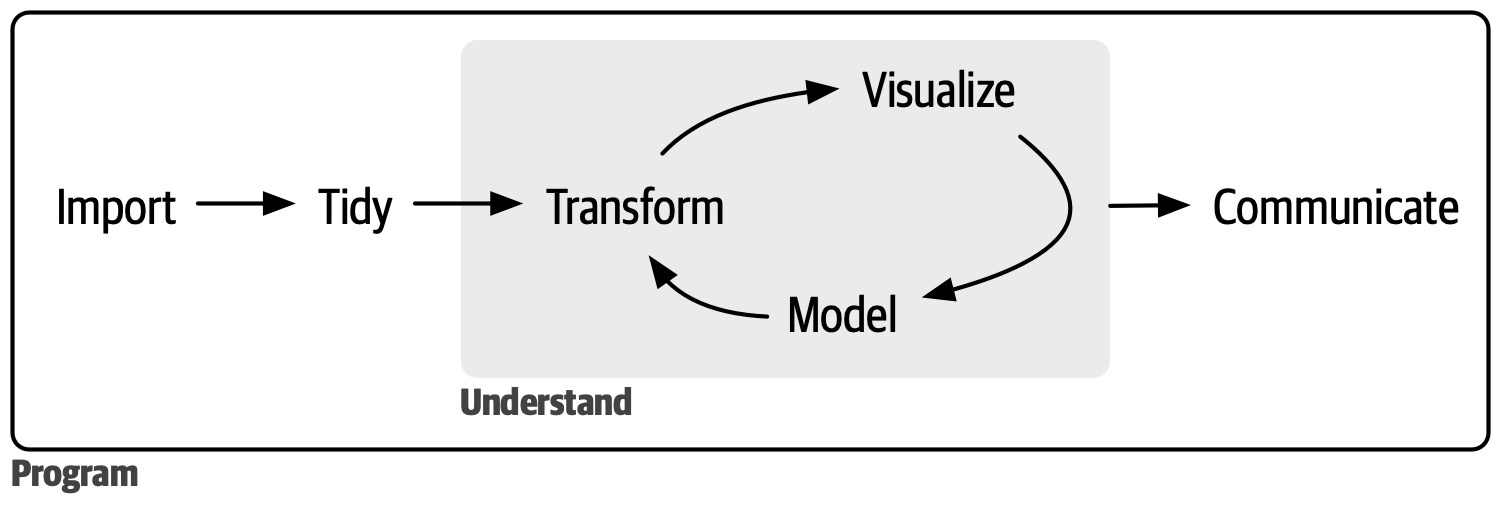
\includegraphics[width=1\linewidth]{./data/base}

\href{https://icu-hsuzuki.github.io/ds4aj/introduction.html\#introduction}{はじめに}に書きましたが、基本的には、問いをもちデータを取得し、視覚化などを通して、データを理解し、さらに問いを深めるサイクルが、データサイエンスの核だと思います。

\begin{quote}
R を使った分析の一つの例を、見て行きます。一つ一つのコード(コンピュータ・プログラム)の簡単な説明は、加えますが、あまりそれに捉われず、「データサイエンスとは何か?」を考えながら、雰囲気を味わってください。
\end{quote}

\hypertarget{r-ux306eux30d1ux30c3ux30b1ux30fcux30b8ux3092ux6d3bux7528}{%
\section{R のパッケージを活用}\label{r-ux306eux30d1ux30c3ux30b1ux30fcux30b8ux3092ux6d3bux7528}}

\hypertarget{ux6e96ux5099-setup}{%
\subsection{準備 Setup}\label{ux6e96ux5099-setup}}

世界銀行(World Bank)の、世界開発指標(WDI: World Development Indicators)の一つの、GDP(Gross Domestic Product 国内総生産)のデータから始めます。GDP にも何種類かの尺度がありますが、次のものを見てみます。

\begin{itemize}
\tightlist
\item
  NY.GDP.MKTP.CD: GDP (current US\$)\footnote{GDP(Gross Domestic Product)とは、ある国のある期間(通常は1年)における、その国で生産されたすべての最終財・サービスの市場価値の総額を指します。これは国内総生産とも呼ばれます。GDPは、その国の経済力や活力を測る指標の1つとして広く用いられています。WDIのGDP (Current USD)は、各国のGDPを米ドルで表したものであり、通貨の価値が異なっても比較可能な形で国際比較ができます。ただし、GDPはあくまで市場価格を基準としているため、非市場活動や自然災害などの影響を受ける場合がある点に注意が必要です。}
\end{itemize}

NY.GDP.MKTP.CD は、データコードと言われるもので、世界開発指標(WDI)には、一つづつ決まっています。

\href{https://datatopics.worldbank.org/world-development-indicators/}{World Development Indicators} のサイトの下にある、Data Themes(テーマ)からテーマを選択し、下にスクロールすると、Code をみることができます。ちなみに、ここで利用する NY.GDP.MKTP.CD: GDP (current US\$) は、テーマ Economy(経済)の、一番上にあります。

経済用語の英語はよく知らないという方は、ブラウザー(Edge, Google Chrome, Safari など)の翻訳機能を使うのも良いでしょう。ただ、そのページの対話型の機能(interactive function)を利用するときは、翻訳機能をOFF にする必要がある場合もありますので、注意してください。

エラーメッセージを調べるときなどに、英語のほうが情報がたくさん得られますから、言語を、英語に変更しておきます。

R には、WDI のデータを取得する R のツール(パッケージ)\texttt{WDI} がありますから、それを使います。また、データを取り扱うための基本的なツール(パッケージ)\texttt{tidyverse} を使いますので、次のコードで、これらを読み込みます。\texttt{\#} 以下はコメント(簡単な説明を書きました) \texttt{\#\textgreater{}} 以下は、コードを実行すると、表示される情報(出力)です。以下同様です。

\begin{Shaded}
\begin{Highlighting}[]
\FunctionTok{Sys.setenv}\NormalTok{(}\AttributeTok{LANG =} \StringTok{"en"}\NormalTok{) }\CommentTok{\# 言語を英語に}
\FunctionTok{library}\NormalTok{(tidyverse)      }\CommentTok{\# tidyverse パッケージを読み込みます}
\CommentTok{\#\textgreater{} {-}{-} Attaching core tidyverse packages {-}{-}{-}{-} tidyverse 2.0.0 {-}{-}}
\CommentTok{\#\textgreater{} v dplyr     1.1.2     v readr     2.1.4}
\CommentTok{\#\textgreater{} v forcats   1.0.0     v stringr   1.5.0}
\CommentTok{\#\textgreater{} v ggplot2   3.4.3     v tibble    3.2.1}
\CommentTok{\#\textgreater{} v lubridate 1.9.2     v tidyr     1.3.0}
\CommentTok{\#\textgreater{} v purrr     1.0.2     }
\CommentTok{\#\textgreater{} {-}{-} Conflicts {-}{-}{-}{-}{-}{-}{-}{-}{-}{-}{-}{-}{-}{-}{-}{-}{-}{-}{-}{-}{-}{-} tidyverse\_conflicts() {-}{-}}
\CommentTok{\#\textgreater{} x dplyr::filter() masks stats::filter()}
\CommentTok{\#\textgreater{} x dplyr::lag()    masks stats::lag()}
\CommentTok{\#\textgreater{} i Use the conflicted package (\textless{}http://conflicted.r{-}lib.org/\textgreater{}) to force all conflicts to become errors}
\FunctionTok{library}\NormalTok{(WDI)            }\CommentTok{\# WDI パッケージを読み込みます}
\end{Highlighting}
\end{Shaded}

データを保存する場所を作成しておくことをお勧めします。保存しておくときは、このディレクトリを使います。

\begin{Shaded}
\begin{Highlighting}[]
\FunctionTok{dir.create}\NormalTok{(}\StringTok{"./data"}\NormalTok{)}
\end{Highlighting}
\end{Shaded}

\hypertarget{ux30c7ux30fcux30bfux53d6ux5f97-import-data}{%
\subsection{データ取得 Import data}\label{ux30c7ux30fcux30bfux53d6ux5f97-import-data}}

データを取得します。少し時間がかかります。取得したデータに、\texttt{df\_gdp} などと、わかりやすい名前をつけます。\texttt{df} は \texttt{data\ frame} の略で、R で標準的なデータの形式です。

\begin{Shaded}
\begin{Highlighting}[]
\NormalTok{df\_gdp }\OtherTok{\textless{}{-}} \FunctionTok{WDI}\NormalTok{(}\AttributeTok{country =} \StringTok{"all"}\NormalTok{, }
              \AttributeTok{indicator =} \FunctionTok{c}\NormalTok{(}\AttributeTok{gdp =} \StringTok{"NY.GDP.MKTP.CD"}\NormalTok{), }
              \AttributeTok{extra =} \ConstantTok{TRUE}\NormalTok{)}
\end{Highlighting}
\end{Shaded}

このコードで、全ての国の GDP を取得できます。GDP の値は、\texttt{NY.GDP.MKTP.CD} という名前の列にありますが、覚えやすいように、gdp という名前に変更しておきます。\texttt{extra\ =\ TRUE} とすることによって、それぞれの国についての情報などが追加されます。

\hypertarget{ux30c7ux30fcux30bfux69cbux9020ux306eux78baux8a8d}{%
\subsection{データ構造の確認}\label{ux30c7ux30fcux30bfux69cbux9020ux306eux78baux8a8d}}

最初の数行だけを見るには、\texttt{head(df\_dgp)} とします。

\begin{Shaded}
\begin{Highlighting}[]
\FunctionTok{head}\NormalTok{(df\_gdp)}
\CommentTok{\#\textgreater{} \# A tibble: 6 x 13}
\CommentTok{\#\textgreater{}   country iso2c iso3c  year    gdp status lastupdated region}
\CommentTok{\#\textgreater{}   \textless{}chr\textgreater{}   \textless{}chr\textgreater{} \textless{}chr\textgreater{} \textless{}dbl\textgreater{}  \textless{}dbl\textgreater{} \textless{}lgl\textgreater{}  \textless{}date\textgreater{}      \textless{}chr\textgreater{} }
\CommentTok{\#\textgreater{} 1 Afghan\textasciitilde{} AF    AFG    1963 7.51e8 NA     2023{-}07{-}25  South\textasciitilde{}}
\CommentTok{\#\textgreater{} 2 Afghan\textasciitilde{} AF    AFG    1962 5.47e8 NA     2023{-}07{-}25  South\textasciitilde{}}
\CommentTok{\#\textgreater{} 3 Afghan\textasciitilde{} AF    AFG    1961 5.49e8 NA     2023{-}07{-}25  South\textasciitilde{}}
\CommentTok{\#\textgreater{} 4 Afghan\textasciitilde{} AF    AFG    1960 5.38e8 NA     2023{-}07{-}25  South\textasciitilde{}}
\CommentTok{\#\textgreater{} 5 Afghan\textasciitilde{} AF    AFG    2003 4.54e9 NA     2023{-}07{-}25  South\textasciitilde{}}
\CommentTok{\#\textgreater{} 6 Afghan\textasciitilde{} AF    AFG    2002 3.85e9 NA     2023{-}07{-}25  South\textasciitilde{}}
\CommentTok{\#\textgreater{} \# i 5 more variables: capital \textless{}chr\textgreater{}, longitude \textless{}dbl\textgreater{},}
\CommentTok{\#\textgreater{} \#   latitude \textless{}dbl\textgreater{}, income \textless{}chr\textgreater{}, lending \textless{}chr\textgreater{}}
\end{Highlighting}
\end{Shaded}

データの構造を見るときには、\texttt{str(df\_gdp)} もよく使われます。今度は、列が縦に並んで表示されます。

\begin{Shaded}
\begin{Highlighting}[]
\FunctionTok{str}\NormalTok{(df\_gdp)}
\CommentTok{\#\textgreater{} spc\_tbl\_ [16,758 x 13] (S3: spec\_tbl\_df/tbl\_df/tbl/data.frame)}
\CommentTok{\#\textgreater{}  $ country    : chr [1:16758] "Afghanistan" "Afghanistan" "Afghanistan" "Afghanistan" ...}
\CommentTok{\#\textgreater{}  $ iso2c      : chr [1:16758] "AF" "AF" "AF" "AF" ...}
\CommentTok{\#\textgreater{}  $ iso3c      : chr [1:16758] "AFG" "AFG" "AFG" "AFG" ...}
\CommentTok{\#\textgreater{}  $ year       : num [1:16758] 1963 1962 1961 1960 2003 ...}
\CommentTok{\#\textgreater{}  $ gdp        : num [1:16758] 7.51e+08 5.47e+08 5.49e+08 5.38e+08 4.54e+09 ...}
\CommentTok{\#\textgreater{}  $ status     : logi [1:16758] NA NA NA NA NA NA ...}
\CommentTok{\#\textgreater{}  $ lastupdated: Date[1:16758], format: "2023{-}07{-}25" ...}
\CommentTok{\#\textgreater{}  $ region     : chr [1:16758] "South Asia" "South Asia" "South Asia" "South Asia" ...}
\CommentTok{\#\textgreater{}  $ capital    : chr [1:16758] "Kabul" "Kabul" "Kabul" "Kabul" ...}
\CommentTok{\#\textgreater{}  $ longitude  : num [1:16758] 69.2 69.2 69.2 69.2 69.2 ...}
\CommentTok{\#\textgreater{}  $ latitude   : num [1:16758] 34.5 34.5 34.5 34.5 34.5 ...}
\CommentTok{\#\textgreater{}  $ income     : chr [1:16758] "Low income" "Low income" "Low income" "Low income" ...}
\CommentTok{\#\textgreater{}  $ lending    : chr [1:16758] "IDA" "IDA" "IDA" "IDA" ...}
\CommentTok{\#\textgreater{}  {-} attr(*, "spec")=}
\CommentTok{\#\textgreater{}   .. cols(}
\CommentTok{\#\textgreater{}   ..   country = col\_character(),}
\CommentTok{\#\textgreater{}   ..   iso2c = col\_character(),}
\CommentTok{\#\textgreater{}   ..   iso3c = col\_character(),}
\CommentTok{\#\textgreater{}   ..   year = col\_double(),}
\CommentTok{\#\textgreater{}   ..   gdp = col\_double(),}
\CommentTok{\#\textgreater{}   ..   status = col\_logical(),}
\CommentTok{\#\textgreater{}   ..   lastupdated = col\_date(format = ""),}
\CommentTok{\#\textgreater{}   ..   region = col\_character(),}
\CommentTok{\#\textgreater{}   ..   capital = col\_character(),}
\CommentTok{\#\textgreater{}   ..   longitude = col\_double(),}
\CommentTok{\#\textgreater{}   ..   latitude = col\_double(),}
\CommentTok{\#\textgreater{}   ..   income = col\_character(),}
\CommentTok{\#\textgreater{}   ..   lending = col\_character()}
\CommentTok{\#\textgreater{}   .. )}
\CommentTok{\#\textgreater{}  {-} attr(*, "problems")=\textless{}externalptr\textgreater{}}
\end{Highlighting}
\end{Shaded}

概要 (\texttt{summary(df\_gdp)}) からもある程度わかります。

\begin{Shaded}
\begin{Highlighting}[]
\FunctionTok{summary}\NormalTok{(df\_gdp) }
\CommentTok{\#\textgreater{}    country             iso2c              iso3c          }
\CommentTok{\#\textgreater{}  Length:16758       Length:16758       Length:16758      }
\CommentTok{\#\textgreater{}  Class :character   Class :character   Class :character  }
\CommentTok{\#\textgreater{}  Mode  :character   Mode  :character   Mode  :character  }
\CommentTok{\#\textgreater{}                                                          }
\CommentTok{\#\textgreater{}                                                          }
\CommentTok{\#\textgreater{}                                                          }
\CommentTok{\#\textgreater{}                                                          }
\CommentTok{\#\textgreater{}       year           gdp             status       }
\CommentTok{\#\textgreater{}  Min.   :1960   Min.   :8.825e+06   Mode:logical  }
\CommentTok{\#\textgreater{}  1st Qu.:1975   1st Qu.:2.523e+09   NA\textquotesingle{}s:16758    }
\CommentTok{\#\textgreater{}  Median :1991   Median :1.843e+10                 }
\CommentTok{\#\textgreater{}  Mean   :1991   Mean   :1.207e+12                 }
\CommentTok{\#\textgreater{}  3rd Qu.:2007   3rd Qu.:2.244e+11                 }
\CommentTok{\#\textgreater{}  Max.   :2022   Max.   :1.006e+14                 }
\CommentTok{\#\textgreater{}                 NA\textquotesingle{}s   :3393                      }
\CommentTok{\#\textgreater{}   lastupdated            region            capital         }
\CommentTok{\#\textgreater{}  Min.   :2023{-}07{-}25   Length:16758       Length:16758      }
\CommentTok{\#\textgreater{}  1st Qu.:2023{-}07{-}25   Class :character   Class :character  }
\CommentTok{\#\textgreater{}  Median :2023{-}07{-}25   Mode  :character   Mode  :character  }
\CommentTok{\#\textgreater{}  Mean   :2023{-}07{-}25                                        }
\CommentTok{\#\textgreater{}  3rd Qu.:2023{-}07{-}25                                        }
\CommentTok{\#\textgreater{}  Max.   :2023{-}07{-}25                                        }
\CommentTok{\#\textgreater{}                                                            }
\CommentTok{\#\textgreater{}    longitude          latitude          income         }
\CommentTok{\#\textgreater{}  Min.   :{-}175.22   Min.   :{-}41.286   Length:16758      }
\CommentTok{\#\textgreater{}  1st Qu.: {-}15.18   1st Qu.:  4.174   Class :character  }
\CommentTok{\#\textgreater{}  Median :  19.54   Median : 17.277   Mode  :character  }
\CommentTok{\#\textgreater{}  Mean   :  19.16   Mean   : 18.740                     }
\CommentTok{\#\textgreater{}  3rd Qu.:  50.53   3rd Qu.: 39.715                     }
\CommentTok{\#\textgreater{}  Max.   : 179.09   Max.   : 64.184                     }
\CommentTok{\#\textgreater{}  NA\textquotesingle{}s   :3528      NA\textquotesingle{}s   :3528                        }
\CommentTok{\#\textgreater{}    lending         }
\CommentTok{\#\textgreater{}  Length:16758      }
\CommentTok{\#\textgreater{}  Class :character  }
\CommentTok{\#\textgreater{}  Mode  :character  }
\CommentTok{\#\textgreater{}                    }
\CommentTok{\#\textgreater{}                    }
\CommentTok{\#\textgreater{}                    }
\CommentTok{\#\textgreater{} }
\end{Highlighting}
\end{Shaded}

国のリストをみてみましょう。とても長いリストの中には、地域名も含まれています。

\begin{Shaded}
\begin{Highlighting}[]
\NormalTok{df\_gdp }\SpecialCharTok{|\textgreater{}} \FunctionTok{distinct}\NormalTok{(country) }\SpecialCharTok{|\textgreater{}} \FunctionTok{pull}\NormalTok{()}
\CommentTok{\#\textgreater{}   [1] "Afghanistan"                                         }
\CommentTok{\#\textgreater{}   [2] "Africa Eastern and Southern"                         }
\CommentTok{\#\textgreater{}   [3] "Africa Western and Central"                          }
\CommentTok{\#\textgreater{}   [4] "Albania"                                             }
\CommentTok{\#\textgreater{}   [5] "Algeria"                                             }
\CommentTok{\#\textgreater{}   [6] "American Samoa"                                      }
\CommentTok{\#\textgreater{}   [7] "Andorra"                                             }
\CommentTok{\#\textgreater{}   [8] "Angola"                                              }
\CommentTok{\#\textgreater{}   [9] "Antigua and Barbuda"                                 }
\CommentTok{\#\textgreater{}  [10] "Arab World"                                          }
\CommentTok{\#\textgreater{}  [11] "Argentina"                                           }
\CommentTok{\#\textgreater{}  [12] "Armenia"                                             }
\CommentTok{\#\textgreater{}  [13] "Aruba"                                               }
\CommentTok{\#\textgreater{}  [14] "Australia"                                           }
\CommentTok{\#\textgreater{}  [15] "Austria"                                             }
\CommentTok{\#\textgreater{}  [16] "Azerbaijan"                                          }
\CommentTok{\#\textgreater{}  [17] "Bahamas, The"                                        }
\CommentTok{\#\textgreater{}  [18] "Bahrain"                                             }
\CommentTok{\#\textgreater{}  [19] "Bangladesh"                                          }
\CommentTok{\#\textgreater{}  [20] "Barbados"                                            }
\CommentTok{\#\textgreater{}  [21] "Belarus"                                             }
\CommentTok{\#\textgreater{}  [22] "Belgium"                                             }
\CommentTok{\#\textgreater{}  [23] "Belize"                                              }
\CommentTok{\#\textgreater{}  [24] "Benin"                                               }
\CommentTok{\#\textgreater{}  [25] "Bermuda"                                             }
\CommentTok{\#\textgreater{}  [26] "Bhutan"                                              }
\CommentTok{\#\textgreater{}  [27] "Bolivia"                                             }
\CommentTok{\#\textgreater{}  [28] "Bosnia and Herzegovina"                              }
\CommentTok{\#\textgreater{}  [29] "Botswana"                                            }
\CommentTok{\#\textgreater{}  [30] "Brazil"                                              }
\CommentTok{\#\textgreater{}  [31] "British Virgin Islands"                              }
\CommentTok{\#\textgreater{}  [32] "Brunei Darussalam"                                   }
\CommentTok{\#\textgreater{}  [33] "Bulgaria"                                            }
\CommentTok{\#\textgreater{}  [34] "Burkina Faso"                                        }
\CommentTok{\#\textgreater{}  [35] "Burundi"                                             }
\CommentTok{\#\textgreater{}  [36] "Cabo Verde"                                          }
\CommentTok{\#\textgreater{}  [37] "Cambodia"                                            }
\CommentTok{\#\textgreater{}  [38] "Cameroon"                                            }
\CommentTok{\#\textgreater{}  [39] "Canada"                                              }
\CommentTok{\#\textgreater{}  [40] "Caribbean small states"                              }
\CommentTok{\#\textgreater{}  [41] "Cayman Islands"                                      }
\CommentTok{\#\textgreater{}  [42] "Central African Republic"                            }
\CommentTok{\#\textgreater{}  [43] "Central Europe and the Baltics"                      }
\CommentTok{\#\textgreater{}  [44] "Chad"                                                }
\CommentTok{\#\textgreater{}  [45] "Channel Islands"                                     }
\CommentTok{\#\textgreater{}  [46] "Chile"                                               }
\CommentTok{\#\textgreater{}  [47] "China"                                               }
\CommentTok{\#\textgreater{}  [48] "Colombia"                                            }
\CommentTok{\#\textgreater{}  [49] "Comoros"                                             }
\CommentTok{\#\textgreater{}  [50] "Congo, Dem. Rep."                                    }
\CommentTok{\#\textgreater{}  [51] "Congo, Rep."                                         }
\CommentTok{\#\textgreater{}  [52] "Costa Rica"                                          }
\CommentTok{\#\textgreater{}  [53] "Cote d\textquotesingle{}Ivoire"                                       }
\CommentTok{\#\textgreater{}  [54] "Croatia"                                             }
\CommentTok{\#\textgreater{}  [55] "Cuba"                                                }
\CommentTok{\#\textgreater{}  [56] "Curacao"                                             }
\CommentTok{\#\textgreater{}  [57] "Cyprus"                                              }
\CommentTok{\#\textgreater{}  [58] "Czechia"                                             }
\CommentTok{\#\textgreater{}  [59] "Denmark"                                             }
\CommentTok{\#\textgreater{}  [60] "Djibouti"                                            }
\CommentTok{\#\textgreater{}  [61] "Dominica"                                            }
\CommentTok{\#\textgreater{}  [62] "Dominican Republic"                                  }
\CommentTok{\#\textgreater{}  [63] "Early{-}demographic dividend"                          }
\CommentTok{\#\textgreater{}  [64] "East Asia \& Pacific"                                 }
\CommentTok{\#\textgreater{}  [65] "East Asia \& Pacific (excluding high income)"         }
\CommentTok{\#\textgreater{}  [66] "East Asia \& Pacific (IDA \& IBRD countries)"          }
\CommentTok{\#\textgreater{}  [67] "Ecuador"                                             }
\CommentTok{\#\textgreater{}  [68] "Egypt, Arab Rep."                                    }
\CommentTok{\#\textgreater{}  [69] "El Salvador"                                         }
\CommentTok{\#\textgreater{}  [70] "Equatorial Guinea"                                   }
\CommentTok{\#\textgreater{}  [71] "Eritrea"                                             }
\CommentTok{\#\textgreater{}  [72] "Estonia"                                             }
\CommentTok{\#\textgreater{}  [73] "Eswatini"                                            }
\CommentTok{\#\textgreater{}  [74] "Ethiopia"                                            }
\CommentTok{\#\textgreater{}  [75] "Euro area"                                           }
\CommentTok{\#\textgreater{}  [76] "Europe \& Central Asia"                               }
\CommentTok{\#\textgreater{}  [77] "Europe \& Central Asia (excluding high income)"       }
\CommentTok{\#\textgreater{}  [78] "Europe \& Central Asia (IDA \& IBRD countries)"        }
\CommentTok{\#\textgreater{}  [79] "European Union"                                      }
\CommentTok{\#\textgreater{}  [80] "Faroe Islands"                                       }
\CommentTok{\#\textgreater{}  [81] "Fiji"                                                }
\CommentTok{\#\textgreater{}  [82] "Finland"                                             }
\CommentTok{\#\textgreater{}  [83] "Fragile and conflict affected situations"            }
\CommentTok{\#\textgreater{}  [84] "France"                                              }
\CommentTok{\#\textgreater{}  [85] "French Polynesia"                                    }
\CommentTok{\#\textgreater{}  [86] "Gabon"                                               }
\CommentTok{\#\textgreater{}  [87] "Gambia, The"                                         }
\CommentTok{\#\textgreater{}  [88] "Georgia"                                             }
\CommentTok{\#\textgreater{}  [89] "Germany"                                             }
\CommentTok{\#\textgreater{}  [90] "Ghana"                                               }
\CommentTok{\#\textgreater{}  [91] "Gibraltar"                                           }
\CommentTok{\#\textgreater{}  [92] "Greece"                                              }
\CommentTok{\#\textgreater{}  [93] "Greenland"                                           }
\CommentTok{\#\textgreater{}  [94] "Grenada"                                             }
\CommentTok{\#\textgreater{}  [95] "Guam"                                                }
\CommentTok{\#\textgreater{}  [96] "Guatemala"                                           }
\CommentTok{\#\textgreater{}  [97] "Guinea"                                              }
\CommentTok{\#\textgreater{}  [98] "Guinea{-}Bissau"                                       }
\CommentTok{\#\textgreater{}  [99] "Guyana"                                              }
\CommentTok{\#\textgreater{} [100] "Haiti"                                               }
\CommentTok{\#\textgreater{} [101] "Heavily indebted poor countries (HIPC)"              }
\CommentTok{\#\textgreater{} [102] "High income"                                         }
\CommentTok{\#\textgreater{} [103] "Honduras"                                            }
\CommentTok{\#\textgreater{} [104] "Hong Kong SAR, China"                                }
\CommentTok{\#\textgreater{} [105] "Hungary"                                             }
\CommentTok{\#\textgreater{} [106] "IBRD only"                                           }
\CommentTok{\#\textgreater{} [107] "Iceland"                                             }
\CommentTok{\#\textgreater{} [108] "IDA \& IBRD total"                                    }
\CommentTok{\#\textgreater{} [109] "IDA blend"                                           }
\CommentTok{\#\textgreater{} [110] "IDA only"                                            }
\CommentTok{\#\textgreater{} [111] "IDA total"                                           }
\CommentTok{\#\textgreater{} [112] "India"                                               }
\CommentTok{\#\textgreater{} [113] "Indonesia"                                           }
\CommentTok{\#\textgreater{} [114] "Iran, Islamic Rep."                                  }
\CommentTok{\#\textgreater{} [115] "Iraq"                                                }
\CommentTok{\#\textgreater{} [116] "Ireland"                                             }
\CommentTok{\#\textgreater{} [117] "Isle of Man"                                         }
\CommentTok{\#\textgreater{} [118] "Israel"                                              }
\CommentTok{\#\textgreater{} [119] "Italy"                                               }
\CommentTok{\#\textgreater{} [120] "Jamaica"                                             }
\CommentTok{\#\textgreater{} [121] "Japan"                                               }
\CommentTok{\#\textgreater{} [122] "Jordan"                                              }
\CommentTok{\#\textgreater{} [123] "Kazakhstan"                                          }
\CommentTok{\#\textgreater{} [124] "Kenya"                                               }
\CommentTok{\#\textgreater{} [125] "Kiribati"                                            }
\CommentTok{\#\textgreater{} [126] "Korea, Dem. People\textquotesingle{}s Rep."                           }
\CommentTok{\#\textgreater{} [127] "Korea, Rep."                                         }
\CommentTok{\#\textgreater{} [128] "Kosovo"                                              }
\CommentTok{\#\textgreater{} [129] "Kuwait"                                              }
\CommentTok{\#\textgreater{} [130] "Kyrgyz Republic"                                     }
\CommentTok{\#\textgreater{} [131] "Lao PDR"                                             }
\CommentTok{\#\textgreater{} [132] "Late{-}demographic dividend"                           }
\CommentTok{\#\textgreater{} [133] "Latin America \& Caribbean"                           }
\CommentTok{\#\textgreater{} [134] "Latin America \& Caribbean (excluding high income)"   }
\CommentTok{\#\textgreater{} [135] "Latin America \& the Caribbean (IDA \& IBRD countries)"}
\CommentTok{\#\textgreater{} [136] "Latvia"                                              }
\CommentTok{\#\textgreater{} [137] "Least developed countries: UN classification"        }
\CommentTok{\#\textgreater{} [138] "Lebanon"                                             }
\CommentTok{\#\textgreater{} [139] "Lesotho"                                             }
\CommentTok{\#\textgreater{} [140] "Liberia"                                             }
\CommentTok{\#\textgreater{} [141] "Libya"                                               }
\CommentTok{\#\textgreater{} [142] "Liechtenstein"                                       }
\CommentTok{\#\textgreater{} [143] "Lithuania"                                           }
\CommentTok{\#\textgreater{} [144] "Low \& middle income"                                 }
\CommentTok{\#\textgreater{} [145] "Low income"                                          }
\CommentTok{\#\textgreater{} [146] "Lower middle income"                                 }
\CommentTok{\#\textgreater{} [147] "Luxembourg"                                          }
\CommentTok{\#\textgreater{} [148] "Macao SAR, China"                                    }
\CommentTok{\#\textgreater{} [149] "Madagascar"                                          }
\CommentTok{\#\textgreater{} [150] "Malawi"                                              }
\CommentTok{\#\textgreater{} [151] "Malaysia"                                            }
\CommentTok{\#\textgreater{} [152] "Maldives"                                            }
\CommentTok{\#\textgreater{} [153] "Mali"                                                }
\CommentTok{\#\textgreater{} [154] "Malta"                                               }
\CommentTok{\#\textgreater{} [155] "Marshall Islands"                                    }
\CommentTok{\#\textgreater{} [156] "Mauritania"                                          }
\CommentTok{\#\textgreater{} [157] "Mauritius"                                           }
\CommentTok{\#\textgreater{} [158] "Mexico"                                              }
\CommentTok{\#\textgreater{} [159] "Micronesia, Fed. Sts."                               }
\CommentTok{\#\textgreater{} [160] "Middle East \& North Africa"                          }
\CommentTok{\#\textgreater{} [161] "Middle East \& North Africa (excluding high income)"  }
\CommentTok{\#\textgreater{} [162] "Middle East \& North Africa (IDA \& IBRD countries)"   }
\CommentTok{\#\textgreater{} [163] "Middle income"                                       }
\CommentTok{\#\textgreater{} [164] "Moldova"                                             }
\CommentTok{\#\textgreater{} [165] "Monaco"                                              }
\CommentTok{\#\textgreater{} [166] "Mongolia"                                            }
\CommentTok{\#\textgreater{} [167] "Montenegro"                                          }
\CommentTok{\#\textgreater{} [168] "Morocco"                                             }
\CommentTok{\#\textgreater{} [169] "Mozambique"                                          }
\CommentTok{\#\textgreater{} [170] "Myanmar"                                             }
\CommentTok{\#\textgreater{} [171] "Namibia"                                             }
\CommentTok{\#\textgreater{} [172] "Nauru"                                               }
\CommentTok{\#\textgreater{} [173] "Nepal"                                               }
\CommentTok{\#\textgreater{} [174] "Netherlands"                                         }
\CommentTok{\#\textgreater{} [175] "New Caledonia"                                       }
\CommentTok{\#\textgreater{} [176] "New Zealand"                                         }
\CommentTok{\#\textgreater{} [177] "Nicaragua"                                           }
\CommentTok{\#\textgreater{} [178] "Niger"                                               }
\CommentTok{\#\textgreater{} [179] "Nigeria"                                             }
\CommentTok{\#\textgreater{} [180] "North America"                                       }
\CommentTok{\#\textgreater{} [181] "North Macedonia"                                     }
\CommentTok{\#\textgreater{} [182] "Northern Mariana Islands"                            }
\CommentTok{\#\textgreater{} [183] "Norway"                                              }
\CommentTok{\#\textgreater{} [184] "Not classified"                                      }
\CommentTok{\#\textgreater{} [185] "OECD members"                                        }
\CommentTok{\#\textgreater{} [186] "Oman"                                                }
\CommentTok{\#\textgreater{} [187] "Other small states"                                  }
\CommentTok{\#\textgreater{} [188] "Pacific island small states"                         }
\CommentTok{\#\textgreater{} [189] "Pakistan"                                            }
\CommentTok{\#\textgreater{} [190] "Palau"                                               }
\CommentTok{\#\textgreater{} [191] "Panama"                                              }
\CommentTok{\#\textgreater{} [192] "Papua New Guinea"                                    }
\CommentTok{\#\textgreater{} [193] "Paraguay"                                            }
\CommentTok{\#\textgreater{} [194] "Peru"                                                }
\CommentTok{\#\textgreater{} [195] "Philippines"                                         }
\CommentTok{\#\textgreater{} [196] "Poland"                                              }
\CommentTok{\#\textgreater{} [197] "Portugal"                                            }
\CommentTok{\#\textgreater{} [198] "Post{-}demographic dividend"                           }
\CommentTok{\#\textgreater{} [199] "Pre{-}demographic dividend"                            }
\CommentTok{\#\textgreater{} [200] "Puerto Rico"                                         }
\CommentTok{\#\textgreater{} [201] "Qatar"                                               }
\CommentTok{\#\textgreater{} [202] "Romania"                                             }
\CommentTok{\#\textgreater{} [203] "Russian Federation"                                  }
\CommentTok{\#\textgreater{} [204] "Rwanda"                                              }
\CommentTok{\#\textgreater{} [205] "Samoa"                                               }
\CommentTok{\#\textgreater{} [206] "San Marino"                                          }
\CommentTok{\#\textgreater{} [207] "Sao Tome and Principe"                               }
\CommentTok{\#\textgreater{} [208] "Saudi Arabia"                                        }
\CommentTok{\#\textgreater{} [209] "Senegal"                                             }
\CommentTok{\#\textgreater{} [210] "Serbia"                                              }
\CommentTok{\#\textgreater{} [211] "Seychelles"                                          }
\CommentTok{\#\textgreater{} [212] "Sierra Leone"                                        }
\CommentTok{\#\textgreater{} [213] "Singapore"                                           }
\CommentTok{\#\textgreater{} [214] "Sint Maarten (Dutch part)"                           }
\CommentTok{\#\textgreater{} [215] "Slovak Republic"                                     }
\CommentTok{\#\textgreater{} [216] "Slovenia"                                            }
\CommentTok{\#\textgreater{} [217] "Small states"                                        }
\CommentTok{\#\textgreater{} [218] "Solomon Islands"                                     }
\CommentTok{\#\textgreater{} [219] "Somalia"                                             }
\CommentTok{\#\textgreater{} [220] "South Africa"                                        }
\CommentTok{\#\textgreater{} [221] "South Asia"                                          }
\CommentTok{\#\textgreater{} [222] "South Asia (IDA \& IBRD)"                             }
\CommentTok{\#\textgreater{} [223] "South Sudan"                                         }
\CommentTok{\#\textgreater{} [224] "Spain"                                               }
\CommentTok{\#\textgreater{} [225] "Sri Lanka"                                           }
\CommentTok{\#\textgreater{} [226] "St. Kitts and Nevis"                                 }
\CommentTok{\#\textgreater{} [227] "St. Lucia"                                           }
\CommentTok{\#\textgreater{} [228] "St. Martin (French part)"                            }
\CommentTok{\#\textgreater{} [229] "St. Vincent and the Grenadines"                      }
\CommentTok{\#\textgreater{} [230] "Sub{-}Saharan Africa"                                  }
\CommentTok{\#\textgreater{} [231] "Sub{-}Saharan Africa (excluding high income)"          }
\CommentTok{\#\textgreater{} [232] "Sub{-}Saharan Africa (IDA \& IBRD countries)"           }
\CommentTok{\#\textgreater{} [233] "Sudan"                                               }
\CommentTok{\#\textgreater{} [234] "Suriname"                                            }
\CommentTok{\#\textgreater{} [235] "Sweden"                                              }
\CommentTok{\#\textgreater{} [236] "Switzerland"                                         }
\CommentTok{\#\textgreater{} [237] "Syrian Arab Republic"                                }
\CommentTok{\#\textgreater{} [238] "Tajikistan"                                          }
\CommentTok{\#\textgreater{} [239] "Tanzania"                                            }
\CommentTok{\#\textgreater{} [240] "Thailand"                                            }
\CommentTok{\#\textgreater{} [241] "Timor{-}Leste"                                         }
\CommentTok{\#\textgreater{} [242] "Togo"                                                }
\CommentTok{\#\textgreater{} [243] "Tonga"                                               }
\CommentTok{\#\textgreater{} [244] "Trinidad and Tobago"                                 }
\CommentTok{\#\textgreater{} [245] "Tunisia"                                             }
\CommentTok{\#\textgreater{} [246] "Turkiye"                                             }
\CommentTok{\#\textgreater{} [247] "Turkmenistan"                                        }
\CommentTok{\#\textgreater{} [248] "Turks and Caicos Islands"                            }
\CommentTok{\#\textgreater{} [249] "Tuvalu"                                              }
\CommentTok{\#\textgreater{} [250] "Uganda"                                              }
\CommentTok{\#\textgreater{} [251] "Ukraine"                                             }
\CommentTok{\#\textgreater{} [252] "United Arab Emirates"                                }
\CommentTok{\#\textgreater{} [253] "United Kingdom"                                      }
\CommentTok{\#\textgreater{} [254] "United States"                                       }
\CommentTok{\#\textgreater{} [255] "Upper middle income"                                 }
\CommentTok{\#\textgreater{} [256] "Uruguay"                                             }
\CommentTok{\#\textgreater{} [257] "Uzbekistan"                                          }
\CommentTok{\#\textgreater{} [258] "Vanuatu"                                             }
\CommentTok{\#\textgreater{} [259] "Venezuela, RB"                                       }
\CommentTok{\#\textgreater{} [260] "Vietnam"                                             }
\CommentTok{\#\textgreater{} [261] "Virgin Islands (U.S.)"                               }
\CommentTok{\#\textgreater{} [262] "West Bank and Gaza"                                  }
\CommentTok{\#\textgreater{} [263] "World"                                               }
\CommentTok{\#\textgreater{} [264] "Yemen, Rep."                                         }
\CommentTok{\#\textgreater{} [265] "Zambia"                                              }
\CommentTok{\#\textgreater{} [266] "Zimbabwe"}
\end{Highlighting}
\end{Shaded}

今回は下のように、\texttt{\textbar{}\textgreater{}}(パイプと呼びます) で繋げてコードを書きました。

\begin{verbatim}
df_gdp |> distinct(country) |> pull()
\end{verbatim}

最初は、データ、その中の、異なる国を選択して、書き出してくださいというものです。

これは、

\begin{verbatim}
pull(distinct(df_gdp, country))
\end{verbatim}

と同じです。どんどん、かっこの中に入れ子になって複雑になるので、一つ一つのステップを、順に書いたものが、最初のものになります。

\begin{verbatim}
df_gdp |> head()
df_gdp |> str()
\end{verbatim}

なども可能です。かっこの中に最初に入るものが直前のもの、ここでは、データになっています。

\hypertarget{ux5fc5ux8981ux306bux5fdcux3058ux3066ux6574ux5f62-transform-data}{%
\subsection{必要に応じて整形 Transform data}\label{ux5fc5ux8981ux306bux5fdcux3058ux3066ux6574ux5f62-transform-data}}

変数が多いので、日本の部分だけ \texttt{filter} を使って選択します。country が Japan と一致する場合のみを選択するときは、\texttt{==} を使います。数値ではないので、引用符をつけます。半角を使ってください。

\begin{Shaded}
\begin{Highlighting}[]
\NormalTok{df\_gdp }\SpecialCharTok{|\textgreater{}} \FunctionTok{filter}\NormalTok{(country }\SpecialCharTok{==} \StringTok{"Japan"}\NormalTok{)}
\CommentTok{\#\textgreater{} \# A tibble: 63 x 13}
\CommentTok{\#\textgreater{}    country iso2c iso3c  year     gdp status lastupdated}
\CommentTok{\#\textgreater{}    \textless{}chr\textgreater{}   \textless{}chr\textgreater{} \textless{}chr\textgreater{} \textless{}dbl\textgreater{}   \textless{}dbl\textgreater{} \textless{}lgl\textgreater{}  \textless{}date\textgreater{}     }
\CommentTok{\#\textgreater{}  1 Japan   JP    JPN    2022 4.23e12 NA     2023{-}07{-}25 }
\CommentTok{\#\textgreater{}  2 Japan   JP    JPN    2021 5.01e12 NA     2023{-}07{-}25 }
\CommentTok{\#\textgreater{}  3 Japan   JP    JPN    2020 5.05e12 NA     2023{-}07{-}25 }
\CommentTok{\#\textgreater{}  4 Japan   JP    JPN    2019 5.12e12 NA     2023{-}07{-}25 }
\CommentTok{\#\textgreater{}  5 Japan   JP    JPN    2018 5.04e12 NA     2023{-}07{-}25 }
\CommentTok{\#\textgreater{}  6 Japan   JP    JPN    2017 4.93e12 NA     2023{-}07{-}25 }
\CommentTok{\#\textgreater{}  7 Japan   JP    JPN    2016 5.00e12 NA     2023{-}07{-}25 }
\CommentTok{\#\textgreater{}  8 Japan   JP    JPN    2015 4.44e12 NA     2023{-}07{-}25 }
\CommentTok{\#\textgreater{}  9 Japan   JP    JPN    2014 4.90e12 NA     2023{-}07{-}25 }
\CommentTok{\#\textgreater{} 10 Japan   JP    JPN    2013 5.21e12 NA     2023{-}07{-}25 }
\CommentTok{\#\textgreater{} \# i 53 more rows}
\CommentTok{\#\textgreater{} \# i 6 more variables: region \textless{}chr\textgreater{}, capital \textless{}chr\textgreater{},}
\CommentTok{\#\textgreater{} \#   longitude \textless{}dbl\textgreater{}, latitude \textless{}dbl\textgreater{}, income \textless{}chr\textgreater{},}
\CommentTok{\#\textgreater{} \#   lending \textless{}chr\textgreater{}}
\end{Highlighting}
\end{Shaded}

\begin{Shaded}
\begin{Highlighting}[]
\NormalTok{df\_gdp }\SpecialCharTok{|\textgreater{}} \FunctionTok{filter}\NormalTok{(country }\SpecialCharTok{==} \StringTok{"Japan"}\NormalTok{) }\SpecialCharTok{|\textgreater{}} \FunctionTok{head}\NormalTok{(}\DecValTok{2}\NormalTok{)}
\CommentTok{\#\textgreater{} \# A tibble: 2 x 13}
\CommentTok{\#\textgreater{}   country iso2c iso3c  year     gdp status lastupdated}
\CommentTok{\#\textgreater{}   \textless{}chr\textgreater{}   \textless{}chr\textgreater{} \textless{}chr\textgreater{} \textless{}dbl\textgreater{}   \textless{}dbl\textgreater{} \textless{}lgl\textgreater{}  \textless{}date\textgreater{}     }
\CommentTok{\#\textgreater{} 1 Japan   JP    JPN    2022 4.23e12 NA     2023{-}07{-}25 }
\CommentTok{\#\textgreater{} 2 Japan   JP    JPN    2021 5.01e12 NA     2023{-}07{-}25 }
\CommentTok{\#\textgreater{} \# i 6 more variables: region \textless{}chr\textgreater{}, capital \textless{}chr\textgreater{},}
\CommentTok{\#\textgreater{} \#   longitude \textless{}dbl\textgreater{}, latitude \textless{}dbl\textgreater{}, income \textless{}chr\textgreater{},}
\CommentTok{\#\textgreater{} \#   lending \textless{}chr\textgreater{}}
\end{Highlighting}
\end{Shaded}

2行目の、gdp の、4.940878e+12 (この文書では、幅の都合で、\texttt{4.9e+12} と表示されているかもしれません)は、Scientific notation と言われるもので、 \[4.940878 \times 10^{12} = 4,940,887,800,000\] を意味します。\texttt{e+3} は千(thousand)、\texttt{e+6} は百万(million)、\texttt{e+9} は、10億(billion)、\texttt{e+12} は、兆(trillion)ですから、日本の、2021 年の GDP は、約5兆ドルとなります。

\hypertarget{ux8996ux899aux5316-data-visualization}{%
\subsection{視覚化 data visualization}\label{ux8996ux899aux5316-data-visualization}}

\hypertarget{fig-1.-ux65e5ux672cux306egdp-ux306eux7d4cux5e74ux5909ux5316ux3092ux8868ux3059ux6298ux7ddaux30b0ux30e9ux30d5line-graph}{%
\subsubsection{Fig 1. 日本のGDP の経年変化を表す折線グラフ(line graph)}\label{fig-1.-ux65e5ux672cux306egdp-ux306eux7d4cux5e74ux5909ux5316ux3092ux8868ux3059ux6298ux7ddaux30b0ux30e9ux30d5line-graph}}

\begin{Shaded}
\begin{Highlighting}[]
\NormalTok{df\_gdp }\SpecialCharTok{|\textgreater{}} \FunctionTok{filter}\NormalTok{(country }\SpecialCharTok{==} \StringTok{"Japan"}\NormalTok{) }\SpecialCharTok{|\textgreater{}}
  \FunctionTok{ggplot}\NormalTok{(}\FunctionTok{aes}\NormalTok{(}\AttributeTok{x =}\NormalTok{ year, }\AttributeTok{y =}\NormalTok{ gdp)) }\SpecialCharTok{+} \FunctionTok{geom\_line}\NormalTok{()}
\end{Highlighting}
\end{Shaded}

\includegraphics{03-first-example_files/figure-latex/unnamed-chunk-13-1.pdf}

\begin{verbatim}
df_gdp |> filter(country == "Japan") |>
  ggplot(aes(x = year, y = gdp)) + geom_line()
\end{verbatim}

日本を選択したときに、それに名前をつけた新しいオブジェクトを作り、それを使うこともできますが、名前がどんどん増えるので、パイプを使って、コードを続けて書いていく方法をとっています。

\texttt{ggplot(aes(x\ =\ year,\ y\ =\ gdp))\ +\ geom\_line()}

の部分が、グラフを描く部分で、「x 軸を、year、y 軸を、gdp として、それを、折線グラフで描いてください」というコードです。

Warning: {[}38;5;238mRemoved 1 row containing missing values

などと表示される場合がありますが、それは、値がない(missing または 値が NA, not available)年があることを言っています。データがない年を最初から削除してこくことも可能です。

\hypertarget{ux30c7ux30fcux30bfux306eux7406ux89e3-understand-data}{%
\subsection{データの理解 Understand data}\label{ux30c7ux30fcux30bfux306eux7406ux89e3-understand-data}}

上の折線グラフを使った、視覚化によって見えてくることがいくつもありますね。どんなことがわかりますか。気づいたこと(observation)をあげてみましょう。

コードを描くことではなく、この部分が、データサイエンスの核の部分です。気づいたこと、疑問点を列挙してみましょう。

急激に増加しているとき、増加減少が繰り返している時、全体としては、1995年ごろからはあまり、増加していないように見えることなどがわかりますね。それぞれのピークや、下落は、なにがあったのかも気になりませんか。これは、世界的な傾向なのでしょうか。日本だけでしょうか。他にも似た傾向の国があるのでしょうか。将来はどうなっていくのでしょうか。などなど。

\hypertarget{ux3055ux307eux3056ux307eux306aux8996ux899aux5316}{%
\subsection{さまざまな視覚化}\label{ux3055ux307eux3056ux307eux306aux8996ux899aux5316}}

\hypertarget{fig-2.-ux5404ux5e74ux3054ux3068ux306eux30c7ux30fcux30bfux306eux6570}{%
\subsubsection{Fig 2. 各年ごとのデータの数}\label{fig-2.-ux5404ux5e74ux3054ux3068ux306eux30c7ux30fcux30bfux306eux6570}}

\texttt{summary(df\_gdp)} で、データ自体は、1960年から2022年までのようですが、年によって、どの程度データがあるか、調べてみます。

\begin{Shaded}
\begin{Highlighting}[]
\NormalTok{df\_gdp }\SpecialCharTok{|\textgreater{}} \FunctionTok{drop\_na}\NormalTok{(gdp) }\SpecialCharTok{|\textgreater{}} \FunctionTok{ggplot}\NormalTok{(}\FunctionTok{aes}\NormalTok{(}\AttributeTok{x =}\NormalTok{ year)) }\SpecialCharTok{+} \FunctionTok{geom\_bar}\NormalTok{()}
\end{Highlighting}
\end{Shaded}

\includegraphics{03-first-example_files/figure-latex/unnamed-chunk-14-1.pdf}

\begin{verbatim}
df_gdp |> drop_na(gdp) |> ggplot(aes(x = year)) + geom_bar()
\end{verbatim}

棒グラフ(bar graph)を使います。\texttt{gdp} の値が、欠損値(NA: not available)のデータを削除してから、グラフを描きます。

\hypertarget{ux5e74ux306egdpux306eux964dux9806ux3067ux306eux8868ux793auxff11}{%
\subsubsection{2022年のGDPの降順での表示(1)}\label{ux5e74ux306egdpux306eux964dux9806ux3067ux306eux8868ux793auxff11}}

最新の2022年のデータはすべてあるわけではなさそうですが、\texttt{gdp} の値が大きい順に並べてみましょう。

\begin{Shaded}
\begin{Highlighting}[]
\NormalTok{df\_gdp }\SpecialCharTok{|\textgreater{}} \FunctionTok{filter}\NormalTok{(year }\SpecialCharTok{==} \DecValTok{2022}\NormalTok{) }\SpecialCharTok{|\textgreater{}} \FunctionTok{drop\_na}\NormalTok{(gdp) }\SpecialCharTok{|\textgreater{}} \FunctionTok{arrange}\NormalTok{(}\FunctionTok{desc}\NormalTok{(gdp))}
\CommentTok{\#\textgreater{} \# A tibble: 233 x 13}
\CommentTok{\#\textgreater{}    country      iso2c iso3c  year     gdp status lastupdated}
\CommentTok{\#\textgreater{}    \textless{}chr\textgreater{}        \textless{}chr\textgreater{} \textless{}chr\textgreater{} \textless{}dbl\textgreater{}   \textless{}dbl\textgreater{} \textless{}lgl\textgreater{}  \textless{}date\textgreater{}     }
\CommentTok{\#\textgreater{}  1 World        1W    WLD    2022 1.01e14 NA     2023{-}07{-}25 }
\CommentTok{\#\textgreater{}  2 High income  XD    \textless{}NA\textgreater{}   2022 6.15e13 NA     2023{-}07{-}25 }
\CommentTok{\#\textgreater{}  3 OECD members OE    OED    2022 5.96e13 NA     2023{-}07{-}25 }
\CommentTok{\#\textgreater{}  4 Post{-}demogr\textasciitilde{} V4    PST    2022 5.60e13 NA     2023{-}07{-}25 }
\CommentTok{\#\textgreater{}  5 IDA \& IBRD \textasciitilde{} ZT    IBT    2022 4.04e13 NA     2023{-}07{-}25 }
\CommentTok{\#\textgreater{}  6 Low \& middl\textasciitilde{} XO    LMY    2022 3.87e13 NA     2023{-}07{-}25 }
\CommentTok{\#\textgreater{}  7 Middle inco\textasciitilde{} XP    MIC    2022 3.82e13 NA     2023{-}07{-}25 }
\CommentTok{\#\textgreater{}  8 IBRD only    XF    IBD    2022 3.76e13 NA     2023{-}07{-}25 }
\CommentTok{\#\textgreater{}  9 East Asia \&\textasciitilde{} Z4    EAS    2022 3.07e13 NA     2023{-}07{-}25 }
\CommentTok{\#\textgreater{} 10 Upper middl\textasciitilde{} XT    \textless{}NA\textgreater{}   2022 3.01e13 NA     2023{-}07{-}25 }
\CommentTok{\#\textgreater{} \# i 223 more rows}
\CommentTok{\#\textgreater{} \# i 6 more variables: region \textless{}chr\textgreater{}, capital \textless{}chr\textgreater{},}
\CommentTok{\#\textgreater{} \#   longitude \textless{}dbl\textgreater{}, latitude \textless{}dbl\textgreater{}, income \textless{}chr\textgreater{},}
\CommentTok{\#\textgreater{} \#   lending \textless{}chr\textgreater{}}
\end{Highlighting}
\end{Shaded}

\hypertarget{ux5e74ux306egdpux306eux964dux9806ux3067ux306eux8868ux793auxff12}{%
\subsubsection{2021年のGDPの降順での表示(2)}\label{ux5e74ux306egdpux306eux964dux9806ux3067ux306eux8868ux793auxff12}}

最初に、World と表示され、グループや、カテゴリーのデータもあるようですから、それを、まず、削除することが必要です。\texttt{region} の列を見ると、World などは、Aggregates となっているので、そのようなものを削除すればよさそうです。数値の大きい順に並べたいので、\texttt{desc} 降順(descending order)にします。

\begin{Shaded}
\begin{Highlighting}[]
\NormalTok{df\_gdp }\SpecialCharTok{|\textgreater{}} \FunctionTok{filter}\NormalTok{(year }\SpecialCharTok{==} \DecValTok{2022}\NormalTok{, region }\SpecialCharTok{!=} \StringTok{"Aggregates"}\NormalTok{) }\SpecialCharTok{|\textgreater{}} 
  \FunctionTok{drop\_na}\NormalTok{(gdp) }\SpecialCharTok{|\textgreater{}} \FunctionTok{arrange}\NormalTok{(}\FunctionTok{desc}\NormalTok{(gdp))}
\CommentTok{\#\textgreater{} \# A tibble: 184 x 13}
\CommentTok{\#\textgreater{}    country      iso2c iso3c  year     gdp status lastupdated}
\CommentTok{\#\textgreater{}    \textless{}chr\textgreater{}        \textless{}chr\textgreater{} \textless{}chr\textgreater{} \textless{}dbl\textgreater{}   \textless{}dbl\textgreater{} \textless{}lgl\textgreater{}  \textless{}date\textgreater{}     }
\CommentTok{\#\textgreater{}  1 United Stat\textasciitilde{} US    USA    2022 2.55e13 NA     2023{-}07{-}25 }
\CommentTok{\#\textgreater{}  2 China        CN    CHN    2022 1.80e13 NA     2023{-}07{-}25 }
\CommentTok{\#\textgreater{}  3 Japan        JP    JPN    2022 4.23e12 NA     2023{-}07{-}25 }
\CommentTok{\#\textgreater{}  4 Germany      DE    DEU    2022 4.07e12 NA     2023{-}07{-}25 }
\CommentTok{\#\textgreater{}  5 India        IN    IND    2022 3.39e12 NA     2023{-}07{-}25 }
\CommentTok{\#\textgreater{}  6 United King\textasciitilde{} GB    GBR    2022 3.07e12 NA     2023{-}07{-}25 }
\CommentTok{\#\textgreater{}  7 France       FR    FRA    2022 2.78e12 NA     2023{-}07{-}25 }
\CommentTok{\#\textgreater{}  8 Russian Fed\textasciitilde{} RU    RUS    2022 2.24e12 NA     2023{-}07{-}25 }
\CommentTok{\#\textgreater{}  9 Canada       CA    CAN    2022 2.14e12 NA     2023{-}07{-}25 }
\CommentTok{\#\textgreater{} 10 Italy        IT    ITA    2022 2.01e12 NA     2023{-}07{-}25 }
\CommentTok{\#\textgreater{} \# i 174 more rows}
\CommentTok{\#\textgreater{} \# i 6 more variables: region \textless{}chr\textgreater{}, capital \textless{}chr\textgreater{},}
\CommentTok{\#\textgreater{} \#   longitude \textless{}dbl\textgreater{}, latitude \textless{}dbl\textgreater{}, income \textless{}chr\textgreater{},}
\CommentTok{\#\textgreater{} \#   lending \textless{}chr\textgreater{}}
\end{Highlighting}
\end{Shaded}

これは、グラフではありませんが、これも一つの可視化と考えられないことはありません。

上位7カ国は、United States, China, Japan, Germany, India, United Kingdom, France であることがわかりました。このあと、Russian Federation, Canada, Italy と続き、でここまでが、2022年のGDP が 2兆ドルを越している国となります。

\hypertarget{fig-3.-2022ux5e74ux6642ux306egdpux4e0aux4f4d7ux30abux56fdux306egdpux7d4cux5e74ux5909ux5316}{%
\subsubsection{Fig 3. 2022年時のGDP上位7カ国のGDP経年変化}\label{fig-3.-2022ux5e74ux6642ux306egdpux4e0aux4f4d7ux30abux56fdux306egdpux7d4cux5e74ux5909ux5316}}

\begin{Shaded}
\begin{Highlighting}[]
\NormalTok{df\_gdp }\SpecialCharTok{|\textgreater{}} \FunctionTok{filter}\NormalTok{(iso2c }\SpecialCharTok{\%in\%} \FunctionTok{c}\NormalTok{(}\StringTok{"US"}\NormalTok{, }\StringTok{"CN"}\NormalTok{, }\StringTok{"JP"}\NormalTok{, }\StringTok{"DE"}\NormalTok{, }\StringTok{"IN"}\NormalTok{, }\StringTok{"GB"}\NormalTok{, }\StringTok{"FR"}\NormalTok{)) }\SpecialCharTok{|\textgreater{}}
  \FunctionTok{ggplot}\NormalTok{(}\FunctionTok{aes}\NormalTok{(}\AttributeTok{x =}\NormalTok{ year, }\AttributeTok{y =}\NormalTok{ gdp, }\AttributeTok{col =}\NormalTok{ iso2c)) }\SpecialCharTok{+} \FunctionTok{geom\_line}\NormalTok{()}
\CommentTok{\#\textgreater{} Warning: Removed 10 rows containing missing values}
\CommentTok{\#\textgreater{} (\textasciigrave{}geom\_line()\textasciigrave{}).}
\end{Highlighting}
\end{Shaded}

\includegraphics{03-first-example_files/figure-latex/unnamed-chunk-17-1.pdf}

\begin{verbatim}
df_gdp |> filter(iso2c %in% c("US", "CN", "JP", "DE", "IN", "GB", "FR")) |>
  ggplot(aes(x = year, y = gdp, col = iso2c)) + geom_line()
\end{verbatim}

ここでは、最初に、\texttt{filter} を使って、7カ国のデータを選択しています。 そのときには、\texttt{\%in\%} として、国名を、combine するといういみで、\texttt{c()} とひとまとめにします。数字ではなく、文字なので、引用符で囲んでいます。この場合は、single quote でも構いませんが、半角を使ってください。

このグラフからは、どのようなことがわかりますか。気づいたことを書いてみましょう。

もう少し、このようなグラフをみてみたいというような、メモも大切です。

\hypertarget{fig-4.-ux4e16ux754cux306egdp-ux306bux304aux3051ux308bux5272ux5408uxff11}{%
\subsubsection{Fig 4. 世界のGDP における割合(1)}\label{fig-4.-ux4e16ux754cux306egdp-ux306bux304aux3051ux308bux5272ux5408uxff11}}

\begin{Shaded}
\begin{Highlighting}[]
\NormalTok{df\_gdp }\SpecialCharTok{|\textgreater{}} 
  \FunctionTok{filter}\NormalTok{(region }\SpecialCharTok{!=} \StringTok{"Aggregates"}\NormalTok{) }\SpecialCharTok{|\textgreater{}} \FunctionTok{drop\_na}\NormalTok{(gdp) }\SpecialCharTok{|\textgreater{}} 
  \FunctionTok{group\_by}\NormalTok{(year) }\SpecialCharTok{|\textgreater{}} \FunctionTok{mutate}\NormalTok{(}\AttributeTok{gdp\_ratio =}\NormalTok{ gdp}\SpecialCharTok{/}\FunctionTok{sum}\NormalTok{(gdp)) }\SpecialCharTok{|\textgreater{}} \FunctionTok{ungroup}\NormalTok{() }\SpecialCharTok{|\textgreater{}}
  \FunctionTok{filter}\NormalTok{(iso2c }\SpecialCharTok{\%in\%} \FunctionTok{c}\NormalTok{(}\StringTok{"US"}\NormalTok{, }\StringTok{"CN"}\NormalTok{, }\StringTok{"JP"}\NormalTok{, }\StringTok{"DE"}\NormalTok{, }\StringTok{"IN"}\NormalTok{, }\StringTok{"GB"}\NormalTok{, }\StringTok{"FR"}\NormalTok{))  }\SpecialCharTok{|\textgreater{}}
  \FunctionTok{ggplot}\NormalTok{(}\FunctionTok{aes}\NormalTok{(}\AttributeTok{x =}\NormalTok{ year, }\AttributeTok{y =}\NormalTok{ gdp\_ratio, }\AttributeTok{fill =}\NormalTok{ iso2c)) }\SpecialCharTok{+} \FunctionTok{geom\_area}\NormalTok{() }\SpecialCharTok{+}
  \FunctionTok{geom\_line}\NormalTok{(}\AttributeTok{col =} \StringTok{"black"}\NormalTok{, }\AttributeTok{position =} \StringTok{"stack"}\NormalTok{, }\AttributeTok{linewidth =} \FloatTok{0.3}\NormalTok{) }\SpecialCharTok{+} 
  \FunctionTok{scale\_y\_continuous}\NormalTok{(}\AttributeTok{labels =}\NormalTok{ scales}\SpecialCharTok{::}\FunctionTok{percent\_format}\NormalTok{(}\AttributeTok{accuracy =} \DecValTok{1}\NormalTok{))}
\end{Highlighting}
\end{Shaded}

\includegraphics{03-first-example_files/figure-latex/unnamed-chunk-18-1.pdf}

まず、下の部分が新しいですが、ここでは、年毎にグループにして、その上で、新しい \texttt{dgp\_ratio} という名前の列を追加し、その gdp の値を、gdp 合計で割っています。すなわち、世界の、GDP における割合が計算されています。

\begin{verbatim}
  group_by(year) |> mutate(gdp_ratio = gdp/sum(gdp)) |> ungroup() |>
\end{verbatim}

下の部分では、\texttt{geom\_area} を使って、\texttt{fill=iso2c} により、\texttt{iso2c} ごとに、違う色を塗って、position = ``stack'' により、積み上げ型の、グラフを描き、境目がわかりやすいように、0.3 の太さの黒の線を描いてください。また、y 軸は、小数点以下を省いたパーセント表示に変えてください。というコードです。

\begin{verbatim}
  ggplot(aes(x = year, y = gdp_ratio, fill = iso2c)) + geom_area() +
  geom_line(col = "black", position = "stack", linewidth = 0.3) + 
  scale_y_continuous(labels = scales::percent_format(accuracy = 1))
\end{verbatim}

\hypertarget{fig-4.-ux4e16ux754cux306egdp-ux306bux304aux3051ux308bux5272ux5408uxff12}{%
\subsubsection{Fig 4. 世界のGDP における割合(2)}\label{fig-4.-ux4e16ux754cux306egdp-ux306bux304aux3051ux308bux5272ux5408uxff12}}

これは、上から、iso2c の アルファベットの順番になっていますが、積み上げの順序を変更することもできます。

\begin{Shaded}
\begin{Highlighting}[]
\NormalTok{df\_gdp }\SpecialCharTok{|\textgreater{}} 
  \FunctionTok{filter}\NormalTok{(region }\SpecialCharTok{!=} \StringTok{"Aggregates"}\NormalTok{) }\SpecialCharTok{|\textgreater{}} \FunctionTok{drop\_na}\NormalTok{(gdp) }\SpecialCharTok{|\textgreater{}} 
  \FunctionTok{group\_by}\NormalTok{(year) }\SpecialCharTok{|\textgreater{}} \FunctionTok{mutate}\NormalTok{(}\AttributeTok{gdp\_ratio =}\NormalTok{ gdp}\SpecialCharTok{/}\FunctionTok{sum}\NormalTok{(gdp)) }\SpecialCharTok{|\textgreater{}} \FunctionTok{ungroup}\NormalTok{() }\SpecialCharTok{|\textgreater{}}
  \FunctionTok{filter}\NormalTok{(iso2c }\SpecialCharTok{\%in\%} \FunctionTok{c}\NormalTok{(}\StringTok{"US"}\NormalTok{, }\StringTok{"CN"}\NormalTok{, }\StringTok{"JP"}\NormalTok{, }\StringTok{"DE"}\NormalTok{, }\StringTok{"IN"}\NormalTok{, }\StringTok{"GB"}\NormalTok{, }\StringTok{"FR"}\NormalTok{))  }\SpecialCharTok{|\textgreater{}}
  \FunctionTok{mutate}\NormalTok{(}\AttributeTok{iso2co =} \FunctionTok{factor}\NormalTok{(iso2c, }\AttributeTok{levels =} \FunctionTok{c}\NormalTok{(}\StringTok{"IN"}\NormalTok{, }\StringTok{"CN"}\NormalTok{, }\StringTok{"FR"}\NormalTok{, }\StringTok{"GB"}\NormalTok{, }\StringTok{"DE"}\NormalTok{, }\StringTok{"JP"}\NormalTok{, }\StringTok{"US"}\NormalTok{))) }\SpecialCharTok{|\textgreater{}}
  \FunctionTok{ggplot}\NormalTok{(}\FunctionTok{aes}\NormalTok{(}\AttributeTok{x =}\NormalTok{ year, }\AttributeTok{y =}\NormalTok{ gdp\_ratio, }\AttributeTok{fill =}\NormalTok{ iso2co)) }\SpecialCharTok{+} \FunctionTok{geom\_area}\NormalTok{() }\SpecialCharTok{+}
  \FunctionTok{geom\_line}\NormalTok{(}\AttributeTok{col =} \StringTok{"black"}\NormalTok{, }\AttributeTok{position =} \StringTok{"stack"}\NormalTok{, }\AttributeTok{linewidth =} \FloatTok{0.3}\NormalTok{) }\SpecialCharTok{+} 
  \FunctionTok{scale\_y\_continuous}\NormalTok{(}\AttributeTok{labels =}\NormalTok{ scales}\SpecialCharTok{::}\FunctionTok{percent\_format}\NormalTok{(}\AttributeTok{accuracy =} \DecValTok{1}\NormalTok{))}
\end{Highlighting}
\end{Shaded}

\includegraphics{03-first-example_files/figure-latex/unnamed-chunk-19-1.pdf}

これらは、世界全体の GPT における割合です。

どのようなことがわかりますか。

主要国で、60\%〜70\% を占めていることがわかります。それぞれの国や、幾つかの国の影響力や、その時代による変化も、ある程度みることができるように思います。

気づいたこと、疑問に思ったことなどを、書き出してみてください。

GDP が大きな国と、小さな国があるのはわかりますが、それは、どのように分布しているのでしょうか。

\hypertarget{fig-5.-2022ux5e74ux306eux4e16ux754cux306eux56fdux306egdpux306eux5206ux5e03uxff11}{%
\subsubsection{Fig 5. 2022年の世界の国のGDPの分布(1)}\label{fig-5.-2022ux5e74ux306eux4e16ux754cux306eux56fdux306egdpux306eux5206ux5e03uxff11}}

\begin{Shaded}
\begin{Highlighting}[]
\NormalTok{df\_gdp }\SpecialCharTok{|\textgreater{}} \FunctionTok{drop\_na}\NormalTok{(gdp) }\SpecialCharTok{|\textgreater{}} 
  \FunctionTok{filter}\NormalTok{(year }\SpecialCharTok{==} \DecValTok{2022}\NormalTok{) }\SpecialCharTok{|\textgreater{}} \FunctionTok{filter}\NormalTok{(region }\SpecialCharTok{!=} \StringTok{"Aggregates"}\NormalTok{) }\SpecialCharTok{|\textgreater{}}
  \FunctionTok{ggplot}\NormalTok{(}\FunctionTok{aes}\NormalTok{(gdp)) }\SpecialCharTok{+} \FunctionTok{geom\_histogram}\NormalTok{()}
\CommentTok{\#\textgreater{} \textasciigrave{}stat\_bin()\textasciigrave{} using \textasciigrave{}bins = 30\textasciigrave{}. Pick better value with}
\CommentTok{\#\textgreater{} \textasciigrave{}binwidth\textasciigrave{}.}
\end{Highlighting}
\end{Shaded}

\includegraphics{03-first-example_files/figure-latex/unnamed-chunk-20-1.pdf}

小さいところに集中していることがわかりますが、\texttt{scale\_x\_log10()} を加え、対数軸をとってみます。

\(log10(1000) = 3\), \(log10(1000000) = 6\), \(log10(1000000000) = 9\) などになります。

\hypertarget{fig-6.-2022ux5e74ux306eux4e16ux754cux306eux56fdux306egdpux306eux5206ux5e03uxff12}{%
\subsubsection{Fig 6. 2022年の世界の国のGDPの分布(2)}\label{fig-6.-2022ux5e74ux306eux4e16ux754cux306eux56fdux306egdpux306eux5206ux5e03uxff12}}

\begin{Shaded}
\begin{Highlighting}[]
\NormalTok{df\_gdp }\SpecialCharTok{|\textgreater{}} \FunctionTok{drop\_na}\NormalTok{(gdp) }\SpecialCharTok{|\textgreater{}} 
  \FunctionTok{filter}\NormalTok{(year }\SpecialCharTok{==} \DecValTok{2022}\NormalTok{) }\SpecialCharTok{|\textgreater{}} \FunctionTok{filter}\NormalTok{(region }\SpecialCharTok{!=} \StringTok{"Aggregates"}\NormalTok{) }\SpecialCharTok{|\textgreater{}}
  \FunctionTok{ggplot}\NormalTok{(}\FunctionTok{aes}\NormalTok{(gdp)) }\SpecialCharTok{+} \FunctionTok{geom\_histogram}\NormalTok{() }\SpecialCharTok{+} \FunctionTok{scale\_x\_log10}\NormalTok{()}
\CommentTok{\#\textgreater{} \textasciigrave{}stat\_bin()\textasciigrave{} using \textasciigrave{}bins = 30\textasciigrave{}. Pick better value with}
\CommentTok{\#\textgreater{} \textasciigrave{}binwidth\textasciigrave{}.}
\end{Highlighting}
\end{Shaded}

\includegraphics{03-first-example_files/figure-latex/unnamed-chunk-21-1.pdf}

幅を変更したり、分ける個数を変更するには \texttt{binwidth\ =\ 0.5} や、\texttt{bins\ =\ 20} を、\texttt{geom\_histogram()} のかっこの中に入れます。

\hypertarget{fig-7.-2021ux5e74ux306eux4e16ux754cux306eux56fdux306egdpux306eux5206ux5e03uxff13}{%
\subsubsection{Fig 7. 2021年の世界の国のGDPの分布(3)}\label{fig-7.-2021ux5e74ux306eux4e16ux754cux306eux56fdux306egdpux306eux5206ux5e03uxff13}}

また、密度曲線に変えるには、\texttt{geom\_density} を使います。

\begin{Shaded}
\begin{Highlighting}[]
\NormalTok{df\_gdp }\SpecialCharTok{|\textgreater{}} \FunctionTok{drop\_na}\NormalTok{(gdp) }\SpecialCharTok{|\textgreater{}} 
  \FunctionTok{filter}\NormalTok{(year }\SpecialCharTok{==} \DecValTok{2021}\NormalTok{) }\SpecialCharTok{|\textgreater{}} \FunctionTok{filter}\NormalTok{(region }\SpecialCharTok{!=} \StringTok{"Aggregates"}\NormalTok{) }\SpecialCharTok{|\textgreater{}}
  \FunctionTok{ggplot}\NormalTok{(}\FunctionTok{aes}\NormalTok{(gdp)) }\SpecialCharTok{+} \FunctionTok{geom\_density}\NormalTok{() }\SpecialCharTok{+} \FunctionTok{scale\_x\_log10}\NormalTok{()}
\end{Highlighting}
\end{Shaded}

\includegraphics{03-first-example_files/figure-latex/unnamed-chunk-22-1.pdf}

\hypertarget{fig-8.-2022ux5e74ux307eux3067ux306eux4e16ux754cux306eux56fdux306egdpux306eux5206ux5e03uxff14}{%
\subsubsection{Fig 8. 2022年までの世界の国のGDPの分布(4)}\label{fig-8.-2022ux5e74ux307eux3067ux306eux4e16ux754cux306eux56fdux306egdpux306eux5206ux5e03uxff14}}

これは、2022年のデータですが、10年ごとの、density の変化を見てみます。alpha の値は透明度です。

\begin{Shaded}
\begin{Highlighting}[]
\NormalTok{df\_gdp }\SpecialCharTok{|\textgreater{}} \FunctionTok{drop\_na}\NormalTok{(gdp) }\SpecialCharTok{|\textgreater{}} 
  \FunctionTok{filter}\NormalTok{(year }\SpecialCharTok{\%in\%} \FunctionTok{c}\NormalTok{(}\DecValTok{1962}\NormalTok{, }\DecValTok{1972}\NormalTok{, }\DecValTok{1982}\NormalTok{, }\DecValTok{1992}\NormalTok{, }\DecValTok{2002}\NormalTok{, }\DecValTok{2012}\NormalTok{, }\DecValTok{2022}\NormalTok{)) }\SpecialCharTok{|\textgreater{}}
  \FunctionTok{ggplot}\NormalTok{(}\FunctionTok{aes}\NormalTok{(gdp, }\AttributeTok{fill =} \FunctionTok{factor}\NormalTok{(year))) }\SpecialCharTok{+} \FunctionTok{geom\_density}\NormalTok{(}\AttributeTok{alpha =} \FloatTok{0.4}\NormalTok{) }\SpecialCharTok{+} \FunctionTok{scale\_x\_log10}\NormalTok{()}
\end{Highlighting}
\end{Shaded}

\includegraphics{03-first-example_files/figure-latex/unnamed-chunk-23-1.pdf}

\hypertarget{fig-9.-2022ux5e74ux306eux4e16ux754cux306eux56fdux306egdpux306eux5206ux5e03uxff15}{%
\subsubsection{Fig 9. 2022年の世界の国のGDPの分布(5)}\label{fig-9.-2022ux5e74ux306eux4e16ux754cux306eux56fdux306egdpux306eux5206ux5e03uxff15}}

少しみにくいので、分けてみます。

\begin{Shaded}
\begin{Highlighting}[]
\NormalTok{df\_gdp }\SpecialCharTok{|\textgreater{}} \FunctionTok{drop\_na}\NormalTok{(gdp) }\SpecialCharTok{|\textgreater{}} 
  \FunctionTok{filter}\NormalTok{(year }\SpecialCharTok{\%in\%} \FunctionTok{c}\NormalTok{(}\DecValTok{1972}\NormalTok{, }\DecValTok{1982}\NormalTok{, }\DecValTok{1992}\NormalTok{, }\DecValTok{2002}\NormalTok{, }\DecValTok{2012}\NormalTok{, }\DecValTok{2022}\NormalTok{)) }\SpecialCharTok{|\textgreater{}}
  \FunctionTok{ggplot}\NormalTok{(}\FunctionTok{aes}\NormalTok{(gdp, }\AttributeTok{fill =} \FunctionTok{factor}\NormalTok{(year))) }\SpecialCharTok{+} 
  \FunctionTok{geom\_density}\NormalTok{() }\SpecialCharTok{+} \FunctionTok{scale\_x\_log10}\NormalTok{() }\SpecialCharTok{+} \FunctionTok{facet\_wrap}\NormalTok{(}\SpecialCharTok{\textasciitilde{}}\NormalTok{year)}
\end{Highlighting}
\end{Shaded}

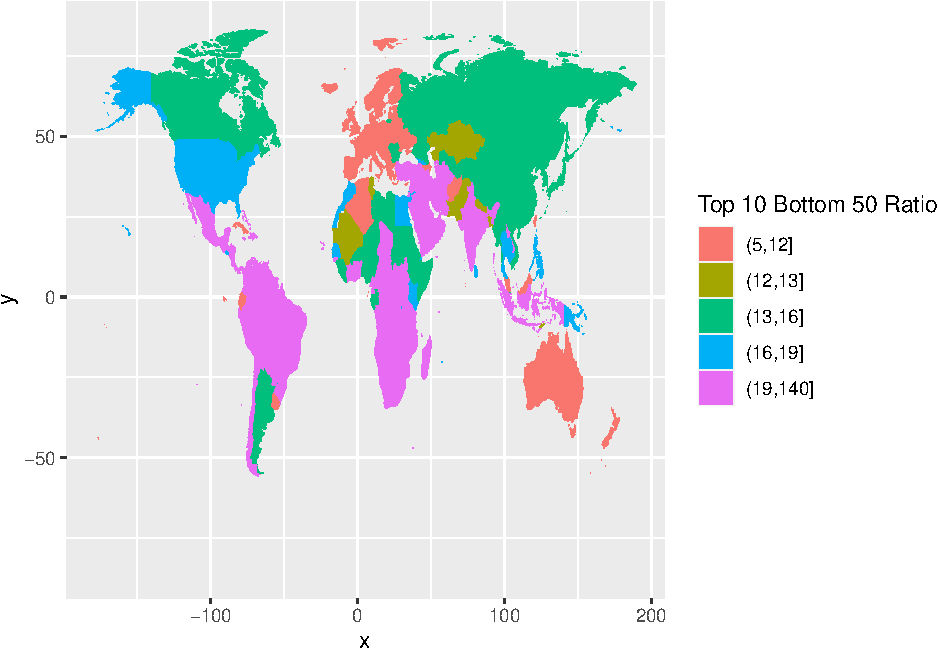
\includegraphics{03-first-example_files/figure-latex/unnamed-chunk-24-1.pdf}

\hypertarget{fig-10.-ux5730ux57dfux3054ux3068ux306e-gdp-ux306eux5206ux5e03}{%
\subsubsection{Fig 10. 地域ごとの GDP の分布}\label{fig-10.-ux5730ux57dfux3054ux3068ux306e-gdp-ux306eux5206ux5e03}}

いくつかのグループごとに分布をみてみることも可能です。それには、箱ひげ図(Boxplot)が有効です。箱ひげ図では、そのグループの国を値の大きさの順にならべて、四等分し、その、真ん中の二つが箱の部分に対応しています。また、真ん中の太い線は、中央値(median)を表しています。詳しくは、後ほど説明します。

\begin{Shaded}
\begin{Highlighting}[]
\NormalTok{df\_gdp }\SpecialCharTok{|\textgreater{}} \FunctionTok{drop\_na}\NormalTok{(gdp) }\SpecialCharTok{|\textgreater{}} \FunctionTok{filter}\NormalTok{(region }\SpecialCharTok{!=} \StringTok{"Aggregates"}\NormalTok{) }\SpecialCharTok{|\textgreater{}}
  \FunctionTok{drop\_na}\NormalTok{(region) }\SpecialCharTok{|\textgreater{}} \FunctionTok{filter}\NormalTok{(year }\SpecialCharTok{\%in\%} \FunctionTok{c}\NormalTok{(}\DecValTok{2022}\NormalTok{)) }\SpecialCharTok{|\textgreater{}}
  \FunctionTok{ggplot}\NormalTok{(}\FunctionTok{aes}\NormalTok{(gdp, region, }\AttributeTok{fill =}\NormalTok{ region)) }\SpecialCharTok{+} 
  \FunctionTok{geom\_boxplot}\NormalTok{() }\SpecialCharTok{+} \FunctionTok{scale\_x\_log10}\NormalTok{() }\SpecialCharTok{+} \FunctionTok{labs}\NormalTok{(}\AttributeTok{y =} \StringTok{""}\NormalTok{) }\SpecialCharTok{+} 
  \FunctionTok{theme}\NormalTok{(}\AttributeTok{legend.position =} \StringTok{"none"}\NormalTok{)}
\end{Highlighting}
\end{Shaded}

\includegraphics{03-first-example_files/figure-latex/unnamed-chunk-25-1.pdf}

\hypertarget{fig-11.-ux53ceux5165ux306eux591aux5be1ux306bux3088ux308bux5206ux985eux3054ux3068ux306e-gdp-ux5206ux5e03}{%
\subsubsection{Fig 11. 収入の多寡による分類ごとの GDP 分布}\label{fig-11.-ux53ceux5165ux306eux591aux5be1ux306bux3088ux308bux5206ux985eux3054ux3068ux306e-gdp-ux5206ux5e03}}

\begin{Shaded}
\begin{Highlighting}[]
\NormalTok{df\_gdp }\SpecialCharTok{|\textgreater{}} \FunctionTok{drop\_na}\NormalTok{(gdp) }\SpecialCharTok{|\textgreater{}} \FunctionTok{filter}\NormalTok{(region }\SpecialCharTok{!=} \StringTok{"Aggregates"}\NormalTok{) }\SpecialCharTok{|\textgreater{}}
  \FunctionTok{drop\_na}\NormalTok{(income) }\SpecialCharTok{|\textgreater{}} \FunctionTok{filter}\NormalTok{(year }\SpecialCharTok{\%in\%} \FunctionTok{c}\NormalTok{(}\DecValTok{2022}\NormalTok{)) }\SpecialCharTok{|\textgreater{}}
  \FunctionTok{mutate}\NormalTok{(}\AttributeTok{level =} \FunctionTok{factor}\NormalTok{(income, }\FunctionTok{c}\NormalTok{(}\StringTok{"High income"}\NormalTok{, }\StringTok{"Upper middle income"}\NormalTok{, }\StringTok{"Lower middle income"}\NormalTok{, }\StringTok{"Low income"}\NormalTok{))) }\SpecialCharTok{|\textgreater{}}
  \FunctionTok{ggplot}\NormalTok{(}\FunctionTok{aes}\NormalTok{(gdp, level, }\AttributeTok{fill =}\NormalTok{ income)) }\SpecialCharTok{+} 
  \FunctionTok{geom\_boxplot}\NormalTok{() }\SpecialCharTok{+} \FunctionTok{scale\_x\_log10}\NormalTok{() }\SpecialCharTok{+} \FunctionTok{labs}\NormalTok{(}\AttributeTok{y =} \StringTok{""}\NormalTok{) }\SpecialCharTok{+} 
  \FunctionTok{theme}\NormalTok{(}\AttributeTok{legend.position =} \StringTok{"none"}\NormalTok{)}
\end{Highlighting}
\end{Shaded}

\includegraphics{03-first-example_files/figure-latex/unnamed-chunk-26-1.pdf}

これからも、いろいろなことがわかりますね。点は、外れ値を表しています。外れ値についても、きちんと決まっています。収入の多寡(Income Level)のグループは、GNI per Capita という、一人当たりの国民総所得(GNI を人口で割ったもの)をもとに、世界銀行が決めているものです。

\hypertarget{ux4e16ux754cux5730ux56f3ux306eux6e96ux5099}{%
\subsubsection{世界地図の準備}\label{ux4e16ux754cux5730ux56f3ux306eux6e96ux5099}}

地図で、国の収入の多寡(income level) をみてみましょう。

\begin{Shaded}
\begin{Highlighting}[]
\FunctionTok{library}\NormalTok{(maps)}
\NormalTok{gdp\_short }\OtherTok{\textless{}{-}}\NormalTok{ df\_gdp }\SpecialCharTok{|\textgreater{}} \FunctionTok{filter}\NormalTok{(year }\SpecialCharTok{==} \DecValTok{2022}\NormalTok{, region }\SpecialCharTok{!=} \StringTok{"Aggregates"}\NormalTok{) }\SpecialCharTok{|\textgreater{}}
  \FunctionTok{select}\NormalTok{(iso2c, gdp, income)}
\NormalTok{map\_world }\OtherTok{\textless{}{-}} \FunctionTok{map\_data}\NormalTok{(}\StringTok{\textquotesingle{}world\textquotesingle{}}\NormalTok{)}
\NormalTok{map\_gdp }\OtherTok{\textless{}{-}}\NormalTok{ map\_world }\SpecialCharTok{|\textgreater{}} 
  \FunctionTok{mutate}\NormalTok{(}\AttributeTok{iso2c =} \FunctionTok{iso.alpha}\NormalTok{(region, }\AttributeTok{n=}\DecValTok{2}\NormalTok{)) }\SpecialCharTok{|\textgreater{}} 
  \FunctionTok{left\_join}\NormalTok{(gdp\_short, }\AttributeTok{by =} \StringTok{"iso2c"}\NormalTok{) }
\FunctionTok{head}\NormalTok{(map\_gdp)}
\CommentTok{\#\textgreater{}        long      lat group order region subregion iso2c gdp}
\CommentTok{\#\textgreater{} 1 {-}69.89912 12.45200     1     1  Aruba      \textless{}NA\textgreater{}    AW  NA}
\CommentTok{\#\textgreater{} 2 {-}69.89571 12.42300     1     2  Aruba      \textless{}NA\textgreater{}    AW  NA}
\CommentTok{\#\textgreater{} 3 {-}69.94219 12.43853     1     3  Aruba      \textless{}NA\textgreater{}    AW  NA}
\CommentTok{\#\textgreater{} 4 {-}70.00415 12.50049     1     4  Aruba      \textless{}NA\textgreater{}    AW  NA}
\CommentTok{\#\textgreater{} 5 {-}70.06612 12.54697     1     5  Aruba      \textless{}NA\textgreater{}    AW  NA}
\CommentTok{\#\textgreater{} 6 {-}70.05088 12.59707     1     6  Aruba      \textless{}NA\textgreater{}    AW  NA}
\CommentTok{\#\textgreater{}        income}
\CommentTok{\#\textgreater{} 1 High income}
\CommentTok{\#\textgreater{} 2 High income}
\CommentTok{\#\textgreater{} 3 High income}
\CommentTok{\#\textgreater{} 4 High income}
\CommentTok{\#\textgreater{} 5 High income}
\CommentTok{\#\textgreater{} 6 High income}
\end{Highlighting}
\end{Shaded}

\hypertarget{fig-12.-income-level-ux306bux3088ux308bux8272ux5206ux3051ux5730ux56f3}{%
\subsubsection{Fig 12. Income Level による色分け地図}\label{fig-12.-income-level-ux306bux3088ux308bux8272ux5206ux3051ux5730ux56f3}}

\begin{Shaded}
\begin{Highlighting}[]
\NormalTok{map\_gdp }\SpecialCharTok{|\textgreater{}} \FunctionTok{mutate}\NormalTok{(}\AttributeTok{income\_level =} \FunctionTok{factor}\NormalTok{(income, }\AttributeTok{levels =} \FunctionTok{c}\NormalTok{(}\StringTok{"High income"}\NormalTok{, }\StringTok{"Upper middle income"}\NormalTok{, }\StringTok{"Lower middle income"}\NormalTok{, }\StringTok{"Low income"}\NormalTok{, }\StringTok{"Not classified"}\NormalTok{, }\ConstantTok{NA}\NormalTok{))) }\SpecialCharTok{|\textgreater{}}
  \FunctionTok{ggplot}\NormalTok{() }\SpecialCharTok{+}
  \FunctionTok{geom\_map}\NormalTok{(}\FunctionTok{aes}\NormalTok{(long, lat, }\AttributeTok{map\_id =}\NormalTok{ region, }\AttributeTok{fill =}\NormalTok{ income\_level), }\AttributeTok{map =}\NormalTok{ map\_world, }\AttributeTok{col =} \StringTok{"black"}\NormalTok{, }\AttributeTok{size =} \FloatTok{0.1}\NormalTok{) }
\CommentTok{\#\textgreater{} Warning: Using \textasciigrave{}size\textasciigrave{} aesthetic for lines was deprecated in ggplot2}
\CommentTok{\#\textgreater{} 3.4.0.}
\CommentTok{\#\textgreater{} i Please use \textasciigrave{}linewidth\textasciigrave{} instead.}
\CommentTok{\#\textgreater{} This warning is displayed once every 8 hours.}
\CommentTok{\#\textgreater{} Call \textasciigrave{}lifecycle::last\_lifecycle\_warnings()\textasciigrave{} to see where}
\CommentTok{\#\textgreater{} this warning was generated.}
\CommentTok{\#\textgreater{} Warning in geom\_map(aes(long, lat, map\_id = region, fill =}
\CommentTok{\#\textgreater{} income\_level), : Ignoring unknown aesthetics: x and y}
\end{Highlighting}
\end{Shaded}

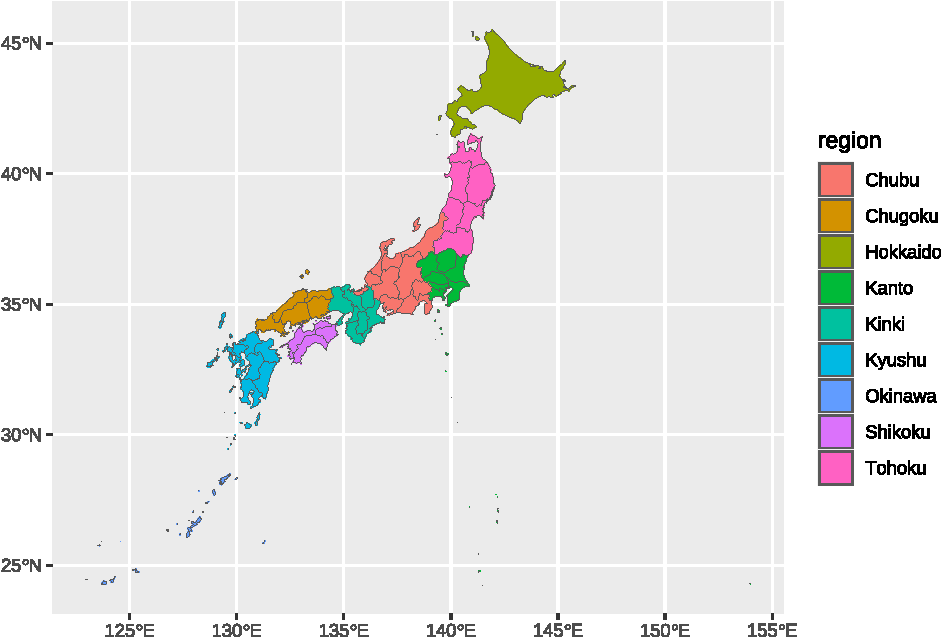
\includegraphics{03-first-example_files/figure-latex/unnamed-chunk-28-1.pdf}

\hypertarget{fig-13.-gdp-ux306bux3088ux308bux8272ux5206ux3051ux5730ux56f3}{%
\subsubsection{Fig 13. GDP による色分け地図}\label{fig-13.-gdp-ux306bux3088ux308bux8272ux5206ux3051ux5730ux56f3}}

\begin{Shaded}
\begin{Highlighting}[]
\NormalTok{map\_gdp }\SpecialCharTok{|\textgreater{}}
  \FunctionTok{ggplot}\NormalTok{() }\SpecialCharTok{+}
  \FunctionTok{geom\_map}\NormalTok{(}\FunctionTok{aes}\NormalTok{(}\AttributeTok{x=}\NormalTok{long, }\AttributeTok{y=}\NormalTok{lat, }\AttributeTok{map\_id =}\NormalTok{ region, }\AttributeTok{fill =}\NormalTok{ gdp), }\AttributeTok{map =}\NormalTok{ map\_world, }\AttributeTok{col =} \StringTok{"black"}\NormalTok{, }\AttributeTok{size =} \FloatTok{0.1}\NormalTok{) }
\CommentTok{\#\textgreater{} Warning in geom\_map(aes(x = long, y = lat, map\_id = region,}
\CommentTok{\#\textgreater{} fill = gdp), : Ignoring unknown aesthetics: x and y}
\end{Highlighting}
\end{Shaded}

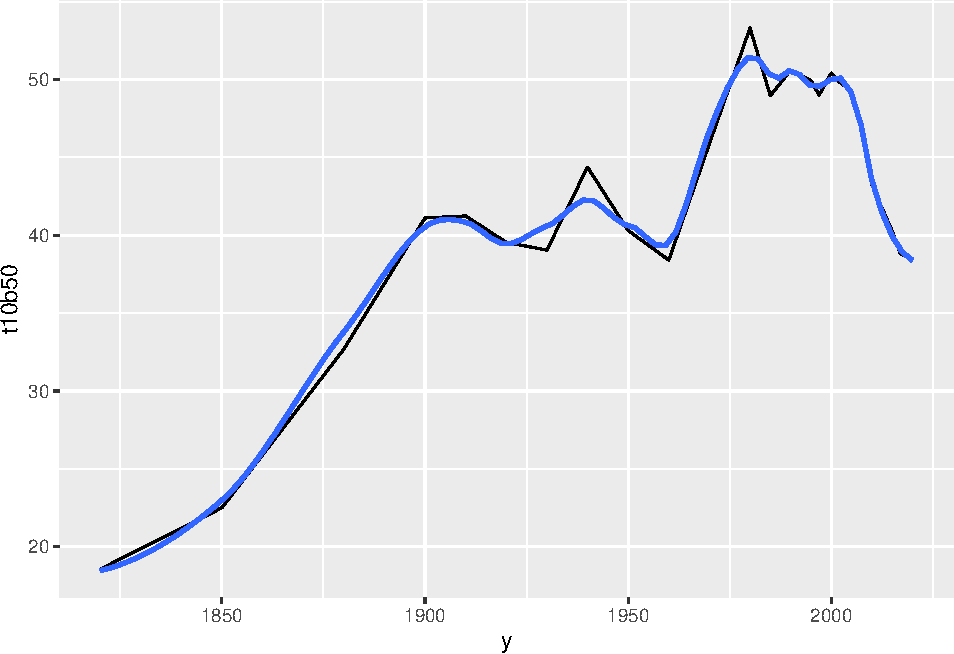
\includegraphics{03-first-example_files/figure-latex/unnamed-chunk-29-1.pdf}

\hypertarget{ux7df4ux7fd2}{%
\section{練習}\label{ux7df4ux7fd2}}

\begin{enumerate}
\def\labelenumi{\arabic{enumi}.}
\tightlist
\item
  それぞれのグラフから、わかったこと、問いなどを列挙してみましょう。
\item
  Fig 1 の Japan の部分を他の国や、グループ(World など)に変えてみてください。何がわかりますか。
\item
  Fig 3 の iso2c で選択する、国を変更してください。何がわかりますか。
\item
  Fig 4 または Fig 5 の iso2c の部分を他の国に変更してください。何がわかりますか。
\item
  Fig 5 または Fig 6 の、区間の幅や、数を 変更してみてください。何がわかりますか。
\item
  Fig 7, Fig 8, Fig 9 の年を変更してみてください。何がわかりますか。
\item
  Fig 12, Fig 13 の年を変更してみてください。何がわかりますか。
\end{enumerate}

\hypertarget{ux30d7ux30edux30b8ux30a7ux30afux30c8}{%
\section{プロジェクト}\label{ux30d7ux30edux30b8ux30a7ux30afux30c8}}

他のデータで、同様のことをしてみましょう。

\begin{enumerate}
\def\labelenumi{\arabic{enumi}.}
\tightlist
\item
  最初に、\texttt{gdp\ =\ "NY.GDP.MKTP.CD"} としましたが、GNI per capita, Atlas method (current US\$): NY.GNP.PCAP.CD に変えてみましょう。
\end{enumerate}

\begin{Shaded}
\begin{Highlighting}[]
\NormalTok{df\_gnppcap }\OtherTok{\textless{}{-}} \FunctionTok{WDI}\NormalTok{(}\AttributeTok{country =} \StringTok{"all"}\NormalTok{, }
              \AttributeTok{indicator =} \FunctionTok{c}\NormalTok{(}\AttributeTok{gnppcap =} \StringTok{"NY.GNP.PCAP.CD"}\NormalTok{), }
              \AttributeTok{extra =} \ConstantTok{TRUE}\NormalTok{)}
\end{Highlighting}
\end{Shaded}

\begin{enumerate}
\def\labelenumi{\arabic{enumi}.}
\setcounter{enumi}{1}
\tightlist
\item
  \href{https://datatopics.worldbank.org/world-development-indicators/}{World Development Indicators} のサイトの下にある、Data Themes(テーマ)から自分が調べたいテーマを選び、そのテーマから、データコードを取得して、同様の分析をしてみてください。データがあまりない場合もありますので、ある程度データが多いものを選択することをお勧めします。
\end{enumerate}

\hypertarget{ux307eux3068ux3081}{%
\section{まとめ}\label{ux307eux3068ux3081}}

今回は、経済指標である、GDP を使いました。データサイエンスについて少しずつ、学んでいきます。

コードの説明は、簡単にしかしていませんから、理解するのは難しいと思いますが、いくつかのことは、ご理解いただけると思います。

\begin{itemize}
\item
  それほど、長くはない、コードで、データを見ていく。R は対話型(interactive)のプログラミング言語と言われています。
\item
  コードに続けて、結果が表示されるので、コードと出力の対応が見やすい。また、コメントや説明も併記することができる。これは、RMarkdown という形式の中で、コードを書いていることによるものです。RMarkdown は、再現性(reproducibility)と、プログラム・コードの内容をコンピュータにわかるようにでなく、人間にもわかるように記述する(Literate Programming)を実現しています。
\item
  視覚化(Visualization)によって、わかることが色々とある。また、視覚化の方法もたくさんあり、いろいろな見方をすることで、データについての理解が深まっていく。
\item
  視覚化を通して、データを理解すること、問いを持ち、他の視覚化などを用いて、さらに、理解を深めることがたいせつ。
\item
  理解したことを元にして、さらに、そのデータ、または、他のデータを使って、新たな発見をしていく。
\end{itemize}

統計的な指標も用いますが、それらによって、新しい知識を生み出すとも表現しますが、そのような営み全体が、データサイエンスの核をなす部分だと思います。

\hypertarget{wdi-site}{%
\chapter{世界開発指標とオープンデータ}\label{wdi-site}}

最初の例として紹介した、\href{https://icu-hsuzuki.github.io/ds4aj/first-example.html\#first-example}{はじめてのデータサイエンス}では、世界銀行(World Bank)の 世界開発指標(WDI)のひとつである、GDP(Gross Domestic Product 国内総生産)のデータを使いました。「データサイエンスをはじめましょう」では、世界開発指標をこれからも、頻繁に活用しますので、世界開発指標が、どのようなものか確認しておきましょう。

また、世界開発指標に代表されるオープンデータによって誰でも世界の課題を知り、向き合うことができるようになっています。そのオープンデータは、どのようなものなのかも、見ていきたいと思います。

\hypertarget{ux4e16ux754cux958bux767aux6307ux6a19wdi}{%
\section{世界開発指標(WDI)}\label{ux4e16ux754cux958bux767aux6307ux6a19wdi}}

世界開発指標は、貧困撲滅と開発援助とに取り組んでいる金融機関である世界銀行が提供している、オープンデータの一つで、世界銀行は、他にも、たくさんのデータを提供しています。

世界開発指標は、英語では、World Development Indicators(WDI)と呼びますので、以下、省略形の WDI を使います。

\hypertarget{ux6982ux8981}{%
\subsection{概要}\label{ux6982ux8981}}

まず、簡単に概要を述べておきましょう。

\href{https://datatopics.worldbank.org/world-development-indicators/}{World Development Indicators (WDI)} は、世界銀行が開発に関する各国間比較可能なデータの集大成である1400の時系列指標(the World Bank's premier compilation of cross-country comparable data on development; 1400 time series indicators)からなっており、それらは、テーマ別にも分類されています。

また、さまざまな形式(CSV, Excel など)で、データを検索し、ダウンロードできるように整理されており、さらに、API (Application Program Interface:アプリケーションのプログラムを使ってデータを利用するための仕様)も整備されており、「データサイエンスをはじめましょう」で利用する コンピュータ言語 R でも、簡単に、検索やデータのダウンロードが可能なパッケージが提供されています。

\hypertarget{ux4e09ux3064ux306eux5165ux308aux53e3}{%
\subsection{三つの入り口}\label{ux4e09ux3064ux306eux5165ux308aux53e3}}

\begin{itemize}
\tightlist
\item
  \href{https://datatopics.worldbank.org/world-development-indicators/}{世界開発指標(WDI)} (World Development Indicators)
\item
  \href{https://data.worldbank.org}{世界銀行オープンデータ} (World Bank Open Data)
\item
  \href{http://wdi.worldbank.org/tables}{世界開発指標(WDI)の統計表} (World Development Indicators Statistical Tables)
\end{itemize}

三つのサイトのリンクを書きました。一つ一つみていきましょう。

まず、英語を読むことが苦手な場合は、ブラウザー(Google Chrome, Edge, Safari などのホームページ閲覧ソフト)の自動翻訳機能を使うのも良いでしょう。しかし、自動翻訳機能を利用していると、リンク先に飛べなかったり、いくつかの機能が使えないこともありますので、正常に機能しないときは、自動翻訳機能を一旦 OFF にして利用してください。

\hypertarget{ux4e16ux754cux958bux767aux6307ux6a19wdi-1}{%
\subsection{\texorpdfstring{\href{https://datatopics.worldbank.org/world-development-indicators/}{世界開発指標(WDI)}}{世界開発指標(WDI)}}\label{ux4e16ux754cux958bux767aux6307ux6a19wdi-1}}

まずは、この\href{https://datatopics.worldbank.org/world-development-indicators/}{サイト}がお薦めです。上の方に以下のように書かれています。

\begin{quote}
The World Development Indicators is a compilation of relevant, high-quality, and internationally comparable statistics about global development and the fight against poverty. The database contains 1,400 time series indicators for 217 economies and more than 40 country groups, with data for many indicators going back more than 50 years.

世界開発指標は、世界的な開発と、貧困との闘いに関連する、高品質で、国際的に比較可能な統計をまとめたものです。データベースには、217の経済と40以上の国グループの1,400の時系列指標が含まれており、多くの指標のデータは50年以上前にさかのぼることができます。
\end{quote}

この文章の下には、テーマ別のアイコンがあり、そこから、それぞれのテーマについてみていくことができるようになっています。さらにその下には、最近のニュースやお薦めの記事などが掲載されています。

\hypertarget{ux30c6ux30fcux30deux3055ux307eux3056ux307eux306aux30c8ux30d4ux30c3ux30afux8ab2ux984c}{%
\subsubsection{\texorpdfstring{\href{https://datatopics.worldbank.org/world-development-indicators/}{テーマ}(さまざまなトピック・課題)}{テーマ(さまざまなトピック・課題)}}\label{ux30c6ux30fcux30deux3055ux307eux3056ux307eux306aux30c8ux30d4ux30c3ux30afux8ab2ux984c}}

\begin{enumerate}
\def\labelenumi{\arabic{enumi}.}
\tightlist
\item
  貧困と不平等(Poverty and Inequality):貧困、繁栄、消費、所得分配
\item
  人々(People):人口動態、教育、労働、健康、ジェンダー
\item
  環境(Environment):農業、気候変動、エネルギー、生物多様性、水、衛生
\item
  経済(Economy):成長、経済構造、所得と貯蓄、貿易、労働生産性
\item
  国家と市場(States and Markets):ビジネス、株式市場、軍事、通信、輸送、テクノロジー
\item
  グローバルリンク(Global Links):債務、貿易、援助への依存、難民、観光、移住
\end{enumerate}

\hypertarget{ux305dux308cux305eux308cux306eux30c6ux30fcux30deux306bux3064ux3044ux3066}{%
\subsubsection{それぞれのテーマについて}\label{ux305dux308cux305eux308cux306eux30c6ux30fcux30deux306bux3064ux3044ux3066}}

一つテーマを選んで中身をみてみましょう。テーマを選んで、中身をみてみると、一番上に、最近のトピックなどが書かれ、次に、そのテーマについての概要や課題が書かれています。データの集め方や、どのように標準化するかなどについての説明もあります。

その下に、注目の指標(Featured Indicators)として、主要な WDI の指標のリストがあり、さらにその下には、データについての説明などが書かれています。

\hypertarget{ux6ce8ux76eeux306eux6307ux6a19featured-indicators}{%
\subsubsection{注目の指標(Featured Indicators)}\label{ux6ce8ux76eeux306eux6307ux6a19featured-indicators}}

この指標も、いくつかのグループに分けられていますが、それぞれの指標には、以下のような情報があります。

\begin{itemize}
\item
  Indicator 指標の名称

  \begin{itemize}
  \tightlist
  \item
    マウスを当てると、より詳しい概要をみることができます。
  \end{itemize}
\item
  Code 指標コード

  \begin{itemize}
  \item
    R の WDI パッケージなど、API を利用して、データを取得するときに必要なコードです。
  \item
    このコードをクリックすると、World(世界)に関する、この指標のデータをグラフが表示されます。世界に対応するデーががない場合もあります。
  \end{itemize}
\item
  Time coverage どの程度の期間のデータがあるかの概要

  \begin{itemize}
  \tightlist
  \item
    1960年から10年刻みでデータがどの程度あるかを確認することができます。
  \end{itemize}
\item
  Region coverage 地域ごとのデータの収集状況の概要

  \begin{itemize}
  \tightlist
  \item
    ラテンアメリカ、南アジア、サハラ砂漠以南のアフリカ、ヨーロッパと中央アジア、中東と北アフリカ、東アジアと太平洋諸国、北アメリカごとに、データがどの程度揃っているかを確認することができます。
  \end{itemize}
\item
  Get data データの取得

  \begin{itemize}
  \tightlist
  \item
    API、XLS、CSV、DataBank とあり、データを、取得するための情報や、Excel、コンマで区切られてテキストデータが取得可能で、また、DataBank では、World Bank のデータの、表や、グラフ、地図、各データの情報などを調べることができます。この DataBank の利用については、別の項で説明します。
  \end{itemize}
\end{itemize}

\hypertarget{ux5099ux8003}{%
\subsubsection{備考}\label{ux5099ux8003}}

はじめてのデータサイエンスで利用した、GDP の指標は、テーマから経済(Economy)を選択すると、Featured Indicator (注目の指標)の一番上にあります。まずは、GDP について、上に書いた、Indicator、Code、Time Coverage、Region Coverage、GetData を確認することをお勧めします。

このサイトにあるのは、基本的な指標だけです。すべての指標についての情報を得るときには、この次とその次の項目を見てください。しかし、全体では、1400も指標があり、何をみたらよいか、かえって混乱してしまうかもしれません。まずは、このような基本的なデータで、使い方を把握してから、興味のあるデータを調べるのが良いと思います。

また、基本的な指標を調べると、その指標のページから関連した指標についても調べることができます。

WDI は、すべての年、すべての国についてのデータがあるわけではありません。前もって、期間や、地域ごとにどの程度データがあるかを見ておくことはとても有効です。

それぞれの指標についての概要や特定の国についての情報は、次の項目から見ることも可能です。このページに掲載されている指標で興味をもったものについて、指標の名称や指標コードをコピー・ペーストなどで、記録しておくことをお勧めします。

\hypertarget{ux4e16ux754cux9280ux884cux30aaux30fcux30d7ux30f3ux30c7ux30fcux30bf}{%
\subsection{\texorpdfstring{\href{https://data.worldbank.org}{世界銀行オープンデータ}}{世界銀行オープンデータ}}\label{ux4e16ux754cux9280ux884cux30aaux30fcux30d7ux30f3ux30c7ux30fcux30bf}}

世界銀行のオープンデータ全体にアクセスできるサイトです。

その下には、いくつかのグラフや、最近のニュースやトピックが書かれており、さらにその下には、More Resources(さらに\ldots)といくつかの項目があります。Open Data Catalog、Data Bank、などと共に、World Development Indicators もあります。このWorld Development Indicators (WDI) を選択すると、最初に紹介したサイトに飛ぶことができます。また、Data Bank を選択すると、WDI の説明に登場した、ダッシュボートに飛ぶことができ、WDI だけでなく、他のデータについても、調べることができます。

上の検索窓の下に、Country(国)と Indicators(指標)と書いてあります。これらから、WDI について調べることができます。

\hypertarget{ux56fdux5225ux30b5ux30a4ux30c8}{%
\subsubsection{\texorpdfstring{\href{https://data.worldbank.org/country}{国別サイト}}{国別サイト}}\label{ux56fdux5225ux30b5ux30a4ux30c8}}

Country(国別)のサイトを選択すると、国のリストが出てきます。

J のところに、Japan(日本)がありますから、選択してみてください。日本のさまざまな指標と小さなグラフが出てきます。

Indicator(指標)、Most Recent Values(直近の値)、Trend(傾向)が表示されます。指標をクリックすると、大きなグラフが出てきます。その指標のサイトですから、そこで、その指標についての他の国の状況などを確認することができます。そこでは、選択した指標と似た指標が選択できたり、もっと詳しいことをしらべるデータバンク(Data Bank)へのリンクもあります。このサイトから、データをダウンロードすることもできるようになっています。

また、\href{https://data.worldbank.org/country}{国別サイト}の右の方には、地域や、経済的状況などによって、グループに分けてある帯もあります。その一番下には、World (世界)もありますから、世界全体について見てみたり、6段階の収入(GNI per Capita:一人当たりの国民総生産)の階級に分けた階級ごとの値を見ることもできるようになっています。

\hypertarget{ux6307ux6a19ux5225ux30b5ux30a4ux30c8}{%
\subsubsection{\texorpdfstring{\href{https://data.worldbank.org/indicator}{指標別サイト}}{指標別サイト}}\label{ux6307ux6a19ux5225ux30b5ux30a4ux30c8}}

Indicators(指標)を選択すると、トピックに分けて、指標が並んでいます。

よく見ると、一番上に、Featured Indicators(特徴的な指標) と、All Indicators(すべての指標) とあり、最初に開いているのは、特徴的な指標の方であることがわかります。すべての指標(All Indicators)の方を開けると、よりたくさんの指標を見ることができます。

トピックは、以下のものに分かれています。

\begin{itemize}
\tightlist
\item
  Agriculture \& Rural Development 農業と農村開発
\item
  Aid Effectiveness 援助の有効性
\item
  Climate Change 気候変動
\item
  Economy \& Growth 経済と成長
\item
  Education 教育
\item
  Energy \& Mining エネルギーと鉱業
\item
  Environment 環境
\item
  External Debt 対外債務
\item
  Financial Sector 金融セクター
\item
  Gender 性別
\item
  Health 健康
\item
  Infrastructure インフラ
\item
  Poverty 貧困
\item
  Private Sector 民間部門
\item
  Public Sector 公共部門
\item
  Science \& Technology 科学技術
\item
  Social Development 社会開発
\item
  Social Protection \& Labor 社会的保護と労働
\item
  Trade 貿易
\item
  Urban Development 都市開発
\end{itemize}

それぞれの指標を選択すると、グラフが表示される画面が出てきます。それは、上で国別のところから選択したものと同じです。

はじめてのデータサイエンスで、GDP を調べるときには、Economy and Growth のトピックにある、\href{https://data.worldbank.org/indicator/NY.GDP.MKTP.CD?view=chart}{GDP (current US\$)} のWDI コード NY.GDP.MKTP.CD を指定して、データを取得しました。この、Indicator Code (WDI コード)は、Details (詳細) を見ると、その指標の概要とともに、書いてあります。 そのデータコードは、そのページの上の URL にも表示されています。

WDI という R のパッケージを使って、データを読み込みました。そのときに必要だったのが、この Indicator Code (WDI コード)でした。あとで、詳しく調べてみたい指標がありましたら、その 指標名(Indicator Name)と、WDIコード(Indicator Code)を、使えるように、メモなどに貼り付けて(Copy-Paste)おくことを、お勧めします。

\hypertarget{ux4e16ux754cux958bux767aux6307ux6a19wdiux306eux7d71ux8a08ux8868}{%
\subsection{\texorpdfstring{\href{http://wdi.worldbank.org/tables}{世界開発指標(WDI)の統計表}}{世界開発指標(WDI)の統計表}}\label{ux4e16ux754cux958bux767aux6307ux6a19wdiux306eux7d71ux8a08ux8868}}

三つ目の入り口の説明をしましょう。英語名は、World Development Indicators Statistical Tables となっています。WDI の一番下の、Useful Resouces (資料)の中にもありますし、それぞれの、テーマの中にもリンクがあります。

世界開発指標(WDI)の統計表 の\href{http://wdi.worldbank.org/tables}{リンク}を開くと、WDI が7つのグループに分けられています。

\begin{enumerate}
\def\labelenumi{\arabic{enumi}.}
\item
  World View 世界の姿
\item
  Poverty and Shared Prosperity 貧困と富の分配
\item
  People 人々
\item
  Environment 環境
\item
  Economy 経済
\item
  States and Market 国と市場
\item
  Global Links 世界の繋がり
\end{enumerate}

WDI のテーマとほぼ一致しています。それぞれのテーマを選択すると、その説明とともに、さらに項目に分かれており、そのデータを見たり、データを PDF または Excel 形式で、ダウンロードして利用できるようになっています。

\hypertarget{ux8ab2ux984c}{%
\subsection{課題}\label{ux8ab2ux984c}}

世界開発指標(WDI)の、データで、調べてみたい データコードをいくつか見つけて、書き出してください。あとで利用しやすいように、データ名と、WDI コードをコピーして、メモ帳などに貼り付けておくと良いでしょう。さらに、そのコードに関する情報やリンクを、一緒に記録としておくと、あとで便利です。

\hypertarget{ux30aaux30fcux30d7ux30f3ux30c7ux30fcux30bfopen-data}{%
\section{オープンデータ(Open Data)}\label{ux30aaux30fcux30d7ux30f3ux30c7ux30fcux30bfopen-data}}

世界開発指標(WDI)のように、公開されているデータを、オープンデータと呼びます。世界銀行などの、国際機関や、国際的に活動する非営利団体、それぞれの国の公的機関が、膨大なデータを公開(オープンに)し、誰でも利用できるようになってきています。

パブリックデータ(Public Data)とも呼ばれますが、正確な定義があるわけではなく、各機関によって、少しずつ考え方が違う面もあります。しかし、そのリーダーとでもいうべき、世界銀行は、オープンデータについて、厳密に定義をしています。

世界銀行のオープンデータ(Open Data)の定義を見てみましょう。

\hypertarget{ux30aaux30fcux30d7ux30f3ux30c7ux30fcux30bfux306eux5b9aux7fa9open-data-defined}{%
\subsection{\texorpdfstring{オープンデータの定義(\href{http://opendatatoolkit.worldbank.org/en/essentials.html}{Open Data Defined})}{オープンデータの定義(Open Data Defined)}}\label{ux30aaux30fcux30d7ux30f3ux30c7ux30fcux30bfux306eux5b9aux7fa9open-data-defined}}

オープンデータという言葉は、厳密な意味を持っています。データまたはコンテンツは、出所が明示されオープンという性質が維持されれば、誰でも自由に利用、再利用、再配布できるものを言います。

\begin{enumerate}
\def\labelenumi{\arabic{enumi}.}
\item
  データは法的にオープンでなければなりません。つまり、パブリックドメインに置かれ、最小限の制限で自由に使用できなければなりません。
\item
  データは技術的にオープンでなければなりません。つまり、誰でも自由に使える一般的なソフトウェアツールを使ってデータにアクセスし、機械で読み取ることが可読な電子フォーマットで提供されていなければならなりません。パスワードやファイアウォールによる制限を受けずに、公共のサーバーで、だれでもアクセスできなければなりません。また、オープンデータを見つけやすくするために、さまざまな組織がオープンデータカタログを作成し管理してく必要があります。
\end{enumerate}

上の定義で使われている、一つ一つの言葉について、詳細は述べませんが、最初に、はじめてのデータサイエンスで、例を示し、この章で、WDI を例にとって説明してきましたので、みなさんも、基本的な部分は、ご理解いただいたと思います。

\hypertarget{ux30aaux30fcux30d7ux30f3ux30c7ux30fcux30bfux306eux610fux7fa9}{%
\subsection{オープンデータの意義}\label{ux30aaux30fcux30d7ux30f3ux30c7ux30fcux30bfux306eux610fux7fa9}}

一旦、足を止めて、みなさんに考えていただきたいと思います。

\begin{enumerate}
\def\labelenumi{\arabic{enumi}.}
\item
  オープンデータは誰に対してオープン(公開)になっているのでしょうか。
\item
  公的(Pablic)データというとき、公的とはどのような意味でしょうか。
\item
  なぜ、膨大な公的データのオープン化が進み、たいせつにされているのでしょうか。
\end{enumerate}

\hypertarget{ux30aaux30fcux30d7ux30f3ux30c7ux30fcux30bfux306eux5229ux6d3bux7528}{%
\subsection{オープンデータの利活用}\label{ux30aaux30fcux30d7ux30f3ux30c7ux30fcux30bfux306eux5229ux6d3bux7528}}

さまざまな国際機関では、データを、Excel 形式や、CSV (Comma Separated Values)形式などで、提供する以外に、ダッシュボード形式で、グラフを生成するなどして、データの可視化をある程度できるようにしています。さらに、コンピュータのアプリケーションでデータを直接取得できるように、API (Application Program Interface) を提供しています。

世界開発指標(WDI)は、この章で説明してきたように、世界の状況やそれぞれの国についての、1400余のさまざまな指標についてのデータを、長期間にわたって(1960年ごろから)提供している基本的なデータベースで、最初に調べてみることをお勧めします。さまざまな課題を理解するためにも、たいせつだと思います。

さらに、WDI は、この膨大な指標についてのデータすべてを統一した形式で提供しているという特徴があります。したがって、複数の指標についての関係を調べることなども、容易にできます。実は、データサイエンスを始めると、違ったデータを一つにまとめて分析することは、技術的にそれなりに困難があります。それが、WDI では、ほとんどないのです。そのために、非常に使いやすいデータベースになっています。

データを、ダウンロードして、読み込むことが必要になりますが、API が整備されていると、分析ソフト(「データサイエンスをはじめましょう」では R を中心的に使いますが)に直接、取り込むことができるので、データの出所も明確で、他の人も同じように取得できれば、データ自体の、Reproducibility (再現可能性)も担保できます。はじめてのデータサイエンスでも、すべてのコード(コンピュータプログラム)が書かれていたと思います。基本的には、これを、たとえば、コピー、ペーストすれば、皆さんのコンピュータでも同じ結果が得られるということです。これについては、まだ、みなさんは、実感が持てないかもしれませんね。これから、少しずつ、説明していきます。

プログラミング言語 Rを使い始める前に、データに慣れることも大切だと思いますから、次には、さまざまな、オープンデータについて、簡単な説明と共に、付随している、ダッシュボードの利用の仕方も説明しながら、みていきたいと思います。

\hypertarget{notebook}{%
\chapter{データサイエンス ノートブック}\label{notebook}}

データサイエンスの記録について書きます。 また、そのために、必要なツールについても、少しだけ説明します。

この「データサイエンスをはじめましょう」では、R で、自分でコードを書き、R Markdown や、Quarto に記録し、データサイエンスを進めていくことを目指しています。しかし、第一部では、まず、データを見ることに慣れるために、それぞれのサイトが提供する、ダッシュボードを使ってデータを見ていくことを、紹介します。

そのときにも、ノートを作成し、記録をとっていくことは、とても大切です。その説明を少しだけ書きます。

\hypertarget{ux518dux73feux6027ux306eux305fux3081ux306bux8a18ux9332ux3059ux3079ux304dux3053ux3068}{%
\section{再現性のために記録すべきこと}\label{ux518dux73feux6027ux306eux305fux3081ux306bux8a18ux9332ux3059ux3079ux304dux3053ux3068}}

根拠を明確にする(evidence based)ことが、データサイエンスにおいて、必須であることは、すでに、書きました。これから、データを見て行きますが、そのときに、基本的な情報を、記録をしておくことをお勧めします。それが、今後のためにも有用ですし、その習慣をつけることが大切だからです。いくつか、記録すべき項目を書いておきます。

\begin{enumerate}
\def\labelenumi{\arabic{enumi}.}
\item
  日付:そのデータを調べた日付を書いておきます。サイトの内容が変更になる場合もあります。
\item
  データ名:もし、そのデータを特定するデータコードがあれば、それも記録しておきましょう。
\item
  データリンク:インターネット上のアドレスです。ブラウザー(Google Chrome、Edge, Safari などのホームページ閲覧ソフト)の上の窓に、URL(Universal Resource Locator)が表示されますから、それを記録しておきましょう。データ自体の URL を取得できる場合もありますが、そのデータが置かれている、ページ(Website)の URL だけが、取得でき、ダウンロードボタンでダウンロードする形式になっている場合もあります。その場合、右クリックや、Ctrl+Click で、データの、URL が取得できる場合もありますが、できない場合もあります。

  \begin{itemize}
  \tightlist
  \item
    データをダウンロードした時は、そのファイル名と、ダウンロードした日付も忘れずにかいておくことをお勧めします。
  \end{itemize}
\item
  メタデータ:また説明しますが、データには、データについてのデータ(これをメタデータと言います)が付いていることが多いです。最初からすべて記録する必要はありません。上の、データリンクがあれば、必要な時に、戻ることができますから。しかし、データの定義や、変数の定義、データの収集方法などによっては、自分が求めているものではなかったり、データ自体がオリジナルデータではない場合もあります。最初から、詳細を記録する必要はありませんが、注意をはらうことを習慣にしておくことは大切です。
\item
  ダッシュボードを設定したパラメター(何を意味するかは少しずつ説明して行きます):ていねいに、記録するのは、大変ですが、再現には、パラメター情報は、必要です。場合によっては、そのリンクが提供され、そのリンクを使って、同じものが再現できる場合もあります。あるいは、埋め込み(embed)するための iframe link というものが提供されている場合もあります。もし、それがあれば、記録しておいてください。実際には、HTML 文書に埋め込んでも、そのままでは表示できない場合もありますが、設定値が含まれていますので、少し慣れれば、再現することも可能です。
\item
  コメント:そのデータからわかったこと、疑問点、さらに知りたいことなど。少しでも書いてあると、あとで、とても便利です。このようなものが、データサイエンスの核でもありますから、ぜひ、記録しておいてください。
\end{enumerate}

\hypertarget{ux6280ux8853ux7684ux306aux3053ux3068}{%
\section{技術的なこと}\label{ux6280ux8853ux7684ux306aux3053ux3068}}

\hypertarget{ux30d6ux30e9ux30a6ux30b6ux30fcux306eux8a00ux8a9eux3068ux69d8ux3005ux306aux7ffbux8a33ux6a5fux80fd}{%
\subsection{ブラウザーの言語と様々な翻訳機能}\label{ux30d6ux30e9ux30a6ux30b6ux30fcux306eux8a00ux8a9eux3068ux69d8ux3005ux306aux7ffbux8a33ux6a5fux80fd}}

\begin{enumerate}
\def\labelenumi{\arabic{enumi}.}
\item
  ブラウザーの言語:実は、コンピュータのシステム言語が関係しますが、ほとんどの場合、システムの言語は変更せずに、ブラウザーの言語を変更できるようになっています。

  \begin{itemize}
  \item
    Windows でも、Mac でも、Google Chrome が使えますから、Google Chrome で説明すると、「Google Account を管理」から、設定できます。
  \item
    Google Public Data Explorer と検索してみてください。すると、日本語の場合には、ほとんど出てきませんが、英語だと膨大なデータがあります。このサイトの場合には、右上に言語とでますから、言語を英語に変更すると、たくさんのデータを見ることができます。検索エンジンの言語によって、表示されるものが、大きく変化しますから、わたしは、Google のアカウントを複数使って、それぞれで、違う言語設定にしています。言語を変更できるようになると、検索の世界がとても広がります。
  \end{itemize}
\item
  ブラウザーの翻訳機能:最近のブラウザーには、翻訳機能が付属しており、簡単に切り替えることができます。しかし、ブラウザーによって、設定方法が異なりますので、調べて、いつでも使えるようにしておいてください。必要に応じて、翻訳機能の ON/OFF ができるととても便利です。
\item
  \href{https://www.deepl.com/ja/translator}{DeepL} などのアプリの翻訳機能:最近は、ブラウザーの翻訳機能の質も向上しているので、不要かもしれませんが、わたしは、DeepL も併用しています。サイト上でも、翻訳ができますし、アプリをダウンロードして、設定を確認すると、翻訳したい箇所を選択すれば、すぐ翻訳してくれるショートカット機能があります。
\item
  ChatGPT など AI の翻訳機能:最近は、LLM(Large Language Model)の発達で、様々な AI による、翻訳の質も非常に向上しています。ここでは、ChatGPT と書きましたが、他にも様々な AI で、翻訳が可能です。長い文章は、字数を指定して要約をしてもらうことも可能ですから、慣れると世界が広がって行きます。
\end{enumerate}

\hypertarget{ux753bux50cf}{%
\subsection{画像}\label{ux753bux50cf}}

\begin{enumerate}
\def\labelenumi{\arabic{enumi}.}
\item
  グラフのダウンロード:グラフ(graph, chart とも言います)は、画像になっていますから、あとで、利用する場合は、リンクを取得して、そのリンクで同じものを開くことができる場合もありますが、ダウンロードして保存しておくほうが安全です。ダウンロード方法が書いてあったり、右クリックまたは、Ctrl+クリックで、ダウンロードできる場合が多いと思います。また、ダウンロードしたあとに、ノートに貼り付けておくことができれば、そのほうがあとで利用するときに便利です。取得したサイトの URL や、取得した日付も記録しておくことをお勧めします。
\item
  画面収録(Screen Capture):ダウンロードできない場合、その方法が見つからない場合は、画面収録も一つの方法です。Windows, Mac によって方法が異なりますから、あらかじめ調べておくと良いでしょう。
\end{enumerate}

\hypertarget{ux30c7ux30fcux30bfux30d5ux30a1ux30a4ux30eb}{%
\subsection{データファイル}\label{ux30c7ux30fcux30bfux30d5ux30a1ux30a4ux30eb}}

データファイルは、CSV(comma separated values カンマで区切られたテキストデータ)などのテキストデータ、Excel ファイル、または、これらを、圧縮したり、いくつかのファイルをまとめて圧縮したりしてある場合があります。以下、少しだけ、注意点や、確認すべき点を書いておきます。

\begin{enumerate}
\def\labelenumi{\arabic{enumi}.}
\item
  圧縮されている場合の解凍方法を確認しておくこと。Windows か Mac でも違いますから、解凍方法を確認しておいてください。
\item
  CSV が一般的ですが、他にも、区切り文字が、スペースだったり、TAB だったり、縦棒だったりと、様々な形式があります。R を使うようになれば、どの形式であっても、読み込めますし、変換することも可能ですが、二種類の問題が一般的です。

  \begin{itemize}
  \item
    上に書いた区切り文字の違い
  \item
    Encoding の問題。こちらは、日本語などを含むファイルではよく起こる問題です。いわゆる文字化けが生じて中身が読めない場合があります。
  \item
    すべての対策を書くことはできませんが、区切り文字の違いは、Excel の機能でも、解決できます。Microsoft Office も高額なソフトですから、持っていないという場合は、機能限定ですが、Online 版は無料で使えますから、試してみてください。Google Spreadsheet でよみこいむことができる場合もあります。
  \end{itemize}
\end{enumerate}

\hypertarget{ux307eux3068ux3081-1}{%
\section{まとめ}\label{ux307eux3068ux3081-1}}

本書で紹介する、R を使い始めれば、統一した方法で解決できる課題もありますが、記録を取るということは、基本的ですから、簡単に書きました。

上のような記録を何に書くかということは書きませんでした。基本的には、記録を取ることが大切で、何に記録することはあまり、問題ではありません。しかし、リンクを貼り付けて、すぐ開くことができたり、画像を貼り付けたりが、できると便利でしょう。

使い慣れたものを使ってください。できれば、どこでも使えるような Cloud 型のサービスがお勧めです。他の方におすすめを聞くのも良いかもしれません。

次からは、実際に、オープンデータのサイトに行って、データを見ることを経験して行きたいと思います。

\hypertarget{part-ux7b2cux4e00ux90e8-ux30aaux30fcux30d7ux30f3ux30c7ux30fcux30bf}{%
\part{第一部 オープンデータ}\label{part-ux7b2cux4e00ux90e8-ux30aaux30fcux30d7ux30f3ux30c7ux30fcux30bf}}

\hypertarget{publicdata-site}{%
\chapter{オープンデータ}\label{publicdata-site}}

\hypertarget{ux6982ux8981-1}{%
\section{概要}\label{ux6982ux8981-1}}

すでに、オープンデータについて、説明をし、その例として、世界銀行の世界開発指標(World Development Indicators (WDI))の説明をし、その指標の一つである、GDP(Gross Domestic Product 国内総生産)を例にとって、はじめてのデータサイエンスというタイトルで、データサイエンスの実際を見ました。

第一部では、世界銀行や、経済協力開発機構(OECD)、国際連合(United Nations)などの、国際機関のオープンデータや、日本のデータとして、政府機関統計(e-Stat)の紹介をします。

さらに、実際に、それぞれのサイトのオープンデータを、ダッシュボード(dashboard)呼ばれる対話型(Interactive)の機能の使い方を紹介しながら、データを見ていきます。

また、実際のデータの取得(ダウンロード)にも触れ、それぞれの期間が提供する API(アプリケーションプログラムインターフェース)の活用についても、簡単に触れていきます。

第二部で、R を使ったデータサイエンスについて学びますが、その例においても、いくつかのオープンデータを用いる機会がありますので、第一部は、その準備としての位置付けです。オープンデータの分析のより詳しい説明は、第三部で行います。

R を使ったデータサイエンスを、早く学びたい方は、この第一部をスキップして、第二部から読んでくださって構いません。しかし、みなさんの中には、R を使うところまでできるかは自信がないけれど、実際のオープンデータを見て、データサイエンスではどのようなことを考えるのかを体験してみたいという方もおられると思い、第一部を書いています。

また、実際に、オープンデータを活用して、ある課題について調べるときには、基本的なオープンデータについての知識は有用です。どこに、そのようなデータがあるかを見つけることがたいせつであるとともに、データサイエンスはなんと言っても、理論ではなく、実証的なものですから、実際のデータに触れながら、学んでいくのがたいせつだと考えているからです。

第一部の学びを通して、こんなふうに、データがたくさん、公開されているのか、と、そんな感触を持っていただければと思います。

\hypertarget{ux3055ux307eux3056ux307eux306aux6a5fux95a2ux306eux30aaux30fcux30d7ux30f3ux30c7ux30fcux30bf}{%
\section{さまざまな機関のオープンデータ}\label{ux3055ux307eux3056ux307eux306aux6a5fux95a2ux306eux30aaux30fcux30d7ux30f3ux30c7ux30fcux30bf}}

すでに少しだけ紹介した世界銀行以外にも、多くの機関がデータを提供しています。いずれも、使いやすくなってきています。少しずつ、いくつかのデータベースに、アクセスして、できれば、API の利用の仕方も、習得して、データを調べることに少しずつ慣れていっていただければと思います。

下のリストは、私が個人的に、何度か使ったことのある、データベースです。「データサイエンスをはじめましょう」でも、少しずつ消化していきます。他にも、たくさんのデータベースがありますので、ぜひ、調べてみてください。

\begin{itemize}
\tightlist
\item
  国際連合 \href{https://data.un.org}{UNdata}
\item
  経済協力開発機構 \href{https://data.oecd.org}{OECD data}、
\item
  世界格差データベース(World Inequality Database)\href{https://wid.world}{WID}、
\item
  欧州連合の統計局 \href{https://ec.europa.eu/eurostat}{Eurostat}、
\item
  データで見る私たちの世界 \href{https://ourworldindata.org}{Our World in Data}
\end{itemize}

\hypertarget{ux65e5ux672cux306eux30c7ux30fcux30bf}{%
\subsection{日本のデータ}\label{ux65e5ux672cux306eux30c7ux30fcux30bf}}

日本では、それぞれの政府機関でデータを膨大なデータを公開していますが、次のサイトで、それらをまとめて公開しています。

\begin{itemize}
\tightlist
\item
  \href{https://www.e-stat.go.jp/}{e-Stat}:政府統計の総合窓口 - 統計で見る日本
\item
  \href{https://dashboard.e-stat.go.jp}{ダッシュボード}:対話型形式でのデータの視覚化
\end{itemize}

\hypertarget{ux6301ux7d9aux7684ux958bux767aux76eeux6a19sdgs-ux30c7ux30fcux30bf}{%
\subsection{持続的開発目標(SDGs) データ}\label{ux6301ux7d9aux7684ux958bux767aux76eeux6a19sdgs-ux30c7ux30fcux30bf}}

持続的開発目標(Sustainable Development Goals (SDGs))は、皆さんもご存知かと思います。2015年に国際連合で定められ、2030年までの達成目標が掲げられています。様々なサイトがありますから、ご存知かと思いますが、SGDs は、17の分野に分かれており、それぞれにさらに細かい分類があり、その一つ一つに、数値目標が掲げられています。数値目標だけに、依存することは、十分ではないかもしれませんが、少なくとも、その数値目標の達成を検証するために、データが公開されています。

自分が興味をもっている課題に絞って、各サイトでどのようなデータが提供されているかをみていくのもよいと思います。

\begin{itemize}
\tightlist
\item
  世界銀行:\url{https://databank.worldbank.org/source/sustainable-development-goals-(sdgs)}
\item
  国連:\url{https://unstats.un.org/sdgs/dataportal/database}
\item
  データで見る私たちの世界:Our World in Data SGD Tracker: \url{https://sdg-tracker.org/}
\item
  SDG Index: \url{https://dashboards.sdgindex.org/map}
\end{itemize}

\hypertarget{ux30aaux30fcux30d7ux30f3ux30c7ux30fcux30bfux306bux3064ux3044ux3066}{%
\section{オープンデータについて}\label{ux30aaux30fcux30d7ux30f3ux30c7ux30fcux30bfux306bux3064ux3044ux3066}}

オープンデータについては、すでに、世界銀行の定義をご紹介しました。パブリックデータをいう言葉も使われます。それらの違いなども含めて、AI に聞いてみましょう。

\textbf{Q. オープンデータ(Open Data)とか、パブリックデータ(Public Data)と言われるものは、どのようなものですか。定義のようなものと、いくつかの例、さらに、重要視されてきている背景を説明してください。}

\textbf{GPT4.} (2023.8.15)

\textbf{オープンデータ(Open Data)}とは、誰でも自由に利用、再配布、再利用することができ、制限がない、または限定的な制限だけが存在するデータを指します。オープンデータは一般的には無償で提供され、機械可読形式(たとえばCSV、JSONなど)で利用可能であり、再利用のためのライセンスが明確にされています。

一方、\textbf{パブリックデータ(Public Data)}は公共の手段で取得されたデータ、または公共の利益のために公開されるべきデータを指します。これは政府や公共機関、研究機関などが収集したデータで、しばしば公共の利益のために公開されます。

オープンデータとパブリックデータの主な違いは、オープンデータが再利用と再配布の観点から「オープン」であることを強調するのに対し、パブリックデータは単に公開されているだけで、再利用や再配布については必ずしも明示されていないことです。

\textbf{例えば}、以下のようなものがあります:

\begin{enumerate}
\def\labelenumi{\arabic{enumi}.}
\item
  気象データ: 天気予報、気温、風向、風速、降水量など
\item
  交通データ: 交通渋滞、駐車場の利用状況、公共交通機関の運行状況など
\item
  統計データ: 人口、雇用、健康、教育などのデータ
\item
  環境データ: 汚染レベル、森林破壊、気候変動などのデータ
\item
  地理データ: 地図、土地利用、地質学的情報など
\end{enumerate}

オープンデータとパブリックデータが重要視されてきた\textbf{背景}には、以下の要素があります:

\begin{enumerate}
\def\labelenumi{\arabic{enumi}.}
\item
  \textbf{透明性と説明責任}: データが公開されることで、政府や企業の行動についての透明性が高まり、説明責任が強化されます。
\item
  \textbf{イノベーションと経済的価値}: データが自由に利用できることで、新たなビジネスモデルや製品、サービスの開発が促進され、経済的価値が創出されます。
\item
  \textbf{市民参加}: データへのアクセスが提供されることで、市民が社会的・政治的な決定プロセスに参加する機会が増えます。
\item
  \textbf{社会的・環境的課題の解決}: 大量のデータを解析することで、社会的・環境的な課題をより良く理解し、解決策を見つけることが可能になります。
\end{enumerate}

以上のように、オープンデータとパブリックデータは、透明性、説明責任、イノベーション、市民参加、社会的・環境的課題の解決などの観点から重要性を増しています。

\hypertarget{ux30aaux30fcux30d7ux30f3ux30c7ux30fcux30bfux306eux672aux6765}{%
\subsection{オープンデータの未来}\label{ux30aaux30fcux30d7ux30f3ux30c7ux30fcux30bfux306eux672aux6765}}

みなさんは、どのように考えますか。まだ、発展途上で、特に、パブリックデータについては、国によって、考え方も一定ではないように見受けられますが、これから、どのような世界を目指していくのか、データサイエンスは、どのような目的のために必要なのか。みなさんは、なんのために勉強しているのか、上の一つ一つの項目をもとに、周囲のみなさん、友人などと、ディスカッションをしながら、考えていただければと思います。

いずれもたいせつな項目だと思いますが、項目3の市民参加は、公開されているデータをわたしたち市民が利用して初めて可能になることです。項目4の、社会的・環境的課題の解決には、私たち市民も責任をもって、取り組むべきだということが基盤にあるのだと思います。みなさんは、どう考えられますか。

\hypertarget{ux30c0ux30c3ux30b7ux30e5ux30dcux30fcux30c9}{%
\section{ダッシュボード}\label{ux30c0ux30c3ux30b7ux30e5ux30dcux30fcux30c9}}

はじめて、オープンデータを利用するときには、対話型のダッシュボードは、助けとなります。ダッシュボードとはどのようなものか、AI に説明してもらいましょう。

\textbf{Q. データを対話的にみたり視覚化したりする、ダッシュボード(dashboard)について説明してください。}

\textbf{ChatGPT} (2023.08.15)

ダッシュボード(dashboard)は、情報やデータを一元化し、対話的に表示・分析・視覚化できるインタラクティブなユーザーインターフェースです。主にビジネスや組織内で使用され、重要な指標や情報をリアルタイムに監視・分析するために利用されます。

ダッシュボードは、さまざまなデータソースからの情報を収集し、それを一つの場所にまとめて表示します。これにより、膨大なデータを迅速に把握し、傾向やパターンを特定することが可能になります。例えば、売上データ、顧客の統計情報、ウェブ解析データ、ソーシャルメディアの指標など、さまざまなデータソースからの情報を一つのダッシュボードに表示することができます。

ダッシュボードは、視覚化ツールを使用してデータをグラフやチャート、表などの形式で表示します。これにより、データを直感的に理解しやすくし、視覚的なパターンや相関関係を把握することができます。例えば、売上の推移を折れ線グラフで表示したり、地域別の売上を地図上に表示したりすることができます。

ダッシュボードは、利用者が必要な情報に素早くアクセスできるように設計されています。ユーザーは、ダッシュボード上の要素をクリックしたり、フィルタを適用したり、グラフをズームしたりすることで、詳細な情報を取得したり特定の視点でデータを分析したりすることができます。

また、ダッシュボードはリアルタイムな情報の監視にも利用されます。データソースが更新されるたびに、ダッシュボード上の情報も自動的に更新されます。これにより、組織内の関係者が最新の情報にアクセスし、迅速な意思決定を行うことができます。

ダッシュボードは、情報の可視化と分析によって、効率的なデータ駆動型の意思決定を支援する役割を果たします。組織内のさまざまなレベルの利用者が、ビジネスのパフォーマンスを把握し、問題や機会を特定し、戦略やアクションプランを立案するために活用します。

\textbf{Q. 例や、ダッシュボードのサイトを教えてください。}

\textbf{ChatGPT} (2023.8.15)

もちろんです!以下にいくつかのダッシュボードの例と、一般的に使用されるいくつかのダッシュボードサイトをご紹介します。

ダッシュボードの例:

\begin{enumerate}
\def\labelenumi{\arabic{enumi}.}
\item
  Google Analytics: ウェブサイトのトラフィックやユーザー行動などの情報をリアルタイムに監視・視覚化するためのダッシュボードです。
\item
  Salesforce: セールスや顧客関連のデータを統合し、ビジネスのパフォーマンスを追跡するためのダッシュボードです。
\item
  Tableau: データの視覚化と分析に特化したダッシュボード作成ツールであり、さまざまな業界で利用されています。
\end{enumerate}

ダッシュボードのサイト:

\begin{enumerate}
\def\labelenumi{\arabic{enumi}.}
\item
  Klipfolio (\url{https://www.klipfolio.com/})
\item
  Geckoboard (\url{https://www.geckoboard.com/})
\item
  DashThis (\url{https://dashthis.com/})
\item
  Databox (\url{https://databox.com/})
\item
  Microsoft Power BI (\url{https://powerbi.microsoft.com/})
\end{enumerate}

これらのサイトでは、ダッシュボード作成ツールやサービスを利用して、カスタムのダッシュボードを作成することができます。それぞれのサイトには、詳細な情報やデモが提供されている場合もありますので、ぜひご覧ください。

上で、ダッシュボードのサイトとあるのは、これらのサイトのツールを使って、ダッシュボードを作ることができるというものです。少し、ダッシュボードの利用に慣れてきたら、挑戦してみてはいかがでしょうか。

\hypertarget{api-ux3092ux5229ux7528ux3057ux305fux30d1ux30c3ux30b1ux30fcux30b8}{%
\section{API を利用したパッケージ}\label{api-ux3092ux5229ux7528ux3057ux305fux30d1ux30c3ux30b1ux30fcux30b8}}

それぞれのオープンデータを検索したり、読み込んだりするための R のパッケージの紹介をします。上に書いたように、第二部で利用するためです。詳しい使い方は、第三部で紹介します。

基本的には、以下の項目について紹介します。

\begin{itemize}
\item
  R の(公式)パッケージサイト:パッケージも含め、R の管理をしている CRAN の公式サイトの情報です。この下の情報も、ほとんどの場合、このリンク先に掲載されています。
\item
  資料(Materials): README(はじめにお読みください)などで、基本情報が書かれています。
\item
  マニュアル(Manual):利用者用説明書です。パッケージで利用可能な関数(命令、データ)などの情報がすべて書かれてあります。それぞれの関数(命令)に関しては、R Studio 内の Help(ヘルプ検索窓)からも利用可能です。
\item
  使い方の例(Vignette):開発者のサイト(GitHub(バージョン管理システムの支援サイト)など)にある場合もありますが、最近は、公式パッケージサイトに、Vignette として使い方の例が掲載されている場合が増えてきています。すべて理解しようとせず、使い方の例からまずはみてみることが有効です
\end{itemize}

\begin{center}\rule{0.5\linewidth}{0.5pt}\end{center}

\hypertarget{worldbank-site}{%
\chapter{世界銀行(World Bank)}\label{worldbank-site}}

\hypertarget{ux6982ux8981-2}{%
\section{概要}\label{ux6982ux8981-2}}

世界銀行は、貧困削減と持続的成長の実現に向けて、途上国政府に対し融資、技術協力、政策助言を提供する国際開発金融機関です。2030年までに極度の貧困をなくし、各国の下位40パーセントの人々の所得を引き上げて繁栄の共有を促進するという2つの目標を掲げています。

世界銀行の\href{https://www.worldbank.org/en/home}{サイト}を見てみると、下の方にはグラフも出ており、さまざまな統計データを提供することに力を入れていることがわかります。

すでに、世界開発指標については、簡単に説明しました。ここでは、世界銀行のサイトの中のデータについて、見ていくとともに、ダッシュボード(dashboard)の活用、データの取得方法や、API (Application Program Interface)を用いて、R でデータを検索したり、取得するパッケージの紹介を簡単にします。

\hypertarget{ux30c7ux30fcux30bfux30d9ux30fcux30b9}{%
\section{データベース}\label{ux30c7ux30fcux30bfux30d9ux30fcux30b9}}

\hypertarget{ux4e09ux3064ux306eux30b5ux30a4ux30c8}{%
\subsection{三つのサイト}\label{ux4e09ux3064ux306eux30b5ux30a4ux30c8}}

\begin{itemize}
\tightlist
\item
  \href{https://data.worldbank.org}{世界銀行オープンデータ}
\item
  \href{https://datacatalog.worldbank.org/home}{データカタログ}
\item
  \href{https://datatopics.worldbank.org/world-development-indicators/}{世界開発指標(WDI)}
\end{itemize}

一つ一つみていきましょう。

英語を読むことが苦手な場合は、ブラウザー(Google Chrome, Edge, Safari などのホームページ閲覧ソフト)の自動翻訳機能を使うのも良いでしょう。しかし、自動翻訳機能を利用していると、リンク先に飛べなかったり、いくつかの機能が使えないこともありますので、正常に機能しないときは、自動翻訳機能を一旦 OFF にして利用してください。

\hypertarget{ux4e16ux754cux9280ux884cux30aaux30fcux30d7ux30f3ux30c7ux30fcux30bf-1}{%
\subsection{\texorpdfstring{\href{https://data.worldbank.org}{世界銀行オープンデータ}}{世界銀行オープンデータ}}\label{ux4e16ux754cux9280ux884cux30aaux30fcux30d7ux30f3ux30c7ux30fcux30bf-1}}

世界銀行のオープンデータ全体にアクセスできるサイトです。上の検索窓の下に、Country(国)と Indicators(指標)と書いてあります。

その下には、いくつかのグラフや、最近のニュースやトピックが書かれており、さらにその下には、More Resources(さらに\ldots)といくつかの項目があります。Open Data Catalog、Data Bank、などと共に、World Development Indicators もあります。このWorld Development Indicators (WDI) を選択すると、上の三つのサイトの三番目に飛びます。また、Data Bank を選択すると、三つのサイトの二番目に飛びます。

最初に書いた、Country(国)と Indicators(指標)から説明しましょう。

\hypertarget{ux56fdux5225ux30b5ux30a4ux30c8-1}{%
\subsubsection{\texorpdfstring{\href{https://data.worldbank.org/country}{国別サイト}}{国別サイト}}\label{ux56fdux5225ux30b5ux30a4ux30c8-1}}

Country(国別)のサイトを選択すると、国のリストが出てきます。

J のところに、Japan(日本)がありますから、選択してみてください。日本のさまざまな指標とグラフが出てきます。

Indicator(指標)、Most Recent Values(直近の値)、Trend(傾向)が表示されます。指標をクリックすると、大きなグラフが出てきます。その指標のサイトですから、そこで、その指標についての他の国の状況などを確認することができます。そこでは、選択した指標と似た指標が選択できたり、もっと詳しいことを調べるデータバンク(Data Bank)へのリンクもあります。このサイトから、データをダウンロードすることもできるようになっています。

また、国別サイトの右の方には、地域など、グループに分けてある帯もあります。その一番下には、World (世界)もありますから、世界全体について見てみたり、収入の階級に分けたサイトの指標を見ることもできるようになっています。

\hypertarget{ux6307ux6a19ux5225ux30b5ux30a4ux30c8-1}{%
\subsubsection{\texorpdfstring{\href{https://data.worldbank.org/indicator}{指標別サイト}}{指標別サイト}}\label{ux6307ux6a19ux5225ux30b5ux30a4ux30c8-1}}

Indicators(指標)を選択すると、トピックに分けて、指標が並んでいます。

よく見ると、一番上に、Featured Indicators(特徴的な指標) と、All Indicators(すべての指標) とあり、最初に開いているのは、特徴的な指標の方であることがわかります。すべての指標の方を開けると、よりたくさんの指標を見ることができます。

トピックは、以下のものに分かれています。

\begin{itemize}
\tightlist
\item
  Agriculture \& Rural Development 農業と農村開発
\item
  Aid Effectiveness 援助の有効性
\item
  Climate Change 気候変動
\item
  Economy \& Growth 経済と成長
\item
  Education 教育
\item
  Energy \& Mining エネルギーと鉱業
\item
  Environment 環境
\item
  External Debt 対外債務
\item
  Financial Sector 金融セクター
\item
  Gender 性別
\item
  Health 健康
\item
  Infrastructure インフラ
\item
  Poverty 貧困
\item
  Private Sector 民間部門
\item
  Public Sector 公共部門
\item
  Science \& Technology 科学技術
\item
  Social Development 社会開発
\item
  Social Protection \& Labor 社会的保護と労働
\item
  Trade 貿易
\item
  Urban Development 都市開発
\end{itemize}

それぞれの指標を選択すると、グラフが表示される画面が出てきます。それは、上で国別のところから選択したものと同じです。

GDP を調べるときには、NY.GDP.MKTP.CD という、コードを指定して、データを取得しました。この、Indicator Code (WDI コード)は、Details (詳細) を見ると、その指標の概要とともに、書いてあります。 そのデータコードは、そのページの上の URL にも表示されています。

はじめてのデータサイエンスでは、WDI という R のパッケージを使って、データを読み込みました。そのときに必要だったのが、この Indicator Code でした。あとで、詳しく調べてみたい指標がありましたら、その、WDIコード(Indicator Code)を、あとで、使えるように、メモなどに貼り付けて(Copy-Paste)おくことを、お勧めします。

\hypertarget{ux30aaux30fcux30d7ux30f3ux30c7ux30fcux30bfux30abux30bfux30edux30b0open-data-catalog}{%
\subsection{\texorpdfstring{\href{https://datacatalog.worldbank.org/home}{オープンデータカタログ(Open Data Catalog)}}{オープンデータカタログ(Open Data Catalog)}}\label{ux30aaux30fcux30d7ux30f3ux30c7ux30fcux30bfux30abux30bfux30edux30b0open-data-catalog}}

\begin{quote}
The Data Catalog is designed to make World Bank's development data easy to find, download, use, and share. It includes data from the World Bank's~\href{https://microdata.worldbank.org/}{microdata},~\href{http://finances.worldbank.org/}{finances}~and~\href{https://energydata.info/}{energy data}~platforms, as well as datasets from the~\href{https://data.worldbank.org/}{open data catalog.}~There are different ways to access and download datasets.

データカタログは、世界銀行で編纂した開発に関するデータを簡単に検索、ダウンロード、使用、共有できるように設計されています。これには、世界銀行の\href{https://microdata.worldbank.org/}{マイクロデータ}、\href{http://finances.worldbank.org/}{財務}、\href{https://energydata.info/}{エネルギーデータ}プラットフォームからのデータ、および\href{https://data.worldbank.org/}{オープンデータカタログ}からのデータセットが含まれています。データセットにアクセスしてダウンロードするには、さまざまな方法があります。
\end{quote}

世界銀行(World Bank)で編纂したり、他の機関から提供を受けたデータがリストされています。

一番上には、Search Box(検索窓)があり、その下には、Featured (特徴的な、またはお薦め)とあり、いくつものトピックが並んでいます。右に、スクロールするとさらにいくつものトピックを見ることができます。その中にも、上で述べた 世界開発指標(WDI)もありますし、Covid-19 (コロナウイルス感染症)関連のデータもあります。

それぞれの、トピックに、関連のデータがリストされています。

\hypertarget{ux4e16ux754cux9280ux884cworld-bank}{%
\subsection{世界銀行(World Bank)}\label{ux4e16ux754cux9280ux884cworld-bank}}

このページの最初にも書きましたが、簡単にまとめておきましょう。

\begin{itemize}
\tightlist
\item
  世界銀行(World Bank): \url{https://www.worldbank.org}
\item
  \href{https://www.worldbank.org/en/who-we-are}{世界銀行について(Who we are)}:

  \begin{itemize}
  \tightlist
  \item
    極度の貧困状態の削減(To end extreme poverty): 2030年までに、極度の貧困状態にある世界人口の割合を3\%に削減する。By reducing the share of the global population that lives in extreme poverty to 3 percent by 2030.
  \item
    繁栄を共に享受(To promote shared prosperity): すべての国の最貧困層の40%の人々の所得を増加させることによって共栄を促進。By increasing the incomes of the poorest 40 percent of people in every country.
  \end{itemize}
\item
  世界銀行オープンデータ(World Bank Open Data): \url{https://data.worldbank.org}

  \begin{itemize}
  \tightlist
  \item
    Data Bank, World Development Indicators, etc.
  \end{itemize}
\end{itemize}

日本について:\url{https://data.worldbank.org/country/japan?view=chart}

\hypertarget{ux4e16ux754cux958bux767aux6307ux6a19world-development-indicator}{%
\subsection{世界開発指標(World Development Indicator)}\label{ux4e16ux754cux958bux767aux6307ux6a19world-development-indicator}}

すでに紹介しましたが、簡単にまとめておきます。

\begin{itemize}
\tightlist
\item
  \href{https://datatopics.worldbank.org/world-development-indicators/}{World Development Indicators (WDI)} : 世界銀行が開発に関する各国間比較可能なデータの集大成である1400の時系列指標(the World Bank's premier compilation of cross-country comparable data on development; 1400 time series indicators)

  \begin{itemize}
  \tightlist
  \item
    テーマ別(Themes): 貧困と格差、人間、環境、経済、国家と市場、グローバルリンク集(Poverty and Inequality, People, Environment, Economy, States and Markets, Global Links)
  \item
    オープンデータとデータバンク(Open Data \& DataBank): Explore data, Query database
  \item
    すべてのデータおよびメタデータを Excel または CSV 形式で、一括してダウンロードすることもできるようになっています。Bulk Download:
  \item
    コンピュータを使って読み込む場合のデータの仕様が書かれています。API(Application Program Interface)Documentation
  \end{itemize}
\end{itemize}

1400ものデータがありますから、すべてのデータやメタデータをダウンロードすれば、すぐ、データを調べることができるわけではありません。基本的なことをおく必要がありますね。上にもリンクのある、データカタログから、世界開発指標(World Development Indicators)を選択すると、次のサイトに\href{https://datacatalog.worldbank.org/search/dataset/0037712/World-Development-Indicators}{リンク}がついています。

このページからは、Databank(ダッシュボード)へのリンクなどの他、Excel ファイルや、CSV ファイルで、メタデータを取得することもできるようになっています。WDI 全部のリストもここで見ることができます。このファイルから探すのが最適とは言えませんが、そのようなファイルを持っておくことは便利です。

\hypertarget{ux30c0ux30c3ux30b7ux30e5ux30dcux30fcux30c9dashboard}{%
\section{ダッシュボード(Dashboard)}\label{ux30c0ux30c3ux30b7ux30e5ux30dcux30fcux30c9dashboard}}

世界銀行のダッシュボードには二種類あります。一つは、それぞれの指標についてのダッシュボード、もう一つは、データバンク(DataBank)です。

\hypertarget{world-bank-ux30a2ux30abux30a6ux30f3ux30c8}{%
\subsection{World Bank アカウント}\label{world-bank-ux30a2ux30abux30a6ux30f3ux30c8}}

ダッシュボードは、リンクにアクセスすれば、アカウントなどを作成せず、すぐに使えます。しかし、ダッシュボードを使って、グラフを作成したり、自分用の、データを作成したりした場合には、その結果を、保存をしたり、リンク(iframe 形式)を、文書に埋め込んだりする必要を感じる場合があります。その場合には、一般用アカウントを作成する必要があります。この\href{https://login.worldbankgroup.org/worldbankgroupb2c.onmicrosoft.com/b2c_1_wbg-solexternal_sisu/oauth2/v2.0/authorize?client_id=7077d845-b099-4fca-9f1b-8fcaade1524c\&scope=openid\%20profile\%20offline_access\&redirect_uri=https\%3A\%2F\%2Fpip.worldbank.org\%2Fsol\%2F\&client-request-id=a3010f0e-81e7-45c4-b519-d8e044d3a89b\&response_mode=fragment\&response_type=code\&x-client-SKU=msal.js.browser\&x-client-VER=2.34.0\&client_info=1\&code_challenge=Ome3V78SVvRRXZvJ3DjMvKDuE5CE-N59RHOY09WJ_LY\&code_challenge_method=S256\&nonce=0a59c36f-97dd-4369-a233-544b6a6393eb\&state=eyJpZCI6Ijc3M2MxM2MzLTg5OTItNDEwMS05MmJkLWYyZThmZDQwNjdlZiIsIm1ldGEiOnsiaW50ZXJhY3Rpb25UeXBlIjoicmVkaXJlY3QifX0\%3D}{サイト}の Sign Up から、アカウントを作成してください。

\hypertarget{ux6307ux6a19ux6bceux306eux30c0ux30c3ux30b7ux30e5ux30dcux30fcux30c9}{%
\subsection{指標毎のダッシュボード}\label{ux6307ux6a19ux6bceux306eux30c0ux30c3ux30b7ux30e5ux30dcux30fcux30c9}}

はじめてのデータサイエンスで使った、GDP (Current US\$)、データコード NY.GDP.MKTP.CD についてみてみましょう。

いくつかの方法があります。

\begin{enumerate}
\def\labelenumi{\arabic{enumi}.}
\tightlist
\item
  \href{https://data.worldbank.org}{世界銀行オープンデータ} から、指標(Indicator)を選択し、その中の Economy \& Growth(経済と成長)の中から、\href{https://data.worldbank.org/indicator/NY.GDP.MKTP.CD?view=chart}{GDP (current US\$)} を選択すると、ダッシュボードが現れ、世界の GPD の推移のグラフが表示されます。
\item
  \href{https://data.worldbank.org}{世界銀行オープンデータ} から、国(Country)を選択し、例えば、J から、Japan を選択し、Economics(経済)の指標の \protect\hyperlink{0}{GDP (current US\$)} を選択すると、ダッシュボードが現れ、日本の GDP の推移のグラフが表示されます。指標によっては、上の、Theme(テーマ)や、Topic(トピック)から選ぶ必要がある場合もあります。
\item
  \href{https://datatopics.worldbank.org/world-development-indicators/}{世界開発指標(WDI)}の Data Theme(テーマ)の中の、ECONOMY(経済) の中から、\href{https://data.worldbank.org/indicator/NY.GDP.MKTP.CD?view=chart}{GDP (current US\$)} を選択すると、ダッシュボードが現れ、世界の GPD の推移のグラフが表示されます。
\item
  もし、WDI コード(この場合は、NY.GDP.MKTP.CD)を知っていれば、このコードを、\href{https://data.worldbank.org}{世界銀行オープンデータ} の検索窓に入れて検索すると、上のダッシュボードのページが表示されます。
\end{enumerate}

最初は、選択した指標について、世界か、日本など選択した国の、折れ線グラフ(Line Graph)が表示されていると思います。そして、下の方に、国のリストがあり、その一番下には、地域のリストが続いています\footnote{アルファベットの昇順になっていますが、そのリストの Country(国)の右にある ⌃型のマークを押すと⌵に変わり、降順になります。}。また、Line (折れ線グラフ)と書いた右には、Bar(棒グラフ)と、Map(地図)とあります。

その右には、Also Show (追加)とあり、Aggregates(総合)、Same Region(同じ地域)、Similar Values(近い値)、Highest Values(最高値)、Lowest Values(最小値)を表示することもできます。表示しないときは、None を選択します。

その右には、Share(共有)と、Details(詳細)があります。詳細には、その指標についての、詳しい説明があります。すべてを理解することはできないかもしれませんが、翻訳機能も使って、確認しておくことをお勧めします。詳細には、データコードも書かれています。記録しておくと、次に同じ指標のデータを探すときに便利です。共有からは、Web Page や、SNS に埋め込む、iframe link を取得することができます。

右の方の帯には、関連する指標がリストされ、さらに、Download(ダウンロード)、Data Bank(データバンク)、WDI Tables (統計表)へのリンクがあります。

\hypertarget{ux4f7fux3044ux65b9}{%
\subsubsection{使い方}\label{ux4f7fux3044ux65b9}}

具体例としては、GDP(Current US\$)の世界(World)のグラフが表示されているとします。上の検索窓に GDP(Current US\$)と入っていると思います。

\begin{itemize}
\item
  国や地域の追加

  \begin{itemize}
  \item
    英語で入力しますから、グラフの下の、国や地域名のところから、追加したい、国や地域名を選んで、書き出しておいてください。一つずつ追加するときは、コピーするのも良いかもしれません。
  \item
    日本をグラフに追加するときは、Japan ですから、検索窓に、Japan と入れて\textbf{少し待ちます}。すると、窓の下に、Japan が表示されますから、それを選択(クリック)します。すると、日本のグラフに変わります。India も加えてください。次に、検索窓に、United と入力すると、United Kingdom, United States, United Arab Emirates が表示されますから、United Kingdom を選択してください。Japan, India, United Kingdom の三つの国のグラフが同時に表示されます。これによって、いくつかの国のその指標における経年変化を比較することができます。
  \item
    いろいろな国や地域を加えてみてください。たとえば、GDP を指標として、United States を加えると、United States の GDP の値が大きいため、他の国のグラフは下の方に重なり合うようになります。Afghanistan を加えると、ある年以前のデータがなかったり、値がとても小さいために、X 軸に張り付くようになってしまったりします。みやすいグラフを表示するには、どのようなものの比較をするかも重要になってくることがわかると思います。
  \item
    追加した国や地域を消すのは、単にその国名の、右に表示される x マークを選択すれば良いですし、Delete キーでも消去できます。
  \item
    実は、Japan など一つの国を加えてからあとは、下の国名などのリストから、追加したい国を選択すると、追加されていきます。検索窓に入れるよりも簡単だと思います。
  \end{itemize}
\item
  Also Show の活用

  \begin{itemize}
  \item
    上に書いたように、Aggregates(総合)、Same Region(同じ地域)、Similar Values(近い値)、Highest Values(最高値)、Lowest Values(最小値)を追加できます。たとえば、Japan(日本)だけを残しておいて、Same Region を選択すると、いくつかの国の値が、薄く表示されます。地域名をみると、これは、East Asia \& Pacific(東アジアと太平洋地域)であることが推測されます。
  \item
    そこで、East Asia \& Pasific を選択すると、その地域の総計の値が追加されます。
  \end{itemize}
\end{itemize}

\hypertarget{ux30c7ux30fcux30bfux30c0ux30a6ux30f3ux30edux30fcux30c9}{%
\subsubsection{データダウンロード}\label{ux30c7ux30fcux30bfux30c0ux30a6ux30f3ux30edux30fcux30c9}}

R のパッケージを用いたデータのダウンロードについてはあとから述べますが、指標毎のダッシュボードの右の帯のダウンロードからも、データをダウンロードすることができます。

CSV(Comma Separated Values)、XML(Extensible Markup Language)、EXCEL(Micosoft Excel Spreadsheet) と三つの形式でデータを取得できます。それぞれ、R などで読み込むことができます。ただし、CSV と、XML は、Zip 形式の圧縮ファイルになっています。EXCEL は、三つのシート(Data, Metadata - Countries, Metadata - Indicators)が一つの、ブックになっています。Metadata(メタデータ)は、データのデータで、データについての情報が収められています。

\hypertarget{ux30c7ux30fcux30bfux30d0ux30f3ux30afdatabank}{%
\subsection{データバンク(DataBank)}\label{ux30c7ux30fcux30bfux30d0ux30f3ux30afdatabank}}

上で説明した指標毎のダッシュボードの右の帯からも、データバンクのダッシュボードが開きますが、\href{https://data.worldbank.org}{世界銀行オープンデータ} の下にある、データバンクを選択すると、リストが表示されます。ここで、ある程度選択してから、ダッシュボードを表示させることもできます。一番上に、World Development Indicators(世界開発指標)がありますから、選択してください。あとから、他のものに変更することも可能です。

表が表示され、左の方に、Variables(変数)、Layout(レイアウト)、Styles(形式)、Save(保存)、Share(共有)、Embed(埋め込み) とあり、右上には、Table(表)、Chart(グラフ)、Map(地図)、Metadata(メタデータ) とあり、その下には、Preview(表示)などとなっていると思います。

膨大なデータを選択し、形式を整えて、ダウンロードしたり、グラフを表示したりすることができます。

\hypertarget{ux4f8b1}{%
\subsubsection{例1}\label{ux4f8b1}}

まずは、一つ目の例として、GDP (Current US\$) の値を大きい方から国順に並べてみましょう。

\begin{enumerate}
\def\labelenumi{\arabic{enumi}.}
\item
  Variable の Database で、World Development Indicators を選択します。
\item
  Countries では、上に、All、Countries、Aggregates とありますから、Countries を選択します。
\item
  一番左のチェックボックス Select All(すべて選択)を選びます。これで国が全部選択されました。現在ですと、Selected 217 と出ています。
\item
  Series は、いくつか選択されている可能性がありますから、X マークを選択して、まずは、全部選択を解除し、次に、GDP (current US\$) にチェックを入れます。Selected 1 となっていることを確認してください。
\item
  Time の一番左のチェックボックスから、Select All にしてください。現在では、Selected 63 と表示されました。
\item
  右の方に、Selections have been modified \ldots{} (選択が変更されました \ldots)と出ますので、Apply Changes(変更を適用)を選びます。
\item
  上の Layout タブを選択し、Time を Column(列)、Country を Row(行)、Series を Page(ページに指定します)
\end{enumerate}

ここまでで、Table に、GDP (current US\$) についての表が表示されていることを確認してください。

これを書いている時点では、2022年が最も新しいデータで、2022 の年のところをクリックすると、最初は、国名のアルファベット順になっていると思いますが、それが、その指標の値の、昇順、降順に変更できます。ここでは、GDP が大きな値の順に並べたいので、降順にします。

10位までの国は、United States, China, Japan, Germany, India, United Kingdom, France, Russian Federation, Canada, Italy となっているかと思います。

\href{https://databank.worldbank.org/data/embed/GDP-top-10-in-2022/id/c7fdca3c}{リンク}

\hypertarget{ux4f8b2}{%
\subsubsection{例2}\label{ux4f8b2}}

2022年の値で、10位までの国を選択して、折れ線グラフや、棒グラフなどを書いてみましょう。

\begin{enumerate}
\def\labelenumi{\arabic{enumi}.}
\tightlist
\item
  Variables の Countries の X で選択を解除し、上の10カ国を選んでください。
\item
  右の方に、Selections have been modified \ldots{} (選択が変更されました \ldots)と出ますので、Apply Changes(変更を適用)を選びます。すると表が10カ国のものに変わります。
\item
  上の、Styles を選択し、Chat Type \& Style で、Line(折れ線グラフ)を選択すると、しばらくして、10カ国の、折れ線グラフを表示させることができます。色も変更することも可能です。
\item
  Chat Type \& Style で Horizontal Bar を選択し、Layout で、
\end{enumerate}

\href{https://databank.worldbank.org/Line-graph-of-GDP-of-top-10-countries/id/ff8c5a74}{リンク}

以下では、変数(Variables)の選び方と、グラフ(Chart)について簡単に説明します。

\hypertarget{ux5909ux6570variables}{%
\subsubsection{変数(Variables)}\label{ux5909ux6570variables}}

Database、Country、Series、Time とあり、それぞれの右に、Available と Selected とあります。

どのデータベースについて、国を選択し、系列を選び、期間を選択するという形式になっています。

Database の左の三角印を選択すると、データベース名が確認できます。現在は、World Development Indicators が選択されています。ここで、他のデータベースに変更することも可能ですが、まずは、そのままにしましょう。

次は、Countries(国)です。All、Countries、Aggregates と一番上にあります。国だけを表示するか、地域やグループを表示するか、すべてを表示するかを選択できます。

簡単のために、まずは、Countries(国)を選択しましょう。

国がいくつか選択されている場合もありますから、X マークをクリックして、すべて選択を消去し、国を選んでみましょう。GDP のところで経験したように、GDP の多い方から、United States、China、Japan、Germany、India、United Kingdom、France を選択してみましょう。

\hypertarget{gdp-per-capita-constant-2015-us}{%
\subsubsection{GDP per capita (constant 2015 US\$)}\label{gdp-per-capita-constant-2015-us}}

実質GDP(2015年を基準にしたもの)を、総人口で割った値。アメリカ合衆国、英国、ドイツ、フランス、日本、中国、日本、ロシア、ウクライナの2021年における比較棒グラフ - \href{https://data.worldbank.org/indicator/NY.GDP.PCAP.KD?locations=JP-GB-RU-FR-CN-US-UA-DE\&start=2021\&end=2021\&view=bar}{リンク}

年次変化を示す折線グラフ -

\hypertarget{central-government-debt-total-of-gdp}{%
\subsubsection{Central government debt, total (\% of GDP)}\label{central-government-debt-total-of-gdp}}

2020年の政府の負債(GDP の百分率)- \href{https://data.worldbank.org/indicator/GC.DOD.TOTL.GD.ZS?locations=JP-GB-RU-FR-CN-US-UA-DE\&start=2020\&end=2020\&view=bar}{リンク}

政府の負債(GDP の百分率)の年次変化を示す折線グラフ

\hypertarget{co2-emissions-metric-tons-per-capita}{%
\subsubsection{CO2 emissions (metric tons per capita)}\label{co2-emissions-metric-tons-per-capita}}

CO2 排出量 (1 人あたりのメートル トン) - \href{https://data.worldbank.org/indicator/EN.ATM.CO2E.PC?locations=JP-GB-RU-FR-CN-US-UA-DE\&start=2019\&end=2019\&view=bar}{リンク}

CO2 排出量 (1 人あたりのメートル トン) の年次変化の折線グラフ

\hypertarget{military-expenditure-of-gdp}{%
\subsubsection{Military expenditure (\% of GDP)}\label{military-expenditure-of-gdp}}

2021年の軍事費 (GDP の \%) - \href{https://data.worldbank.org/indicator/MS.MIL.XPND.GD.ZS?locations=JP-GB-RU-FR-CN-UA\&start=2021\&end=2021\&view=bar}{リンク}

軍事費 (GDP の \%) の年次変化

\hypertarget{military-expenditure-current-usd}{%
\subsubsection{Military expenditure (current USD)}\label{military-expenditure-current-usd}}

2021年の軍事費 (現在の米ドル)

軍事費の年次変化

\hypertarget{proportion-of-seats-held-by-women-in-natinal-parliaments}{%
\subsubsection{Proportion of seats held by women in natinal parliaments (\%)}\label{proportion-of-seats-held-by-women-in-natinal-parliaments}}

2021年、国会で女性が占める議席の割合 (\%) - \href{https://data.worldbank.org/indicator/SG.GEN.PARL.ZS?locations=JP-GB-RU-FR-CN-US-UA-DE\&start=2021\&end=2021\&view=bar}{リンク}

国会で女性が占める議席の割合 (\%) の年次変化

\hypertarget{ux4e16ux754cux306eux3055ux307eux3056ux307eux306aux8ab2ux984cux304bux3089ux898bux308b}{%
\subsection{世界のさまざまな課題から見る}\label{ux4e16ux754cux306eux3055ux307eux3056ux307eux306aux8ab2ux984cux304bux3089ux898bux308b}}

\hypertarget{api}{%
\section{API}\label{api}}

世界銀行(World Bank)の API を利用した R のパッケージを二つ紹介します。

\hypertarget{wdi}{%
\subsection{WDI}\label{wdi}}

Search and download data from over 40 databases hosted by the World Bank, including the World Development Indicators (`WDI'), International Debt Statistics, Doing Business, Human Capital Index, and Sub-national Poverty indicators.

世界開発指標(「WDI」)、国際債務統計、Doing Business、人的資本指数、準国家貧困指標など、世界銀行が主催する40以上のデータベースからデータを検索してダウンロードします。

\begin{itemize}
\item
  R のパッケージサイト:\href{https://cran.r-project.org/package=WDI}{https://CRAN.R-project.org/package=WDI}
\item
  資料(Materials):\url{https://cran.r-project.org/web/packages/WDI/readme/README.html}
\item
  マニュアル(Manual):\url{https://cran.r-project.org/web/packages/WDI/WDI.pdf}
\item
  使い方の例:\url{https://vincentarelbundock.github.io/WDI/}
\end{itemize}

\hypertarget{wbstats}{%
\subsection{wbstats}\label{wbstats}}

Programmatic Access to Data and Statistics from the World Bank API

世界銀行APIからのデータと統計へのプログラムによるアクセス

\begin{itemize}
\item
  R のパッケージサイト:\href{https://cran.r-project.org/package=wbstats}{https://CRAN.R-project.org/package=wbstats}
\item
  資料(Materials): \href{https://cran.r-project.org/web/packages/wbstats/readme/README.html}{README}
\item
  マニュアル(Manual):\url{https://cran.r-project.org/web/packages/wbstats/wbstats.pdf}
\item
  使い方の例(Vignette):\url{https://cran.r-project.org/web/packages/wbstats/vignettes/wbstats.html}
\end{itemize}

\hypertarget{google-public-data-explorer}{%
\section{Google Public Data Explorer}\label{google-public-data-explorer}}

\begin{quote}
Google の パブリックデータ探索(Public Data Explorer)サイトの紹介とともに、世界開発指標をこれを使って見てみたいと思います。
\end{quote}

Google で Public Data を検索すると、おそらく、次のサイトが見つかると思います。

\url{https://www.google.com/publicdata/directory?hl=ja\&dl=ja\#!}

これは、日本語サイトで、2023年9月現在では、データの提供元の数が7となっています。また、

右上に、言語とありますから、それで English (United States) を選択すると下のリンクに飛びます。ここには、45と書かれています。

\url{https://www.google.co.jp/publicdata/directory?hl=en_US\&dl=en_US\#!}

英語版で使うことをお勧めします。例えば、上で見た World Development Indicators(世界開発指標)は、英語版だけでなく、日本語版にもありますが、中身を見てみると、国によってデータがなかったり、少し古いデータまでしかなかったりなどあるようです。どの指標の、どのデータとすべてを挙げることはできませんが、英語版を使った方が安全だと思います。指標について、英語で意味するものがよくわからない時は、ブラウザーの翻訳機能を使って見当をつけるのも良いでしょう。

英語版には、上に例が出ていると思います。自動的にスライドしますが、一番最初は、世界開発指標で、私が確認したときは、Living Longer with Fewer Children(子供の数が少ないと長生き)という表題になっています。このグラフをクリックしてください。

\hypertarget{ux4f8b1-wdi-living-longer-with-fewer-children}{%
\subsection{例1 WDI: Living Longer with Fewer Children}\label{ux4f8b1-wdi-living-longer-with-fewer-children}}

グラフをクリックすると、\href{https://www.google.com/publicdata/explore?ds=d5bncppjof8f9_\&ctype=b\&strail=false\&nselm=s\&met_x=sp_dyn_le00_in\&scale_x=lin\&ind_x=false\&met_y=sp_dyn_tfrt_in\&scale_y=lin\&ind_y=false\&met_s=sp_pop_totl\&scale_s=lin\&ind_s=false\&dimp_c=country:region\&ifdim=country\&hl=en_US\&dl=en_US\&iconSize=0.5\&uniSize=0.035}{このようなページ} が表示されると思います。

左の帯には、Public Data、World Development Indicators と書かれ、いろいろな項目が並んでいます。また、よく見ると、以下のように書かれています。

X軸:Life Expectancy(生まれた時点の平均寿命)

Y軸:Fertility Rate(出生率)

色:Region(地域)

サイズ:Population(人口)

下:矢印と2017の数

と出ているかと思います。何が書いてあるか確認してください。違っていても構いません。

これで大体理解できたと思いますが、これが、WDI のデータを元にして、2017年時点での、平均寿命と、出生率の散布図で、丸の大きさで、人口を表し、色で地域を表しています。

下の矢印を押すと、1960から始まって、どのように変化したかを見ることができます。Gapminder のところで、書いた、バブルチャートと言われるもので、ハンス・ロスリングが Google に管理を依頼したと言われています。

左には、Compare by という項目があります。それを開くと、Region、Lending Type、Income Level とあります。Region に Color と書いてあると思いますが、Income Level の右の プルダウンメニューを推し、一番下にある、Color by This を選択すると、右上の、凡例(Legend)と言われるものが、Income Level に変わると思います。動かしてみるとわかりますが、右下に、High Income がまとまっていると思います。日本は、見つけられますか。

Counrtry List のところの、日本にチェックを入れると、Japan と表示されますから、すぐ見つけられます。マウス(ポインター)を丸に近づけると国をみることもできます。High Income でも、Fertility Rate が 2に近い国もあることがわかります。どんな国がそうなっていますか。

この辺りでやめておきます。

右上には、折れ線グラフと、棒グラフと、地球のマークと、散布図のマークがあります。現在は、散布図が使われています。その右には、ギアマークと、リンクのようなマークがあります。

ギアマークで、X軸や、Y軸を対数にしたり、リンクから、このグラフのリンクを取得することもできます。リンクは二種類ありますが、上が、\href{https://www.google.com/publicdata/explore?ds=d5bncppjof8f9_\&ctype=b\&strail=false\&bcs=d\&nselm=s\&met_x=sp_dyn_le00_in\&scale_x=lin\&ind_x=false\&met_y=sp_dyn_tfrt_in\&scale_y=lin\&ind_y=false\&met_s=sp_pop_totl\&scale_s=lin\&ind_s=false\&dimp_c=country:income_level\&idim=country:JPN\&ifdim=country\&tunit=Y\&pit=1504623600000\&hl=en_US\&dl=en_US\&ind=false\&icfg\&iconSize=0.5}{通常のリンク}、下は、iframe リンクと言われるものです。

\hypertarget{ux4f8b2-gdp-per-cap-vs-co2-per-cap-in-log-log}{%
\subsection{例2 GDP per Cap vs CO2 per Cap in Log-Log}\label{ux4f8b2-gdp-per-cap-vs-co2-per-cap-in-log-log}}

今度は、日本語でも、英語でも良いですが、一人当たりの GDP を X 軸に、一人当たりの、CO2 排出量を Y 軸にとり、対数にして、表示してみましょう。

X軸:\textbf{1 人あたり GDP(実質値: 2010 年基準、米ドル表示) - 対数}

Y軸:\textbf{1 人あたりの CO2 排出量 -~対数}

サイズ:人口

色:地域

\href{https://www.google.com/publicdata/explore?ds=d5bncppjof8f9_\&ctype=b\&strail=false\&bcs=d\&nselm=s\&met_s=sp_pop_totl\&scale_s=lin\&ind_s=false\&dimp_c=country:region\&met_y=en_atm_co2e_pc\&scale_y=log\&ind_y=false\&met_x=ny_gdp_pcap_kd\&scale_x=log\&ind_x=false\&idim=country:JPN\&ifdim=country\&tunit=Y\&pit=1409929200000\&ind=false\&icfg\&iconSize=0.5}{リンク}

\hypertarget{ux307eux3068ux3081-2}{%
\subsection{まとめ}\label{ux307eux3068ux3081-2}}

例から始めましたので、二つの WDI の指標を使い、さらに、人口や、地域など、他の指標も、一つのグラフに含めたものを見てきました。最初にすごいものから始めてしまいましたが、大雑把には、次のようなものになっています。

\begin{itemize}
\item
  折れ線グラフ(line graph):一つの指標の時系列での変化。

  \begin{itemize}
  \tightlist
  \item
    いくつかの国や地域などについての値を用いて、色で区別して表示することも可能です。
  \end{itemize}
\item
  棒グラフ(bar graph):一つの指標をいくつかの項目(国や、地域など)を表示

  \begin{itemize}
  \tightlist
  \item
    特定の年の、特定の指標の値を、いくつかの国や地域について表示
  \end{itemize}
\item
  色付き世界地図(choropleth map):カテゴリーごとに、色を変えて、地図上に表示

  \begin{itemize}
  \tightlist
  \item
    個人の収入の多寡などのグループ(income level)ごとに色を変えて、地図上に表示することなどが可能です。
  \end{itemize}
\item
  散布図(scatter plot):二つの指標の関係性を表示

  \begin{itemize}
  \tightlist
  \item
    さらに、点などの大きさにも他の指標の情報を加えたり、色などで、カテゴリーごとの情報を加えることも可能です。
  \end{itemize}
\end{itemize}

最後に一番最初に挙げた、Living Longer with Fewer Children で何種類の情報が表示されているか見てみましょう。同時に、数値か、カテゴリー(グループ)かも書いておきます。

\begin{enumerate}
\def\labelenumi{\arabic{enumi}.}
\item
  Life Expectancy(生まれた時点の平均寿命):数値 - X 軸
\item
  Fertility Rate(出生率):数値 - Y 軸
\item
  Country(国):カテゴリー:点
\item
  Population (人口):数値:点の大きさ
\item
  Region(地域):カテゴリー:点の色
\item
  Year(年):(離散的:とびとびの)数値:一枚ごとのスライド
\end{enumerate}

ほかにはありますか。普通は二つの指標しか表せないように思いますが、ここでは、6つの情報が入っていますね。

いろいろと調べてみませんか。

なかなか素晴らしいですね。ただ、2014年にプロジェクトがスタートしてから、2017年、2020年と更新されていますが、更新の頻度はあまり高くないように見えます。例としては、十分機能していると思いますが。

\hypertarget{oecd-site}{%
\chapter{OECD(経済協力開発機構)}\label{oecd-site}}

\hypertarget{ux6982ux8981-3}{%
\section{概要}\label{ux6982ux8981-3}}

OECD(経済協力開発機構)はヨーロッパ諸国を中心に日・米を含め38ヶ国の先進国が加盟する国際機関です。OECDは国際マクロ経済動向、貿易、開発援助といった分野に加え、最近では持続可能な開発、ガバナンスといった新たな分野についても加盟国間の分析・検討を行っています。

\url{https://www.meti.go.jp/policy/trade_policy/oecd/index.html}

\hypertarget{ux30c7ux30fcux30bfux30d9ux30fcux30b9-1}{%
\section{データベース}\label{ux30c7ux30fcux30bfux30d9ux30fcux30b9-1}}

\hypertarget{oecd}{%
\section{OECD}\label{oecd}}

OECD Data: \url{https://data.oecd.org/}

Topic と Country に分かれて、調べられ、検索も可能です。

\hypertarget{ux30c6ux30fcux30deux5225}{%
\subsection{テーマ別}\label{ux30c6ux30fcux30deux5225}}

\begin{itemize}
\item
  Agriculture

  \begin{itemize}
  \item
    \href{https://data.oecd.org/agriculture.htm\#profile-Agricultural\%20output}{~Agricultural output}
  \item
    \href{https://data.oecd.org/agriculture.htm\#profile-Agricultural\%20policy}{~Agricultural policy}
  \item
    \href{https://data.oecd.org/agriculture.htm\#profile-Fisheries}{~Fisheries}
  \item
    \href{https://data.oecd.org/agriculture.htm\#profile-Sustainable\%20agriculture}{~Sustainable agriculture}
  \end{itemize}
\item
  Development

  \begin{itemize}
  \item
    \href{https://data.oecd.org/drf/total-official-and-private-flows.htm}{Development resource flows}
  \item
    \href{https://data.oecd.org/oda/net-oda.htm}{Official development assistance (ODA)}
  \end{itemize}
\item
  Economy
\item
  Education
\item
  Energy
\item
  Environment
\item
  Finance
\item
  Government
\item
  Health
\item
  Innovation and Technology
\item
  Jobs
\item
  Society
\end{itemize}

\hypertarget{ux4f8b}{%
\subsection{例}\label{ux4f8b}}

OECD Chart: Inflation (CPI), Total / Food / Total less food, less energy, Annual growth rate (\%), Monthly, Jul 2023

OECD Chart: Quarterly GDP, Total, Percentage change, previous period, Quarterly, Q1 2023

\hypertarget{ux30c0ux30c3ux30b7ux30e5ux30dcux30fcux30c9-1}{%
\section{ダッシュボード}\label{ux30c0ux30c3ux30b7ux30e5ux30dcux30fcux30c9-1}}

OECD.Stat \url{https://stats.oecd.org/Index.aspx}

\hypertarget{api-1}{%
\section{API}\label{api-1}}

\hypertarget{un-site}{%
\chapter{United Nations(国際連合)}\label{un-site}}

\hypertarget{ux6982ux8981-4}{%
\section{概要}\label{ux6982ux8981-4}}

\hypertarget{ux30c7ux30fcux30bfux30d9ux30fcux30b9-2}{%
\section{データベース}\label{ux30c7ux30fcux30bfux30d9ux30fcux30b9-2}}

UNdata: \url{https://data.un.org}

膨大なリストがあります。さまざまな機関からデータが提供されていることもあり、WDI のように、規格が統一されてはいません。

\hypertarget{ux30c0ux30c3ux30b7ux30e5ux30dcux30fcux30c9-2}{%
\section{ダッシュボード}\label{ux30c0ux30c3ux30b7ux30e5ux30dcux30fcux30c9-2}}

いくつかのトピックについては、ダッシュボードがあります。

\hypertarget{api-2}{%
\section{API}\label{api-2}}

一部のデータのための API はあります。

\hypertarget{owid-site}{%
\chapter{Our World in Data}\label{owid-site}}

\hypertarget{ux6982ux8981-5}{%
\section{概要}\label{ux6982ux8981-5}}

サイト:\url{https://ourworldindata.org}

様々なトピックについてデータからのレポートがあり、そのデータも見ることができるようになっています。さらに、使いやすい API も提供されています。

一番上の帯の Browse by Topic からトピック探すことができます。

\begin{itemize}
\item
  Population and Demographic Change 人口動態

  \begin{itemize}
  \item
    \href{https://ourworldindata.org/population-growth}{\textbf{Population Growth}}
  \item
    \href{https://ourworldindata.org/age-structure}{\textbf{Age Structure}}
  \item
    \href{https://ourworldindata.org/gender-ratio}{\textbf{Gender Ratio}}
  \item
    \href{https://ourworldindata.org/life-expectancy}{\textbf{Life Expectancy}}
  \item
    \href{https://ourworldindata.org/child-mortality}{\textbf{Child and Infant Mortality}}
  \item
    \href{https://ourworldindata.org/fertility-rate}{\textbf{Fertility Rate}}
  \item
    \href{https://ourworldindata.org/urbanization}{\textbf{Urbanization}}
  \item
    \href{https://ourworldindata.org/migration}{\textbf{Migration}}
  \end{itemize}
\item
  Health 健康
\item
  Energy and Environment エネルギーと環境
\item
  Food and Agriculture 食料と農業
\item
  Poverty and Economic Development 貧困と開発経済
\item
  Education and Knowledge 教育と知識
\item
  Innovation and Technological Change 技術開発とイノベーション
\item
  Living Conditions, Community and Wellbeing 生活環境、共同体と幸せ
\item
  Human Rights and Democracy 人権と民主主義

  \begin{itemize}
  \item
    \href{https://ourworldindata.org/lgbt-rights}{\textbf{LGBT+ Rights}}
  \item
    \href{https://ourworldindata.org/women-rights}{\textbf{Women's Rights}}
  \item
    \href{https://ourworldindata.org/child-labor}{\textbf{Child Labor}}
  \item
    \href{https://ourworldindata.org/human-rights}{\textbf{Human Rights}}
  \item
    \href{https://ourworldindata.org/democracy}{\textbf{Democracy}}
  \item
    \href{https://ourworldindata.org/corruption}{\textbf{Corruption}}
  \end{itemize}
\item
  Violence and War 暴力と戦争

  \begin{itemize}
  \item
    \href{https://ourworldindata.org/biological-and-chemical-weapons}{\textbf{Biological and Chemical Weapons}}
  \item
    \href{https://ourworldindata.org/war-and-peace}{\textbf{War and Peace}}
  \item
    \href{https://ourworldindata.org/military-personnel-spending}{\textbf{Military Personnel and Spending}}
  \item
    \href{https://ourworldindata.org/terrorism}{\textbf{Terrorism}}
  \item
    \href{https://ourworldindata.org/nuclear-weapons}{\textbf{Nuclear Weapons}}
  \item
    \href{https://ourworldindata.org/violence-against-rights-for-children}{\textbf{Violence against children and children's rights}}
  \item
    \href{https://ourworldindata.org/homicides}{\textbf{Homicides}}
  \end{itemize}
\end{itemize}

これら以外にも、コロナウイルス感染症や、持続的開発目標(SDGs)についてのサイトなどもあります。

\hypertarget{ux30ecux30ddux30fcux30c8}{%
\section{レポート}\label{ux30ecux30ddux30fcux30c8}}

\hypertarget{population-growth}{%
\subsection{\texorpdfstring{\href{https://ourworldindata.org/population-growth}{Population Growth}}{Population Growth}}\label{population-growth}}

人口において、日本は、1950年に何番目で、2021年には何番目だかわかりますか。上のダッシュボードからもわかります。

\hypertarget{war-and-peace}{%
\subsection{\texorpdfstring{\href{https://ourworldindata.org/war-and-peace}{War and Peace}}{War and Peace}}\label{war-and-peace}}

1945年以降のデータが主ですが、世界の紛争などの死者数などを知ることができます。古いデータも少しだけあります。

\url{https://ourworldindata.org/war-and-peace\#the-decline-of-wars-between-great-powers}

\hypertarget{ux30c7ux30fcux30bfux30d9ux30fcux30b9-3}{%
\section{データベース}\label{ux30c7ux30fcux30bfux30d9ux30fcux30b9-3}}

owid: \url{https://ourworldindata.org/}

\hypertarget{ux30c0ux30c3ux30b7ux30e5ux30dcux30fcux30c9-3}{%
\section{ダッシュボード}\label{ux30c0ux30c3ux30b7ux30e5ux30dcux30fcux30c9-3}}

\hypertarget{ux4f7fux3044ux65b9-1}{%
\subsection{使い方}\label{ux4f7fux3044ux65b9-1}}

\begin{enumerate}
\def\labelenumi{\arabic{enumi}.}
\item
  Chart グラフ

  \begin{itemize}
  \tightlist
  \item
    いくつかの国(変更可能な場合もあります)についての年次変化を表す折れ線グラフや棒グラフなど
  \end{itemize}
\item
  Choropleth 色付き地図

  \begin{itemize}
  \item
    右上のプルダウンメニューからは、地域(アフリカ、北アメリカ、南アメリカ、アジア、ヨーロッパ、オセアニア)を選択して拡大することができます。
  \item
    それぞれの国にマウスまたはポインターを重ねると、その国の状況を見ることができます。
  \end{itemize}
\item
  Table 表

  \begin{itemize}
  \tightlist
  \item
    データの一部が表となっています。降順・昇順などの並べ替えも可能です。
  \end{itemize}
\item
  Sources 出典

  \begin{itemize}
  \tightlist
  \item
    変数の簡単な定義とともに、World Bank などもともとのデータの出典へのリンクも含まれています。
  \end{itemize}
\item
  Download ダウンロード

  \begin{itemize}
  \tightlist
  \item
    グラフやデータをダウンロードすることができるようになっています。
  \end{itemize}
\item
  Share 共有

  \begin{itemize}
  \tightlist
  \item
    共有リンクや、ホームページに埋め込む iframe リンクなどが付いています。
  \end{itemize}
\end{enumerate}

\hypertarget{covid-19-data-explorer}{%
\subsection{Covid-19 Data Explorer}\label{covid-19-data-explorer}}

\href{https://ourworldindata.org/explorers/coronavirus-data-explorer?zoomToSelection=true\&time=2020-03-01..latest\&facet=none\&country=USA~GBR~CAN~DEU~ITA~IND\&pickerSort=asc\&pickerMetric=location\&Metric=Confirmed+cases\&Interval=7-day+rolling+average\&Relative+to+Population=true\&Color+by+test+positivity=false}{リンク}

日本を加えてあります。

\hypertarget{causes-of-death}{%
\subsection{\texorpdfstring{\textbf{Causes of Death}}{Causes of Death}}\label{causes-of-death}}

死亡原因についての分析のページです。

リンク\url{https://ourworldindata.org/causes-of-death}

\hypertarget{causes-of-death-world-2019}{%
\subsection{\texorpdfstring{\href{https://ourworldindata.org/grapher/annual-number-of-deaths-by-cause}{Causes of death, World, 2019}}{Causes of death, World, 2019}}\label{causes-of-death-world-2019}}

\hypertarget{share-of-deaths-from-major-causes-of-japan-2020}{%
\subsection{\texorpdfstring{\href{https://ourworldindata.org/grapher/share-of-deaths-from-major-causes?country=~JPN}{Share of Deaths from major causes of Japan, 2020}}{Share of Deaths from major causes of Japan, 2020}}\label{share-of-deaths-from-major-causes-of-japan-2020}}

\hypertarget{api-3}{%
\section{API}\label{api-3}}

\begin{itemize}
\item
  パッケージの公式サイト:~\href{https://cran.r-project.org/package=owidR}{https://CRAN.R-project.org/package=owidR}

  \begin{itemize}
  \item
    はじめにお読みください(ReadMe):~\url{https://cran.r-project.org/web/packages/owidR/readme/README.html}
  \item
    マニュアル(Manual):~\url{https://cran.r-project.org/web/packages/owidR/owidR.pdf}
  \item
    使い方の例(Vignette):~\href{https://cran.r-project.org/web/packages/owidR/vignettes/example-analysis.html}{Create and Analyse a Dataset}
  \end{itemize}
\item
  \href{https://rdrr.io/cran/owidR/}{owidR: Import Data from Our World in Data}
\end{itemize}

\hypertarget{estat-site}{%
\chapter{e-Stat 日本の政府統計}\label{estat-site}}

\hypertarget{ux6982ux8981-6}{%
\section{概要}\label{ux6982ux8981-6}}

基本的なデータベースは、「\href{https://www.e-stat.go.jp/stat-search/database?page=1\&layout=normal\&toukei=00200502}{社会・人口統計体系}」から見ることができます。一覧表示も可能ですが、まずは、リンクから階層形式で見ると、都道府県別データと、市町村別データに分かれています。また、それぞれが、基礎データと社会統計指標に分かれ、さらに、それぞれが、

\hypertarget{ux30c7ux30fcux30bfux30d9ux30fcux30b9-4}{%
\section{データベース}\label{ux30c7ux30fcux30bfux30d9ux30fcux30b9-4}}

\begin{itemize}
\tightlist
\item
  \href{https://www.e-stat.go.jp/}{e-Stat}:政府統計の総合窓口 - 統計で見る日本
\item
  \href{https://dashboard.e-stat.go.jp}{ダッシュボード}:対話型形式でのデータの視覚化
\end{itemize}

たくさんの統計が掲載されています。ダッシュボードは、そのうちのいくつかを見やすいように、グラフによって視覚化されています。

まず、\href{https://www.e-stat.go.jp/}{e-Stat} 政府統計の総合窓口に行くと、右上の若葉マークに使い方が書かれていますから、それを読むのがお勧めです。ここには、詳細は書きません。

まず「\href{https://www.e-stat.go.jp/stat-search?page=1}{すべて}」(政府統計一覧)では、すべての統計情報を見ることができ、検索もできます。左の帯に、データベースと、ファイルとありますが。基本的に、API を使って、データを読み込むことができるようになっているのが、データベースです。

その下には、統計分類(大分類)として、トピックごとに分類されたものを調べるものがあります。これは、トップページの「分野」と大体対応しています。その下には、組織で調べる、統計の種類で絞り込み、政府統計名で絞り込み、提供周期で絞り込み、調査年で絞り込み、調査月で絞り込み、50音で絞り込み、統計表フォーマットで絞り込み、集計地域区分で絞り込みと続きます。

まずは、統計の種類から、基幹統計を見てみましょう。\href{https://www.e-stat.go.jp/stat-search?page=1\&toukei_kind=6\&metadata=1\&data=1}{ここ}からも見ることができます。全部で61のデータベース、64のファイルと書かれて、国勢調査や、人口推計、労働力調査、家計調査、学校基本調査などが並んでいます。

\hypertarget{ux5bb6ux8a08ux8abfux67fb}{%
\subsection{家計調査}\label{ux5bb6ux8a08ux8abfux67fb}}

\href{https://www.e-stat.go.jp/stat-search/database?page=1\&toukei=00200561\&tstat=000000330001\&toukei_kind=6\&metadata=1\&data=1}{家計調査}をみてみましょう。家計調査についての説明がありますが、その下の、二人以上の世帯、年次を見てみます。費目分類010 品目分類(2020年改定)(総数:金額)のDB(データベース)をみてみましょう。

表が現れます。

左の方にある、表示項目選択を開きます。

時間軸:すべて解除して、最新の2022のものだけ選択します。

左の方にある、レイアウト設定を開きます。

ページ上部:表章項目、世帯区分、時間軸(年次)

列:費目分類

行:地域分類

確定させてもとに戻ると、それぞれの項目のそれぞれの地域の平均消費額がわかります。一番上には全国平均が載っています。

たとえば、二人以上の世帯の、この調査における平均世帯人数は、2.91人、消費支出3,490,383円、牛乳の支出15,001円などと出ています。

\hypertarget{ux88dcux8db3}{%
\subsubsection{補足}\label{ux88dcux8db3}}

統計表としてではありませんが、家計調査からのランキングのようなものも、公開されています。ご興味のあるかたはみてください。

\href{https://www.stat.go.jp/data/kakei/5.html}{家計調査(二人以上の世帯) 品目別都道府県庁所在市及び政令指定都市(※)ランキング(2020年(令和2年)~2022年(令和4年)平均)}

ただし、このランキングの下になっているデータを探そうとすると、なかなか大変です。

\hypertarget{ux30c0ux30c3ux30b7ux30e5ux30dcux30fcux30c9-4}{%
\section{\texorpdfstring{\href{https://dashboard.e-stat.go.jp}{ダッシュボード}}{ダッシュボード}}\label{ux30c0ux30c3ux30b7ux30e5ux30dcux30fcux30c9-4}}

何種類かのグラフを見ることができると同時に、右の方に、時系列表とあり、これから、データをダウンロードできるようにもなっています。

\href{https://dashboard.e-stat.go.jp/pyramidGraph?screenCode=00570\&regionCode=00000\&pyramidAreaType=2}{人口ピラミッド}

人口ピラミッドを見てみましょう。1920年からの人口ピラミッドを見ることができます。また、日本の全体だけではなく、都道府県、市町村、世界の国々についても見ることができます。ピラミッドの形が変わっていく様子、戦争などで、急激に変化する様子なども、見ることができます。

また、それぞれの個々のグラフのデータをダウンロードすることができます。全体のデータを一括ダウンロードできると良いと思うのですが。

\hypertarget{api-4}{%
\section{API}\label{api-4}}

\hypertarget{estatapi-ux5229ux7528ux6982ux8981}{%
\section{\texorpdfstring{\texttt{estatapi} 利用概要}{estatapi 利用概要}}\label{estatapi-ux5229ux7528ux6982ux8981}}

CRAN \texttt{estatspi} URL: \url{https://CRAN.R-project.org/package=estatapi}

\hypertarget{ux30a2ux30d7ux30eaux30b1ux30fcux30b7ux30e7ux30f3idux306eux8a2dux5b9a}{%
\subsection{アプリケーションIDの設定}\label{ux30a2ux30d7ux30eaux30b1ux30fcux30b7ux30e7ux30f3idux306eux8a2dux5b9a}}

\begin{verbatim}
appId <- " " # 私のものは、英数40文字
\end{verbatim}

\hypertarget{sdgs-site}{%
\chapter{SDGs}\label{sdgs-site}}

持続的開発目標(Sustainable Development Goals)関連の情報がまとまっているサイトの紹介とともに、そのダッシュボードの使い方などデータ関係を中心に書いていきます。

\hypertarget{sdgs-ux3068ux306f}{%
\section{SDGs とは}\label{sdgs-ux3068ux306f}}

\begin{quote}
持続可能な開発目標(SDGs:Sustainable Development Goals)とは,2001年に策定されたミレニアム開発目標(MDGs)の後継として,2015年9月の国連サミットで加盟国の全会一致で採択された「持続可能な開発のための2030アジェンダ」に記載された,2030年までに持続可能でよりよい世界を目指す国際目標です。17のゴール・169のターゲットから構成され,地球上の「誰一人取り残さない(leave no one behind)」ことを誓っています。SDGsは発展途上国のみならず,先進国自身が取り組むユニバーサル(普遍的)なものであり,日本としても積極的に取り組んでいます。(\href{https://www.mofa.go.jp/mofaj/gaiko/oda/sdgs/about/index.html}{外務省ホームページ})
\end{quote}

\hypertarget{ux56fdux969bux9023ux5408}{%
\section{国際連合}\label{ux56fdux969bux9023ux5408}}

17 Goals to Transform Our World: \url{https://www.un.org/sustainabledevelopment/}

SDGs HOME: \url{https://unstats.un.org/sdgs}

国連:\url{https://unstats.un.org/sdgs/dataportal/database}

\hypertarget{ux4e16ux754cux9280ux884c}{%
\section{世界銀行}\label{ux4e16ux754cux9280ux884c}}

世界銀行のダッシュボードとして紹介したデータバンク(DataBank)には、データベースとして、Sustainable Development Goals (SDGs) があります。下のリンクでは、そのデータベースがすでに選択されてあります。

SDGs DataBank:\url{https://databank.worldbank.org/source/sustainable-development-goals-(sdgs)}

全部で408の項目(Series)に分かれて、データを見ることができます。

Data Topics of SDGs: \url{https://datatopics.worldbank.org/sdgatlas/}

17の各項目についての状況がまとめられています。

\hypertarget{owid}{%
\section{OWID}\label{owid}}

データで見る私たちの世界:Our World in Data SGD Tracker: \url{https://sdg-tracker.org/}

17のそれぞれの項目について

\begin{itemize}
\item
  概要
\item
  数値目標と指標
\item
  簡単な解説など
\item
  Chart 視覚化のためのダッシュボード
\end{itemize}

がついています。ダッシュボードについて少し書いておきます。

\begin{enumerate}
\def\labelenumi{\arabic{enumi}.}
\item
  Chart グラフ

  \begin{itemize}
  \item
    いくつかの国についての年次変化を表す折れ線グラフなどがあります。
  \item
    Add Country or Region から国や地域を選択することができるようになっています。
  \end{itemize}
\item
  Choropleth 色付き地図

  \begin{itemize}
  \item
    右上のプルダウンメニューからは、地域(アフリカ、北アメリカ、南アメリカ、アジア、ヨーロッパ、オセアニア)を選択して拡大することができます。
  \item
    それぞれの国にマウスまたはポインターを重ねると、その国の状況を見ることができます。
  \end{itemize}
\item
  Table 表

  \begin{itemize}
  \tightlist
  \item
    データの一部が表となっています。降順・昇順などの並べ替えも可能です。
  \end{itemize}
\item
  Sources 出典

  \begin{itemize}
  \tightlist
  \item
    変数の簡単な定義とともに、World Bank などもともとのデータの出典へのリンクも含まれています。
  \end{itemize}
\item
  Download ダウンロード

  \begin{itemize}
  \tightlist
  \item
    グラフやデータをダウンロードすることができるようになっています。
  \end{itemize}
\item
  Share 共有

  \begin{itemize}
  \tightlist
  \item
    共有リンクや、ホームページに埋め込む iframe リンクなどが付いています。
  \end{itemize}
\end{enumerate}

\hypertarget{ux4f8bsdg1-end-poverty-in-all-its-forms-everywhere}{%
\subsection{\texorpdfstring{例:SDG1: \textbf{End poverty in all its forms everywhere}}{例:SDG1: End poverty in all its forms everywhere}}\label{ux4f8bsdg1-end-poverty-in-all-its-forms-everywhere}}

\href{https://ourworldindata.org/grapher/share-of-population-in-extreme-poverty}{リンク}

\hypertarget{ux4f8bsdg5-achieve-gender-equality-and-empower-all-women-and-girls}{%
\subsection{\texorpdfstring{例:SDG5: \textbf{Achieve gender equality and empower all women and girls}}{例:SDG5: Achieve gender equality and empower all women and girls}}\label{ux4f8bsdg5-achieve-gender-equality-and-empower-all-women-and-girls}}

\href{https://ourworldindata.org/grapher/overarching-legal-frameworks-regarding-gender-equality}{リンク}

\hypertarget{sdg-index}{%
\section{SDG Index}\label{sdg-index}}

SDG Report: \url{https://dashboards.sdgindex.org}

SDG Index: \url{https://dashboards.sdgindex.org/map}

Sustainable Development Report(SDGs 報告)を毎年出しています。17の項目それぞれについての達成度を国別にも確認できるようになっており、改善されている、変化なし、悪化しているなどの状況も掲載されています。

報告全体を読むこともできますが、リンク上の地図で日本を選択すると、日本の状況を見ることができます。SDG1 から SDG17 までの項目について詳しくみていくことも可能です。

指標をどのように決めているかも気になりますが、それを理解するコースも公開しています。

SDGAcademyX: \url{https://www.edx.org/school/sdgacademyx}

\begin{itemize}
\tightlist
\item
  \href{https://www.edx.org/learn/sustainable-development/sdg-academy-measuring-sustainable-development?webview=false\&campaign=Measuring+Sustainable+Development\&source=edx\&product_category=course\&placement_url=https\%3A\%2F\%2Fwww.edx.org\%2Fschool\%2Fsdgacademyx}{Measuring Sustainable Development}
\end{itemize}

\hypertarget{ux5916ux52d9ux7701}{%
\section{外務省}\label{ux5916ux52d9ux7701}}

リンク:\url{https://www.mofa.go.jp/mofaj/gaiko/oda/sdgs/statistics/index.html}

17項目についての説明があり、少し資料もついています。

\hypertarget{other-site}{%
\chapter{その他のサイト}\label{other-site}}

\hypertarget{wir}{%
\section{WIR}\label{wir}}

\hypertarget{ux6982ux8981-7}{%
\subsection{概要}\label{ux6982ux8981-7}}

\hypertarget{ux30c7ux30fcux30bfux30d9ux30fcux30b9-5}{%
\subsection{データベース}\label{ux30c7ux30fcux30bfux30d9ux30fcux30b9-5}}

\hypertarget{ux30c0ux30c3ux30b7ux30e5ux30dcux30fcux30c9-5}{%
\subsection{ダッシュボード}\label{ux30c0ux30c3ux30b7ux30e5ux30dcux30fcux30c9-5}}

\hypertarget{api-5}{%
\subsection{API}\label{api-5}}

\hypertarget{eurostat}{%
\section{EuroStat}\label{eurostat}}

\hypertarget{ux6982ux8981-8}{%
\subsection{概要}\label{ux6982ux8981-8}}

\hypertarget{ux30c7ux30fcux30bfux30d9ux30fcux30b9-6}{%
\subsection{データベース}\label{ux30c7ux30fcux30bfux30d9ux30fcux30b9-6}}

eurostat: \url{https://ec.europa.eu/eurostat}

\hypertarget{ux30c0ux30c3ux30b7ux30e5ux30dcux30fcux30c9-6}{%
\subsection{ダッシュボード}\label{ux30c0ux30c3ux30b7ux30e5ux30dcux30fcux30c9-6}}

\hypertarget{api-6}{%
\subsection{API}\label{api-6}}

\hypertarget{part-ux7b2cux4e8cux90e8-r-ux306eux57faux790e}{%
\part{第二部 R の基礎}\label{part-ux7b2cux4e8cux90e8-r-ux306eux57faux790e}}

\hypertarget{ronrstudio}{%
\chapter{R Studio で R}\label{ronrstudio}}

いよいよ、プログラミング言語 R を使って、データサイエンスを始めます。RStudioで R をすでに、使い始めておられる方も、ざっと読んでおかれることをお勧めします。R Markdown についてと、Posit Cloud というクラウドサービスの利用方法についても、述べてあります。

\hypertarget{ux306fux3058ux3081ux306b}{%
\section{はじめに}\label{ux306fux3058ux3081ux306b}}

この章では、R と R Studio をインストールし、正常に動作しているかを、確認することを目標とします。実際の、使い方は、次の章以下で、述べます。

また、Posit Cloud など、R Studio 以外で、R を使う方法も、最後に述べます。特に、Posit Cloud は、一定の制限はあるものの、基本的には、R Studio で R を使うのと、同様のことが可能な、Cloud 環境ですので、R と R Studio のインストールに成功した場合も、利用方法を確認してください。

確認の段階で、エラーが出てしまった場合の解決方法も、下に書きますが、まずは、Posit Cloud など、他の方法でR を使えるようにして、時間のあるときに、解決を試みてください。

注:\emph{この部分を書いている、2023年では、ほとんど、インストールについては、ほとんど問題がないようですが、Windows ユーザの、OneDrive 問題は、まだ、一部残っているようですので、確認していただくことをお勧めします。}

\hypertarget{r-ux3068-r-studio}{%
\section{R と R Studio}\label{r-ux3068-r-studio}}

\begin{quote}
R is a free software environment for statistical computing and graphics. It compiles and runs on a wide variety of UNIX platforms, Windows and MacOS. \url{https://www.r-project.org}
\end{quote}

\begin{quote}
R は、無償で提供されている、統計解析ともに、データサイエンスにおいてたいせつな可視化のためのグラフを描写する環境でもあります。Windows、MacOS や、Linux で利用することが可能です。
\end{quote}

\begin{quote}
RStudio is an integrated development environment (IDE) for R and Python. It includes a console, syntax-highlighting editor that supports direct code execution, and tools for plotting, history, debugging, and workspace management. RStudio is available in open source and commercial editions and runs on the desktop (Windows, Mac, and Linux). \url{https://posit.co/products/open-source/rstudio/}
\end{quote}

\begin{quote}
RStudio は、R と Python のための、総合開発環境(IDE)です。RStudio には、プログラムを実行したり、制御やジョブ管理のための、コンソール(console)、コードを書いたり、実行したりする、文書の編集をする、エディター(Editor)とともに、グラフを表示したり、履歴や、プログラムを修正するなどのための、さまざまなツールが付属しています。RStudio はオープンソースで提供され、Windows、Mac および、Linux で利用可能で、有償版のサービスと無償版を提供しています。
\end{quote}

R は、統計解析のためのシステムで、R Studio は、R(および Python)を利用するための、総合開発環境です。そこで、「R Studio で R を利用する」という表現をします。

\hypertarget{r-ux3068-r-studio-ux306eux30a4ux30f3ux30b9ux30c8ux30fcux30eb}{%
\section{R と R Studio のインストール}\label{r-ux3068-r-studio-ux306eux30a4ux30f3ux30b9ux30c8ux30fcux30eb}}

R と R Studio をインストールします。

両方とも、インストールすることが必要です。

今後のために、動作確認を、RNotebook を使って行います。

\textbf{注意}

以下は、自分のコンピュータ、すなわち、管理者権限があるコンピュータにインストールすることを前提に書きます。

家族で、コンピュータを共有していて、管理者権限がない場合は、管理者権限のあるかたに、R と RStudio をインストールしてもらってください。そうすれば、そのコンピュータの他のアカウントでも利用することができます。

ある制約がかかるとメッセージが出ますが、管理者権限なしで、インストールすることも可能です。特別の事情があり、管理者権限なしで、インストールする場合は、\href{https://icu-hsuzuki.github.io/myds/techmemo.html\#\%E9\%9D\%9E\%E7\%AE\%A1\%E7\%90\%86\%E8\%80\%85\%E3\%81\%A8\%E3\%81\%97\%E3\%81\%A6-r-\%E3\%81\%A8-rstudio-\%E3\%82\%92\%E3\%82\%A4\%E3\%83\%B3\%E3\%82\%B9\%E3\%83\%88\%E3\%83\%BC\%E3\%83\%AB}{こちら}を参照してください。

\hypertarget{r-ux306eux30a4ux30f3ux30b9ux30c8ux30fcux30eb}{%
\subsection{R のインストール}\label{r-ux306eux30a4ux30f3ux30b9ux30c8ux30fcux30eb}}

\url{https://cloud.r-project.org}

上のリンクから、Windows、macOS または、Linux を選択して、インストールしてください。

Windows の場合は、base - install R for the first time を選択してください。

macOS の場合は、M1, M2 など、最近の Apple Silicon の CPU で動くコンピュータか、以前の、Intel の CPU で動くものか、選択してください。Mac の左上の、りんごマークの、このコンピュータについてから、確認できます。

不明の場合は、「R のインストール」と検索してみてください。

\hypertarget{r-studio-ux306e-ux30a4ux30f3ux30b9ux30c8ux30fcux30eb}{%
\subsection{R Studio の インストール}\label{r-studio-ux306e-ux30a4ux30f3ux30b9ux30c8ux30fcux30eb}}

\url{http://www.rstudio.com/download}

上のリンクから、Windows 10/11 または、macOS 11+ を 選択してください。これら以外の、古いシステムのコンピュータの場合は、 下のサイトから、探してください。

\url{https://docs.posit.co/previous-versions/}

不明の場合は、「RStudio のインストール」と検索してみてください。

\hypertarget{ux52d5ux4f5cux78baux8a8d}{%
\subsection{動作確認}\label{ux52d5ux4f5cux78baux8a8d}}

動作確認のための、一連の流れを書き、その下に、問題が起こった場合の対処を書きます。

R Studio はこれまでも使っていたが、R Notebook は使ったことがないという方も、同様の確認をしてください。

\begin{enumerate}
\def\labelenumi{\arabic{enumi}.}
\tightlist
\item
  RStudio を立ち上げます。
\item
  上のメニューの File から、New Project を選択します。
\item
  Project の名前を(test とか、firstproject など)つけて、Create ボタンを押します。
\item
  上のメニューの File から、New File の R Notebook を選択します。

  \begin{itemize}
  \tightlist
  \item
    Package が必要なので、Install するかと聞かれますから、インストールを選んでください\footnote{次のステップ5でインストールする場合もあるかもしれません。}。
  \end{itemize}
\item
  File から、Save as を選んで、名前を(test0, rnotebook など)とつけ、Preview ボタンを押すと、内容が現れます。
\item
  Preview ボタンの右の、三角印を押すと、Knit PDF と現れますから、それを選択

  \begin{itemize}
  \tightlist
  \item
    すでに、TeX というシステムを使っておられる方は、PDF が作成されますが、それ以外の方は、なにやらメッセージが出て、TeX システムが無いと出ると思います。
  \item
    左下の、Console タブに、\texttt{tinytex::install\_tinytex()} をコピーして、入力し、Enter または、Return キーを押し実行します。
  \item
    もう一度、Kit PDF を(今度は、Preview ボタンが、Knit となっていると思います。その右の三角から Knit PDF を選択し)押し実行します。
  \end{itemize}
\end{enumerate}

この一連の作業で、最後に、PDF が現れれば、動作確認終了です。クラウド Posit Cloud の項目に進んでください。

ステップ5まで終了すれば、PDF を作成しない限り、問題はありませんので、あとは、時間のあるときに、対応することも可能です。

\hypertarget{ux30c8ux30e9ux30d6ux30ebux30b7ux30e5ux30fcux30c6ux30a3ux30f3ux30b0uxff11}{%
\subsection{トラブル・シューティング(1)}\label{ux30c8ux30e9ux30d6ux30ebux30b7ux30e5ux30fcux30c6ux30a3ux30f3ux30b0uxff11}}

動作確認のステップ 4 (またはステップ5で要求されるパッケージのインストール時点)または、6 でエラーが出る場合があります。

\begin{itemize}
\item
  動作確認の ステップ 4で、パッケージをたくさんインストールしますが、この段階で、エラーが出る場合があります。そのときは、まず、RStudio の上のメニューの、Tools の一番下の、Global Options を開き、左のメニューから、Packages を選び、Primary CRAN Repository を Change として、CRAN mirror から、Japan: The Institute of Statistical Mathematics, Tokyo を選択してください\footnote{理由は不明ですが、特定のミラーサイトが理由ではなく、https を能動的に設定することで解決が図れるのかなと思います。}。

  \begin{itemize}
  \tightlist
  \item
    解決しない場合は、下の、\textbf{解決しない場合}はに進んでください。
  \end{itemize}
\item
  動作確認のステップ 4では、問題なく、パッケージのインストールが完了したが、6で、エラーが出た場合には、Windows の日本語アカウント名の問題の可能性が高いと思います。OneDrive の問題の可能性もないとは言えませんが、次を試してみてください。

  \begin{enumerate}
  \def\labelenumi{\arabic{enumi}.}
  \tightlist
  \item
    TinyTeX のアンインストール:\texttt{tinytex::unstall\_tinytex()} を コンソールで実行
  \item
    Windowsの自分のアカウントからサインアウトし、サインインしなおす
  \item
    TinyTeX をディレクトリを指定してインストール:\texttt{tinytex::install\_tinytex(dir\ =\ "C:/myTinyTeX")} を コンソールで実行
  \item
    サインアウトし、サインインしなおす
  \item
    上の動作確認のステップ6、R Notebook から knit PDF を利用して、PDF を作成する。
  \end{enumerate}

  \begin{itemize}
  \tightlist
  \item
    解決しない場合は、下の、\textbf{解決しない場合は}に進んでください。
  \end{itemize}
\item
  \textbf{解決しない場合は}、下の囲みの中を読んでください。Windows の、OneDrive 関連の問題の可能性が高いかと思います。

  \begin{itemize}
  \tightlist
  \item
    その後に書いてあるように、R と RStudio を一度、アンインストールします。(この作業はしなくても、おそらく問題ないと思いますが、安全のためにアンインストールします。)
  \item
    もう一つ別の管理者権限のあるアカウントを(半角ローマ字名で)下の指示に従って作成して、そのアカウントにサインインして、上の、1から6を試してください。
  \item
    問題なく、1から6が完了したら、しばらく、そちらのアカウントを利用してください。それ以降については、また下に書きます。
  \end{itemize}
\item
  別のアカウントでも、問題が解決しない場合は、コンピュータに詳しい方に相談してください。わたしのホームページにある、メールアドレスから、わたしに相談するときは、次の三つの情報をコピー・ペーストして、教えてください。

  \begin{itemize}
  \tightlist
  \item
    上の手順のどこでどのような問題が生じたか、そのときの、エラーメッセージ
  \item
    \texttt{Sys.getenv()} の出力
  \item
    Windows の場合、コマンド・プロンプトから、\texttt{systeminfo} と入力したときの出力
  \end{itemize}
\end{itemize}

\textbf{注意}:Windows における既知の不具合について

\texttt{Sys.getenv(\textquotesingle{}HOME\textquotesingle{})} と、\texttt{Sys.getenv(\textquotesingle{}R\_LIBS\_USER\textquotesingle{})} をそれぞれ、コピーして、RStudio 左下の窓枠の Console タブに、ペーストして、エンターして、???? や、カタカナ、漢字や、OneDrive という文字列が現れるか確認してください。\texttt{Sys.getenv()} とすれば、すべての環境変数を確認することもできます\footnote{エクスプローラからユーザ(\texttt{C:\textbackslash{}Users})を見ると漢字になっているかどうかの確認ができます。}。

Windows の日本語システムで、アカウント名に日本語を使っておられる方、または、OneDrive を使っていて、Documents(書類)ディレクトリーのすべてをバックアップしておられる方は、ファイルを作成したり、パッケージをインストールするときに、問題が発生する可能性があります。

カタカナや漢字のユーザネームを使っている場合は、RMarkdown で、文書を作成し、PDF で出力するときには、問題が起こります\footnote{PDF の作成には、内部で TeX というプログラムを使っていますが、この TeX システムは、カタカナや漢字が入っているディレクトリには、インストールすることができません。}。解決方法は上に書いたように、一つの解決方法として、TinyTeX を、Home とは異なるところにインストールしています\footnote{別のアカウントを作成して、そこに、TeXLive を インストールする方法もあります。\href{https://icu-hsuzuki.github.io/myds/techmemo.html\#windows-installation-of-r-rstudio-tex}{リンク} を参照。}。

OneDrive で、ドキュメントフォルダ全体のバックアップをとっている場合も、問題が起こる可能性がありますが、一般的には書けませんので、困ったときは、下に書く方法を参照してください\footnote{パッケージのインストールや、R Markdown で文書を生成するときには、一時的なファイルを作成して、問題がある場合はレポートする仕組みになっています。そして、問題なくその作業が終了すると、それらのファイルを消去しています。詳細は不明ですが、この作業で、OneDrive でバックアップする作業が入ると、エラーが起きるのではないかと思われます。}。

\hypertarget{ux30c8ux30e9ux30d6ux30ebux30b7ux30e5ux30fcux30c6ux30a3ux30f3ux30b0uxff12}{%
\subsubsection{トラブル・シューティング(2)}\label{ux30c8ux30e9ux30d6ux30ebux30b7ux30e5ux30fcux30c6ux30a3ux30f3ux30b0uxff12}}

トラブル・シューティング(1)では解決できない場合の対処法を書きます。わたしは、MacOS では、動作確認の1から6で、問題が起こったと聞いたことがないので、以下では主として、Windows に限って書きます。

実際には、さまざまな理由がありますから、以下の方法では対処できないかもしれません。まず、エラーメッセージを丁寧に見ることが大切ですが、簡単には理解できない場合が多いかと思います。そこで、まず、試してみる方法を以下に書きます。

\hypertarget{r-ux304aux3088ux3073-rstudio-ux306eux30a2ux30f3ux30a4ux30f3ux30b9ux30c8ux30fcux30eb}{%
\paragraph{R および RStudio のアンインストール}\label{r-ux304aux3088ux3073-rstudio-ux306eux30a2ux30f3ux30a4ux30f3ux30b9ux30c8ux30fcux30eb}}

どのようなアプリも、本来はインストールと同時に、アンインストール(アプリを削除)する方法を知っておくことは大切です。

\begin{itemize}
\tightlist
\item
  \textbf{Windows}: 設定から、アプリを選び、アンインストール(削除)したいものを選択して、実行。
\item
  \textbf{Mac}: アプリケーションフォルダーから、アプリをみつけ、ゴミ箱へ。
\end{itemize}

\textbf{備考}:環境変数のPath について

上記の方法で、残ってしまうものがあります。それは、環境変数 Path の設定です。 アンインストールなどをしたときは、一旦、サインアウトをして、もう一度、サインインしてから確認してください。

Mac は、システムのベースにあるのは、Linux などと同じ、Unix なので、アプリケーションの、ユーティリティ(Utilities)から、Terminal を立ち上げ、 \texttt{echo\ \$PATH} とすると、確認できます。RStudio の左下の窓枠にも Terminal があり、そこからでも、同じように確認できます。

Windows の場合は、対応するものには、コマンド・プロンプト(Command Prompt)と、パワーシェル(PowerShell)があります。初期設定\footnote{Tools から Global Option を選択して変更することも可能です。}では、RStudio の左下の窓枠には、コマンド・プロンプトが出ていると思います。そこで、\texttt{echo\ \%PATH\%} とします。PowerShell の場合は \texttt{echo\ \$Env:Path} とすれば、表示できます。

Windows の場合、「設定」から、「環境変数の編集」を検索して、選択すると、Path を見ることができます。上の枠が、ユーザの環境変数、下の枠が、システム環境変数です。ユーザの環境変数の中の、Path(他には、TEMP, TMP もあるかと思います。)をコピーしておくと良いでしょう。Path をダブルクリックして、編集することも可能です。ただし、十分理解しないで、Path を変更すると、問題が起こる可能性がありますので、注意してください。

\hypertarget{ux5225ux306eux30a2ux30abux30a6ux30f3ux30c8ux3092ux4f5cux6210ux3057ux3066ux30a4ux30f3ux30b9ux30c8ux30fcux30eb}{%
\paragraph{別のアカウントを作成してインストール}\label{ux5225ux306eux30a2ux30abux30a6ux30f3ux30c8ux3092ux4f5cux6210ux3057ux3066ux30a4ux30f3ux30b9ux30c8ux30fcux30eb}}

Windows に、もう一つ、アカウントを作成します。

\begin{enumerate}
\def\labelenumi{\arabic{enumi}.}
\item
  {[}スタート{]} \(>\) {[}設定{]} \(>\) {[}アカウント{]} の順に選択し、{[}ファミリとその他のユーザー{]} を選択し、{[}アカウントの追加{]} から作成します。
\item
  どのようにサインインしますかと出ますから、下にある、「このユーザーのサインイン 情報がありません」を選択します。{[}次へ{]}
\item
  つぎに、アカウントを作成しましょうとでますから、特に、なにも入力せず、「Microsoft ア カウントを持たないユーザーを追加する」を選択します。{[}次へ{]}
\item
  アカウント設定、名前とパスワード、名前は、ローマ字と数字の半角で作成。パスワードは2回入れる。アカウントの名前と、パスワードは記録しておくこと。
\item
  その下の三つの質問とその答えを記入します。これも、おぼられるものにするか、記録すること。{[}次へ{]}
\item
  アカウントが作成されるが、そのアカウントを選択すると、「アカウントの種類の変更」が選択できるので、「管理者」に変更。{[}OK{]} をクリックして終了。
\end{enumerate}

アカウント名をローマ字にします。このアカウントから、インストールしてください。元の日本語アカウントとファイルを共有したいときは、C ドライブのユーザーにあるパブリック(共有)ディレクトリーにコピーしてください。

\hypertarget{ux3053ux306eux3042ux3068ux306eux4f7fux3044ux65b9ux306bux3064ux3044ux3066}{%
\paragraph{このあとの使い方について}\label{ux3053ux306eux3042ux3068ux306eux4f7fux3044ux65b9ux306bux3064ux3044ux3066}}

他のアカウントに、R と RStudio をインストールしても、自分のアカウントでも、R と RStudio を利用することが可能です。しかし、漢字やカタカナのアカウント名や、OneDrive の問題は、解決しません。アカウント名を修正することは可能ですが、間違えると、コンピュータ自体が動かなくなりますから、ここでは、説明しませんが、興味のあるかたは、\href{https://yukiyanai.github.io/jp/resources/docs/install-R_windows.pdf}{矢内勇生さんのスライド} を参照してください。

OneDrive は、どのように使われているかによって、対応が変わりますので、一般的な対応方法は書けません。OneDrive は、Microsoft が提供するクラウドサービスで、5GB までは、無料で使えることもあり、コンピュータを使い始めるときに\footnote{Microsoft アカウントを設定すると}、利用を促されます。5GB を超える場合は、課金されます。十分な容量を有料で確保していると、すべて、OneDrive にバックアップすることになり、Home も、OneDrive の管理下に置かれて、上に述べたような、ファイルを書いたり消去したりを頻繁に行うプログラムの場合には、問題が起こるようです。

ただし、バックアップを取ること自体は、とても有効なことですので、設定を変える場合は、十分検討してから行ってください。

個人的には、簡単設定で設定される、デスクトップと、ドキュメントと、フォトのうち、ドキュメントについては、OneDrive バックアップを停止し、ドキュメントの中に、バックアップ用のフォリダーを作成し、その中のもののみ、バックアップするのが良いのではないかと思います。それには、ドキュメントのバックアップを外し、OneDrive の中に、フォルダーを作成して、そこに、バックアップするファイルを移動させます。しかし、使い方などによって、状況が異なりますので、コンピュータに詳しいかたに相談することをお勧めします。

その上で、RStudio のプロジェクトを作成するときは、OneDrive でバックアップをとっていないフォルダーに作成します。

詳細は、下のリンクなどを参照してください。

\href{https://icu-hsuzuki.github.io/myds/techmemo.html\#windows-installation-of-r-rstudio-tex}{参照リンク}

\hypertarget{positcloud}{%
\section{クラウド - Posit Cloud}\label{positcloud}}

Posit(RStudio)Cloudは、誰でもオンラインでデータサイエンスを行い、共有し、教え、学ぶことができる、軽量でクラウドベースのソリューションです。2022年11月に、会社名が、RStuio から Posit に変更になったので、Posit Cloud となっていますが、まだ、RStudio Cloud と表示されている箇所もあります。

\hypertarget{ux30afux30e9ux30a6ux30c9ux30b5ux30fcux30d3ux30b9-how-to-start-posit-cloud}{%
\subsection{クラウドサービス How to Start Posit Cloud}\label{ux30afux30e9ux30a6ux30c9ux30b5ux30fcux30d3ux30b9-how-to-start-posit-cloud}}

まず、サインアップして、使ってください。一ヶ月の利用時間の限度など、設定されていますが、どこからでも、インターネットにつながっていれば使えるので、わたしは、いつくかアカウントを持って、活用しています。

\begin{enumerate}
\def\labelenumi{\arabic{enumi}.}
\tightlist
\item
  \href{https://posit.cloud/}{Posit Cloud} にアクセスします。Go to \url{https://posit.cloud/}
\item
  Get Started または、右上から、Sign UP を選択します。Sign Up: top right
\item
  Email address or Google account
\item
  New Project: Project Name
\end{enumerate}

\textbf{特徴:制限など(Key Features)}

\begin{itemize}
\tightlist
\item
  プロジェクト数の上限は50。Up to 50 projects total
\item
  共有スペースは一つのみ(5人までのメンバーが10個のプロジェクトまで共有できます) 1 shared space (5 members and 10 projects max)
\item
  コンピュータ時間としては月間最大25時間\footnote{右の\texttt{i}マークを押すと詳細な条件を確認できます。}。25 compute hours per month
\item
  各プロジェクトについて最大 1GB のRAM(Read Access Memory)。Up to 1 GB RAM per project
\item
  各プロジェクトについて 1 CPU。Up to 1 CPU per project
\item
  背後で実行する作業は1時間が上限。Up to 1 hour background execution time
\end{itemize}

大学で課題などに取り組むと、まず、月間25時間の制限に引っかかり、次のようなメッセージが表示されます。

Your account exceeded its compute hour limit. You can continue to open projects in your account until \emph{such and such time}, or until you have used at total of 40 compute hours. After that you will be unable to open projects in space owned by your account until your next usage period begins on \emph{such and such day}.

わたしは、このようなメッセージが出たら、重要度にもよりますが、まずは、プロジェクトをダウンロードし、いつでも、自分のコンピュータで使えるようにしてから、他の、アカウントに引っ越して、作業を続けています。その方法を追記しておきます。

\textbf{TIPs:}

\textbf{プロジェクトをダウンロード:}

プロジェクトのダウンロード:自分のコンピュータに R と R Studio が使える場合は、必要なプロジェクトをダンロードします。ダウンロードするには、左上の3本線から、自分の Workspace にもどり、プロジェクトの右についている、ダウンロードボタンを押します。これは、プロジェクトとして、RStudio から開くことができます。

If you have installed R Studio and R on your computer, From the three lines on the top left, go back to your workspace. Then there is a download button on the right of your project. You can open it on your computer.

\textbf{他のアカウントとの共有:}

\begin{enumerate}
\def\labelenumi{\arabic{enumi}.}
\tightlist
\item
  異なる電子メールアドレスで別の Posit Cloud アカウントを作成します。(create another Posit Cloud account with another email address.)
\item
  使っていたプロジェクトを開き、右上のギアマークから、Change Access を、\texttt{You} から、\texttt{everyone} に変更します。(In your current project, open the gear mark on the top right, and change access from \texttt{You} to \texttt{everyone}.)
\item
  使っていたプロジェクトのアカウント名の隣にある、三つの点が丸で囲まれているものを選び、\texttt{Share\ Link} を、別のアカウントを作成したアドレスに送ります。(In your currentproject, next to your account name, there is a circle with three dots. Share the link and send the email to another account.)
\item
  使っていた、元のアカウントからログアウトし、新しいアカウントを開き、送られてきたアドレスクリック、またはコードを入れると、使っていたプロジェクトが開き、Temporary Copy と出ます。編集して使いたい時は、それを Permanent Copy にすると、新しいアカウントで編集し、使うことができます。(Then, you can get an access code to your current project. Log out from the existing account, log in to your new account, and then use the link. Then you can see the temporary file containing everything in your old account and use it for a permanent project.)
\end{enumerate}

\hypertarget{positcloud-shared-project}{%
\subsection{PositCloud Shared Project}\label{positcloud-shared-project}}

わたしのプロジェクトを一つ共有してありますので、興味のある方はご覧ください、

\begin{enumerate}
\def\labelenumi{\arabic{enumi}.}
\tightlist
\item
  まず、自分の、PositCloud アカウントにログインする。
\item
  \href{https://posit.cloud/content/5539763}{リンク} をクリック
\item
  上に、Temporary Copy と出ています。このままでの、右下の、窓枠から、Files を選び、開いて中身を見たり、Code Chunk を実行したり、Preview や、knit をすることも可能です。Try Again と表示されますが、それをクリックすると、表示されます。R Markdown などの詳細は、R Markdown の章をみてください。
\item
  上に、Save a Permanent Copy とあります。これを、クリックすると、自分の、プロジェクトとすることができ、編集も可能になります。
\end{enumerate}

\hypertarget{posit-primers-and-cheat-sheet}{%
\subsection{Posit Primers and Cheat Sheet}\label{posit-primers-and-cheat-sheet}}

Posit Primers の左の帯(表示されていない場合は、左上の3本線をクリックしてください)をみると、いろいろな機能があることがわかります。特に、Primers は、基本的な練習をするプログラムで、あとからも、紹介しますが、答えを入力している形の練習問題になっています。とても有用です。

Cheat Sheet は、いくつもの、機能の一覧が、早見表の形式で載っています。使い方などをぼえておくことはできないので、わたしも、よく使っています。

\hypertarget{r-ux306eux305dux306eux4ed6ux306eux5229ux7528ux65b9ux6cd5}{%
\section{R のその他の利用方法}\label{r-ux306eux305dux306eux4ed6ux306eux5229ux7528ux65b9ux6cd5}}

R Studio または、RStudio Cloud(Posit Cloud) 以外で、R を使われる方のために、少しだけ書いておきます。個人的には、\href{https://colab.research.google.com}{Google colab} と、\href{https://cocalc.com}{Cocalc} を利用しています。

Google colab は、Google アカウントの作成、Cocalc は、Cocalc アカウントの作成、または、Google アカウントか、GitHub アカウントのリンクが必要です。

Google アカウントをお持ちの方は多いと思うので、Google colab について、最低限のことのみ、書いておきます。

\hypertarget{google-colab-ux3067-r}{%
\subsection{Google colab で R}\label{google-colab-ux3067-r}}

基本的に、\texttt{python} 開発環境として構築されているものですが、R でも使うことができます。

\begin{enumerate}
\def\labelenumi{\arabic{enumi}.}
\tightlist
\item
  Google アカウントにログインします。
\item
  \href{https://colab.research.google.com/\#create=true\&language=r}{ここ} をクリックして起動します。
\item
  一番上に、ノートブック名が \texttt{Untitled0.ipynb} などと表示されますから、適当に変更します。
\item
  +コード、+テキスト とあり、最初のコードの1行が表示されていますから、たとえば、\texttt{head(cars)} と入れて、左の三角を押します。すると、最初だけ少し時間がかかりますが、その下に結果がでます。
\item
  次に、上や、最後の行の直下に、表示される、+コード、+テキスト をクリックして、あたらしい、コード・チャンクか、テキスト・チャンクを書き入れていきます。
\item
  \texttt{tidyverse} などは、すでにインストールされていますが、使いたいときは、\texttt{library(tidyverse)} とし、インストールされていないときは、\texttt{install.packages("WDI")} などとします。
\end{enumerate}

ノートを、保存、印刷、ダウンロードなど可能です。

フォルダーを作成して、外部ファイルを読み込んだり、書き出したりすることも可能です。

\hypertarget{ux53c2ux8003-2}{%
\subsubsection{参考}\label{ux53c2ux8003-2}}

\begin{itemize}
\tightlist
\item
  \href{https://towardsdatascience.com/how-to-use-r-in-google-colab-b6e02d736497}{How to use R in Google Colab:}
\end{itemize}

\hypertarget{cocalc-ux3067-r-ux3068-rmarkdown}{%
\subsection{CoCalc で R と RMarkdown}\label{cocalc-ux3067-r-ux3068-rmarkdown}}

\href{https://cocalc.com}{Cocalc リンク}

無償版は、スピードが遅いですが、個人的には、有用なクラウドサービスとして、活用しています。グループでプロジェクトを共有することも簡単にできます。

\begin{enumerate}
\def\labelenumi{\arabic{enumi}.}
\tightlist
\item
  最初は、上のリンクの下にある、SignUp から、アカウントを作成します。
\end{enumerate}

\begin{itemize}
\tightlist
\item
  Email アドレス、または、Google などのアカウントにリンクさせて、アカウントを作成することが可能です。
\end{itemize}

\begin{enumerate}
\def\labelenumi{\arabic{enumi}.}
\setcounter{enumi}{1}
\tightlist
\item
  Create a New Project から、プロジェクトを作成します。
\item
  使い方
\end{enumerate}

\begin{itemize}
\tightlist
\item
  New から、Sage Worksheet を選択して、\texttt{\%default\_mode\ r} と最初に書けば、そのあと、R のコマンドを実行できます。
\item
  New から、RMarkdown を選択すると、RMarkdown 文書を作成することができます。
\item
  他にも、TeX や、Python Notebook (Jupyter Notebook) など、さまざまな道具が提供されています。
\item
  Maxima と呼ばれる、Maathematica の Free のバージョンから改良した、SageMath からスタートしたサイトです。
\end{itemize}

\hypertarget{rmarkdown}{%
\chapter{R Markdown}\label{rmarkdown}}

データサイエンスを実際に行っていくときには、再現性のためにも記録が大切ですが、そのためのツールである、R Markdown にいついて説明します。2022年頃から、R だけでなく、Python や Julia など複数の言語上で利用する目的で、R Markdown の後継の \href{https://quarto.org}{Quarto} という新しいシステムも使われています。少しずつ、Quarto についても紹介していきますが、R Markdown を知っていれば、簡単に、乗り換えることができまし、R Markdwon も今後ともサポートされるとのことですので、ここでは、R Markdown について書き、後ほど、別立てで、Quarto について書いていくことにします。

\hypertarget{ux518dux73feux53efux80fdux6027ux3068ux30d7ux30edux30b0ux30e9ux30e0ux306eux6587ux66f8ux5316}{%
\section{再現可能性とプログラムの文書化}\label{ux518dux73feux53efux80fdux6027ux3068ux30d7ux30edux30b0ux30e9ux30e0ux306eux6587ux66f8ux5316}}

データサイエンスは、サイエンス(科学)ということばもついていますが、特に、根拠に基づいた(evidence based)とか、データに基づいた(data based)ということばを使うときには、なおさら、再現可能性(reproducibility)や、コードの内容の説明などのコミュニケーションにも注力する必要があります。このことを心がけて、データサイエンスを学んでいきましょう。

表題にある、``Reproducible and Literate Programming'' は、Reproducible (再現可能)かつ、Literate な(理解できるように記述した)Program(プログラム・コード)を共有することをたいせつにしましょうということです。

注:\emph{Literate Programming の訳は「文芸的プログラミング」とか「文学的プログラミング」が使われているようですが、読んで理解できるということですから、文書化ぐらいがいいかなと思っています。より適切な訳があれば、今後変更していきたいと思います。}

\hypertarget{ux76eeux7684ux554fux3044ux306aux3069}{%
\subsection{目的、問いなど}\label{ux76eeux7684ux554fux3044ux306aux3069}}

プロジェクトの目的、問いなどは、途中で変わっていくこともありますが、その都度に、メモをしておくと良いでしょう。

\hypertarget{ux30c7ux30fcux30bfux306bux3064ux3044ux3066}{%
\subsection{データについて}\label{ux30c7ux30fcux30bfux306bux3064ux3044ux3066}}

どのようなデータをどのように取得してきたかを、記録し、伝えられるようにすることが、必要です。データを取得するときから、取得方法や、それを伝える方法にも常に気をつけましょう。

\hypertarget{ux30b3ux30fcux30c9ux306bux3064ux3044ux3066}{%
\subsection{コードについて}\label{ux30b3ux30fcux30c9ux306bux3064ux3044ux3066}}

どのようなコードでそのグラフ(chart)などが得られたかも、単にコードを記述するだけでなく、それぞれの部分に、説明を付与することも有効です。

\hypertarget{ux30b0ux30e9ux30d5ux306bux3064ux3044ux3066}{%
\subsection{グラフについて}\label{ux30b0ux30e9ux30d5ux306bux3064ux3044ux3066}}

視覚化(visualization)は、とても有効です。そこで、見て理解したこと、観察したこと(observations)などは、簡単でも構いませんから、必ず、記録しておきましょう。

\hypertarget{ux307eux3068ux3081r-markdown-ux306eux76eeux7684}{%
\subsection{まとめ:R Markdown の目的}\label{ux307eux3068ux3081r-markdown-ux306eux76eeux7684}}

まさに、このようなことを可能にするのが、R Markdown です。少しずつ学んでいきましょう。

\hypertarget{ux6e96ux5099ux30d1ux30c3ux30b1ux30fcux30b8ux306eux30a4ux30f3ux30b9ux30c8ux30fcux30eb}{%
\section{準備:パッケージのインストール}\label{ux6e96ux5099ux30d1ux30c3ux30b1ux30fcux30b8ux306eux30a4ux30f3ux30b9ux30c8ux30fcux30eb}}

Rパッケージは、Rの拡張機能で、コード、データ、ドキュメントを標準化されたコレクション形式で含んでおり、標準的なものは、R Studio の Top Bar の Tool \textgreater{} Install Packages からインストールできます。

\begin{itemize}
\tightlist
\item
  \texttt{tidyverse}
\item
  \texttt{rmarkdown}
\item
  \texttt{tinytex}
\end{itemize}

インストールを複数回しても問題はありませんが、インストールされているかどうかは、Packages タブから確認することができます。

インストールは一回だけ。ときどき、Tools \textgreater{} Check for Package Update をつかって、Update しておくと良いでしょう。

\hypertarget{r-notebook}{%
\section{R Notebook}\label{r-notebook}}

R Markdownはデータサイエンスのためのオーサリングフレームワーク。

コード(プログラム)とその実行結果、を記録・表示し、高品質のレポートの作成を可能にします。

R Notebook は、独立してインタラクティブに実行できるチャンクを持つR Markdownドキュメントの一つの形式で、入力のすぐ下に出力が表示することができます。

\begin{enumerate}
\def\labelenumi{\arabic{enumi}.}
\tightlist
\item
  File \textgreater{} New File \textgreater{} R Notebook
\item
  Save with a file name, say, test-notebook
\item
  Preview by {[}Preview{]} button
\item
  Run Code Chunk plot(cars) and then Preview again.
\end{enumerate}

\hypertarget{ux65e5ux672cux8a9eux306eux30c6ux30f3ux30d7ux30ecux30fcux30c8}{%
\section{日本語のテンプレート}\label{ux65e5ux672cux8a9eux306eux30c6ux30f3ux30d7ux30ecux30fcux30c8}}

下のリンクを開き、右上の Code ボタンから、Download Rmd を選択すると、ダウンロードできますから、ダインロードしたものを、プロジェクト・フォールダーに移動またはコピーしてください。ダウンロードできないときは、Ctrl を押しながら、Download Rmd をクリックすると、Save As で保存できると思います。ブラウザーによって仕様が異なりますから、適切な方法を選んでください。

\begin{itemize}
\tightlist
\item
  \url{https://ds-sl.github.io/intro2r/RNotebook-J.nb.html}
\item
  \url{https://ds-sl.github.io/intro2r/Rmarkdown-J.nb.html}
\end{itemize}

Windows でも、Mac でも提供されている、Google Chrome の場合には、Code ボタンから、ダンロードされるはずです。

RNotebook の新しいファイルを作成し、下のサイトを表示させて、コピー・ペーストで、書き換えることも可能です。

\begin{itemize}
\tightlist
\item
  \url{https://ds-sl.github.io/intro2r/RNotebook-J.html}
\item
  \url{https://ds-sl.github.io/intro2r/Rmarkdown-J.html}
\end{itemize}

\hypertarget{r-markdown-ux3044ux304fux3064ux304bux306e-output}{%
\section{R Markdown いくつかの Output}\label{r-markdown-ux3044ux304fux3064ux304bux306e-output}}

\begin{verbatim}
---
title: "Testing R Markdown Formats"
author: "ID Your Name"
header-includes:
  - \usepackage{ctex}
output:
  html_notebook: default
  html_document: default
  pdf_document: default
    latex_engine: xelatex
  word_document: default
  powerpoint_presentation: default
  ioslides_presentation: default
---
\end{verbatim}

\textbf{PDFでエラー?} コンソールで \texttt{tinytex::install\_tinytex()}

\begin{itemize}
\tightlist
\item
  TeX システムがインストールされている場合は不要
\end{itemize}

エラーの例を書いておきます。\texttt{tinytex::install\_tinytex()} おらず、他の TeX システムもインストールしていない環境で、上に引用した、\texttt{RNotebook-J} から、PDF を作成したときに生じたエラーです。ここに

\begin{verbatim}
If you are not sure, you may install TinyTeX in R: tinytex::install_tinytex()
\end{verbatim}

「よくわからない場合は、RでTinyTeXをインストールすることもできます: \texttt{tinytex::install\_tinytex()}」

と書いてあります。

\textbf{エラーメッセージの例}

\begin{verbatim}
processing file: RNotebook-J.Rmd

“C:/Program Files/RStudio/bin/quarto/bin/tools/pandoc” +RTS -K512m -RTS RNotebook-J.knit.md –to latex –from markdown+autolink_bare_uris+tex_math_single_backslash –output RNotebook-J.tex –lua-filter “C:000117x-library\4.2.lua” –lua-filter “C:000117x-library\4.2-div.lua” –embed-resources –standalone –highlight-style tango –pdf-engine pdflatex –variable graphics –variable “geometry:margin=1in” output file: RNotebook-J.knit.md

Error: LaTeX failed to compile RNotebook-J.tex. See https://yihui.org/tinytex/r/#debugging for debugging tips. In addition: Warning message: In system2(…, stdout = if (use_file_stdout()) f1 else FALSE, stderr = f2) : ‘“pdflatex”’ not found Execution halted

No LaTeX installation detected (LaTeX is required to create PDF output). You should install a LaTeX distribution for your platform: https://www.latex-project.org/get/

If you are not sure, you may install TinyTeX in R: tinytex::install_tinytex()

Otherwise consider MiKTeX on Windows - http://miktex.org

MacTeX on macOS - https://tug.org/mactex/ (NOTE: Download with Safari rather than Chrome strongly recommended)

Linux: Use system package manager
\end{verbatim}

\hypertarget{youtube-video---rmarkdown}{%
\section{YouTube Video - rmarkdown}\label{youtube-video---rmarkdown}}

\hypertarget{rmarkdown-ux3067-pdf-ux3092ux4f5cux6210ux3059ux308bux3068ux304dux306eux6ce8ux610f}{%
\subsection{RMarkdown で PDF を作成するときの注意}\label{rmarkdown-ux3067-pdf-ux3092ux4f5cux6210ux3059ux308bux3068ux304dux306eux6ce8ux610f}}

RMarkdown では、\texttt{tinytex} パッケージというとても素晴らしいものが提供されています。これは、TeXLive というシステムを扱うためのものですが、LiveTeX 全体は、3GB 程度ありますが、非常に小さなファイルで、必要なものだけ、導入できるようになっています。

\TeX システムを、使われる方は、TeXLive が、インストールされているかと思いますので、それを使うことが狩野樹になっています。

一応、TeXLive がインストールされていて、そのあとに、TinyTeX をインストールしようとすると、拒否されますが、インストール、アンインストールなどをしていると、Path も変更になるため、問題が起こり、PDF が作成できなくなる場合もあります。

その場合の対処も含めて、下に書きます。

アカウントに漢字やカタカナが入っていると、PDF が作成できません。

\hypertarget{tinytex-ux306bux3088ux308bux30a4ux30f3ux30b9ux30c8ux30fcux30ebux65b9ux6cd5}{%
\subsubsection{\texorpdfstring{\texttt{tinytex} によるインストール方法}{tinytex によるインストール方法}}\label{tinytex-ux306bux3088ux308bux30a4ux30f3ux30b9ux30c8ux30fcux30ebux65b9ux6cd5}}

\begin{itemize}
\tightlist
\item
  tinytex::install\_tinytex(dir = ``C:/TTeX'')
\item
  環境変数の設定:

  \begin{itemize}
  \tightlist
  \item
    \texttt{Path=C:\textbackslash{}**UserName**\textbackslash{}AppData\textbackslash{}Local\textbackslash{}Microsoft\textbackslash{}WindowsApps;C:\textbackslash{}TTeX\textbackslash{}bin\textbackslash{}windows}
  \item
    UserName の部分は、ご自分のユーザネームに変更 ~は日本語システムでは、¥ と表示されているかもしれません。
  \end{itemize}
\end{itemize}

これで解決しない場合は、Windows に、もう一つ、アカウントを作成し\footnote{{[}スタート{]} \textgreater{} {[}設定{]} \textgreater{} {[}アカウント{]} の順に選択し、{[}ファミリとその他のユーザー{]} を選択し、{[}アカウントの追加{]} から作成。}、アカウント名を英語にして、そちらから、インストールしてください。元の日本語アカウントとファイルを共有したいときは、共有ディレクトリーにコピーしてください。

すべての状況は確認できませんので、ここまでとします\footnote{元のアカウントから、利用したり、Home を変更したりなど、いろいろな方法で、解決することも可能ですが、自信がない場合には、上の方法で、別のアカウントから、利用してください。}。Chat GPT に確認したやりとりは、\href{https://icu-hsuzuki.github.io/ds_education/chatgpt.html\#chatgpt}{ここ}にあります。自分で確認をして、HOME の変更などをしてみても良いですが、問題が生じた時に、サポートできませんから、一般的な方法としては、書かないことにします。

注:矢内勇生さんの\href{https://yukiyanai.github.io/jp/resources/docs/install-R_windows.pdf}{サイト}には、詳細な説明があります。

\hypertarget{rbasics}{%
\chapter{base R}\label{rbasics}}

\hypertarget{ux306fux3058ux3081ux306b-1}{%
\section{はじめに}\label{ux306fux3058ux3081ux306b-1}}

R を使って、データサイエンスをはじめる最初のステップについて説明します。また、R を起動すると、同時に読み込まれる、base と呼ばれるパッケージについても簡単に解説します。

本書では、Tidyverse と呼ばれるパッケージ群を主として使いますが、基礎を支えるのは、base ですので、Tidyverse でデータサイエンスをするため、最低限知っておいていただきたい、base についての説明という感じでしょうか。

R Project に基本文書がありますが、100ページを越しますので、参考程度にしていただくのがよいかと思います。

リンク:

\begin{itemize}
\item
  \href{https://cran.r-project.org/}{An Introduction to R} Manual にあります。下に日本語版へのリンクもあります。
\item
  \href{https://rstudio.github.io/cheatsheets/base-r.pdf}{CheatSheet base R} 早見表\footnote{CheatSheet は、直訳は、カンニング・ペーパーです。ここでは、もう少し品のよさそうな、早見表ということばを使いました。}。検索すると日本語版も見つかると思います。

  \begin{itemize}
  \item
    \href{https://posit.co/resources/cheatsheets/}{Posit CheatSheets}: Posit co の提供する公式早見表
  \item
    \href{https://rstudio.github.io/cheatsheets/contributed-cheatsheets.html}{Contributed CheatSheet at Posit}: Posit co のサイトからリンクのある早見表
  \end{itemize}
\end{itemize}

\hypertarget{ux30d7ux30edux30b8ux30a7ux30afux30c8---project}{%
\section{プロジェクト - Project}\label{ux30d7ux30edux30b8ux30a7ux30afux30c8---project}}

RStudio で R を利用する場合には、プロジェクトを作成することを強く勧めます。

\begin{enumerate}
\def\labelenumi{\arabic{enumi}.}
\item
  まず、R Studio を起動します。
\item
  上のメニューの、File から、New Project を選択します。New Directory(新しいディレクトリー)を選択し、プロジェクトを作成する Directory を決めて、名前をつけます。その名前が、プロジェクト名になります。
\end{enumerate}

\begin{itemize}
\tightlist
\item
  Directory(フォルダー)を指定してその名前をつけて、プロジェクトを作成します。
\item
  Directory が階層に分かれているときは、どこに作成するかを選択してから、名前をつけて、作成します。
\end{itemize}

\begin{enumerate}
\def\labelenumi{\arabic{enumi}.}
\setcounter{enumi}{2}
\item
  一旦、R Studio を終了してみましょう。
\item
  プロジェクトの起動には、いくつかの方法があります。
\end{enumerate}

\begin{itemize}
\tightlist
\item
  まず、R Studio を起動。一つしかプロジェクトがない場合は、そのプロジェクトが起動すると思います、。上に、プロジェクト名が掲載されていれば、問題ありません。
\item
  File から、Open Project を選択し、起動したい、プロジェクトの Directory(フォルダー)を選択して起動します。
\item
  File から、Recent Project(最近使ったプロジェクト)を選択すると、プロジェクト名が表示されますから、選択すると起動することができます。
\item
  コンピュータのプロジェクト入っているディレクトリー(フォルダー)をさがし、そこに、プロジェクト名.Rproj とあるものを見つけて、それを開くと、そのプロジェクトが起動します。
\end{itemize}

\begin{enumerate}
\def\labelenumi{\arabic{enumi}.}
\setcounter{enumi}{4}
\tightlist
\item
  作業後は、保存しますかと聞かれますから、保存して終了してください。
\end{enumerate}

\hypertarget{ux30b3ux30f3ux30bdux30fcux30ebux3067ux5b9fux884c---run-in-console}{%
\section{コンソールで実行 - Run in Console}\label{ux30b3ux30f3ux30bdux30fcux30ebux3067ux5b9fux884c---run-in-console}}

プログラム(コード)の実行には、いくつかの方法がありますが、一番、基本的な、コンソール(Console)での実行について、説明します。Console は、R Studio の左下にあります。(左の枠が一つになっているかもしれません。その一番左のタブが Console です。選択されていない場合は、Console を選択してください。)

\hypertarget{ux6700ux521dux306eux56dbux3064}{%
\subsection{最初の四つ}\label{ux6700ux521dux306eux56dbux3064}}

下の、四つを、一つずつ、一番下の、\textgreater{} マークの次に書き(または、コピー・ペーストして)Return または、Enter キーを押してください。実行結果が、その下に出ます。最後の、\texttt{plot(cars)} は、\texttt{cars} というデータの、散布図が右下の、Plots タブに表示されます。

\begin{itemize}
\tightlist
\item
  \texttt{head(cars)}
\item
  \texttt{str(cars)}
\item
  \texttt{summary(cars)}
\item
  \texttt{plot(cars)}
\end{itemize}

エラーが表示されたら、もう一度、スペルを確認して、入力してみてください。

次のような、結果が表示されると思います。簡単な説明をつけます。

\begin{Shaded}
\begin{Highlighting}[]
\FunctionTok{head}\NormalTok{(cars)}
\CommentTok{\#\textgreater{}   speed dist}
\CommentTok{\#\textgreater{} 1     4    2}
\CommentTok{\#\textgreater{} 2     4   10}
\CommentTok{\#\textgreater{} 3     7    4}
\CommentTok{\#\textgreater{} 4     7   22}
\CommentTok{\#\textgreater{} 5     8   16}
\CommentTok{\#\textgreater{} 6     9   10}
\end{Highlighting}
\end{Shaded}

\texttt{head(cars)} は、\texttt{cars} という、R に付属している、データの、最初(頭 head)の6行を、表示します。

\begin{Shaded}
\begin{Highlighting}[]
\FunctionTok{str}\NormalTok{(cars)}
\CommentTok{\#\textgreater{} \textquotesingle{}data.frame\textquotesingle{}:    50 obs. of  2 variables:}
\CommentTok{\#\textgreater{}  $ speed: num  4 4 7 7 8 9 10 10 10 11 ...}
\CommentTok{\#\textgreater{}  $ dist : num  2 10 4 22 16 10 18 26 34 17 ...}
\end{Highlighting}
\end{Shaded}

\texttt{str(cars)} は、\texttt{cars} という、R に付属している、データの構造(structure)を表示します。\texttt{data.frame} とありますが、これは、矩形になったデータ(各列の長さがおなじ)の一番簡単なクラスの名前で、2変数、それぞれが、50 個の数値データ(numerical data) からなっていることがわかります。

\texttt{head(cars)} では、縦に表示されていたものが、横に表示されています。\texttt{\$speed}、\texttt{\$dist} とありますが、\texttt{cars\$speed}, \texttt{cars\$dist} は、\texttt{cars} データの、それぞれの列を意味します。

\begin{Shaded}
\begin{Highlighting}[]
\FunctionTok{summary}\NormalTok{(cars)}
\CommentTok{\#\textgreater{}      speed           dist       }
\CommentTok{\#\textgreater{}  Min.   : 4.0   Min.   :  2.00  }
\CommentTok{\#\textgreater{}  1st Qu.:12.0   1st Qu.: 26.00  }
\CommentTok{\#\textgreater{}  Median :15.0   Median : 36.00  }
\CommentTok{\#\textgreater{}  Mean   :15.4   Mean   : 42.98  }
\CommentTok{\#\textgreater{}  3rd Qu.:19.0   3rd Qu.: 56.00  }
\CommentTok{\#\textgreater{}  Max.   :25.0   Max.   :120.00}
\end{Highlighting}
\end{Shaded}

\texttt{cars} データの概要(summary)が表示されます。各列(変数)について、最小値(Minimum)、小さい方から、4分の1を切り捨てたときの最小の値(1st Quartile)、中央値(Median)、平均(Mean)、大きい方から、4分の1を切り捨てたときの最大の値(3rd Quartile)、最大値(Maximum)が表示されます。

\begin{Shaded}
\begin{Highlighting}[]
\FunctionTok{plot}\NormalTok{(cars)}
\end{Highlighting}
\end{Shaded}

\includegraphics{23-rbasics_files/figure-latex/unnamed-chunk-4-1.pdf}

右下の、窓枠の、Plots に、上のグラフ(散布図)が表示されると思います。Export と書いてある、プルダウンメニューがあり、そこから、画像として保存することも、可能です。

以前は、このように取り出した画像を、Word などに貼り付けて、使っていました。現在でも、そのような方法を知っていることは有効だと思います。

\hypertarget{ux30a2ux30b5ux30a4ux30f3ux30e1ux30f3ux30c8ux30d8ux30ebux30d7}{%
\subsection{アサインメント、ヘルプ}\label{ux30a2ux30b5ux30a4ux30f3ux30e1ux30f3ux30c8ux30d8ux30ebux30d7}}

コンソールで次のそれぞれを、試してみてください。

\begin{itemize}
\tightlist
\item
  \texttt{df\ \textless{}-\ cars}
\end{itemize}

\texttt{df} に、\texttt{cars} をアサインします。すなわち、\texttt{df} が、\texttt{cars} の内容に置き換わります。\texttt{cars} はデータですが、データを含む、オブジェクトの名前を設定するためにも使います。オブジェクト名は。英文字から始まれば、かなりの自由度がありますが、わたしは、英文字と数字と \texttt{\_}(underscore) 程度しか使わないようにしています。

\begin{itemize}
\tightlist
\item
  \texttt{head(df)}
\end{itemize}

\texttt{head(df)} は、\texttt{head(cars)} と同じ出力が得られます。

\begin{itemize}
\tightlist
\item
  \texttt{View(cars)}
\end{itemize}

左上の、窓枠が開き、\texttt{cars} というデータ の内容が表示されます。列名のところには、三角形も表示され、それを用いると、大きい順、小さい順などに、並び替えることも可能です。また、フィルター機能も使えます。

\begin{itemize}
\tightlist
\item
  \texttt{?cars}
\end{itemize}

右下の、窓枠の Help タブに、\texttt{cars} の情報が表示されます。Help タブにある、虫眼鏡がついた、検索窓(search window)に、\texttt{cars} といれても、同じ結果が得られます。 内容を確認してください。

一番上には \texttt{cars\ \{datasets\}} とありますが、これは、\texttt{datasets} というパッケージの、\texttt{cars} だという意味です。そこで、\texttt{datasets} を調べてみましょう。

\begin{itemize}
\tightlist
\item
  \texttt{?datasets}
\end{itemize}

``The R Datasets Package'' だと書かれていて、さらに、

This package contains a variety of datasets. For a complete list, use library(help = ``datasets'').

さまざまなデータが含まれています。全てのリストをみるには、\texttt{library(help\ =\ "datasets")} を使ってください。

とありますから、\texttt{library(help\ =\ "datasets")} をコンソールに入力してみてください。

\begin{itemize}
\tightlist
\item
  \texttt{library(help\ =\ "datasets")}
\end{itemize}

左上の窓枠に、リストが表示されます。古いデータばかりですが、例として使うには、十分すぎるぐらいの、数のデータがあります。これらは、Toy Data(おもちゃのデータ)と呼ばれることもあります。

\texttt{cars} も見つかりましたか。

\hypertarget{ux304aux3059ux3059ux3081}{%
\subsection{おすすめ}\label{ux304aux3059ux3059ux3081}}

コンピュータのシステムが、日本語であると、R の言語も日本語になっているはずです。そこで、エラーが発生すると、一部、日本語で表示されます。しかし、ネット上などで、そのエラーの対応を検索するときは、英語のエラーメッセージで検索した方が、解決方法が得られる可能性が圧倒的に高いので、わたしは、英語に設定しています。英語にするには、Console で次のようにします。

言語を英語に設定:\texttt{Sys.setenv(LANG\ =\ "en")}

RStudio を終了して、もう一度起動すると、日本語に戻っていると思います。ですから、作業の最初、または、エラーが出たら、変更することをお勧めします。

日本語に戻したいときは、次のようにします。

言語を日本語に設定:\texttt{Sys.setenv(LANG\ =\ "ja")}

さまざまな Help なども、すべて日本語で表示されれば日本語を使うのは有効かもしれませんが、すくなくとも、現在は、そうではないので、上に説明したことから、英語に設定することをお勧めします。

\hypertarget{ux7df4ux7fd2-1}{%
\subsection{練習}\label{ux7df4ux7fd2-1}}

\begin{enumerate}
\def\labelenumi{\arabic{enumi}.}
\tightlist
\item
  \texttt{head(cars,\ 10L)} は何が出力されますか。\texttt{head(cars,\ n=10L)} と同じですか。
\item
  \texttt{?head} または、Help の検索窓に \texttt{head} と入力して、説明を見てみてください。\texttt{head(cars,\ n=10L)} などについて、書いてありましたか。他には、どのようなことが分かりましたか。
\item
  \texttt{datasets} のデータのいくつかについて、そのデータの help や、\texttt{head}, \texttt{str}, \texttt{summary} などを使ってみてください。これらで表示できない場合はありますか。データについては、最初に、これら、三つを試してみることをお勧めします。わかったことをメモしておくと良いでしょう。\texttt{datasets} のリストをみるには、\texttt{library(help\ =\ "datasets")} でしたね。
\end{enumerate}

\hypertarget{rstudio-ux306bux3064ux3044ux3066}{%
\section{RStudio について}\label{rstudio-ux306bux3064ux3044ux3066}}

RStudio は多くの機能を持っています。

\hypertarget{ux56dbux3064ux306eux7a93ux67a0ux3068ux30bfux30d6-four-panes-and-tabs}{%
\subsection{四つの窓枠とタブ Four Panes and Tabs}\label{ux56dbux3064ux306eux7a93ux67a0ux3068ux30bfux30d6-four-panes-and-tabs}}

\begin{itemize}
\tightlist
\item
  左上(Top Left): スクリプトや文書、データなどの編集(Source Editor)
\item
  右上(Top Right): 環境変数(Environment), 履歴(History) など(etc.)
\item
  左下(Bottom Left): コードの実行・実行結果などを表示するコンソール(Console), コンピュータシステムの端末(Terminal), 文書の機械語翻訳(Render), 背後での作業(Background Jobs)
\item
  右下(Bottom Right): ファイル(Files), 描画(Plots), パッケージ(Packages), ヘルプ(Help), 文書などの表示窓(Viewer), R Markdown の HTML, PDF 表示(Presentation\footnote{Viewerへの表示を使っており、Presentationへの表示を使っておらず不明})
\end{itemize}

\hypertarget{r-script-ux5b9fux884cux8a18ux9332}{%
\section{R Script 実行記録}\label{r-script-ux5b9fux884cux8a18ux9332}}

R Script を使って、コードを実行すると、その記録を残すことができます。

\hypertarget{r-script-ux306eux4f5cux6210}{%
\subsection{R Script の作成}\label{r-script-ux306eux4f5cux6210}}

\begin{itemize}
\tightlist
\item
  RStudio の上のメニュー・バーからFile \textgreater{} New File \textgreater{} R Script を選択します。
\item
  File \textgreater{} Save As で、名前をつけて保存します。\{file\_name\}.R が作成されます。

  \begin{itemize}
  \tightlist
  \item
    右下の、Files から、ファイルを確認してください。
  \end{itemize}
\item
  \texttt{head(cars)}, \texttt{str(cars)}, \texttt{summary(cars)}, \texttt{plot(cars)} などと改行をしながらコードを書きます。
\item
  実行するには、カーソルの場所で Ctrl+Shift+Enter (Win) または Cmd+Shift+Enter (Mac) とすると、カーソルのある行か、その下の行で、最初のコードが実行されます。

  \begin{itemize}
  \tightlist
  \item
    R Script エディターの上にある、Run ボタンを押しても、同様に実行されます。
  \item
    Run ボタンの右の、Source ボタンを押すと、そのスクリプトの、最初からすべてが実行されます。
  \end{itemize}
\item
  最後には保存しておきましょう。たとえば、\texttt{myfirstscript} などとすると、File のところに、\texttt{myfirstscript.R} というファイルができていることを確認できます。
\end{itemize}

\hypertarget{r-script-ux306bux3088ux308bux5b9fux884c}{%
\subsection{R Script による実行}\label{r-script-ux306bux3088ux308bux5b9fux884c}}

新しく、R Script を作成し、この下の、コード(ハイライトされている部分)をコピー・ペーストして、保存し、実行してみてください。

それぞれ、どのようなことをしているでしょうか。

詳細を説明すると、時間もかかりますから、必要になったときに、少しずつ説明していきます。ここでは、スクリプトを使って、実行するという、二つ目の方法に慣れていただければ十分です。

\hypertarget{ux30b9ux30afux30eaux30d7ux30c81-basics.r}{%
\subsubsection{\texorpdfstring{スクリプト1: \texttt{basics.R}}{スクリプト1: basics.R}}\label{ux30b9ux30afux30eaux30d7ux30c81-basics.r}}

\begin{Shaded}
\begin{Highlighting}[]
\DocumentationTok{\#\#\#\#\#\#\#\#\#\#\#\#\#\#\#\#\#}
\CommentTok{\#}
\CommentTok{\# basics.R}
\CommentTok{\#}
\DocumentationTok{\#\#\#\#\#\#\#\#\#\#\#\#\#\#\#\#}
\CommentTok{\# \textquotesingle{}Quick R\textquotesingle{} by DataCamp may be a handy reference: }
\CommentTok{\#     https://www.statmethods.net/management/index.html}
\CommentTok{\# Cheat Sheet at RStudio: https://www.rstudio.com/resources/cheatsheets/}
\CommentTok{\# Base R Cheat Sheet: https://github.com/rstudio/cheatsheets/raw/main/base{-}r.pdf}
\CommentTok{\# To execute the line: Control + Enter (Window and Linux), Command + Enter (Mac)}
\DocumentationTok{\#\# try your experiments on the console}

\DocumentationTok{\#\# calculator}

\DecValTok{3} \SpecialCharTok{+} \DecValTok{7}

\DocumentationTok{\#\#\# +, {-}, *, /, \^{} (or **), \%\%, \%/\%}

\DecValTok{3} \SpecialCharTok{+} \DecValTok{10} \SpecialCharTok{/} \DecValTok{2}

\DecValTok{3}\SpecialCharTok{\^{}}\DecValTok{2}

\DecValTok{2}\SpecialCharTok{\^{}}\DecValTok{3}

\DecValTok{2}\SpecialCharTok{*}\DecValTok{2}\SpecialCharTok{*}\DecValTok{2}

\DocumentationTok{\#\#\# assignment: \textless{}{-}, (=, {-}\textgreater{}, assign()) }

\NormalTok{x }\OtherTok{\textless{}{-}} \DecValTok{5}

\NormalTok{x }

\DocumentationTok{\#\#\#\# object\_name \textless{}{-} value, \textquotesingle{}\textless{}{-}\textquotesingle{} shortcut: Alt (option) + \textquotesingle{}{-}\textquotesingle{} (hyphen or minus) }
\DocumentationTok{\#\#\#\# Object names must start with a letter and can only contain letter, numbers, \_ and .}

\NormalTok{this\_is\_a\_long\_name }\OtherTok{\textless{}{-}} \DecValTok{5}\SpecialCharTok{\^{}}\DecValTok{3}

\NormalTok{this\_is\_a\_long\_name}

\NormalTok{char\_name }\OtherTok{\textless{}{-}} \StringTok{"What is your name?"}

\NormalTok{char\_name}

\DocumentationTok{\#\#\#\# Use \textquotesingle{}tab completion\textquotesingle{} and \textquotesingle{}up arrow\textquotesingle{}}

\DocumentationTok{\#\#\# ls(): list of all assignments}

\FunctionTok{ls}\NormalTok{()}
\FunctionTok{ls.str}\NormalTok{()}

\DocumentationTok{\#\#\#\# check Environment in the upper right pane}

\DocumentationTok{\#\#\# (atomic) vectors}

\DecValTok{5}\SpecialCharTok{:}\DecValTok{10}

\NormalTok{a }\OtherTok{\textless{}{-}} \FunctionTok{seq}\NormalTok{(}\DecValTok{5}\NormalTok{,}\DecValTok{10}\NormalTok{)}

\NormalTok{a}

\NormalTok{b }\OtherTok{\textless{}{-}} \DecValTok{5}\SpecialCharTok{:}\DecValTok{10}

\FunctionTok{identical}\NormalTok{(a,b)}

\FunctionTok{seq}\NormalTok{(}\DecValTok{5}\NormalTok{,}\DecValTok{10}\NormalTok{,}\DecValTok{2}\NormalTok{) }\CommentTok{\# same as seq(from = 5, to = 10, by = 2)}

\NormalTok{c1 }\OtherTok{\textless{}{-}} \FunctionTok{seq}\NormalTok{(}\DecValTok{0}\NormalTok{,}\DecValTok{100}\NormalTok{, }\AttributeTok{by =} \DecValTok{10}\NormalTok{)}

\NormalTok{c2 }\OtherTok{\textless{}{-}} \FunctionTok{seq}\NormalTok{(}\DecValTok{0}\NormalTok{,}\DecValTok{100}\NormalTok{, }\AttributeTok{length.out =} \DecValTok{10}\NormalTok{)}

\NormalTok{c1}

\NormalTok{c2}

\FunctionTok{length}\NormalTok{(c1)}

\DocumentationTok{\#\#\#\# ? seq   ? length   ? identical}

\NormalTok{(die }\OtherTok{\textless{}{-}} \DecValTok{1}\SpecialCharTok{:}\DecValTok{6}\NormalTok{)}

\NormalTok{zero\_one }\OtherTok{\textless{}{-}} \FunctionTok{c}\NormalTok{(}\DecValTok{0}\NormalTok{,}\DecValTok{1}\NormalTok{) }\CommentTok{\# same as 0:1}

\NormalTok{die }\SpecialCharTok{+}\NormalTok{ zero\_one }\CommentTok{\# c(1,2,3,4,5,6) + c(0,1). re{-}use}

\NormalTok{d1 }\OtherTok{\textless{}{-}} \FunctionTok{rep}\NormalTok{(}\DecValTok{1}\SpecialCharTok{:}\DecValTok{3}\NormalTok{,}\DecValTok{2}\NormalTok{) }\CommentTok{\# repeat}


\NormalTok{d1}

\NormalTok{die }\SpecialCharTok{==}\NormalTok{ d1}

\NormalTok{d2 }\OtherTok{\textless{}{-}} \FunctionTok{as.character}\NormalTok{(die }\SpecialCharTok{==}\NormalTok{ d1)}

\NormalTok{d2}

\NormalTok{d3 }\OtherTok{\textless{}{-}} \FunctionTok{as.numeric}\NormalTok{(die }\SpecialCharTok{==}\NormalTok{ d1)}

\NormalTok{d3}

\DocumentationTok{\#\#\# class() for class and typeof() for mode}
\DocumentationTok{\#\#\# class of vectors: numeric, charcters, logical}
\DocumentationTok{\#\#\# types of vectors: doubles, integers, characters, logicals (complex and raw)}

\FunctionTok{typeof}\NormalTok{(d1); }\FunctionTok{class}\NormalTok{(d1)}

\FunctionTok{typeof}\NormalTok{(d2); }\FunctionTok{class}\NormalTok{(d2)}

\FunctionTok{typeof}\NormalTok{(d3); }\FunctionTok{class}\NormalTok{(d3)}

\FunctionTok{sqrt}\NormalTok{(}\DecValTok{2}\NormalTok{)}

\FunctionTok{sqrt}\NormalTok{(}\DecValTok{2}\NormalTok{)}\SpecialCharTok{\^{}}\DecValTok{2}

\FunctionTok{sqrt}\NormalTok{(}\DecValTok{2}\NormalTok{)}\SpecialCharTok{\^{}}\DecValTok{2} \SpecialCharTok{{-}} \DecValTok{2}

\FunctionTok{typeof}\NormalTok{(}\FunctionTok{sqrt}\NormalTok{(}\DecValTok{2}\NormalTok{))}

\FunctionTok{typeof}\NormalTok{(}\DecValTok{2}\NormalTok{)}

\FunctionTok{typeof}\NormalTok{(2L)}

\DecValTok{5} \SpecialCharTok{==} \FunctionTok{c}\NormalTok{(}\DecValTok{5}\NormalTok{)}

\FunctionTok{length}\NormalTok{(}\DecValTok{5}\NormalTok{)}

\DocumentationTok{\#\#\# Subsetting}

\NormalTok{(A\_Z }\OtherTok{\textless{}{-}}\NormalTok{ LETTERS)}

\NormalTok{A\_F }\OtherTok{\textless{}{-}}\NormalTok{ A\_Z[}\DecValTok{1}\SpecialCharTok{:}\DecValTok{6}\NormalTok{]}

\NormalTok{A\_F}

\NormalTok{A\_F[}\DecValTok{3}\NormalTok{]}

\NormalTok{A\_F[}\FunctionTok{c}\NormalTok{(}\DecValTok{3}\NormalTok{,}\DecValTok{5}\NormalTok{)]}

\NormalTok{large }\OtherTok{\textless{}{-}}\NormalTok{ die }\SpecialCharTok{\textgreater{}} \DecValTok{3}

\NormalTok{large}

\NormalTok{even }\OtherTok{\textless{}{-}}\NormalTok{ die }\SpecialCharTok{\%in\%} \FunctionTok{c}\NormalTok{(}\DecValTok{2}\NormalTok{,}\DecValTok{4}\NormalTok{,}\DecValTok{6}\NormalTok{)}

\NormalTok{even}

\NormalTok{A\_F[large]}

\NormalTok{A\_F[even]}

\NormalTok{A\_F[die }\SpecialCharTok{\textless{}} \DecValTok{4}\NormalTok{]}

\DocumentationTok{\#\#\# Compare df with df1 \textless{}{-} data.frame(number = die, alphabet = A\_F)}
\NormalTok{df }\OtherTok{\textless{}{-}} \FunctionTok{data.frame}\NormalTok{(}\AttributeTok{number =}\NormalTok{ die, }\AttributeTok{alphabet =}\NormalTok{ A\_F, }\AttributeTok{stringsAsFactors =} \ConstantTok{FALSE}\NormalTok{)}

\NormalTok{df}

\NormalTok{df}\SpecialCharTok{$}\NormalTok{number}

\NormalTok{df}\SpecialCharTok{$}\NormalTok{alphabet}

\NormalTok{df[}\DecValTok{3}\NormalTok{,}\DecValTok{2}\NormalTok{]}

\NormalTok{df[}\DecValTok{4}\NormalTok{,}\DecValTok{1}\NormalTok{]}

\NormalTok{df[}\DecValTok{1}\NormalTok{]}

\FunctionTok{class}\NormalTok{(df[}\DecValTok{1}\NormalTok{])}

\FunctionTok{class}\NormalTok{(df[[}\DecValTok{1}\NormalTok{]])}

\FunctionTok{identical}\NormalTok{(df[[}\DecValTok{1}\NormalTok{]], die)}

\FunctionTok{identical}\NormalTok{(df[}\DecValTok{1}\NormalTok{],die)}

\DocumentationTok{\#\#\#\#\#\#\#\#\#\#\#\#\#\#\#\#\#\#\#\#}
\CommentTok{\# The First Example}
\DocumentationTok{\#\#\#\#\#\#\#\#\#\#\#\#\#\#\#\#\#\#\#\#}

\FunctionTok{plot}\NormalTok{(cars)}

\CommentTok{\# Help}

\NormalTok{? cars}

\CommentTok{\# cars is in the \textquotesingle{}datasets\textquotesingle{} package}

\FunctionTok{data}\NormalTok{()}

\CommentTok{\# help(cars) does the same as ? cars}
\CommentTok{\# You can use Help tab in the right bottom pane}

\FunctionTok{help}\NormalTok{(plot)}
\NormalTok{? par}

\FunctionTok{head}\NormalTok{(cars)}

\FunctionTok{str}\NormalTok{(cars)}

\FunctionTok{summary}\NormalTok{(cars)}

\NormalTok{x }\OtherTok{\textless{}{-}}\NormalTok{ cars}\SpecialCharTok{$}\NormalTok{speed}
\NormalTok{y }\OtherTok{\textless{}{-}}\NormalTok{ cars}\SpecialCharTok{$}\NormalTok{dist}

\FunctionTok{min}\NormalTok{(x)}
\FunctionTok{mean}\NormalTok{(x)}
\FunctionTok{quantile}\NormalTok{(x)}

\FunctionTok{plot}\NormalTok{(cars)}

\FunctionTok{abline}\NormalTok{(}\FunctionTok{lm}\NormalTok{(cars}\SpecialCharTok{$}\NormalTok{dist }\SpecialCharTok{\textasciitilde{}}\NormalTok{ cars}\SpecialCharTok{$}\NormalTok{speed))}

\FunctionTok{summary}\NormalTok{(}\FunctionTok{lm}\NormalTok{(cars}\SpecialCharTok{$}\NormalTok{dist }\SpecialCharTok{\textasciitilde{}}\NormalTok{ cars}\SpecialCharTok{$}\NormalTok{speed))}

\FunctionTok{boxplot}\NormalTok{(cars)}

\FunctionTok{hist}\NormalTok{(cars}\SpecialCharTok{$}\NormalTok{speed)}
\FunctionTok{hist}\NormalTok{(cars}\SpecialCharTok{$}\NormalTok{dist)}
\FunctionTok{hist}\NormalTok{(cars}\SpecialCharTok{$}\NormalTok{dist, }\AttributeTok{breaks =} \FunctionTok{seq}\NormalTok{(}\DecValTok{0}\NormalTok{,}\DecValTok{120}\NormalTok{, }\DecValTok{10}\NormalTok{))}
\end{Highlighting}
\end{Shaded}

\hypertarget{ux30b9ux30afux30eaux30d7ux30c82-coronavirus.r}{%
\subsubsection{\texorpdfstring{スクリプト2: \texttt{coronavirus.R}}{スクリプト2: coronavirus.R}}\label{ux30b9ux30afux30eaux30d7ux30c82-coronavirus.r}}

\begin{Shaded}
\begin{Highlighting}[]
\CommentTok{\# https://coronavirus.jhu.edu/map.html}
\CommentTok{\# JHU Covid{-}19 global time series data}
\CommentTok{\# See R package coronavirus at: https://github.com/RamiKrispin/coronavirus}
\CommentTok{\# Data taken from: https://github.com/RamiKrispin/coronavirus/tree/master/csv}
\CommentTok{\# Last Updated}
\FunctionTok{Sys.Date}\NormalTok{()}

\DocumentationTok{\#\# Download and read csv (comma separated value) file}
\NormalTok{coronavirus }\OtherTok{\textless{}{-}} \FunctionTok{read.csv}\NormalTok{(}\StringTok{"https://github.com/RamiKrispin/coronavirus/raw/master/csv/coronavirus.csv"}\NormalTok{)}
\CommentTok{\# write.csv(coronavirus, "data/coronavirus.csv")}

\DocumentationTok{\#\# Summaries and structures of the data}
\FunctionTok{head}\NormalTok{(coronavirus)}
\FunctionTok{str}\NormalTok{(coronavirus)}
\NormalTok{coronavirus}\SpecialCharTok{$}\NormalTok{date }\OtherTok{\textless{}{-}} \FunctionTok{as.Date}\NormalTok{(coronavirus}\SpecialCharTok{$}\NormalTok{date)}
\FunctionTok{str}\NormalTok{(coronavirus)}

\FunctionTok{range}\NormalTok{(coronavirus}\SpecialCharTok{$}\NormalTok{date)}
\FunctionTok{unique}\NormalTok{(coronavirus}\SpecialCharTok{$}\NormalTok{country)}
\FunctionTok{unique}\NormalTok{(coronavirus}\SpecialCharTok{$}\NormalTok{type)}

\DocumentationTok{\#\# Set Country}
\NormalTok{COUNTRY }\OtherTok{\textless{}{-}} \StringTok{"Japan"}
\NormalTok{df0 }\OtherTok{\textless{}{-}}\NormalTok{ coronavirus[coronavirus}\SpecialCharTok{$}\NormalTok{country }\SpecialCharTok{==}\NormalTok{ COUNTRY,]}
\FunctionTok{head}\NormalTok{(df0)}
\FunctionTok{tail}\NormalTok{(df0)}
\NormalTok{(pop }\OtherTok{\textless{}{-}}\NormalTok{ df0}\SpecialCharTok{$}\NormalTok{population[}\DecValTok{1}\NormalTok{])}
\NormalTok{df }\OtherTok{\textless{}{-}}\NormalTok{ df0[}\FunctionTok{c}\NormalTok{(}\DecValTok{1}\NormalTok{,}\DecValTok{6}\NormalTok{,}\DecValTok{7}\NormalTok{,}\DecValTok{13}\NormalTok{)]}
\FunctionTok{str}\NormalTok{(df)}
\FunctionTok{head}\NormalTok{(df)}
\DocumentationTok{\#\#\# alternatively,}
\FunctionTok{head}\NormalTok{(df0[}\FunctionTok{c}\NormalTok{(}\StringTok{"date"}\NormalTok{, }\StringTok{"type"}\NormalTok{, }\StringTok{"cases"}\NormalTok{, }\StringTok{"population"}\NormalTok{)])}
\DocumentationTok{\#\#\#}

\DocumentationTok{\#\# Set types}
\NormalTok{df\_confirmed }\OtherTok{\textless{}{-}}\NormalTok{ df[df}\SpecialCharTok{$}\NormalTok{type }\SpecialCharTok{==} \StringTok{"confirmed"}\NormalTok{,]}
\NormalTok{df\_death }\OtherTok{\textless{}{-}}\NormalTok{ df[df}\SpecialCharTok{$}\NormalTok{type }\SpecialCharTok{==} \StringTok{"death"}\NormalTok{,]}
\NormalTok{df\_recovery }\OtherTok{\textless{}{-}}\NormalTok{ df[df}\SpecialCharTok{$}\NormalTok{data\_type }\SpecialCharTok{==} \StringTok{"recovery"}\NormalTok{,]}
\FunctionTok{head}\NormalTok{(df\_confirmed)}
\FunctionTok{head}\NormalTok{(df\_death)}
\FunctionTok{head}\NormalTok{(df\_recovery)}

\DocumentationTok{\#\# Histogram}
\FunctionTok{plot}\NormalTok{(df\_confirmed}\SpecialCharTok{$}\NormalTok{date, df\_confirmed}\SpecialCharTok{$}\NormalTok{cases, }\AttributeTok{type =} \StringTok{"h"}\NormalTok{)}
\FunctionTok{plot}\NormalTok{(df\_death}\SpecialCharTok{$}\NormalTok{date, df\_death}\SpecialCharTok{$}\NormalTok{cases, }\AttributeTok{type =} \StringTok{"h"}\NormalTok{)}
\CommentTok{\# plot(df\_recovered$date, df\_recovered$cases, type = "h") \# no data for recovery}

\DocumentationTok{\#\# Scatter plot and correlation}
\FunctionTok{plot}\NormalTok{(df\_confirmed}\SpecialCharTok{$}\NormalTok{cases, df\_death}\SpecialCharTok{$}\NormalTok{cases, }\AttributeTok{type =} \StringTok{"p"}\NormalTok{)}
\FunctionTok{cor}\NormalTok{(df\_confirmed}\SpecialCharTok{$}\NormalTok{cases, df\_death}\SpecialCharTok{$}\NormalTok{cases)}


\DocumentationTok{\#\# In addition set a period}
\NormalTok{start\_date }\OtherTok{\textless{}{-}} \FunctionTok{as.Date}\NormalTok{(}\StringTok{"2022{-}07{-}01"}\NormalTok{)}
\NormalTok{end\_date }\OtherTok{\textless{}{-}} \FunctionTok{Sys.Date}\NormalTok{() }
\NormalTok{df\_date }\OtherTok{\textless{}{-}}\NormalTok{ df[df}\SpecialCharTok{$}\NormalTok{date }\SpecialCharTok{\textgreater{}=}\NormalTok{start\_date }\SpecialCharTok{\&}\NormalTok{ df}\SpecialCharTok{$}\NormalTok{date }\SpecialCharTok{\textless{}=}\NormalTok{ end\_date,]}
\DocumentationTok{\#\#}

\DocumentationTok{\#\# Set types}
\NormalTok{df\_date\_confirmed }\OtherTok{\textless{}{-}}\NormalTok{ df\_date[df\_date}\SpecialCharTok{$}\NormalTok{type }\SpecialCharTok{==} \StringTok{"confirmed"}\NormalTok{,]}
\NormalTok{df\_date\_death }\OtherTok{\textless{}{-}}\NormalTok{ df\_date[df\_date}\SpecialCharTok{$}\NormalTok{type }\SpecialCharTok{==} \StringTok{"death"}\NormalTok{,]}
\NormalTok{df\_date\_recovery }\OtherTok{\textless{}{-}}\NormalTok{ df\_date[df\_date}\SpecialCharTok{$}\NormalTok{data\_type }\SpecialCharTok{==} \StringTok{"recovery"}\NormalTok{,]}
\FunctionTok{head}\NormalTok{(df\_date\_confirmed)}
\FunctionTok{head}\NormalTok{(df\_date\_death)}
\FunctionTok{head}\NormalTok{(df\_date\_recovery)}

\DocumentationTok{\#\# Histogram}
\FunctionTok{plot}\NormalTok{(df\_date\_confirmed}\SpecialCharTok{$}\NormalTok{date, df\_date\_confirmed}\SpecialCharTok{$}\NormalTok{cases, }\AttributeTok{type =} \StringTok{"h"}\NormalTok{)}
\FunctionTok{plot}\NormalTok{(df\_date\_death}\SpecialCharTok{$}\NormalTok{date, df\_date\_death}\SpecialCharTok{$}\NormalTok{cases, }\AttributeTok{type =} \StringTok{"h"}\NormalTok{)}
\CommentTok{\# plot(df\_date\_recovered$date, df\_date\_recovered$cases, type = "h") \# no data for recovery}

\FunctionTok{plot}\NormalTok{(df\_date\_confirmed}\SpecialCharTok{$}\NormalTok{cases, df\_date\_death}\SpecialCharTok{$}\NormalTok{cases, }\AttributeTok{type =} \StringTok{"p"}\NormalTok{)}
\FunctionTok{cor}\NormalTok{(df\_date\_confirmed}\SpecialCharTok{$}\NormalTok{cases, df\_date\_death}\SpecialCharTok{$}\NormalTok{cases)}

\DocumentationTok{\#\#\#\# Extra}
\FunctionTok{plot}\NormalTok{(df\_confirmed}\SpecialCharTok{$}\NormalTok{date, df\_confirmed}\SpecialCharTok{$}\NormalTok{cases, }\AttributeTok{type =} \StringTok{"h"}\NormalTok{, }
     \AttributeTok{main =} \FunctionTok{paste}\NormalTok{(}\StringTok{"Comfirmed Cases in"}\NormalTok{,COUNTRY), }
     \AttributeTok{xlab =} \StringTok{"Date"}\NormalTok{, }\AttributeTok{ylab =} \StringTok{"Number of Cases"}\NormalTok{)}
\end{Highlighting}
\end{Shaded}

\hypertarget{ux7df4ux7fd2-2}{%
\subsection{練習}\label{ux7df4ux7fd2-2}}

上の、\texttt{coronavirus.R} について

\begin{enumerate}
\def\labelenumi{\arabic{enumi}.}
\tightlist
\item
  \texttt{COUNTRY\ \textless{}-\ "Japan"} の Japan を他の国に変えてみましょう。
\item
  \texttt{start\_date\ \textless{}-\ as.Date("2022-07-01")} の日付を、他の日付に変えてみましょう。
\item
  \texttt{df\_confirmed\$cases} と \texttt{df\_death\$cases} についてどんなことがわかりますか。
\item
  発見や、問いがあれば、書き出してみましょう。
\end{enumerate}

\hypertarget{tips}{%
\subsection{Tips}\label{tips}}

キーボード・ショートカットと言われる、さまざまな機能があります。

\begin{itemize}
\tightlist
\item
  上のメニュー・バー: Help \textgreater{} Keyboard Short Cut Help 確認してみてください。
\item
  右下の窓枠: Files タブから、ファイルの確認ができます。
\end{itemize}

\hypertarget{ux30d1ux30c3ux30b1ux30fcux30b8---packages}{%
\section{パッケージ - Packages}\label{ux30d1ux30c3ux30b1ux30fcux30b8---packages}}

\begin{quote}
R packages are extensions to the R statistical programming language containing code, data, and documentation in a standardised collection format that can be installed by users of R using Tool \textgreater{} Install Packages in the top menu bar of R Studio. \url{https://en.wikipedia.org/wiki/R_package}
\end{quote}

\begin{quote}
Rパッケージは、Rの拡張機能で、コード、データ、ドキュメントを標準化されたコレクション形式で含んでおり、標準的なものは、R Studio の Top Bar の Tool \textgreater{} Install Packages からインストールできます。
\end{quote}

\hypertarget{ux30d1ux30c3ux30b1ux30fcux30b8ux306eux30a4ux30f3ux30b9ux30c8ux30fcux30eb}{%
\subsection{パッケージのインストール}\label{ux30d1ux30c3ux30b1ux30fcux30b8ux306eux30a4ux30f3ux30b9ux30c8ux30fcux30eb}}

いずれ使いますので、まずは、三つのパッケージをインストールしてみましょう。

\begin{itemize}
\tightlist
\item
  \texttt{tidyverse}
\item
  \texttt{rmarkdown}
\item
  \texttt{tinytex}
\end{itemize}

インストール方法はいくつかあります。

一つ目は、上のメニューバーの Tool から、Install Packages \ldots{} を選択します。そして、パッケージーズにインストールしたい、パッケージ名を入力します。そのパッケージ名が下にも出れば、Install ボタンを押してください。入力した名前の下にパッケージ名が出ない場合は、スペルが間違っている可能性がありますから、確認して、入れ直してください。

Console に、\texttt{install.packages("tidyverse")} などと表示され、たくさんメッセージが出ます。終了すると、\textgreater{} のマークがでます。

二つ目は、\texttt{install.packages("tidyverse")} のような書式で書いて、Console に入れる方法です。

三つ目は、右下の窓枠の Packages のタブにある、Install というボタンを押す方法です。すると、一番目の方法に、戻り、パッケージ名を入力できるようになります。

この Packages タブにある、ものが、すでに、インストールされているパッケージです。そのなかで、\texttt{base} や、\texttt{datasets} などいくつかに、チェックがついていると思いますが、それらは、ロードされていて、いつでも、使える状態になっていることを意味しています。ロードは、たとえば、\texttt{library(tidyverse)} のようにしますが、それは、いずれもう一度説明します。

インストールは一回だけ。ときどき、Tools \textgreater{} Check for Package Update をつかって、Update しておくと良いでしょう。

パッケージのインストールで問題が生じることがあります。特に、Windows の日本語システムの場合です。(4.3.2 R Studio の インストール の下に書いてある部分を参照してください。)

回避方法もいくつかあるようですが、混乱をさけるため、その場合は、Posit Cloud(旧:RStudio Cloud)を使うと良いでしょう。それを見越して、最初は、Posit Cloud ではじめることを、わたしはお薦めしています。自分のコンピュータで、R が RStudio 上で問題なく動いていても、Cloud 上にアカウントを持っていて、実行できることは有効ですし、全員が、同じ環境で作業できることもたいせつなことです。他にも、すぐ、Cheat Sheets(早見表)や、Posit Primers という練習問題(Tutorial)を利用できたり、プロジェクトを共有したりなど、さまざまなメリットがあります。

\hypertarget{ux5099ux8003-1}{%
\subsection{備考}\label{ux5099ux8003-1}}

Package によっては、Source から Compile するかと聞いてくる場合があります。どちらでも、良いのですが、特に、問題が起こっていなければ、No でよいと思います。コンピュータにあった形でインストールすることが必要な場合は、Yes とします。

同じパッケージをもう一度、インストールしたり、または、関連するパッケージがあるような場合、R をリスタートするかと聞いてくることがあります。特に問題が起こらなければ、No で構いません。ただ、エラーが起こって、それに関連して、特別なパッケージをインストールする必要がある場合がありますが、そのときは、Yes としてください。

\hypertarget{ux7df4ux7fd2ux554fux984c-posit-primers}{%
\section{練習問題 Posit Primers}\label{ux7df4ux7fd2ux554fux984c-posit-primers}}

Posit Primers \url{https://posit.cloud/learn/primers}

教科書 \href{https://r4ds.had.co.nz}{``R for Data Science''} は、\texttt{tidyverse} パッケージを中心に、データサイエンスについて解説したものですが、Posit Primers は、演習問題をしながら、教科書の内容を理解できるように構成されています。

Posit Cloud からは、左のメニュー(隠れている場合は左上の3本線をクリックして表示させて)から選ぶことができます。そうでない場合は、直接、上のリンクから、利用してください。

\hypertarget{ux6700ux521dux306eux6f14ux7fd2-the-basics-r4ds-explore-i}{%
\subsection{最初の演習 The Basics -- r4ds: Explore, I}\label{ux6700ux521dux306eux6f14ux7fd2-the-basics-r4ds-explore-i}}

\begin{itemize}
\tightlist
\item
  \href{https://rstudio.cloud/learn/primers/1.1}{Visualization Basics}
\item
  \href{https://rstudio.cloud/learn/primers/1.2}{Programming Basics}
\end{itemize}

ぜひこれら二つの演習問題を、トライしてください。解説を読んでいただけでは、データサイエンスは身につきません。

\hypertarget{ux53c2ux8003ux6587ux732e-references}{%
\section{参考文献 References}\label{ux53c2ux8003ux6587ux732e-references}}

一番目は、すでに紹介した、教科書です。二番目は、この文書を作成している、Bookdown というパッケージのサイトですが、そこに、たくさんの本が、無償で公開されています。素晴らしい本がたくさん含まれています。

\begin{itemize}
\tightlist
\item
  R For Data Science, by H. Wickham: \url{https://r4ds.had.co.nz}

  \begin{itemize}
  \tightlist
  \item
    Introduction: \url{https://r4ds.had.co.nz/explore-intro.html\#explore-intro}
  \end{itemize}
\item
  Bookdown: \url{https://bookdown.org}, \href{https://bookdown.org/home/archive/}{Archive}
\end{itemize}

下の一番目は、R 入門を、2時限の講義でしたときのものです。二番目と三番目は、講義で使ったものを、まとめたものです。教科書のようには、できていませんが、参考になる部分もあるかと思いますので、紹介しておきます。

\begin{itemize}
\tightlist
\item
  \href{https://ds-sl.github.io/intro2r/intro2r.nb.html}{Introduction to R}
\item
  \href{https://icu-hsuzuki.github.io/da4r2022/}{Data Analysis for Researchers 2022}
\item
  \href{https://icu-hsuzuki.github.io/da4r2021/}{Data Analysis for Researchers 2021}
\end{itemize}

\hypertarget{youtube-video---getstarted}{%
\section{YouTube Video - getstarted}\label{youtube-video---getstarted}}

\begin{itemize}
\tightlist
\item
  ファイル:\url{https://ds-sl.github.io/intro2r/getstarted.html}
\end{itemize}

\hypertarget{ux307eux3068ux3081ux3068ux5fa9ux7fd2}{%
\section{まとめと復習}\label{ux307eux3068ux3081ux3068ux5fa9ux7fd2}}

ここでは、詳細までは理解していただかなくて結構ですが、基本事項をまとめておきます。

\begin{enumerate}
\def\labelenumi{\arabic{enumi}.}
\item
  R Studio で R を使うときには、まず、Project を作成し、その中で行う。
\item
  コンソール(Console)に、入力して実行させる方法と、スクリプト(R Script)から実行する方法がある。もう一つ、RMarkdown の章で紹介した、RMarkdown の中で、実行する方法があります。
\item
  データを簡単にみる三つの命令、head(), str(), summary() を紹介しました。他にも、View() でデータを見たり、Help を使って、調べる方法を紹介しました。
\item
  パッケージによって、便利なさまざまな拡張機能を利用するために、そのインストール方法を紹介しました。
\item
  対話型の練習問題集、Posit Primers の紹介をしました。
\end{enumerate}

\hypertarget{tidyverse}{%
\chapter{Tidyverse}\label{tidyverse}}

\hypertarget{ux306fux3058ux3081ux306b-2}{%
\section{はじめに}\label{ux306fux3058ux3081ux306b-2}}

R のはじめかたについて少し説明しました。R を起動させると、最初に \texttt{base} などいくつかのパッケージが自動的に読み込まれますが、その基本の基本を紹介したということです。ここでは、第二部で学ぶことの、核となる \texttt{tidyverse} というパッケージ群についてその基本を学びます。

サイト:\url{https://www.tidyverse.org}

R は、さまざまな分野で、統計分析に利用されてきたこともあり、それぞれの分析でよく使われる関数(functions, 小さなプログラム)を集めたパッケージが作られ、それぞれの分野で使われてきました。まさに、痒いところに手が届く、さまざまなパッケージが存在します。他方、さまざまな人たちが開発を続けてきたために、統一性がない、保守の継続性が十分ではない、異なるパッケージに同じ名前の関数があるなどの問題も生じてきたように思います。

さらに、それぞれの分野での、統計分析だけではなく、学際分野としてのデータサイエンスでの利用、AI への応用などにも使われるようになったこと、さらに、データサイエンスでは、特に可視化が重要で、その部分の基本が、幾何表現の文法(Grammar of Graphics)を踏まえた \texttt{ggplot2} パッケージのによって、確立したことから、統一した思想のもとで、構築されたのが、\texttt{tidyverse} パッケージ群です。さまざまな改善によって、プログラミング言語としても、十分なレベルの言語となっていると思います。

一連の \texttt{tidyverse} パッケージ群の開発が、R 自体にも影響を与え、R の起動時に読み込まれるようになったものもあります。

パッケージ群と呼びましたが、たくさんのパッケージが全体として、\texttt{tidyverse} と呼ばれ、\texttt{tidyverse} をインストールすると、\texttt{tidyverse} パッケージ群のパッケージがすべてインストールされます。

それを、\texttt{library(tidyverse)} などで、ロード(使えるようにするために)すると、\texttt{tidyverse} パッケージ群の主要なパッケージがみな、読み込まれます。ただ、こちらは、「主要な」ものだけですので、\texttt{tidyverse} パッケージ群 のパッケージでも、後ほど、個別に読み込む必要があるものもありますので、注意してください。

\hypertarget{ux3042ux3084ux3081irisux306eux30c7ux30fcux30bf}{%
\section{あやめ(iris)のデータ}\label{ux3042ux3084ux3081irisux306eux30c7ux30fcux30bf}}

利用するデータ、特に、その変数(列)名に日本語(中国語・韓国語など)を使う場合には、\texttt{install.packages(\textquotesingle{}showtext\textquotesingle{})} で、\texttt{showtext} パッケージをインストールして、下のように設定ます。標準的には、最初の行 \texttt{library(tidyverse)} だけで十分です。

\begin{Shaded}
\begin{Highlighting}[]
\FunctionTok{library}\NormalTok{(tidyverse)}
\CommentTok{\#\textgreater{} {-}{-} Attaching core tidyverse packages {-}{-}{-}{-} tidyverse 2.0.0 {-}{-}}
\CommentTok{\#\textgreater{} v dplyr     1.1.2     v readr     2.1.4}
\CommentTok{\#\textgreater{} v forcats   1.0.0     v stringr   1.5.0}
\CommentTok{\#\textgreater{} v ggplot2   3.4.3     v tibble    3.2.1}
\CommentTok{\#\textgreater{} v lubridate 1.9.2     v tidyr     1.3.0}
\CommentTok{\#\textgreater{} v purrr     1.0.2     }
\CommentTok{\#\textgreater{} {-}{-} Conflicts {-}{-}{-}{-}{-}{-}{-}{-}{-}{-}{-}{-}{-}{-}{-}{-}{-}{-}{-}{-}{-}{-} tidyverse\_conflicts() {-}{-}}
\CommentTok{\#\textgreater{} x dplyr::filter() masks stats::filter()}
\CommentTok{\#\textgreater{} x dplyr::lag()    masks stats::lag()}
\CommentTok{\#\textgreater{} i Use the conflicted package (\textless{}http://conflicted.r{-}lib.org/\textgreater{}) to force all conflicts to become errors}
\FunctionTok{library}\NormalTok{(showtext) }
\CommentTok{\#\textgreater{} Loading required package: sysfonts}
\CommentTok{\#\textgreater{} Loading required package: showtextdb}
\FunctionTok{showtext\_auto}\NormalTok{()}
\end{Highlighting}
\end{Shaded}

以下では、R の起動時に読み込まれる、 \texttt{datasets} パッケージの中の、\texttt{iris} データを使います。以前には、同じパッケージに含まれる、\texttt{cars} を使いました。まず、このデータに、\texttt{ds\_iris} という名前をつけて使うことにします。これは、アサインと言い、\texttt{\textless{}-} を使います。半角で入力します。

備考:

\begin{enumerate}
\def\labelenumi{\arabic{enumi}.}
\tightlist
\item
  Help の Keyboard Shortcuts Help をみると、さまざまなキーボードショートカットが書かれています。\texttt{\textless{}-} は、Windows では、\texttt{Alt\ +\ -} 、Mac では、\texttt{Option\ +\ -} で、入力することもできます。\texttt{Alt\ +\ -} などは、\texttt{Alt} キーを推しながら、\texttt{-} キーを押すという意味です。
\item
  \texttt{df\_iris\ \textless{}-\ iris} でも問題ないと思います。下にようにするのは、すでに、\texttt{iris} という変数を使っているかもしれないので、\texttt{datasets} パッケージの \texttt{iris} を使うという意味です。
\end{enumerate}

\begin{Shaded}
\begin{Highlighting}[]
\NormalTok{df\_iris }\OtherTok{\textless{}{-}}\NormalTok{ datasets}\SpecialCharTok{::}\NormalTok{iris }
\FunctionTok{class}\NormalTok{(df\_iris)}
\CommentTok{\#\textgreater{} [1] "data.frame"}
\end{Highlighting}
\end{Shaded}

あやめのデータ \texttt{iris} は \texttt{data.frame} というクラスであることがわかります。\texttt{tidyverse} には、\texttt{tibble} というデータのクラス(\texttt{data.frame} のサブクラス)もあります。

\begin{Shaded}
\begin{Highlighting}[]
\NormalTok{tbl\_iris }\OtherTok{\textless{}{-}} \FunctionTok{as\_tibble}\NormalTok{(datasets}\SpecialCharTok{::}\NormalTok{iris)}
\FunctionTok{class}\NormalTok{(tbl\_iris)}
\CommentTok{\#\textgreater{} [1] "tbl\_df"     "tbl"        "data.frame"}
\end{Highlighting}
\end{Shaded}

\texttt{df\_iris} と \texttt{tbl\_iris} で出力が変わる場合もありますが、今のところは、あまり気にせず、\texttt{df\_iris} を使っていきたいと思います。

\hypertarget{ux30c7ux30fcux30bfux3092ux898bux3066ux307fux3088ux3046}{%
\subsection{データを見てみよう}\label{ux30c7ux30fcux30bfux3092ux898bux3066ux307fux3088ux3046}}

\hypertarget{ux5fa9ux7fd2}{%
\subsubsection{復習}\label{ux5fa9ux7fd2}}

すでに、いくつかの関数を学んでいますから、それを使ってみてみましょう。\texttt{head}, \texttt{str}, \texttt{summary} でした。

\hypertarget{head-ux30c7ux30fcux30bfux306eux982dux306eux90e8ux5206}{%
\paragraph{\texorpdfstring{\texttt{head} : データの頭の部分}{head : データの頭の部分}}\label{head-ux30c7ux30fcux30bfux306eux982dux306eux90e8ux5206}}

\begin{Shaded}
\begin{Highlighting}[]
\FunctionTok{head}\NormalTok{(df\_iris)}
\CommentTok{\#\textgreater{}   Sepal.Length Sepal.Width Petal.Length Petal.Width Species}
\CommentTok{\#\textgreater{} 1          5.1         3.5          1.4         0.2  setosa}
\CommentTok{\#\textgreater{} 2          4.9         3.0          1.4         0.2  setosa}
\CommentTok{\#\textgreater{} 3          4.7         3.2          1.3         0.2  setosa}
\CommentTok{\#\textgreater{} 4          4.6         3.1          1.5         0.2  setosa}
\CommentTok{\#\textgreater{} 5          5.0         3.6          1.4         0.2  setosa}
\CommentTok{\#\textgreater{} 6          5.4         3.9          1.7         0.4  setosa}
\end{Highlighting}
\end{Shaded}

データの最初の6行(head)が表示されました。

\hypertarget{str-ux30c7ux30fcux30bfux306eux69cbux9020structure}{%
\paragraph{\texorpdfstring{\texttt{str} : データの構造(structure)}{str : データの構造(structure)}}\label{str-ux30c7ux30fcux30bfux306eux69cbux9020structure}}

\begin{Shaded}
\begin{Highlighting}[]
\FunctionTok{str}\NormalTok{(df\_iris)}
\CommentTok{\#\textgreater{} \textquotesingle{}data.frame\textquotesingle{}:    150 obs. of  5 variables:}
\CommentTok{\#\textgreater{}  $ Sepal.Length: num  5.1 4.9 4.7 4.6 5 5.4 4.6 5 4.4 4.9 ...}
\CommentTok{\#\textgreater{}  $ Sepal.Width : num  3.5 3 3.2 3.1 3.6 3.9 3.4 3.4 2.9 3.1 ...}
\CommentTok{\#\textgreater{}  $ Petal.Length: num  1.4 1.4 1.3 1.5 1.4 1.7 1.4 1.5 1.4 1.5 ...}
\CommentTok{\#\textgreater{}  $ Petal.Width : num  0.2 0.2 0.2 0.2 0.2 0.4 0.3 0.2 0.2 0.1 ...}
\CommentTok{\#\textgreater{}  $ Species     : Factor w/ 3 levels "setosa","versicolor",..: 1 1 1 1 1 1 1 1 1 1 ...}
\end{Highlighting}
\end{Shaded}

全体の構造(structure)の概略が表示されました。5つの変数、Sepal.Lengh(萼(がく)長), Sepal.Width(萼幅), Petal.Length(花弁長), Petal.Width(花弁幅), Species(種別) について、150 の データ(observations)が含まれており、Species は、三つの Factor になっているということがわかります。Factor については、後ほど学びますが、三つに分類されているという意味で、ここでは、あやめの種類、setosa, versicolor, virginica となっています。三つ目は見えていないかもしれません。

\hypertarget{summary-ux30c7ux30fcux30bfux306eux6982ux8981}{%
\paragraph{\texorpdfstring{\texttt{summary}: データの概要}{summary: データの概要}}\label{summary-ux30c7ux30fcux30bfux306eux6982ux8981}}

\begin{Shaded}
\begin{Highlighting}[]
\FunctionTok{summary}\NormalTok{(df\_iris)}
\CommentTok{\#\textgreater{}   Sepal.Length    Sepal.Width     Petal.Length  }
\CommentTok{\#\textgreater{}  Min.   :4.300   Min.   :2.000   Min.   :1.000  }
\CommentTok{\#\textgreater{}  1st Qu.:5.100   1st Qu.:2.800   1st Qu.:1.600  }
\CommentTok{\#\textgreater{}  Median :5.800   Median :3.000   Median :4.350  }
\CommentTok{\#\textgreater{}  Mean   :5.843   Mean   :3.057   Mean   :3.758  }
\CommentTok{\#\textgreater{}  3rd Qu.:6.400   3rd Qu.:3.300   3rd Qu.:5.100  }
\CommentTok{\#\textgreater{}  Max.   :7.900   Max.   :4.400   Max.   :6.900  }
\CommentTok{\#\textgreater{}   Petal.Width          Species  }
\CommentTok{\#\textgreater{}  Min.   :0.100   setosa    :50  }
\CommentTok{\#\textgreater{}  1st Qu.:0.300   versicolor:50  }
\CommentTok{\#\textgreater{}  Median :1.300   virginica :50  }
\CommentTok{\#\textgreater{}  Mean   :1.199                  }
\CommentTok{\#\textgreater{}  3rd Qu.:1.800                  }
\CommentTok{\#\textgreater{}  Max.   :2.500}
\end{Highlighting}
\end{Shaded}

それぞれの最小値(Min. Minimum)、第一四分位(1st Qu. First Quartile 小さい方から、4分の1を切り捨てたときの最小の値)、中央値(Median)、平均(Mean)、第三四分位(3rd Qu. Third Quartile、大きい方から、4分の1を切り捨てたときの最大の値)最大値(Max. Maximum)が、書かれており、各種それぞれ50個のデータからなっていることがわかります。

さらに、\texttt{plot}、\texttt{View}、\texttt{help} についても学びました。

\hypertarget{plot-ux6563ux5e03ux56f3}{%
\paragraph{plot: 散布図}\label{plot-ux6563ux5e03ux56f3}}

\begin{Shaded}
\begin{Highlighting}[]
\FunctionTok{plot}\NormalTok{(df\_iris}\SpecialCharTok{$}\NormalTok{Sepal.Width, df\_iris}\SpecialCharTok{$}\NormalTok{Sepal.Length)}
\end{Highlighting}
\end{Shaded}

\includegraphics{24-tidyverse_files/figure-latex/unnamed-chunk-7-1.pdf}

何を x 軸、何を y 軸 の値とするかを指定します。それは、df\_iris\$Sepal.Width で、df\_iris の、Sepal.Width の列、df\_iris\$Sepal.Length で、df\_iris の Sepal.Length の列の値を指定しています。

\hypertarget{view-ux30c7ux30fcux30bfux30c6ux30fcux30d6ux30ebux306eux8868ux793a}{%
\paragraph{View: データテーブルの表示}\label{view-ux30c7ux30fcux30bfux30c6ux30fcux30d6ux30ebux306eux8868ux793a}}

\begin{Shaded}
\begin{Highlighting}[]
\FunctionTok{View}\NormalTok{(df\_iris)}
\end{Highlighting}
\end{Shaded}

\texttt{View(df\_iris)} を、Console に入れると、データテーブルが開きます。順番の並び替えもできるようになっています。

R Studio では、右上の窓に、Environment タブがありますが、そこに、df\_iris があると思いますから、それを、クリックすると、同じ、データテーブルが表示されます。

\hypertarget{help-ux30d8ux30ebux30d7}{%
\paragraph{help: ヘルプ}\label{help-ux30d8ux30ebux30d7}}

\begin{Shaded}
\begin{Highlighting}[]
\FunctionTok{help}\NormalTok{(iris)}
\end{Highlighting}
\end{Shaded}

\texttt{help(iris)} を、Console に入れるか、または、右下の窓枠の Help に、\texttt{iris} と入れると、説明などが出ます。

ここまでは、\texttt{tidyverse} を使わずにもできることですが、これからは、\texttt{tidyverse} の関数を紹介していきます。

\hypertarget{dplyr-ux5909ux5f62}{%
\subsection{dplyr 変形}\label{dplyr-ux5909ux5f62}}

ここでは、head と、str に対応する、二種類の関数を紹介するにとどめますが、次の、章の中心的トピックです。

\hypertarget{slice-ux884cux3092ux5207ux308aux53d6ux308b}{%
\subsubsection{slice: 行を切り取る}\label{slice-ux884cux3092ux5207ux308aux53d6ux308b}}

\texttt{head} を一般化したものです。\texttt{slice}, \texttt{slice\_head}, \texttt{slice\_tail}, \texttt{slice\_max}, \texttt{slice\_min}, \texttt{slice\_sample} とあります。

\begin{verbatim}
#>    Sepal.Length Sepal.Width Petal.Length Petal.Width
#> 1           5.1         3.5          1.4         0.2
#> 2           4.9         3.0          1.4         0.2
#> 3           4.7         3.2          1.3         0.2
#> 4           4.6         3.1          1.5         0.2
#> 5           5.0         3.6          1.4         0.2
#> 6           5.4         3.9          1.7         0.4
#> 7           4.6         3.4          1.4         0.3
#> 8           5.0         3.4          1.5         0.2
#> 9           4.4         2.9          1.4         0.2
#> 10          4.9         3.1          1.5         0.1
#>    Species
#> 1   setosa
#> 2   setosa
#> 3   setosa
#> 4   setosa
#> 5   setosa
#> 6   setosa
#> 7   setosa
#> 8   setosa
#> 9   setosa
#> 10  setosa
\end{verbatim}

\texttt{\textbar{}\textgreater{}} は、パイプ(pipe)コマンドと言われるもので、\texttt{tidyverse} では、\texttt{\%\textgreater{}\%} もほぼ同じ機能ですが、R 4.0 以降には、含まれていますので、\texttt{tidyverse} なしでも使えますから、こちらを使うようにします。最初の 10 行を切り出すという意味で、パイプを使わないときは、一つ前のものが、最初の 変数(argument)となりますから、下のものでも同じです。

\begin{Shaded}
\begin{Highlighting}[]
\FunctionTok{slice}\NormalTok{(df\_iris, }\DecValTok{1}\SpecialCharTok{:}\DecValTok{10}\NormalTok{)}
\CommentTok{\#\textgreater{}    Sepal.Length Sepal.Width Petal.Length Petal.Width}
\CommentTok{\#\textgreater{} 1           5.1         3.5          1.4         0.2}
\CommentTok{\#\textgreater{} 2           4.9         3.0          1.4         0.2}
\CommentTok{\#\textgreater{} 3           4.7         3.2          1.3         0.2}
\CommentTok{\#\textgreater{} 4           4.6         3.1          1.5         0.2}
\CommentTok{\#\textgreater{} 5           5.0         3.6          1.4         0.2}
\CommentTok{\#\textgreater{} 6           5.4         3.9          1.7         0.4}
\CommentTok{\#\textgreater{} 7           4.6         3.4          1.4         0.3}
\CommentTok{\#\textgreater{} 8           5.0         3.4          1.5         0.2}
\CommentTok{\#\textgreater{} 9           4.4         2.9          1.4         0.2}
\CommentTok{\#\textgreater{} 10          4.9         3.1          1.5         0.1}
\CommentTok{\#\textgreater{}    Species}
\CommentTok{\#\textgreater{} 1   setosa}
\CommentTok{\#\textgreater{} 2   setosa}
\CommentTok{\#\textgreater{} 3   setosa}
\CommentTok{\#\textgreater{} 4   setosa}
\CommentTok{\#\textgreater{} 5   setosa}
\CommentTok{\#\textgreater{} 6   setosa}
\CommentTok{\#\textgreater{} 7   setosa}
\CommentTok{\#\textgreater{} 8   setosa}
\CommentTok{\#\textgreater{} 9   setosa}
\CommentTok{\#\textgreater{} 10  setosa}
\end{Highlighting}
\end{Shaded}

\begin{Shaded}
\begin{Highlighting}[]
\DecValTok{1}\SpecialCharTok{:}\DecValTok{10}
\CommentTok{\#\textgreater{}  [1]  1  2  3  4  5  6  7  8  9 10}
\end{Highlighting}
\end{Shaded}

1から10のベクトルです。ということは、1:10 の部分をいろいろと変えれば、さまざまな部分を取り出すことができます。詳細は、Help 検索窓で、で、\texttt{slice} と調べてください。下も同じ結果を出力します。

\begin{Shaded}
\begin{Highlighting}[]
\NormalTok{df\_iris }\SpecialCharTok{|\textgreater{}} \FunctionTok{slice\_head}\NormalTok{(}\AttributeTok{n=}\DecValTok{10}\NormalTok{)}
\CommentTok{\#\textgreater{}    Sepal.Length Sepal.Width Petal.Length Petal.Width}
\CommentTok{\#\textgreater{} 1           5.1         3.5          1.4         0.2}
\CommentTok{\#\textgreater{} 2           4.9         3.0          1.4         0.2}
\CommentTok{\#\textgreater{} 3           4.7         3.2          1.3         0.2}
\CommentTok{\#\textgreater{} 4           4.6         3.1          1.5         0.2}
\CommentTok{\#\textgreater{} 5           5.0         3.6          1.4         0.2}
\CommentTok{\#\textgreater{} 6           5.4         3.9          1.7         0.4}
\CommentTok{\#\textgreater{} 7           4.6         3.4          1.4         0.3}
\CommentTok{\#\textgreater{} 8           5.0         3.4          1.5         0.2}
\CommentTok{\#\textgreater{} 9           4.4         2.9          1.4         0.2}
\CommentTok{\#\textgreater{} 10          4.9         3.1          1.5         0.1}
\CommentTok{\#\textgreater{}    Species}
\CommentTok{\#\textgreater{} 1   setosa}
\CommentTok{\#\textgreater{} 2   setosa}
\CommentTok{\#\textgreater{} 3   setosa}
\CommentTok{\#\textgreater{} 4   setosa}
\CommentTok{\#\textgreater{} 5   setosa}
\CommentTok{\#\textgreater{} 6   setosa}
\CommentTok{\#\textgreater{} 7   setosa}
\CommentTok{\#\textgreater{} 8   setosa}
\CommentTok{\#\textgreater{} 9   setosa}
\CommentTok{\#\textgreater{} 10  setosa}
\end{Highlighting}
\end{Shaded}

\begin{Shaded}
\begin{Highlighting}[]
\NormalTok{df\_iris }\SpecialCharTok{|\textgreater{}} \FunctionTok{slice\_max}\NormalTok{(}\AttributeTok{order\_by =}\NormalTok{ Sepal.Length, }\AttributeTok{n=}\DecValTok{7}\NormalTok{)}
\CommentTok{\#\textgreater{}   Sepal.Length Sepal.Width Petal.Length Petal.Width}
\CommentTok{\#\textgreater{} 1          7.9         3.8          6.4         2.0}
\CommentTok{\#\textgreater{} 2          7.7         3.8          6.7         2.2}
\CommentTok{\#\textgreater{} 3          7.7         2.6          6.9         2.3}
\CommentTok{\#\textgreater{} 4          7.7         2.8          6.7         2.0}
\CommentTok{\#\textgreater{} 5          7.7         3.0          6.1         2.3}
\CommentTok{\#\textgreater{} 6          7.6         3.0          6.6         2.1}
\CommentTok{\#\textgreater{} 7          7.4         2.8          6.1         1.9}
\CommentTok{\#\textgreater{}     Species}
\CommentTok{\#\textgreater{} 1 virginica}
\CommentTok{\#\textgreater{} 2 virginica}
\CommentTok{\#\textgreater{} 3 virginica}
\CommentTok{\#\textgreater{} 4 virginica}
\CommentTok{\#\textgreater{} 5 virginica}
\CommentTok{\#\textgreater{} 6 virginica}
\CommentTok{\#\textgreater{} 7 virginica}
\end{Highlighting}
\end{Shaded}

Sepal.Length の値を大きい方から順に並べて、最初の7つを選択するというものです。

\hypertarget{glimpse-ux30c7ux30fcux30bfux306eux69cbux9020}{%
\subsubsection{glimpse: データの構造}\label{glimpse-ux30c7ux30fcux30bfux306eux69cbux9020}}

\texttt{str} の改良版です。他の、tidyverse の関数と一緒に使うこともできます。

\begin{Shaded}
\begin{Highlighting}[]
\FunctionTok{glimpse}\NormalTok{(df\_iris)}
\CommentTok{\#\textgreater{} Rows: 150}
\CommentTok{\#\textgreater{} Columns: 5}
\CommentTok{\#\textgreater{} $ Sepal.Length \textless{}dbl\textgreater{} 5.1, 4.9, 4.7, 4.6, 5.0, 5.4, 4.6, 5.\textasciitilde{}}
\CommentTok{\#\textgreater{} $ Sepal.Width  \textless{}dbl\textgreater{} 3.5, 3.0, 3.2, 3.1, 3.6, 3.9, 3.4, 3.\textasciitilde{}}
\CommentTok{\#\textgreater{} $ Petal.Length \textless{}dbl\textgreater{} 1.4, 1.4, 1.3, 1.5, 1.4, 1.7, 1.4, 1.\textasciitilde{}}
\CommentTok{\#\textgreater{} $ Petal.Width  \textless{}dbl\textgreater{} 0.2, 0.2, 0.2, 0.2, 0.2, 0.4, 0.3, 0.\textasciitilde{}}
\CommentTok{\#\textgreater{} $ Species      \textless{}fct\textgreater{} setosa, setosa, setosa, setosa, setos\textasciitilde{}}
\end{Highlighting}
\end{Shaded}

\begin{Shaded}
\begin{Highlighting}[]
\NormalTok{df\_iris }\SpecialCharTok{|\textgreater{}} \FunctionTok{glimpse}\NormalTok{() }
\CommentTok{\#\textgreater{} Rows: 150}
\CommentTok{\#\textgreater{} Columns: 5}
\CommentTok{\#\textgreater{} $ Sepal.Length \textless{}dbl\textgreater{} 5.1, 4.9, 4.7, 4.6, 5.0, 5.4, 4.6, 5.\textasciitilde{}}
\CommentTok{\#\textgreater{} $ Sepal.Width  \textless{}dbl\textgreater{} 3.5, 3.0, 3.2, 3.1, 3.6, 3.9, 3.4, 3.\textasciitilde{}}
\CommentTok{\#\textgreater{} $ Petal.Length \textless{}dbl\textgreater{} 1.4, 1.4, 1.3, 1.5, 1.4, 1.7, 1.4, 1.\textasciitilde{}}
\CommentTok{\#\textgreater{} $ Petal.Width  \textless{}dbl\textgreater{} 0.2, 0.2, 0.2, 0.2, 0.2, 0.4, 0.3, 0.\textasciitilde{}}
\CommentTok{\#\textgreater{} $ Species      \textless{}fct\textgreater{} setosa, setosa, setosa, setosa, setos\textasciitilde{}}
\end{Highlighting}
\end{Shaded}

\texttt{str(df\_iris)} では num (数値データ)と表示されましたが、ここでは、もう少し詳R の 6個のデータタイプ Double(連続データ), Integer(整数値データ), Character(文字データ), Logical(論理値データ), Raw(素データ), Complex(複素数データ) が表示されます。最初の四種類が主要なものと考えてください。

データの列を指定するときは、データ名のあとに、ドルマークをつけ、列名を加えます。\texttt{df\_iris\$Sepal.Width} などです。 これは、一列目ですから、 \texttt{typeof(df\_iris{[}{[}1{]}{]})} とすることもできます。2行目の1列目というときは、次のようにします。

\texttt{df\_iris{[}2,1{]}\ =\ 4.9} is the fourth entry of Sepal.Width.

\begin{Shaded}
\begin{Highlighting}[]
\FunctionTok{typeof}\NormalTok{(df\_iris}\SpecialCharTok{$}\NormalTok{Sepal.Width)}
\CommentTok{\#\textgreater{} [1] "double"}
\end{Highlighting}
\end{Shaded}

\begin{Shaded}
\begin{Highlighting}[]
\FunctionTok{typeof}\NormalTok{(df\_iris}\SpecialCharTok{$}\NormalTok{Species)}
\CommentTok{\#\textgreater{} [1] "integer"}
\end{Highlighting}
\end{Shaded}

\begin{Shaded}
\begin{Highlighting}[]
\FunctionTok{class}\NormalTok{(df\_iris}\SpecialCharTok{$}\NormalTok{Species)}
\CommentTok{\#\textgreater{} [1] "factor"}
\end{Highlighting}
\end{Shaded}

ファクター \texttt{factors\ =\ fct} については \href{https://www.rdocumentation.org/packages/base/versions/3.6.2/topics/factor}{the R Document} または、\href{https://www.guru99.com/r-factor-categorical-continuous.html}{Factor in R: Categorical Variable \& Continuous Variables} をみてください。必要になったときに、説明します。

\begin{Shaded}
\begin{Highlighting}[]
\FunctionTok{typeof}\NormalTok{(df\_iris}\SpecialCharTok{$}\NormalTok{Sepal.Length)}
\CommentTok{\#\textgreater{} [1] "double"}
\FunctionTok{class}\NormalTok{(df\_iris}\SpecialCharTok{$}\NormalTok{Sepal.Length)}
\CommentTok{\#\textgreater{} [1] "numeric"}
\end{Highlighting}
\end{Shaded}

\hypertarget{ggplot2-ux30b0ux30e9ux30d5ux306eux63cfux753b}{%
\subsubsection{ggplot2: グラフの描画}\label{ggplot2-ux30b0ux30e9ux30d5ux306eux63cfux753b}}

\texttt{plot} の拡張ですが、\texttt{tidyverse} パッケージ群の核をなすものでもあります。詳細は、視覚化で扱います。

\begin{Shaded}
\begin{Highlighting}[]
\NormalTok{df\_iris }\SpecialCharTok{|\textgreater{}} \FunctionTok{ggplot}\NormalTok{(}\FunctionTok{aes}\NormalTok{(Sepal.Width, Sepal.Length)) }\SpecialCharTok{+} \FunctionTok{geom\_point}\NormalTok{()}
\end{Highlighting}
\end{Shaded}

\includegraphics{24-tidyverse_files/figure-latex/unnamed-chunk-17-1.pdf}

さまざまな描画が可能ですが、一番、一般的な、散布図、\texttt{plot} に対応するものを書きました。\texttt{ggplot} の中の、\texttt{aes} (aesthetic)の部分に、x 軸、y 軸に対応する変数(列名)を書きます。種類(Species)ごとに色を変える場合には、\texttt{color\ =\ Species} とします。

\begin{Shaded}
\begin{Highlighting}[]
\NormalTok{df\_iris }\SpecialCharTok{|\textgreater{}} \FunctionTok{ggplot}\NormalTok{(}\FunctionTok{aes}\NormalTok{(Sepal.Width, Sepal.Length, }\AttributeTok{color =}\NormalTok{ Species)) }\SpecialCharTok{+}
  \FunctionTok{geom\_point}\NormalTok{()}
\end{Highlighting}
\end{Shaded}

\includegraphics{24-tidyverse_files/figure-latex/unnamed-chunk-18-1.pdf}

さらに、点の大きさを、Petal.Width によって変える場合には次のように、\texttt{size\ =\ Petal.Width} を加えます。

\begin{Shaded}
\begin{Highlighting}[]
\NormalTok{df\_iris }\SpecialCharTok{|\textgreater{}} 
  \FunctionTok{ggplot}\NormalTok{(}\FunctionTok{aes}\NormalTok{(Sepal.Width, Sepal.Length, }\AttributeTok{color =}\NormalTok{ Species, }
             \AttributeTok{size =}\NormalTok{ Petal.Width)) }\SpecialCharTok{+}
  \FunctionTok{geom\_point}\NormalTok{()}
\end{Highlighting}
\end{Shaded}

\includegraphics{24-tidyverse_files/figure-latex/unnamed-chunk-19-1.pdf}

少しずつ学んでいきましょう。

\hypertarget{wdi-ux306eux30c7ux30fcux30bf}{%
\section{WDI のデータ}\label{wdi-ux306eux30c7ux30fcux30bf}}

以下の説明では、世界開発指標(World Development Indicator)の実際のデータも使って説明していきます。例として使うデータを取得して、上で学んだことの復習もかねて、簡単にみておきたいと思います。

すでに、\texttt{tidyverse} は読み込んでありますから、その場合は、\texttt{WDI} パッケージを読み込むだけで十分です。

\begin{Shaded}
\begin{Highlighting}[]
\FunctionTok{library}\NormalTok{(tidyverse)}
\FunctionTok{library}\NormalTok{(WDI)}
\end{Highlighting}
\end{Shaded}

WDI の使い方は、世界銀行の部分で紹介しますが、はじめてのデータサイエンスの例でも紹介したように、データコードを利用して、データを読み込みます。ここでは、出生時の平均寿命と、一人当たりの GDP と、総人口のデータを使います。

\begin{itemize}
\tightlist
\item
  SP.DYN.LE00.IN: Life expectancy at birth, total (years) 出生時の平均寿命
\item
  SP.POP.TOTL: Population, total 総人口
\item
  NY.GDP.PCAP.KD: GDP per capita (constant 2015 US\$) 一人当たりの GDP
\end{itemize}

次のコードで読み込みます。

\begin{Shaded}
\begin{Highlighting}[]
\NormalTok{df\_wdi }\OtherTok{\textless{}{-}} \FunctionTok{WDI}\NormalTok{(}
  \AttributeTok{country =} \StringTok{"all"}\NormalTok{, }
  \AttributeTok{indicator =} \FunctionTok{c}\NormalTok{(}\AttributeTok{lifeExp =} \StringTok{"SP.DYN.LE00.IN"}\NormalTok{, }\AttributeTok{pop =} \StringTok{"SP.POP.TOTL"}\NormalTok{, }\AttributeTok{gdpPercap =} \StringTok{"NY.GDP.PCAP.KD"}\NormalTok{)}
\NormalTok{)}
\end{Highlighting}
\end{Shaded}

\begin{verbatim}
#> Rows: 16758 Columns: 7
#> -- Column specification ------------------------------------
#> Delimiter: ","
#> chr (3): country, iso2c, iso3c
#> dbl (4): year, lifeExp, pop, gdpPercap
#> 
#> i Use `spec()` to retrieve the full column specification for this data.
#> i Specify the column types or set `show_col_types = FALSE` to quiet this message.
\end{verbatim}

注:WDI のサイトは、頻繁に、保守をしているため、時々、データをダウンロードできないことがあります。そのときは、すでに、ダウンロードしてものがわたしの GitHub \href{\%22https://github.com/icu-hsuzuki/ds4aj/blob/main/data/wdi.csv\%22}{サイト}にありますから、そこから次のコードで読み込んでください。

最初の10行をみてみましょう。

\begin{Shaded}
\begin{Highlighting}[]
\NormalTok{df\_wdi }\SpecialCharTok{\%\textgreater{}\%} \FunctionTok{slice}\NormalTok{(}\DecValTok{1}\SpecialCharTok{:}\DecValTok{10}\NormalTok{)}
\CommentTok{\#\textgreater{} \# A tibble: 10 x 7}
\CommentTok{\#\textgreater{}    country     iso2c iso3c  year lifeExp      pop gdpPercap}
\CommentTok{\#\textgreater{}    \textless{}chr\textgreater{}       \textless{}chr\textgreater{} \textless{}chr\textgreater{} \textless{}dbl\textgreater{}   \textless{}dbl\textgreater{}    \textless{}dbl\textgreater{}     \textless{}dbl\textgreater{}}
\CommentTok{\#\textgreater{}  1 Afghanistan AF    AFG    1960    32.5  8622466        NA}
\CommentTok{\#\textgreater{}  2 Afghanistan AF    AFG    1961    33.1  8790140        NA}
\CommentTok{\#\textgreater{}  3 Afghanistan AF    AFG    1962    33.5  8969047        NA}
\CommentTok{\#\textgreater{}  4 Afghanistan AF    AFG    1963    34.0  9157465        NA}
\CommentTok{\#\textgreater{}  5 Afghanistan AF    AFG    1964    34.5  9355514        NA}
\CommentTok{\#\textgreater{}  6 Afghanistan AF    AFG    1965    35.0  9565147        NA}
\CommentTok{\#\textgreater{}  7 Afghanistan AF    AFG    1966    35.5  9783147        NA}
\CommentTok{\#\textgreater{}  8 Afghanistan AF    AFG    1967    35.9 10010030        NA}
\CommentTok{\#\textgreater{}  9 Afghanistan AF    AFG    1968    36.4 10247780        NA}
\CommentTok{\#\textgreater{} 10 Afghanistan AF    AFG    1969    36.9 10494489        NA}
\end{Highlighting}
\end{Shaded}

\begin{Shaded}
\begin{Highlighting}[]
\NormalTok{df\_wdi\_extra }\OtherTok{\textless{}{-}} \FunctionTok{WDI}\NormalTok{(}
  \AttributeTok{country =} \StringTok{"all"}\NormalTok{, }
  \AttributeTok{indicator =} \FunctionTok{c}\NormalTok{(}\AttributeTok{lifeExp =} \StringTok{"SP.DYN.LE00.IN"}\NormalTok{, }\AttributeTok{pop =} \StringTok{"SP.POP.TOTL"}\NormalTok{, }\AttributeTok{gdpPercap =} \StringTok{"NY.GDP.PCAP.KD"}\NormalTok{), }
  \AttributeTok{extra =} \ConstantTok{TRUE}
\NormalTok{)}
\end{Highlighting}
\end{Shaded}

すこし、追加情報を付加したものも取得しておきます。

\begin{verbatim}
#> Rows: 16758 Columns: 15
#> -- Column specification ------------------------------------
#> Delimiter: ","
#> chr  (7): country, iso2c, iso3c, region, capital, income...
#> dbl  (6): year, lifeExp, pop, gdpPercap, longitude, lati...
#> lgl  (1): status
#> date (1): lastupdated
#> 
#> i Use `spec()` to retrieve the full column specification for this data.
#> i Specify the column types or set `show_col_types = FALSE` to quiet this message.
\end{verbatim}

\begin{Shaded}
\begin{Highlighting}[]
\NormalTok{df\_wdi\_extra}
\CommentTok{\#\textgreater{} \# A tibble: 16,758 x 15}
\CommentTok{\#\textgreater{}    country     iso2c iso3c  year status lastupdated lifeExp}
\CommentTok{\#\textgreater{}    \textless{}chr\textgreater{}       \textless{}chr\textgreater{} \textless{}chr\textgreater{} \textless{}dbl\textgreater{} \textless{}lgl\textgreater{}  \textless{}date\textgreater{}        \textless{}dbl\textgreater{}}
\CommentTok{\#\textgreater{}  1 Afghanistan AF    AFG    2014 NA     2023{-}07{-}25     62.5}
\CommentTok{\#\textgreater{}  2 Afghanistan AF    AFG    2012 NA     2023{-}07{-}25     61.9}
\CommentTok{\#\textgreater{}  3 Afghanistan AF    AFG    2009 NA     2023{-}07{-}25     60.4}
\CommentTok{\#\textgreater{}  4 Afghanistan AF    AFG    2013 NA     2023{-}07{-}25     62.4}
\CommentTok{\#\textgreater{}  5 Afghanistan AF    AFG    1971 NA     2023{-}07{-}25     37.9}
\CommentTok{\#\textgreater{}  6 Afghanistan AF    AFG    2015 NA     2023{-}07{-}25     62.7}
\CommentTok{\#\textgreater{}  7 Afghanistan AF    AFG    1969 NA     2023{-}07{-}25     36.9}
\CommentTok{\#\textgreater{}  8 Afghanistan AF    AFG    2010 NA     2023{-}07{-}25     60.9}
\CommentTok{\#\textgreater{}  9 Afghanistan AF    AFG    2011 NA     2023{-}07{-}25     61.4}
\CommentTok{\#\textgreater{} 10 Afghanistan AF    AFG    2008 NA     2023{-}07{-}25     59.9}
\CommentTok{\#\textgreater{} \# i 16,748 more rows}
\CommentTok{\#\textgreater{} \# i 8 more variables: pop \textless{}dbl\textgreater{}, gdpPercap \textless{}dbl\textgreater{},}
\CommentTok{\#\textgreater{} \#   region \textless{}chr\textgreater{}, capital \textless{}chr\textgreater{}, longitude \textless{}dbl\textgreater{},}
\CommentTok{\#\textgreater{} \#   latitude \textless{}dbl\textgreater{}, income \textless{}chr\textgreater{}, lending \textless{}chr\textgreater{}}
\end{Highlighting}
\end{Shaded}

違いはわかりましたか。同じような変数についてのデータですが、WDI からダウンロードした実際のデータの場合には、練習用のデータとは、違った困難がいくつもあります。それを、少しず見ていきながら、現実世界のデータを扱えるようにしていきましょう。

\texttt{glimpse} を使ってみてるとどのような違いがわかりますか。

\begin{Shaded}
\begin{Highlighting}[]
\NormalTok{df\_wdi }\SpecialCharTok{|\textgreater{}} \FunctionTok{glimpse}\NormalTok{()}
\CommentTok{\#\textgreater{} Rows: 16,758}
\CommentTok{\#\textgreater{} Columns: 7}
\CommentTok{\#\textgreater{} $ country   \textless{}chr\textgreater{} "Afghanistan", "Afghanistan", "Afghanist\textasciitilde{}}
\CommentTok{\#\textgreater{} $ iso2c     \textless{}chr\textgreater{} "AF", "AF", "AF", "AF", "AF", "AF", "AF"\textasciitilde{}}
\CommentTok{\#\textgreater{} $ iso3c     \textless{}chr\textgreater{} "AFG", "AFG", "AFG", "AFG", "AFG", "AFG"\textasciitilde{}}
\CommentTok{\#\textgreater{} $ year      \textless{}dbl\textgreater{} 1960, 1961, 1962, 1963, 1964, 1965, 1966\textasciitilde{}}
\CommentTok{\#\textgreater{} $ lifeExp   \textless{}dbl\textgreater{} 32.535, 33.068, 33.547, 34.016, 34.494, \textasciitilde{}}
\CommentTok{\#\textgreater{} $ pop       \textless{}dbl\textgreater{} 8622466, 8790140, 8969047, 9157465, 9355\textasciitilde{}}
\CommentTok{\#\textgreater{} $ gdpPercap \textless{}dbl\textgreater{} NA, NA, NA, NA, NA, NA, NA, NA, NA, NA, \textasciitilde{}}
\end{Highlighting}
\end{Shaded}

\begin{Shaded}
\begin{Highlighting}[]
\NormalTok{df\_wdi\_extra }\SpecialCharTok{|\textgreater{}} \FunctionTok{glimpse}\NormalTok{()}
\CommentTok{\#\textgreater{} Rows: 16,758}
\CommentTok{\#\textgreater{} Columns: 15}
\CommentTok{\#\textgreater{} $ country     \textless{}chr\textgreater{} "Afghanistan", "Afghanistan", "Afghani\textasciitilde{}}
\CommentTok{\#\textgreater{} $ iso2c       \textless{}chr\textgreater{} "AF", "AF", "AF", "AF", "AF", "AF", "A\textasciitilde{}}
\CommentTok{\#\textgreater{} $ iso3c       \textless{}chr\textgreater{} "AFG", "AFG", "AFG", "AFG", "AFG", "AF\textasciitilde{}}
\CommentTok{\#\textgreater{} $ year        \textless{}dbl\textgreater{} 2014, 2012, 2009, 2013, 1971, 2015, 19\textasciitilde{}}
\CommentTok{\#\textgreater{} $ status      \textless{}lgl\textgreater{} NA, NA, NA, NA, NA, NA, NA, NA, NA, NA\textasciitilde{}}
\CommentTok{\#\textgreater{} $ lastupdated \textless{}date\textgreater{} 2023{-}07{-}25, 2023{-}07{-}25, 2023{-}07{-}25, 2\textasciitilde{}}
\CommentTok{\#\textgreater{} $ lifeExp     \textless{}dbl\textgreater{} 62.545, 61.923, 60.364, 62.417, 37.923\textasciitilde{}}
\CommentTok{\#\textgreater{} $ pop         \textless{}dbl\textgreater{} 32716210, 30466479, 27385307, 31541209\textasciitilde{}}
\CommentTok{\#\textgreater{} $ gdpPercap   \textless{}dbl\textgreater{} 602.5166, 596.4424, 512.4090, 608.3863\textasciitilde{}}
\CommentTok{\#\textgreater{} $ region      \textless{}chr\textgreater{} "South Asia", "South Asia", "South Asi\textasciitilde{}}
\CommentTok{\#\textgreater{} $ capital     \textless{}chr\textgreater{} "Kabul", "Kabul", "Kabul", "Kabul", "K\textasciitilde{}}
\CommentTok{\#\textgreater{} $ longitude   \textless{}dbl\textgreater{} 69.1761, 69.1761, 69.1761, 69.1761, 69\textasciitilde{}}
\CommentTok{\#\textgreater{} $ latitude    \textless{}dbl\textgreater{} 34.5228, 34.5228, 34.5228, 34.5228, 34\textasciitilde{}}
\CommentTok{\#\textgreater{} $ income      \textless{}chr\textgreater{} "Low income", "Low income", "Low incom\textasciitilde{}}
\CommentTok{\#\textgreater{} $ lending     \textless{}chr\textgreater{} "IDA", "IDA", "IDA", "IDA", "IDA", "ID\textasciitilde{}}
\end{Highlighting}
\end{Shaded}

列の数が違いますね。どちらも行は、16,758行です。こんなに多いものは、表で見ていても、よくわかりません。これらを扱う方法を少しずつ学んでいきます。

\begin{center}\rule{0.5\linewidth}{0.5pt}\end{center}

\hypertarget{transform}{%
\chapter{変形(Transform)}\label{transform}}

\begin{quote}
ここでは、\texttt{tidyverse} パッケージを構成する \texttt{dplyr} パッケージを用いて、データを変形することを学びます。変形とは、例えば、データのなかのある条件を満たす行や列を抽出(取り出)したり、特定の列を修正したり、データの中のいくつかの列に含まれる情報をもとに計算して、新たな列を作ったり、グループに分けたり、順番を入れ替えたりといったことです。データを集約し(まとめ)たり、グラフを作成するときにも、必要不可欠な作業です。

\texttt{dplyr} パッケージを用いて、二つのデータを結合することなども可能ですが、それは、あとから扱います。これも、\texttt{tidyverse} パッケージを構成する \texttt{tidyr} パッケージ による変形も、後ほど扱います。
\end{quote}

\texttt{dplyr} パッケージは、\texttt{tidyverse} パッケージをインストールしたり、使えるように \texttt{library(tidyverse)} で読み込んだりするときに、一緒に読み込まれますから、あらためて、\texttt{dplyr} を指定する必要はありません。

\begin{Shaded}
\begin{Highlighting}[]
\FunctionTok{library}\NormalTok{(tidyverse)}
\CommentTok{\#\textgreater{} {-}{-} Attaching core tidyverse packages {-}{-}{-}{-} tidyverse 2.0.0 {-}{-}}
\CommentTok{\#\textgreater{} v dplyr     1.1.2     v readr     2.1.4}
\CommentTok{\#\textgreater{} v forcats   1.0.0     v stringr   1.5.0}
\CommentTok{\#\textgreater{} v ggplot2   3.4.3     v tibble    3.2.1}
\CommentTok{\#\textgreater{} v lubridate 1.9.2     v tidyr     1.3.0}
\CommentTok{\#\textgreater{} v purrr     1.0.2     }
\CommentTok{\#\textgreater{} {-}{-} Conflicts {-}{-}{-}{-}{-}{-}{-}{-}{-}{-}{-}{-}{-}{-}{-}{-}{-}{-}{-}{-}{-}{-} tidyverse\_conflicts() {-}{-}}
\CommentTok{\#\textgreater{} x dplyr::filter() masks stats::filter()}
\CommentTok{\#\textgreater{} x dplyr::lag()    masks stats::lag()}
\CommentTok{\#\textgreater{} i Use the conflicted package (\textless{}http://conflicted.r{-}lib.org/\textgreater{}) to force all conflicts to become errors}
\end{Highlighting}
\end{Shaded}

\hypertarget{dplyr-ux6982ux8981}{%
\section{\texorpdfstring{\texttt{dplyr} \href{https://dplyr.tidyverse.org}{概要}}{dplyr 概要}}\label{dplyr-ux6982ux8981}}

\texttt{dplyr} はデータ操作の文法のようなもので、最も一般的なデータ操作に役立つ一貫したいくつかの「動詞」の役割を果たすものを提供しています。

\begin{itemize}
\tightlist
\item
  \texttt{select()} 変数をその名前によって選択 - 列の選択に対応します。
\item
  \texttt{filter()} ケースをその値によって選択 - 行の選択に対応します。
\item
  \texttt{mutate()} 新しい変数を既存の値を使って定義します - 新しい列を作成することに対応しています。
\item
  \texttt{summarise()}\footnote{\texttt{summarize()} とつづりをアメリカ式にしても問題ありません。他にも、さまざまな用語は、アメリカ式の綴りでも、イギリス式でも、問題ないようになっています。} たくさんの値を一つの値に集約します - 代表値(平均、メディアンなど)を求めることに対応します。
\item
  \texttt{arrange()} 行の順序を変更します。
\item
  \texttt{group\_by()} グループを指定した表に変換します。
\end{itemize}

さらに詳しく知りたい場合は Console(コンソールに)vignette(``dplyr'') と入れるか、\href{https://cran.r-project.org/web/packages/dplyr/vignettes/dplyr.html}{こちら} を参照してください。上では、一つの表について述べていますが、二つの表の扱い方は、Console(コンソール)に vignette(``two-table'') と入れるか、\href{https://cran.r-project.org/web/packages/dplyr/vignettes/two-table.html}{こちら} を参照してください。二つの表の扱いについては、後から説明します。

\texttt{dplyr} を初めて使われる場合には、まず \href{https://r4ds.hadley.nz/transform}{R for data science (2e) Transform} を学ばれることをお勧めします。以下も、このサイトに沿った説明をします。

b

\hypertarget{select-ux540dux524dux3068ux30bfux30a4ux30d7ux306bux3088ux3063ux3066ux5217ux5909ux6570ux3092ux9078ux629e}{%
\subsection{\texorpdfstring{\href{https://dplyr.tidyverse.org/reference/select.html}{\texttt{select}}: 名前とタイプによって、列(変数)を選択}{select: 名前とタイプによって、列(変数)を選択}}\label{select-ux540dux524dux3068ux30bfux30a4ux30d7ux306bux3088ux3063ux3066ux5217ux5909ux6570ux3092ux9078ux629e}}

\begin{longtable}[]{@{}
  >{\raggedright\arraybackslash}p{(\columnwidth - 4\tabcolsep) * \real{0.1596}}
  >{\raggedright\arraybackslash}p{(\columnwidth - 4\tabcolsep) * \real{0.2553}}
  >{\raggedright\arraybackslash}p{(\columnwidth - 4\tabcolsep) * \real{0.5851}}@{}}
\toprule\noalign{}
\begin{minipage}[b]{\linewidth}\raggedright
補助関数
\end{minipage} & \begin{minipage}[b]{\linewidth}\raggedright
条件
\end{minipage} & \begin{minipage}[b]{\linewidth}\raggedright
例
\end{minipage} \\
\midrule\noalign{}
\endhead
\bottomrule\noalign{}
\endlastfoot
- & 列の排除 & select(iris, -Species) \\
: & 列の範囲 & select(iris, 1:4) \\
contains() & 指定文字列を含 & select(iris, contains(``Width'')) \\
ends\_with() & 指定文字列で終わる & select(iris, ends\_with(``th'')) \\
matches() & 正規表現に適合 & select(iris, matches(``S'')) \\
num\_range() & 末尾の指定数値範囲 & Not applicable with iris \\
one\_of() & 指定した名前に含まれる & select(iris, one\_of(c(``Sepal.Width'', ``Petal.Width''))) \\
starts\_with() & 指定文字列で始まる & select(iris, starts\_with(``Petal'')) \\
\end{longtable}

「正規表現」という言葉が登場します。検索などでは基本的なものですので、ネット上で調べてください。適切に動作するかを、チェックする、正規表現チェッカーもあります。参照:\href{https://ja.wikipedia.org/wiki/正規表現}{Wikipedia}

\hypertarget{filter-ux5217ux306eux5024ux306eux6761ux4ef6ux306bux9069ux5408ux3057ux305fux884cux306eux9078ux629e}{%
\subsection{\texorpdfstring{\href{https://dplyr.tidyverse.org/reference/filter.html}{\texttt{filter}}: 列の値の条件に適合した行の選択}{filter: 列の値の条件に適合した行の選択}}\label{filter-ux5217ux306eux5024ux306eux6761ux4ef6ux306bux9069ux5408ux3057ux305fux884cux306eux9078ux629e}}

\begin{longtable}[]{@{}lll@{}}
\toprule\noalign{}
論理作用素 & 条件 & 例 \\
\midrule\noalign{}
\endhead
\bottomrule\noalign{}
\endlastfoot
\textgreater{} & y より大きい x & x \textgreater{} y \\
\textgreater= & y 以上の x & x \textgreater= y \\
\textless{} & y より小さい x & x \textless{} y \\
\textless= & y 以下の x & x \textless= y \\
== & y と等しい x & x == y \\
!= & y と等しくない x & x != y \\
is.na() & 値が NA である x & is.na(x) \\
!is.na() & 値が NA でない x & !is.na(x) \\
\end{longtable}

NA は、not available 値が存在しないという意味です。欠損値のことで、\texttt{df\_wdi} などには、一番上に、NA が出てきます。欠損値の扱いも、データサイエンスにおいてはとても大切です。

\hypertarget{arrange}{%
\subsection{\texorpdfstring{\href{https://dplyr.tidyverse.org/reference/arrange.html}{\texttt{arrange}}}{arrange}}\label{arrange}}

\texttt{arrange()} では、選択した列の値によって、行を並び替えます。

注意点すべきは、他の、\texttt{dplyr} の動詞とは異なり、基本的に、グループ化は、無視し、その表全体に適用します。グループ内で並び替えをしたい場合には、グループ化した変数を指定するか、\texttt{.by\_group\ =\ TRUE} とします。

\hypertarget{mutate}{%
\subsection{\texorpdfstring{\href{https://dplyr.tidyverse.org/reference/mutate.html}{\texttt{mutate}}}{mutate}}\label{mutate}}

新しい列を作成または、既存の列を修正、削除します。

以下は便利な補助関数の例です。Help を参照してください。利用するときに、少しずつ説明していきます。ある程度慣れてきたら、どのようなことができるかを把握しておくことは、助けになります。

\begin{itemize}
\item
  +, -, log(), など:通常の数学記号を表します。
\item
  \texttt{lead()}, \texttt{lag()}:\texttt{lead} は次の値、\texttt{lag} は一つ前の値です。
\item
  \texttt{dense\_rank()}, \texttt{min\_rank()}, \texttt{percent\_rank()}, \texttt{row\_number()}, \texttt{cume\_dist()}, ntile(): \texttt{rank} は、階級、順序を決めます。\texttt{base::rank} もあります。基本的に、同じ値があったときに、どのように順序を決めるかがそれぞれによって異なります。
\item
  \texttt{cumsum()}, \texttt{cummean()}, \texttt{cummin()}, \texttt{cummax(),} \texttt{cumany()}, \texttt{cumall()}: cum は、cumulative(累計)ですから、\texttt{cumsum} は累計、\texttt{cummean()} は、その値までの平均(小計)、\texttt{cummin()} は、その値までの最小、\texttt{cummax()} その値までの最大、 \texttt{cumany()}, \texttt{cumall()} は、Help を参照してください。
\item
  \texttt{na\_if()}, \texttt{coalesce()}: \texttt{na\_if(x,y)} は、x の中で、y と等しいものは、NA に置き換え、\texttt{coalesce()} は、最初の欠損していない値を返します。
\end{itemize}

\hypertarget{group_by}{%
\subsection{\texorpdfstring{\href{https://dplyr.tidyverse.org/reference/group_by.html}{\texttt{group\_by}}}{group\_by}}\label{group_by}}

指定した列の値によって表全体をグループ化した表を作成します。表自体が変形されるわけではありませんから、注意してください。次の、\texttt{summarize} と合わせて利用すると便利です。

\hypertarget{summarise-or-summarize}{%
\subsection{\texorpdfstring{\href{https://dplyr.tidyverse.org/reference/summarise.html}{\texttt{summarise} or \texttt{summarize}}}{summarise or summarize}}\label{summarise-or-summarize}}

値の集約 (summarize) または、集計に利用します。グループ化された表の場合には、そのグループごとに、値を集約します。

\hypertarget{ux96c6ux7d04ux306eux305fux3081ux306eux95a2ux6570}{%
\subsubsection{集約のための関数}\label{ux96c6ux7d04ux306eux305fux3081ux306eux95a2ux6570}}

\texttt{summarize} には、 \texttt{sum()}, \texttt{max()}, や \texttt{mean()} が使われますが、ベクトルに対して定義され、一つの値だけを出力する関数でであれば、なんでも使うことができます。以下は、その例です。それぞれの関数については、Help で調べてください。

\begin{enumerate}
\def\labelenumi{\arabic{enumi}.}
\item
  特定の値 - \texttt{mean(x)}, \texttt{median(x)}, \texttt{quantile(x,\ 0.25)}, \texttt{min(x)}, \texttt{max(x)}
\item
  分布の値 - \texttt{sd(x)}, \texttt{var(x)}, \texttt{IQR(x)}, \texttt{mad(x)}
\item
  値の位置 - \texttt{first(x)}, \texttt{nth(x,\ 2)}, \texttt{last(x)}
\item
  個数 - \texttt{n\_distinct(x),} \texttt{n()} (引数なし:表またはグループのサイズ)
\item
  論理値の数または割合 - \texttt{sum(!is.na(x)),\ mean(y\ ==\ 0)}
\end{enumerate}

条件文で値を指定することも可能です。

\begin{itemize}
\tightlist
\item
  \texttt{if\_else()}, \texttt{recode()}, case\_when()
\end{itemize}

注: \emph{quantile(分位数) と quartile(四分位数):分位数はデータセットを任意の個数の等しい部分に分割するための値を示し、四分位数はデータセットを4つの等しい部分に分割するための特定の値。}

\hypertarget{ux30d1ux30a4ux30d7pipe}{%
\subsection{\texorpdfstring{パイプ(Pipe)\texttt{\%\textgreater{}\%} \texttt{\textbar{}\textgreater{}}}{パイプ(Pipe)\%\textgreater\% \textbar\textgreater{}}}\label{ux30d1ux30a4ux30d7pipe}}

\texttt{pipe} in R は、すでに説明してましたが、ここにまとめておきます。

\texttt{\%\textgreater{}\%} は、\texttt{tidyverse} パッケージで、関数のチェーン化を行うために使用されるパイプ演算子ですが、R 4.1 以降は、\texttt{\textbar{}\textgreater{}} が、R に組み込まれた、ネイティブなパイプライン演算子になっています。\texttt{tidyverse} を使っているときは、どちらを使うことも可能ですが、\texttt{\textbar{}\textgreater{}} を使うことをお勧めします。R の versoin を確認するには、コンソール(Console)で、\texttt{R.Version()} または、\texttt{R.version\$version.string} とします。

\hypertarget{ux5099ux8003-2}{%
\subsubsection{\texorpdfstring{\textbf{備考}}{備考}}\label{ux5099ux8003-2}}

\begin{enumerate}
\def\labelenumi{\arabic{enumi}.}
\item
  パイプを使うコードで、複数行にまたがるときは、\texttt{\textbar{}\textgreater{}} の後で、改行してください。次の行に続くことがわかります。
\item
  実際には、\texttt{tidyverse} の \texttt{\%\textgreater{}\%} と、R に組み込まれた \texttt{\textbar{}\textgreater{}} とは多少異なるようです。こちらの\href{https://www.tidyverse.org/blog/2023/04/base-vs-magrittr-pipe/}{記事}をご覧ください。本書では、\texttt{\textbar{}\textgreater{}} を使いますが、注意が必要な場合は、コメントします。
\end{enumerate}

\hypertarget{ux4f8bux304bux3089ux5b66ux3076-dplyr-i}{%
\section{\texorpdfstring{例から学ぶ \texttt{dplyr,} I}{例から学ぶ dplyr, I}}\label{ux4f8bux304bux3089ux5b66ux3076-dplyr-i}}

\hypertarget{data-iris}{%
\subsection{\texorpdfstring{Data \texttt{iris}}{Data iris}}\label{data-iris}}

R 起動時に読み込まれる、\texttt{datasets} の中の、\texttt{iris} (あやめのデータ)を使い、いくつかの例を示します。\texttt{iris} は、何もしなくてもそのまま使えますが、もし、下の結果と違う場合には、すでに、\texttt{iris} を使い、変形などをしている可能性がありますから、そのときは、下のコードを実行してください。

\begin{Shaded}
\begin{Highlighting}[]
\NormalTok{df\_iris }\OtherTok{\textless{}{-}}\NormalTok{ datasets}\SpecialCharTok{::}\NormalTok{iris}
\end{Highlighting}
\end{Shaded}

確認します。

\begin{Shaded}
\begin{Highlighting}[]
\FunctionTok{head}\NormalTok{(df\_iris)}
\CommentTok{\#\textgreater{}   Sepal.Length Sepal.Width Petal.Length Petal.Width Species}
\CommentTok{\#\textgreater{} 1          5.1         3.5          1.4         0.2  setosa}
\CommentTok{\#\textgreater{} 2          4.9         3.0          1.4         0.2  setosa}
\CommentTok{\#\textgreater{} 3          4.7         3.2          1.3         0.2  setosa}
\CommentTok{\#\textgreater{} 4          4.6         3.1          1.5         0.2  setosa}
\CommentTok{\#\textgreater{} 5          5.0         3.6          1.4         0.2  setosa}
\CommentTok{\#\textgreater{} 6          5.4         3.9          1.7         0.4  setosa}
\end{Highlighting}
\end{Shaded}

\begin{Shaded}
\begin{Highlighting}[]
\FunctionTok{str}\NormalTok{(df\_iris)}
\CommentTok{\#\textgreater{} \textquotesingle{}data.frame\textquotesingle{}:    150 obs. of  5 variables:}
\CommentTok{\#\textgreater{}  $ Sepal.Length: num  5.1 4.9 4.7 4.6 5 5.4 4.6 5 4.4 4.9 ...}
\CommentTok{\#\textgreater{}  $ Sepal.Width : num  3.5 3 3.2 3.1 3.6 3.9 3.4 3.4 2.9 3.1 ...}
\CommentTok{\#\textgreater{}  $ Petal.Length: num  1.4 1.4 1.3 1.5 1.4 1.7 1.4 1.5 1.4 1.5 ...}
\CommentTok{\#\textgreater{}  $ Petal.Width : num  0.2 0.2 0.2 0.2 0.2 0.4 0.3 0.2 0.2 0.1 ...}
\CommentTok{\#\textgreater{}  $ Species     : Factor w/ 3 levels "setosa","versicolor",..: 1 1 1 1 1 1 1 1 1 1 ...}
\end{Highlighting}
\end{Shaded}

\texttt{df\_iris} データは、名前のついた5個の変数(列)Sepal.Length, Sepal.Width, Petal.Length, Petal.Width, Species があり、それぞれ、150の値(observations (obs.) 観察値)からなっています。5番目の Species は、三つのレベルのファクター(factor)setosa, versicolor ともう一つ virginica からなっていることがわかります。\texttt{unique} は、ベクトル型の変数(今の場合は、\texttt{iris} の \texttt{Species} という列)の中の異なる値を抽出します。ファクター(factor)は、ある分け方がされているという意味です。いずれ説明します。

\begin{Shaded}
\begin{Highlighting}[]
\FunctionTok{unique}\NormalTok{(df\_iris}\SpecialCharTok{$}\NormalTok{Species)}
\CommentTok{\#\textgreater{} [1] setosa     versicolor virginica }
\CommentTok{\#\textgreater{} Levels: setosa versicolor virginica}
\end{Highlighting}
\end{Shaded}

\hypertarget{select-ux5217ux306eux62bdux51fa}{%
\subsection{\texorpdfstring{\texttt{select} 列の抽出}{select 列の抽出}}\label{select-ux5217ux306eux62bdux51fa}}

\hypertarget{select-1---ux7b2c-1-2-5-ux5217ux3092ux62bdux51fa}{%
\subsection{\texorpdfstring{\texttt{select} 1 - 第 1, 2, 5 列を抽出}{select 1 - 第 1, 2, 5 列を抽出}}\label{select-1---ux7b2c-1-2-5-ux5217ux3092ux62bdux51fa}}

\begin{Shaded}
\begin{Highlighting}[]
\FunctionTok{head}\NormalTok{(}\FunctionTok{select}\NormalTok{(df\_iris, }\FunctionTok{c}\NormalTok{(}\DecValTok{1}\NormalTok{,}\DecValTok{2}\NormalTok{,}\DecValTok{5}\NormalTok{)))}
\CommentTok{\#\textgreater{}   Sepal.Length Sepal.Width Species}
\CommentTok{\#\textgreater{} 1          5.1         3.5  setosa}
\CommentTok{\#\textgreater{} 2          4.9         3.0  setosa}
\CommentTok{\#\textgreater{} 3          4.7         3.2  setosa}
\CommentTok{\#\textgreater{} 4          4.6         3.1  setosa}
\CommentTok{\#\textgreater{} 5          5.0         3.6  setosa}
\CommentTok{\#\textgreater{} 6          5.4         3.9  setosa}
\end{Highlighting}
\end{Shaded}

第1列、第2列、第5列を、\texttt{c(1,2,5)} で表しています。列名で指定することもできます。

\texttt{head(select(df\_iris,\ c(1,2,5)))} としてありますから、その最初の6行を表示していますが、新しい変数を割り当ててはいませんから、\texttt{df\_iris} 自体は変更されていません。

\begin{Shaded}
\begin{Highlighting}[]
\FunctionTok{head}\NormalTok{(df\_iris)}
\CommentTok{\#\textgreater{}   Sepal.Length Sepal.Width Petal.Length Petal.Width Species}
\CommentTok{\#\textgreater{} 1          5.1         3.5          1.4         0.2  setosa}
\CommentTok{\#\textgreater{} 2          4.9         3.0          1.4         0.2  setosa}
\CommentTok{\#\textgreater{} 3          4.7         3.2          1.3         0.2  setosa}
\CommentTok{\#\textgreater{} 4          4.6         3.1          1.5         0.2  setosa}
\CommentTok{\#\textgreater{} 5          5.0         3.6          1.4         0.2  setosa}
\CommentTok{\#\textgreater{} 6          5.4         3.9          1.7         0.4  setosa}
\end{Highlighting}
\end{Shaded}

第1列、第2列、第5列を選んだものを、あとから使いたいときは、新しい名前をつける必要があります。以下同様ですが、この場合だけ、\texttt{df\_iris125} という名前(object name)をつけておきましょう。

\begin{Shaded}
\begin{Highlighting}[]
\NormalTok{df\_iris125 }\OtherTok{\textless{}{-}} \FunctionTok{select}\NormalTok{(df\_iris, }\FunctionTok{c}\NormalTok{(}\DecValTok{1}\NormalTok{,}\DecValTok{2}\NormalTok{,}\DecValTok{5}\NormalTok{))}
\FunctionTok{head}\NormalTok{(df\_iris125)}
\CommentTok{\#\textgreater{}   Sepal.Length Sepal.Width Species}
\CommentTok{\#\textgreater{} 1          5.1         3.5  setosa}
\CommentTok{\#\textgreater{} 2          4.9         3.0  setosa}
\CommentTok{\#\textgreater{} 3          4.7         3.2  setosa}
\CommentTok{\#\textgreater{} 4          4.6         3.1  setosa}
\CommentTok{\#\textgreater{} 5          5.0         3.6  setosa}
\CommentTok{\#\textgreater{} 6          5.4         3.9  setosa}
\end{Highlighting}
\end{Shaded}

\hypertarget{ux30d1ux30a4ux30d7pipe-ux3092ux4f7fux3063ux305fux30b3ux30fcux30c9}{%
\subsubsection{\texorpdfstring{パイプ(Pipe) \texttt{\textbar{}\textgreater{}} を使ったコード}{パイプ(Pipe) \textbar\textgreater{} を使ったコード}}\label{ux30d1ux30a4ux30d7pipe-ux3092ux4f7fux3063ux305fux30b3ux30fcux30c9}}

最初の例では \texttt{head(select(df\_iris,\ c(1,2,5)))} としました。\texttt{head} の引数として、 \texttt{select(df\_iris,\ c(1,2,5))} を使ったからです。しかし、慣れてくると、順番に関数を適用することを表現するには、 パイプを使うのも便利です。パイプでは、直前の出力が次の関数の第一引数として引き継がれるというルールになっています。以下のようになります。

\begin{Shaded}
\begin{Highlighting}[]
\NormalTok{df\_iris }\SpecialCharTok{|\textgreater{}} \FunctionTok{select}\NormalTok{(}\DecValTok{1}\NormalTok{,}\DecValTok{2}\NormalTok{,}\DecValTok{5}\NormalTok{) }\SpecialCharTok{|\textgreater{}} \FunctionTok{head}\NormalTok{()}
\CommentTok{\#\textgreater{}   Sepal.Length Sepal.Width Species}
\CommentTok{\#\textgreater{} 1          5.1         3.5  setosa}
\CommentTok{\#\textgreater{} 2          4.9         3.0  setosa}
\CommentTok{\#\textgreater{} 3          4.7         3.2  setosa}
\CommentTok{\#\textgreater{} 4          4.6         3.1  setosa}
\CommentTok{\#\textgreater{} 5          5.0         3.6  setosa}
\CommentTok{\#\textgreater{} 6          5.4         3.9  setosa}
\end{Highlighting}
\end{Shaded}

もちろん、\texttt{select(c(1,2,5)}) でも同じ結果が得られます。より、詳しく知りたい場合には、Help に \texttt{\textbar{}\textgreater{}} と入れて説明を読んでください。

In the following, we use pipes.

\hypertarget{select-2---species-ux5217ux4ee5ux5916}{%
\subsection{\texorpdfstring{\texttt{select} 2 - Species 列以外}{select 2 - Species 列以外}}\label{select-2---species-ux5217ux4ee5ux5916}}

列名の前に、\texttt{-} ハイフン(半角)をつけると、その列以外を抽出します。

\begin{Shaded}
\begin{Highlighting}[]
\FunctionTok{select}\NormalTok{(df\_iris, }\SpecialCharTok{{-}}\NormalTok{Species) }\SpecialCharTok{|\textgreater{}} \FunctionTok{head}\NormalTok{()}
\CommentTok{\#\textgreater{}   Sepal.Length Sepal.Width Petal.Length Petal.Width}
\CommentTok{\#\textgreater{} 1          5.1         3.5          1.4         0.2}
\CommentTok{\#\textgreater{} 2          4.9         3.0          1.4         0.2}
\CommentTok{\#\textgreater{} 3          4.7         3.2          1.3         0.2}
\CommentTok{\#\textgreater{} 4          4.6         3.1          1.5         0.2}
\CommentTok{\#\textgreater{} 5          5.0         3.6          1.4         0.2}
\CommentTok{\#\textgreater{} 6          5.4         3.9          1.7         0.4}
\end{Highlighting}
\end{Shaded}

\hypertarget{select-3---ux5217ux3092ux62bdux51faux3059ux308bux3068ux3068ux3082ux306bux5217ux540dux3082ux5909ux66f4}{%
\subsection{\texorpdfstring{\texttt{select} 3 - 列を抽出するとともに列名も変更}{select 3 - 列を抽出するとともに列名も変更}}\label{select-3---ux5217ux3092ux62bdux51faux3059ux308bux3068ux3068ux3082ux306bux5217ux540dux3082ux5909ux66f4}}

新しい列名 = 現在の列名 という形式で、列名を変更することも可能です。

\begin{Shaded}
\begin{Highlighting}[]
\FunctionTok{select}\NormalTok{(df\_iris, }\AttributeTok{sl =}\NormalTok{ Sepal.Length, }\AttributeTok{sw =}\NormalTok{ Sepal.Width, }\AttributeTok{sp =}\NormalTok{ Species) }\SpecialCharTok{|\textgreater{}} 
  \FunctionTok{head}\NormalTok{()}
\CommentTok{\#\textgreater{}    sl  sw     sp}
\CommentTok{\#\textgreater{} 1 5.1 3.5 setosa}
\CommentTok{\#\textgreater{} 2 4.9 3.0 setosa}
\CommentTok{\#\textgreater{} 3 4.7 3.2 setosa}
\CommentTok{\#\textgreater{} 4 4.6 3.1 setosa}
\CommentTok{\#\textgreater{} 5 5.0 3.6 setosa}
\CommentTok{\#\textgreater{} 6 5.4 3.9 setosa}
\end{Highlighting}
\end{Shaded}

\hypertarget{select-4---ux5217ux9806ux306eux5909ux66f4}{%
\subsection{\texorpdfstring{\texttt{select} 4 - 列順の変更}{select 4 - 列順の変更}}\label{select-4---ux5217ux9806ux306eux5909ux66f4}}

\begin{Shaded}
\begin{Highlighting}[]
\FunctionTok{select}\NormalTok{(df\_iris, }\FunctionTok{c}\NormalTok{(}\DecValTok{5}\NormalTok{,}\DecValTok{3}\NormalTok{,}\DecValTok{4}\NormalTok{,}\DecValTok{1}\NormalTok{,}\DecValTok{2}\NormalTok{)) }\SpecialCharTok{|\textgreater{}} \FunctionTok{head}\NormalTok{()}
\CommentTok{\#\textgreater{}   Species Petal.Length Petal.Width Sepal.Length Sepal.Width}
\CommentTok{\#\textgreater{} 1  setosa          1.4         0.2          5.1         3.5}
\CommentTok{\#\textgreater{} 2  setosa          1.4         0.2          4.9         3.0}
\CommentTok{\#\textgreater{} 3  setosa          1.3         0.2          4.7         3.2}
\CommentTok{\#\textgreater{} 4  setosa          1.5         0.2          4.6         3.1}
\CommentTok{\#\textgreater{} 5  setosa          1.4         0.2          5.0         3.6}
\CommentTok{\#\textgreater{} 6  setosa          1.7         0.4          5.4         3.9}
\end{Highlighting}
\end{Shaded}

\hypertarget{ux5099ux8003-3}{%
\subsubsection{備考}\label{ux5099ux8003-3}}

\begin{enumerate}
\def\labelenumi{\arabic{enumi}.}
\tightlist
\item
  上の、\texttt{select} の 補助関数(helper functions)にも書きましたように、他にも様々な方法で、列を抽出することが可能です。たくさんの列がある表に出会ったら、ぜひ活用してください。
\item
  最初は、それほど大きなデータ(表)を扱うことは少ないかもしれませんが、それでも、上で紹介した、列の名前を変更したり、列の順序を変更するなどは、有益です。使いやすく、見やすい形に変えてから、作業をすることはおすすめです。
\end{enumerate}

\hypertarget{filter---ux5024ux306bux3088ux308bux62bdux51fa}{%
\subsection{\texorpdfstring{\texttt{filter} - 値による抽出}{filter - 値による抽出}}\label{filter---ux5024ux306bux3088ux308bux62bdux51fa}}

Species の列の値が、virginica であるものだけを抽出します。\texttt{==} とイコールが二つであることと、文字列の場合には、半角の引用符(double quote)でくくります。`verginica' でも同じです。(列名に空白や、特殊記号が含まれているときには、back tick と呼ばれる、反対向きの引用符で括ります。あとからその必要が生じたときに説明します。)

\begin{Shaded}
\begin{Highlighting}[]
\FunctionTok{filter}\NormalTok{(df\_iris, Species }\SpecialCharTok{==} \StringTok{"virginica"}\NormalTok{) }\SpecialCharTok{\%\textgreater{}\%} \FunctionTok{head}\NormalTok{()}
\CommentTok{\#\textgreater{}   Sepal.Length Sepal.Width Petal.Length Petal.Width}
\CommentTok{\#\textgreater{} 1          6.3         3.3          6.0         2.5}
\CommentTok{\#\textgreater{} 2          5.8         2.7          5.1         1.9}
\CommentTok{\#\textgreater{} 3          7.1         3.0          5.9         2.1}
\CommentTok{\#\textgreater{} 4          6.3         2.9          5.6         1.8}
\CommentTok{\#\textgreater{} 5          6.5         3.0          5.8         2.2}
\CommentTok{\#\textgreater{} 6          7.6         3.0          6.6         2.1}
\CommentTok{\#\textgreater{}     Species}
\CommentTok{\#\textgreater{} 1 virginica}
\CommentTok{\#\textgreater{} 2 virginica}
\CommentTok{\#\textgreater{} 3 virginica}
\CommentTok{\#\textgreater{} 4 virginica}
\CommentTok{\#\textgreater{} 5 virginica}
\CommentTok{\#\textgreater{} 6 virginica}
\end{Highlighting}
\end{Shaded}

\hypertarget{ux5099ux8003-4}{%
\subsubsection{備考 }\label{ux5099ux8003-4}}

\begin{itemize}
\item
  \texttt{filter} は特に重要ですが、もう少し複雑なデータ(表)を例にとって、後ほど説明します。
\item
  上にも少し書いた、正規表現を使えるようになると、かなり複雑な条件での、抽出も可能になります。
\end{itemize}

\hypertarget{arrange---ux6607ux9806ux964dux9806}{%
\subsection{\texorpdfstring{\texttt{arrange} - 昇順、降順}{arrange - 昇順、降順}}\label{arrange---ux6607ux9806ux964dux9806}}

次の例では、Sepal.Length の値の、昇順(小さい順)にし、同じ値の中では、Spepal.Width の降順(大きい順 (desc は descending order からとったもの)にします。Sepal.Length の値が、4.4 の部分の、Sepal.Width の値をみてください。

\begin{Shaded}
\begin{Highlighting}[]
\FunctionTok{arrange}\NormalTok{(df\_iris, Sepal.Length, }\FunctionTok{desc}\NormalTok{(Sepal.Width)) }\SpecialCharTok{\%\textgreater{}\%} \FunctionTok{head}\NormalTok{()}
\CommentTok{\#\textgreater{}   Sepal.Length Sepal.Width Petal.Length Petal.Width Species}
\CommentTok{\#\textgreater{} 1          4.3         3.0          1.1         0.1  setosa}
\CommentTok{\#\textgreater{} 2          4.4         3.2          1.3         0.2  setosa}
\CommentTok{\#\textgreater{} 3          4.4         3.0          1.3         0.2  setosa}
\CommentTok{\#\textgreater{} 4          4.4         2.9          1.4         0.2  setosa}
\CommentTok{\#\textgreater{} 5          4.5         2.3          1.3         0.3  setosa}
\CommentTok{\#\textgreater{} 6          4.6         3.6          1.0         0.2  setosa}
\end{Highlighting}
\end{Shaded}

\hypertarget{mutate---rankux968eux7d1a}{%
\subsection{\texorpdfstring{\texttt{mutate} - rank(階級)}{mutate - rank(階級)}}\label{mutate---rankux968eux7d1a}}

小さい順に順序付けて新しい列を作成し、その順序で表示します。順序付も様々な種類があります。ここでは、同じ値のときには、同じ階級にしています。下の出力を右の方を見てください。1, 2, 2, 2, 5, \ldots{} となっています。

\begin{Shaded}
\begin{Highlighting}[]
\NormalTok{df\_iris }\SpecialCharTok{|\textgreater{}} \FunctionTok{mutate}\NormalTok{(}\AttributeTok{sl\_rank =} \FunctionTok{min\_rank}\NormalTok{(Sepal.Length)) }\SpecialCharTok{|\textgreater{}} 
  \FunctionTok{arrange}\NormalTok{(sl\_rank) }\SpecialCharTok{|\textgreater{}} \FunctionTok{head}\NormalTok{()}
\CommentTok{\#\textgreater{}   Sepal.Length Sepal.Width Petal.Length Petal.Width Species}
\CommentTok{\#\textgreater{} 1          4.3         3.0          1.1         0.1  setosa}
\CommentTok{\#\textgreater{} 2          4.4         2.9          1.4         0.2  setosa}
\CommentTok{\#\textgreater{} 3          4.4         3.0          1.3         0.2  setosa}
\CommentTok{\#\textgreater{} 4          4.4         3.2          1.3         0.2  setosa}
\CommentTok{\#\textgreater{} 5          4.5         2.3          1.3         0.3  setosa}
\CommentTok{\#\textgreater{} 6          4.6         3.1          1.5         0.2  setosa}
\CommentTok{\#\textgreater{}   sl\_rank}
\CommentTok{\#\textgreater{} 1       1}
\CommentTok{\#\textgreater{} 2       2}
\CommentTok{\#\textgreater{} 3       2}
\CommentTok{\#\textgreater{} 4       2}
\CommentTok{\#\textgreater{} 5       5}
\CommentTok{\#\textgreater{} 6       6}
\end{Highlighting}
\end{Shaded}

\hypertarget{ux5099ux8003-5}{%
\subsubsection{備考}\label{ux5099ux8003-5}}

\begin{enumerate}
\def\labelenumi{\arabic{enumi}.}
\tightlist
\item
  パイプを紹介したときにも書きましたが、改行は、\texttt{\textbar{}\textgreater{}} のあとでしてください。
\item
  \texttt{mutate} は、新しい列を加えるだけでなく、既存の列を修正するためにも使うことができます。修正した、データを使うときは、同じ名前のオブジェクトに \texttt{-\textgreater{}} で、アサインすることも、可能ですが、新しい名前をつけて、新しいオブジェクトとして活用することをお勧めします。
\end{enumerate}

\hypertarget{group_by-and-summarize}{%
\subsection{\texorpdfstring{\texttt{group\_by} and \texttt{summarize}}{group\_by and summarize}}\label{group_by-and-summarize}}

グループにわけて、グループごとに、平均を求めています。

\begin{Shaded}
\begin{Highlighting}[]
\NormalTok{df\_iris }\SpecialCharTok{|\textgreater{}} 
  \FunctionTok{group\_by}\NormalTok{(Species) }\SpecialCharTok{|\textgreater{}}
  \FunctionTok{summarize}\NormalTok{(}\AttributeTok{sl =} \FunctionTok{mean}\NormalTok{(Sepal.Length), }\AttributeTok{sw =} \FunctionTok{mean}\NormalTok{(Sepal.Width), }
  \AttributeTok{pl =} \FunctionTok{mean}\NormalTok{(Petal.Length), }\AttributeTok{pw =} \FunctionTok{mean}\NormalTok{(Petal.Width))}
\CommentTok{\#\textgreater{} \# A tibble: 3 x 5}
\CommentTok{\#\textgreater{}   Species       sl    sw    pl    pw}
\CommentTok{\#\textgreater{}   \textless{}fct\textgreater{}      \textless{}dbl\textgreater{} \textless{}dbl\textgreater{} \textless{}dbl\textgreater{} \textless{}dbl\textgreater{}}
\CommentTok{\#\textgreater{} 1 setosa      5.01  3.43  1.46 0.246}
\CommentTok{\#\textgreater{} 2 versicolor  5.94  2.77  4.26 1.33 }
\CommentTok{\#\textgreater{} 3 virginica   6.59  2.97  5.55 2.03}
\end{Highlighting}
\end{Shaded}

\begin{itemize}
\tightlist
\item
  mean: \texttt{mean()} or \texttt{mean(x,\ na.rm\ =\ TRUE)} - 相加平均 (average)
\item
  median: \texttt{median()} , \texttt{median(x,\ na.rm\ =\ TRUE)} - 中央値(mid value)
\end{itemize}

以下のリンクには、もう少し例が書かれています。

\href{https://icu-hsuzuki.github.io/da4r2022_note/dplyr-iris.nb.html}{dplr\_iris}

\hypertarget{dplyr-ux306eux53c2ux8003ux6587ux732e}{%
\section{\texorpdfstring{\texttt{dplyr} の参考文献}{dplyr の参考文献}}\label{dplyr-ux306eux53c2ux8003ux6587ux732e}}

より詳しい説明は、教科書の該当箇所を見てください。

\begin{itemize}
\tightlist
\item
  \href{https://r4ds.had.co.nz/wrangle-intro.html\#wrangle-intro}{R for Data Science, Part II Explore}
\item
  \href{https://r4ds.hadley.nz/transform}{R for Data Science (2e), Transform}
\end{itemize}

\hypertarget{rstudio-primers-ux5bfeux8a71ux578bux306eux6f14ux7fd2ux554fux984c}{%
\subsection{RStudio Primers: 対話型の演習問題}\label{rstudio-primers-ux5bfeux8a71ux578bux306eux6f14ux7fd2ux554fux984c}}

\begin{enumerate}
\def\labelenumi{\arabic{enumi}.}
\setcounter{enumi}{1}
\tightlist
\item
  Work with Data -- \href{https://r4ds.had.co.nz/wrangle-intro.html\#wrangle-intro}{r4ds: Wrangle, I}
\end{enumerate}

\begin{itemize}
\tightlist
\item
  \href{https://rstudio.cloud/learn/primers/2.1}{Working with Tibbles}
\item
  \href{https://rstudio.cloud/learn/primers/2.2}{Isolating Data with dplyr}
\item
  \href{https://rstudio.cloud/learn/primers/2.3}{Deriving Information with dplyr}
\end{itemize}

\hypertarget{ux4f8bux304bux3089ux5b66ux3076-dplyr-ii}{%
\section{\texorpdfstring{例から学ぶ \texttt{dplyr,} II}{例から学ぶ dplyr, II}}\label{ux4f8bux304bux3089ux5b66ux3076-dplyr-ii}}

\hypertarget{df_wdi-df_wdi_extra}{%
\subsection{df\_wdi, df\_wdi\_extra}\label{df_wdi-df_wdi_extra}}

前の章の \texttt{Tidyverse} で読み込み、概観した、世界開発指標(World Development Indicators)のデータを使います。\href{https://icu-hsuzuki.github.io/ds4aj/tidyverse.html\#wdi-のデータ}{参照:WDI のデータ}

\begin{Shaded}
\begin{Highlighting}[]
\FunctionTok{library}\NormalTok{(tidyverse)}
\FunctionTok{library}\NormalTok{(WDI)}
\end{Highlighting}
\end{Shaded}

WDI の使い方は、世界銀行の部分で紹介しますが、はじめてのデータサイエンスの例でも紹介したように、データコードを利用して、データを読み込みます。ここでは、出生時の平均寿命と、一人当たりの GDP と、総人口のデータを使います。

\begin{itemize}
\tightlist
\item
  SP.DYN.LE00.IN: Life expectancy at birth, total (years) 出生時の平均寿命
\item
  SP.POP.TOTL: Population, total 総人口
\item
  NY.GDP.PCAP.KD: GDP per capita (constant 2015 US\$) 一人当たりの GDP
\end{itemize}

次のコードで読み込みます。

\begin{Shaded}
\begin{Highlighting}[]
\NormalTok{df\_wdi }\OtherTok{\textless{}{-}} \FunctionTok{WDI}\NormalTok{(}
  \AttributeTok{country =} \StringTok{"all"}\NormalTok{, }
  \AttributeTok{indicator =} \FunctionTok{c}\NormalTok{(}\AttributeTok{lifeExp =} \StringTok{"SP.DYN.LE00.IN"}\NormalTok{, }\AttributeTok{pop =} \StringTok{"SP.POP.TOTL"}\NormalTok{, }\AttributeTok{gdpPercap =} \StringTok{"NY.GDP.PCAP.KD"}\NormalTok{)}
\NormalTok{)}
\end{Highlighting}
\end{Shaded}

\begin{verbatim}
#> Rows: 16758 Columns: 7
#> -- Column specification ------------------------------------
#> Delimiter: ","
#> chr (3): country, iso2c, iso3c
#> dbl (4): year, lifeExp, pop, gdpPercap
#> 
#> i Use `spec()` to retrieve the full column specification for this data.
#> i Specify the column types or set `show_col_types = FALSE` to quiet this message.
\end{verbatim}

\begin{Shaded}
\begin{Highlighting}[]
\NormalTok{df\_wdi\_extra }\OtherTok{\textless{}{-}} \FunctionTok{WDI}\NormalTok{(}
  \AttributeTok{country =} \StringTok{"all"}\NormalTok{, }
  \AttributeTok{indicator =} \FunctionTok{c}\NormalTok{(}\AttributeTok{lifeExp =} \StringTok{"SP.DYN.LE00.IN"}\NormalTok{, }\AttributeTok{pop =} \StringTok{"SP.POP.TOTL"}\NormalTok{, }\AttributeTok{gdpPercap =} \StringTok{"NY.GDP.PCAP.KD"}\NormalTok{), }
  \AttributeTok{extra =} \ConstantTok{TRUE}
\NormalTok{)}
\end{Highlighting}
\end{Shaded}

すこし、追加情報を付加したものも取得しておきます。

\begin{verbatim}
#> Rows: 16758 Columns: 15
#> -- Column specification ------------------------------------
#> Delimiter: ","
#> chr  (7): country, iso2c, iso3c, region, capital, income...
#> dbl  (6): year, lifeExp, pop, gdpPercap, longitude, lati...
#> lgl  (1): status
#> date (1): lastupdated
#> 
#> i Use `spec()` to retrieve the full column specification for this data.
#> i Specify the column types or set `show_col_types = FALSE` to quiet this message.
\end{verbatim}

\begin{Shaded}
\begin{Highlighting}[]
\NormalTok{df\_wdi\_extra}
\CommentTok{\#\textgreater{} \# A tibble: 16,758 x 15}
\CommentTok{\#\textgreater{}    country     iso2c iso3c  year status lastupdated lifeExp}
\CommentTok{\#\textgreater{}    \textless{}chr\textgreater{}       \textless{}chr\textgreater{} \textless{}chr\textgreater{} \textless{}dbl\textgreater{} \textless{}lgl\textgreater{}  \textless{}date\textgreater{}        \textless{}dbl\textgreater{}}
\CommentTok{\#\textgreater{}  1 Afghanistan AF    AFG    2014 NA     2023{-}07{-}25     62.5}
\CommentTok{\#\textgreater{}  2 Afghanistan AF    AFG    2012 NA     2023{-}07{-}25     61.9}
\CommentTok{\#\textgreater{}  3 Afghanistan AF    AFG    2009 NA     2023{-}07{-}25     60.4}
\CommentTok{\#\textgreater{}  4 Afghanistan AF    AFG    2013 NA     2023{-}07{-}25     62.4}
\CommentTok{\#\textgreater{}  5 Afghanistan AF    AFG    1971 NA     2023{-}07{-}25     37.9}
\CommentTok{\#\textgreater{}  6 Afghanistan AF    AFG    2015 NA     2023{-}07{-}25     62.7}
\CommentTok{\#\textgreater{}  7 Afghanistan AF    AFG    1969 NA     2023{-}07{-}25     36.9}
\CommentTok{\#\textgreater{}  8 Afghanistan AF    AFG    2010 NA     2023{-}07{-}25     60.9}
\CommentTok{\#\textgreater{}  9 Afghanistan AF    AFG    2011 NA     2023{-}07{-}25     61.4}
\CommentTok{\#\textgreater{} 10 Afghanistan AF    AFG    2008 NA     2023{-}07{-}25     59.9}
\CommentTok{\#\textgreater{} \# i 16,748 more rows}
\CommentTok{\#\textgreater{} \# i 8 more variables: pop \textless{}dbl\textgreater{}, gdpPercap \textless{}dbl\textgreater{},}
\CommentTok{\#\textgreater{} \#   region \textless{}chr\textgreater{}, capital \textless{}chr\textgreater{}, longitude \textless{}dbl\textgreater{},}
\CommentTok{\#\textgreater{} \#   latitude \textless{}dbl\textgreater{}, income \textless{}chr\textgreater{}, lending \textless{}chr\textgreater{}}
\end{Highlighting}
\end{Shaded}

\hypertarget{ggplot2}{%
\subsection{\texorpdfstring{\texttt{ggplot2}}{ggplot2}}\label{ggplot2}}

また、前の章の \texttt{Tidyverse} の説明で、あやめ(iris)のデータを使って、視覚化の説明を、散布図を使って、少ししました。参照:\href{https://icu-hsuzuki.github.io/ds4aj/tidyverse.html\#ggplot2-グラフの描画}{ggplot2 グラフの描画}

詳細は、次の、視覚化のところで説明しますが、視覚化のためには、データの変形、整理が必要であることを、理解していただくために、散布図と、箱ひげ図の基本的な場合のみ、以下のような形式で利用します。

\textbf{例1 散布図(scatter plot)}

\begin{Shaded}
\begin{Highlighting}[]
\NormalTok{df\_iris }\SpecialCharTok{|\textgreater{}} \FunctionTok{ggplot}\NormalTok{(}\FunctionTok{aes}\NormalTok{(Sepal.Width, Sepal.Length)) }\SpecialCharTok{+} \FunctionTok{geom\_point}\NormalTok{()}
\end{Highlighting}
\end{Shaded}

\includegraphics{25-transform_files/figure-latex/unnamed-chunk-25-1.pdf}

\begin{Shaded}
\begin{Highlighting}[]
\NormalTok{df\_iris }\SpecialCharTok{|\textgreater{}} \FunctionTok{ggplot}\NormalTok{(}\FunctionTok{aes}\NormalTok{(Sepal.Width, Sepal.Length, }\AttributeTok{color =}\NormalTok{ Species)) }\SpecialCharTok{+}
  \FunctionTok{geom\_point}\NormalTok{()}
\end{Highlighting}
\end{Shaded}

\includegraphics{25-transform_files/figure-latex/unnamed-chunk-26-1.pdf}

\hypertarget{dplyr-ux306eux5fdcux7528}{%
\subsection{\texorpdfstring{\texttt{dplyr} の応用}{dplyr の応用}}\label{dplyr-ux306eux5fdcux7528}}

すべて、\texttt{dplyr} というわけではありませんが、データを理解していきたいと思います。

二つのデータ \texttt{df\_wdi} と \texttt{df\_wdi\_extra} がありました。この違いをまずは見ていきましょう。\texttt{colnames} は、列名が並んだもの(ベクトル)を出力します。

\begin{Shaded}
\begin{Highlighting}[]
\NormalTok{df\_wdi }\SpecialCharTok{|\textgreater{}} \FunctionTok{colnames}\NormalTok{()}
\CommentTok{\#\textgreater{} [1] "country"   "iso2c"     "iso3c"     "year"     }
\CommentTok{\#\textgreater{} [5] "lifeExp"   "pop"       "gdpPercap"}
\end{Highlighting}
\end{Shaded}

\begin{Shaded}
\begin{Highlighting}[]
\NormalTok{df\_wdi\_extra }\SpecialCharTok{|\textgreater{}} \FunctionTok{colnames}\NormalTok{()}
\CommentTok{\#\textgreater{}  [1] "country"     "iso2c"       "iso3c"       "year"       }
\CommentTok{\#\textgreater{}  [5] "status"      "lastupdated" "lifeExp"     "pop"        }
\CommentTok{\#\textgreater{}  [9] "gdpPercap"   "region"      "capital"     "longitude"  }
\CommentTok{\#\textgreater{} [13] "latitude"    "income"      "lending"}
\end{Highlighting}
\end{Shaded}

\texttt{df\_wdi\_extra} の一部が、\texttt{df\_wdi} のようです。

ここからは、しばらく、\texttt{df\_wdi\_extra} をみていきます。\texttt{range} は、最小、最大を見るのに使います。\texttt{df\_wdi\_extra\$year} は、\texttt{df\_wdi\_extra} の \texttt{year} の列を取り出したもの(ベクトルといいます)です。

\begin{Shaded}
\begin{Highlighting}[]
\FunctionTok{range}\NormalTok{(df\_wdi\_extra}\SpecialCharTok{$}\NormalTok{year)}
\CommentTok{\#\textgreater{} [1] 1960 2022}
\end{Highlighting}
\end{Shaded}

\texttt{unique} を使って、その列で相異なるものをすべてリストすることもできます。

\begin{Shaded}
\begin{Highlighting}[]
\FunctionTok{unique}\NormalTok{(df\_wdi\_extra}\SpecialCharTok{$}\NormalTok{income)}
\CommentTok{\#\textgreater{} [1] "Low income"          "Aggregates"         }
\CommentTok{\#\textgreater{} [3] "Upper middle income" "Lower middle income"}
\CommentTok{\#\textgreater{} [5] "High income"         NA                   }
\CommentTok{\#\textgreater{} [7] "Not classified"}
\end{Highlighting}
\end{Shaded}

Aggregates とか、Not classified とか、NA は何を表しているのでしょうか。あとで見てみましょう。Google Public Data Explorer を使ったときに、Income Level というものがありました。覚えていますか。

\textbf{参考:\href{https://datatopics.worldbank.org/world-development-indicators/the-world-by-income-and-region.html}{The World by Income and Region}}

\begin{Shaded}
\begin{Highlighting}[]
\FunctionTok{unique}\NormalTok{(df\_wdi\_extra}\SpecialCharTok{$}\NormalTok{region)}
\CommentTok{\#\textgreater{} [1] "South Asia"                }
\CommentTok{\#\textgreater{} [2] "Aggregates"                }
\CommentTok{\#\textgreater{} [3] "Europe \& Central Asia"     }
\CommentTok{\#\textgreater{} [4] "Middle East \& North Africa"}
\CommentTok{\#\textgreater{} [5] "East Asia \& Pacific"       }
\CommentTok{\#\textgreater{} [6] "Sub{-}Saharan Africa"        }
\CommentTok{\#\textgreater{} [7] "Latin America \& Caribbean" }
\CommentTok{\#\textgreater{} [8] "North America"             }
\CommentTok{\#\textgreater{} [9] NA}
\end{Highlighting}
\end{Shaded}

これらは、あとで使いますから、残しておきましょう。そこで、country, iso2c, year, liefExp, pop, gdpPercap, income, region だけを取り出します。列を選択するので、\texttt{select} を使います。

\begin{Shaded}
\begin{Highlighting}[]
\NormalTok{df\_wdi3 }\OtherTok{\textless{}{-}}\NormalTok{ df\_wdi\_extra }\SpecialCharTok{|\textgreater{}} \FunctionTok{select}\NormalTok{(country, iso2c, year, lifeExp, pop, gdpPercap, income, region)}
\NormalTok{df\_wdi3}
\CommentTok{\#\textgreater{} \# A tibble: 16,758 x 8}
\CommentTok{\#\textgreater{}    country     iso2c  year lifeExp      pop gdpPercap income}
\CommentTok{\#\textgreater{}    \textless{}chr\textgreater{}       \textless{}chr\textgreater{} \textless{}dbl\textgreater{}   \textless{}dbl\textgreater{}    \textless{}dbl\textgreater{}     \textless{}dbl\textgreater{} \textless{}chr\textgreater{} }
\CommentTok{\#\textgreater{}  1 Afghanistan AF     2014    62.5 32716210      603. Low i\textasciitilde{}}
\CommentTok{\#\textgreater{}  2 Afghanistan AF     2012    61.9 30466479      596. Low i\textasciitilde{}}
\CommentTok{\#\textgreater{}  3 Afghanistan AF     2009    60.4 27385307      512. Low i\textasciitilde{}}
\CommentTok{\#\textgreater{}  4 Afghanistan AF     2013    62.4 31541209      608. Low i\textasciitilde{}}
\CommentTok{\#\textgreater{}  5 Afghanistan AF     1971    37.9 11015857       NA  Low i\textasciitilde{}}
\CommentTok{\#\textgreater{}  6 Afghanistan AF     2015    62.7 33753499      592. Low i\textasciitilde{}}
\CommentTok{\#\textgreater{}  7 Afghanistan AF     1969    36.9 10494489       NA  Low i\textasciitilde{}}
\CommentTok{\#\textgreater{}  8 Afghanistan AF     2010    60.9 28189672      569. Low i\textasciitilde{}}
\CommentTok{\#\textgreater{}  9 Afghanistan AF     2011    61.4 29249157      551. Low i\textasciitilde{}}
\CommentTok{\#\textgreater{} 10 Afghanistan AF     2008    59.9 26427199      437. Low i\textasciitilde{}}
\CommentTok{\#\textgreater{} \# i 16,748 more rows}
\CommentTok{\#\textgreater{} \# i 1 more variable: region \textless{}chr\textgreater{}}
\end{Highlighting}
\end{Shaded}

何列目かを指定することもできます。今回は少し多いので大変ですが。

\begin{Shaded}
\begin{Highlighting}[]
\NormalTok{df\_wdi\_extra }\SpecialCharTok{|\textgreater{}} \FunctionTok{select}\NormalTok{(}\DecValTok{1}\NormalTok{,}\DecValTok{2}\NormalTok{,}\DecValTok{4}\NormalTok{,}\DecValTok{7}\NormalTok{,}\DecValTok{8}\NormalTok{,}\DecValTok{9}\NormalTok{,}\DecValTok{10}\NormalTok{,}\DecValTok{14}\NormalTok{)}
\CommentTok{\#\textgreater{} \# A tibble: 16,758 x 8}
\CommentTok{\#\textgreater{}    country     iso2c  year lifeExp      pop gdpPercap region}
\CommentTok{\#\textgreater{}    \textless{}chr\textgreater{}       \textless{}chr\textgreater{} \textless{}dbl\textgreater{}   \textless{}dbl\textgreater{}    \textless{}dbl\textgreater{}     \textless{}dbl\textgreater{} \textless{}chr\textgreater{} }
\CommentTok{\#\textgreater{}  1 Afghanistan AF     2014    62.5 32716210      603. South\textasciitilde{}}
\CommentTok{\#\textgreater{}  2 Afghanistan AF     2012    61.9 30466479      596. South\textasciitilde{}}
\CommentTok{\#\textgreater{}  3 Afghanistan AF     2009    60.4 27385307      512. South\textasciitilde{}}
\CommentTok{\#\textgreater{}  4 Afghanistan AF     2013    62.4 31541209      608. South\textasciitilde{}}
\CommentTok{\#\textgreater{}  5 Afghanistan AF     1971    37.9 11015857       NA  South\textasciitilde{}}
\CommentTok{\#\textgreater{}  6 Afghanistan AF     2015    62.7 33753499      592. South\textasciitilde{}}
\CommentTok{\#\textgreater{}  7 Afghanistan AF     1969    36.9 10494489       NA  South\textasciitilde{}}
\CommentTok{\#\textgreater{}  8 Afghanistan AF     2010    60.9 28189672      569. South\textasciitilde{}}
\CommentTok{\#\textgreater{}  9 Afghanistan AF     2011    61.4 29249157      551. South\textasciitilde{}}
\CommentTok{\#\textgreater{} 10 Afghanistan AF     2008    59.9 26427199      437. South\textasciitilde{}}
\CommentTok{\#\textgreater{} \# i 16,748 more rows}
\CommentTok{\#\textgreater{} \# i 1 more variable: income \textless{}chr\textgreater{}}
\end{Highlighting}
\end{Shaded}

Aggregates は何を意味しているのかみてみましょう。filter で、その行だけを取り出します。

\begin{Shaded}
\begin{Highlighting}[]
\NormalTok{df\_wdi3 }\SpecialCharTok{|\textgreater{}} \FunctionTok{filter}\NormalTok{(income }\SpecialCharTok{==} \StringTok{"Aggregates"}\NormalTok{)}
\CommentTok{\#\textgreater{} \# A tibble: 2,646 x 8}
\CommentTok{\#\textgreater{}    country       iso2c  year lifeExp    pop gdpPercap income}
\CommentTok{\#\textgreater{}    \textless{}chr\textgreater{}         \textless{}chr\textgreater{} \textless{}dbl\textgreater{}   \textless{}dbl\textgreater{}  \textless{}dbl\textgreater{}     \textless{}dbl\textgreater{} \textless{}chr\textgreater{} }
\CommentTok{\#\textgreater{}  1 Africa Easte\textasciitilde{} ZH     1989    50.7 3.01e8     1367. Aggre\textasciitilde{}}
\CommentTok{\#\textgreater{}  2 Africa Easte\textasciitilde{} ZH     1990    50.6 3.10e8     1329. Aggre\textasciitilde{}}
\CommentTok{\#\textgreater{}  3 Africa Easte\textasciitilde{} ZH     1973    47.7 1.88e8     1450. Aggre\textasciitilde{}}
\CommentTok{\#\textgreater{}  4 Africa Easte\textasciitilde{} ZH     1974    47.6 1.94e8     1491. Aggre\textasciitilde{}}
\CommentTok{\#\textgreater{}  5 Africa Easte\textasciitilde{} ZH     1977    48.6 2.11e8     1448. Aggre\textasciitilde{}}
\CommentTok{\#\textgreater{}  6 Africa Easte\textasciitilde{} ZH     1978    48.8 2.17e8     1421. Aggre\textasciitilde{}}
\CommentTok{\#\textgreater{}  7 Africa Easte\textasciitilde{} ZH     1972    46.9 1.83e8     1429. Aggre\textasciitilde{}}
\CommentTok{\#\textgreater{}  8 Africa Easte\textasciitilde{} ZH     1987    50.1 2.84e8     1352. Aggre\textasciitilde{}}
\CommentTok{\#\textgreater{}  9 Africa Easte\textasciitilde{} ZH     1975    47.8 1.99e8     1473. Aggre\textasciitilde{}}
\CommentTok{\#\textgreater{} 10 Africa Easte\textasciitilde{} ZH     1976    48.3 2.05e8     1472. Aggre\textasciitilde{}}
\CommentTok{\#\textgreater{} \# i 2,636 more rows}
\CommentTok{\#\textgreater{} \# i 1 more variable: region \textless{}chr\textgreater{}}
\end{Highlighting}
\end{Shaded}

どうも、国ではなく、地域のようです。確認しておきましょう。unique を使って、

\begin{Shaded}
\begin{Highlighting}[]
\FunctionTok{unique}\NormalTok{(}\FunctionTok{filter}\NormalTok{(df\_wdi3, income }\SpecialCharTok{==} \StringTok{"Aggregates"}\NormalTok{)}\SpecialCharTok{$}\NormalTok{country)}
\CommentTok{\#\textgreater{}  [1] "Africa Eastern and Southern"                         }
\CommentTok{\#\textgreater{}  [2] "Africa Western and Central"                          }
\CommentTok{\#\textgreater{}  [3] "Arab World"                                          }
\CommentTok{\#\textgreater{}  [4] "Caribbean small states"                              }
\CommentTok{\#\textgreater{}  [5] "Central Europe and the Baltics"                      }
\CommentTok{\#\textgreater{}  [6] "Early{-}demographic dividend"                          }
\CommentTok{\#\textgreater{}  [7] "East Asia \& Pacific"                                 }
\CommentTok{\#\textgreater{}  [8] "East Asia \& Pacific (excluding high income)"         }
\CommentTok{\#\textgreater{}  [9] "East Asia \& Pacific (IDA \& IBRD countries)"          }
\CommentTok{\#\textgreater{} [10] "Euro area"                                           }
\CommentTok{\#\textgreater{} [11] "Europe \& Central Asia"                               }
\CommentTok{\#\textgreater{} [12] "Europe \& Central Asia (excluding high income)"       }
\CommentTok{\#\textgreater{} [13] "Europe \& Central Asia (IDA \& IBRD countries)"        }
\CommentTok{\#\textgreater{} [14] "European Union"                                      }
\CommentTok{\#\textgreater{} [15] "Fragile and conflict affected situations"            }
\CommentTok{\#\textgreater{} [16] "Heavily indebted poor countries (HIPC)"              }
\CommentTok{\#\textgreater{} [17] "IBRD only"                                           }
\CommentTok{\#\textgreater{} [18] "IDA \& IBRD total"                                    }
\CommentTok{\#\textgreater{} [19] "IDA blend"                                           }
\CommentTok{\#\textgreater{} [20] "IDA only"                                            }
\CommentTok{\#\textgreater{} [21] "IDA total"                                           }
\CommentTok{\#\textgreater{} [22] "Late{-}demographic dividend"                           }
\CommentTok{\#\textgreater{} [23] "Latin America \& Caribbean (excluding high income)"   }
\CommentTok{\#\textgreater{} [24] "Latin America \& the Caribbean (IDA \& IBRD countries)"}
\CommentTok{\#\textgreater{} [25] "Least developed countries: UN classification"        }
\CommentTok{\#\textgreater{} [26] "Low \& middle income"                                 }
\CommentTok{\#\textgreater{} [27] "Middle East \& North Africa"                          }
\CommentTok{\#\textgreater{} [28] "Middle East \& North Africa (excluding high income)"  }
\CommentTok{\#\textgreater{} [29] "Middle East \& North Africa (IDA \& IBRD countries)"   }
\CommentTok{\#\textgreater{} [30] "Middle income"                                       }
\CommentTok{\#\textgreater{} [31] "North America"                                       }
\CommentTok{\#\textgreater{} [32] "OECD members"                                        }
\CommentTok{\#\textgreater{} [33] "Other small states"                                  }
\CommentTok{\#\textgreater{} [34] "Pacific island small states"                         }
\CommentTok{\#\textgreater{} [35] "Post{-}demographic dividend"                           }
\CommentTok{\#\textgreater{} [36] "Pre{-}demographic dividend"                            }
\CommentTok{\#\textgreater{} [37] "Small states"                                        }
\CommentTok{\#\textgreater{} [38] "South Asia"                                          }
\CommentTok{\#\textgreater{} [39] "South Asia (IDA \& IBRD)"                             }
\CommentTok{\#\textgreater{} [40] "Sub{-}Saharan Africa (excluding high income)"          }
\CommentTok{\#\textgreater{} [41] "Sub{-}Saharan Africa (IDA \& IBRD countries)"           }
\CommentTok{\#\textgreater{} [42] "World"}
\end{Highlighting}
\end{Shaded}

とする手もありますが、パイプを使うときは、そのまま、country で異なるものを取り出した表にした方が簡単なので、\texttt{distinct} を使って、次のようにすることもできます。

\begin{Shaded}
\begin{Highlighting}[]
\NormalTok{df\_wdi3 }\SpecialCharTok{|\textgreater{}} \FunctionTok{filter}\NormalTok{(income }\SpecialCharTok{==} \StringTok{"Aggregates"}\NormalTok{) }\SpecialCharTok{|\textgreater{}} \FunctionTok{distinct}\NormalTok{(country)}
\CommentTok{\#\textgreater{} \# A tibble: 42 x 1}
\CommentTok{\#\textgreater{}    country                                    }
\CommentTok{\#\textgreater{}    \textless{}chr\textgreater{}                                      }
\CommentTok{\#\textgreater{}  1 Africa Eastern and Southern                }
\CommentTok{\#\textgreater{}  2 Africa Western and Central                 }
\CommentTok{\#\textgreater{}  3 Arab World                                 }
\CommentTok{\#\textgreater{}  4 Caribbean small states                     }
\CommentTok{\#\textgreater{}  5 Central Europe and the Baltics             }
\CommentTok{\#\textgreater{}  6 Early{-}demographic dividend                 }
\CommentTok{\#\textgreater{}  7 East Asia \& Pacific                        }
\CommentTok{\#\textgreater{}  8 East Asia \& Pacific (excluding high income)}
\CommentTok{\#\textgreater{}  9 East Asia \& Pacific (IDA \& IBRD countries) }
\CommentTok{\#\textgreater{} 10 Euro area                                  }
\CommentTok{\#\textgreater{} \# i 32 more rows}
\end{Highlighting}
\end{Shaded}

unique を使った場合と同じ表示にしたければ、最後に \texttt{pull()} を付け加えて、その列だけを、並べて(ベクトル)表示することも可能です。

\begin{Shaded}
\begin{Highlighting}[]
\NormalTok{df\_wdi3 }\SpecialCharTok{|\textgreater{}} \FunctionTok{filter}\NormalTok{(income }\SpecialCharTok{==} \StringTok{"Aggregates"}\NormalTok{) }\SpecialCharTok{|\textgreater{}} \FunctionTok{distinct}\NormalTok{(country) }\SpecialCharTok{|\textgreater{}} \FunctionTok{pull}\NormalTok{()}
\CommentTok{\#\textgreater{}  [1] "Africa Eastern and Southern"                         }
\CommentTok{\#\textgreater{}  [2] "Africa Western and Central"                          }
\CommentTok{\#\textgreater{}  [3] "Arab World"                                          }
\CommentTok{\#\textgreater{}  [4] "Caribbean small states"                              }
\CommentTok{\#\textgreater{}  [5] "Central Europe and the Baltics"                      }
\CommentTok{\#\textgreater{}  [6] "Early{-}demographic dividend"                          }
\CommentTok{\#\textgreater{}  [7] "East Asia \& Pacific"                                 }
\CommentTok{\#\textgreater{}  [8] "East Asia \& Pacific (excluding high income)"         }
\CommentTok{\#\textgreater{}  [9] "East Asia \& Pacific (IDA \& IBRD countries)"          }
\CommentTok{\#\textgreater{} [10] "Euro area"                                           }
\CommentTok{\#\textgreater{} [11] "Europe \& Central Asia"                               }
\CommentTok{\#\textgreater{} [12] "Europe \& Central Asia (excluding high income)"       }
\CommentTok{\#\textgreater{} [13] "Europe \& Central Asia (IDA \& IBRD countries)"        }
\CommentTok{\#\textgreater{} [14] "European Union"                                      }
\CommentTok{\#\textgreater{} [15] "Fragile and conflict affected situations"            }
\CommentTok{\#\textgreater{} [16] "Heavily indebted poor countries (HIPC)"              }
\CommentTok{\#\textgreater{} [17] "IBRD only"                                           }
\CommentTok{\#\textgreater{} [18] "IDA \& IBRD total"                                    }
\CommentTok{\#\textgreater{} [19] "IDA blend"                                           }
\CommentTok{\#\textgreater{} [20] "IDA only"                                            }
\CommentTok{\#\textgreater{} [21] "IDA total"                                           }
\CommentTok{\#\textgreater{} [22] "Late{-}demographic dividend"                           }
\CommentTok{\#\textgreater{} [23] "Latin America \& Caribbean (excluding high income)"   }
\CommentTok{\#\textgreater{} [24] "Latin America \& the Caribbean (IDA \& IBRD countries)"}
\CommentTok{\#\textgreater{} [25] "Least developed countries: UN classification"        }
\CommentTok{\#\textgreater{} [26] "Low \& middle income"                                 }
\CommentTok{\#\textgreater{} [27] "Middle East \& North Africa"                          }
\CommentTok{\#\textgreater{} [28] "Middle East \& North Africa (excluding high income)"  }
\CommentTok{\#\textgreater{} [29] "Middle East \& North Africa (IDA \& IBRD countries)"   }
\CommentTok{\#\textgreater{} [30] "Middle income"                                       }
\CommentTok{\#\textgreater{} [31] "North America"                                       }
\CommentTok{\#\textgreater{} [32] "OECD members"                                        }
\CommentTok{\#\textgreater{} [33] "Other small states"                                  }
\CommentTok{\#\textgreater{} [34] "Pacific island small states"                         }
\CommentTok{\#\textgreater{} [35] "Post{-}demographic dividend"                           }
\CommentTok{\#\textgreater{} [36] "Pre{-}demographic dividend"                            }
\CommentTok{\#\textgreater{} [37] "Small states"                                        }
\CommentTok{\#\textgreater{} [38] "South Asia"                                          }
\CommentTok{\#\textgreater{} [39] "South Asia (IDA \& IBRD)"                             }
\CommentTok{\#\textgreater{} [40] "Sub{-}Saharan Africa (excluding high income)"          }
\CommentTok{\#\textgreater{} [41] "Sub{-}Saharan Africa (IDA \& IBRD countries)"           }
\CommentTok{\#\textgreater{} [42] "World"}
\end{Highlighting}
\end{Shaded}

unclassified と、NA もみておきましょう。まず、Aggregates 以外を見たいので、等しくないは、\texttt{!=} を使います。

\begin{Shaded}
\begin{Highlighting}[]
\NormalTok{df\_wdi3 }\SpecialCharTok{|\textgreater{}} \FunctionTok{filter}\NormalTok{(income }\SpecialCharTok{!=} \StringTok{"Aggregates"}\NormalTok{) }\SpecialCharTok{|\textgreater{}} \FunctionTok{distinct}\NormalTok{(income) }
\CommentTok{\#\textgreater{} \# A tibble: 5 x 1}
\CommentTok{\#\textgreater{}   income             }
\CommentTok{\#\textgreater{}   \textless{}chr\textgreater{}              }
\CommentTok{\#\textgreater{} 1 Low income         }
\CommentTok{\#\textgreater{} 2 Upper middle income}
\CommentTok{\#\textgreater{} 3 Lower middle income}
\CommentTok{\#\textgreater{} 4 High income        }
\CommentTok{\#\textgreater{} 5 Not classified}
\end{Highlighting}
\end{Shaded}

NA もなくなりましたから、あとは、Not classified ですね。

\begin{Shaded}
\begin{Highlighting}[]
\NormalTok{df\_wdi3 }\SpecialCharTok{|\textgreater{}} \FunctionTok{filter}\NormalTok{(income }\SpecialCharTok{!=} \StringTok{"Aggregates"}\NormalTok{) }\SpecialCharTok{|\textgreater{}} 
  \FunctionTok{filter}\NormalTok{(income }\SpecialCharTok{==} \StringTok{"Not classified"}\NormalTok{) }\SpecialCharTok{|\textgreater{}} \FunctionTok{distinct}\NormalTok{(country) }
\CommentTok{\#\textgreater{} \# A tibble: 1 x 1}
\CommentTok{\#\textgreater{}   country      }
\CommentTok{\#\textgreater{}   \textless{}chr\textgreater{}        }
\CommentTok{\#\textgreater{} 1 Venezuela, RB}
\end{Highlighting}
\end{Shaded}

ベネズエラ(Venezuela, RB)は、経済が安定していないので、このようになるようです。これは、残しておいて、Aggregates でないものだけ選択しましょう。通常の、country のみですから、\texttt{df\_wdi3c} としておきます。

\begin{Shaded}
\begin{Highlighting}[]
\NormalTok{df\_wdi3c }\OtherTok{\textless{}{-}}\NormalTok{ df\_wdi3 }\SpecialCharTok{|\textgreater{}} \FunctionTok{filter}\NormalTok{(income }\SpecialCharTok{!=} \StringTok{"Aggregates"}\NormalTok{) }
\NormalTok{df\_wdi3c}
\CommentTok{\#\textgreater{} \# A tibble: 13,608 x 8}
\CommentTok{\#\textgreater{}    country     iso2c  year lifeExp      pop gdpPercap income}
\CommentTok{\#\textgreater{}    \textless{}chr\textgreater{}       \textless{}chr\textgreater{} \textless{}dbl\textgreater{}   \textless{}dbl\textgreater{}    \textless{}dbl\textgreater{}     \textless{}dbl\textgreater{} \textless{}chr\textgreater{} }
\CommentTok{\#\textgreater{}  1 Afghanistan AF     2014    62.5 32716210      603. Low i\textasciitilde{}}
\CommentTok{\#\textgreater{}  2 Afghanistan AF     2012    61.9 30466479      596. Low i\textasciitilde{}}
\CommentTok{\#\textgreater{}  3 Afghanistan AF     2009    60.4 27385307      512. Low i\textasciitilde{}}
\CommentTok{\#\textgreater{}  4 Afghanistan AF     2013    62.4 31541209      608. Low i\textasciitilde{}}
\CommentTok{\#\textgreater{}  5 Afghanistan AF     1971    37.9 11015857       NA  Low i\textasciitilde{}}
\CommentTok{\#\textgreater{}  6 Afghanistan AF     2015    62.7 33753499      592. Low i\textasciitilde{}}
\CommentTok{\#\textgreater{}  7 Afghanistan AF     1969    36.9 10494489       NA  Low i\textasciitilde{}}
\CommentTok{\#\textgreater{}  8 Afghanistan AF     2010    60.9 28189672      569. Low i\textasciitilde{}}
\CommentTok{\#\textgreater{}  9 Afghanistan AF     2011    61.4 29249157      551. Low i\textasciitilde{}}
\CommentTok{\#\textgreater{} 10 Afghanistan AF     2008    59.9 26427199      437. Low i\textasciitilde{}}
\CommentTok{\#\textgreater{} \# i 13,598 more rows}
\CommentTok{\#\textgreater{} \# i 1 more variable: region \textless{}chr\textgreater{}}
\end{Highlighting}
\end{Shaded}

散布図を書いてみましょう。

\begin{Shaded}
\begin{Highlighting}[]
\NormalTok{df\_wdi3c }\SpecialCharTok{|\textgreater{}} \FunctionTok{ggplot}\NormalTok{(}\FunctionTok{aes}\NormalTok{(gdpPercap, lifeExp)) }\SpecialCharTok{+} \FunctionTok{geom\_point}\NormalTok{()}
\CommentTok{\#\textgreater{} Warning: Removed 3998 rows containing missing values}
\CommentTok{\#\textgreater{} (\textasciigrave{}geom\_point()\textasciigrave{}).}
\end{Highlighting}
\end{Shaded}

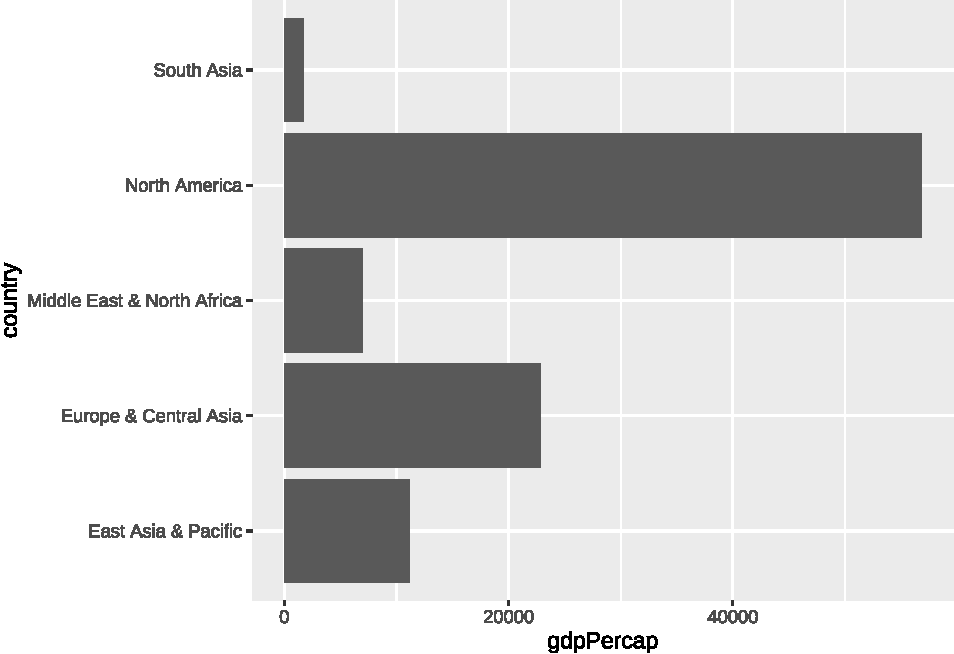
\includegraphics{25-transform_files/figure-latex/unnamed-chunk-41-1.pdf}

一応、なにか描けましたが、どうも、すごく点の数が多いですね。それと、欠損値もたくさんあるようです。また、gdpPercap でみると、値が小さいところに固まってあるようです。

まずは、すべての年について、値を使っていますから、2022 年に限ってみましょう。

\begin{Shaded}
\begin{Highlighting}[]
\NormalTok{df\_wdi3c }\SpecialCharTok{|\textgreater{}} \FunctionTok{filter}\NormalTok{(year }\SpecialCharTok{==} \StringTok{"2022"}\NormalTok{) }\SpecialCharTok{|\textgreater{}}
  \FunctionTok{ggplot}\NormalTok{(}\FunctionTok{aes}\NormalTok{(gdpPercap, lifeExp)) }\SpecialCharTok{+} \FunctionTok{geom\_point}\NormalTok{()}
\CommentTok{\#\textgreater{} Warning: Removed 216 rows containing missing values}
\CommentTok{\#\textgreater{} (\textasciigrave{}geom\_point()\textasciigrave{}).}
\end{Highlighting}
\end{Shaded}

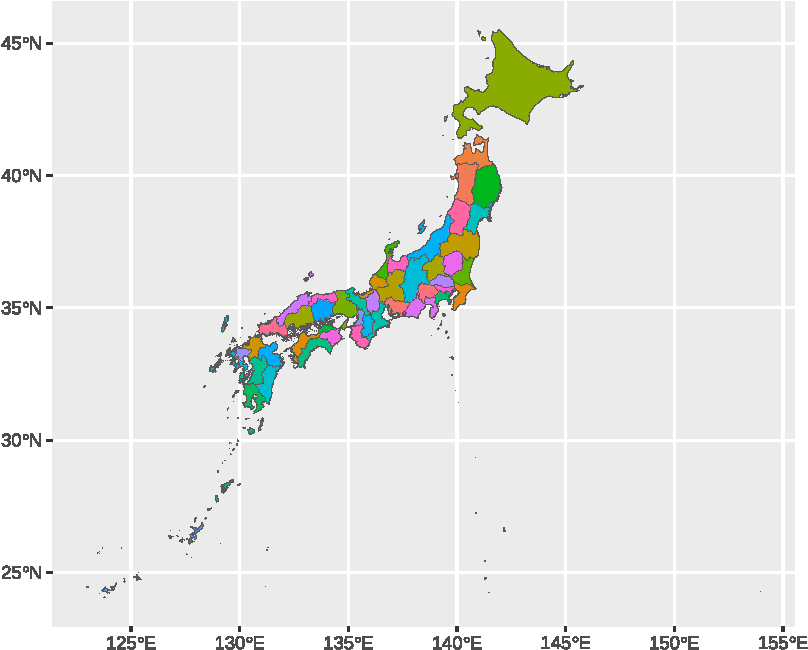
\includegraphics{25-transform_files/figure-latex/unnamed-chunk-42-1.pdf}

どうも、何も現れません。2021 年ならどうでしょうか。

\begin{Shaded}
\begin{Highlighting}[]
\NormalTok{df\_wdi3c }\SpecialCharTok{|\textgreater{}} \FunctionTok{filter}\NormalTok{(year }\SpecialCharTok{==} \DecValTok{2021}\NormalTok{) }\SpecialCharTok{|\textgreater{}}
  \FunctionTok{ggplot}\NormalTok{(}\FunctionTok{aes}\NormalTok{(gdpPercap, lifeExp)) }\SpecialCharTok{+} \FunctionTok{geom\_point}\NormalTok{()}
\CommentTok{\#\textgreater{} Warning: Removed 22 rows containing missing values}
\CommentTok{\#\textgreater{} (\textasciigrave{}geom\_point()\textasciigrave{}).}
\end{Highlighting}
\end{Shaded}

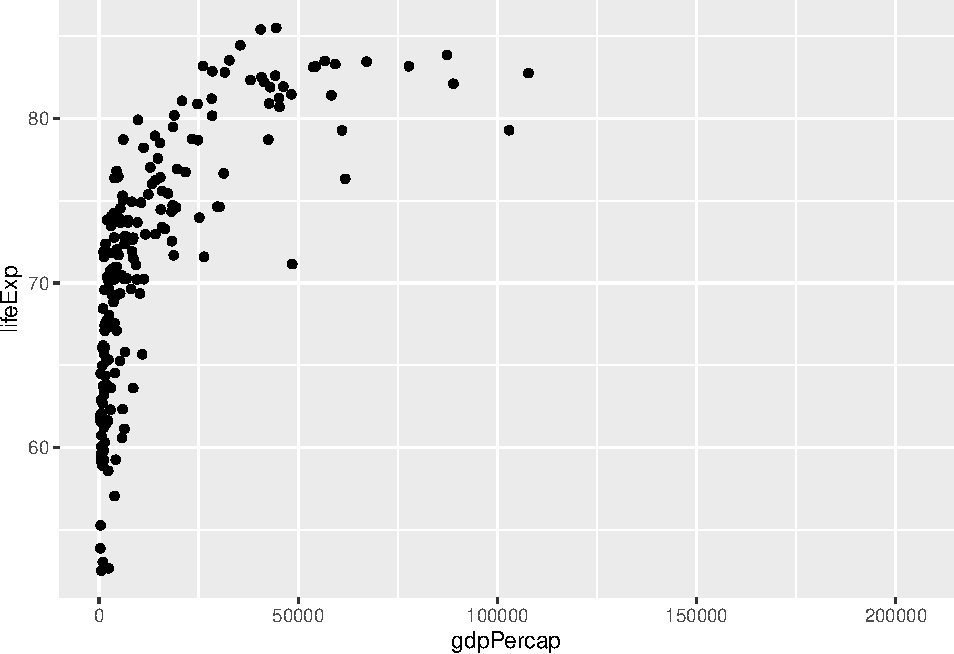
\includegraphics{25-transform_files/figure-latex/unnamed-chunk-43-1.pdf}

データがない国もあるようですが、どうやら表示されました。データがない国は、削除しておいたり region を 色で表したり、人口を、点の大きさで表したり、gdpPercap を log10 をとって、値を修正して表すなども可能ですが、それは、可視化の項目で学びます。

\begin{Shaded}
\begin{Highlighting}[]
\NormalTok{df\_wdi3c }\SpecialCharTok{|\textgreater{}} \FunctionTok{filter}\NormalTok{(year }\SpecialCharTok{==} \DecValTok{2021}\NormalTok{) }\SpecialCharTok{|\textgreater{}} \FunctionTok{drop\_na}\NormalTok{(lifeExp, gdpPercap) }\SpecialCharTok{|\textgreater{}}
  \FunctionTok{ggplot}\NormalTok{(}\FunctionTok{aes}\NormalTok{(gdpPercap, lifeExp, }\AttributeTok{color =}\NormalTok{ region, }\AttributeTok{size =}\NormalTok{ pop)) }\SpecialCharTok{+} 
  \FunctionTok{geom\_point}\NormalTok{() }\SpecialCharTok{+} \FunctionTok{scale\_x\_log10}\NormalTok{()}
\end{Highlighting}
\end{Shaded}

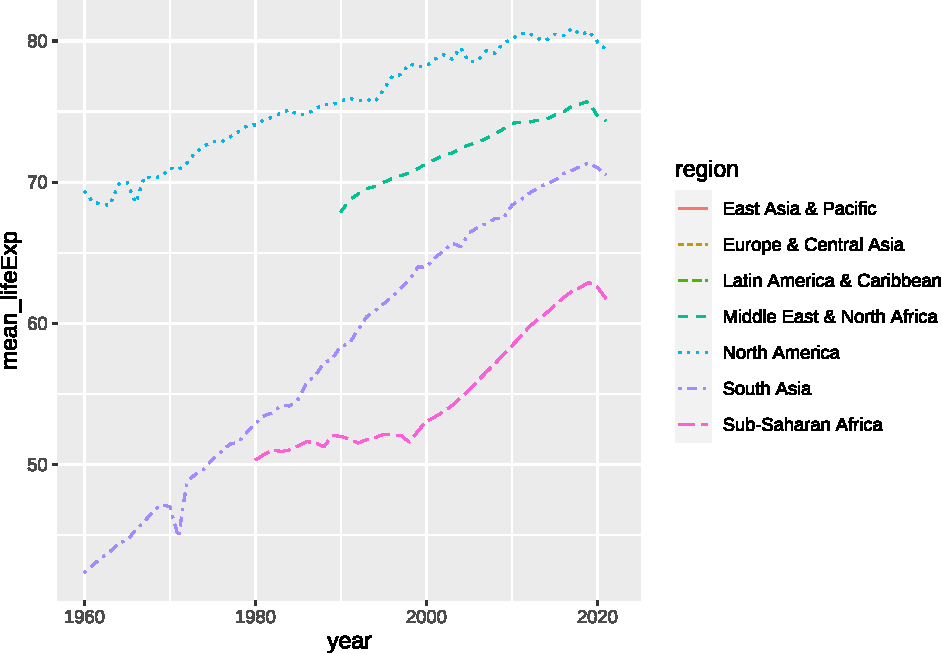
\includegraphics{25-transform_files/figure-latex/unnamed-chunk-44-1.pdf}

こうしてみると、gdpPercap が大きい国ほど、lifeExp も大きい傾向があることも見えますね。

ここまでは、\texttt{select} と、\texttt{filter} を使ってきましたが、\texttt{arrange}、\texttt{mutate}、\texttt{group\_by} や、\texttt{summarize} も使ってみましょう。

まず、gdpPercap は一人当たりの GDP でしたから、この値に、pop 人口をかければ、原理的には、GDP が得られることになります。(さまざまな基準がありますから、詳細は、調べてください。)順番を、入れ替えて、year の次に、gdp がくるようにしておきます。他にも、year の後に置くようにとの指示もできます。Help で確認してください。例も載っています。また、掛け算は、* を使います。これを、df\_wdi4c としておきましょう。また、year が順番になっていないのが気になりますから、大きい順に並べ替えておきましょう。

\begin{Shaded}
\begin{Highlighting}[]
\NormalTok{df\_wdi4c }\OtherTok{\textless{}{-}}\NormalTok{ df\_wdi3c }\SpecialCharTok{|\textgreater{}} \FunctionTok{mutate}\NormalTok{(}\AttributeTok{gdp =}\NormalTok{ pop}\SpecialCharTok{*}\NormalTok{gdpPercap) }\SpecialCharTok{|\textgreater{}} 
  \FunctionTok{select}\NormalTok{(}\DecValTok{1}\NormalTok{,}\DecValTok{2}\NormalTok{,}\DecValTok{3}\NormalTok{,}\DecValTok{9}\NormalTok{,}\DecValTok{4}\NormalTok{,}\DecValTok{5}\NormalTok{,}\DecValTok{6}\NormalTok{,}\DecValTok{7}\NormalTok{,}\DecValTok{8}\NormalTok{) }\SpecialCharTok{|\textgreater{}} \FunctionTok{arrange}\NormalTok{(country, }\FunctionTok{desc}\NormalTok{(year))}
\NormalTok{df\_wdi4c}
\CommentTok{\#\textgreater{} \# A tibble: 13,608 x 9}
\CommentTok{\#\textgreater{}    country     iso2c  year      gdp lifeExp    pop gdpPercap}
\CommentTok{\#\textgreater{}    \textless{}chr\textgreater{}       \textless{}chr\textgreater{} \textless{}dbl\textgreater{}    \textless{}dbl\textgreater{}   \textless{}dbl\textgreater{}  \textless{}dbl\textgreater{}     \textless{}dbl\textgreater{}}
\CommentTok{\#\textgreater{}  1 Afghanistan AF     2022 NA          NA   4.11e7       NA }
\CommentTok{\#\textgreater{}  2 Afghanistan AF     2021  1.71e10    62.0 4.01e7      426.}
\CommentTok{\#\textgreater{}  3 Afghanistan AF     2020  2.16e10    62.6 3.90e7      553.}
\CommentTok{\#\textgreater{}  4 Afghanistan AF     2019  2.21e10    63.6 3.78e7      584.}
\CommentTok{\#\textgreater{}  5 Afghanistan AF     2018  2.12e10    63.1 3.67e7      579.}
\CommentTok{\#\textgreater{}  6 Afghanistan AF     2017  2.10e10    63.0 3.56e7      589.}
\CommentTok{\#\textgreater{}  7 Afghanistan AF     2016  2.05e10    63.1 3.46e7      590.}
\CommentTok{\#\textgreater{}  8 Afghanistan AF     2015  2.00e10    62.7 3.38e7      592.}
\CommentTok{\#\textgreater{}  9 Afghanistan AF     2014  1.97e10    62.5 3.27e7      603.}
\CommentTok{\#\textgreater{} 10 Afghanistan AF     2013  1.92e10    62.4 3.15e7      608.}
\CommentTok{\#\textgreater{} \# i 13,598 more rows}
\CommentTok{\#\textgreater{} \# i 2 more variables: income \textless{}chr\textgreater{}, region \textless{}chr\textgreater{}}
\end{Highlighting}
\end{Shaded}

\begin{Shaded}
\begin{Highlighting}[]
\NormalTok{df\_wdi3c }\SpecialCharTok{|\textgreater{}} \FunctionTok{mutate}\NormalTok{(}\AttributeTok{gdp =}\NormalTok{ pop}\SpecialCharTok{*}\NormalTok{gdpPercap, }\AttributeTok{.after =}\NormalTok{ year) }\SpecialCharTok{|\textgreater{}} 
  \FunctionTok{arrange}\NormalTok{(country, }\FunctionTok{desc}\NormalTok{(year))}
\CommentTok{\#\textgreater{} \# A tibble: 13,608 x 9}
\CommentTok{\#\textgreater{}    country     iso2c  year      gdp lifeExp    pop gdpPercap}
\CommentTok{\#\textgreater{}    \textless{}chr\textgreater{}       \textless{}chr\textgreater{} \textless{}dbl\textgreater{}    \textless{}dbl\textgreater{}   \textless{}dbl\textgreater{}  \textless{}dbl\textgreater{}     \textless{}dbl\textgreater{}}
\CommentTok{\#\textgreater{}  1 Afghanistan AF     2022 NA          NA   4.11e7       NA }
\CommentTok{\#\textgreater{}  2 Afghanistan AF     2021  1.71e10    62.0 4.01e7      426.}
\CommentTok{\#\textgreater{}  3 Afghanistan AF     2020  2.16e10    62.6 3.90e7      553.}
\CommentTok{\#\textgreater{}  4 Afghanistan AF     2019  2.21e10    63.6 3.78e7      584.}
\CommentTok{\#\textgreater{}  5 Afghanistan AF     2018  2.12e10    63.1 3.67e7      579.}
\CommentTok{\#\textgreater{}  6 Afghanistan AF     2017  2.10e10    63.0 3.56e7      589.}
\CommentTok{\#\textgreater{}  7 Afghanistan AF     2016  2.05e10    63.1 3.46e7      590.}
\CommentTok{\#\textgreater{}  8 Afghanistan AF     2015  2.00e10    62.7 3.38e7      592.}
\CommentTok{\#\textgreater{}  9 Afghanistan AF     2014  1.97e10    62.5 3.27e7      603.}
\CommentTok{\#\textgreater{} 10 Afghanistan AF     2013  1.92e10    62.4 3.15e7      608.}
\CommentTok{\#\textgreater{} \# i 13,598 more rows}
\CommentTok{\#\textgreater{} \# i 2 more variables: income \textless{}chr\textgreater{}, region \textless{}chr\textgreater{}}
\end{Highlighting}
\end{Shaded}

2022 年のデータはあまりないようですから、2021 年の GDP の大きい順に並べてみましょう。gdp が 2.052946e13 などと書かれているのは、指数表示(Scientific Notation)で、e3 は、1000 千、e6 は、1,000,000 百万、e9 は、1,000,000,000 千億、e12 は、1,000,000,000,000 超です。つまり、アメリカの GDP は、だいたい、20兆ドル、日本は、4.5兆ドルと言ったところです。

\begin{Shaded}
\begin{Highlighting}[]
\NormalTok{df\_wdi4c }\SpecialCharTok{|\textgreater{}} \FunctionTok{filter}\NormalTok{(year }\SpecialCharTok{==} \DecValTok{2021}\NormalTok{) }\SpecialCharTok{|\textgreater{}} \FunctionTok{arrange}\NormalTok{(}\FunctionTok{desc}\NormalTok{(gdp))}
\CommentTok{\#\textgreater{} \# A tibble: 216 x 9}
\CommentTok{\#\textgreater{}    country      iso2c  year     gdp lifeExp    pop gdpPercap}
\CommentTok{\#\textgreater{}    \textless{}chr\textgreater{}        \textless{}chr\textgreater{} \textless{}dbl\textgreater{}   \textless{}dbl\textgreater{}   \textless{}dbl\textgreater{}  \textless{}dbl\textgreater{}     \textless{}dbl\textgreater{}}
\CommentTok{\#\textgreater{}  1 United Stat\textasciitilde{} US     2021 2.05e13    76.3 3.32e8    61830.}
\CommentTok{\#\textgreater{}  2 China        CN     2021 1.59e13    78.2 1.41e9    11223.}
\CommentTok{\#\textgreater{}  3 Japan        JP     2021 4.46e12    84.4 1.26e8    35508.}
\CommentTok{\#\textgreater{}  4 Germany      DE     2021 3.55e12    80.9 8.32e7    42726.}
\CommentTok{\#\textgreater{}  5 United King\textasciitilde{} GB     2021 3.04e12    80.7 6.70e7    45334.}
\CommentTok{\#\textgreater{}  6 India        IN     2021 2.76e12    67.2 1.41e9     1962.}
\CommentTok{\#\textgreater{}  7 France       FR     2021 2.58e12    82.3 6.77e7    38046.}
\CommentTok{\#\textgreater{}  8 Italy        IT     2021 1.87e12    82.8 5.91e7    31601.}
\CommentTok{\#\textgreater{}  9 Brazil       BR     2021 1.85e12    72.8 2.14e8     8622.}
\CommentTok{\#\textgreater{} 10 Korea, Rep.  KR     2021 1.69e12    83.5 5.17e7    32731.}
\CommentTok{\#\textgreater{} \# i 206 more rows}
\CommentTok{\#\textgreater{} \# i 2 more variables: income \textless{}chr\textgreater{}, region \textless{}chr\textgreater{}}
\end{Highlighting}
\end{Shaded}

地域ごとの平均寿命を求めてみましょう。

\begin{Shaded}
\begin{Highlighting}[]
\NormalTok{df\_wdi4c }\SpecialCharTok{|\textgreater{}} \FunctionTok{drop\_na}\NormalTok{(lifeExp) }\SpecialCharTok{|\textgreater{}} 
  \FunctionTok{group\_by}\NormalTok{(region) }\SpecialCharTok{|\textgreater{}} \FunctionTok{summarize}\NormalTok{(}\AttributeTok{lifeexpregion =} \FunctionTok{mean}\NormalTok{(lifeExp)) }\SpecialCharTok{|\textgreater{}}
  \FunctionTok{arrange}\NormalTok{(}\FunctionTok{desc}\NormalTok{(lifeexpregion))}
\CommentTok{\#\textgreater{} \# A tibble: 7 x 2}
\CommentTok{\#\textgreater{}   region                     lifeexpregion}
\CommentTok{\#\textgreater{}   \textless{}chr\textgreater{}                              \textless{}dbl\textgreater{}}
\CommentTok{\#\textgreater{} 1 North America                       75.6}
\CommentTok{\#\textgreater{} 2 Europe \& Central Asia               72.2}
\CommentTok{\#\textgreater{} 3 Latin America \& Caribbean           68.3}
\CommentTok{\#\textgreater{} 4 Middle East \& North Africa          66.2}
\CommentTok{\#\textgreater{} 5 East Asia \& Pacific                 66.0}
\CommentTok{\#\textgreater{} 6 South Asia                          58.1}
\CommentTok{\#\textgreater{} 7 Sub{-}Saharan Africa                  52.1}
\end{Highlighting}
\end{Shaded}

income でも計算してみましょう。

\begin{Shaded}
\begin{Highlighting}[]
\NormalTok{df\_wdi4c }\SpecialCharTok{|\textgreater{}} \FunctionTok{drop\_na}\NormalTok{(lifeExp) }\SpecialCharTok{|\textgreater{}} 
  \FunctionTok{group\_by}\NormalTok{(income) }\SpecialCharTok{|\textgreater{}} \FunctionTok{summarize}\NormalTok{(}\AttributeTok{lifeexpincome =} \FunctionTok{mean}\NormalTok{(lifeExp)) }\SpecialCharTok{|\textgreater{}}
  \FunctionTok{arrange}\NormalTok{(}\FunctionTok{desc}\NormalTok{(lifeexpincome))}
\CommentTok{\#\textgreater{} \# A tibble: 5 x 2}
\CommentTok{\#\textgreater{}   income              lifeexpincome}
\CommentTok{\#\textgreater{}   \textless{}chr\textgreater{}                       \textless{}dbl\textgreater{}}
\CommentTok{\#\textgreater{} 1 High income                  73.4}
\CommentTok{\#\textgreater{} 2 Not classified               69.2}
\CommentTok{\#\textgreater{} 3 Upper middle income          66.4}
\CommentTok{\#\textgreater{} 4 Lower middle income          58.8}
\CommentTok{\#\textgreater{} 5 Low income                   50.1}
\end{Highlighting}
\end{Shaded}

ある年の値がないためにグラフがかけない場合もあります。各指標の年毎のデータがどれぐらいあるかみてみましょう。\texttt{is.na(x)} は、x が NA なら TRUE (値は 1)、x が NA でなければ、FALSE(値は 0)を返します。\texttt{!is.na(x)} はその否定ですから、逆になります。そこで、たとえば、\texttt{sum(!is.na(gdp))} は、gdp という列(年毎にグループ分けした)の中の、NA ではないものがいくつあるか数えることになります。sum は summation で、合計です。

\begin{Shaded}
\begin{Highlighting}[]
\NormalTok{df\_wdi4c }\SpecialCharTok{|\textgreater{}} \FunctionTok{group\_by}\NormalTok{(year) }\SpecialCharTok{|\textgreater{}} 
  \FunctionTok{summarize}\NormalTok{(}\AttributeTok{gdp\_n =} \FunctionTok{sum}\NormalTok{(}\SpecialCharTok{!}\FunctionTok{is.na}\NormalTok{(gdp)), }\AttributeTok{lifeExp\_n =} \FunctionTok{sum}\NormalTok{(}\SpecialCharTok{!}\FunctionTok{is.na}\NormalTok{(lifeExp)), }\AttributeTok{pop\_n =} \FunctionTok{sum}\NormalTok{(}\SpecialCharTok{!}\FunctionTok{is.na}\NormalTok{(pop)), }\AttributeTok{gdpPercap\_n =} \FunctionTok{sum}\NormalTok{(}\SpecialCharTok{!}\FunctionTok{is.na}\NormalTok{(gdpPercap))) }\SpecialCharTok{|\textgreater{}} \FunctionTok{arrange}\NormalTok{(}\FunctionTok{desc}\NormalTok{(year))}
\CommentTok{\#\textgreater{} \# A tibble: 63 x 5}
\CommentTok{\#\textgreater{}     year gdp\_n lifeExp\_n pop\_n gdpPercap\_n}
\CommentTok{\#\textgreater{}    \textless{}dbl\textgreater{} \textless{}int\textgreater{}     \textless{}int\textgreater{} \textless{}int\textgreater{}       \textless{}int\textgreater{}}
\CommentTok{\#\textgreater{}  1  2022   185         0   216         185}
\CommentTok{\#\textgreater{}  2  2021   201       208   216         201}
\CommentTok{\#\textgreater{}  3  2020   206       208   216         206}
\CommentTok{\#\textgreater{}  4  2019   206       208   216         206}
\CommentTok{\#\textgreater{}  5  2018   206       208   216         206}
\CommentTok{\#\textgreater{}  6  2017   206       209   216         206}
\CommentTok{\#\textgreater{}  7  2016   206       209   216         206}
\CommentTok{\#\textgreater{}  8  2015   209       209   216         209}
\CommentTok{\#\textgreater{}  9  2014   207       209   216         207}
\CommentTok{\#\textgreater{} 10  2013   207       209   216         207}
\CommentTok{\#\textgreater{} \# i 53 more rows}
\end{Highlighting}
\end{Shaded}

\hypertarget{filter}{%
\subsection{\texorpdfstring{\texttt{filter}}{filter}}\label{filter}}

一番上に、国名(country)に、アフガニスタン(Afghanistan) がありましたから、aアフガニスタンのデータを選び、平均寿命(lifeExp: Life Expectancy)の折線グラフ(line graph)を描いてみましょう。まずは、filter で、アフガニスタンのデータを抽出します。スペルに注意してください。コピーをするのが安全かもしれません。フ(line graph)を描いてみましょう。まずは、filter で、アフガニスタンのデータを抽出します。スペルに注意してください。コピーをするのが安全かもしれません。

\texttt{filter(country\ ==\ "Afghanistan")}

特定の値のデータを抽出するには、\texttt{==} を使うのでした。二つの \texttt{=} ですから、間違わないでください。

\begin{Shaded}
\begin{Highlighting}[]
\NormalTok{df\_wdi }\SpecialCharTok{|\textgreater{}} \FunctionTok{filter}\NormalTok{(country }\SpecialCharTok{==} \StringTok{"Afghanistan"}\NormalTok{)}
\CommentTok{\#\textgreater{} \# A tibble: 63 x 7}
\CommentTok{\#\textgreater{}    country     iso2c iso3c  year lifeExp      pop gdpPercap}
\CommentTok{\#\textgreater{}    \textless{}chr\textgreater{}       \textless{}chr\textgreater{} \textless{}chr\textgreater{} \textless{}dbl\textgreater{}   \textless{}dbl\textgreater{}    \textless{}dbl\textgreater{}     \textless{}dbl\textgreater{}}
\CommentTok{\#\textgreater{}  1 Afghanistan AF    AFG    1960    32.5  8622466        NA}
\CommentTok{\#\textgreater{}  2 Afghanistan AF    AFG    1961    33.1  8790140        NA}
\CommentTok{\#\textgreater{}  3 Afghanistan AF    AFG    1962    33.5  8969047        NA}
\CommentTok{\#\textgreater{}  4 Afghanistan AF    AFG    1963    34.0  9157465        NA}
\CommentTok{\#\textgreater{}  5 Afghanistan AF    AFG    1964    34.5  9355514        NA}
\CommentTok{\#\textgreater{}  6 Afghanistan AF    AFG    1965    35.0  9565147        NA}
\CommentTok{\#\textgreater{}  7 Afghanistan AF    AFG    1966    35.5  9783147        NA}
\CommentTok{\#\textgreater{}  8 Afghanistan AF    AFG    1967    35.9 10010030        NA}
\CommentTok{\#\textgreater{}  9 Afghanistan AF    AFG    1968    36.4 10247780        NA}
\CommentTok{\#\textgreater{} 10 Afghanistan AF    AFG    1969    36.9 10494489        NA}
\CommentTok{\#\textgreater{} \# i 53 more rows}
\end{Highlighting}
\end{Shaded}

確認できましたか。

折線グラフを書きます。この場合は、GEOM は、\texttt{geom\_line} です。

\begin{Shaded}
\begin{Highlighting}[]
\NormalTok{df\_wdi }\SpecialCharTok{|\textgreater{}} \FunctionTok{filter}\NormalTok{(country }\SpecialCharTok{==} \StringTok{"Afghanistan"}\NormalTok{) }\SpecialCharTok{\%\textgreater{}\%}
  \FunctionTok{ggplot}\NormalTok{(}\FunctionTok{aes}\NormalTok{(}\AttributeTok{x =}\NormalTok{ year, }\AttributeTok{y =}\NormalTok{ lifeExp)) }\SpecialCharTok{+} \FunctionTok{geom\_line}\NormalTok{()}
\CommentTok{\#\textgreater{} Warning: Removed 1 row containing missing values}
\CommentTok{\#\textgreater{} (\textasciigrave{}geom\_line()\textasciigrave{}).}
\end{Highlighting}
\end{Shaded}

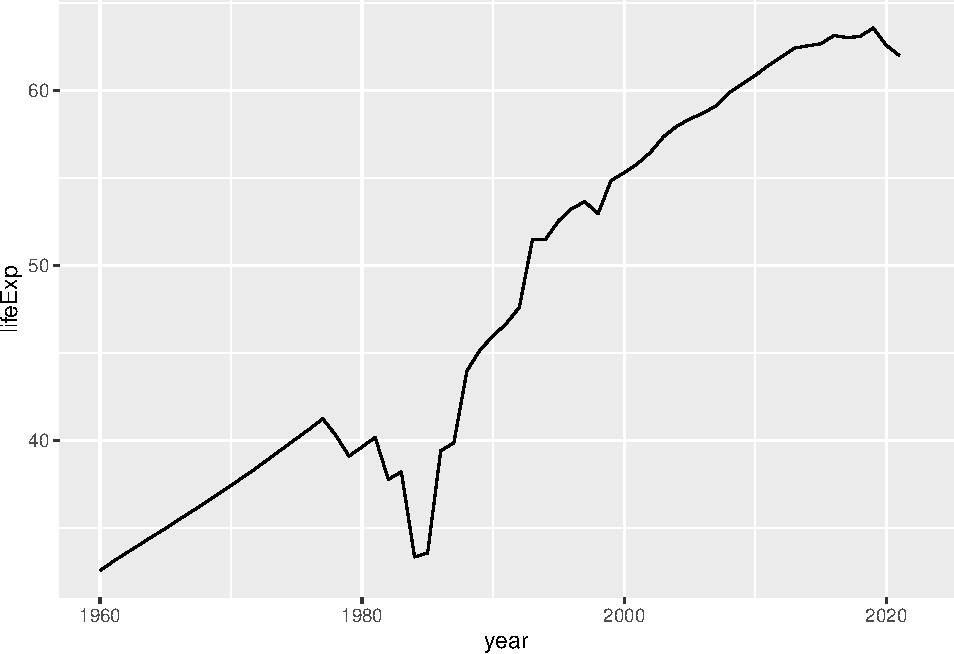
\includegraphics{25-transform_files/figure-latex/unnamed-chunk-52-1.pdf}

アフガニスタンでは 1952年 の誕生時の平均寿命(life expectancy at birth)は 30歳以下 (28.8歳)でした。2007年でも50歳以下(48.8 歳)のようですね。改善されていることも確かです。

アフガニスタンと日本両方を抽出してみましょう。そのときは、 \texttt{country\ \%in\%\ c("Afghanistan",\ "Japan")} とします。

\begin{Shaded}
\begin{Highlighting}[]
\NormalTok{df\_wdi }\SpecialCharTok{\%\textgreater{}\%} \FunctionTok{filter}\NormalTok{(country }\SpecialCharTok{\%in\%} \FunctionTok{c}\NormalTok{(}\StringTok{"Afghanistan"}\NormalTok{, }\StringTok{"Japan"}\NormalTok{))}
\CommentTok{\#\textgreater{} \# A tibble: 126 x 7}
\CommentTok{\#\textgreater{}    country     iso2c iso3c  year lifeExp      pop gdpPercap}
\CommentTok{\#\textgreater{}    \textless{}chr\textgreater{}       \textless{}chr\textgreater{} \textless{}chr\textgreater{} \textless{}dbl\textgreater{}   \textless{}dbl\textgreater{}    \textless{}dbl\textgreater{}     \textless{}dbl\textgreater{}}
\CommentTok{\#\textgreater{}  1 Afghanistan AF    AFG    1960    32.5  8622466        NA}
\CommentTok{\#\textgreater{}  2 Afghanistan AF    AFG    1961    33.1  8790140        NA}
\CommentTok{\#\textgreater{}  3 Afghanistan AF    AFG    1962    33.5  8969047        NA}
\CommentTok{\#\textgreater{}  4 Afghanistan AF    AFG    1963    34.0  9157465        NA}
\CommentTok{\#\textgreater{}  5 Afghanistan AF    AFG    1964    34.5  9355514        NA}
\CommentTok{\#\textgreater{}  6 Afghanistan AF    AFG    1965    35.0  9565147        NA}
\CommentTok{\#\textgreater{}  7 Afghanistan AF    AFG    1966    35.5  9783147        NA}
\CommentTok{\#\textgreater{}  8 Afghanistan AF    AFG    1967    35.9 10010030        NA}
\CommentTok{\#\textgreater{}  9 Afghanistan AF    AFG    1968    36.4 10247780        NA}
\CommentTok{\#\textgreater{} 10 Afghanistan AF    AFG    1969    36.9 10494489        NA}
\CommentTok{\#\textgreater{} \# i 116 more rows}
\end{Highlighting}
\end{Shaded}

グラフにしてみましょう。今度は、区別のため、\texttt{color\ =\ country} を追加します。すると、線が違う色で表示されます。詳しくは、視覚化を参照してください。

\begin{Shaded}
\begin{Highlighting}[]
\NormalTok{df\_wdi }\SpecialCharTok{\%\textgreater{}\%} \FunctionTok{filter}\NormalTok{(country }\SpecialCharTok{\%in\%} \FunctionTok{c}\NormalTok{(}\StringTok{"Afghanistan"}\NormalTok{, }\StringTok{"Japan"}\NormalTok{)) }\SpecialCharTok{\%\textgreater{}\%}
  \FunctionTok{ggplot}\NormalTok{(}\FunctionTok{aes}\NormalTok{(}\AttributeTok{x =}\NormalTok{ year, }\AttributeTok{y =}\NormalTok{ lifeExp, }\AttributeTok{color =}\NormalTok{ country)) }\SpecialCharTok{+} \FunctionTok{geom\_line}\NormalTok{()}
\CommentTok{\#\textgreater{} Warning: Removed 2 rows containing missing values}
\CommentTok{\#\textgreater{} (\textasciigrave{}geom\_line()\textasciigrave{}).}
\end{Highlighting}
\end{Shaded}

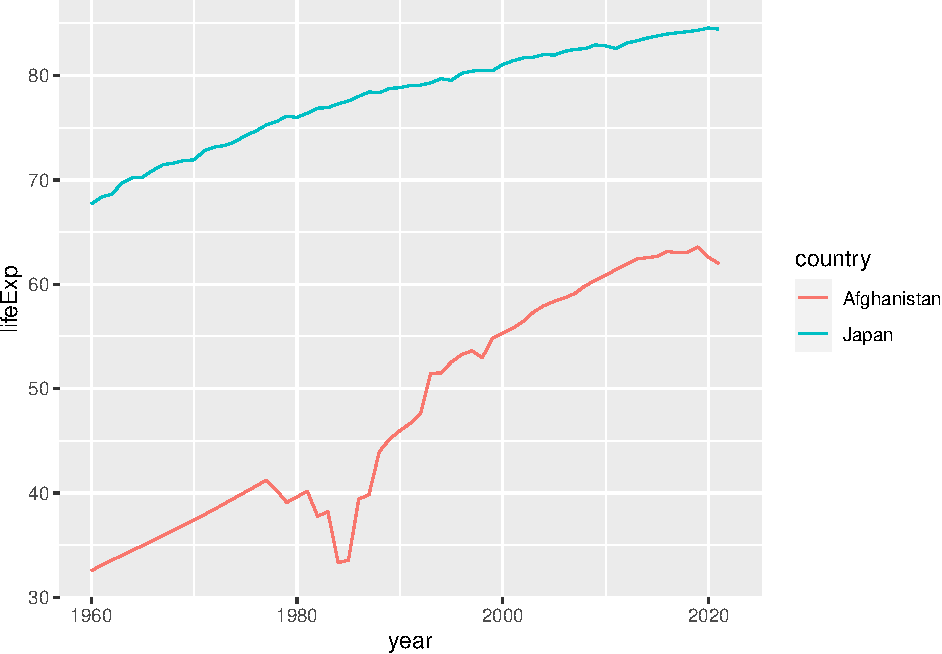
\includegraphics{25-transform_files/figure-latex/unnamed-chunk-54-1.pdf}

どのような発見がありますか。かならず書き留めておいてください。

他の国についても調べるときは、国のリストがあるとよいので、 \texttt{unique(df\_gm\$country)} とすると、リストが得られます。\texttt{distinct(country)} で、異なる国を選択してから、その部分をベクトルとして出力することもできます。

\begin{Shaded}
\begin{Highlighting}[]
\NormalTok{df\_wdi }\SpecialCharTok{\%\textgreater{}\%} \FunctionTok{distinct}\NormalTok{(country) }\SpecialCharTok{\%\textgreater{}\%} \FunctionTok{pull}\NormalTok{()}
\CommentTok{\#\textgreater{}   [1] "Afghanistan"                                         }
\CommentTok{\#\textgreater{}   [2] "Africa Eastern and Southern"                         }
\CommentTok{\#\textgreater{}   [3] "Africa Western and Central"                          }
\CommentTok{\#\textgreater{}   [4] "Albania"                                             }
\CommentTok{\#\textgreater{}   [5] "Algeria"                                             }
\CommentTok{\#\textgreater{}   [6] "American Samoa"                                      }
\CommentTok{\#\textgreater{}   [7] "Andorra"                                             }
\CommentTok{\#\textgreater{}   [8] "Angola"                                              }
\CommentTok{\#\textgreater{}   [9] "Antigua and Barbuda"                                 }
\CommentTok{\#\textgreater{}  [10] "Arab World"                                          }
\CommentTok{\#\textgreater{}  [11] "Argentina"                                           }
\CommentTok{\#\textgreater{}  [12] "Armenia"                                             }
\CommentTok{\#\textgreater{}  [13] "Aruba"                                               }
\CommentTok{\#\textgreater{}  [14] "Australia"                                           }
\CommentTok{\#\textgreater{}  [15] "Austria"                                             }
\CommentTok{\#\textgreater{}  [16] "Azerbaijan"                                          }
\CommentTok{\#\textgreater{}  [17] "Bahamas, The"                                        }
\CommentTok{\#\textgreater{}  [18] "Bahrain"                                             }
\CommentTok{\#\textgreater{}  [19] "Bangladesh"                                          }
\CommentTok{\#\textgreater{}  [20] "Barbados"                                            }
\CommentTok{\#\textgreater{}  [21] "Belarus"                                             }
\CommentTok{\#\textgreater{}  [22] "Belgium"                                             }
\CommentTok{\#\textgreater{}  [23] "Belize"                                              }
\CommentTok{\#\textgreater{}  [24] "Benin"                                               }
\CommentTok{\#\textgreater{}  [25] "Bermuda"                                             }
\CommentTok{\#\textgreater{}  [26] "Bhutan"                                              }
\CommentTok{\#\textgreater{}  [27] "Bolivia"                                             }
\CommentTok{\#\textgreater{}  [28] "Bosnia and Herzegovina"                              }
\CommentTok{\#\textgreater{}  [29] "Botswana"                                            }
\CommentTok{\#\textgreater{}  [30] "Brazil"                                              }
\CommentTok{\#\textgreater{}  [31] "British Virgin Islands"                              }
\CommentTok{\#\textgreater{}  [32] "Brunei Darussalam"                                   }
\CommentTok{\#\textgreater{}  [33] "Bulgaria"                                            }
\CommentTok{\#\textgreater{}  [34] "Burkina Faso"                                        }
\CommentTok{\#\textgreater{}  [35] "Burundi"                                             }
\CommentTok{\#\textgreater{}  [36] "Cabo Verde"                                          }
\CommentTok{\#\textgreater{}  [37] "Cambodia"                                            }
\CommentTok{\#\textgreater{}  [38] "Cameroon"                                            }
\CommentTok{\#\textgreater{}  [39] "Canada"                                              }
\CommentTok{\#\textgreater{}  [40] "Caribbean small states"                              }
\CommentTok{\#\textgreater{}  [41] "Cayman Islands"                                      }
\CommentTok{\#\textgreater{}  [42] "Central African Republic"                            }
\CommentTok{\#\textgreater{}  [43] "Central Europe and the Baltics"                      }
\CommentTok{\#\textgreater{}  [44] "Chad"                                                }
\CommentTok{\#\textgreater{}  [45] "Channel Islands"                                     }
\CommentTok{\#\textgreater{}  [46] "Chile"                                               }
\CommentTok{\#\textgreater{}  [47] "China"                                               }
\CommentTok{\#\textgreater{}  [48] "Colombia"                                            }
\CommentTok{\#\textgreater{}  [49] "Comoros"                                             }
\CommentTok{\#\textgreater{}  [50] "Congo, Dem. Rep."                                    }
\CommentTok{\#\textgreater{}  [51] "Congo, Rep."                                         }
\CommentTok{\#\textgreater{}  [52] "Costa Rica"                                          }
\CommentTok{\#\textgreater{}  [53] "Cote d\textquotesingle{}Ivoire"                                       }
\CommentTok{\#\textgreater{}  [54] "Croatia"                                             }
\CommentTok{\#\textgreater{}  [55] "Cuba"                                                }
\CommentTok{\#\textgreater{}  [56] "Curacao"                                             }
\CommentTok{\#\textgreater{}  [57] "Cyprus"                                              }
\CommentTok{\#\textgreater{}  [58] "Czechia"                                             }
\CommentTok{\#\textgreater{}  [59] "Denmark"                                             }
\CommentTok{\#\textgreater{}  [60] "Djibouti"                                            }
\CommentTok{\#\textgreater{}  [61] "Dominica"                                            }
\CommentTok{\#\textgreater{}  [62] "Dominican Republic"                                  }
\CommentTok{\#\textgreater{}  [63] "Early{-}demographic dividend"                          }
\CommentTok{\#\textgreater{}  [64] "East Asia \& Pacific"                                 }
\CommentTok{\#\textgreater{}  [65] "East Asia \& Pacific (excluding high income)"         }
\CommentTok{\#\textgreater{}  [66] "East Asia \& Pacific (IDA \& IBRD countries)"          }
\CommentTok{\#\textgreater{}  [67] "Ecuador"                                             }
\CommentTok{\#\textgreater{}  [68] "Egypt, Arab Rep."                                    }
\CommentTok{\#\textgreater{}  [69] "El Salvador"                                         }
\CommentTok{\#\textgreater{}  [70] "Equatorial Guinea"                                   }
\CommentTok{\#\textgreater{}  [71] "Eritrea"                                             }
\CommentTok{\#\textgreater{}  [72] "Estonia"                                             }
\CommentTok{\#\textgreater{}  [73] "Eswatini"                                            }
\CommentTok{\#\textgreater{}  [74] "Ethiopia"                                            }
\CommentTok{\#\textgreater{}  [75] "Euro area"                                           }
\CommentTok{\#\textgreater{}  [76] "Europe \& Central Asia"                               }
\CommentTok{\#\textgreater{}  [77] "Europe \& Central Asia (excluding high income)"       }
\CommentTok{\#\textgreater{}  [78] "Europe \& Central Asia (IDA \& IBRD countries)"        }
\CommentTok{\#\textgreater{}  [79] "European Union"                                      }
\CommentTok{\#\textgreater{}  [80] "Faroe Islands"                                       }
\CommentTok{\#\textgreater{}  [81] "Fiji"                                                }
\CommentTok{\#\textgreater{}  [82] "Finland"                                             }
\CommentTok{\#\textgreater{}  [83] "Fragile and conflict affected situations"            }
\CommentTok{\#\textgreater{}  [84] "France"                                              }
\CommentTok{\#\textgreater{}  [85] "French Polynesia"                                    }
\CommentTok{\#\textgreater{}  [86] "Gabon"                                               }
\CommentTok{\#\textgreater{}  [87] "Gambia, The"                                         }
\CommentTok{\#\textgreater{}  [88] "Georgia"                                             }
\CommentTok{\#\textgreater{}  [89] "Germany"                                             }
\CommentTok{\#\textgreater{}  [90] "Ghana"                                               }
\CommentTok{\#\textgreater{}  [91] "Gibraltar"                                           }
\CommentTok{\#\textgreater{}  [92] "Greece"                                              }
\CommentTok{\#\textgreater{}  [93] "Greenland"                                           }
\CommentTok{\#\textgreater{}  [94] "Grenada"                                             }
\CommentTok{\#\textgreater{}  [95] "Guam"                                                }
\CommentTok{\#\textgreater{}  [96] "Guatemala"                                           }
\CommentTok{\#\textgreater{}  [97] "Guinea"                                              }
\CommentTok{\#\textgreater{}  [98] "Guinea{-}Bissau"                                       }
\CommentTok{\#\textgreater{}  [99] "Guyana"                                              }
\CommentTok{\#\textgreater{} [100] "Haiti"                                               }
\CommentTok{\#\textgreater{} [101] "Heavily indebted poor countries (HIPC)"              }
\CommentTok{\#\textgreater{} [102] "High income"                                         }
\CommentTok{\#\textgreater{} [103] "Honduras"                                            }
\CommentTok{\#\textgreater{} [104] "Hong Kong SAR, China"                                }
\CommentTok{\#\textgreater{} [105] "Hungary"                                             }
\CommentTok{\#\textgreater{} [106] "IBRD only"                                           }
\CommentTok{\#\textgreater{} [107] "Iceland"                                             }
\CommentTok{\#\textgreater{} [108] "IDA \& IBRD total"                                    }
\CommentTok{\#\textgreater{} [109] "IDA blend"                                           }
\CommentTok{\#\textgreater{} [110] "IDA only"                                            }
\CommentTok{\#\textgreater{} [111] "IDA total"                                           }
\CommentTok{\#\textgreater{} [112] "India"                                               }
\CommentTok{\#\textgreater{} [113] "Indonesia"                                           }
\CommentTok{\#\textgreater{} [114] "Iran, Islamic Rep."                                  }
\CommentTok{\#\textgreater{} [115] "Iraq"                                                }
\CommentTok{\#\textgreater{} [116] "Ireland"                                             }
\CommentTok{\#\textgreater{} [117] "Isle of Man"                                         }
\CommentTok{\#\textgreater{} [118] "Israel"                                              }
\CommentTok{\#\textgreater{} [119] "Italy"                                               }
\CommentTok{\#\textgreater{} [120] "Jamaica"                                             }
\CommentTok{\#\textgreater{} [121] "Japan"                                               }
\CommentTok{\#\textgreater{} [122] "Jordan"                                              }
\CommentTok{\#\textgreater{} [123] "Kazakhstan"                                          }
\CommentTok{\#\textgreater{} [124] "Kenya"                                               }
\CommentTok{\#\textgreater{} [125] "Kiribati"                                            }
\CommentTok{\#\textgreater{} [126] "Korea, Dem. People\textquotesingle{}s Rep."                           }
\CommentTok{\#\textgreater{} [127] "Korea, Rep."                                         }
\CommentTok{\#\textgreater{} [128] "Kosovo"                                              }
\CommentTok{\#\textgreater{} [129] "Kuwait"                                              }
\CommentTok{\#\textgreater{} [130] "Kyrgyz Republic"                                     }
\CommentTok{\#\textgreater{} [131] "Lao PDR"                                             }
\CommentTok{\#\textgreater{} [132] "Late{-}demographic dividend"                           }
\CommentTok{\#\textgreater{} [133] "Latin America \& Caribbean"                           }
\CommentTok{\#\textgreater{} [134] "Latin America \& Caribbean (excluding high income)"   }
\CommentTok{\#\textgreater{} [135] "Latin America \& the Caribbean (IDA \& IBRD countries)"}
\CommentTok{\#\textgreater{} [136] "Latvia"                                              }
\CommentTok{\#\textgreater{} [137] "Least developed countries: UN classification"        }
\CommentTok{\#\textgreater{} [138] "Lebanon"                                             }
\CommentTok{\#\textgreater{} [139] "Lesotho"                                             }
\CommentTok{\#\textgreater{} [140] "Liberia"                                             }
\CommentTok{\#\textgreater{} [141] "Libya"                                               }
\CommentTok{\#\textgreater{} [142] "Liechtenstein"                                       }
\CommentTok{\#\textgreater{} [143] "Lithuania"                                           }
\CommentTok{\#\textgreater{} [144] "Low \& middle income"                                 }
\CommentTok{\#\textgreater{} [145] "Low income"                                          }
\CommentTok{\#\textgreater{} [146] "Lower middle income"                                 }
\CommentTok{\#\textgreater{} [147] "Luxembourg"                                          }
\CommentTok{\#\textgreater{} [148] "Macao SAR, China"                                    }
\CommentTok{\#\textgreater{} [149] "Madagascar"                                          }
\CommentTok{\#\textgreater{} [150] "Malawi"                                              }
\CommentTok{\#\textgreater{} [151] "Malaysia"                                            }
\CommentTok{\#\textgreater{} [152] "Maldives"                                            }
\CommentTok{\#\textgreater{} [153] "Mali"                                                }
\CommentTok{\#\textgreater{} [154] "Malta"                                               }
\CommentTok{\#\textgreater{} [155] "Marshall Islands"                                    }
\CommentTok{\#\textgreater{} [156] "Mauritania"                                          }
\CommentTok{\#\textgreater{} [157] "Mauritius"                                           }
\CommentTok{\#\textgreater{} [158] "Mexico"                                              }
\CommentTok{\#\textgreater{} [159] "Micronesia, Fed. Sts."                               }
\CommentTok{\#\textgreater{} [160] "Middle East \& North Africa"                          }
\CommentTok{\#\textgreater{} [161] "Middle East \& North Africa (excluding high income)"  }
\CommentTok{\#\textgreater{} [162] "Middle East \& North Africa (IDA \& IBRD countries)"   }
\CommentTok{\#\textgreater{} [163] "Middle income"                                       }
\CommentTok{\#\textgreater{} [164] "Moldova"                                             }
\CommentTok{\#\textgreater{} [165] "Monaco"                                              }
\CommentTok{\#\textgreater{} [166] "Mongolia"                                            }
\CommentTok{\#\textgreater{} [167] "Montenegro"                                          }
\CommentTok{\#\textgreater{} [168] "Morocco"                                             }
\CommentTok{\#\textgreater{} [169] "Mozambique"                                          }
\CommentTok{\#\textgreater{} [170] "Myanmar"                                             }
\CommentTok{\#\textgreater{} [171] "Namibia"                                             }
\CommentTok{\#\textgreater{} [172] "Nauru"                                               }
\CommentTok{\#\textgreater{} [173] "Nepal"                                               }
\CommentTok{\#\textgreater{} [174] "Netherlands"                                         }
\CommentTok{\#\textgreater{} [175] "New Caledonia"                                       }
\CommentTok{\#\textgreater{} [176] "New Zealand"                                         }
\CommentTok{\#\textgreater{} [177] "Nicaragua"                                           }
\CommentTok{\#\textgreater{} [178] "Niger"                                               }
\CommentTok{\#\textgreater{} [179] "Nigeria"                                             }
\CommentTok{\#\textgreater{} [180] "North America"                                       }
\CommentTok{\#\textgreater{} [181] "North Macedonia"                                     }
\CommentTok{\#\textgreater{} [182] "Northern Mariana Islands"                            }
\CommentTok{\#\textgreater{} [183] "Norway"                                              }
\CommentTok{\#\textgreater{} [184] "Not classified"                                      }
\CommentTok{\#\textgreater{} [185] "OECD members"                                        }
\CommentTok{\#\textgreater{} [186] "Oman"                                                }
\CommentTok{\#\textgreater{} [187] "Other small states"                                  }
\CommentTok{\#\textgreater{} [188] "Pacific island small states"                         }
\CommentTok{\#\textgreater{} [189] "Pakistan"                                            }
\CommentTok{\#\textgreater{} [190] "Palau"                                               }
\CommentTok{\#\textgreater{} [191] "Panama"                                              }
\CommentTok{\#\textgreater{} [192] "Papua New Guinea"                                    }
\CommentTok{\#\textgreater{} [193] "Paraguay"                                            }
\CommentTok{\#\textgreater{} [194] "Peru"                                                }
\CommentTok{\#\textgreater{} [195] "Philippines"                                         }
\CommentTok{\#\textgreater{} [196] "Poland"                                              }
\CommentTok{\#\textgreater{} [197] "Portugal"                                            }
\CommentTok{\#\textgreater{} [198] "Post{-}demographic dividend"                           }
\CommentTok{\#\textgreater{} [199] "Pre{-}demographic dividend"                            }
\CommentTok{\#\textgreater{} [200] "Puerto Rico"                                         }
\CommentTok{\#\textgreater{} [201] "Qatar"                                               }
\CommentTok{\#\textgreater{} [202] "Romania"                                             }
\CommentTok{\#\textgreater{} [203] "Russian Federation"                                  }
\CommentTok{\#\textgreater{} [204] "Rwanda"                                              }
\CommentTok{\#\textgreater{} [205] "Samoa"                                               }
\CommentTok{\#\textgreater{} [206] "San Marino"                                          }
\CommentTok{\#\textgreater{} [207] "Sao Tome and Principe"                               }
\CommentTok{\#\textgreater{} [208] "Saudi Arabia"                                        }
\CommentTok{\#\textgreater{} [209] "Senegal"                                             }
\CommentTok{\#\textgreater{} [210] "Serbia"                                              }
\CommentTok{\#\textgreater{} [211] "Seychelles"                                          }
\CommentTok{\#\textgreater{} [212] "Sierra Leone"                                        }
\CommentTok{\#\textgreater{} [213] "Singapore"                                           }
\CommentTok{\#\textgreater{} [214] "Sint Maarten (Dutch part)"                           }
\CommentTok{\#\textgreater{} [215] "Slovak Republic"                                     }
\CommentTok{\#\textgreater{} [216] "Slovenia"                                            }
\CommentTok{\#\textgreater{} [217] "Small states"                                        }
\CommentTok{\#\textgreater{} [218] "Solomon Islands"                                     }
\CommentTok{\#\textgreater{} [219] "Somalia"                                             }
\CommentTok{\#\textgreater{} [220] "South Africa"                                        }
\CommentTok{\#\textgreater{} [221] "South Asia"                                          }
\CommentTok{\#\textgreater{} [222] "South Asia (IDA \& IBRD)"                             }
\CommentTok{\#\textgreater{} [223] "South Sudan"                                         }
\CommentTok{\#\textgreater{} [224] "Spain"                                               }
\CommentTok{\#\textgreater{} [225] "Sri Lanka"                                           }
\CommentTok{\#\textgreater{} [226] "St. Kitts and Nevis"                                 }
\CommentTok{\#\textgreater{} [227] "St. Lucia"                                           }
\CommentTok{\#\textgreater{} [228] "St. Martin (French part)"                            }
\CommentTok{\#\textgreater{} [229] "St. Vincent and the Grenadines"                      }
\CommentTok{\#\textgreater{} [230] "Sub{-}Saharan Africa"                                  }
\CommentTok{\#\textgreater{} [231] "Sub{-}Saharan Africa (excluding high income)"          }
\CommentTok{\#\textgreater{} [232] "Sub{-}Saharan Africa (IDA \& IBRD countries)"           }
\CommentTok{\#\textgreater{} [233] "Sudan"                                               }
\CommentTok{\#\textgreater{} [234] "Suriname"                                            }
\CommentTok{\#\textgreater{} [235] "Sweden"                                              }
\CommentTok{\#\textgreater{} [236] "Switzerland"                                         }
\CommentTok{\#\textgreater{} [237] "Syrian Arab Republic"                                }
\CommentTok{\#\textgreater{} [238] "Tajikistan"                                          }
\CommentTok{\#\textgreater{} [239] "Tanzania"                                            }
\CommentTok{\#\textgreater{} [240] "Thailand"                                            }
\CommentTok{\#\textgreater{} [241] "Timor{-}Leste"                                         }
\CommentTok{\#\textgreater{} [242] "Togo"                                                }
\CommentTok{\#\textgreater{} [243] "Tonga"                                               }
\CommentTok{\#\textgreater{} [244] "Trinidad and Tobago"                                 }
\CommentTok{\#\textgreater{} [245] "Tunisia"                                             }
\CommentTok{\#\textgreater{} [246] "Turkiye"                                             }
\CommentTok{\#\textgreater{} [247] "Turkmenistan"                                        }
\CommentTok{\#\textgreater{} [248] "Turks and Caicos Islands"                            }
\CommentTok{\#\textgreater{} [249] "Tuvalu"                                              }
\CommentTok{\#\textgreater{} [250] "Uganda"                                              }
\CommentTok{\#\textgreater{} [251] "Ukraine"                                             }
\CommentTok{\#\textgreater{} [252] "United Arab Emirates"                                }
\CommentTok{\#\textgreater{} [253] "United Kingdom"                                      }
\CommentTok{\#\textgreater{} [254] "United States"                                       }
\CommentTok{\#\textgreater{} [255] "Upper middle income"                                 }
\CommentTok{\#\textgreater{} [256] "Uruguay"                                             }
\CommentTok{\#\textgreater{} [257] "Uzbekistan"                                          }
\CommentTok{\#\textgreater{} [258] "Vanuatu"                                             }
\CommentTok{\#\textgreater{} [259] "Venezuela, RB"                                       }
\CommentTok{\#\textgreater{} [260] "Vietnam"                                             }
\CommentTok{\#\textgreater{} [261] "Virgin Islands (U.S.)"                               }
\CommentTok{\#\textgreater{} [262] "West Bank and Gaza"                                  }
\CommentTok{\#\textgreater{} [263] "World"                                               }
\CommentTok{\#\textgreater{} [264] "Yemen, Rep."                                         }
\CommentTok{\#\textgreater{} [265] "Zambia"                                              }
\CommentTok{\#\textgreater{} [266] "Zimbabwe"}
\end{Highlighting}
\end{Shaded}

このデータには 142 の国のデータがあることがわかりました。

BRICs を選んでみるとどうなるでしょうか。最近は、BRICS として、South Africa を加えることが増えてきているようです。

\begin{Shaded}
\begin{Highlighting}[]
\NormalTok{df\_wdi }\SpecialCharTok{\%\textgreater{}\%} \FunctionTok{filter}\NormalTok{(country }\SpecialCharTok{\%in\%} \FunctionTok{c}\NormalTok{(}\StringTok{"Brazil"}\NormalTok{, }\StringTok{"Russia"}\NormalTok{, }\StringTok{"India"}\NormalTok{, }\StringTok{"China"}\NormalTok{)) }\SpecialCharTok{\%\textgreater{}\%}
  \FunctionTok{ggplot}\NormalTok{(}\FunctionTok{aes}\NormalTok{(}\AttributeTok{x =}\NormalTok{ year, }\AttributeTok{y =}\NormalTok{ lifeExp, }\AttributeTok{color =}\NormalTok{ country)) }\SpecialCharTok{+} \FunctionTok{geom\_line}\NormalTok{()}
\CommentTok{\#\textgreater{} Warning: Removed 3 rows containing missing values}
\CommentTok{\#\textgreater{} (\textasciigrave{}geom\_line()\textasciigrave{}).}
\end{Highlighting}
\end{Shaded}

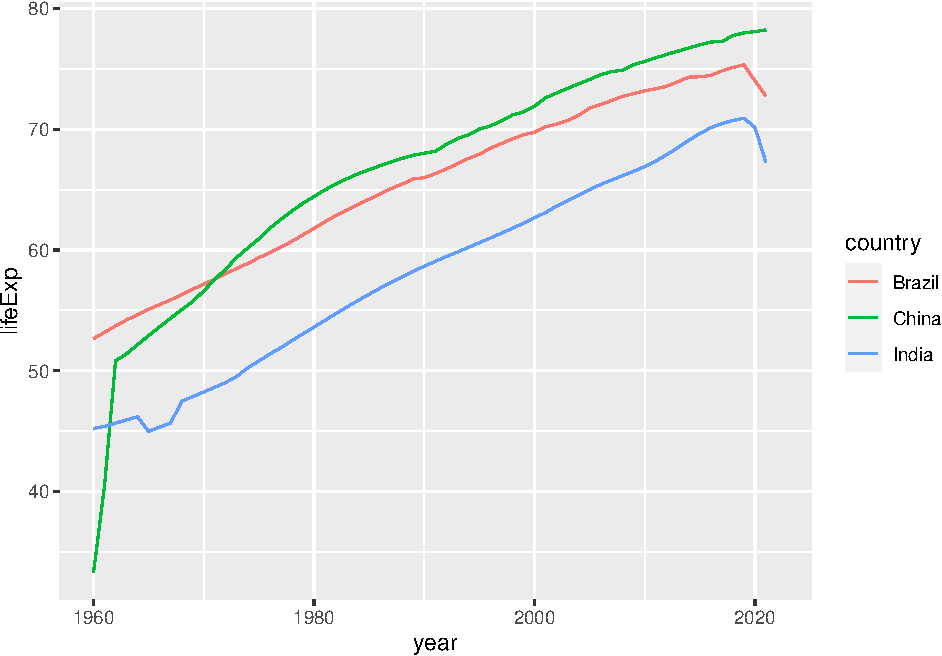
\includegraphics{25-transform_files/figure-latex/unnamed-chunk-56-1.pdf}

ロシアが含まれていないことがわかります。ロシアは、以前は、ソビエト社会主義連邦でしたから、国が変化したものは含まれていないのかもしれません。上の国のリストで見てもありませんね。2007年より新しいデータ、ロシアなども含むデータなど、実際のデータでも見てみたいですね。それは、また後ほど。

\hypertarget{ux7df4ux7fd2-3}{%
\subsection{練習}\label{ux7df4ux7fd2-3}}

\begin{enumerate}
\def\labelenumi{\arabic{enumi}.}
\tightlist
\item
  平均寿命 \texttt{lifeExp} を人口 \texttt{pop} や、一人当たりの GDP \texttt{gdpPercap} に変えて、試してみてください。
\item
  ASEAN (東南アジア諸国連合)ではどうでしょうか。
\end{enumerate}

\begin{itemize}
\item
  Brunei, Cambodia, Indonesia, Laos, Malaysia, Myanmar, Philippines, Singapore.
\item
  このうち幾つの国がこのデータに含まれていますか。
\end{itemize}

\begin{enumerate}
\def\labelenumi{\arabic{enumi}.}
\setcounter{enumi}{2}
\tightlist
\item
  興味のある国をいくつか選んで、三つの指標について調べてみてください。
\end{enumerate}

\hypertarget{group_by-ux3068-summarize}{%
\subsection{\texorpdfstring{\texttt{group\_by} と \texttt{summarize}}{group\_by と summarize}}\label{group_by-ux3068-summarize}}

データには大陸(\texttt{continent} )という変数があります。幾つの大陸があり、それぞれの大陸のいくつ国のデータがこのデータには入っているでしょうか。

それぞれの大陸ごとの2007年の平均寿命の平均と中央値と最大、最小を求めてみましょう。

\begin{Shaded}
\begin{Highlighting}[]
\NormalTok{df\_wdi\_extra }\SpecialCharTok{\%\textgreater{}\%} \FunctionTok{filter}\NormalTok{(year }\SpecialCharTok{==} \DecValTok{2007}\NormalTok{) }\SpecialCharTok{\%\textgreater{}\%} 
  \FunctionTok{group\_by}\NormalTok{(income) }\SpecialCharTok{\%\textgreater{}\%} 
  \FunctionTok{summarize}\NormalTok{(}\AttributeTok{mean\_lifeExp =} \FunctionTok{mean}\NormalTok{(lifeExp), }\AttributeTok{median\_lifeExp =} \FunctionTok{median}\NormalTok{(lifeExp), }\AttributeTok{max\_lifeExp =} \FunctionTok{max}\NormalTok{(lifeExp), }\AttributeTok{min\_lifeExp =} \FunctionTok{min}\NormalTok{(lifeExp), }\AttributeTok{.groups =} \StringTok{"keep"}\NormalTok{)}
\CommentTok{\#\textgreater{} \# A tibble: 7 x 5}
\CommentTok{\#\textgreater{} \# Groups:   income [7]}
\CommentTok{\#\textgreater{}   income mean\_lifeExp median\_lifeExp max\_lifeExp min\_lifeExp}
\CommentTok{\#\textgreater{}   \textless{}chr\textgreater{}         \textless{}dbl\textgreater{}          \textless{}dbl\textgreater{}       \textless{}dbl\textgreater{}       \textless{}dbl\textgreater{}}
\CommentTok{\#\textgreater{} 1 Aggre\textasciitilde{}         67.6           69.2        80.1        53.3}
\CommentTok{\#\textgreater{} 2 High \textasciitilde{}         NA             NA          NA          NA  }
\CommentTok{\#\textgreater{} 3 Low i\textasciitilde{}         56.9           55.4        73.7        47.4}
\CommentTok{\#\textgreater{} 4 Lower\textasciitilde{}         64.4           65.9        77.1        43.1}
\CommentTok{\#\textgreater{} 5 Not c\textasciitilde{}         73.1           73.1        73.1        73.1}
\CommentTok{\#\textgreater{} 6 Upper\textasciitilde{}         NA             NA          NA          NA  }
\CommentTok{\#\textgreater{} 7 \textless{}NA\textgreater{}           NA             NA          NA          NA}
\end{Highlighting}
\end{Shaded}

\hypertarget{ux7df4ux7fd2ux554fux984c}{%
\section{練習問題}\label{ux7df4ux7fd2ux554fux984c}}

\textbf{R Markdown and \texttt{dplyr}}

\begin{itemize}
\tightlist
\item
  Create an R Notebook of a Data Analysis containing the following and submit the rendered HTML file (eg. \texttt{a2\_123456.nb.html})

  \begin{enumerate}
  \def\labelenumi{\arabic{enumi}.}
  \tightlist
  \item
    create an R Notebook using the R Notebook Template in Moodle, save as \texttt{a2\_123456.Rmd},
  \item
    write your name and ID and the contents,
  \item
    run each code block,
  \item
    preview to create \texttt{a2\_123456.nb.html},
  \item
    submit \texttt{a2\_123456.nb.html} to Moodle.
  \end{enumerate}
\end{itemize}

\begin{enumerate}
\def\labelenumi{\arabic{enumi}.}
\item
  Pick data from the built-in datasets besides \texttt{cars}. (\texttt{library(help\ =\ "datasets")} or go to the site \href{https://stat.ethz.ch/R-manual/R-devel/library/datasets/html/00Index.html}{The R Datasets Package})

  \begin{itemize}
  \tightlist
  \item
    Information of the data: Name, Description, Usage, Format, Source, References (Hint: ?cars)
  \item
    Use \texttt{head()}, \texttt{str()}, \ldots, and create at least one chart using \texttt{ggplot2} - Code Chunk.

    \begin{itemize}
    \tightlist
    \item
      Don't forget to add \texttt{library(tidyverse)} in the first code chunk.
    \end{itemize}
  \item
    An observation of the chart - in your own words.
  \end{itemize}
\item
  Load \texttt{gapminder} by \texttt{library(gapminder)}.

  \begin{itemize}
  \tightlist
  \item
    Choose \texttt{pop} or \texttt{gdpPercap}, or both, one country in the data, a group of countries in the data.
  \item
    Create charts using ggplot2 with geom\_line and the variables and countries chosen in 1. (See examples of the charts for \texttt{lifeExp}.)
  \item
    Study the data as you like.
  \item
    Observations and difficulties encountered.
  \end{itemize}
\end{enumerate}

演習

\hypertarget{gapminder-ux3068-r-package-gapminder}{%
\subsubsection{\texorpdfstring{Gapminder と R Package \texttt{gapminder}}{Gapminder と R Package gapminder}}\label{gapminder-ux3068-r-package-gapminder}}

\begin{quote}
Gapminder は オラ ロスリング(Ola Rosling) と アンナ ロスリング(Anna Rosling Rönnlund)と ハンス ロスリング(Hans Rosling)が設立した組織です。

ハンス・ロスリング は、\textbf{FACTFULNESS(ファクトフルネス)10の思い込みを乗り越え、データを基に世界を正しく見る習慣} の著者です。

また、R の gapminder パッケージには、ファクトフルネス にも登場するデータで、Gapminder サイトでも使っているデータの一部を、使いやすい、練習用のデータとして提供しているものです。
\end{quote}

\begin{itemize}
\item
  Gapminder: \url{https://www.gapminder.org}

  \begin{itemize}
  \tightlist
  \item
    Test on Top: You are probably wrong about - upgrade your worldview
  \item
    Bubble Chart: \url{https://www.gapminder.org/tools/\#$chart-type=bubbles\&url=v1}
  \item
    Dallar Street: \url{https://www.gapminder.org/tools/\#$chart-type=bubbles\&url=v1}
  \item
    Data: \url{https://www.gapminder.org/data/}
  \end{itemize}
\item
  R Package gapminder by Jennifer Bryan

  \begin{itemize}
  \tightlist
  \item
    Package site: \url{https://CRAN.R-project.org/package=gapminder}
  \item
    Site: \url{https://github.com/jennybc/gapminder}
  \item
    Documents: \url{https://www.rdocumentation.org/packages/gapminder/versions/0.3.0}
  \end{itemize}
\item
  Package Help \texttt{?gapminder} or \texttt{gapminder} in the search window of Help

  \begin{itemize}
  \tightlist
  \item
    The main data frame gapminder has 1704 rows and 6 variables:

    \begin{itemize}
    \tightlist
    \item
      country: factor with 142 levels
    \item
      continent: factor with 5 levels
    \item
      year: ranges from 1952 to 2007 in increments of 5 years
    \item
      lifeExp: life expectancy at birth, in years
    \item
      pop: population
    \item
      gdpPercap: GDP per capita (US\$, inflation-adjusted)
    \end{itemize}
  \end{itemize}
\end{itemize}

\begin{Shaded}
\begin{Highlighting}[]
\FunctionTok{library}\NormalTok{(tidyverse)}
\FunctionTok{library}\NormalTok{(gapminder)}
\FunctionTok{library}\NormalTok{(WDI)}
\end{Highlighting}
\end{Shaded}

\hypertarget{section}{%
\subsubsection{}\label{section}}

\hypertarget{visualize}{%
\chapter{視覚化(Visualize)}\label{visualize}}

\hypertarget{ux57faux672cux7684ux306aux3053ux3068}{%
\section{基本的なこと}\label{ux57faux672cux7684ux306aux3053ux3068}}

R では、追加パッケージを使わなくても、簡単に、グラフを描画できますが、質の高いグラフを作成するには、\texttt{ggplot2} パッケージを用いたものが標準となっています。\texttt{ggplot2} は、\texttt{tidyverse} パッケージの一部ですので、\texttt{tidyverse} パッケージをインストール、使えるように、\texttt{library(tidyverse)} として読み込んであれば、そのまま使うことができます。

サイト:\url{https://ggplot2.tidyverse.org} パッケージサイト:\url{https://CRAN.R-project.org/package=ggplot2}

\hypertarget{ggplot2-ux6982ux8981}{%
\subsection{ggplot2 概要}\label{ggplot2-ux6982ux8981}}

\begin{quote}
ggplot2 is a system for declaratively creating graphics, based on \emph{The Grammar of Graphics}. You provide the data, tell ggplot2 how to map variables to aesthetics, what graphical primitives to use, and it takes care of the details.

ggplot2は、グラフィックスの生成に関する「Grammar of Graphics(グラフィックスの文法)」に基づいて、一つ一つの要素を定めていくことによって、グラフを作成するシステムです。データを提供し、変数を視覚的要素にマッピングする方法や、どのようなグラフィカルな基本要素を使用するかをggplot2に伝えると、詳細な部分はggplot2 が処理してくれます。
\end{quote}

\hypertarget{ux57faux672cux7684ux306aux4f8b}{%
\subsection{基本的な例}\label{ux57faux672cux7684ux306aux4f8b}}

\hypertarget{tidyverse-ux306eux8aadux307fux8fbcux307f}{%
\subsubsection{\texorpdfstring{\texttt{tidyverse} の読み込み}{tidyverse の読み込み}}\label{tidyverse-ux306eux8aadux307fux8fbcux307f}}

タイトルや、列名などにに日本語を使う場合があるときは、\texttt{install.packages(\textquotesingle{}showtext\textquotesingle{})} で、\texttt{showtext} パッケージをインストールして、下のように設定してください。そうでない場合は、最初の行 \texttt{library(tidyverse)} だけで他は不要です。

\begin{Shaded}
\begin{Highlighting}[]
\FunctionTok{library}\NormalTok{(tidyverse)}
\CommentTok{\#\textgreater{} {-}{-} Attaching core tidyverse packages {-}{-}{-}{-} tidyverse 2.0.0 {-}{-}}
\CommentTok{\#\textgreater{} v dplyr     1.1.2     v readr     2.1.4}
\CommentTok{\#\textgreater{} v forcats   1.0.0     v stringr   1.5.0}
\CommentTok{\#\textgreater{} v ggplot2   3.4.3     v tibble    3.2.1}
\CommentTok{\#\textgreater{} v lubridate 1.9.2     v tidyr     1.3.0}
\CommentTok{\#\textgreater{} v purrr     1.0.2     }
\CommentTok{\#\textgreater{} {-}{-} Conflicts {-}{-}{-}{-}{-}{-}{-}{-}{-}{-}{-}{-}{-}{-}{-}{-}{-}{-}{-}{-}{-}{-} tidyverse\_conflicts() {-}{-}}
\CommentTok{\#\textgreater{} x dplyr::filter() masks stats::filter()}
\CommentTok{\#\textgreater{} x dplyr::lag()    masks stats::lag()}
\CommentTok{\#\textgreater{} i Use the conflicted package (\textless{}http://conflicted.r{-}lib.org/\textgreater{}) to force all conflicts to become errors}
\FunctionTok{library}\NormalTok{(showtext) }
\CommentTok{\#\textgreater{} Loading required package: sysfonts}
\CommentTok{\#\textgreater{} Loading required package: showtextdb}
\FunctionTok{showtext\_auto}\NormalTok{()}
\end{Highlighting}
\end{Shaded}

\hypertarget{ux5fa9ux7fd2-1}{%
\subsubsection{復習}\label{ux5fa9ux7fd2-1}}

Tidyverse の章で、\href{https://icu-hsuzuki.github.io/ds4aj/tidyverse.html\#ggplot2-グラフの描画}{紹介した例}の復習から始めましょう。

\begin{Shaded}
\begin{Highlighting}[]
\NormalTok{df\_iris }\OtherTok{\textless{}{-}}\NormalTok{ datasets}\SpecialCharTok{::}\NormalTok{iris}
\end{Highlighting}
\end{Shaded}

\begin{Shaded}
\begin{Highlighting}[]
\NormalTok{df\_iris }\SpecialCharTok{|\textgreater{}} \FunctionTok{ggplot}\NormalTok{(}\FunctionTok{aes}\NormalTok{(Sepal.Width, Sepal.Length)) }\SpecialCharTok{+} \FunctionTok{geom\_point}\NormalTok{()}
\end{Highlighting}
\end{Shaded}

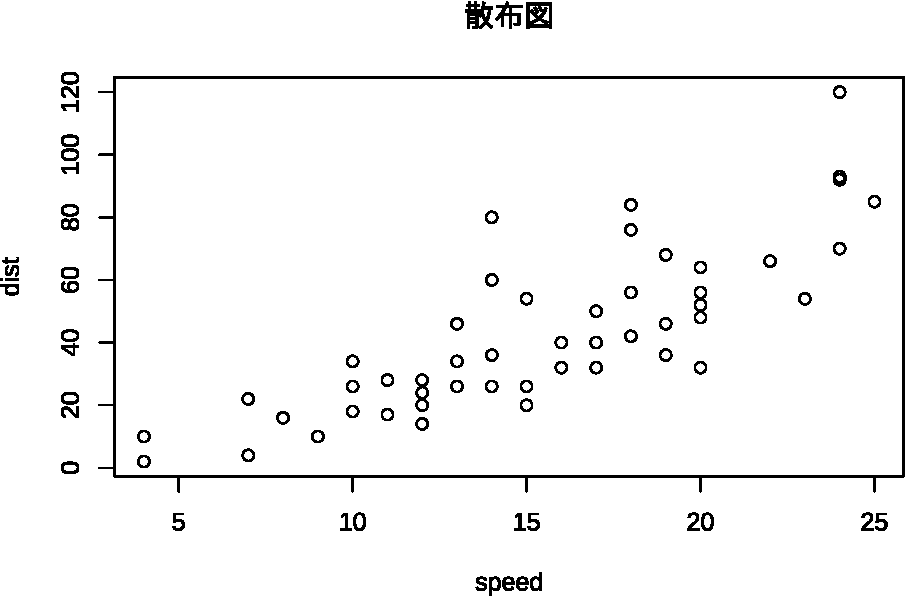
\includegraphics{26-visualize_files/figure-latex/unnamed-chunk-3-1.pdf}

さまざまな描画が可能ですが、一番、一般的な、散布図、\texttt{plot} に対応するものです。\texttt{ggplot} の中の、\texttt{aes} (aesthetic)の部分に、x 軸、y 軸に対応する変数(列名)を書きます。

\texttt{\textless{}DATA\textgreater{}\ \textbar{}\textgreater{}\ ggplot(aes(\textless{}変数\ x\ の列名\textgreater{},\ \textless{}変数\ y\ の列名\textgreater{}))\ +\ geom\_point()}

もっと明示的に

\texttt{\textless{}DATA\textgreater{}\ \textbar{}\textgreater{}\ ggplot(aes(x\ =\ \textless{}変数\ x\ の列名\textgreater{},\ y\ =\ \textless{}変数\ y\ の列名\textgreater{}))\ +\ geom\_point()}

さらには

\texttt{\textless{}DATA\textgreater{}\ \textbar{}\textgreater{}\ ggplot(mapping\ =\ aes(x\ =\ \textless{}変数\ x\ の列名\textgreater{},\ y\ =\ \textless{}変数\ y\ の列名\textgreater{}))\ +\ geom\_point()}

パイプを使わず

\texttt{ggplot(\textless{}DATA\textgreater{},\ aes(x\ =\ \textless{}変数\ x\ の列名\textgreater{},\ y\ =\ \textless{}変数\ y\ の列名\textgreater{}))\ +\ geom\_point()}

や、さらに、詳しく

\texttt{ggplot(data\ =\ \textless{}DATA\textgreater{},\ mapping\ =\ aes(x\ =\ \textless{}変数\ x\ の列名\textgreater{},\ y\ =\ \textless{}変数\ y\ の列名\textgreater{}))\ +\ geom\_point()}

も可能です。

種類(Species)ごとに色を変える場合には、\texttt{color\ =\ Species} とします。

\begin{Shaded}
\begin{Highlighting}[]
\NormalTok{df\_iris }\SpecialCharTok{|\textgreater{}} \FunctionTok{ggplot}\NormalTok{(}\FunctionTok{aes}\NormalTok{(Sepal.Width, Sepal.Length, }\AttributeTok{color =}\NormalTok{ Species)) }\SpecialCharTok{+}
  \FunctionTok{geom\_point}\NormalTok{()}
\end{Highlighting}
\end{Shaded}

\includegraphics{26-visualize_files/figure-latex/unnamed-chunk-4-1.pdf}

さらに、点の大きさを、Petal.Width によって変える場合には次のように、\texttt{size\ =\ Petal.Width} を加えます。

\begin{Shaded}
\begin{Highlighting}[]
\NormalTok{df\_iris }\SpecialCharTok{|\textgreater{}} 
  \FunctionTok{ggplot}\NormalTok{(}\FunctionTok{aes}\NormalTok{(Sepal.Width, Sepal.Length, }\AttributeTok{color =}\NormalTok{ Species, }
             \AttributeTok{size =}\NormalTok{ Petal.Width)) }\SpecialCharTok{+}
  \FunctionTok{geom\_point}\NormalTok{()}
\end{Highlighting}
\end{Shaded}

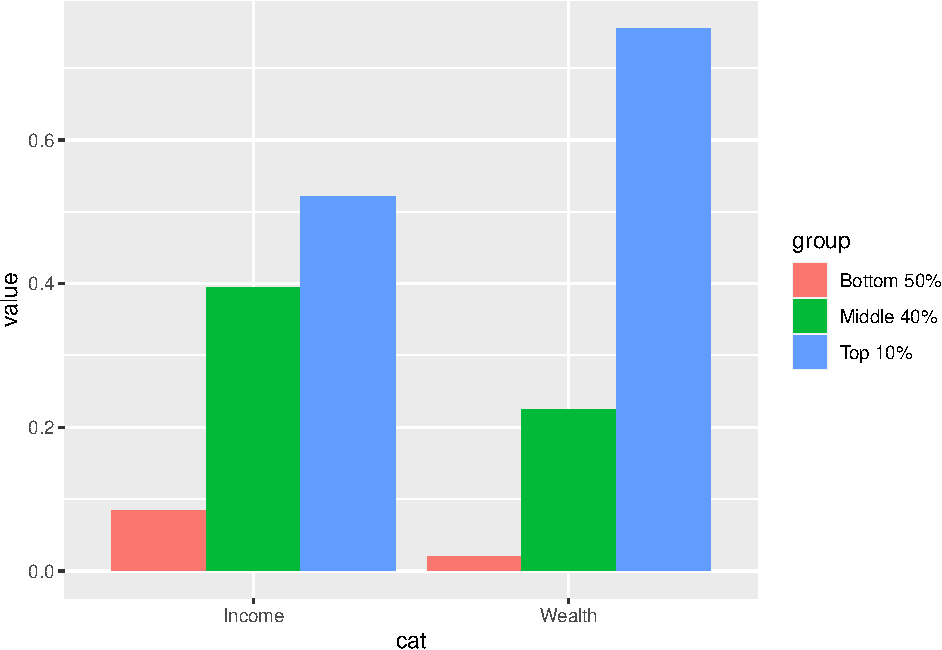
\includegraphics{26-visualize_files/figure-latex/unnamed-chunk-5-1.pdf}

ここでは、散布図でしたから、\texttt{geom\_point()} を使いましたが、これを他のものに変えていくと、さまざまなグラフが描けるようになっています。

\hypertarget{ux6563ux5e03ux56f3scatter-plot}{%
\section{散布図(Scatter Plot)}\label{ux6563ux5e03ux56f3scatter-plot}}

散布図は、データの二つの変数(列) を x と y に対応させる、最も基本的なグラフです。最初に試すべきグラフだともいうことができます。\texttt{mapping\ =} は省略することができます。

\begin{verbatim}
ggplot(data = <data>, aes(x = <column name for x>, y = <column name for y>)) +
  geom_point()
\end{verbatim}

\begin{verbatim}
ggplot(data = df_iris, aes(x = Sepal.Length, y = Sepal.Width)) +
  geom_point()
\end{verbatim}

変形(Transform)のときにつかった、\texttt{iris} データを使います。

\begin{Shaded}
\begin{Highlighting}[]
\FunctionTok{ggplot}\NormalTok{(}\AttributeTok{data =}\NormalTok{ df\_iris, }\FunctionTok{aes}\NormalTok{(}\AttributeTok{x =}\NormalTok{ Sepal.Length, }\AttributeTok{y =}\NormalTok{ Sepal.Width)) }\SpecialCharTok{+}
  \FunctionTok{geom\_point}\NormalTok{()}
\end{Highlighting}
\end{Shaded}

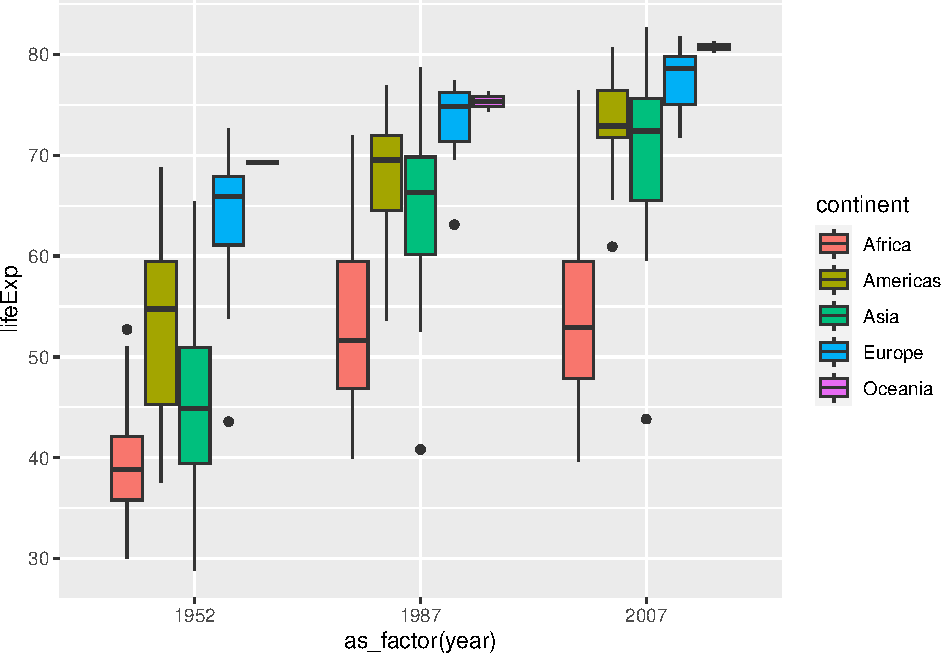
\includegraphics{26-visualize_files/figure-latex/unnamed-chunk-6-1.pdf}

\hypertarget{ux30e9ux30d9ux30eb-labels}{%
\subsection{\texorpdfstring{ラベル \href{https://ggplot2.tidyverse.org/reference/labs.html}{Labels}}{ラベル Labels}}\label{ux30e9ux30d9ux30eb-labels}}

グラフの表題や、x 軸、y 軸のラベルをつけるには \texttt{labs()} を使います。

\begin{verbatim}
ggplot(data = <data>, aes(x = <column name for x>, y = <column name for y>)) +
  geom_point() +
  labs(title = "Title", x = "Label for x", y = "Label for y")
\end{verbatim}

\begin{Shaded}
\begin{Highlighting}[]
\FunctionTok{ggplot}\NormalTok{(}\AttributeTok{data =}\NormalTok{ df\_iris, }\FunctionTok{aes}\NormalTok{(}\AttributeTok{x =}\NormalTok{ Sepal.Length, }\AttributeTok{y =}\NormalTok{ Sepal.Width)) }\SpecialCharTok{+}
  \FunctionTok{geom\_point}\NormalTok{() }\SpecialCharTok{+} 
  \FunctionTok{labs}\NormalTok{(}\AttributeTok{title =} \StringTok{"Scatter Plot of Sepal Data of Iris"}\NormalTok{, }\AttributeTok{x =} \StringTok{"Sepal Length"}\NormalTok{, }\AttributeTok{y =} \StringTok{"Sepal Width"}\NormalTok{)}
\end{Highlighting}
\end{Shaded}

\includegraphics{26-visualize_files/figure-latex/unnamed-chunk-7-1.pdf}

\begin{Shaded}
\begin{Highlighting}[]
\FunctionTok{ggplot}\NormalTok{(}\AttributeTok{data =}\NormalTok{ df\_iris, }\FunctionTok{aes}\NormalTok{(}\AttributeTok{x =}\NormalTok{ Sepal.Length, }\AttributeTok{y =}\NormalTok{ Sepal.Width)) }\SpecialCharTok{+}
  \FunctionTok{geom\_point}\NormalTok{() }\SpecialCharTok{+} 
  \FunctionTok{labs}\NormalTok{(}\AttributeTok{title =} \StringTok{"菖蒲の萼の長さと幅についての散布図"}\NormalTok{, }\AttributeTok{x =} \StringTok{"萼の長さ"}\NormalTok{, }\AttributeTok{y =} \StringTok{"萼の幅"}\NormalTok{)}
\end{Highlighting}
\end{Shaded}

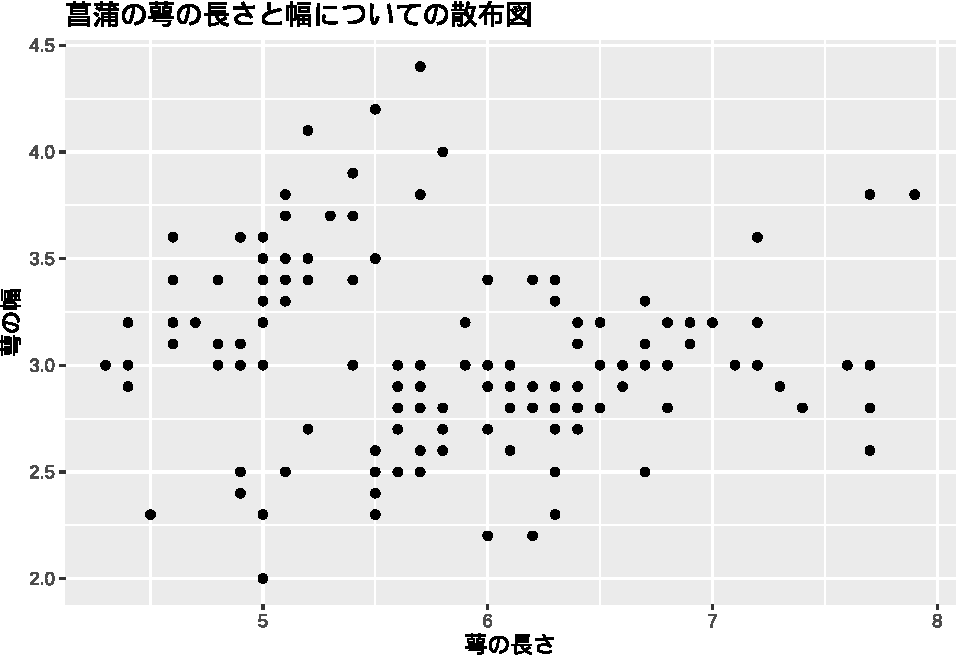
\includegraphics{26-visualize_files/figure-latex/unnamed-chunk-8-1.pdf}

このように、日本語をタイトルや、ラベルに使うことも可能ですが、以後は、データに日本語が含まれていない場合には、そのまま表示します。

\hypertarget{ux8272ux4ed8ux304d-colors}{%
\subsection{\texorpdfstring{色付き \href{https://ggplot2.tidyverse.org/reference/aes_colour_fill_alpha.html}{Colors}}{色付き Colors}}\label{ux8272ux4ed8ux304d-colors}}

菖蒲(iris)のデータは、Species 列に、三種類の菖蒲の名前が含まれていました。それぞれに、違う色で表示してみましょう。それには、x 軸、y 軸に対応する変数を指定したように、\texttt{color\ =\ Species} と指定します。

\begin{Shaded}
\begin{Highlighting}[]
\FunctionTok{ggplot}\NormalTok{(}\AttributeTok{data =}\NormalTok{ df\_iris, }\FunctionTok{aes}\NormalTok{(}\AttributeTok{x =}\NormalTok{ Sepal.Length, }\AttributeTok{y =}\NormalTok{ Sepal.Width, }\AttributeTok{color =}\NormalTok{ Species)) }\SpecialCharTok{+}
  \FunctionTok{geom\_point}\NormalTok{()}
\end{Highlighting}
\end{Shaded}

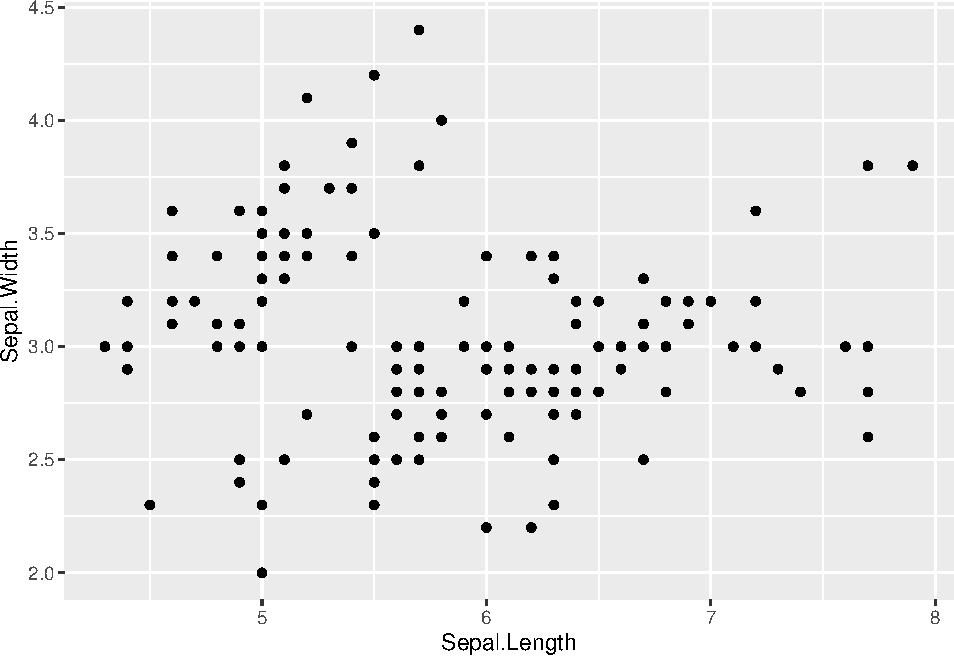
\includegraphics{26-visualize_files/figure-latex/unnamed-chunk-9-1.pdf}

\hypertarget{ux5f62ux72b6-shapes}{%
\subsection{\texorpdfstring{形状 \href{https://ggplot2.tidyverse.org/articles/ggplot2-specs.html}{Shapes}}{形状 Shapes}}\label{ux5f62ux72b6-shapes}}

色ではなく、形で Species を区別することも可能です。

\begin{Shaded}
\begin{Highlighting}[]
\FunctionTok{ggplot}\NormalTok{(}\AttributeTok{data =}\NormalTok{ df\_iris, }\FunctionTok{aes}\NormalTok{(}\AttributeTok{x =}\NormalTok{ Sepal.Length, }\AttributeTok{y =}\NormalTok{ Sepal.Width, }\AttributeTok{shape =}\NormalTok{ Species)) }\SpecialCharTok{+}
  \FunctionTok{geom\_point}\NormalTok{()}
\end{Highlighting}
\end{Shaded}

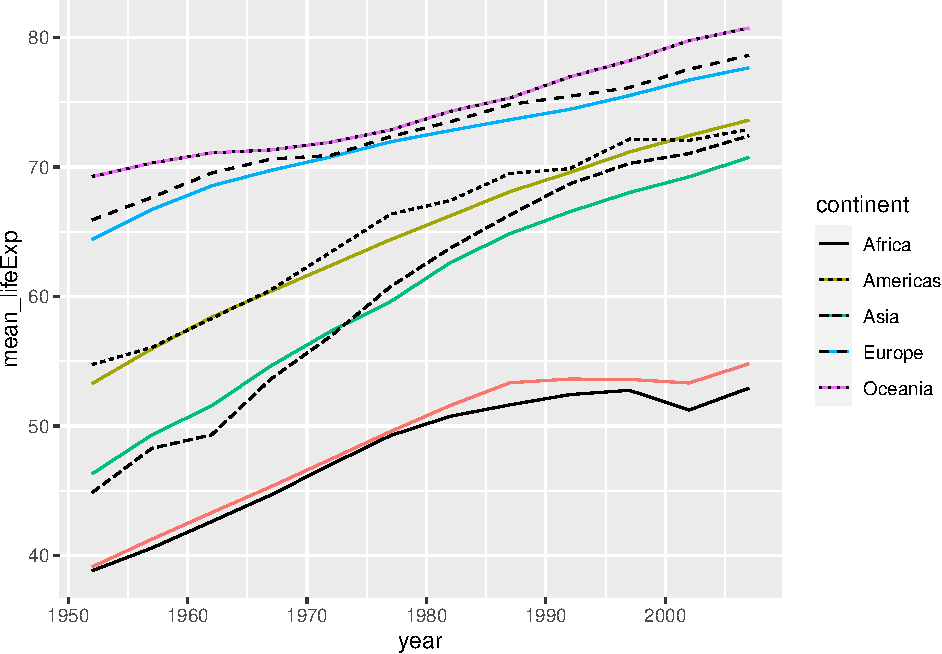
\includegraphics{26-visualize_files/figure-latex/unnamed-chunk-10-1.pdf}

色と、形、両方を同時に使うことも可能です。

\begin{Shaded}
\begin{Highlighting}[]
\FunctionTok{ggplot}\NormalTok{(}\AttributeTok{data =}\NormalTok{ df\_iris, }\FunctionTok{aes}\NormalTok{(}\AttributeTok{x =}\NormalTok{ Sepal.Length, }\AttributeTok{y =}\NormalTok{ Sepal.Width, }\AttributeTok{color =}\NormalTok{ Species, }\AttributeTok{shape =}\NormalTok{ Species)) }\SpecialCharTok{+}
  \FunctionTok{geom\_point}\NormalTok{()}
\end{Highlighting}
\end{Shaded}

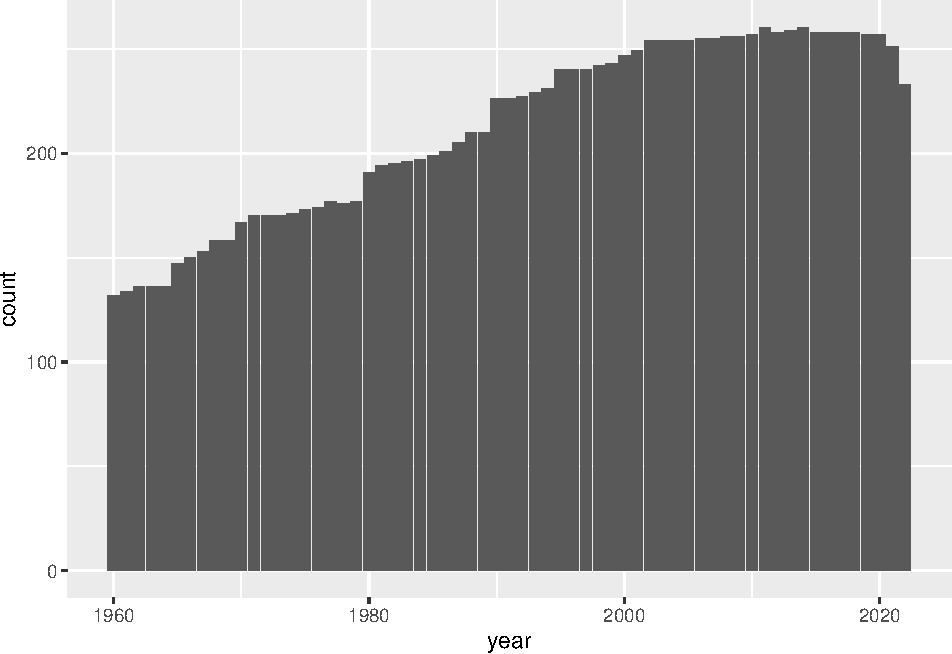
\includegraphics{26-visualize_files/figure-latex/unnamed-chunk-11-1.pdf}

\hypertarget{ux7bb1ux3072ux3052ux56f3-boxplot}{%
\section{\texorpdfstring{箱ひげ図 \href{https://ggplot2.tidyverse.org/reference/geom_boxplot.html}{Boxplot}}{箱ひげ図 Boxplot}}\label{ux7bb1ux3072ux3052ux56f3-boxplot}}

The boxplot compactly displays the distribution of a continuous variable.

箱ひげ図は、連続な値をとる変数の分布を簡潔な表示でみることができるグラフです。箱や、線の長さ、外れ値の表示なども、正確に決まっていますので、次のビデオをみてください。英語ですが、わかりやすく、まとまっていると思います。

\url{https://vimeo.com/222358034}

Transcript ボタンから、スクリプトを表示することもできます。

例のように、それぞれのグループごとに箱ひげ図を表示することもできますが、その場合は、文字データや、離散的な数値データ(いくつかの飛び飛びの値をとる変数)を使います。x と y を入れ替えれば、横向きになります。

\begin{Shaded}
\begin{Highlighting}[]
\FunctionTok{ggplot}\NormalTok{(}\AttributeTok{data =}\NormalTok{ df\_iris, }\FunctionTok{aes}\NormalTok{(}\AttributeTok{x =}\NormalTok{ Species, }\AttributeTok{y =}\NormalTok{ Sepal.Length)) }\SpecialCharTok{+}
  \FunctionTok{geom\_boxplot}\NormalTok{()}
\end{Highlighting}
\end{Shaded}

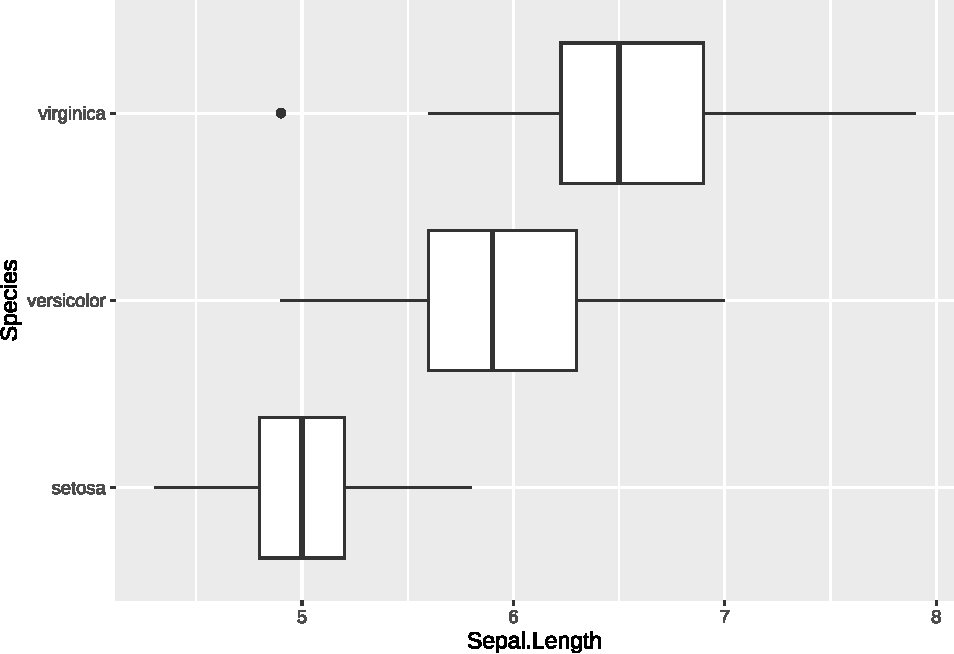
\includegraphics{26-visualize_files/figure-latex/unnamed-chunk-12-1.pdf}

\begin{Shaded}
\begin{Highlighting}[]
\FunctionTok{ggplot}\NormalTok{(}\AttributeTok{data =}\NormalTok{ df\_iris, }\FunctionTok{aes}\NormalTok{(}\AttributeTok{y =}\NormalTok{ Species, }\AttributeTok{x =}\NormalTok{ Sepal.Length)) }\SpecialCharTok{+}
  \FunctionTok{geom\_boxplot}\NormalTok{()}
\end{Highlighting}
\end{Shaded}

\includegraphics{26-visualize_files/figure-latex/unnamed-chunk-13-1.pdf}

各、種類(Species)ごとに、Sepal.Width(萼(がく)幅)が、どのように分布しているかを示しています。真ん中の太い線が、中央値(median)、箱が、第一四分位(Q1)から第三四分位(Q3)、線と点で表される外れ値も、どのような基準か定められています。(IQR = Q3-Q1, 線は、Q3+1.5\(\times\) IQR 以下に入っている実際の値までと、Q1-1.5 \(\times\) IQR 以上に入っている実際の値まで。それらに入っていないものが外れ値)。

color を指定すると、枠に色がつき、fill を指定すると、箱の中が塗り潰されます。

\begin{Shaded}
\begin{Highlighting}[]
\FunctionTok{ggplot}\NormalTok{(}\AttributeTok{data =}\NormalTok{ df\_iris, }\FunctionTok{aes}\NormalTok{(}\AttributeTok{x =}\NormalTok{ Species, }\AttributeTok{y =}\NormalTok{ Sepal.Length, }\AttributeTok{color =}\NormalTok{ Species)) }\SpecialCharTok{+}
  \FunctionTok{geom\_boxplot}\NormalTok{()}
\end{Highlighting}
\end{Shaded}

\includegraphics{26-visualize_files/figure-latex/unnamed-chunk-14-1.pdf}

\begin{Shaded}
\begin{Highlighting}[]
\FunctionTok{ggplot}\NormalTok{(}\AttributeTok{data =}\NormalTok{ df\_iris, }\FunctionTok{aes}\NormalTok{(}\AttributeTok{x =}\NormalTok{ Species, }\AttributeTok{y =}\NormalTok{ Sepal.Length, }\AttributeTok{fill =}\NormalTok{ Species)) }\SpecialCharTok{+}
  \FunctionTok{geom\_boxplot}\NormalTok{()}
\end{Highlighting}
\end{Shaded}

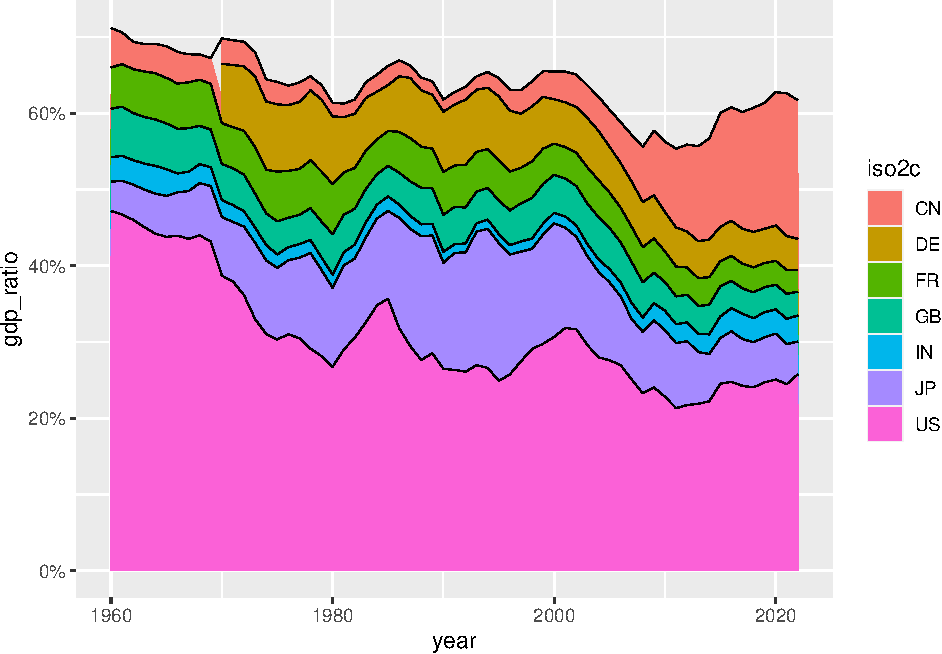
\includegraphics{26-visualize_files/figure-latex/unnamed-chunk-15-1.pdf}

\hypertarget{ux30d2ux30b9ux30c8ux30b0ux30e9ux30e0-histogram}{%
\subsection{\texorpdfstring{ヒストグラム \href{https://ggplot2.tidyverse.org/reference/geom_histogram.html}{Histogram}}{ヒストグラム Histogram}}\label{ux30d2ux30b9ux30c8ux30b0ux30e9ux30e0-histogram}}

Visualize the distribution of a single continuous variable by dividing the x axis into bins and counting the number of observations in each bin. Histograms (geom\_histogram()) display the counts with bars; frequency polygons (\texttt{geom\_freqpoly()}) display the counts with lines. Frequency polygons are more suitable when you want to compare the distribution across the levels of a categorical variable.

単一の連続変数の分布を可視化するために、x軸をビンに分割し、各ビン内の観測値の数を数えます。ヒストグラム(geom\_histogram())は、棒で数を表示します。一方、頻度多角形(geom\_freqpoly())は、数を線で表示します。頻度多角形は、カテゴリ変数のレベル間の分布を比較したい場合により適しています。

説明ビデオです。\url{https://vimeo.com/221607341}

\begin{Shaded}
\begin{Highlighting}[]
\FunctionTok{ggplot}\NormalTok{(}\AttributeTok{data =}\NormalTok{ df\_iris, }\FunctionTok{aes}\NormalTok{(}\AttributeTok{x =}\NormalTok{ Sepal.Length)) }\SpecialCharTok{+}
  \FunctionTok{geom\_histogram}\NormalTok{()}
\CommentTok{\#\textgreater{} \textasciigrave{}stat\_bin()\textasciigrave{} using \textasciigrave{}bins = 30\textasciigrave{}. Pick better value with}
\CommentTok{\#\textgreater{} \textasciigrave{}binwidth\textasciigrave{}.}
\end{Highlighting}
\end{Shaded}

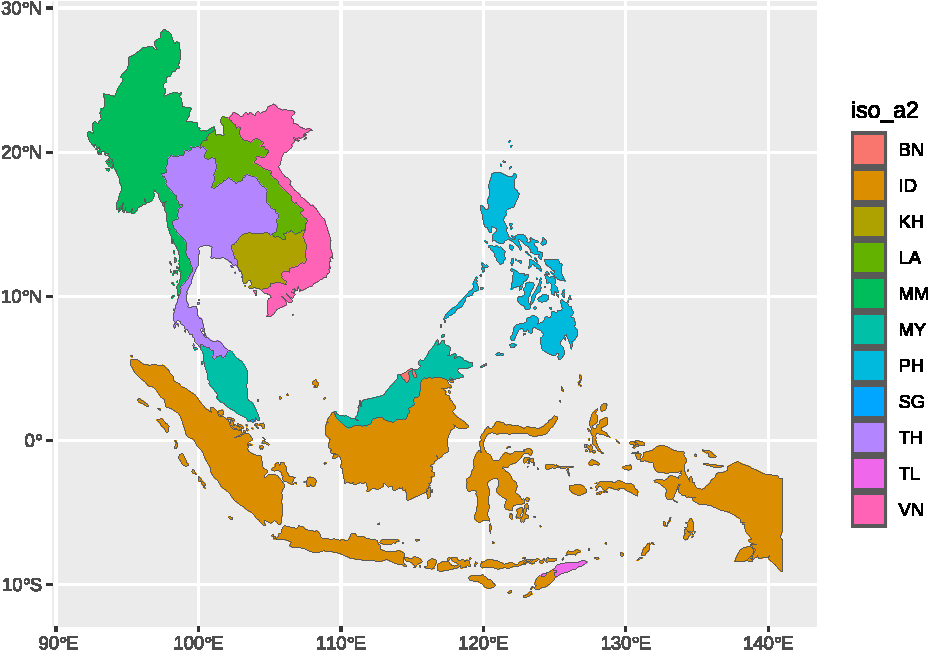
\includegraphics{26-visualize_files/figure-latex/unnamed-chunk-16-1.pdf}

枠(bins)を幾つに分けるか、または枠の幅を指定するようにとのメッセージが表示されます。

枠(bins)の数を変更するには \texttt{bins\ =} \texttt{\textless{}number\textgreater{}} を使います。幅を指定するときは、\texttt{binwidth\ =\ \textless{}number\textgreater{}} とします。

最初の例では、枠の個数を(初期設定では30になっているものを)10個とし、二つ目の例では、幅を1にしています。

\begin{Shaded}
\begin{Highlighting}[]
\FunctionTok{ggplot}\NormalTok{(}\AttributeTok{data =}\NormalTok{ df\_iris, }\FunctionTok{aes}\NormalTok{(}\AttributeTok{x =}\NormalTok{ Sepal.Length)) }\SpecialCharTok{+}
  \FunctionTok{geom\_histogram}\NormalTok{(}\AttributeTok{bins =} \DecValTok{10}\NormalTok{)}
\end{Highlighting}
\end{Shaded}

\includegraphics{26-visualize_files/figure-latex/unnamed-chunk-17-1.pdf}

\begin{Shaded}
\begin{Highlighting}[]
\FunctionTok{ggplot}\NormalTok{(}\AttributeTok{data =}\NormalTok{ df\_iris, }\FunctionTok{aes}\NormalTok{(}\AttributeTok{x =}\NormalTok{ Sepal.Length)) }\SpecialCharTok{+}
  \FunctionTok{geom\_histogram}\NormalTok{(}\AttributeTok{binwidth =} \DecValTok{1}\NormalTok{)}
\end{Highlighting}
\end{Shaded}

\includegraphics{26-visualize_files/figure-latex/unnamed-chunk-18-1.pdf}

頻度多角形(geom\_freqpoly())を使うと以下のようになります。Species ごとに比べたり、色をつけたりもできます。

\begin{Shaded}
\begin{Highlighting}[]
\FunctionTok{ggplot}\NormalTok{(}\AttributeTok{data =}\NormalTok{ df\_iris, }\FunctionTok{aes}\NormalTok{(}\AttributeTok{x =}\NormalTok{ Sepal.Length)) }\SpecialCharTok{+}
  \FunctionTok{geom\_freqpoly}\NormalTok{()}
\CommentTok{\#\textgreater{} \textasciigrave{}stat\_bin()\textasciigrave{} using \textasciigrave{}bins = 30\textasciigrave{}. Pick better value with}
\CommentTok{\#\textgreater{} \textasciigrave{}binwidth\textasciigrave{}.}
\end{Highlighting}
\end{Shaded}

\includegraphics{26-visualize_files/figure-latex/unnamed-chunk-19-1.pdf}

\begin{Shaded}
\begin{Highlighting}[]
\FunctionTok{ggplot}\NormalTok{(}\AttributeTok{data =}\NormalTok{ df\_iris, }\FunctionTok{aes}\NormalTok{(}\AttributeTok{x =}\NormalTok{ Sepal.Length, }\AttributeTok{color =}\NormalTok{ Species)) }\SpecialCharTok{+}
  \FunctionTok{geom\_freqpoly}\NormalTok{(}\AttributeTok{bins =} \DecValTok{10}\NormalTok{)}
\end{Highlighting}
\end{Shaded}

\includegraphics{26-visualize_files/figure-latex/unnamed-chunk-20-1.pdf}

滑らかな曲線にするときは、density plot を使います。alpha は透明度で 0 から 1 の値で指定します。数が小さい方が薄くなります。color で線の色もあわせて設定することも可能です。いろいろと試してみてください。

\begin{Shaded}
\begin{Highlighting}[]
\FunctionTok{ggplot}\NormalTok{(}\AttributeTok{data =}\NormalTok{ df\_iris, }\FunctionTok{aes}\NormalTok{(}\AttributeTok{x =}\NormalTok{ Sepal.Length, }\AttributeTok{fill =}\NormalTok{ Species)) }\SpecialCharTok{+}
  \FunctionTok{geom\_density}\NormalTok{(}\AttributeTok{alpha =} \FloatTok{0.5}\NormalTok{)}
\end{Highlighting}
\end{Shaded}

\includegraphics{26-visualize_files/figure-latex/unnamed-chunk-21-1.pdf}

\hypertarget{ux7ddaux5f62ux30e2ux30c7ux30eb-data-modeling}{%
\subsection{線形モデル Data Modeling}\label{ux7ddaux5f62ux30e2ux30c7ux30eb-data-modeling}}

回帰直線を加えたり、他の近似曲線を加えることも可能です。グラフとしても直感的理解を助けますが、統計的な扱いについては、Modeling で説明します。

\begin{Shaded}
\begin{Highlighting}[]
\FunctionTok{ggplot}\NormalTok{(}\AttributeTok{data =}\NormalTok{ df\_iris, }\FunctionTok{aes}\NormalTok{(}\AttributeTok{x =}\NormalTok{ Sepal.Length, }\AttributeTok{y =}\NormalTok{ Sepal.Width)) }\SpecialCharTok{+}
  \FunctionTok{geom\_point}\NormalTok{() }\SpecialCharTok{+}
  \FunctionTok{geom\_smooth}\NormalTok{(}\AttributeTok{method =} \StringTok{"lm"}\NormalTok{, }\AttributeTok{se =} \ConstantTok{FALSE}\NormalTok{)}
\end{Highlighting}
\end{Shaded}

\includegraphics{26-visualize_files/figure-latex/unnamed-chunk-22-1.pdf}

\begin{Shaded}
\begin{Highlighting}[]
\FunctionTok{ggplot}\NormalTok{(}\AttributeTok{data =}\NormalTok{ df\_iris, }\FunctionTok{aes}\NormalTok{(}\AttributeTok{x =}\NormalTok{ Sepal.Length, }\AttributeTok{y =}\NormalTok{ Sepal.Width)) }\SpecialCharTok{+}
  \FunctionTok{geom\_point}\NormalTok{() }\SpecialCharTok{+}
  \FunctionTok{geom\_smooth}\NormalTok{()}
\end{Highlighting}
\end{Shaded}

\includegraphics{26-visualize_files/figure-latex/unnamed-chunk-23-1.pdf}

\hypertarget{ux4f8bux304bux3089ux5b66ux3076-ggplot2-i}{%
\section{\texorpdfstring{例から学ぶ ggplot2\texttt{,} I}{例から学ぶ ggplot2, I}}\label{ux4f8bux304bux3089ux5b66ux3076-ggplot2-i}}

\hypertarget{mpg-ux3092ux4f7fux3063ux3066}{%
\subsubsection{mpg を使って}\label{mpg-ux3092ux4f7fux3063ux3066}}

\texttt{ggplot2} に含まれている、\texttt{mpg}(Fuel economy data from 1999 to 2008 for 38 popular models of cars - 1999年から2008年の38の型式の車の年燃費)データを使って、簡単な、散布図と、箱ひげ図を描いてみます。\texttt{mpg} の変数などについては、Help で調べてください。

manufacturer は、メーカー名、model は、型式、disp は、排気量(単位:リットル)、year は年式、cyl は、気筒数、trans は、オートマかマニュアルか、drv は、f が前輪駆動、r は後輪駆動、4 は四輪駆動、cty は街中での燃費(1ガロンで何マイル走るか)、hwy は高速道路での燃費(1ガロンで何マイル走るか)、fl 燃料の種類、class タイプ

\begin{Shaded}
\begin{Highlighting}[]
\NormalTok{df\_mpg }\OtherTok{\textless{}{-}}\NormalTok{ ggplot2}\SpecialCharTok{::}\NormalTok{mpg}
\NormalTok{df\_mpg}
\CommentTok{\#\textgreater{} \# A tibble: 234 x 11}
\CommentTok{\#\textgreater{}    manufacturer model    displ  year   cyl trans drv     cty}
\CommentTok{\#\textgreater{}    \textless{}chr\textgreater{}        \textless{}chr\textgreater{}    \textless{}dbl\textgreater{} \textless{}int\textgreater{} \textless{}int\textgreater{} \textless{}chr\textgreater{} \textless{}chr\textgreater{} \textless{}int\textgreater{}}
\CommentTok{\#\textgreater{}  1 audi         a4         1.8  1999     4 auto\textasciitilde{} f        18}
\CommentTok{\#\textgreater{}  2 audi         a4         1.8  1999     4 manu\textasciitilde{} f        21}
\CommentTok{\#\textgreater{}  3 audi         a4         2    2008     4 manu\textasciitilde{} f        20}
\CommentTok{\#\textgreater{}  4 audi         a4         2    2008     4 auto\textasciitilde{} f        21}
\CommentTok{\#\textgreater{}  5 audi         a4         2.8  1999     6 auto\textasciitilde{} f        16}
\CommentTok{\#\textgreater{}  6 audi         a4         2.8  1999     6 manu\textasciitilde{} f        18}
\CommentTok{\#\textgreater{}  7 audi         a4         3.1  2008     6 auto\textasciitilde{} f        18}
\CommentTok{\#\textgreater{}  8 audi         a4 quat\textasciitilde{}   1.8  1999     4 manu\textasciitilde{} 4        18}
\CommentTok{\#\textgreater{}  9 audi         a4 quat\textasciitilde{}   1.8  1999     4 auto\textasciitilde{} 4        16}
\CommentTok{\#\textgreater{} 10 audi         a4 quat\textasciitilde{}   2    2008     4 manu\textasciitilde{} 4        20}
\CommentTok{\#\textgreater{} \# i 224 more rows}
\CommentTok{\#\textgreater{} \# i 3 more variables: hwy \textless{}int\textgreater{}, fl \textless{}chr\textgreater{}, class \textless{}chr\textgreater{}}
\end{Highlighting}
\end{Shaded}

\begin{Shaded}
\begin{Highlighting}[]
\FunctionTok{glimpse}\NormalTok{(df\_mpg)}
\CommentTok{\#\textgreater{} Rows: 234}
\CommentTok{\#\textgreater{} Columns: 11}
\CommentTok{\#\textgreater{} $ manufacturer \textless{}chr\textgreater{} "audi", "audi", "audi", "audi", "audi\textasciitilde{}}
\CommentTok{\#\textgreater{} $ model        \textless{}chr\textgreater{} "a4", "a4", "a4", "a4", "a4", "a4", "\textasciitilde{}}
\CommentTok{\#\textgreater{} $ displ        \textless{}dbl\textgreater{} 1.8, 1.8, 2.0, 2.0, 2.8, 2.8, 3.1, 1.\textasciitilde{}}
\CommentTok{\#\textgreater{} $ year         \textless{}int\textgreater{} 1999, 1999, 2008, 2008, 1999, 1999, 2\textasciitilde{}}
\CommentTok{\#\textgreater{} $ cyl          \textless{}int\textgreater{} 4, 4, 4, 4, 6, 6, 6, 4, 4, 4, 4, 6, 6\textasciitilde{}}
\CommentTok{\#\textgreater{} $ trans        \textless{}chr\textgreater{} "auto(l5)", "manual(m5)", "manual(m6)\textasciitilde{}}
\CommentTok{\#\textgreater{} $ drv          \textless{}chr\textgreater{} "f", "f", "f", "f", "f", "f", "f", "4\textasciitilde{}}
\CommentTok{\#\textgreater{} $ cty          \textless{}int\textgreater{} 18, 21, 20, 21, 16, 18, 18, 18, 16, 2\textasciitilde{}}
\CommentTok{\#\textgreater{} $ hwy          \textless{}int\textgreater{} 29, 29, 31, 30, 26, 26, 27, 26, 25, 2\textasciitilde{}}
\CommentTok{\#\textgreater{} $ fl           \textless{}chr\textgreater{} "p", "p", "p", "p", "p", "p", "p", "p\textasciitilde{}}
\CommentTok{\#\textgreater{} $ class        \textless{}chr\textgreater{} "compact", "compact", "compact", "com\textasciitilde{}}
\end{Highlighting}
\end{Shaded}

\begin{Shaded}
\begin{Highlighting}[]
\FunctionTok{ggplot}\NormalTok{(}\AttributeTok{data =}\NormalTok{ df\_mpg) }\SpecialCharTok{+} \FunctionTok{geom\_point}\NormalTok{(}\AttributeTok{mapping =} \FunctionTok{aes}\NormalTok{(}\AttributeTok{x =}\NormalTok{ displ, }\AttributeTok{y =}\NormalTok{ hwy))}
\end{Highlighting}
\end{Shaded}

\includegraphics{26-visualize_files/figure-latex/unnamed-chunk-26-1.pdf}

\begin{Shaded}
\begin{Highlighting}[]
\FunctionTok{ggplot}\NormalTok{(}\AttributeTok{data =}\NormalTok{ df\_mpg) }\SpecialCharTok{+} \FunctionTok{geom\_boxplot}\NormalTok{(}\AttributeTok{mapping =} \FunctionTok{aes}\NormalTok{(}\AttributeTok{x =}\NormalTok{ class, }\AttributeTok{y =}\NormalTok{ hwy))}
\end{Highlighting}
\end{Shaded}

\includegraphics{26-visualize_files/figure-latex/unnamed-chunk-27-1.pdf}

\begin{enumerate}
\def\labelenumi{\arabic{enumi}.}
\item
  \texttt{data\ =\ df\_mpg} でデータを指定します。
\item
  どのようなグラフにするか、幾何関数(Geometric Function)を指定します。散布図では、\texttt{geom\_pont()} 、箱ひげ図では、\texttt{geom\_boxplot()} などです。
\item
  x 軸、y 軸などに対応する変数の写像(mapping)を指定します。

  \begin{itemize}
  \item
    散布図では、\texttt{dspl} (displacemnt エンジンの排気量(単位 リットル))を x 軸に、\texttt{hwy} 高速道路で1ガロンで走れる距離(単位 マイル)を y 軸に割り当てています。
  \item
    箱ひげ図では、\texttt{class} 車の型式を、x 軸に、\texttt{hwy} 高速道路で1ガロンで走れる距離(単位 マイル)を y 軸に割り当てています。
  \end{itemize}
\end{enumerate}

記号的に書くと、下のようになっています。

\texttt{ggplot(data\ =\ \textless{}DATA\textgreater{})\ +\ \textless{}GEOM\_FUNCTION\textgreater{}(mapping\ =\ aes(\textless{}MAPPINGS\textgreater{}))}

\hypertarget{ux4f8bux304bux3089ux5b66ux3076-ggplot2-ii}{%
\section{\texorpdfstring{例から学ぶ ggplot2\texttt{,} II}{例から学ぶ ggplot2, II}}\label{ux4f8bux304bux3089ux5b66ux3076-ggplot2-ii}}

\hypertarget{df_wdi-df_wdi_extra-1}{%
\subsection{df\_wdi, df\_wdi\_extra}\label{df_wdi-df_wdi_extra-1}}

前の章の \texttt{Tidyverse} で読み込み、概観した、世界開発指標(World Development Indicators)のデータを使います。\href{https://icu-hsuzuki.github.io/ds4aj/tidyverse.html\#wdi-のデータ}{参照:WDI のデータ}

\begin{Shaded}
\begin{Highlighting}[]
\FunctionTok{library}\NormalTok{(tidyverse)}
\FunctionTok{library}\NormalTok{(WDI)}
\end{Highlighting}
\end{Shaded}

WDI の使い方は、世界銀行の部分で紹介しますが、はじめてのデータサイエンスの例でも紹介したように、データコードを利用して、データを読み込みます。ここでは、出生時の平均寿命と、一人当たりの GDP と、総人口のデータを使います。

\begin{itemize}
\tightlist
\item
  SP.DYN.LE00.IN: Life expectancy at birth, total (years) 出生時の平均寿命
\item
  SP.POP.TOTL: Population, total 総人口
\item
  NY.GDP.PCAP.KD: GDP per capita (constant 2015 US\$) 一人当たりの GDP
\end{itemize}

次のコードで読み込みます。

\begin{Shaded}
\begin{Highlighting}[]
\NormalTok{df\_wdi }\OtherTok{\textless{}{-}} \FunctionTok{WDI}\NormalTok{(}
  \AttributeTok{country =} \StringTok{"all"}\NormalTok{, }
  \AttributeTok{indicator =} \FunctionTok{c}\NormalTok{(}\AttributeTok{lifeExp =} \StringTok{"SP.DYN.LE00.IN"}\NormalTok{, }\AttributeTok{pop =} \StringTok{"SP.POP.TOTL"}\NormalTok{, }\AttributeTok{gdpPercap =} \StringTok{"NY.GDP.PCAP.KD"}\NormalTok{)}
\NormalTok{)}
\end{Highlighting}
\end{Shaded}

\begin{verbatim}
#> Rows: 16758 Columns: 7
#> -- Column specification ------------------------------------
#> Delimiter: ","
#> chr (3): country, iso2c, iso3c
#> dbl (4): year, lifeExp, pop, gdpPercap
#> 
#> i Use `spec()` to retrieve the full column specification for this data.
#> i Specify the column types or set `show_col_types = FALSE` to quiet this message.
\end{verbatim}

\begin{Shaded}
\begin{Highlighting}[]
\NormalTok{df\_wdi\_extra }\OtherTok{\textless{}{-}} \FunctionTok{WDI}\NormalTok{(}
  \AttributeTok{country =} \StringTok{"all"}\NormalTok{, }
  \AttributeTok{indicator =} \FunctionTok{c}\NormalTok{(}\AttributeTok{lifeExp =} \StringTok{"SP.DYN.LE00.IN"}\NormalTok{, }\AttributeTok{pop =} \StringTok{"SP.POP.TOTL"}\NormalTok{, }\AttributeTok{gdpPercap =} \StringTok{"NY.GDP.PCAP.KD"}\NormalTok{), }
  \AttributeTok{extra =} \ConstantTok{TRUE}
\NormalTok{)}
\end{Highlighting}
\end{Shaded}

すこし、追加情報を付加したものも取得しておきます。

\begin{verbatim}
#> Rows: 16758 Columns: 15
#> -- Column specification ------------------------------------
#> Delimiter: ","
#> chr  (7): country, iso2c, iso3c, region, capital, income...
#> dbl  (6): year, lifeExp, pop, gdpPercap, longitude, lati...
#> lgl  (1): status
#> date (1): lastupdated
#> 
#> i Use `spec()` to retrieve the full column specification for this data.
#> i Specify the column types or set `show_col_types = FALSE` to quiet this message.
\end{verbatim}

\begin{Shaded}
\begin{Highlighting}[]
\NormalTok{df\_wdi}
\CommentTok{\#\textgreater{} \# A tibble: 16,758 x 7}
\CommentTok{\#\textgreater{}    country     iso2c iso3c  year lifeExp      pop gdpPercap}
\CommentTok{\#\textgreater{}    \textless{}chr\textgreater{}       \textless{}chr\textgreater{} \textless{}chr\textgreater{} \textless{}dbl\textgreater{}   \textless{}dbl\textgreater{}    \textless{}dbl\textgreater{}     \textless{}dbl\textgreater{}}
\CommentTok{\#\textgreater{}  1 Afghanistan AF    AFG    1960    32.5  8622466        NA}
\CommentTok{\#\textgreater{}  2 Afghanistan AF    AFG    1961    33.1  8790140        NA}
\CommentTok{\#\textgreater{}  3 Afghanistan AF    AFG    1962    33.5  8969047        NA}
\CommentTok{\#\textgreater{}  4 Afghanistan AF    AFG    1963    34.0  9157465        NA}
\CommentTok{\#\textgreater{}  5 Afghanistan AF    AFG    1964    34.5  9355514        NA}
\CommentTok{\#\textgreater{}  6 Afghanistan AF    AFG    1965    35.0  9565147        NA}
\CommentTok{\#\textgreater{}  7 Afghanistan AF    AFG    1966    35.5  9783147        NA}
\CommentTok{\#\textgreater{}  8 Afghanistan AF    AFG    1967    35.9 10010030        NA}
\CommentTok{\#\textgreater{}  9 Afghanistan AF    AFG    1968    36.4 10247780        NA}
\CommentTok{\#\textgreater{} 10 Afghanistan AF    AFG    1969    36.9 10494489        NA}
\CommentTok{\#\textgreater{} \# i 16,748 more rows}
\end{Highlighting}
\end{Shaded}

\hypertarget{section-1}{%
\subsection{}\label{section-1}}

\hypertarget{ux6298ux7ddaux30b0ux30e9ux30d5line-graph}{%
\subsection{\texorpdfstring{\textbf{折線グラフ(line graph)}}{折線グラフ(line graph)}}\label{ux6298ux7ddaux30b0ux30e9ux30d5line-graph}}

WDI は時系列データですから、折れ線グラフも使います。後ほど紹介しますが、

\texttt{\textless{}DATA\textgreater{}\ \textbar{}\textgreater{}\ ggplot(aes(year,\ lifeExp))\ +\ geom\_line()}

と言った感じです。

まずは、失敗例から。次のコードでグラフが描けるでしょうか。

\begin{Shaded}
\begin{Highlighting}[]
\NormalTok{df\_wdi }\SpecialCharTok{|\textgreater{}} \FunctionTok{ggplot}\NormalTok{(}\FunctionTok{aes}\NormalTok{(year, lifeExp)) }\SpecialCharTok{+} \FunctionTok{geom\_line}\NormalTok{()}
\CommentTok{\#\textgreater{} Warning: Removed 266 rows containing missing values}
\CommentTok{\#\textgreater{} (\textasciigrave{}geom\_line()\textasciigrave{}).}
\end{Highlighting}
\end{Shaded}

\includegraphics{26-visualize_files/figure-latex/unnamed-chunk-36-1.pdf}

何が起こっているかわかりますか。これは、鋸の刃グラフ(saw-tooth chart)と言われる標準的な失敗例です。

\begin{Shaded}
\begin{Highlighting}[]
\FunctionTok{ggplot}\NormalTok{(df\_wdi, }\FunctionTok{aes}\NormalTok{(}\AttributeTok{x =}\NormalTok{ year, }\AttributeTok{y =}\NormalTok{ lifeExp)) }\SpecialCharTok{+} \FunctionTok{geom\_boxplot}\NormalTok{()}
\CommentTok{\#\textgreater{} Warning: Continuous x aesthetic}
\CommentTok{\#\textgreater{} i did you forget \textasciigrave{}aes(group = ...)\textasciigrave{}?}
\CommentTok{\#\textgreater{} Warning: Removed 892 rows containing non{-}finite values}
\CommentTok{\#\textgreater{} (\textasciigrave{}stat\_boxplot()\textasciigrave{}).}
\end{Highlighting}
\end{Shaded}

\includegraphics{26-visualize_files/figure-latex/unnamed-chunk-37-1.pdf}

これも期待した箱ひげ図にはなっていません。年は、カテゴリーではなく、数値データですね。

\begin{Shaded}
\begin{Highlighting}[]
\FunctionTok{typeof}\NormalTok{(}\FunctionTok{pull}\NormalTok{(df\_wdi, year)) }\CommentTok{\# same as typeof(df$year)}
\CommentTok{\#\textgreater{} [1] "double"}
\end{Highlighting}
\end{Shaded}

次のようにすると少しマシになります。

\begin{Shaded}
\begin{Highlighting}[]
\FunctionTok{ggplot}\NormalTok{(df\_wdi, }\FunctionTok{aes}\NormalTok{(}\AttributeTok{y =}\NormalTok{ lifeExp, }\AttributeTok{group =}\NormalTok{ year)) }\SpecialCharTok{+} \FunctionTok{geom\_boxplot}\NormalTok{()}
\CommentTok{\#\textgreater{} Warning: Removed 892 rows containing non{-}finite values}
\CommentTok{\#\textgreater{} (\textasciigrave{}stat\_boxplot()\textasciigrave{}).}
\end{Highlighting}
\end{Shaded}

\includegraphics{26-visualize_files/figure-latex/unnamed-chunk-39-1.pdf}

\hypertarget{box-plot}{%
\paragraph{Box Plot}\label{box-plot}}

\begin{Shaded}
\begin{Highlighting}[]
\FunctionTok{ggplot}\NormalTok{(df\_wdi, }\FunctionTok{aes}\NormalTok{(}\AttributeTok{x =} \FunctionTok{as\_factor}\NormalTok{(year), }\AttributeTok{y =}\NormalTok{ lifeExp)) }\SpecialCharTok{+} \FunctionTok{geom\_boxplot}\NormalTok{()}
\CommentTok{\#\textgreater{} Warning: Removed 892 rows containing non{-}finite values}
\CommentTok{\#\textgreater{} (\textasciigrave{}stat\_boxplot()\textasciigrave{}).}
\end{Highlighting}
\end{Shaded}

\includegraphics{26-visualize_files/figure-latex/unnamed-chunk-40-1.pdf}

とはいえ、数が多すぎますね。色もつけてみましょう。塗りつぶしは、fill 枠の線に色をつけるのは、color ですから、ここでは、fill を使います。

\begin{Shaded}
\begin{Highlighting}[]
\NormalTok{df\_wdi\_extra }\SpecialCharTok{|\textgreater{}} \FunctionTok{filter}\NormalTok{(income }\SpecialCharTok{!=} \StringTok{"Aggregates"}\NormalTok{) }\SpecialCharTok{|\textgreater{}} 
  \FunctionTok{filter}\NormalTok{(year }\SpecialCharTok{\%in\%} \FunctionTok{c}\NormalTok{(}\DecValTok{1960}\NormalTok{, }\DecValTok{1980}\NormalTok{, }\DecValTok{2000}\NormalTok{, }\DecValTok{2020}\NormalTok{)) }\SpecialCharTok{|\textgreater{}}
  \FunctionTok{ggplot}\NormalTok{(}\FunctionTok{aes}\NormalTok{(}\AttributeTok{x=}\FunctionTok{as\_factor}\NormalTok{(year), }\AttributeTok{y =}\NormalTok{ lifeExp, }\AttributeTok{fill =}\NormalTok{ income)) }\SpecialCharTok{+}
  \FunctionTok{geom\_boxplot}\NormalTok{()}
\CommentTok{\#\textgreater{} Warning: Removed 37 rows containing non{-}finite values}
\CommentTok{\#\textgreater{} (\textasciigrave{}stat\_boxplot()\textasciigrave{}).}
\end{Highlighting}
\end{Shaded}

\includegraphics{26-visualize_files/figure-latex/unnamed-chunk-41-1.pdf}

折線グラフの例としては次のようなものがあります。

\begin{Shaded}
\begin{Highlighting}[]
\NormalTok{df\_lifeExp }\OtherTok{\textless{}{-}}\NormalTok{ df\_wdi\_extra }\SpecialCharTok{|\textgreater{}} \FunctionTok{filter}\NormalTok{(region }\SpecialCharTok{!=} \StringTok{"Aggregates"}\NormalTok{) }\SpecialCharTok{|\textgreater{}}  
  \FunctionTok{group\_by}\NormalTok{(region, year) }\SpecialCharTok{|\textgreater{}}
  \FunctionTok{summarize}\NormalTok{(}\AttributeTok{mean\_lifeExp =} \FunctionTok{mean}\NormalTok{(lifeExp), }\AttributeTok{median\_lifeExp =} \FunctionTok{median}\NormalTok{(lifeExp), }\AttributeTok{max\_lifeExp =} \FunctionTok{max}\NormalTok{(lifeExp), }\AttributeTok{min\_lifeExp =} \FunctionTok{min}\NormalTok{(lifeExp), }\AttributeTok{.groups =} \StringTok{"keep"}\NormalTok{)}
\end{Highlighting}
\end{Shaded}

\begin{Shaded}
\begin{Highlighting}[]
\NormalTok{df\_lifeExp }\SpecialCharTok{\%\textgreater{}\%} \FunctionTok{ggplot}\NormalTok{(}\FunctionTok{aes}\NormalTok{(}\AttributeTok{x =}\NormalTok{ year, }\AttributeTok{y =}\NormalTok{ mean\_lifeExp, }\AttributeTok{color =}\NormalTok{ region)) }\SpecialCharTok{+}
  \FunctionTok{geom\_line}\NormalTok{()}
\CommentTok{\#\textgreater{} Warning: Removed 243 rows containing missing values}
\CommentTok{\#\textgreater{} (\textasciigrave{}geom\_line()\textasciigrave{}).}
\end{Highlighting}
\end{Shaded}

\includegraphics{26-visualize_files/figure-latex/unnamed-chunk-43-1.pdf}

\begin{Shaded}
\begin{Highlighting}[]
\NormalTok{df\_lifeExp }\SpecialCharTok{\%\textgreater{}\%} \FunctionTok{ggplot}\NormalTok{(}\FunctionTok{aes}\NormalTok{(}\AttributeTok{x =}\NormalTok{ year, }\AttributeTok{y =}\NormalTok{ mean\_lifeExp, }\AttributeTok{color =}\NormalTok{ region, }\AttributeTok{linetype =}\NormalTok{ region)) }\SpecialCharTok{+}
  \FunctionTok{geom\_line}\NormalTok{()}
\CommentTok{\#\textgreater{} Warning: Removed 243 rows containing missing values}
\CommentTok{\#\textgreater{} (\textasciigrave{}geom\_line()\textasciigrave{}).}
\end{Highlighting}
\end{Shaded}

\includegraphics{26-visualize_files/figure-latex/unnamed-chunk-44-1.pdf}

\begin{Shaded}
\begin{Highlighting}[]
\NormalTok{df\_lifeExp }\SpecialCharTok{\%\textgreater{}\%} \FunctionTok{ggplot}\NormalTok{() }\SpecialCharTok{+}
  \FunctionTok{geom\_line}\NormalTok{(}\FunctionTok{aes}\NormalTok{(}\AttributeTok{x =}\NormalTok{ year, }\AttributeTok{y =}\NormalTok{ mean\_lifeExp, }\AttributeTok{color =}\NormalTok{ region)) }\SpecialCharTok{+} 
  \FunctionTok{geom\_line}\NormalTok{(}\FunctionTok{aes}\NormalTok{(}\AttributeTok{x =}\NormalTok{ year, }\AttributeTok{y =}\NormalTok{ median\_lifeExp, }\AttributeTok{linetype =}\NormalTok{ region))}
\CommentTok{\#\textgreater{} Warning: Removed 243 rows containing missing values (\textasciigrave{}geom\_line()\textasciigrave{}).}
\CommentTok{\#\textgreater{} Removed 243 rows containing missing values (\textasciigrave{}geom\_line()\textasciigrave{}).}
\end{Highlighting}
\end{Shaded}

\includegraphics{26-visualize_files/figure-latex/unnamed-chunk-45-1.pdf}

\hypertarget{wdi-1}{%
\subsubsection{WDI}\label{wdi-1}}

\begin{itemize}
\tightlist
\item
  SP.DYN.LE00.IN: Life expectancy at birth, total (years)
\item
  NY.GDP.PCAP.KD: GDP per capita (constant 2015 US\$)
\item
  SP.POP.TOTL: Population, total
\end{itemize}

\begin{Shaded}
\begin{Highlighting}[]
\NormalTok{df\_wdi }\OtherTok{\textless{}{-}} \FunctionTok{WDI}\NormalTok{(}
  \AttributeTok{country =} \StringTok{"all"}\NormalTok{, }
  \AttributeTok{indicator =} \FunctionTok{c}\NormalTok{(}\AttributeTok{lifeExp =} \StringTok{"SP.DYN.LE00.IN"}\NormalTok{, }\AttributeTok{pop =} \StringTok{"SP.POP.TOTL"}\NormalTok{, }\AttributeTok{gdpPercap =} \StringTok{"NY.GDP.PCAP.KD"}\NormalTok{)}
\NormalTok{)}
\end{Highlighting}
\end{Shaded}

\begin{verbatim}
#> Rows: 16758 Columns: 7
#> -- Column specification ------------------------------------
#> Delimiter: ","
#> chr (3): country, iso2c, iso3c
#> dbl (4): year, lifeExp, pop, gdpPercap
#> 
#> i Use `spec()` to retrieve the full column specification for this data.
#> i Specify the column types or set `show_col_types = FALSE` to quiet this message.
\end{verbatim}

\begin{Shaded}
\begin{Highlighting}[]
\NormalTok{df\_wdi }\SpecialCharTok{\%\textgreater{}\%} \FunctionTok{slice}\NormalTok{(}\DecValTok{1}\SpecialCharTok{:}\DecValTok{10}\NormalTok{)}
\CommentTok{\#\textgreater{} \# A tibble: 10 x 7}
\CommentTok{\#\textgreater{}    country     iso2c iso3c  year lifeExp      pop gdpPercap}
\CommentTok{\#\textgreater{}    \textless{}chr\textgreater{}       \textless{}chr\textgreater{} \textless{}chr\textgreater{} \textless{}dbl\textgreater{}   \textless{}dbl\textgreater{}    \textless{}dbl\textgreater{}     \textless{}dbl\textgreater{}}
\CommentTok{\#\textgreater{}  1 Afghanistan AF    AFG    1960    32.5  8622466        NA}
\CommentTok{\#\textgreater{}  2 Afghanistan AF    AFG    1961    33.1  8790140        NA}
\CommentTok{\#\textgreater{}  3 Afghanistan AF    AFG    1962    33.5  8969047        NA}
\CommentTok{\#\textgreater{}  4 Afghanistan AF    AFG    1963    34.0  9157465        NA}
\CommentTok{\#\textgreater{}  5 Afghanistan AF    AFG    1964    34.5  9355514        NA}
\CommentTok{\#\textgreater{}  6 Afghanistan AF    AFG    1965    35.0  9565147        NA}
\CommentTok{\#\textgreater{}  7 Afghanistan AF    AFG    1966    35.5  9783147        NA}
\CommentTok{\#\textgreater{}  8 Afghanistan AF    AFG    1967    35.9 10010030        NA}
\CommentTok{\#\textgreater{}  9 Afghanistan AF    AFG    1968    36.4 10247780        NA}
\CommentTok{\#\textgreater{} 10 Afghanistan AF    AFG    1969    36.9 10494489        NA}
\end{Highlighting}
\end{Shaded}

\begin{Shaded}
\begin{Highlighting}[]
\NormalTok{df\_wdi\_extra }\OtherTok{\textless{}{-}} \FunctionTok{WDI}\NormalTok{(}
  \AttributeTok{country =} \StringTok{"all"}\NormalTok{, }
  \AttributeTok{indicator =} \FunctionTok{c}\NormalTok{(}\AttributeTok{lifeExp =} \StringTok{"SP.DYN.LE00.IN"}\NormalTok{, }\AttributeTok{pop =} \StringTok{"SP.POP.TOTL"}\NormalTok{, }\AttributeTok{gdpPercap =} \StringTok{"NY.GDP.PCAP.KD"}\NormalTok{), }
  \AttributeTok{extra =} \ConstantTok{TRUE}
\NormalTok{)}
\end{Highlighting}
\end{Shaded}

\begin{verbatim}
#> Rows: 16758 Columns: 15
#> -- Column specification ------------------------------------
#> Delimiter: ","
#> chr  (7): country, iso2c, iso3c, region, capital, income...
#> dbl  (6): year, lifeExp, pop, gdpPercap, longitude, lati...
#> lgl  (1): status
#> date (1): lastupdated
#> 
#> i Use `spec()` to retrieve the full column specification for this data.
#> i Specify the column types or set `show_col_types = FALSE` to quiet this message.
\end{verbatim}

\begin{Shaded}
\begin{Highlighting}[]
\NormalTok{df\_wdi\_extra}
\CommentTok{\#\textgreater{} \# A tibble: 16,758 x 15}
\CommentTok{\#\textgreater{}    country     iso2c iso3c  year status lastupdated lifeExp}
\CommentTok{\#\textgreater{}    \textless{}chr\textgreater{}       \textless{}chr\textgreater{} \textless{}chr\textgreater{} \textless{}dbl\textgreater{} \textless{}lgl\textgreater{}  \textless{}date\textgreater{}        \textless{}dbl\textgreater{}}
\CommentTok{\#\textgreater{}  1 Afghanistan AF    AFG    2014 NA     2023{-}07{-}25     62.5}
\CommentTok{\#\textgreater{}  2 Afghanistan AF    AFG    2012 NA     2023{-}07{-}25     61.9}
\CommentTok{\#\textgreater{}  3 Afghanistan AF    AFG    2009 NA     2023{-}07{-}25     60.4}
\CommentTok{\#\textgreater{}  4 Afghanistan AF    AFG    2013 NA     2023{-}07{-}25     62.4}
\CommentTok{\#\textgreater{}  5 Afghanistan AF    AFG    1971 NA     2023{-}07{-}25     37.9}
\CommentTok{\#\textgreater{}  6 Afghanistan AF    AFG    2015 NA     2023{-}07{-}25     62.7}
\CommentTok{\#\textgreater{}  7 Afghanistan AF    AFG    1969 NA     2023{-}07{-}25     36.9}
\CommentTok{\#\textgreater{}  8 Afghanistan AF    AFG    2010 NA     2023{-}07{-}25     60.9}
\CommentTok{\#\textgreater{}  9 Afghanistan AF    AFG    2011 NA     2023{-}07{-}25     61.4}
\CommentTok{\#\textgreater{} 10 Afghanistan AF    AFG    2008 NA     2023{-}07{-}25     59.9}
\CommentTok{\#\textgreater{} \# i 16,748 more rows}
\CommentTok{\#\textgreater{} \# i 8 more variables: pop \textless{}dbl\textgreater{}, gdpPercap \textless{}dbl\textgreater{},}
\CommentTok{\#\textgreater{} \#   region \textless{}chr\textgreater{}, capital \textless{}chr\textgreater{}, longitude \textless{}dbl\textgreater{},}
\CommentTok{\#\textgreater{} \#   latitude \textless{}dbl\textgreater{}, income \textless{}chr\textgreater{}, lending \textless{}chr\textgreater{}}
\end{Highlighting}
\end{Shaded}

違いはわかりましたか。同じような変数についてのデータですが、WDI からダウンロードした実際のデータの場合には、練習用のデータとは、違った困難がいくつもあります。それを、少しず見ていきながら、現実世界のデータを扱えるようにしていきましょう。

\hypertarget{ux30b3ux30e1ux30f3ux30c8}{%
\section{コメント}\label{ux30b3ux30e1ux30f3ux30c8}}

\hypertarget{ux53c2ux8003ux6587ux732e-1}{%
\subsection{参考文献}\label{ux53c2ux8003ux6587ux732e-1}}

\begin{itemize}
\item
  Cheat Sheet in RStudio: \url{https://www.rstudio.com/resources/cheatsheets/}

  \begin{itemize}
  \tightlist
  \item
    \href{https://raw.githubusercontent.com/rstudio/cheatsheets/main/rstudio-ide.pdf}{RStudio IED}
  \item
    \href{https://github.com/rstudio/cheatsheets/raw/main/base-r.pdf}{Base R Cheat Sheet}
  \end{itemize}
\item
  `Quick R' by DataCamp: \url{https://www.statmethods.net/management}
\item
  \href{https://cran.rstudio.com}{An Introduction to R}
\end{itemize}

\hypertarget{ux7df4ux7fd2-4}{%
\section{練習}\label{ux7df4ux7fd2-4}}

\hypertarget{posit-primers-httpsposit.cloudlearnprimers}{%
\subsection{\texorpdfstring{Posit Primers \url{https://posit.cloud/learn/primers}}{Posit Primers https://posit.cloud/learn/primers}}\label{posit-primers-httpsposit.cloudlearnprimers}}

\begin{enumerate}
\def\labelenumi{\arabic{enumi}.}
\tightlist
\item
  The Basics -- \href{https://r4ds.had.co.nz/explore-intro.html\#explore-intro}{r4ds: Explore, I}
\end{enumerate}

\begin{itemize}
\tightlist
\item
  \href{https://rstudio.cloud/learn/primers/1.1}{Visualization Basics}
\item
  \href{https://rstudio.cloud/learn/primers/1.2}{Programming Basics}
\end{itemize}

\hypertarget{import}{%
\chapter{データ読み込み(Import)}\label{import}}

\hypertarget{ux306fux3058ux3081ux306b-3}{%
\section{はじめに}\label{ux306fux3058ux3081ux306b-3}}

データの読み込みは、データサイエンスの最初のステップです。しかし、データを読み込む時に、その後の、データの整形・変形、さらには、視覚化について、ある程度の理解をしているかどうかで、変わってきますので、順番を、Tidyverse での、dplyr をつかった変形と、ggplot2 を使った視覚化のあとにしました。

個々のデータの読み込みは、それぞれのサイトに特徴的なこともありますし、R のパッケージ(API: Application Programing Interface を用いたプログラム群)を用いて読み込む場合などによって、異なりますので、それは、第三部で扱いたいと思います。

\hypertarget{ux6982ux7565}{%
\section{概略}\label{ux6982ux7565}}

まずは、基本を確認しましょう。

すでに、WDI パッケージを用いて、データを読み込みましが。同様に、他にも、それぞれのサイトが、コンピュータで直接データを取得できるようにするために、提供している、API(Application Programing Interface)を用いたパッケージが存在します。十分な質のものが提供されている場合は、それを使うのが適切だと思います。

そのような パッケージが提供されていない場合には、データファイルを取得して読み込むことになります。この場合にも、データファイルの URL(universal resource locator)から直接取り込むことができる場合と、一旦、自分のコンピュータにダウンロードして、それから、読み込む場合とがあります。

再現性(reproducibility)を考えると、URL から、直接読み込む方がよいと思いますが、そうはいかない場合、また、自分で作成した、データファイルもあるでしょうから、その場合は、コンピュータから読み込むことになります。

データの形式はさまざまでが、オープンデータでは、CSV(comma separated values) 形式のテキストデータ\footnote{Separator 分離記号として、comma(カンマ)以外(space (スペース)、tab(タブ),

  bar(縦棒)など)を用いる場合もありますが、それらは、ほとんど問題なく、CSV の場合と同様に読み込めます。これらについては、簡単に言及します。}か、MicroSoft の Excel 形式のデジタルデータのどちらかを提供している場合がほとんどです。ですから、どちらの形式のファイルなのかを確認することが必要です。

\begin{Shaded}
\begin{Highlighting}[]
\FunctionTok{library}\NormalTok{(tidyverse)}
\CommentTok{\#\textgreater{} {-}{-} Attaching core tidyverse packages {-}{-}{-}{-} tidyverse 2.0.0 {-}{-}}
\CommentTok{\#\textgreater{} v dplyr     1.1.2     v readr     2.1.4}
\CommentTok{\#\textgreater{} v forcats   1.0.0     v stringr   1.5.0}
\CommentTok{\#\textgreater{} v ggplot2   3.4.3     v tibble    3.2.1}
\CommentTok{\#\textgreater{} v lubridate 1.9.2     v tidyr     1.3.0}
\CommentTok{\#\textgreater{} v purrr     1.0.2     }
\CommentTok{\#\textgreater{} {-}{-} Conflicts {-}{-}{-}{-}{-}{-}{-}{-}{-}{-}{-}{-}{-}{-}{-}{-}{-}{-}{-}{-}{-}{-} tidyverse\_conflicts() {-}{-}}
\CommentTok{\#\textgreater{} x dplyr::filter() masks stats::filter()}
\CommentTok{\#\textgreater{} x dplyr::lag()    masks stats::lag()}
\CommentTok{\#\textgreater{} i Use the conflicted package (\textless{}http://conflicted.r{-}lib.org/\textgreater{}) to force all conflicts to become errors}
\FunctionTok{library}\NormalTok{(readxl)}
\FunctionTok{library}\NormalTok{(WDI)}
\FunctionTok{library}\NormalTok{(owidR)}
\FunctionTok{library}\NormalTok{(wid)}
\end{Highlighting}
\end{Shaded}

上で説明した三つの方法を簡単にまとめておきます。

\hypertarget{ux30c6ux30adux30b9ux30c8ux30d5ux30a1ux30a4ux30ebcsv-ux306aux3069ux306eux8aadux307fux8fbcux307f}{%
\subsection{テキストファイル(CSV など)の読み込み}\label{ux30c6ux30adux30b9ux30c8ux30d5ux30a1ux30a4ux30ebcsv-ux306aux3069ux306eux8aadux307fux8fbcux307f}}

\begin{itemize}
\item
  \texttt{readr} パッケージで読み込みます。\texttt{tidyverse} パッケージ群に含まれる基本パッケージなので、\texttt{library(tidyverse)} としてあれば使えます。データ間の分離記号の種類によって使う関数が異なります。

  \begin{itemize}
  \item
    \href{https://readr.tidyverse.org/reference/read_delim.html}{\texttt{read\_csv()}}: comma-separated values (CSV) - カンマの場合
  \item
    \href{https://readr.tidyverse.org/reference/read_delim.html}{\texttt{read\_tsv()}}: tab-separated values (TSV) - タブの場合
  \item
    \href{https://readr.tidyverse.org/reference/read_delim.html}{\texttt{read\_csv2()}}: semicolon-separated values with~\texttt{,}~as the decimal mark - セミコロン; の場合で、少数点に カンマが使われている場合(ヨーロッパでよく使われています)
  \item
    \href{https://readr.tidyverse.org/reference/read_delim.html}{\texttt{read\_delim()}}: delimited files (CSV and TSV are important special cases) - 分離記号を指定する場合
  \item
    \href{https://readr.tidyverse.org/reference/read_fwf.html}{\texttt{read\_fwf()}}: fixed-width files - 固定幅でデータが並んでいる場合
  \item
    \href{https://readr.tidyverse.org/reference/read_table.html}{\texttt{read\_table()}}: whitespace-separated files - 空白が分離記号に使われている場合
  \item
    \href{https://readr.tidyverse.org/reference/read_log.html}{\texttt{read\_log()}}: web log files - ログファイルを読み込む場合
  \item
    例:\texttt{df\_name\ \textless{}-\ read\_csv("./data/datafile.csv")}
  \end{itemize}
\item
  詳細は、\href{https://readr.tidyverse.org}{readr サイト} を参照してください。サイトには、Data Importing CheatSheet もあります。
\end{itemize}

\hypertarget{excel-ux30d5ux30a1ux30a4ux30ebux306eux8aadux307fux8fbcux307f}{%
\subsection{Excel ファイルの読み込み}\label{excel-ux30d5ux30a1ux30a4ux30ebux306eux8aadux307fux8fbcux307f}}

\begin{itemize}
\item
  readxl パッケージで読み込みます。\texttt{tidyverse} パッケージ群に含まれていますから、新たに、インストールする必要はありませんが、基本パッケージではないので、\texttt{library(readxl)} としてから使います。

  \begin{itemize}
  \item
    例:\texttt{df\_name\ \textless{}-\ read\_excel("./data/datafile.xlsx")}
  \item
    Excel ファイルには、xls 形式と、xlsx 形式があります。どちらも、read\_excel で読み込むことが可能ですが、それぞれの形式に特化した \texttt{read\_xls} と \texttt{read\_xlsx} も用意されています。
  \item
    Excel ファイルには、複数のシートが含まれる場合があります。そのときには、シートを、何番目のシートか(例:\texttt{sheet\ =\ 2})、または、シート名を指定(例:sheet = ``name'')して読み込みます。
  \item
    シートの一部を読み込むような場合もあり、その場合は、指定が必要です。Help や、リンク、または、後から示す例を参照してください。
  \end{itemize}
\item
  詳細は、\href{https://readxl.tidyverse.org}{readxl サイト} を参照してください。サイトには、Data Importing CheatSheet もあります。
\end{itemize}

\hypertarget{ux30c7ux30fcux30bfux306eux30c0ux30a6ux30f3ux30edux30fcux30c9}{%
\subsection{データのダウンロード}\label{ux30c7ux30fcux30bfux306eux30c0ux30a6ux30f3ux30edux30fcux30c9}}

\begin{itemize}
\item
  データの URL がわかっている場合は、直接、データを取り込んだり、data ディレクトリ(フォルダー)にダウンロードすることができます。ダウンロードしたら、テキストファイルか、Excel ファイルかによって、上で説明した方法を使って読み込んでください。
\item
  圧縮ファイルになっている場合もあります。圧縮ファイルも R 起動時に読み込まれる util パッケージで解凍できますが、基本的に、コンピュータのプログラムを使いますから、ファイルをダブルクリックするなどして、解凍する場合と同じです。
\item
  CSV のようなテキストふぁいると、Excel ファイルのようなデジタルファイルで少しだけ異なります。下に例を書きます。いずれも、data ディレクトリ(フォルダー)に保存しています。詳しくは、\texttt{download.file} の Help を参照してください。

  \begin{itemize}
  \item
    テキストファイル(CSV):\texttt{download.file(url\ =\ "URL",\ destfile\ =\ "./data/file\_name.csv")}
  \item
    デジタルファイル(Excel):\texttt{download.file(url\ =\ "URL",\ destfile\ =\ "./data/file\_name.xlsx",\ mode\ =\ "wb")}

    \begin{itemize}
    \tightlist
    \item
      \texttt{mode\ =\ "wb"} デジタルファイルの指定です。Mac の場合には、リソースファイルと呼ばれる不可視ファイルを使っているので、この設定がなくても、読み込めるようです。
    \end{itemize}
  \end{itemize}
\item
  URL がわかっている、CSV ファイルの場合には、直接、readr でも読み込むことができます。

  \begin{itemize}
  \tightlist
  \item
    例:\texttt{df\_name\ \textless{}-\ read\_csv(URL)}
  \end{itemize}
\item
  URL がわかっていて、read\_csv などで読み込んだ場合も、保存しておくことをお勧めします。

  \begin{itemize}
  \item
    保存:\texttt{write\_csv(df\_name,\ "./data/df\_name.csv")}
  \item
    読み込み:\texttt{df\_name\ \textless{}-\ read\_csv("./data/df\_name.csv")}
  \end{itemize}
\end{itemize}

\hypertarget{ux30d1ux30c3ux30b1ux30fcux30b8ux306eux5229ux7528}{%
\subsection{パッケージの利用}\label{ux30d1ux30c3ux30b1ux30fcux30b8ux306eux5229ux7528}}

\begin{itemize}
\tightlist
\item
  \texttt{WDI}, \texttt{wir}, \texttt{eurostat}, \texttt{estatapi} など

  \begin{itemize}
  \tightlist
  \item
    例:\texttt{wdi\_shortname\ \textless{}-\ WDI(indicator\ =\ "indicator\textquotesingle{}s\ name")}
  \end{itemize}
\item
  毎回、読み込むのは時間もかかりますし、サイト負荷も増えますから、data ディレクトリ(フォルダ)に書き込み、そこから、読み込むのが適切です。

  \begin{itemize}
  \tightlist
  \item
    保存:\texttt{write\_csv(wdi\_shortname,\ "./data/wdi\_shortname.csv")}
  \item
    読み込み:\texttt{wdi\_shortname\ \textless{}-\ read\_csv("./data/wdi\_shortname.csv")}
  \end{itemize}
\end{itemize}

\hypertarget{ux30c7ux30fcux30bfux306eux6574ux5f62-tidyr}{%
\section{データの整形 tidyr}\label{ux30c7ux30fcux30bfux306eux6574ux5f62-tidyr}}

\begin{quote}
R にとって大切な整形されたデータ(tidy data)について学び、Tidyverse パッケージ群の主要なパッケージの一つ \texttt{tidyr} について学びます。特に、\texttt{pivot\_longer} とその逆変換である、 \texttt{pivot\_wider} の使い方について学びます。
\end{quote}

\hypertarget{ux5909ux6570ux5024ux89b3ux6e2c}{%
\subsection{変数、値、観測}\label{ux5909ux6570ux5024ux89b3ux6e2c}}

データには、変数があり、それぞれの観測における、その変数に関する観測値がありあす。それを、表に記したものが、データ表(Data Table)です。

\begin{itemize}
\tightlist
\item
  変数(variable)は、量的または質的な値を、測定することが可能なもの
\item
  値(観測値 value)は、観測し計測した時の測定値
\item
  観測または場合(observation, case) ある一定のとき、ある一定の条件のもとで、それぞれの変数について行う測定
\item
  データ表(Tabular data)は、観測に基づく、それぞれの変数の値を表にしたもの
\end{itemize}

\hypertarget{ux6574ux5f62ux6e08ux307fux30c7ux30fcux30bftidy-data}{%
\subsection{整形済みデータ(tidy data)}\label{ux6574ux5f62ux6e08ux307fux30c7ux30fcux30bftidy-data}}

\begin{quote}
整形済みの(データ)表とは、それぞれの値が表の一つの枠(ある行ある列)に割り当てられ、変数が列に、それぞれの観測が行に割り当てられたもの
\end{quote}

今までは、整形済みのデータを多くみてきましたが、データ表は、必ずしも、整形済みではなく、整形済みのデータが良いデータ表というわけではありません。しかし、\textbf{R で分析をするときには}、整形済みのデータ表の概念を理解し、整形済みのデータに dplyr などを使って 変形にしておくことが重要なステップになります。

まとめると、整形済みデータ(表)とは:

\begin{enumerate}
\def\labelenumi{\arabic{enumi}.}
\tightlist
\item
  各変数が一つの列に対応(Each variable is in its own column)
\item
  各観測・場合が一つの行に対応(Each observation is in its own row)
\item
  ある変数のある観測における値が枠(セル)に書き込まれてる(1,2 から自動的に従うことです) (Each value is in its own cell (this follows from \#1 and \#2))
\end{enumerate}

\includegraphics[width=1\linewidth]{./data/tidy-1}

Tidyverse の中心的な開発者である H. ウィッカム(Hadley Wickham)は次のように言っています。

\begin{quote}
``Tidy data sets are all alike; but every messy data set is messy in its own way.'' --- Hadley Wickham

訳:整形済みのデータは似たり寄ったりだが、整形されていないデータの乱雑さはそれぞれである。(H. ウィッカム)
\end{quote}

\begin{quote}
``all happy families are all alike; each unhappy family is unhappy in its own way'' - Tolstoy's Anna Karenina

幸せな家族はみな似たり寄ったりだが、不幸な家族は、それぞれに不幸だ。(トルストイ「アンナ・カレーニナ」より)
\end{quote}

トルストイの小説「アンナ・カレーニナ」の冒頭の言葉から変形したものですが、実際の世の中を表現するものとして、さまざまな分野で引用されます。データサイエンスでは、アンナ・カレーニナの法則(Anna Karenina Principle (AKP) )とも呼ばれています。

ある指標に関して、平均値や中央値付近のケースは、似たり寄ったりの状況が多いが、外れ値を取るようなケースは、一つの理由ではなく、さまざまな原因で外れ値となっており、それぞれの原因を考察することは、背景を理解する上で重要だという意味にとれると、わたしは理解しています。

\hypertarget{ux6574ux5f62ux6e08ux307fux30c7ux30fcux30bfux3068ux6574ux5f62ux6e08ux307fux3067ux306aux3044ux30c7ux30fcux30bf}{%
\subsection{整形済みデータと整形済みでないデータ}\label{ux6574ux5f62ux6e08ux307fux30c7ux30fcux30bfux3068ux6574ux5f62ux6e08ux307fux3067ux306aux3044ux30c7ux30fcux30bf}}

\texttt{tidyr} パッケージには、例がデータとして含まれていますので、table1, table2, table3, table4a, table4b, table5 をまずはみてみましょう。

\begin{Shaded}
\begin{Highlighting}[]
\NormalTok{table1}
\CommentTok{\#\textgreater{} \# A tibble: 6 x 4}
\CommentTok{\#\textgreater{}   country      year  cases population}
\CommentTok{\#\textgreater{}   \textless{}chr\textgreater{}       \textless{}dbl\textgreater{}  \textless{}dbl\textgreater{}      \textless{}dbl\textgreater{}}
\CommentTok{\#\textgreater{} 1 Afghanistan  1999    745   19987071}
\CommentTok{\#\textgreater{} 2 Afghanistan  2000   2666   20595360}
\CommentTok{\#\textgreater{} 3 Brazil       1999  37737  172006362}
\CommentTok{\#\textgreater{} 4 Brazil       2000  80488  174504898}
\CommentTok{\#\textgreater{} 5 China        1999 212258 1272915272}
\CommentTok{\#\textgreater{} 6 China        2000 213766 1280428583}
\end{Highlighting}
\end{Shaded}

\begin{Shaded}
\begin{Highlighting}[]
\NormalTok{table2}
\CommentTok{\#\textgreater{} \# A tibble: 12 x 4}
\CommentTok{\#\textgreater{}    country      year type            count}
\CommentTok{\#\textgreater{}    \textless{}chr\textgreater{}       \textless{}dbl\textgreater{} \textless{}chr\textgreater{}           \textless{}dbl\textgreater{}}
\CommentTok{\#\textgreater{}  1 Afghanistan  1999 cases             745}
\CommentTok{\#\textgreater{}  2 Afghanistan  1999 population   19987071}
\CommentTok{\#\textgreater{}  3 Afghanistan  2000 cases            2666}
\CommentTok{\#\textgreater{}  4 Afghanistan  2000 population   20595360}
\CommentTok{\#\textgreater{}  5 Brazil       1999 cases           37737}
\CommentTok{\#\textgreater{}  6 Brazil       1999 population  172006362}
\CommentTok{\#\textgreater{}  7 Brazil       2000 cases           80488}
\CommentTok{\#\textgreater{}  8 Brazil       2000 population  174504898}
\CommentTok{\#\textgreater{}  9 China        1999 cases          212258}
\CommentTok{\#\textgreater{} 10 China        1999 population 1272915272}
\CommentTok{\#\textgreater{} 11 China        2000 cases          213766}
\CommentTok{\#\textgreater{} 12 China        2000 population 1280428583}
\end{Highlighting}
\end{Shaded}

\begin{Shaded}
\begin{Highlighting}[]
\NormalTok{table3}
\CommentTok{\#\textgreater{} \# A tibble: 6 x 3}
\CommentTok{\#\textgreater{}   country      year rate             }
\CommentTok{\#\textgreater{}   \textless{}chr\textgreater{}       \textless{}dbl\textgreater{} \textless{}chr\textgreater{}            }
\CommentTok{\#\textgreater{} 1 Afghanistan  1999 745/19987071     }
\CommentTok{\#\textgreater{} 2 Afghanistan  2000 2666/20595360    }
\CommentTok{\#\textgreater{} 3 Brazil       1999 37737/172006362  }
\CommentTok{\#\textgreater{} 4 Brazil       2000 80488/174504898  }
\CommentTok{\#\textgreater{} 5 China        1999 212258/1272915272}
\CommentTok{\#\textgreater{} 6 China        2000 213766/1280428583}
\end{Highlighting}
\end{Shaded}

\begin{Shaded}
\begin{Highlighting}[]
\NormalTok{table4a}
\CommentTok{\#\textgreater{} \# A tibble: 3 x 3}
\CommentTok{\#\textgreater{}   country     \textasciigrave{}1999\textasciigrave{} \textasciigrave{}2000\textasciigrave{}}
\CommentTok{\#\textgreater{}   \textless{}chr\textgreater{}        \textless{}dbl\textgreater{}  \textless{}dbl\textgreater{}}
\CommentTok{\#\textgreater{} 1 Afghanistan    745   2666}
\CommentTok{\#\textgreater{} 2 Brazil       37737  80488}
\CommentTok{\#\textgreater{} 3 China       212258 213766}
\end{Highlighting}
\end{Shaded}

\begin{Shaded}
\begin{Highlighting}[]
\NormalTok{table4b}
\CommentTok{\#\textgreater{} \# A tibble: 3 x 3}
\CommentTok{\#\textgreater{}   country         \textasciigrave{}1999\textasciigrave{}     \textasciigrave{}2000\textasciigrave{}}
\CommentTok{\#\textgreater{}   \textless{}chr\textgreater{}            \textless{}dbl\textgreater{}      \textless{}dbl\textgreater{}}
\CommentTok{\#\textgreater{} 1 Afghanistan   19987071   20595360}
\CommentTok{\#\textgreater{} 2 Brazil       172006362  174504898}
\CommentTok{\#\textgreater{} 3 China       1272915272 1280428583}
\end{Highlighting}
\end{Shaded}

\begin{Shaded}
\begin{Highlighting}[]
\NormalTok{table5}
\CommentTok{\#\textgreater{} \# A tibble: 6 x 4}
\CommentTok{\#\textgreater{}   country     century year  rate             }
\CommentTok{\#\textgreater{}   \textless{}chr\textgreater{}       \textless{}chr\textgreater{}   \textless{}chr\textgreater{} \textless{}chr\textgreater{}            }
\CommentTok{\#\textgreater{} 1 Afghanistan 19      99    745/19987071     }
\CommentTok{\#\textgreater{} 2 Afghanistan 20      00    2666/20595360    }
\CommentTok{\#\textgreater{} 3 Brazil      19      99    37737/172006362  }
\CommentTok{\#\textgreater{} 4 Brazil      20      00    80488/174504898  }
\CommentTok{\#\textgreater{} 5 China       19      99    212258/1272915272}
\CommentTok{\#\textgreater{} 6 China       20      00    213766/1280428583}
\end{Highlighting}
\end{Shaded}

どうでしょうか。どれが、整形済みか、どれが整形済みでないかわかりましたか。何を持って、整形済みではないとしているのでしょうか。

ここでは、table1 は整形済み、それ以外は、整形済みでないとして、table1 のように変形するにはどうしたら良いかを考えていきます。

簡単に理由を書いておきます。

\begin{itemize}
\item
  table2: count とありますが、人口(population)と場合(case)を一つの物差しでは計れません。
\item
  table3: 割合(率)が書かれていますが、同時に、この表記で、人口と、場合を同時に表そうとしています。それぞれの観測において、一つの物差しでの計測値ではありません。
\item
  table4a, table4b: どちらも、年毎に別の列になっています。観測値として、同時に計測できるわけではありません。また、これらを、統合する必要もあるでしょう。
\item
  table5: 年が二つに分かれています。このように分けることが便利なこともあるでしょうが、まとまっていた方が自然です。
\end{itemize}

\hypertarget{tidyr-ux306bux3088ux308bux6574ux5f62ux306eux57faux790e-pivoting}{%
\subsection{\texorpdfstring{\texttt{tidyr} による整形の基礎 \href{https://tidyr.tidyverse.org/articles/pivot.html}{Pivoting}}{tidyr による整形の基礎 Pivoting}}\label{tidyr-ux306bux3088ux308bux6574ux5f62ux306eux57faux790e-pivoting}}

長型データ(long data)と、幅広型データ(wide data)の変換です。pivoting はある箇所を支点として、回転または折り返すという意味です。Excel にも同様の機能があります。以前は、pivot\_longer() は、gather()、pivot\_wider() は、spread() という関数が使われていましたから、少し前の文献には、そちらが使われているかもしれません。Posit Primers でもまだ、古いものが使われているようです。

設定値(arguments)やその初期値(default)については、Help をみてください。下には、もっとも簡単なもののみを書きます。

\begin{itemize}
\tightlist
\item
  \texttt{pivot\_longer()}:\href{https://tidyr.tidyverse.org/reference/pivot_longer.html}{Pivot data from wide to long}
\end{itemize}

\begin{verbatim}
pivot_longer(data = <data>, cols = <column>, 
    names_to = <new column>, values_to = <value column>)
\end{verbatim}

\begin{verbatim}
pivot_longer(data = table4a, cols = c(1999,2000), 
    names_to = "year", values_to = "population" )
\end{verbatim}

\begin{itemize}
\tightlist
\item
  \texttt{pivot\_wider()}:\href{https://tidyr.tidyverse.org/reference/pivot_wider.html}{Pivot data from long to wide},
\end{itemize}

\begin{verbatim}
pivot_wider(data = <data>, names_from = <specified column>, 
    values_from = <value column>)
\end{verbatim}

\begin{verbatim}
pivot_wider(data = table2, names_from = type, 
    values_from = count)
\end{verbatim}

\hypertarget{ux4f8b-1-pivot_longer}{%
\subsubsection{\texorpdfstring{例 1: \texttt{pivot\_longer}}{例 1: pivot\_longer}}\label{ux4f8b-1-pivot_longer}}

年(cols = c(``1999'',``2000''))を year (names\_to = ``year'')という列にまとめ、それぞれの値を、values\_to = ``cases'' にします。同時に、年が、連続変数の dbl ですから、それを離散変数(飛び飛びの値をとる)int(整数に変形します)

\begin{Shaded}
\begin{Highlighting}[]
\NormalTok{table4a}
\CommentTok{\#\textgreater{} \# A tibble: 3 x 3}
\CommentTok{\#\textgreater{}   country     \textasciigrave{}1999\textasciigrave{} \textasciigrave{}2000\textasciigrave{}}
\CommentTok{\#\textgreater{}   \textless{}chr\textgreater{}        \textless{}dbl\textgreater{}  \textless{}dbl\textgreater{}}
\CommentTok{\#\textgreater{} 1 Afghanistan    745   2666}
\CommentTok{\#\textgreater{} 2 Brazil       37737  80488}
\CommentTok{\#\textgreater{} 3 China       212258 213766}
\end{Highlighting}
\end{Shaded}

\begin{verbatim}
pivot_longer(data = table4a, cols = c("1999","2000"), 
             names_to = "year", values_to = "cases",
             names_transform = list("year" = as.integer))
\end{verbatim}

\begin{Shaded}
\begin{Highlighting}[]
\FunctionTok{pivot\_longer}\NormalTok{(}\AttributeTok{data =}\NormalTok{ table4a, }\AttributeTok{cols =} \FunctionTok{c}\NormalTok{(}\StringTok{"1999"}\NormalTok{,}\StringTok{"2000"}\NormalTok{), }
             \AttributeTok{names\_to =} \StringTok{"year"}\NormalTok{, }\AttributeTok{values\_to =} \StringTok{"cases"}\NormalTok{, }
             \AttributeTok{names\_transform =} \FunctionTok{list}\NormalTok{(}\StringTok{"year"} \OtherTok{=}\NormalTok{ as.integer))}
\CommentTok{\#\textgreater{} \# A tibble: 6 x 3}
\CommentTok{\#\textgreater{}   country      year  cases}
\CommentTok{\#\textgreater{}   \textless{}chr\textgreater{}       \textless{}int\textgreater{}  \textless{}dbl\textgreater{}}
\CommentTok{\#\textgreater{} 1 Afghanistan  1999    745}
\CommentTok{\#\textgreater{} 2 Afghanistan  2000   2666}
\CommentTok{\#\textgreater{} 3 Brazil       1999  37737}
\CommentTok{\#\textgreater{} 4 Brazil       2000  80488}
\CommentTok{\#\textgreater{} 5 China        1999 212258}
\CommentTok{\#\textgreater{} 6 China        2000 213766}
\end{Highlighting}
\end{Shaded}

\hypertarget{ux4f8b-2-pivot_wider}{%
\subsubsection{\texorpdfstring{例 2: \texttt{pivot\_wider}}{例 2: pivot\_wider}}\label{ux4f8b-2-pivot_wider}}

type (names\_from = type)を二種類の変数に分け、値を cases (values\_from = count) からとります。

\begin{Shaded}
\begin{Highlighting}[]
\NormalTok{table2}
\CommentTok{\#\textgreater{} \# A tibble: 12 x 4}
\CommentTok{\#\textgreater{}    country      year type            count}
\CommentTok{\#\textgreater{}    \textless{}chr\textgreater{}       \textless{}dbl\textgreater{} \textless{}chr\textgreater{}           \textless{}dbl\textgreater{}}
\CommentTok{\#\textgreater{}  1 Afghanistan  1999 cases             745}
\CommentTok{\#\textgreater{}  2 Afghanistan  1999 population   19987071}
\CommentTok{\#\textgreater{}  3 Afghanistan  2000 cases            2666}
\CommentTok{\#\textgreater{}  4 Afghanistan  2000 population   20595360}
\CommentTok{\#\textgreater{}  5 Brazil       1999 cases           37737}
\CommentTok{\#\textgreater{}  6 Brazil       1999 population  172006362}
\CommentTok{\#\textgreater{}  7 Brazil       2000 cases           80488}
\CommentTok{\#\textgreater{}  8 Brazil       2000 population  174504898}
\CommentTok{\#\textgreater{}  9 China        1999 cases          212258}
\CommentTok{\#\textgreater{} 10 China        1999 population 1272915272}
\CommentTok{\#\textgreater{} 11 China        2000 cases          213766}
\CommentTok{\#\textgreater{} 12 China        2000 population 1280428583}
\end{Highlighting}
\end{Shaded}

\begin{verbatim}
pivot_wider(data = table2, names_from = type, 
            values_from = count)
\end{verbatim}

\begin{Shaded}
\begin{Highlighting}[]
\FunctionTok{pivot\_wider}\NormalTok{(}\AttributeTok{data =}\NormalTok{ table2, }\AttributeTok{names\_from =}\NormalTok{ type, }
            \AttributeTok{values\_from =}\NormalTok{ count)}
\CommentTok{\#\textgreater{} \# A tibble: 6 x 4}
\CommentTok{\#\textgreater{}   country      year  cases population}
\CommentTok{\#\textgreater{}   \textless{}chr\textgreater{}       \textless{}dbl\textgreater{}  \textless{}dbl\textgreater{}      \textless{}dbl\textgreater{}}
\CommentTok{\#\textgreater{} 1 Afghanistan  1999    745   19987071}
\CommentTok{\#\textgreater{} 2 Afghanistan  2000   2666   20595360}
\CommentTok{\#\textgreater{} 3 Brazil       1999  37737  172006362}
\CommentTok{\#\textgreater{} 4 Brazil       2000  80488  174504898}
\CommentTok{\#\textgreater{} 5 China        1999 212258 1272915272}
\CommentTok{\#\textgreater{} 6 China        2000 213766 1280428583}
\end{Highlighting}
\end{Shaded}

\hypertarget{ux4f8b-3-separate}{%
\subsubsection{\texorpdfstring{例 3: \texttt{separate}}{例 3: separate}}\label{ux4f8b-3-separate}}

分け方はいろいろとありますが、ここでは、``/'' で分けることにします。正規表現を使うことでかなり複雑な分離方法も可能です。\href{https://tidyr.tidyverse.org/reference/separate.html}{参照}

\begin{Shaded}
\begin{Highlighting}[]
\NormalTok{table3}
\CommentTok{\#\textgreater{} \# A tibble: 6 x 3}
\CommentTok{\#\textgreater{}   country      year rate             }
\CommentTok{\#\textgreater{}   \textless{}chr\textgreater{}       \textless{}dbl\textgreater{} \textless{}chr\textgreater{}            }
\CommentTok{\#\textgreater{} 1 Afghanistan  1999 745/19987071     }
\CommentTok{\#\textgreater{} 2 Afghanistan  2000 2666/20595360    }
\CommentTok{\#\textgreater{} 3 Brazil       1999 37737/172006362  }
\CommentTok{\#\textgreater{} 4 Brazil       2000 80488/174504898  }
\CommentTok{\#\textgreater{} 5 China        1999 212258/1272915272}
\CommentTok{\#\textgreater{} 6 China        2000 213766/1280428583}
\end{Highlighting}
\end{Shaded}

\begin{verbatim}
separate(table3, rate, c("cases", "population"), 
         sep = "/", convert = TRUE)
\end{verbatim}

\begin{Shaded}
\begin{Highlighting}[]
\FunctionTok{separate}\NormalTok{(table3, rate, }\FunctionTok{c}\NormalTok{(}\StringTok{"cases"}\NormalTok{, }\StringTok{"population"}\NormalTok{), }
         \AttributeTok{sep =} \StringTok{"/"}\NormalTok{, }\AttributeTok{convert =} \ConstantTok{TRUE}\NormalTok{)}
\CommentTok{\#\textgreater{} \# A tibble: 6 x 4}
\CommentTok{\#\textgreater{}   country      year  cases population}
\CommentTok{\#\textgreater{}   \textless{}chr\textgreater{}       \textless{}dbl\textgreater{}  \textless{}int\textgreater{}      \textless{}int\textgreater{}}
\CommentTok{\#\textgreater{} 1 Afghanistan  1999    745   19987071}
\CommentTok{\#\textgreater{} 2 Afghanistan  2000   2666   20595360}
\CommentTok{\#\textgreater{} 3 Brazil       1999  37737  172006362}
\CommentTok{\#\textgreater{} 4 Brazil       2000  80488  174504898}
\CommentTok{\#\textgreater{} 5 China        1999 212258 1272915272}
\CommentTok{\#\textgreater{} 6 China        2000 213766 1280428583}
\end{Highlighting}
\end{Shaded}

\hypertarget{ux4f8b-4-unite}{%
\subsubsection{\texorpdfstring{例 4: \texttt{unite}}{例 4: unite}}\label{ux4f8b-4-unite}}

結合します。\href{https://tidyr.tidyverse.org/reference/unite.html}{参照}

\begin{Shaded}
\begin{Highlighting}[]
\NormalTok{table5}
\CommentTok{\#\textgreater{} \# A tibble: 6 x 4}
\CommentTok{\#\textgreater{}   country     century year  rate             }
\CommentTok{\#\textgreater{}   \textless{}chr\textgreater{}       \textless{}chr\textgreater{}   \textless{}chr\textgreater{} \textless{}chr\textgreater{}            }
\CommentTok{\#\textgreater{} 1 Afghanistan 19      99    745/19987071     }
\CommentTok{\#\textgreater{} 2 Afghanistan 20      00    2666/20595360    }
\CommentTok{\#\textgreater{} 3 Brazil      19      99    37737/172006362  }
\CommentTok{\#\textgreater{} 4 Brazil      20      00    80488/174504898  }
\CommentTok{\#\textgreater{} 5 China       19      99    212258/1272915272}
\CommentTok{\#\textgreater{} 6 China       20      00    213766/1280428583}
\end{Highlighting}
\end{Shaded}

\begin{verbatim}
table5 %>% unite(col = "year", century, year, sep = "") %>%
  separate(rate, c("cases", "population"), sep = "/", 
           convert = TRUE) %>%
  mutate(year = as.integer(year), rate = cases / population)
\end{verbatim}

\begin{Shaded}
\begin{Highlighting}[]
\NormalTok{table5 }\SpecialCharTok{\%\textgreater{}\%} \FunctionTok{unite}\NormalTok{(}\AttributeTok{col =} \StringTok{"year"}\NormalTok{, century, year, }\AttributeTok{sep =} \StringTok{""}\NormalTok{) }\SpecialCharTok{\%\textgreater{}\%}
  \FunctionTok{separate}\NormalTok{(rate, }\FunctionTok{c}\NormalTok{(}\StringTok{"cases"}\NormalTok{, }\StringTok{"population"}\NormalTok{), }\AttributeTok{sep =} \StringTok{"/"}\NormalTok{, }
           \AttributeTok{convert =} \ConstantTok{TRUE}\NormalTok{) }\SpecialCharTok{\%\textgreater{}\%}
  \FunctionTok{mutate}\NormalTok{(}\AttributeTok{year =} \FunctionTok{as.integer}\NormalTok{(year), }\AttributeTok{rate =}\NormalTok{ cases }\SpecialCharTok{/}\NormalTok{ population)}
\CommentTok{\#\textgreater{} \# A tibble: 6 x 5}
\CommentTok{\#\textgreater{}   country      year  cases population      rate}
\CommentTok{\#\textgreater{}   \textless{}chr\textgreater{}       \textless{}int\textgreater{}  \textless{}int\textgreater{}      \textless{}int\textgreater{}     \textless{}dbl\textgreater{}}
\CommentTok{\#\textgreater{} 1 Afghanistan  1999    745   19987071 0.0000373}
\CommentTok{\#\textgreater{} 2 Afghanistan  2000   2666   20595360 0.000129 }
\CommentTok{\#\textgreater{} 3 Brazil       1999  37737  172006362 0.000219 }
\CommentTok{\#\textgreater{} 4 Brazil       2000  80488  174504898 0.000461 }
\CommentTok{\#\textgreater{} 5 China        1999 212258 1272915272 0.000167 }
\CommentTok{\#\textgreater{} 6 China        2000 213766 1280428583 0.000167}
\end{Highlighting}
\end{Shaded}

\hypertarget{ux4f8b-5-bind_rows}{%
\subsubsection{\texorpdfstring{例 5: \href{https://dplyr.tidyverse.org/reference/bind.html}{\texttt{bind\_rows}}}{例 5: bind\_rows}}\label{ux4f8b-5-bind_rows}}

二つの表を結合します。行や列の結合:\href{https://dplyr.tidyverse.org/reference/bind.html}{参照}

\begin{Shaded}
\begin{Highlighting}[]
\NormalTok{table4a; table4b}
\CommentTok{\#\textgreater{} \# A tibble: 3 x 3}
\CommentTok{\#\textgreater{}   country     \textasciigrave{}1999\textasciigrave{} \textasciigrave{}2000\textasciigrave{}}
\CommentTok{\#\textgreater{}   \textless{}chr\textgreater{}        \textless{}dbl\textgreater{}  \textless{}dbl\textgreater{}}
\CommentTok{\#\textgreater{} 1 Afghanistan    745   2666}
\CommentTok{\#\textgreater{} 2 Brazil       37737  80488}
\CommentTok{\#\textgreater{} 3 China       212258 213766}
\CommentTok{\#\textgreater{} \# A tibble: 3 x 3}
\CommentTok{\#\textgreater{}   country         \textasciigrave{}1999\textasciigrave{}     \textasciigrave{}2000\textasciigrave{}}
\CommentTok{\#\textgreater{}   \textless{}chr\textgreater{}            \textless{}dbl\textgreater{}      \textless{}dbl\textgreater{}}
\CommentTok{\#\textgreater{} 1 Afghanistan   19987071   20595360}
\CommentTok{\#\textgreater{} 2 Brazil       172006362  174504898}
\CommentTok{\#\textgreater{} 3 China       1272915272 1280428583}
\end{Highlighting}
\end{Shaded}

\begin{Shaded}
\begin{Highlighting}[]
\NormalTok{tables }\OtherTok{\textless{}{-}} \FunctionTok{list}\NormalTok{(}\AttributeTok{cases =}\NormalTok{ table4a, }\AttributeTok{population =}\NormalTok{ table4b)}
\NormalTok{tables }\SpecialCharTok{\%\textgreater{}\%} \FunctionTok{bind\_rows}\NormalTok{(}\AttributeTok{.id =} \StringTok{"type"}\NormalTok{)}
\CommentTok{\#\textgreater{} \# A tibble: 6 x 4}
\CommentTok{\#\textgreater{}   type       country         \textasciigrave{}1999\textasciigrave{}     \textasciigrave{}2000\textasciigrave{}}
\CommentTok{\#\textgreater{}   \textless{}chr\textgreater{}      \textless{}chr\textgreater{}            \textless{}dbl\textgreater{}      \textless{}dbl\textgreater{}}
\CommentTok{\#\textgreater{} 1 cases      Afghanistan        745       2666}
\CommentTok{\#\textgreater{} 2 cases      Brazil           37737      80488}
\CommentTok{\#\textgreater{} 3 cases      China           212258     213766}
\CommentTok{\#\textgreater{} 4 population Afghanistan   19987071   20595360}
\CommentTok{\#\textgreater{} 5 population Brazil       172006362  174504898}
\CommentTok{\#\textgreater{} 6 population China       1272915272 1280428583}
\end{Highlighting}
\end{Shaded}

\begin{Shaded}
\begin{Highlighting}[]
\NormalTok{tables }\OtherTok{\textless{}{-}} \FunctionTok{list}\NormalTok{(}\AttributeTok{cases =}\NormalTok{ table4a, }\AttributeTok{population =}\NormalTok{ table4b)}
\NormalTok{tables }\SpecialCharTok{\%\textgreater{}\%} \FunctionTok{bind\_rows}\NormalTok{(}\AttributeTok{.id =} \StringTok{"type"}\NormalTok{) }\SpecialCharTok{\%\textgreater{}\%}
  \FunctionTok{pivot\_longer}\NormalTok{(}\AttributeTok{cols =} \FunctionTok{c}\NormalTok{(}\StringTok{"1999"}\NormalTok{, }\StringTok{"2000"}\NormalTok{), }\AttributeTok{names\_to =} \StringTok{"year"}\NormalTok{) }\SpecialCharTok{\%\textgreater{}\%}
  \FunctionTok{pivot\_wider}\NormalTok{(}\AttributeTok{names\_from =} \StringTok{"type"}\NormalTok{, }\AttributeTok{values\_from =} \StringTok{"value"}\NormalTok{) }\SpecialCharTok{\%\textgreater{}\%}
  \FunctionTok{mutate}\NormalTok{(}\AttributeTok{year =} \FunctionTok{as.integer}\NormalTok{(year)) }\SpecialCharTok{\%\textgreater{}\%} \FunctionTok{arrange}\NormalTok{(country)}
\CommentTok{\#\textgreater{} \# A tibble: 6 x 4}
\CommentTok{\#\textgreater{}   country      year  cases population}
\CommentTok{\#\textgreater{}   \textless{}chr\textgreater{}       \textless{}int\textgreater{}  \textless{}dbl\textgreater{}      \textless{}dbl\textgreater{}}
\CommentTok{\#\textgreater{} 1 Afghanistan  1999    745   19987071}
\CommentTok{\#\textgreater{} 2 Afghanistan  2000   2666   20595360}
\CommentTok{\#\textgreater{} 3 Brazil       1999  37737  172006362}
\CommentTok{\#\textgreater{} 4 Brazil       2000  80488  174504898}
\CommentTok{\#\textgreater{} 5 China        1999 212258 1272915272}
\CommentTok{\#\textgreater{} 6 China        2000 213766 1280428583}
\end{Highlighting}
\end{Shaded}

\hypertarget{ux53c2ux7167-tidyr}{%
\section{\texorpdfstring{参照: \texttt{tidyr}}{参照: tidyr}}\label{ux53c2ux7167-tidyr}}

\begin{itemize}
\tightlist
\item
  Textbook: \href{https://r4ds.had.co.nz/tidy-data.html\#tidy-data}{R for Data Science,Tidy Data}
\item
  Reference: \url{https://tidyr.tidyverse.org}
\end{itemize}

\hypertarget{rstudio-primers-see-references-in-moodle-at-the-bottom}{%
\subsection{RStudio Primers: See References in Moodle at the bottom}\label{rstudio-primers-see-references-in-moodle-at-the-bottom}}

\begin{enumerate}
\def\labelenumi{\arabic{enumi}.}
\setcounter{enumi}{3}
\tightlist
\item
  Tidy Your Data -- \href{https://r4ds.had.co.nz/wrangle-intro.html\#wrangle-intro}{r4ds: Wrangle, II}
\end{enumerate}

\begin{itemize}
\tightlist
\item
  \href{https://rstudio.cloud/learn/primers/4.1}{Reshape Data - a bit old}
\item
  \href{https://rstudio.cloud/learn/primers/4.2}{Separate and Unite}
\item
  \href{https://rstudio.cloud/learn/primers/4.3}{Join Data Sets}
\end{itemize}

The first component, `Reshape Data' deals with \texttt{pivot\_longer} and \texttt{pivot\_wider}. However, it uses an older version of these functions calls \texttt{gather} and \texttt{spread}.

\hypertarget{ux4e8cux3064ux306eux8868ux306eux7d50ux5408}{%
\section{二つの表の結合}\label{ux4e8cux3064ux306eux8868ux306eux7d50ux5408}}

最初に紹介した、世界開発指標(WDI)は、同じ規格でデータを提供してくれていますし、WDI パッケージを使えば、いくつもの指標について同時に入手することもできます。そのようなデータベースに、広範囲の 1400以上の分野からの指標が提供され、毎年定められたときに、更新してくれています。その意味でも、初心者にはとても親切なデータベースです。

しかし、一般的に、データサイエンスにおいては、2つの異なる出処(ソース)のデータを一つにまとめて行うことで、世界が広がり、独自の、データサイエンスが始められるとも言えます。

ここでは、そのための基本的な手法を学びます。変形のところで少し書きましたが、Tidyverse パッケージ群の、dplyr パッケージでは、一つのデータ表の変形だけではなく、2つ以上のデータ表も扱えます。基本的には、2つのデータ表を一つにすることができれば、それに3つ目のデータ表を加えていけば良いので、2つの場合を説明ます。

整理されたデータ表(tidy data)について上に書きましたが、それぞれのデータ表は、整理されているものとして話を進めます。すでに、上で、unite の説明をしてありますから、参考にしてください。

この部分は、Two Table Verbs として、dplyr の機能にある部分ですが、ここで紹介します。

\begin{itemize}
\tightlist
\item
  R for Datascience (2ed) Joins: \url{https://r4ds.hadley.nz/joins\#introduction}
\item
  Two Table Verbs: \url{https://dplyr.tidyverse.org/articles/two-table.html}
\item
  Vignette: \url{https://cran.r-project.org/web/packages/dplyr/vignettes/two-table.html}
\item
  早見表(p.2)Cheat sheet: \url{https://github.com/rstudio/cheatsheets/blob/main/data-transformation.pdf}
\end{itemize}

\hypertarget{ux4e09ux7a2eux985eux306eux7d50ux5408}{%
\subsection{三種類の結合}\label{ux4e09ux7a2eux985eux306eux7d50ux5408}}

\begin{itemize}
\item
  融合結合:適合するものを他から読み込む:Mutating joins, which add new variables to one table from matching rows in another.
\item
  抽出結合:同一のもの相異なるものを抽出:Filtering joins, which filter observations from one table based on whether or not they match an observation in the other table.
\item
  集合算結合:データ集合として結合:Set operations, which combine the observations in the data sets as if they were set elements.
\end{itemize}

\hypertarget{ux878dux5408ux7d50ux5408mutating-joins}{%
\subsection{融合結合(mutating joins)}\label{ux878dux5408ux7d50ux5408mutating-joins}}

いずれの場合にも両方の表に共通の key を定め、key を媒介として結合する。たとえば、a 列が共通なら、by = ``a'', a, b 列が共通に存在する場合は、by = c(``a'', ``b'') とし、x の a と、y の c, x の b と y の d が対応する場合は、by = c(``a'' = ``c'', ``b'' = ``d') などとする。共通するものが明らかな場合は、省略することも可能。

\begin{itemize}
\item
  left\_join(x,y): x をもとに、y を加える

  \begin{itemize}
  \item
    例:left\_join(x,y, by = ``a'')
  \item
    b, c 列も共通の場合は、b.1, b,2, c.1, c.2 などとなる。必要なものだけにして結合したほうが安全である。
  \end{itemize}
\item
  right\_join(x,y): y をもとに、x を加える
\item
  full\_join(x,y): x も y も含める
\end{itemize}

\hypertarget{ux62bdux51faux7d50ux5408filtering-joins}{%
\subsection{抽出結合(Filtering joins)}\label{ux62bdux51faux7d50ux5408filtering-joins}}

\begin{itemize}
\tightlist
\item
  anti\_join()

  \begin{itemize}
  \tightlist
  \item
    anti\_join(x,y, \ldots): x の行で、y に含まれないもの(return all rows from x without a match in y.)
  \end{itemize}
\item
  semi\_join()

  \begin{itemize}
  \tightlist
  \item
    semi\_join(x,y, \ldots): x の行で、y に含まれるもの(return all rows from x with a match in y.)
  \end{itemize}
\end{itemize}

\hypertarget{ux96c6ux5408ux7b97ux7d50ux5408set-joins}{%
\subsection{集合算結合(Set joins)}\label{ux96c6ux5408ux7b97ux7d50ux5408set-joins}}

\begin{itemize}
\tightlist
\item
  \texttt{intersect(x,\ y)}: return only observations in both~\texttt{x}~and~\texttt{y}
\item
  \texttt{union(x,\ y)}: return unique observations in~\texttt{x}~and~\texttt{y}
\item
  \texttt{setdiff(x,\ y)}: return observations in~\texttt{x}, but not in~\texttt{y}.
\end{itemize}

\hypertarget{ux4f8b-1}{%
\subsection{例}\label{ux4f8b-1}}

以下では、三種類の結合の例を見てみます。Data Transformation with dplyr の早見表の 2ページ目の例も参照してください。

\begin{Shaded}
\begin{Highlighting}[]
\NormalTok{(df\_1 }\OtherTok{\textless{}{-}} \FunctionTok{tibble}\NormalTok{(}\AttributeTok{A =} \FunctionTok{c}\NormalTok{(}\StringTok{\textquotesingle{}a\textquotesingle{}}\NormalTok{,}\StringTok{\textquotesingle{}b\textquotesingle{}}\NormalTok{,}\StringTok{\textquotesingle{}c\textquotesingle{}}\NormalTok{), }\AttributeTok{B =} \FunctionTok{c}\NormalTok{(}\StringTok{\textquotesingle{}t\textquotesingle{}}\NormalTok{,}\StringTok{\textquotesingle{}u\textquotesingle{}}\NormalTok{,}\StringTok{\textquotesingle{}v\textquotesingle{}}\NormalTok{), }\AttributeTok{C =} \FunctionTok{c}\NormalTok{(}\DecValTok{1}\NormalTok{,}\DecValTok{2}\NormalTok{,}\DecValTok{3}\NormalTok{)))}
\CommentTok{\#\textgreater{} \# A tibble: 3 x 3}
\CommentTok{\#\textgreater{}   A     B         C}
\CommentTok{\#\textgreater{}   \textless{}chr\textgreater{} \textless{}chr\textgreater{} \textless{}dbl\textgreater{}}
\CommentTok{\#\textgreater{} 1 a     t         1}
\CommentTok{\#\textgreater{} 2 b     u         2}
\CommentTok{\#\textgreater{} 3 c     v         3}
\end{Highlighting}
\end{Shaded}

\begin{Shaded}
\begin{Highlighting}[]
\NormalTok{(df\_2 }\OtherTok{\textless{}{-}} \FunctionTok{tibble}\NormalTok{(}\AttributeTok{A =} \FunctionTok{c}\NormalTok{(}\StringTok{\textquotesingle{}a\textquotesingle{}}\NormalTok{,}\StringTok{\textquotesingle{}b\textquotesingle{}}\NormalTok{,}\StringTok{\textquotesingle{}c\textquotesingle{}}\NormalTok{), }\AttributeTok{F =} \FunctionTok{c}\NormalTok{(}\StringTok{\textquotesingle{}t\textquotesingle{}}\NormalTok{,}\StringTok{\textquotesingle{}u\textquotesingle{}}\NormalTok{,}\StringTok{\textquotesingle{}w\textquotesingle{}}\NormalTok{), }\AttributeTok{G =} \FunctionTok{c}\NormalTok{(}\DecValTok{3}\NormalTok{,}\DecValTok{2}\NormalTok{,}\DecValTok{1}\NormalTok{)))}
\CommentTok{\#\textgreater{} \# A tibble: 3 x 3}
\CommentTok{\#\textgreater{}   A     F         G}
\CommentTok{\#\textgreater{}   \textless{}chr\textgreater{} \textless{}chr\textgreater{} \textless{}dbl\textgreater{}}
\CommentTok{\#\textgreater{} 1 a     t         3}
\CommentTok{\#\textgreater{} 2 b     u         2}
\CommentTok{\#\textgreater{} 3 c     w         1}
\end{Highlighting}
\end{Shaded}

\begin{Shaded}
\begin{Highlighting}[]
\NormalTok{(df\_3 }\OtherTok{\textless{}{-}} \FunctionTok{tibble}\NormalTok{(}\AttributeTok{A =} \FunctionTok{c}\NormalTok{(}\StringTok{\textquotesingle{}a\textquotesingle{}}\NormalTok{,}\StringTok{\textquotesingle{}C\textquotesingle{}}\NormalTok{,}\StringTok{\textquotesingle{}d\textquotesingle{}}\NormalTok{), }\AttributeTok{B =} \FunctionTok{c}\NormalTok{(}\StringTok{\textquotesingle{}t\textquotesingle{}}\NormalTok{,}\StringTok{\textquotesingle{}u\textquotesingle{}}\NormalTok{,}\StringTok{\textquotesingle{}w\textquotesingle{}}\NormalTok{), }\AttributeTok{C =} \FunctionTok{c}\NormalTok{(}\DecValTok{1}\NormalTok{,}\DecValTok{3}\NormalTok{,}\DecValTok{4}\NormalTok{)))}
\CommentTok{\#\textgreater{} \# A tibble: 3 x 3}
\CommentTok{\#\textgreater{}   A     B         C}
\CommentTok{\#\textgreater{}   \textless{}chr\textgreater{} \textless{}chr\textgreater{} \textless{}dbl\textgreater{}}
\CommentTok{\#\textgreater{} 1 a     t         1}
\CommentTok{\#\textgreater{} 2 C     u         3}
\CommentTok{\#\textgreater{} 3 d     w         4}
\end{Highlighting}
\end{Shaded}

df\_1, df\_2 では、A 列は共通ですから、何も指定しないと、by = `A' を仮定して結合します。

\begin{Shaded}
\begin{Highlighting}[]
\FunctionTok{left\_join}\NormalTok{(df\_1, df\_2)}
\CommentTok{\#\textgreater{} Joining with \textasciigrave{}by = join\_by(A)\textasciigrave{}}
\CommentTok{\#\textgreater{} \# A tibble: 3 x 5}
\CommentTok{\#\textgreater{}   A     B         C F         G}
\CommentTok{\#\textgreater{}   \textless{}chr\textgreater{} \textless{}chr\textgreater{} \textless{}dbl\textgreater{} \textless{}chr\textgreater{} \textless{}dbl\textgreater{}}
\CommentTok{\#\textgreater{} 1 a     t         1 t         3}
\CommentTok{\#\textgreater{} 2 b     u         2 u         2}
\CommentTok{\#\textgreater{} 3 c     v         3 w         1}
\end{Highlighting}
\end{Shaded}

\begin{Shaded}
\begin{Highlighting}[]
\FunctionTok{left\_join}\NormalTok{(df\_1, df\_2, }\AttributeTok{by =} \StringTok{"A"}\NormalTok{)}
\CommentTok{\#\textgreater{} \# A tibble: 3 x 5}
\CommentTok{\#\textgreater{}   A     B         C F         G}
\CommentTok{\#\textgreater{}   \textless{}chr\textgreater{} \textless{}chr\textgreater{} \textless{}dbl\textgreater{} \textless{}chr\textgreater{} \textless{}dbl\textgreater{}}
\CommentTok{\#\textgreater{} 1 a     t         1 t         3}
\CommentTok{\#\textgreater{} 2 b     u         2 u         2}
\CommentTok{\#\textgreater{} 3 c     v         3 w         1}
\end{Highlighting}
\end{Shaded}

by = c(``A'', ``B''=``F'') としましたが、B と F では一致していない箇所があります。そこで、一致していない場所は、左側の表 df\_1 はそのまま C 列を読み込みますが、右側の表 df\_2 は、その部分を NA にして読み込んでいません。つまり、一致した行のみ読み込んでいます。

\begin{Shaded}
\begin{Highlighting}[]
\FunctionTok{left\_join}\NormalTok{(df\_1, df\_2, }\AttributeTok{by =} \FunctionTok{c}\NormalTok{(}\StringTok{"A"}\NormalTok{, }\StringTok{"B"}\OtherTok{=}\StringTok{"F"}\NormalTok{))}
\CommentTok{\#\textgreater{} \# A tibble: 3 x 4}
\CommentTok{\#\textgreater{}   A     B         C     G}
\CommentTok{\#\textgreater{}   \textless{}chr\textgreater{} \textless{}chr\textgreater{} \textless{}dbl\textgreater{} \textless{}dbl\textgreater{}}
\CommentTok{\#\textgreater{} 1 a     t         1     3}
\CommentTok{\#\textgreater{} 2 b     u         2     2}
\CommentTok{\#\textgreater{} 3 c     v         3    NA}
\end{Highlighting}
\end{Shaded}

A 列も一致していますが、それは指定していないので、それは別と考えて、A.x, A.y と列名を別にして、かつ左側の表をもとにして読み込んでいます。

\begin{Shaded}
\begin{Highlighting}[]
\FunctionTok{left\_join}\NormalTok{(df\_1, df\_2, }\AttributeTok{by =} \FunctionTok{c}\NormalTok{(}\StringTok{"B"}\OtherTok{=}\StringTok{"F"}\NormalTok{))}
\CommentTok{\#\textgreater{} \# A tibble: 3 x 5}
\CommentTok{\#\textgreater{}   A.x   B         C A.y       G}
\CommentTok{\#\textgreater{}   \textless{}chr\textgreater{} \textless{}chr\textgreater{} \textless{}dbl\textgreater{} \textless{}chr\textgreater{} \textless{}dbl\textgreater{}}
\CommentTok{\#\textgreater{} 1 a     t         1 a         3}
\CommentTok{\#\textgreater{} 2 b     u         2 b         2}
\CommentTok{\#\textgreater{} 3 c     v         3 \textless{}NA\textgreater{}     NA}
\end{Highlighting}
\end{Shaded}

roght\_join ですから、今度は、右側の表 df\_2 をもとにして読み込みます。B 列には、F 列が入っています。

\begin{Shaded}
\begin{Highlighting}[]
\FunctionTok{right\_join}\NormalTok{(df\_1, df\_2, }\AttributeTok{by =} \FunctionTok{c}\NormalTok{(}\StringTok{"A"}\NormalTok{, }\StringTok{"B"}\OtherTok{=}\StringTok{"F"}\NormalTok{))}
\CommentTok{\#\textgreater{} \# A tibble: 3 x 4}
\CommentTok{\#\textgreater{}   A     B         C     G}
\CommentTok{\#\textgreater{}   \textless{}chr\textgreater{} \textless{}chr\textgreater{} \textless{}dbl\textgreater{} \textless{}dbl\textgreater{}}
\CommentTok{\#\textgreater{} 1 a     t         1     3}
\CommentTok{\#\textgreater{} 2 b     u         2     2}
\CommentTok{\#\textgreater{} 3 c     w        NA     1}
\end{Highlighting}
\end{Shaded}

左側の表 df\_1 と 右側の表 df\_2 が一致していない行は、B と F の値によって分けて、読み込んでいます。

\begin{Shaded}
\begin{Highlighting}[]
\FunctionTok{full\_join}\NormalTok{(df\_1, df\_2, }\AttributeTok{by =} \FunctionTok{c}\NormalTok{(}\StringTok{"A"}\NormalTok{, }\StringTok{"B"}\OtherTok{=}\StringTok{"F"}\NormalTok{))}
\CommentTok{\#\textgreater{} \# A tibble: 4 x 4}
\CommentTok{\#\textgreater{}   A     B         C     G}
\CommentTok{\#\textgreater{}   \textless{}chr\textgreater{} \textless{}chr\textgreater{} \textless{}dbl\textgreater{} \textless{}dbl\textgreater{}}
\CommentTok{\#\textgreater{} 1 a     t         1     3}
\CommentTok{\#\textgreater{} 2 b     u         2     2}
\CommentTok{\#\textgreater{} 3 c     v         3    NA}
\CommentTok{\#\textgreater{} 4 c     w        NA     1}
\end{Highlighting}
\end{Shaded}

左側の表と一致しないものに入れ替えています。たとえば、a, b, c は、右側の行でも、t, u, v であるべきときに、違っている部分をチェックするようなときにも使えます。

\begin{Shaded}
\begin{Highlighting}[]
\FunctionTok{anti\_join}\NormalTok{(df\_1, df\_2, }\AttributeTok{by =} \FunctionTok{c}\NormalTok{(}\StringTok{"A"}\NormalTok{, }\StringTok{"B"} \OtherTok{=} \StringTok{"F"}\NormalTok{))}
\CommentTok{\#\textgreater{} \# A tibble: 1 x 3}
\CommentTok{\#\textgreater{}   A     B         C}
\CommentTok{\#\textgreater{}   \textless{}chr\textgreater{} \textless{}chr\textgreater{} \textless{}dbl\textgreater{}}
\CommentTok{\#\textgreater{} 1 c     v         3}
\end{Highlighting}
\end{Shaded}

anti\_join とは逆に、一致しているもののみ取り出します。

\begin{Shaded}
\begin{Highlighting}[]
\FunctionTok{semi\_join}\NormalTok{(df\_1, df\_2, }\AttributeTok{by =} \FunctionTok{c}\NormalTok{(}\StringTok{"A"}\NormalTok{, }\StringTok{"B"} \OtherTok{=} \StringTok{"F"}\NormalTok{))}
\CommentTok{\#\textgreater{} \# A tibble: 2 x 3}
\CommentTok{\#\textgreater{}   A     B         C}
\CommentTok{\#\textgreater{}   \textless{}chr\textgreater{} \textless{}chr\textgreater{} \textless{}dbl\textgreater{}}
\CommentTok{\#\textgreater{} 1 a     t         1}
\CommentTok{\#\textgreater{} 2 b     u         2}
\end{Highlighting}
\end{Shaded}

集合算では、同じ列について、intersect は共通な部分を取り出します。

\begin{Shaded}
\begin{Highlighting}[]
\FunctionTok{intersect}\NormalTok{(df\_1, df\_3)}
\CommentTok{\#\textgreater{} \# A tibble: 1 x 3}
\CommentTok{\#\textgreater{}   A     B         C}
\CommentTok{\#\textgreater{}   \textless{}chr\textgreater{} \textless{}chr\textgreater{} \textless{}dbl\textgreater{}}
\CommentTok{\#\textgreater{} 1 a     t         1}
\end{Highlighting}
\end{Shaded}

union は、和集合ですから、すべてを含むものを作成します。

\begin{Shaded}
\begin{Highlighting}[]
\FunctionTok{union}\NormalTok{(df\_1, df\_3)}
\CommentTok{\#\textgreater{} \# A tibble: 5 x 3}
\CommentTok{\#\textgreater{}   A     B         C}
\CommentTok{\#\textgreater{}   \textless{}chr\textgreater{} \textless{}chr\textgreater{} \textless{}dbl\textgreater{}}
\CommentTok{\#\textgreater{} 1 a     t         1}
\CommentTok{\#\textgreater{} 2 b     u         2}
\CommentTok{\#\textgreater{} 3 c     v         3}
\CommentTok{\#\textgreater{} 4 C     u         3}
\CommentTok{\#\textgreater{} 5 d     w         4}
\end{Highlighting}
\end{Shaded}

setdiff は差集合ですから、df\_1 に入っていて、df\_3 には入っていないものを取り出します。

\begin{Shaded}
\begin{Highlighting}[]
\FunctionTok{setdiff}\NormalTok{(df\_1, df\_3)}
\CommentTok{\#\textgreater{} \# A tibble: 2 x 3}
\CommentTok{\#\textgreater{}   A     B         C}
\CommentTok{\#\textgreater{}   \textless{}chr\textgreater{} \textless{}chr\textgreater{} \textless{}dbl\textgreater{}}
\CommentTok{\#\textgreater{} 1 b     u         2}
\CommentTok{\#\textgreater{} 2 c     v         3}
\end{Highlighting}
\end{Shaded}

\hypertarget{modeling}{%
\chapter{数理モデル(Modeling)}\label{modeling}}

\hypertarget{ux306fux3058ux3081ux306b-4}{%
\section{はじめに}\label{ux306fux3058ux3081ux306b-4}}

データサイエンスにおいて、数理モデルを考えるとはどのようなことを意味するのでしょうか。簡単な表現は、データの(主要な)特徴の簡単な概要、またはそれを(いくつかの)数値で表現すること、と言ってもよいと思います。

\begin{figure}
\centering
\includegraphics{data/data-science.png}
\caption{image}
\end{figure}

その意味では、平均値や、中央値、四分位、最大値、最小値などの、代表値と言われるものも、そうですし、正規分布など、特定の分布に近い場合に、それを定める、平均値と、標準偏差の組みも、ひとつの数理モデルを与えると言えるでしょう。

ここでは、もう少し一般的な分布に関して使われる、数理モデルについて学びます。その中でも、基本的な、二変数に関する、線形モデルについてすこし、ていねいにみていきたいと思います。

簡単にいうと、X と Y という変数があったときに、X が増えると、Y も増えるとか、減るとか、X が増加すると、Y も増加するとか、減少するとかいう傾向をみたり、それが、どの程度、直線的に、増加、減少しているかを、\(Y = b + m\cdot X\) と、直線の方程式で近似し(おおまかに表し)、それが、どの程度、実際のデータに近いかを表現する(あらわす数値をあたえる)というようなことです。

Y を X の関数で表す(X を定めると、Y を計算することができる)とも表現され、X を独立変数(independent variable)、Y を従属変数(dependent variable)と呼びます。むろん、X と Y の役割を逆にすることも可能なので、便宜的な名前です。また、統計学では、Y を目的変数(response variable)、X を説明変数(explanatory variable)と呼ぶ呼び方もされます。ただ、これらは、X によって、Y が定まるという、因果関係を表すという考え方が背景にあるのですが、傾向や関係性を見るという観点からは、これらの名前を使うことを避けたほうがよいとも言えますので、ここでは、独立変数、従属変数、説明変数、目的変数という言い方は、できるだけ避けたいと思います。

R では、\(b\)(Y 切片)は、intercept(切片)として表示され、\(m\)(直線の傾き)は、(変数 X に関する)slope(傾き)として表示されます。

R を使って、モデルについて表示される、数値の意味も説明したいと思います。数式での表現も書きますが、式を正確に覚えたりするよりも、大まかな意味を理解することを心がけてください。

数理モデルは、非常に多様なだけでなく(主要な)特徴は、分野ごとに必要度が異なることから、一般論として述べることには限界があります。H. ウィッカム(Hadley Wickham, el. al.)の R for Data Science の標準的な教科書でも、第一版には、基本的なことが含まれていましたが、\href{https://r4ds.hadley.nz}{第二版} には、数理モデルは含まれていません。\href{https://www.tmwr.org}{Tidy Modeling with R} を参照するようにとリンクがついています。

ここでは、オープンデータを用いたデータサイエンス、データ分析を学んでいます。基本的な線形モデルについて紹介しますが、そのモデルが適切かを判断しようとすると、t-検定や、F-検定を適用することが多いのですが、いずれも、正規分布を仮定しています。実際の社会、様々な国や、地域などを比較して検討するときに、そのデータが、正規分布をしているかどうかは、それほど簡単に判断できるわけではありません。また、これも、ある統計的な道具を使って、正規分布に近いことがある程度保証できたとしても、それに、線形モデルを適用して、どの程度適切な結果が得られるか、個人的には判断が難しいと思います。さらに、相関関係やその強さはわかっても、線形モデルなどから、因果関係を導くことはできません。個人的には、線形の関係がみてとれる、程度で、止めておくことが大切ではないかと考えています。安易に、t-検定や、F-検定を用いて、結論を導くのは、差し控えるべきで、ある結果を導くときには、ほかにも、さまざまな根拠をもつことがたいせつだと、個人的には大切だと考えます。

ということで、説明はしますが、自分は、統計がわからないから、データサイエンスはできないなどとは、言ってほしくないと思っています。統計の深い知識がなくても、データの様々な特徴を見て取ることは、可能だと思います。

\hypertarget{ux6e96ux5099setup}{%
\section{準備(Setup)}\label{ux6e96ux5099setup}}

\begin{Shaded}
\begin{Highlighting}[]
\FunctionTok{library}\NormalTok{(tidyverse)}
\CommentTok{\#\textgreater{} {-}{-} Attaching core tidyverse packages {-}{-}{-}{-} tidyverse 2.0.0 {-}{-}}
\CommentTok{\#\textgreater{} v dplyr     1.1.2     v readr     2.1.4}
\CommentTok{\#\textgreater{} v forcats   1.0.0     v stringr   1.5.0}
\CommentTok{\#\textgreater{} v ggplot2   3.4.3     v tibble    3.2.1}
\CommentTok{\#\textgreater{} v lubridate 1.9.2     v tidyr     1.3.0}
\CommentTok{\#\textgreater{} v purrr     1.0.2     }
\CommentTok{\#\textgreater{} {-}{-} Conflicts {-}{-}{-}{-}{-}{-}{-}{-}{-}{-}{-}{-}{-}{-}{-}{-}{-}{-}{-}{-}{-}{-} tidyverse\_conflicts() {-}{-}}
\CommentTok{\#\textgreater{} x dplyr::filter() masks stats::filter()}
\CommentTok{\#\textgreater{} x dplyr::lag()    masks stats::lag()}
\CommentTok{\#\textgreater{} i Use the conflicted package (\textless{}http://conflicted.r{-}lib.org/\textgreater{}) to force all conflicts to become errors}
\FunctionTok{library}\NormalTok{(WDI)}
\FunctionTok{library}\NormalTok{(readxl)}
\FunctionTok{library}\NormalTok{(tidymodels)}
\CommentTok{\#\textgreater{} {-}{-} Attaching packages {-}{-}{-}{-}{-}{-}{-}{-}{-}{-}{-}{-}{-}{-}{-}{-}{-}{-} tidymodels 1.1.1 {-}{-}}
\CommentTok{\#\textgreater{} v broom        1.0.5     v rsample      1.2.0}
\CommentTok{\#\textgreater{} v dials        1.2.0     v tune         1.1.2}
\CommentTok{\#\textgreater{} v infer        1.0.4     v workflows    1.1.3}
\CommentTok{\#\textgreater{} v modeldata    1.2.0     v workflowsets 1.0.1}
\CommentTok{\#\textgreater{} v parsnip      1.1.1     v yardstick    1.2.0}
\CommentTok{\#\textgreater{} v recipes      1.0.8     }
\CommentTok{\#\textgreater{} {-}{-} Conflicts {-}{-}{-}{-}{-}{-}{-}{-}{-}{-}{-}{-}{-}{-}{-}{-}{-}{-}{-}{-}{-} tidymodels\_conflicts() {-}{-}}
\CommentTok{\#\textgreater{} x scales::discard() masks purrr::discard()}
\CommentTok{\#\textgreater{} x dplyr::filter()   masks stats::filter()}
\CommentTok{\#\textgreater{} x recipes::fixed()  masks stringr::fixed()}
\CommentTok{\#\textgreater{} x dplyr::lag()      masks stats::lag()}
\CommentTok{\#\textgreater{} x yardstick::spec() masks readr::spec()}
\CommentTok{\#\textgreater{} x recipes::step()   masks stats::step()}
\CommentTok{\#\textgreater{} * Dig deeper into tidy modeling with R at https://www.tmwr.org}
\end{Highlighting}
\end{Shaded}

Tidymodels パッケージを使いますが、これは、Tidyverse と同様に、一つのパッケージではなく、パッケージ群を表します。また、ここでは、ほんの一部しか使いませんが、一応、後々のために、インストールをし、使えるように \texttt{library(tidymodels)} で、読み込んでおいてください。興味のあるかたのために、Tidymodels サイトへのリンクを付けておきます。

\begin{itemize}
\tightlist
\item
  tidymodels: \url{https://www.tidymodels.org}
\end{itemize}

\hypertarget{ux7ddaux5f62ux30e2ux30c7ux30ebux5165ux9580}{%
\section{線形モデル入門}\label{ux7ddaux5f62ux30e2ux30c7ux30ebux5165ux9580}}

起動時に読み込まれる、datasets パッケージの、iris データを用いて、概要をみてみます。iris には、三種類の、あやめのデータが含まれていますが、ここでは、verginica と versicolor、すなわち、setosa 以外について扱います。

\begin{Shaded}
\begin{Highlighting}[]
\NormalTok{df\_iris0 }\OtherTok{\textless{}{-}} \FunctionTok{as\_tibble}\NormalTok{(datasets}\SpecialCharTok{::}\NormalTok{iris) }\SpecialCharTok{\%\textgreater{}\%} \FunctionTok{filter}\NormalTok{(Species }\SpecialCharTok{!=} \StringTok{"setosa"}\NormalTok{)}
\end{Highlighting}
\end{Shaded}

二つの散布図を見てみます。一つ目は、X 軸が、花弁幅(はなびらのはば)、Y 軸が、花弁長(はなびらの長さ)、二つ目は、X 軸が、萼幅(がくのはば)、Y 軸が、花弁長(がくの長さ)を表した散布図です。

\begin{Shaded}
\begin{Highlighting}[]
\NormalTok{df\_iris0 }\SpecialCharTok{|\textgreater{}} \FunctionTok{ggplot}\NormalTok{(}\FunctionTok{aes}\NormalTok{(Petal.Width, Petal.Length)) }\SpecialCharTok{+} \FunctionTok{geom\_point}\NormalTok{()}
\end{Highlighting}
\end{Shaded}

\includegraphics{28-modeling_files/figure-latex/unnamed-chunk-3-1.pdf}

\begin{Shaded}
\begin{Highlighting}[]
\NormalTok{df\_iris0 }\SpecialCharTok{|\textgreater{}} \FunctionTok{ggplot}\NormalTok{(}\FunctionTok{aes}\NormalTok{(Sepal.Width, Sepal.Length)) }\SpecialCharTok{+} \FunctionTok{geom\_point}\NormalTok{()}
\end{Highlighting}
\end{Shaded}

\includegraphics{28-modeling_files/figure-latex/unnamed-chunk-4-1.pdf}

どちらも、幅(はなびらの幅や、がくの幅)が大きくなると、長さ(はなびらの長さや、がくの長さ)が大きくなる傾向があるように見えます。それは、なんとなく直感的にも自然ですよね。種類が同じ植物のはなびらや、がくの形は、だいたい同じ(相似形にちかい)と思われるからです。(直感はとてもたいせつです。直感とあわないことがあれば、立ち止まって考えて見るようにしてください。)しかし、はなびらの散布図は、それが明らかにみてとれるだけでなく、ある直線にそって(または直線的に)増加しているように見えます。がくの散布図では、その傾向が明らかではなく(ぼんやりとしていて)、直線にそって増加しているとまでは言えないように見えます。

すこし、違った、見方をする方もおられるかもしれません。定義を明確にすることで、合意ができるように、それを、数値的に表現するのが、線形モデルを使った表現です。まずは、それぞれに、増加傾向をあらわす直線を描いてみましょう。これは、ある一定の方法で描いたもので、歴史的背景から、回帰直線(regression line)と呼ばれすが、いまは、大体、そんなものだと考えてくださって構いません。

\begin{Shaded}
\begin{Highlighting}[]
\NormalTok{df\_iris0 }\SpecialCharTok{|\textgreater{}} \FunctionTok{ggplot}\NormalTok{(}\FunctionTok{aes}\NormalTok{(Petal.Width, Petal.Length)) }\SpecialCharTok{+} \FunctionTok{geom\_point}\NormalTok{() }\SpecialCharTok{+} \FunctionTok{geom\_smooth}\NormalTok{(}\AttributeTok{method=}\StringTok{"lm"}\NormalTok{,}\AttributeTok{formula=}\NormalTok{y}\SpecialCharTok{\textasciitilde{}}\NormalTok{x, }\AttributeTok{se=}\ConstantTok{FALSE}\NormalTok{)}
\end{Highlighting}
\end{Shaded}

\includegraphics{28-modeling_files/figure-latex/unnamed-chunk-5-1.pdf}

\begin{Shaded}
\begin{Highlighting}[]
\NormalTok{df\_iris0 }\SpecialCharTok{|\textgreater{}} \FunctionTok{ggplot}\NormalTok{(}\FunctionTok{aes}\NormalTok{(Sepal.Width, Sepal.Length)) }\SpecialCharTok{+} \FunctionTok{geom\_point}\NormalTok{() }\SpecialCharTok{+} \FunctionTok{geom\_smooth}\NormalTok{(}\AttributeTok{method=}\StringTok{"lm"}\NormalTok{,}\AttributeTok{formula=}\NormalTok{y}\SpecialCharTok{\textasciitilde{}}\NormalTok{x, }\AttributeTok{se=}\ConstantTok{FALSE}\NormalTok{)}
\end{Highlighting}
\end{Shaded}

\includegraphics{28-modeling_files/figure-latex/unnamed-chunk-6-1.pdf}

たしかに、この二つの散布図と、直線を見ると、それぞれ(はなびらや、がくの)幅が増加すると長さも増加する傾向にあるようです。そこで、今度は、直線に近い、増加傾向にあると仮定して、適切な直線の方程式を求めてみます。それは、次のようにして求めることができます。

\hypertarget{ux7ddaux5f62ux30e2ux30c7ux30ebux306eux4f8blinear-models-by-examples}{%
\subsection{線形モデルの例(Linear Models by Examples)}\label{ux7ddaux5f62ux30e2ux30c7ux30ebux306eux4f8blinear-models-by-examples}}

\hypertarget{linear-model-petal.length-petal.width}{%
\subsubsection{Linear Model: Petal.Length \textasciitilde{} Petal.Width}\label{linear-model-petal.length-petal.width}}

はなびらの長さを、はなびらの幅を変数とする、直線の方程式で近似してみます。

\begin{Shaded}
\begin{Highlighting}[]
\NormalTok{df\_iris0 }\SpecialCharTok{|\textgreater{}} \FunctionTok{lm}\NormalTok{(Petal.Length }\SpecialCharTok{\textasciitilde{}}\NormalTok{ Petal.Width, }\AttributeTok{data =}\NormalTok{ \_)}
\CommentTok{\#\textgreater{} }
\CommentTok{\#\textgreater{} Call:}
\CommentTok{\#\textgreater{} lm(formula = Petal.Length \textasciitilde{} Petal.Width, data = df\_iris0)}
\CommentTok{\#\textgreater{} }
\CommentTok{\#\textgreater{} Coefficients:}
\CommentTok{\#\textgreater{} (Intercept)  Petal.Width  }
\CommentTok{\#\textgreater{}       2.224        1.600}
\end{Highlighting}
\end{Shaded}

Call の部分は、「このような(X を Petal.Width として、Y を Petal.Length の一次式、すなわち、\(Y = b + m\cdot X\) と表わそうと)線形モデルで考えると」といった、意味です。

Coefficients は、係数の意味です。次に、(Intercept) が、2.224、Petal.Width が 1.600 とありますから、1.600 が 一次式で表したときの Petal.Width の係数で、式で書くと次のようになります。

Formula: \(\text{Petal.Length} = 2.224 + 1.600\cdot \text{Petal.Width}\)

Petal.Width の範囲が限られていますから、Y 切片は確認できませんが、だいたい見当が付きますし、傾きは、X が 1 大きくなると、Y がどれぐらい大きくなるかという数ですから、だいたい、見当がつきますね。

\includegraphics{28-modeling_files/figure-latex/unnamed-chunk-8-1.pdf}

\hypertarget{linear-model-sepal.length-sepal.width}{%
\subsubsection{Linear Model: Sepal.Length \textasciitilde{} Sepal.Width}\label{linear-model-sepal.length-sepal.width}}

がくの長さを、がくの幅を変数とする、直線の方程式で近似してみます。

\begin{Shaded}
\begin{Highlighting}[]
\NormalTok{df\_iris0 }\SpecialCharTok{|\textgreater{}} \FunctionTok{lm}\NormalTok{(Sepal.Length }\SpecialCharTok{\textasciitilde{}}\NormalTok{ Sepal.Width, }\AttributeTok{data =}\NormalTok{ \_)}
\CommentTok{\#\textgreater{} }
\CommentTok{\#\textgreater{} Call:}
\CommentTok{\#\textgreater{} lm(formula = Sepal.Length \textasciitilde{} Sepal.Width, data = df\_iris0)}
\CommentTok{\#\textgreater{} }
\CommentTok{\#\textgreater{} Coefficients:}
\CommentTok{\#\textgreater{} (Intercept)  Sepal.Width  }
\CommentTok{\#\textgreater{}       3.093        1.103}
\end{Highlighting}
\end{Shaded}

式は、次のようになっていることがわかります。

Formula: \(\text{Sepal.Length} = 3.093 + 1.103\cdot \text{Sepal.Width}\)

下のグラフから、だいたいの、Y 切片や、傾きを読み取って、上の式と比較してください。

\includegraphics{28-modeling_files/figure-latex/unnamed-chunk-10-1.pdf}

\hypertarget{ux6c7aux5b9aux4fc2ux6570r-squared}{%
\subsubsection{決定係数(R squared)}\label{ux6c7aux5b9aux4fc2ux6570r-squared}}

日本語では、決定係数と呼ばれることが多いようですが、R squared の意味を簡単に説明します。

まず、決定係数(R squared)は、0 と 1 の間の値を取ります。モデルの当てはまり具合を表す数とも表現されます。

The coefficient of determination R2 represents the strength of fit of the model.

このモデル(現在の場合は X の関数として、Y の値をおおまかに表現する線形モデル)によって、どのていど、実際の値が決まるかをあらわす一つの指標です。この値が、1 のときは、ピッタリ合致していることを意味し、0 のときは、X の値に依存しない、平均値と、変わらないという意味です。たとえば、はなびらモデルでは、下のようになりますから、68% 程度決定する、または、適合するという言い方をします。がくモデルの場合には、31\% 程度決定する、または、適合するという言い方をします。はなびらモデルのほうが、がくモデルよりもより直線的といいうことを表す数ということになります。

(Multiple) R Squared: a value between 0 and 1, the model's strength. It is a measurement of the model quality. If the value is close to 1, the model quality is high. If it is close to 0, the model quality is low.

Petal.Length \textasciitilde{} Petal.Width: R squared = 0.6779 - 68\%

\begin{Shaded}
\begin{Highlighting}[]
\NormalTok{df\_iris0 }\SpecialCharTok{|\textgreater{}} \FunctionTok{lm}\NormalTok{(Petal.Length }\SpecialCharTok{\textasciitilde{}}\NormalTok{ Petal.Width, }\AttributeTok{data =}\NormalTok{ \_) }\SpecialCharTok{|\textgreater{}} \FunctionTok{summary}\NormalTok{()}
\CommentTok{\#\textgreater{} }
\CommentTok{\#\textgreater{} Call:}
\CommentTok{\#\textgreater{} lm(formula = Petal.Length \textasciitilde{} Petal.Width, data = df\_iris0)}
\CommentTok{\#\textgreater{} }
\CommentTok{\#\textgreater{} Residuals:}
\CommentTok{\#\textgreater{}     Min      1Q  Median      3Q     Max }
\CommentTok{\#\textgreater{} {-}0.9842 {-}0.3043 {-}0.1043  0.2407  1.2755 }
\CommentTok{\#\textgreater{} }
\CommentTok{\#\textgreater{} Coefficients:}
\CommentTok{\#\textgreater{}             Estimate Std. Error t value Pr(\textgreater{}|t|)    }
\CommentTok{\#\textgreater{} (Intercept)   2.2240     0.1926   11.55   \textless{}2e{-}16 ***}
\CommentTok{\#\textgreater{} Petal.Width   1.6003     0.1114   14.36   \textless{}2e{-}16 ***}
\CommentTok{\#\textgreater{} {-}{-}{-}}
\CommentTok{\#\textgreater{} Signif. codes:  }
\CommentTok{\#\textgreater{} 0 \textquotesingle{}***\textquotesingle{} 0.001 \textquotesingle{}**\textquotesingle{} 0.01 \textquotesingle{}*\textquotesingle{} 0.05 \textquotesingle{}.\textquotesingle{} 0.1 \textquotesingle{} \textquotesingle{} 1}
\CommentTok{\#\textgreater{} }
\CommentTok{\#\textgreater{} Residual standard error: 0.4709 on 98 degrees of freedom}
\CommentTok{\#\textgreater{} Multiple R{-}squared:  0.6779, Adjusted R{-}squared:  0.6746 }
\CommentTok{\#\textgreater{} F{-}statistic: 206.3 on 1 and 98 DF,  p{-}value: \textless{} 2.2e{-}16}
\end{Highlighting}
\end{Shaded}

Sepal.Length \textasciitilde{} Sepal.Width: R squared = 0.3068 - 31\%

\begin{Shaded}
\begin{Highlighting}[]
\NormalTok{df\_iris0 }\SpecialCharTok{|\textgreater{}} \FunctionTok{lm}\NormalTok{(Sepal.Length }\SpecialCharTok{\textasciitilde{}}\NormalTok{ Sepal.Width, }\AttributeTok{data =}\NormalTok{\_) }\SpecialCharTok{|\textgreater{}} \FunctionTok{summary}\NormalTok{()}
\CommentTok{\#\textgreater{} }
\CommentTok{\#\textgreater{} Call:}
\CommentTok{\#\textgreater{} lm(formula = Sepal.Length \textasciitilde{} Sepal.Width, data = df\_iris0)}
\CommentTok{\#\textgreater{} }
\CommentTok{\#\textgreater{} Residuals:}
\CommentTok{\#\textgreater{}     Min      1Q  Median      3Q     Max }
\CommentTok{\#\textgreater{} {-}1.0032 {-}0.3877 {-}0.0774  0.3200  1.7381 }
\CommentTok{\#\textgreater{} }
\CommentTok{\#\textgreater{} Coefficients:}
\CommentTok{\#\textgreater{}             Estimate Std. Error t value Pr(\textgreater{}|t|)    }
\CommentTok{\#\textgreater{} (Intercept)   3.0934     0.4844   6.387 5.70e{-}09 ***}
\CommentTok{\#\textgreater{} Sepal.Width   1.1033     0.1675   6.585 2.27e{-}09 ***}
\CommentTok{\#\textgreater{} {-}{-}{-}}
\CommentTok{\#\textgreater{} Signif. codes:  }
\CommentTok{\#\textgreater{} 0 \textquotesingle{}***\textquotesingle{} 0.001 \textquotesingle{}**\textquotesingle{} 0.01 \textquotesingle{}*\textquotesingle{} 0.05 \textquotesingle{}.\textquotesingle{} 0.1 \textquotesingle{} \textquotesingle{} 1}
\CommentTok{\#\textgreater{} }
\CommentTok{\#\textgreater{} Residual standard error: 0.5547 on 98 degrees of freedom}
\CommentTok{\#\textgreater{} Multiple R{-}squared:  0.3068, Adjusted R{-}squared:  0.2997 }
\CommentTok{\#\textgreater{} F{-}statistic: 43.36 on 1 and 98 DF,  p{-}value: 2.27e{-}09}
\end{Highlighting}
\end{Shaded}

上のように、summary() 関数をつかうと、Multiple R-squared や、Adjusted R-squared と R squared 値は、出てきますが、現在の場合は、Multiple R-squared が、決定係数だと考えてください。

いまは、Y を、X の関数として表しましたが、X ではなく、X\textsubscript{1}、X\textsubscript{2}、などとたくさんの変数を使って、表し、全体のデータ(観測値)の個数が、あまり多くないときは、Multiple R-squared よりも、Adjusted R-squared のほうが、より適切になってくるばあいはあるので、このように、2つの数が書かれています。

また、決定係数(R squared)は、線形モデル以外にも使えますので、モデルの適合性を表す、たいせつな指標のひとつと理解しておいてください。

summary() には、他にもたくさんの、値が出ています。あとで、それぞれについて、簡単に見ていきたいと思います。

決定係数が1に近いと良い(強い)モデルで、0に近いと悪い(弱い)モデルということになりますが、どの程度ならば、良いモデルかは一概に言えません。分野にもよりますが、0.3 より小さければ、あまりよいモデルだとは言えず、0.7 より大きければ、よいモデルのひとつだと考えても良いのではないかと思います。

上の2つのモデルは、微妙ですが、花びらモデルのほうが、良い(より適合した)モデルだと表現できます。

\includegraphics{28-modeling_files/figure-latex/unnamed-chunk-13-1.pdf}

\hypertarget{ux7ddaux5f62ux30e2ux30c7ux30ebux306eux57faux790elinear-model-basics-y-x}{%
\subsection{線形モデルの基礎(Linear Model Basics): y \textasciitilde{} x}\label{ux7ddaux5f62ux30e2ux30c7ux30ebux306eux57faux790elinear-model-basics-y-x}}

R では、線形モデルを次のように定めます。\texttt{y\textasciitilde{}x} は、x の関数で、y を表すという意味です。パイプを使うときは、その下の式のようになります。パイプは原則として、最初の変数として、一つ前の出力が読み込まれますが、\texttt{lm(arg1,\ arg2)} の場合には、\texttt{arg2} 2つ目の変数が、データですから、それを表すために、\texttt{data\ =\ \_} (または、\%\textgreater\% の場合には、そこに、ピリオッド(半角))を書き、そのことを示します。場所指定の `\_' (または `.') (place holder) と言います。

\begin{verbatim}
lm(y~x, data)
\end{verbatim}

\begin{verbatim}
data |> lm(y~x, data=_) # data = をつけないとエラーになります
\end{verbatim}

\begin{verbatim}
data %>% lm(y~x, .)
\end{verbatim}

y 切片や、傾きが得られます。(y-intercept, and slope: rate of increase or decrease)

モデルのより詳細な情報は、summry() によって得ることができます。パイプを使う場合には、その次のコードとなります。

\begin{verbatim}
summary(lm(y~x, data))
\end{verbatim}

\begin{verbatim}
data |> lm(y~x, .) |> summary()
\end{verbatim}

具体的な例から、それぞれの数値がなにを表しているのか見ていきましょう。

\begin{Shaded}
\begin{Highlighting}[]
\NormalTok{df1 }\OtherTok{\textless{}{-}} \FunctionTok{data.frame}\NormalTok{(}\AttributeTok{x =} \FunctionTok{c}\NormalTok{(}\DecValTok{1}\NormalTok{,}\DecValTok{2}\NormalTok{,}\DecValTok{3}\NormalTok{,}\DecValTok{4}\NormalTok{), }\AttributeTok{y =} \FunctionTok{c}\NormalTok{(}\DecValTok{1}\NormalTok{,}\FloatTok{0.5}\NormalTok{,}\DecValTok{2}\NormalTok{, }\FloatTok{1.5}\NormalTok{))}
\NormalTok{ybar }\OtherTok{\textless{}{-}} \FunctionTok{mean}\NormalTok{(df1}\SpecialCharTok{$}\NormalTok{y)}
\NormalTok{mod1 }\OtherTok{\textless{}{-}} \FunctionTok{lm}\NormalTok{(y}\SpecialCharTok{\textasciitilde{}}\NormalTok{x, df1)}
\FunctionTok{augment}\NormalTok{(mod1) }\SpecialCharTok{|\textgreater{}} \FunctionTok{ggplot}\NormalTok{() }\SpecialCharTok{+} \FunctionTok{geom\_point}\NormalTok{(}\FunctionTok{aes}\NormalTok{(x,y)) }\SpecialCharTok{+} \FunctionTok{geom\_smooth}\NormalTok{(}\FunctionTok{aes}\NormalTok{(x,y), }\AttributeTok{formula =}\NormalTok{ y}\SpecialCharTok{\textasciitilde{}}\NormalTok{x, }\AttributeTok{method =} \StringTok{"lm"}\NormalTok{, }\AttributeTok{se =} \ConstantTok{FALSE}\NormalTok{) }\SpecialCharTok{+} \FunctionTok{geom\_hline}\NormalTok{(}\AttributeTok{yintercept =}\NormalTok{ ybar, }\AttributeTok{linetype=}\StringTok{"longdash"}\NormalTok{, }\AttributeTok{col =} \StringTok{"red"}\NormalTok{) }\SpecialCharTok{+} \FunctionTok{geom\_point}\NormalTok{(}\FunctionTok{aes}\NormalTok{(x, ybar), }\AttributeTok{shape=}\DecValTok{4}\NormalTok{) }\SpecialCharTok{+} \FunctionTok{geom\_point}\NormalTok{(}\FunctionTok{aes}\NormalTok{(x, .fitted), }\AttributeTok{shape =}\DecValTok{9}\NormalTok{, }\AttributeTok{size=}\DecValTok{2}\NormalTok{) }\SpecialCharTok{+} \FunctionTok{geom\_text}\NormalTok{(}\FunctionTok{aes}\NormalTok{(x, ybar, }\AttributeTok{label =} \FunctionTok{paste0}\NormalTok{(}\StringTok{"("}\NormalTok{,x,}\StringTok{","}\NormalTok{,}\FloatTok{1.25}\NormalTok{,}\StringTok{")"}\NormalTok{)), }\AttributeTok{nudge\_y =} \SpecialCharTok{{-}}\FloatTok{0.1}\NormalTok{, }\AttributeTok{col =} \StringTok{"red"}\NormalTok{) }\SpecialCharTok{+} \FunctionTok{geom\_text}\NormalTok{(}\FunctionTok{aes}\NormalTok{(x, .fitted, }\AttributeTok{label =} \FunctionTok{paste0}\NormalTok{(}\StringTok{"("}\NormalTok{,x,}\StringTok{","}\NormalTok{,.fitted,}\StringTok{")"}\NormalTok{)), }\AttributeTok{nudge\_y =} \SpecialCharTok{{-}}\FloatTok{0.1}\NormalTok{, }\AttributeTok{col =} \StringTok{"blue"}\NormalTok{) }\SpecialCharTok{+} \FunctionTok{geom\_text}\NormalTok{(}\FunctionTok{aes}\NormalTok{(x, y, }\AttributeTok{label =} \FunctionTok{paste0}\NormalTok{(}\StringTok{"("}\NormalTok{,x,}\StringTok{","}\NormalTok{,y,}\StringTok{")"}\NormalTok{)), }\AttributeTok{nudge\_y =} \SpecialCharTok{{-}}\FloatTok{0.1}\NormalTok{) }
\end{Highlighting}
\end{Shaded}

\begin{itemize}
\tightlist
\item
  \((x_1, y_1)\), \((x_2,y_2)\), \((x_3, y_3)\), \((x_4, y_4)\): Data points - データの4つの点をあらわす黒点
\item
  \(\bar{y}\): mean of y = \((y_1 + y_2 + y_3 + y_4)/4\). (相加)平均値を表す赤線
\item
  \(\hat{y}_i\): prediction at \(x_i\), 線形モデルの一次式で与えられる値

  \begin{itemize}
  \tightlist
  \item
    \((x_1, \hat{y}_1)\), \((x_2, \hat{y}_2)\), \((x_3, \hat{y}_3)\), \((x_4, \hat{y}_4)\) are on the regression line. 回帰直線上の◇で表された点
  \end{itemize}
\item
  \(y_1-\hat{y}_1\), \(y_2-\hat{y}_2\), \(y_2-\hat{y}_2\), \(y_2-\hat{y}_2\) are called residues. 実際の値から、モデルでの予測値を引いたもので、残差と呼ばれます
\end{itemize}

\includegraphics{28-modeling_files/figure-latex/unnamed-chunk-15-1.pdf}

線形モデルの一次式で与えられる値(fitted values)は次のようにしても表示できます。

\begin{Shaded}
\begin{Highlighting}[]
\NormalTok{mod1}\SpecialCharTok{$}\NormalTok{fitted.values}
\CommentTok{\#\textgreater{}   1   2   3   4 }
\CommentTok{\#\textgreater{} 0.8 1.1 1.4 1.7}
\end{Highlighting}
\end{Shaded}

\hypertarget{ux6c7aux5b9aux4fc2ux6570r-squared-1}{%
\subsubsection{決定係数(R Squared)}\label{ux6c7aux5b9aux4fc2ux6570r-squared-1}}

\(SS_{tot}\) は、実際の値から平均値を引いたものを、二乗して足したものです。二乗してあるので、かならず正(正確には非負)になります。

\(SS_{res}\) は、実際の値から(この線形)モデルによって予測したあたいを引いたものを、二乗して足したものです。二乗してあるので、かならず正(正確には非負)になります。

\(R^2\) は、一番下の式で定義されます。完全に予測が実際の値と一致していると、\(SS_{res}\) は、0 になりますから、その場合は、商の分子が 0 で、\(R^2\) の値は、1 になります。

線形モデルの、直線の方程式は、直線の中で、\(SS_{res}\) が一番小さくなるものを(最小二乗法という方法で)選んであり、平均を通る直線をから計算したものよりは、小さくなるので、商の部分は、1 以下、すなわち、\(R^2\) の値は、0 以上 1 以下となります。

\[SS_{tot} = (1-1.25)^2 + (0.5-1.25)^2 + (2-1.25)^2 + (1.5-1.25)^2 = 1.25\] \[SS_{res} = (1-0.8)^2 + (0.5-1.1)^2 + (2-1.4)^2 + (1.5-1.7)^2 = 0.8\] \[R^2 = 1 - \frac{SS_{res}}{SS_{tot}} = 1- \frac{0.8}{1.25} = 0.36.\]

実際に、\texttt{mod1} の \texttt{summary()} から値を取り出す方法をいくつか書いておきます。\texttt{glance} は、\texttt{tidymodel} に含まれる、パッケージ \texttt{broom} の関数で、モデルの概要(summary)を、表(この場合は、tidyverse の標準の tibble)として出力するものです。

\begin{Shaded}
\begin{Highlighting}[]
\FunctionTok{summary}\NormalTok{(mod1)}\SpecialCharTok{$}\NormalTok{r.squared}
\CommentTok{\#\textgreater{} [1] 0.36}
\end{Highlighting}
\end{Shaded}

\begin{Shaded}
\begin{Highlighting}[]
\NormalTok{mod1 }\SpecialCharTok{|\textgreater{}} \FunctionTok{summary}\NormalTok{() }\SpecialCharTok{|\textgreater{}} \FunctionTok{glance}\NormalTok{()}
\CommentTok{\#\textgreater{} \# A tibble: 1 x 8}
\CommentTok{\#\textgreater{}   r.squared adj.r.squared sigma statistic p.value    df}
\CommentTok{\#\textgreater{}       \textless{}dbl\textgreater{}         \textless{}dbl\textgreater{} \textless{}dbl\textgreater{}     \textless{}dbl\textgreater{}   \textless{}dbl\textgreater{} \textless{}dbl\textgreater{}}
\CommentTok{\#\textgreater{} 1      0.36        0.0400 0.632      1.12     0.4     1}
\CommentTok{\#\textgreater{} \# i 2 more variables: df.residual \textless{}int\textgreater{}, nobs \textless{}dbl\textgreater{}}
\end{Highlighting}
\end{Shaded}

\begin{Shaded}
\begin{Highlighting}[]
\NormalTok{mod1 }\SpecialCharTok{|\textgreater{}} \FunctionTok{glance}\NormalTok{() }\SpecialCharTok{|\textgreater{}} \FunctionTok{pull}\NormalTok{(r.squared)}
\CommentTok{\#\textgreater{} [1] 0.36}
\end{Highlighting}
\end{Shaded}

\begin{Shaded}
\begin{Highlighting}[]
\NormalTok{mod1 }\SpecialCharTok{|\textgreater{}} \FunctionTok{glance}\NormalTok{() }\SpecialCharTok{|\textgreater{}} \FunctionTok{select}\NormalTok{(}\StringTok{\textasciigrave{}}\AttributeTok{R Squared}\StringTok{\textasciigrave{}} \OtherTok{=}\NormalTok{ r.squared)}
\CommentTok{\#\textgreater{} \# A tibble: 1 x 1}
\CommentTok{\#\textgreater{}   \textasciigrave{}R Squared\textasciigrave{}}
\CommentTok{\#\textgreater{}         \textless{}dbl\textgreater{}}
\CommentTok{\#\textgreater{} 1        0.36}
\end{Highlighting}
\end{Shaded}

\hypertarget{ux30e2ux30c7ux30ebux6982ux8981}{%
\subsection{モデル概要}\label{ux30e2ux30c7ux30ebux6982ux8981}}

一般的な場合に、それぞれの数値を表す数式(Mathematical Formula)と簡単な説明を記します。

\begin{itemize}
\tightlist
\item
  \(x = c(x_1, x_2, \ldots, x_n)\) : X 変数(the X (independent) variable) 例 Petal.Width
\item
  \(y = c(y_1, y_2, \ldots, y_n)\) :Y 変数(the Y (dependent) variable) 例 Petal.Length
\item
  \(\mbox{pred} = c(\hat{y}_1, \hat{y}_2, \ldots, \hat{y}_n)\) :モデル予測値(the predicted values by a (linear regression) model)例 \(\hat{y}_i = b + m\cdot x_i\)
\end{itemize}

例は、はなびらモデルを使って説明します。

\begin{Shaded}
\begin{Highlighting}[]
\NormalTok{df\_iris0 }\SpecialCharTok{|\textgreater{}} \FunctionTok{lm}\NormalTok{(Petal.Length }\SpecialCharTok{\textasciitilde{}}\NormalTok{ Petal.Width, }\AttributeTok{data =}\NormalTok{ \_) }\SpecialCharTok{\%\textgreater{}\%} \FunctionTok{summary}\NormalTok{()}
\CommentTok{\#\textgreater{} }
\CommentTok{\#\textgreater{} Call:}
\CommentTok{\#\textgreater{} lm(formula = Petal.Length \textasciitilde{} Petal.Width, data = df\_iris0)}
\CommentTok{\#\textgreater{} }
\CommentTok{\#\textgreater{} Residuals:}
\CommentTok{\#\textgreater{}     Min      1Q  Median      3Q     Max }
\CommentTok{\#\textgreater{} {-}0.9842 {-}0.3043 {-}0.1043  0.2407  1.2755 }
\CommentTok{\#\textgreater{} }
\CommentTok{\#\textgreater{} Coefficients:}
\CommentTok{\#\textgreater{}             Estimate Std. Error t value Pr(\textgreater{}|t|)    }
\CommentTok{\#\textgreater{} (Intercept)   2.2240     0.1926   11.55   \textless{}2e{-}16 ***}
\CommentTok{\#\textgreater{} Petal.Width   1.6003     0.1114   14.36   \textless{}2e{-}16 ***}
\CommentTok{\#\textgreater{} {-}{-}{-}}
\CommentTok{\#\textgreater{} Signif. codes:  }
\CommentTok{\#\textgreater{} 0 \textquotesingle{}***\textquotesingle{} 0.001 \textquotesingle{}**\textquotesingle{} 0.01 \textquotesingle{}*\textquotesingle{} 0.05 \textquotesingle{}.\textquotesingle{} 0.1 \textquotesingle{} \textquotesingle{} 1}
\CommentTok{\#\textgreater{} }
\CommentTok{\#\textgreater{} Residual standard error: 0.4709 on 98 degrees of freedom}
\CommentTok{\#\textgreater{} Multiple R{-}squared:  0.6779, Adjusted R{-}squared:  0.6746 }
\CommentTok{\#\textgreater{} F{-}statistic: 206.3 on 1 and 98 DF,  p{-}value: \textless{} 2.2e{-}16}
\end{Highlighting}
\end{Shaded}

\hypertarget{callux9069ux7528ux3055ux308cux305fux30e2ux30c7ux30eb}{%
\subsubsection{Call(適用されたモデル)}\label{callux9069ux7528ux3055ux308cux305fux30e2ux30c7ux30eb}}

使われたモデルの定義式(The function and the parameters used to create the model)

\hypertarget{residualsux6b8bux5dee}{%
\subsubsection{Residuals(残差)}\label{residualsux6b8bux5dee}}

残差は、実際の値から、予測値を差し引いた値(Difference between what the model predicted and the actual value of y):\(e_i = y_i - \hat{y}_i\)

その、分布の、最小値、第一四分位、中央値、第三四分位、最大値が表示されています。次のようにしても、表示できます。

Tidymodels に含まれる、\texttt{broom} パッケージの \texttt{augument()} 関数を使うと、予測値 predicted values (pred) または、fitted values は、.fitted 列に、残差 residues は、.resid に追加されます。(他の列については、さしあたって不要ですが、Help などを参照してください。)

\begin{Shaded}
\begin{Highlighting}[]
\NormalTok{df\_iris0 }\SpecialCharTok{|\textgreater{}} \FunctionTok{lm}\NormalTok{(Petal.Length }\SpecialCharTok{\textasciitilde{}}\NormalTok{ Petal.Width, }\AttributeTok{data =}\NormalTok{ \_) }\SpecialCharTok{|\textgreater{}} \FunctionTok{augment}\NormalTok{()}
\CommentTok{\#\textgreater{} \# A tibble: 100 x 8}
\CommentTok{\#\textgreater{}    Petal.Length Petal.Width .fitted  .resid   .hat .sigma}
\CommentTok{\#\textgreater{}           \textless{}dbl\textgreater{}       \textless{}dbl\textgreater{}   \textless{}dbl\textgreater{}   \textless{}dbl\textgreater{}  \textless{}dbl\textgreater{}  \textless{}dbl\textgreater{}}
\CommentTok{\#\textgreater{}  1          4.7         1.4    4.46  0.236  0.0143  0.473}
\CommentTok{\#\textgreater{}  2          4.5         1.5    4.62 {-}0.124  0.0117  0.473}
\CommentTok{\#\textgreater{}  3          4.9         1.5    4.62  0.276  0.0117  0.473}
\CommentTok{\#\textgreater{}  4          4           1.3    4.30 {-}0.304  0.0179  0.472}
\CommentTok{\#\textgreater{}  5          4.6         1.5    4.62 {-}0.0244 0.0117  0.473}
\CommentTok{\#\textgreater{}  6          4.5         1.3    4.30  0.196  0.0179  0.473}
\CommentTok{\#\textgreater{}  7          4.7         1.6    4.78 {-}0.0844 0.0103  0.473}
\CommentTok{\#\textgreater{}  8          3.3         1      3.82 {-}0.524  0.0356  0.470}
\CommentTok{\#\textgreater{}  9          4.6         1.3    4.30  0.296  0.0179  0.472}
\CommentTok{\#\textgreater{} 10          3.9         1.4    4.46 {-}0.564  0.0143  0.470}
\CommentTok{\#\textgreater{} \# i 90 more rows}
\CommentTok{\#\textgreater{} \# i 2 more variables: .cooksd \textless{}dbl\textgreater{}, .std.resid \textless{}dbl\textgreater{}}
\end{Highlighting}
\end{Shaded}

したがってそれを使えば、Residuals の部分の値は、次のようにして得られます。

\begin{Shaded}
\begin{Highlighting}[]
\NormalTok{df\_iris0 }\SpecialCharTok{|\textgreater{}} \FunctionTok{lm}\NormalTok{(Petal.Length }\SpecialCharTok{\textasciitilde{}}\NormalTok{ Petal.Width, }\AttributeTok{data =}\NormalTok{ \_) }\SpecialCharTok{|\textgreater{}} \FunctionTok{augment}\NormalTok{() }\SpecialCharTok{|\textgreater{}}
  \FunctionTok{pull}\NormalTok{(.resid) }\SpecialCharTok{|\textgreater{}} \FunctionTok{summary}\NormalTok{()}
\CommentTok{\#\textgreater{}    Min. 1st Qu.  Median    Mean 3rd Qu.    Max. }
\CommentTok{\#\textgreater{} {-}0.9843 {-}0.3043 {-}0.1043  0.0000  0.2407  1.2755}
\end{Highlighting}
\end{Shaded}

\hypertarget{ux6570ux5f0fux306bux3088ux308bux5b9aux7fa9}{%
\subsubsection{数式による定義}\label{ux6570ux5f0fux306bux3088ux308bux5b9aux7fa9}}

\[
\begin{aligned}
\mbox{$x$ の平均:} mean(x) & = \frac{1}{n}\sum_i x_i \\
\mbox{$y$ の平均:} mean(y) & = \frac{1}{n}\sum_i y_i \\
\mbox{$x$ の分散:} var(x) & = \frac{1}{n}\sum_i(x_i-mean(x))^2 \\
\mbox{$y$ の分散:} var(y) & = \frac{1}{n}\sum_i(y_i-mean(y))^2 \\
\mbox{$x$ と $y$ の共分散:} cov(x) & = \frac{1}{n}\sum_i(x_i-mean(x))(y_i-mean(y)) \\
\mbox{$x$ と $y$ の相関係数:} cor(x) & = \frac{cov(x,y)}{\sqrt{var(x)}\sqrt{var(y)}}\\
\mbox{回帰直線の係数: slope}  &= \frac{cov(x,y)}{var(x)} = \frac{cor(x,y)\sqrt{var(y)}}{\sqrt{var(x)}}\\
\mbox{全平方和 total sum of squares:} &SS_{tot} = \sum_{i}(y_i-mean(y))^2\\
\mbox{残差平方和 residual sum of squares:} &SS_{res} = \sum_{i}(y_i-\mbox{pred}_i)^2 \\ &= \sum_{i}(y_i-\hat{y}_i)^2\\
\mbox{決定係数 R squared:} R^2 & = 1 - \frac{SS_{res}}{SS_{tot}} = cor(x,y)^2
\end{aligned}
\]

\hypertarget{adjusted-r-squaredux81eaux7531ux5ea6ux4feeux6b63ux6e08ux307fux6c7aux5b9aux4fc2ux6570}{%
\subsubsection{Adjusted R Squared(自由度修正済み決定係数)}\label{adjusted-r-squaredux81eaux7531ux5ea6ux4feeux6b63ux6e08ux307fux6c7aux5b9aux4fc2ux6570}}

\[\text{Adjusted }R^2 = 1- \frac{(1-R^2)(n-1)}{n-k-1}\] \(n\): 行数(観測値の数)number of observations, the number of rows

\(k\): number of variables used for prediction

\hypertarget{coefficientsux4fc2ux6570}{%
\subsubsection{Coefficients(係数)}\label{coefficientsux4fc2ux6570}}

Tidymodels に含まれる、\texttt{broom} パッケージの \texttt{tody()} 関数を使うと、係数の部分を表として取り出すことができます。

\begin{Shaded}
\begin{Highlighting}[]
\NormalTok{df\_iris0 }\SpecialCharTok{|\textgreater{}} \FunctionTok{lm}\NormalTok{(Petal.Length }\SpecialCharTok{\textasciitilde{}}\NormalTok{ Petal.Width, }\AttributeTok{data =}\NormalTok{ \_) }\SpecialCharTok{|\textgreater{}} \FunctionTok{tidy}\NormalTok{()}
\CommentTok{\#\textgreater{} \# A tibble: 2 x 5}
\CommentTok{\#\textgreater{}   term        estimate std.error statistic  p.value}
\CommentTok{\#\textgreater{}   \textless{}chr\textgreater{}          \textless{}dbl\textgreater{}     \textless{}dbl\textgreater{}     \textless{}dbl\textgreater{}    \textless{}dbl\textgreater{}}
\CommentTok{\#\textgreater{} 1 (Intercept)     2.22     0.193      11.5 5.54e{-}20}
\CommentTok{\#\textgreater{} 2 Petal.Width     1.60     0.111      14.4 7.57e{-}26}
\end{Highlighting}
\end{Shaded}

ここに現れる、statistics は t-検定の、値で、p.value が最初に定めた値、たとえば、0.05よりも、小さければ、Intercept や、Petal.Width の係数が、0 である確率は非常に小さいといいます。

\hypertarget{other-model-summariesux305dux306eux4ed6ux306eux30e2ux30c7ux30ebux6982ux8981}{%
\subsubsection{Other Model Summaries(その他のモデル概要)}\label{other-model-summariesux305dux306eux4ed6ux306eux30e2ux30c7ux30ebux6982ux8981}}

Tidymodels に含まれる、\texttt{broom} パッケージの \texttt{glance()} 関数を使うと、残りの値が表示できます。

\begin{Shaded}
\begin{Highlighting}[]
\NormalTok{df\_iris0 }\SpecialCharTok{|\textgreater{}} \FunctionTok{lm}\NormalTok{(Petal.Length }\SpecialCharTok{\textasciitilde{}}\NormalTok{ Petal.Width, }\AttributeTok{data =}\NormalTok{ \_) }\SpecialCharTok{|\textgreater{}} \FunctionTok{glance}\NormalTok{()}
\CommentTok{\#\textgreater{} \# A tibble: 1 x 12}
\CommentTok{\#\textgreater{}   r.squared adj.r.squared sigma statistic  p.value    df}
\CommentTok{\#\textgreater{}       \textless{}dbl\textgreater{}         \textless{}dbl\textgreater{} \textless{}dbl\textgreater{}     \textless{}dbl\textgreater{}    \textless{}dbl\textgreater{} \textless{}dbl\textgreater{}}
\CommentTok{\#\textgreater{} 1     0.678         0.675 0.471      206. 7.57e{-}26     1}
\CommentTok{\#\textgreater{} \# i 6 more variables: logLik \textless{}dbl\textgreater{}, AIC \textless{}dbl\textgreater{}, BIC \textless{}dbl\textgreater{},}
\CommentTok{\#\textgreater{} \#   deviance \textless{}dbl\textgreater{}, df.residual \textless{}int\textgreater{}, nobs \textless{}int\textgreater{}}
\end{Highlighting}
\end{Shaded}

r.squared は、R squared(決定係数)、adj.r.squared は、Adjusted R Squared(自由度修正済み決定係数)、sigma は、Residual Standard Error(残差標準誤差)、statistic は、f 検定の F value(F 値)、p.value は、F 分布の p値です。

最初の2つはすでに説明しました。

\[
\mbox{statistic} = \frac{SS_{tot} - SS_{res}}{SS_{res}}\cdot \frac{n-(k+1)}{k}
\]

p値が、定めた値、例えば、0.05 より小さいと、2つの変数が、関係しない確率が非常に小さいということになります。

Correlation Constant (相関係数)

式に現れるように、\(R^2 = cor(x,y)^2\) でしたから、相関係数が分かれば、この場合の決定係数はわかることになります。特に、相関係数の大きな変数の対を見つければ、それから計算する、線形モデルは、強いモデルだということになります。

\begin{Shaded}
\begin{Highlighting}[]
\NormalTok{df\_iris0 }\SpecialCharTok{|\textgreater{}} \FunctionTok{select}\NormalTok{(}\DecValTok{1}\SpecialCharTok{:}\DecValTok{4}\NormalTok{) }\SpecialCharTok{|\textgreater{}} \FunctionTok{cor}\NormalTok{()}
\CommentTok{\#\textgreater{}              Sepal.Length Sepal.Width Petal.Length}
\CommentTok{\#\textgreater{} Sepal.Length    1.0000000   0.5538548    0.8284787}
\CommentTok{\#\textgreater{} Sepal.Width     0.5538548   1.0000000    0.5198023}
\CommentTok{\#\textgreater{} Petal.Length    0.8284787   0.5198023    1.0000000}
\CommentTok{\#\textgreater{} Petal.Width     0.5937094   0.5662025    0.8233476}
\CommentTok{\#\textgreater{}              Petal.Width}
\CommentTok{\#\textgreater{} Sepal.Length   0.5937094}
\CommentTok{\#\textgreater{} Sepal.Width    0.5662025}
\CommentTok{\#\textgreater{} Petal.Length   0.8233476}
\CommentTok{\#\textgreater{} Petal.Width    1.0000000}
\end{Highlighting}
\end{Shaded}

その自乗を計算することもできます。

この例では、Sepal.Length と、Petal.Length の相関が最も強いことがわかります。

select(1:4) で、最初の四列を取り出していますが、iris のデータは、五つの変数(五列)で五番目は、Species(種類)でしたから、Species の列以外という意味です。すこで、下では、select(-5) としています。どちらでも同じです。Species は、文字列で種類が書かれていましたから、相関係数を求めようとすると、エラーになります。

\begin{Shaded}
\begin{Highlighting}[]
\NormalTok{cormat }\OtherTok{\textless{}{-}}\NormalTok{ df\_iris0 }\SpecialCharTok{|\textgreater{}} \FunctionTok{select}\NormalTok{(}\DecValTok{1}\SpecialCharTok{:}\DecValTok{4}\NormalTok{) }\SpecialCharTok{|\textgreater{}} \FunctionTok{cor}\NormalTok{()}
\NormalTok{cormat}\SpecialCharTok{*}\NormalTok{cormat}
\CommentTok{\#\textgreater{}              Sepal.Length Sepal.Width Petal.Length}
\CommentTok{\#\textgreater{} Sepal.Length    1.0000000   0.3067552    0.6863769}
\CommentTok{\#\textgreater{} Sepal.Width     0.3067552   1.0000000    0.2701944}
\CommentTok{\#\textgreater{} Petal.Length    0.6863769   0.2701944    1.0000000}
\CommentTok{\#\textgreater{} Petal.Width     0.3524909   0.3205853    0.6779013}
\CommentTok{\#\textgreater{}              Petal.Width}
\CommentTok{\#\textgreater{} Sepal.Length   0.3524909}
\CommentTok{\#\textgreater{} Sepal.Width    0.3205853}
\CommentTok{\#\textgreater{} Petal.Length   0.6779013}
\CommentTok{\#\textgreater{} Petal.Width    1.0000000}
\end{Highlighting}
\end{Shaded}

\begin{Shaded}
\begin{Highlighting}[]
\NormalTok{df\_iris }\OtherTok{\textless{}{-}}\NormalTok{ datasets}\SpecialCharTok{::}\NormalTok{iris}
\end{Highlighting}
\end{Shaded}

\begin{Shaded}
\begin{Highlighting}[]
\FunctionTok{as\_tibble}\NormalTok{(df\_iris) }\SpecialCharTok{|\textgreater{}} \FunctionTok{filter}\NormalTok{(Species }\SpecialCharTok{==} \StringTok{"setosa"}\NormalTok{) }\SpecialCharTok{|\textgreater{}} \FunctionTok{select}\NormalTok{(}\SpecialCharTok{{-}}\DecValTok{5}\NormalTok{) }\SpecialCharTok{\%\textgreater{}\%} \FunctionTok{cor}\NormalTok{()}
\CommentTok{\#\textgreater{}              Sepal.Length Sepal.Width Petal.Length}
\CommentTok{\#\textgreater{} Sepal.Length    1.0000000   0.7425467    0.2671758}
\CommentTok{\#\textgreater{} Sepal.Width     0.7425467   1.0000000    0.1777000}
\CommentTok{\#\textgreater{} Petal.Length    0.2671758   0.1777000    1.0000000}
\CommentTok{\#\textgreater{} Petal.Width     0.2780984   0.2327520    0.3316300}
\CommentTok{\#\textgreater{}              Petal.Width}
\CommentTok{\#\textgreater{} Sepal.Length   0.2780984}
\CommentTok{\#\textgreater{} Sepal.Width    0.2327520}
\CommentTok{\#\textgreater{} Petal.Length   0.3316300}
\CommentTok{\#\textgreater{} Petal.Width    1.0000000}
\end{Highlighting}
\end{Shaded}

\begin{Shaded}
\begin{Highlighting}[]
\FunctionTok{as\_tibble}\NormalTok{(df\_iris) }\SpecialCharTok{|\textgreater{}} \FunctionTok{filter}\NormalTok{(Species }\SpecialCharTok{==} \StringTok{"virginica"}\NormalTok{) }\SpecialCharTok{|\textgreater{}} \FunctionTok{select}\NormalTok{(}\SpecialCharTok{{-}}\DecValTok{5}\NormalTok{) }\SpecialCharTok{|\textgreater{}} \FunctionTok{cor}\NormalTok{()}
\CommentTok{\#\textgreater{}              Sepal.Length Sepal.Width Petal.Length}
\CommentTok{\#\textgreater{} Sepal.Length    1.0000000   0.4572278    0.8642247}
\CommentTok{\#\textgreater{} Sepal.Width     0.4572278   1.0000000    0.4010446}
\CommentTok{\#\textgreater{} Petal.Length    0.8642247   0.4010446    1.0000000}
\CommentTok{\#\textgreater{} Petal.Width     0.2811077   0.5377280    0.3221082}
\CommentTok{\#\textgreater{}              Petal.Width}
\CommentTok{\#\textgreater{} Sepal.Length   0.2811077}
\CommentTok{\#\textgreater{} Sepal.Width    0.5377280}
\CommentTok{\#\textgreater{} Petal.Length   0.3221082}
\CommentTok{\#\textgreater{} Petal.Width    1.0000000}
\end{Highlighting}
\end{Shaded}

\begin{Shaded}
\begin{Highlighting}[]
\FunctionTok{as\_tibble}\NormalTok{(df\_iris) }\SpecialCharTok{|\textgreater{}} \FunctionTok{filter}\NormalTok{(Species }\SpecialCharTok{==} \StringTok{"versicolor"}\NormalTok{) }\SpecialCharTok{|\textgreater{}} \FunctionTok{select}\NormalTok{(}\SpecialCharTok{{-}}\DecValTok{5}\NormalTok{) }\SpecialCharTok{|\textgreater{}} \FunctionTok{cor}\NormalTok{()}
\CommentTok{\#\textgreater{}              Sepal.Length Sepal.Width Petal.Length}
\CommentTok{\#\textgreater{} Sepal.Length    1.0000000   0.5259107    0.7540490}
\CommentTok{\#\textgreater{} Sepal.Width     0.5259107   1.0000000    0.5605221}
\CommentTok{\#\textgreater{} Petal.Length    0.7540490   0.5605221    1.0000000}
\CommentTok{\#\textgreater{} Petal.Width     0.5464611   0.6639987    0.7866681}
\CommentTok{\#\textgreater{}              Petal.Width}
\CommentTok{\#\textgreater{} Sepal.Length   0.5464611}
\CommentTok{\#\textgreater{} Sepal.Width    0.6639987}
\CommentTok{\#\textgreater{} Petal.Length   0.7866681}
\CommentTok{\#\textgreater{} Petal.Width    1.0000000}
\end{Highlighting}
\end{Shaded}

\begin{Shaded}
\begin{Highlighting}[]
\FunctionTok{as\_tibble}\NormalTok{(df\_iris) }\SpecialCharTok{|\textgreater{}} \FunctionTok{filter}\NormalTok{(Species }\SpecialCharTok{==} \StringTok{"virginica"}\NormalTok{) }\SpecialCharTok{|\textgreater{}} \FunctionTok{ggplot}\NormalTok{(}\FunctionTok{aes}\NormalTok{(Sepal.Length, Petal.Length)) }\SpecialCharTok{+} \FunctionTok{geom\_point}\NormalTok{() }\SpecialCharTok{+} \FunctionTok{geom\_smooth}\NormalTok{(}\AttributeTok{method =} \StringTok{"lm"}\NormalTok{, }\AttributeTok{formula =}\NormalTok{ y}\SpecialCharTok{\textasciitilde{}}\NormalTok{x, }\AttributeTok{se =} \ConstantTok{FALSE}\NormalTok{)}
\end{Highlighting}
\end{Shaded}

\includegraphics{28-modeling_files/figure-latex/unnamed-chunk-32-1.pdf}

\begin{Shaded}
\begin{Highlighting}[]
\FunctionTok{as\_tibble}\NormalTok{(df\_iris) }\SpecialCharTok{|\textgreater{}} \FunctionTok{filter}\NormalTok{(Species }\SpecialCharTok{==} \StringTok{"virginica"}\NormalTok{) }\SpecialCharTok{|\textgreater{}} \FunctionTok{lm}\NormalTok{(Petal.Length }\SpecialCharTok{\textasciitilde{}}\NormalTok{ Sepal.Length, }\AttributeTok{data =}\NormalTok{ \_) }\SpecialCharTok{|\textgreater{}} \FunctionTok{glance}\NormalTok{() }\SpecialCharTok{|\textgreater{}} \FunctionTok{pull}\NormalTok{(r.squared) }\SpecialCharTok{|\textgreater{}} \FunctionTok{sqrt}\NormalTok{()}
\CommentTok{\#\textgreater{} [1] 0.8642247}
\end{Highlighting}
\end{Shaded}

2つの変数の場合には、このように、相関係数を見てみることも、大切です。Correlations of the data suggest the possible strength of linear model y \textasciitilde{} x.

\begin{Shaded}
\begin{Highlighting}[]
\NormalTok{df\_iris }\SpecialCharTok{|\textgreater{}} \FunctionTok{select}\NormalTok{(}\SpecialCharTok{{-}}\DecValTok{5}\NormalTok{) }\SpecialCharTok{|\textgreater{}} \FunctionTok{cor}\NormalTok{()}
\CommentTok{\#\textgreater{}              Sepal.Length Sepal.Width Petal.Length}
\CommentTok{\#\textgreater{} Sepal.Length    1.0000000  {-}0.1175698    0.8717538}
\CommentTok{\#\textgreater{} Sepal.Width    {-}0.1175698   1.0000000   {-}0.4284401}
\CommentTok{\#\textgreater{} Petal.Length    0.8717538  {-}0.4284401    1.0000000}
\CommentTok{\#\textgreater{} Petal.Width     0.8179411  {-}0.3661259    0.9628654}
\CommentTok{\#\textgreater{}              Petal.Width}
\CommentTok{\#\textgreater{} Sepal.Length   0.8179411}
\CommentTok{\#\textgreater{} Sepal.Width   {-}0.3661259}
\CommentTok{\#\textgreater{} Petal.Length   0.9628654}
\CommentTok{\#\textgreater{} Petal.Width    1.0000000}
\end{Highlighting}
\end{Shaded}

最後に、もう一つ、iris の例を描いておきます。

\begin{Shaded}
\begin{Highlighting}[]
\NormalTok{df\_iris }\SpecialCharTok{|\textgreater{}} \FunctionTok{ggplot}\NormalTok{(}\FunctionTok{aes}\NormalTok{(Sepal.Width, Sepal.Length)) }\SpecialCharTok{+}
  \FunctionTok{geom\_point}\NormalTok{(}\FunctionTok{aes}\NormalTok{(}\AttributeTok{color =}\NormalTok{ Species)) }\SpecialCharTok{+} 
  \FunctionTok{geom\_smooth}\NormalTok{(}\FunctionTok{aes}\NormalTok{(}\AttributeTok{color =}\NormalTok{ Species), }\AttributeTok{formula =} \StringTok{"y\textasciitilde{}x"}\NormalTok{, }\AttributeTok{method =} \StringTok{"lm"}\NormalTok{, }\AttributeTok{se =} \ConstantTok{FALSE}\NormalTok{) }\SpecialCharTok{+}
  \FunctionTok{geom\_smooth}\NormalTok{(}\AttributeTok{formula =} \StringTok{"y\textasciitilde{}x"}\NormalTok{, }\AttributeTok{method =} \StringTok{"lm"}\NormalTok{, }\AttributeTok{se =} \ConstantTok{FALSE}\NormalTok{, }\AttributeTok{color =} \StringTok{"black"}\NormalTok{, }\AttributeTok{linetype =} \StringTok{"dotted"}\NormalTok{)}
\end{Highlighting}
\end{Shaded}

\includegraphics{28-modeling_files/figure-latex/unnamed-chunk-35-1.pdf}

点線は、全体の、がくモデルについての、回帰直線です。どのようなことがわかりますか。

\begin{itemize}
\item
  三つの種別ごとで見ると、回帰直線は、右肩上がり、すなわち、萼(がく)幅が大きくなると、萼長が大きくなっている。
\item
  全体で見ると、回帰直線は、右肩下がり、すなわち、萼(がく)幅が大きくなると、萼長が小さくなっている。
\end{itemize}

最初に、同じ種類のあやめ(iris)では、おそらく、萼の形などは相似(似た形をしている)だろうから、「萼(がく)幅が大きくなると、萼長が大きくなっていると予想される」と書きました。しかし、上のグラフからみると、これら三種類のあやめ全体ではそうなっておらず、三種類個別にみると、予想のようになっていることがわかります。

この場合、Species が交絡因子(confounder)になっていると言います。

\hypertarget{chatgpt-ux3078ux306eux8ceaux554fux3068ux56deux7b54}{%
\subsubsection{ChatGPT への質問と回答}\label{chatgpt-ux3078ux306eux8ceaux554fux3068ux56deux7b54}}

\begin{quote}
\textbf{Q.} 交絡因子、confounder について、説明してください。\\
iris の data で、Sepal.Width と Sepal.Length でみると、負の相関になっている、または、回帰直線の傾きが負になっているが、各 Species ごとにみると、傾きが正になっている。この場合も、Species が交絡因子になっていると言えますか。
\end{quote}

\textbf{ChatGPT} (2023.9.19)

交絡因子(confounder)は、2つ以上の変数間の関係を誤解させる要因であり、研究結果に偏りをもたらす可能性がある変数です。交絡因子は、主な関心事(たとえば、Sepal.WidthとSepal.Lengthの関係)と関係がある可能性があり、その関係を調べる際に考慮する必要があります。

IrisデータセットでSepal.WidthとSepal.Lengthの関係を見た場合、負の相関が観察されるか、回帰直線の傾きが負になるかもしれません。しかし、各Speciesごとに見た場合、傾きが正になることが示唆されています。

この場合、Speciesが交絡因子である可能性があります。なぜなら、SpeciesはSepal.WidthとSepal.Lengthの間の関係に影響を与えている可能性があります。例えば、異なる種のアイリスの場合、Sepal.WidthとSepal.Lengthの間の関係が異なるかもしれません。したがって、交絡因子としてSpeciesを考慮しないと、Sepal.WidthとSepal.Lengthの間の関係を適切に解釈することができません。

交絡因子を適切に扱うためには、統計的な手法や分析手法を用いて、交絡因子を制御する必要があります。例えば、多変量解析や回帰分析において、Speciesを説明変数としてモデルに含めることができます。そうすることで、Speciesの効果を考慮したSepal.WidthとSepal.Lengthの関係をより正確に評価できます。

したがって、交絡因子としてSpeciesを考慮することは重要です。それにより、変数間の関係をより正確に理解し、結果の解釈に偏りが生じないようにすることができます。

\hypertarget{ux4e16ux754cux958bux767aux6307ux6a19wdiux304bux3089ux306eux4f8b}{%
\section{世界開発指標(WDI)からの例}\label{ux4e16ux754cux958bux767aux6307ux6a19wdiux304bux3089ux306eux4f8b}}

\hypertarget{ux51faux751fux6642ux306eux5e73ux5747ux5bffux547dlife-expectancy-at-birth}{%
\subsection{出生時の平均寿命(life expectancy at birth)}\label{ux51faux751fux6642ux306eux5e73ux5747ux5bffux547dlife-expectancy-at-birth}}

\begin{itemize}
\tightlist
\item
  SP.DYN.LE00.IN: Life expectancy at birth, total (years)
\end{itemize}

\begin{Shaded}
\begin{Highlighting}[]
\NormalTok{wdi\_lifeExp }\OtherTok{\textless{}{-}} \FunctionTok{WDI}\NormalTok{(}\AttributeTok{indicator =} \FunctionTok{c}\NormalTok{(}\AttributeTok{lifeExp =} \StringTok{"SP.DYN.LE00.IN"}\NormalTok{))}
\end{Highlighting}
\end{Shaded}

\begin{verbatim}
#> Rows: 16758 Columns: 5
#> -- Column specification ------------------------------------
#> Delimiter: ","
#> chr (3): country, iso2c, iso3c
#> dbl (2): year, lifeExp
#> 
#> i Use `spec()` to retrieve the full column specification for this data.
#> i Specify the column types or set `show_col_types = FALSE` to quiet this message.
\end{verbatim}

\begin{Shaded}
\begin{Highlighting}[]
\NormalTok{wdi\_lifeExp }\SpecialCharTok{|\textgreater{}} \FunctionTok{filter}\NormalTok{(country }\SpecialCharTok{==} \StringTok{"World"}\NormalTok{) }\SpecialCharTok{|\textgreater{}} \FunctionTok{drop\_na}\NormalTok{(lifeExp) }\SpecialCharTok{|\textgreater{}}
  \FunctionTok{ggplot}\NormalTok{(}\FunctionTok{aes}\NormalTok{(year, lifeExp)) }\SpecialCharTok{+} \FunctionTok{geom\_point}\NormalTok{() }\SpecialCharTok{+} 
  \FunctionTok{geom\_smooth}\NormalTok{(}\AttributeTok{method =} \StringTok{"lm"}\NormalTok{, }\AttributeTok{se =} \ConstantTok{FALSE}\NormalTok{)}
\CommentTok{\#\textgreater{} \textasciigrave{}geom\_smooth()\textasciigrave{} using formula = \textquotesingle{}y \textasciitilde{} x\textquotesingle{}}
\end{Highlighting}
\end{Shaded}

\includegraphics{28-modeling_files/figure-latex/unnamed-chunk-39-1.pdf}

\begin{Shaded}
\begin{Highlighting}[]
\NormalTok{wdi\_lifeExp }\SpecialCharTok{|\textgreater{}} \FunctionTok{lm}\NormalTok{(lifeExp }\SpecialCharTok{\textasciitilde{}}\NormalTok{ year, }\AttributeTok{data =}\NormalTok{ \_) }\SpecialCharTok{|\textgreater{}} \FunctionTok{summary}\NormalTok{()}
\CommentTok{\#\textgreater{} }
\CommentTok{\#\textgreater{} Call:}
\CommentTok{\#\textgreater{} lm(formula = lifeExp \textasciitilde{} year, data = wdi\_lifeExp)}
\CommentTok{\#\textgreater{} }
\CommentTok{\#\textgreater{} Residuals:}
\CommentTok{\#\textgreater{}     Min      1Q  Median      3Q     Max }
\CommentTok{\#\textgreater{} {-}51.173  {-}7.150   1.741   7.794  18.782 }
\CommentTok{\#\textgreater{} }
\CommentTok{\#\textgreater{} Coefficients:}
\CommentTok{\#\textgreater{}               Estimate Std. Error t value Pr(\textgreater{}|t|)    }
\CommentTok{\#\textgreater{} (Intercept) {-}5.383e+02  8.583e+00  {-}62.71   \textless{}2e{-}16 ***}
\CommentTok{\#\textgreater{} year         3.027e{-}01  4.312e{-}03   70.20   \textless{}2e{-}16 ***}
\CommentTok{\#\textgreater{} {-}{-}{-}}
\CommentTok{\#\textgreater{} Signif. codes:  }
\CommentTok{\#\textgreater{} 0 \textquotesingle{}***\textquotesingle{} 0.001 \textquotesingle{}**\textquotesingle{} 0.01 \textquotesingle{}*\textquotesingle{} 0.05 \textquotesingle{}.\textquotesingle{} 0.1 \textquotesingle{} \textquotesingle{} 1}
\CommentTok{\#\textgreater{} }
\CommentTok{\#\textgreater{} Residual standard error: 9.707 on 15864 degrees of freedom}
\CommentTok{\#\textgreater{}   (892 observations deleted due to missingness)}
\CommentTok{\#\textgreater{} Multiple R{-}squared:  0.237,  Adjusted R{-}squared:  0.237 }
\CommentTok{\#\textgreater{} F{-}statistic:  4928 on 1 and 15864 DF,  p{-}value: \textless{} 2.2e{-}16}
\end{Highlighting}
\end{Shaded}

\[lifeExp \sim -538.3 + 0.3027 \cdot year\]

世界の平均寿命は、毎年、ほぼ、0.3年ほど増加しているという傾向にあるということのようです。ただ、適合度は、0.237 ですから、あまり良くはありません。これを使って、将来について予測するのは、適切ではないかもしれません。

Each year, life expectancy at birth increases approximately 0.3 years. R-squared of this model is 0.237, and the model explains 24\%.

しかしグラフをみると、1960年ごろと、1920年以降は、ちょっと違った動きをしています。これを、除くと、ほぼ一直線上にあるように見えます。年を 1962年から、2019年までに、制限してみてみましょう。

\begin{Shaded}
\begin{Highlighting}[]
\NormalTok{wdi\_lifeExp }\SpecialCharTok{\%\textgreater{}\%} \FunctionTok{filter}\NormalTok{(country }\SpecialCharTok{==} \StringTok{"World"}\NormalTok{, year }\SpecialCharTok{\textgreater{}=} \DecValTok{1962}\NormalTok{, year }\SpecialCharTok{\textless{}=} \DecValTok{2019}\NormalTok{) }\SpecialCharTok{\%\textgreater{}\%} \FunctionTok{drop\_na}\NormalTok{(lifeExp) }\SpecialCharTok{\%\textgreater{}\%} \FunctionTok{lm}\NormalTok{(lifeExp }\SpecialCharTok{\textasciitilde{}}\NormalTok{ year, .) }\SpecialCharTok{\%\textgreater{}\%} \FunctionTok{summary}\NormalTok{()}
\CommentTok{\#\textgreater{} }
\CommentTok{\#\textgreater{} Call:}
\CommentTok{\#\textgreater{} lm(formula = lifeExp \textasciitilde{} year, data = .)}
\CommentTok{\#\textgreater{} }
\CommentTok{\#\textgreater{} Residuals:}
\CommentTok{\#\textgreater{}      Min       1Q   Median       3Q      Max }
\CommentTok{\#\textgreater{} {-}1.00776 {-}0.29546 {-}0.04527  0.37540  0.82117 }
\CommentTok{\#\textgreater{} }
\CommentTok{\#\textgreater{} Coefficients:}
\CommentTok{\#\textgreater{}               Estimate Std. Error t value Pr(\textgreater{}|t|)    }
\CommentTok{\#\textgreater{} (Intercept) {-}5.537e+02  7.841e+00  {-}70.62   \textless{}2e{-}16 ***}
\CommentTok{\#\textgreater{} year         3.107e{-}01  3.939e{-}03   78.89   \textless{}2e{-}16 ***}
\CommentTok{\#\textgreater{} {-}{-}{-}}
\CommentTok{\#\textgreater{} Signif. codes:  }
\CommentTok{\#\textgreater{} 0 \textquotesingle{}***\textquotesingle{} 0.001 \textquotesingle{}**\textquotesingle{} 0.01 \textquotesingle{}*\textquotesingle{} 0.05 \textquotesingle{}.\textquotesingle{} 0.1 \textquotesingle{} \textquotesingle{} 1}
\CommentTok{\#\textgreater{} }
\CommentTok{\#\textgreater{} Residual standard error: 0.5022 on 56 degrees of freedom}
\CommentTok{\#\textgreater{} Multiple R{-}squared:  0.9911, Adjusted R{-}squared:  0.9909 }
\CommentTok{\#\textgreater{} F{-}statistic:  6224 on 1 and 56 DF,  p{-}value: \textless{} 2.2e{-}16}
\end{Highlighting}
\end{Shaded}

今度は、決定係数が 0.9911 になりました。グラフをみた直感とあっていますね。ですから、1962年から、2019年までの間は、世界の出生時平均寿命は、毎年、0.31 年ほどずつ増加していると結論することができそうです。

実際には、調査対象の国がどのように変化しているかなど、他の要因も調べる必要があると思います。

また、なぜ、1960年から、1962年は、大きく変化しているのか、2020年で減少している理由はなんだろうか。コロナウイルス感染症のせいだろうかなど、考えることが広がっていくかもしれません。次々と新しい問いが出てくること。それが素晴らしいことです。ほんの少しわかったことによって、扉が開いていく。そのような経験をたくさんしていただきたいと思います。

\hypertarget{brics-ux306eux51faux751fux6642}{%
\subsection{BRICS の出生時}\label{brics-ux306eux51faux751fux6642}}

今度は、BRICS についてみてみましょう。最初は、BRIC または、BRICs と、4カ国で、ブラジル、ロシア、インド、中国を指していましたが、南アフリカが急成長したこともあり、南アフリカを加えて、現在は、BRICS と言っているようです。2023 年の首脳会議で、さらに、6カ国(アルゼンチン、エジプト、エチオピア、イラン、サウジアラビア、アラブ首長国連邦)が加わって、かなり大きな勢力となりつつあるようです。どのぐらいの規模なのか、GDP(国内総生産)、Population(人口)、Oil Production(原油生成量)、Exports of Goods (製品輸出)などが世界のどの程度をしめるのかも、そして、これらの指標の増加・または減少の傾向などについても、調べてみると良いかもしれませんね。

決定係数を求めてみましょう。下から、0.47 ですから、まあまあです。

\begin{Shaded}
\begin{Highlighting}[]
\NormalTok{mod\_brics }\OtherTok{\textless{}{-}}\NormalTok{ wdi\_lifeExp }\SpecialCharTok{|\textgreater{}} 
  \FunctionTok{filter}\NormalTok{(country }\SpecialCharTok{\%in\%} \FunctionTok{c}\NormalTok{(}\StringTok{"Brazil"}\NormalTok{, }\StringTok{"Russian Federation"}\NormalTok{, }\StringTok{"India"}\NormalTok{, }\StringTok{"China"}\NormalTok{, }\StringTok{"South Africa"}\NormalTok{)) }\SpecialCharTok{|\textgreater{}} 
  \FunctionTok{drop\_na}\NormalTok{(lifeExp) }\SpecialCharTok{|\textgreater{}}
  \FunctionTok{lm}\NormalTok{(lifeExp }\SpecialCharTok{\textasciitilde{}}\NormalTok{ year, }\AttributeTok{data =}\NormalTok{ \_) }\SpecialCharTok{\%\textgreater{}\%} \FunctionTok{summary}\NormalTok{()}
\NormalTok{mod\_brics}\SpecialCharTok{$}\NormalTok{r.squared}
\CommentTok{\#\textgreater{} [1] 0.4717945}
\end{Highlighting}
\end{Shaded}

そこで、4カ国の、出生時平均寿命のグラフを描いてみましょう。回帰直線は、データポイント(点)から計算されるものですから、\texttt{geom\_point()} を使った方が良いかもしれませんが、ある程度長い期間の時系列データですから、\texttt{geom\_line()} で、折れ線グラフを書いてみました。\texttt{geom\_line()} の中にある、\texttt{color\ =\ country} を省略するとどうなるでしょうか。ぜひ試してみてください。\texttt{geom\_point()} にかえたグラフも描いてみることをお勧めします。

\begin{Shaded}
\begin{Highlighting}[]
\NormalTok{wdi\_lifeExp }\SpecialCharTok{|\textgreater{}}  
  \FunctionTok{filter}\NormalTok{(country }\SpecialCharTok{\%in\%} \FunctionTok{c}\NormalTok{(}\StringTok{"Brazil"}\NormalTok{, }\StringTok{"Russian Federation"}\NormalTok{, }\StringTok{"India"}\NormalTok{, }\StringTok{"China"}\NormalTok{, }\StringTok{"South Africa"}\NormalTok{)) }\SpecialCharTok{|\textgreater{}}  
  \FunctionTok{drop\_na}\NormalTok{(lifeExp) }\SpecialCharTok{|\textgreater{}} 
  \FunctionTok{ggplot}\NormalTok{(}\FunctionTok{aes}\NormalTok{(year, lifeExp)) }\SpecialCharTok{+} \FunctionTok{geom\_line}\NormalTok{(}\FunctionTok{aes}\NormalTok{(}\AttributeTok{color =}\NormalTok{ country)) }\SpecialCharTok{+} 
  \FunctionTok{geom\_smooth}\NormalTok{(}\AttributeTok{formula =}\NormalTok{ y}\SpecialCharTok{\textasciitilde{}}\NormalTok{x, }\AttributeTok{method =} \StringTok{"lm"}\NormalTok{, }\AttributeTok{se =} \ConstantTok{FALSE}\NormalTok{)}
\end{Highlighting}
\end{Shaded}

国ごとにかなり異なることもわかりますね。それも、かなりの変化があります。この場合には、いろいろなモデルのさまざまな値をみるよりも、グラフをていねいにみていくことが大切なように思います。

\includegraphics{28-modeling_files/figure-latex/unnamed-chunk-44-1.pdf}

一応、geom\_point() に変更し、それぞれの国ごとに、回帰直線を描いたグラフを付けておきます。

\begin{Shaded}
\begin{Highlighting}[]
\NormalTok{wdi\_lifeExp }\SpecialCharTok{|\textgreater{}} 
  \FunctionTok{filter}\NormalTok{(country }\SpecialCharTok{\%in\%} \FunctionTok{c}\NormalTok{(}\StringTok{"Brazil"}\NormalTok{, }\StringTok{"Russian Federation"}\NormalTok{, }\StringTok{"India"}\NormalTok{, }\StringTok{"China"}\NormalTok{,}\StringTok{"South Africa"}\NormalTok{)) }\SpecialCharTok{|\textgreater{}} 
  \FunctionTok{drop\_na}\NormalTok{(lifeExp) }\SpecialCharTok{|\textgreater{}}
  \FunctionTok{ggplot}\NormalTok{(}\FunctionTok{aes}\NormalTok{(year, lifeExp, }\AttributeTok{color =}\NormalTok{ country)) }\SpecialCharTok{+} \FunctionTok{geom\_point}\NormalTok{() }\SpecialCharTok{+} 
  \FunctionTok{geom\_smooth}\NormalTok{(}\AttributeTok{formula =}\NormalTok{ y}\SpecialCharTok{\textasciitilde{}}\NormalTok{x, }\AttributeTok{method =} \StringTok{"lm"}\NormalTok{, }\AttributeTok{se =} \ConstantTok{FALSE}\NormalTok{) }\SpecialCharTok{+} \FunctionTok{facet\_wrap}\NormalTok{(}\SpecialCharTok{\textasciitilde{}}\NormalTok{country)}
\end{Highlighting}
\end{Shaded}

\includegraphics{28-modeling_files/figure-latex/unnamed-chunk-45-1.pdf}

以下では、それぞれの国ごとに、モデルを作成し tidy や、glance で、その、基本的なデータを、取り出して、表にする方法を紹介します。このようにして、一度に、国ごとのモデルの、さまざまな値を求めることができます。結果だけを出力することも可能ですが、ステップごとの状況も確認できるようにしておきます。

\begin{Shaded}
\begin{Highlighting}[]
\NormalTok{country\_model }\OtherTok{\textless{}{-}} \ControlFlowTok{function}\NormalTok{(df) \{}
  \FunctionTok{lm}\NormalTok{(lifeExp }\SpecialCharTok{\textasciitilde{}}\NormalTok{ year, }\AttributeTok{data =}\NormalTok{ df)}
\NormalTok{\}}

\NormalTok{by\_country }\OtherTok{\textless{}{-}}\NormalTok{ wdi\_lifeExp }\SpecialCharTok{|\textgreater{}} 
  \FunctionTok{filter}\NormalTok{(country }\SpecialCharTok{\%in\%} \FunctionTok{c}\NormalTok{(}\StringTok{"Brazil"}\NormalTok{, }\StringTok{"Russian Federation"}\NormalTok{, }\StringTok{"India"}\NormalTok{, }\StringTok{"China"}\NormalTok{,}\StringTok{"South Africa"}\NormalTok{)) }\SpecialCharTok{|\textgreater{}} 
  \FunctionTok{drop\_na}\NormalTok{(lifeExp) }\SpecialCharTok{|\textgreater{}} \FunctionTok{group\_by}\NormalTok{(country) }\SpecialCharTok{|\textgreater{}} \FunctionTok{nest}\NormalTok{()}

\NormalTok{by\_country}
\CommentTok{\#\textgreater{} \# A tibble: 5 x 2}
\CommentTok{\#\textgreater{} \# Groups:   country [5]}
\CommentTok{\#\textgreater{}   country            data             }
\CommentTok{\#\textgreater{}   \textless{}chr\textgreater{}              \textless{}list\textgreater{}           }
\CommentTok{\#\textgreater{} 1 Brazil             \textless{}tibble [62 x 4]\textgreater{}}
\CommentTok{\#\textgreater{} 2 China              \textless{}tibble [62 x 4]\textgreater{}}
\CommentTok{\#\textgreater{} 3 India              \textless{}tibble [62 x 4]\textgreater{}}
\CommentTok{\#\textgreater{} 4 Russian Federation \textless{}tibble [62 x 4]\textgreater{}}
\CommentTok{\#\textgreater{} 5 South Africa       \textless{}tibble [62 x 4]\textgreater{}}
\end{Highlighting}
\end{Shaded}

\begin{Shaded}
\begin{Highlighting}[]
\NormalTok{model\_by\_country }\OtherTok{\textless{}{-}}\NormalTok{ by\_country }\SpecialCharTok{\%\textgreater{}\%} 
  \FunctionTok{mutate}\NormalTok{(}\AttributeTok{model =} \FunctionTok{map}\NormalTok{(data, country\_model))}
\NormalTok{model\_by\_country}
\CommentTok{\#\textgreater{} \# A tibble: 5 x 3}
\CommentTok{\#\textgreater{} \# Groups:   country [5]}
\CommentTok{\#\textgreater{}   country            data              model }
\CommentTok{\#\textgreater{}   \textless{}chr\textgreater{}              \textless{}list\textgreater{}            \textless{}list\textgreater{}}
\CommentTok{\#\textgreater{} 1 Brazil             \textless{}tibble [62 x 4]\textgreater{} \textless{}lm\textgreater{}  }
\CommentTok{\#\textgreater{} 2 China              \textless{}tibble [62 x 4]\textgreater{} \textless{}lm\textgreater{}  }
\CommentTok{\#\textgreater{} 3 India              \textless{}tibble [62 x 4]\textgreater{} \textless{}lm\textgreater{}  }
\CommentTok{\#\textgreater{} 4 Russian Federation \textless{}tibble [62 x 4]\textgreater{} \textless{}lm\textgreater{}  }
\CommentTok{\#\textgreater{} 5 South Africa       \textless{}tibble [62 x 4]\textgreater{} \textless{}lm\textgreater{}}
\end{Highlighting}
\end{Shaded}

\begin{Shaded}
\begin{Highlighting}[]
\NormalTok{model\_by\_country }\SpecialCharTok{|\textgreater{}} 
  \FunctionTok{mutate}\NormalTok{(}\AttributeTok{tidied =} \FunctionTok{map}\NormalTok{(model, tidy)) }\SpecialCharTok{|\textgreater{}}
  \FunctionTok{unnest}\NormalTok{(tidied)}
\CommentTok{\#\textgreater{} \# A tibble: 10 x 8}
\CommentTok{\#\textgreater{} \# Groups:   country [5]}
\CommentTok{\#\textgreater{}    country data     model term  estimate std.error statistic}
\CommentTok{\#\textgreater{}    \textless{}chr\textgreater{}   \textless{}list\textgreater{}   \textless{}lis\textgreater{} \textless{}chr\textgreater{}    \textless{}dbl\textgreater{}     \textless{}dbl\textgreater{}     \textless{}dbl\textgreater{}}
\CommentTok{\#\textgreater{}  1 Brazil  \textless{}tibble\textgreater{} \textless{}lm\textgreater{}  (Int\textasciitilde{} {-}6.94e+2  13.2       {-}52.7  }
\CommentTok{\#\textgreater{}  2 Brazil  \textless{}tibble\textgreater{} \textless{}lm\textgreater{}  year   3.81e{-}1   0.00661    57.7  }
\CommentTok{\#\textgreater{}  3 China   \textless{}tibble\textgreater{} \textless{}lm\textgreater{}  (Int\textasciitilde{} {-}9.30e+2  46.8       {-}19.9  }
\CommentTok{\#\textgreater{}  4 China   \textless{}tibble\textgreater{} \textless{}lm\textgreater{}  year   5.01e{-}1   0.0235     21.3  }
\CommentTok{\#\textgreater{}  5 India   \textless{}tibble\textgreater{} \textless{}lm\textgreater{}  (Int\textasciitilde{} {-}8.44e+2  12.1       {-}69.5  }
\CommentTok{\#\textgreater{}  6 India   \textless{}tibble\textgreater{} \textless{}lm\textgreater{}  year   4.53e{-}1   0.00610    74.3  }
\CommentTok{\#\textgreater{}  7 Russia\textasciitilde{} \textless{}tibble\textgreater{} \textless{}lm\textgreater{}  (Int\textasciitilde{} {-}7.12e+0  26.0        {-}0.273}
\CommentTok{\#\textgreater{}  8 Russia\textasciitilde{} \textless{}tibble\textgreater{} \textless{}lm\textgreater{}  year   3.77e{-}2   0.0131      2.88 }
\CommentTok{\#\textgreater{}  9 South \textasciitilde{} \textless{}tibble\textgreater{} \textless{}lm\textgreater{}  (Int\textasciitilde{} {-}1.87e+2  45.5        {-}4.12 }
\CommentTok{\#\textgreater{} 10 South \textasciitilde{} \textless{}tibble\textgreater{} \textless{}lm\textgreater{}  year   1.24e{-}1   0.0228      5.42 }
\CommentTok{\#\textgreater{} \# i 1 more variable: p.value \textless{}dbl\textgreater{}}
\end{Highlighting}
\end{Shaded}

\begin{Shaded}
\begin{Highlighting}[]
\NormalTok{model\_by\_country }\SpecialCharTok{|\textgreater{}}
  \FunctionTok{mutate}\NormalTok{(}\AttributeTok{glanced =} \FunctionTok{map}\NormalTok{(model, broom}\SpecialCharTok{::}\NormalTok{glance)) }\SpecialCharTok{|\textgreater{}}
  \FunctionTok{unnest}\NormalTok{(glanced)}
\CommentTok{\#\textgreater{} \# A tibble: 5 x 15}
\CommentTok{\#\textgreater{} \# Groups:   country [5]}
\CommentTok{\#\textgreater{}   country       data     model r.squared adj.r.squared sigma}
\CommentTok{\#\textgreater{}   \textless{}chr\textgreater{}         \textless{}list\textgreater{}   \textless{}lis\textgreater{}     \textless{}dbl\textgreater{}         \textless{}dbl\textgreater{} \textless{}dbl\textgreater{}}
\CommentTok{\#\textgreater{} 1 Brazil        \textless{}tibble\textgreater{} \textless{}lm\textgreater{}      0.982         0.982 0.932}
\CommentTok{\#\textgreater{} 2 China         \textless{}tibble\textgreater{} \textless{}lm\textgreater{}      0.883         0.881 3.32 }
\CommentTok{\#\textgreater{} 3 India         \textless{}tibble\textgreater{} \textless{}lm\textgreater{}      0.989         0.989 0.860}
\CommentTok{\#\textgreater{} 4 Russian Fede\textasciitilde{} \textless{}tibble\textgreater{} \textless{}lm\textgreater{}      0.122         0.107 1.84 }
\CommentTok{\#\textgreater{} 5 South Africa  \textless{}tibble\textgreater{} \textless{}lm\textgreater{}      0.329         0.317 3.22 }
\CommentTok{\#\textgreater{} \# i 9 more variables: statistic \textless{}dbl\textgreater{}, p.value \textless{}dbl\textgreater{},}
\CommentTok{\#\textgreater{} \#   df \textless{}dbl\textgreater{}, logLik \textless{}dbl\textgreater{}, AIC \textless{}dbl\textgreater{}, BIC \textless{}dbl\textgreater{},}
\CommentTok{\#\textgreater{} \#   deviance \textless{}dbl\textgreater{}, df.residual \textless{}int\textgreater{}, nobs \textless{}int\textgreater{}}
\end{Highlighting}
\end{Shaded}

\hypertarget{ux6570ux7406ux30e2ux30c7ux30ebux306bux95a2ux3059ux308bux53c2ux8003ux6587ux732e}{%
\section{数理モデルに関する参考文献}\label{ux6570ux7406ux30e2ux30c7ux30ebux306bux95a2ux3059ux308bux53c2ux8003ux6587ux732e}}

\begin{itemize}
\tightlist
\item
  Tidy Modeling with R:tidymodel パッケージ群の教科書

  \begin{itemize}
  \tightlist
  \item
    \url{https://www.tmwr.org}
  \end{itemize}
\item
  Tidymodels パッケージ群

  \begin{itemize}
  \tightlist
  \item
    \url{https://www.tidymodels.org}
  \item
    broom: \url{https://cran.r-project.org/web/packages/broom/index.html}
  \item
    Introduction to broom: \url{https://cran.r-project.org/web/packages/broom/vignettes/broom.html}
  \end{itemize}
\item
  統計学の時間

  \begin{itemize}
  \tightlist
  \item
    \url{https://bellcurve.jp/statistics/course/}
  \end{itemize}
\end{itemize}

\hypertarget{ux30e2ux30c7ux30ebux6982ux8981ux306bux73feux308cux308bux6570ux5024ux306bux3064ux3044ux3066}{%
\subsection{モデル概要に現れる数値について}\label{ux30e2ux30c7ux30ebux6982ux8981ux306bux73feux308cux308bux6570ux5024ux306bux3064ux3044ux3066}}

\begin{itemize}
\tightlist
\item
  r-statistics.co by Selva Prabhakaran:

  \begin{itemize}
  \tightlist
  \item
    \url{http://r-statistics.co/Linear-Regression.html}
  \end{itemize}
\item
  Meaning Behind Each Section of Summary()

  \begin{itemize}
  \tightlist
  \item
    \url{https://www.learnbymarketing.com/tutorials/explaining-the-lm-summary-in-r/}
  \end{itemize}
\end{itemize}

\hypertarget{communicate}{%
\chapter{情報共有(Communicate)}\label{communicate}}

\hypertarget{ux306fux3058ux3081ux306b-5}{%
\section{はじめに}\label{ux306fux3058ux3081ux306b-5}}

データサイエンスでは、再現性(reproducibility)や、プログラムの文書化(literate programming)が大切で、そのために、記録をとり、RMarkdown を活用することをすでに述べました。

ここでは、データサイエンスを通して得た情報・発見を共有するためのレポートや、スライドなどの作成についてまとめておきます。基本的には、RMarkdown を中心として書きます。

また、Quarto の活用についても、書きます。

\hypertarget{r-markdown-ux306bux3064ux3044ux3066}{%
\section{R Markdown について}\label{r-markdown-ux306bux3064ux3044ux3066}}

すでに、RMarkdown の章で、簡単な使い方を紹介しました。また、この文書も含め、共有している、Posit Cloud のファイルなどで、RMarkdown についてある程度理解しておられると思います。

最初には、RNotebook という、RMarkdown の一つの形式について紹介しました。まず、RStudio で、メニューから File の New File を選択すると、上から順に、Quarto Document、Quarto Presentation、R Notebook、R Markdown と表示されます。Quarto は、新しい形式で、新しく機能も追加されている途中で、R Markdown と共通の機能が使えますので、まずは、R Markdown の説明をし、あとから Quarto について紹介します。

\hypertarget{ux30ecux30ddux30fcux30c8ux3068ux30b9ux30e9ux30a4ux30c9}{%
\section{レポートとスライド}\label{ux30ecux30ddux30fcux30c8ux3068ux30b9ux30e9ux30a4ux30c9}}

\hypertarget{rnotebookrmarkdown}{%
\subsection{RNotebook/RMarkdown}\label{rnotebookrmarkdown}}

メニューから、File の New File から RNotebook を選択すると、一番上の部分(YAML と呼びます)には、

\begin{verbatim}
---
title: "R Notebook"
output: html_notebook
---
\end{verbatim}

とあります。この三つのダッシュの部分、YAML が、RMarkdown の設定部分で、この場合には、title と output とあり、output には、html\_notebook とあります。YAML は、書き方の規則が正確に決まっています。字下げの規則もありますので、簡単には変更できますせんが、title の 引用符の間に、タイトルを入れて、文書を書き始めます。

RMarkdown を選択すると、Document (文書)が選択されている初期設定窓が出て、そこにTitle(文書タイトル)と、Author(著者名)を入力するようになっており、右の枠には、HTML、PDF、Word と表示されます。HTML を選択したまま、Title(ここでは「文書名」)と Author(ここでは「あなたの名前」) を入力すると、YAML は次のようになっていると思います。

\begin{verbatim}
---
title: "文書名"
author: "あなたの名前"
date: "2023-09-19"
output: html_document
---
\end{verbatim}

ここで、RNotebook で、HTML 出力をした場合と、RMarkdown の HTML 出力の場合の違いを簡単に説明しておきます。

初期設定窓からは、Presentation(スライド)、Shiny、From Template と選択できます。Shiny は、Web アプリのようなものです。スライドについては、あとから説明しますが、いろいろと試してみるのもよいと思います。

\hypertarget{visual-editor}{%
\subsubsection{Visual Editor}\label{visual-editor}}

RStudio には、左上に、Source と Visual という Editor(エディター)の選択ができます。Visual Editor(ビジュアル・エディタ) は、2021年末に登場したものですが、HTML や、MD といったスクリプト言語をご存知の方は、別ですが、Visual Editor の方が楽だと思います。

\hypertarget{ux30e1ux30cbux30e5ux30fc}{%
\subsubsection{メニュー}\label{ux30e1ux30cbux30e5ux30fc}}

Visual ボタンの右からは、B(太字)、\emph{I}(斜字)、6つのレベルの表題、箇条書き、番号付き箇条書き、リンク、画像挿入ボタンがあり、その右には、Format(形式選択メニュー)、Insert(挿入メニュー)があり、高機能ではありませんが、直感的に、編集が可能になっています。

その一つ上の行でも、いくつかの機能が選択できるようになっていますが、RNotebook の場合には、Preview と表示され、RMarkdown の場合は、knit と表示されているボタンがあり、その右には、出力設定のためのギアマーク、そして、C マークの Code Chunk(コードチャンク)のボタン、その右には、Run ボタンなどがあります。

Preview ボタンを押すと、HTML ファイルが生成されます。別ウインドウに表示されるかと思いますが、Preview ボタンの右のギアマーク(の右の三角マーク)から、Preview in Viewer Pane を選択すると右下の Viewer に表示されます。

\hypertarget{code-chunk}{%
\subsubsection{Code Chunk}\label{code-chunk}}

この中に、コードを書くのですが、右上にギアマークと、下向きの三角と、右向きの三角があります。コードチャンクに名前をつけたり、メッセージの表示・非表示、注意(Warnings)の表示・非表示の切り替えなど、さらには、コードを表示する・しない、実行する・しないなども、選択できるようになっています。詳しくは、下に、Chunk Option とありますから、その\href{https://yihui.org/knitr/options/}{リンク先}をみてください。

Code Chunk の一番右の、右向き三角を押すと、コードが実行されます。それより上のコードチャンスに、たとえば、library(tidyverse) などの設定があり、それを実行していないと、エラーになる場合もありますから、一番上から実行するというときには、下向きの三角印を押します。

\hypertarget{pdf-ux3078ux306eux51faux529b}{%
\subsubsection{PDF への出力}\label{pdf-ux3078ux306eux51faux529b}}

RNotebook でも、RMarkdown でも、初期設定では、HTML 文書が生成されますが、RNotebook では、Preview ボタン、RMarkdown では、knit ボタンの右にある、三角を押すと、そこから、PDF と Word が選択できるようになっています。RNotebook の場合には、HTML も選択できます。

PDF を選択すれば、PDF に出力されるはずですが、初期設定が必要です。RStudio で R の中の動作確認をみていただくのがよいと思います。

ただ、フォントの都合で、日本語が正しく表示されない場合があります。その時は、下の YAML を参照してください。

\hypertarget{word-ux3078ux306eux51faux529b}{%
\subsubsection{Word への出力}\label{word-ux3078ux306eux51faux529b}}

文書にエラーがなければ、knit ボタン、または、Preview ボタンの右の三角から Word を選べば、Word ファイルが生成されます。

また、テンプレートを使って、次のようにすることも可能です。テンプレートは、一度、knit を使って、生成した、docx ファイルの、スタイルを編集したものを、template.docx として、Project フォルダの文書の同じところに入れてください。

\begin{verbatim}
---
 word_document:
    reference_docx: "template.docx"
---
\end{verbatim}

\hypertarget{ux30b9ux30e9ux30a4ux30c9}{%
\subsection{スライド}\label{ux30b9ux30e9ux30a4ux30c9}}

Presentation につかう、スライドも、いろいろな形式が使えます。 しかし、共通に、一つだけ、重要な点があります。

それは、ページおくりです。Heading 2 のところで、ページが変わります。または、三つのダッシュで、次のページにいくことも可能です。

詳細は下の参考文献をご覧ください。

\hypertarget{powerpoint-ux3078ux306eux51faux529b}{%
\subsubsection{PowerPoint への出力}\label{powerpoint-ux3078ux306eux51faux529b}}

Word と同様にテンプレートを使って次のようにすることも可能です。

\begin{verbatim}
---
  powerpoint_presentation:
    reference_doc: my-styles.pptx
---
\end{verbatim}

R Markdown いくつかの Output

\begin{verbatim}
---
title: "Testing R Markdown Formats"
author: "ID Your Name"
header-includes:
  - \usepackage{xeCJK}
  - \setCJKmainfont{ipaexm.ttf}
  - \setCJKsansfont{ipaexg.ttf}
  - \setCJKmonofont{ipaexg.ttf}
output:
  html_notebook: default
  html_document: default
  pdf_document: default
    latex_engine: xelatex
  word_document: default
  powerpoint_presentation: default
  ioslides_presentation: default
---
\end{verbatim}

\url{https://ds-sl.github.io/intro2r/Rmarkdown-J.html}

\hypertarget{quarto-ux306bux3064ux3044ux3066}{%
\section{Quarto について}\label{quarto-ux306bux3064ux3044ux3066}}

リンク:\url{https://quarto.org}

Document(文書)、HTML を選択すると、YAML は次のようになっています。

\begin{verbatim}
---
title: "Untitled"
format: html
editor: visual
---
\end{verbatim}

初期設定画面で Author(著者名)を入れることも可能です。editor: visual となっていますから、最初から、Visual Editor が開いています。しかし、Source を押せば、Source Editor に変更することも可能です。

あとは、ほとんど、RMarkdown の場合と同じですが、多少違う部分もありますので、上のリンクを参照してください。

Presentation(スライド)では、Reveal JS(HTML)、Beamer(PDF)、PowerPoint(Microsoft PowerPoint または、OpenOffice)いくつか選択ができますが、あとから変更することもできますので、最初は、Reveal JS で、あとから、発表にあったものに変更するのでもよいと思います。

\hypertarget{ux53c2ux8003ux6587ux732e-2}{%
\section{参考文献}\label{ux53c2ux8003ux6587ux732e-2}}

\begin{itemize}
\item
  R Markdown クックブック:\url{https://gedevan-aleksizde.github.io/rmarkdown-cookbook/}

  \begin{itemize}
  \tightlist
  \item
    英語版:\url{https://bookdown.org/yihui/rmarkdown-cookbook/}
  \end{itemize}
\item
  R Markdown: The Definitive Guide: \url{https://bookdown.org/yihui/rmarkdown/}
\end{itemize}

\hypertarget{aboutfirstexample}{%
\chapter{復習}\label{aboutfirstexample}}

簡単に、\texttt{tidyverse} の基本でもある、\texttt{dplyr} による変形、\texttt{ggplot2} による視覚化、\texttt{readr} などによるデータの読み込み、\texttt{tidyr} によって、R で使いやすいデータにすることや、データの結合、さらには、少しだけ、数理モデルについてもみてきました。

すでに、はじめてのデータサイエンスでこれらを紹介していますから、復習の意味を、こめて、そこでの一つ一つについて、確認してみましょう。

また、\texttt{dplyr} と、\texttt{ggplot2} のところで、使った、\texttt{gapminder} のデータを、実際の、WDI のデータに置き換えて、分析をしてみましょう。

\hypertarget{ux306fux3058ux3081ux3066ux306eux30c7ux30fcux30bfux30b5ux30a4ux30a8ux30f3ux30b9ux306bux3064ux3044ux3066}{%
\section{はじめてのデータサイエンスについて}\label{ux306fux3058ux3081ux3066ux306eux30c7ux30fcux30bfux30b5ux30a4ux30a8ux30f3ux30b9ux306bux3064ux3044ux3066}}

\hypertarget{ux30c7ux30fcux30bfux30b5ux30a4ux30a8ux30f3ux30b9ux306eux5b9fux969b-1}{%
\subsection{データサイエンスの実際}\label{ux30c7ux30fcux30bfux30b5ux30a4ux30a8ux30f3ux30b9ux306eux5b9fux969b-1}}

データから情報を得るときには、大体次のような手順をとります。

\begin{enumerate}
\def\labelenumi{\arabic{enumi}.}
\tightlist
\item
  準備 Setup
\item
  データを取得 Import data
\item
  データ構造の確認 View data
\item
  必要に応じて整形 Transform data
\item
  視覚化 Visualize data
\item
  データを理解 Understand data
\item
  レポートなどにまとめる Communicate data
\end{enumerate}

下の図は \href{https://r4ds.hadley.nz}{R for Data Science} に掲載されている図です。よく、表現されていると思います。詳細は、少しずつ説明します。

\includegraphics[width=1\linewidth]{./data/base}

\href{https://icu-hsuzuki.github.io/ds4aj/introduction.html\#introduction}{はじめに}に書きましたが、基本的には、問いをもちデータを取得し、視覚化などを通して、データを理解し、さらに問いを深めるサイクルが、データサイエンスの核だと思います。

\begin{quote}
R を使った分析の一つの例を、見て行きます。一つ一つのコード(コンピュータ・プログラム)の簡単な説明は、加えますが、あまりそれに捉われず、「データサイエンスとは何か?」を考えながら、雰囲気を味わってください。
\end{quote}

\hypertarget{r-ux306eux30d1ux30c3ux30b1ux30fcux30b8ux3092ux6d3bux7528-1}{%
\subsection{R のパッケージを活用}\label{r-ux306eux30d1ux30c3ux30b1ux30fcux30b8ux3092ux6d3bux7528-1}}

\hypertarget{ux6e96ux5099-setup-1}{%
\subsubsection{準備 Setup}\label{ux6e96ux5099-setup-1}}

世界銀行(World Bank)の、世界開発指標(WDI: World Development Indicators)の一つの、GDP(Gross Domestic Product 国内総生産)のデータから始めます。GDP にも何種類かの尺度がありますが、次のものを見てみます。

\begin{itemize}
\tightlist
\item
  NY.GDP.MKTP.CD: GDP (current US\$)
\end{itemize}

NY.GDP.MKTP.CD は、データコードと言われるもので、世界開発指標(WDI)には、一つづつ決まっています。

\href{https://datatopics.worldbank.org/world-development-indicators/}{World Development Indicators} のサイトの下にある、Data Themes(テーマ)からテーマを選択し、下にスクロールすると、Code をみることができます。ちなみに、ここで利用する NY.GDP.MKTP.CD: GDP (current US\$) は、テーマの Economy(経済)の、一番上にあります。

経済用語の英語はよく知らないという方は、ブラウザー(Edge, Google Chrome, Safari など)の翻訳機能を使うのも良いでしょう。ただ、そのページの対話型の機能(interactive function)を利用するときは、翻訳機能をOFF にする必要がある場合もありますので、注意してください。

エラーメッセージを調べるときなどに、英語のほうが情報がたくさん得られますから、言語を、英語に変更しておきます。

R には、WDI のデータを取得する R のツール(パッケージ)\texttt{WDI} がありますから、それを使います。また、データを取り扱うための基本的なツール(パッケージ)\texttt{tidyverse} を使いますので、次のコードで、これらを読み込みます。\textbackslash\#\textbackslash\textgreater{} 以下は、コードを実行すると、表示される情報(出力)です。以下同様です。

\begin{Shaded}
\begin{Highlighting}[]
\FunctionTok{Sys.setenv}\NormalTok{(}\AttributeTok{LANG =} \StringTok{"en"}\NormalTok{) }\CommentTok{\# 言語を英語に}
\FunctionTok{library}\NormalTok{(tidyverse)      }\CommentTok{\# tidyverse パッケージを読み込みます}
\CommentTok{\#\textgreater{} {-}{-} Attaching core tidyverse packages {-}{-}{-}{-} tidyverse 2.0.0 {-}{-}}
\CommentTok{\#\textgreater{} v dplyr     1.1.2     v readr     2.1.4}
\CommentTok{\#\textgreater{} v forcats   1.0.0     v stringr   1.5.0}
\CommentTok{\#\textgreater{} v ggplot2   3.4.3     v tibble    3.2.1}
\CommentTok{\#\textgreater{} v lubridate 1.9.2     v tidyr     1.3.0}
\CommentTok{\#\textgreater{} v purrr     1.0.2     }
\CommentTok{\#\textgreater{} {-}{-} Conflicts {-}{-}{-}{-}{-}{-}{-}{-}{-}{-}{-}{-}{-}{-}{-}{-}{-}{-}{-}{-}{-}{-} tidyverse\_conflicts() {-}{-}}
\CommentTok{\#\textgreater{} x dplyr::filter() masks stats::filter()}
\CommentTok{\#\textgreater{} x dplyr::lag()    masks stats::lag()}
\CommentTok{\#\textgreater{} i Use the conflicted package (\textless{}http://conflicted.r{-}lib.org/\textgreater{}) to force all conflicts to become errors}
\FunctionTok{library}\NormalTok{(WDI)            }\CommentTok{\# WDI パッケージを読み込みます}
\end{Highlighting}
\end{Shaded}

データを保存する場所を作成しておくことをお勧めします。保存しておくときは、このディレクトリを使います。

\begin{Shaded}
\begin{Highlighting}[]
\FunctionTok{dir.create}\NormalTok{(}\StringTok{"./data"}\NormalTok{)}
\end{Highlighting}
\end{Shaded}

\hypertarget{ux30c7ux30fcux30bfux53d6ux5f97-import-data-1}{%
\subsubsection{データ取得 Import data}\label{ux30c7ux30fcux30bfux53d6ux5f97-import-data-1}}

データを取得します。少し時間がかかります。取得したデータに、\texttt{df\_gdp} などと、わかりやすい名前をつけます。\texttt{df} は \texttt{data\ frame} の略で、R で標準的なデータの形式です。

\begin{Shaded}
\begin{Highlighting}[]
\NormalTok{df\_gdp }\OtherTok{\textless{}{-}} \FunctionTok{WDI}\NormalTok{(}\AttributeTok{country =} \StringTok{"all"}\NormalTok{, }
              \AttributeTok{indicator =} \FunctionTok{c}\NormalTok{(}\AttributeTok{gdp =} \StringTok{"NY.GDP.MKTP.CD"}\NormalTok{), }
              \AttributeTok{extra =} \ConstantTok{TRUE}\NormalTok{)}
\end{Highlighting}
\end{Shaded}

このコードで、全ての国の GDP を取得できます。GDP の値は、\texttt{NY.GDP.MKTP.CD} という名前の列にありますが、覚えやすいように、gdp という名前に変更しておきます。\texttt{extra\ =\ TRUE} とすることによって、それぞれの国についての情報などが追加されます。

\hypertarget{ux30c7ux30fcux30bfux69cbux9020ux306eux78baux8a8d-1}{%
\subsubsection{データ構造の確認}\label{ux30c7ux30fcux30bfux69cbux9020ux306eux78baux8a8d-1}}

最初の数行だけを見るには、\texttt{head(df\_dgp)} とします。

\begin{Shaded}
\begin{Highlighting}[]
\FunctionTok{head}\NormalTok{(df\_gdp)}
\CommentTok{\#\textgreater{} \# A tibble: 6 x 13}
\CommentTok{\#\textgreater{}   country iso2c iso3c  year    gdp status lastupdated region}
\CommentTok{\#\textgreater{}   \textless{}chr\textgreater{}   \textless{}chr\textgreater{} \textless{}chr\textgreater{} \textless{}dbl\textgreater{}  \textless{}dbl\textgreater{} \textless{}lgl\textgreater{}  \textless{}date\textgreater{}      \textless{}chr\textgreater{} }
\CommentTok{\#\textgreater{} 1 Afghan\textasciitilde{} AF    AFG    1963 7.51e8 NA     2023{-}07{-}25  South\textasciitilde{}}
\CommentTok{\#\textgreater{} 2 Afghan\textasciitilde{} AF    AFG    1962 5.47e8 NA     2023{-}07{-}25  South\textasciitilde{}}
\CommentTok{\#\textgreater{} 3 Afghan\textasciitilde{} AF    AFG    1961 5.49e8 NA     2023{-}07{-}25  South\textasciitilde{}}
\CommentTok{\#\textgreater{} 4 Afghan\textasciitilde{} AF    AFG    1960 5.38e8 NA     2023{-}07{-}25  South\textasciitilde{}}
\CommentTok{\#\textgreater{} 5 Afghan\textasciitilde{} AF    AFG    2003 4.54e9 NA     2023{-}07{-}25  South\textasciitilde{}}
\CommentTok{\#\textgreater{} 6 Afghan\textasciitilde{} AF    AFG    2002 3.85e9 NA     2023{-}07{-}25  South\textasciitilde{}}
\CommentTok{\#\textgreater{} \# i 5 more variables: capital \textless{}chr\textgreater{}, longitude \textless{}dbl\textgreater{},}
\CommentTok{\#\textgreater{} \#   latitude \textless{}dbl\textgreater{}, income \textless{}chr\textgreater{}, lending \textless{}chr\textgreater{}}
\end{Highlighting}
\end{Shaded}

データの構造を見るときには、\texttt{str(df\_gdp)} もよく使われます。今度は、列が縦に並んで表示されます。

\begin{Shaded}
\begin{Highlighting}[]
\FunctionTok{str}\NormalTok{(df\_gdp)}
\CommentTok{\#\textgreater{} spc\_tbl\_ [16,758 x 13] (S3: spec\_tbl\_df/tbl\_df/tbl/data.frame)}
\CommentTok{\#\textgreater{}  $ country    : chr [1:16758] "Afghanistan" "Afghanistan" "Afghanistan" "Afghanistan" ...}
\CommentTok{\#\textgreater{}  $ iso2c      : chr [1:16758] "AF" "AF" "AF" "AF" ...}
\CommentTok{\#\textgreater{}  $ iso3c      : chr [1:16758] "AFG" "AFG" "AFG" "AFG" ...}
\CommentTok{\#\textgreater{}  $ year       : num [1:16758] 1963 1962 1961 1960 2003 ...}
\CommentTok{\#\textgreater{}  $ gdp        : num [1:16758] 7.51e+08 5.47e+08 5.49e+08 5.38e+08 4.54e+09 ...}
\CommentTok{\#\textgreater{}  $ status     : logi [1:16758] NA NA NA NA NA NA ...}
\CommentTok{\#\textgreater{}  $ lastupdated: Date[1:16758], format: "2023{-}07{-}25" ...}
\CommentTok{\#\textgreater{}  $ region     : chr [1:16758] "South Asia" "South Asia" "South Asia" "South Asia" ...}
\CommentTok{\#\textgreater{}  $ capital    : chr [1:16758] "Kabul" "Kabul" "Kabul" "Kabul" ...}
\CommentTok{\#\textgreater{}  $ longitude  : num [1:16758] 69.2 69.2 69.2 69.2 69.2 ...}
\CommentTok{\#\textgreater{}  $ latitude   : num [1:16758] 34.5 34.5 34.5 34.5 34.5 ...}
\CommentTok{\#\textgreater{}  $ income     : chr [1:16758] "Low income" "Low income" "Low income" "Low income" ...}
\CommentTok{\#\textgreater{}  $ lending    : chr [1:16758] "IDA" "IDA" "IDA" "IDA" ...}
\CommentTok{\#\textgreater{}  {-} attr(*, "spec")=}
\CommentTok{\#\textgreater{}   .. cols(}
\CommentTok{\#\textgreater{}   ..   country = col\_character(),}
\CommentTok{\#\textgreater{}   ..   iso2c = col\_character(),}
\CommentTok{\#\textgreater{}   ..   iso3c = col\_character(),}
\CommentTok{\#\textgreater{}   ..   year = col\_double(),}
\CommentTok{\#\textgreater{}   ..   gdp = col\_double(),}
\CommentTok{\#\textgreater{}   ..   status = col\_logical(),}
\CommentTok{\#\textgreater{}   ..   lastupdated = col\_date(format = ""),}
\CommentTok{\#\textgreater{}   ..   region = col\_character(),}
\CommentTok{\#\textgreater{}   ..   capital = col\_character(),}
\CommentTok{\#\textgreater{}   ..   longitude = col\_double(),}
\CommentTok{\#\textgreater{}   ..   latitude = col\_double(),}
\CommentTok{\#\textgreater{}   ..   income = col\_character(),}
\CommentTok{\#\textgreater{}   ..   lending = col\_character()}
\CommentTok{\#\textgreater{}   .. )}
\CommentTok{\#\textgreater{}  {-} attr(*, "problems")=\textless{}externalptr\textgreater{}}
\end{Highlighting}
\end{Shaded}

概要 (\texttt{summary(df\_gdp)}) からもある程度わかります。

\begin{Shaded}
\begin{Highlighting}[]
\FunctionTok{summary}\NormalTok{(df\_gdp) }
\CommentTok{\#\textgreater{}    country             iso2c              iso3c          }
\CommentTok{\#\textgreater{}  Length:16758       Length:16758       Length:16758      }
\CommentTok{\#\textgreater{}  Class :character   Class :character   Class :character  }
\CommentTok{\#\textgreater{}  Mode  :character   Mode  :character   Mode  :character  }
\CommentTok{\#\textgreater{}                                                          }
\CommentTok{\#\textgreater{}                                                          }
\CommentTok{\#\textgreater{}                                                          }
\CommentTok{\#\textgreater{}                                                          }
\CommentTok{\#\textgreater{}       year           gdp             status       }
\CommentTok{\#\textgreater{}  Min.   :1960   Min.   :8.825e+06   Mode:logical  }
\CommentTok{\#\textgreater{}  1st Qu.:1975   1st Qu.:2.523e+09   NA\textquotesingle{}s:16758    }
\CommentTok{\#\textgreater{}  Median :1991   Median :1.843e+10                 }
\CommentTok{\#\textgreater{}  Mean   :1991   Mean   :1.207e+12                 }
\CommentTok{\#\textgreater{}  3rd Qu.:2007   3rd Qu.:2.244e+11                 }
\CommentTok{\#\textgreater{}  Max.   :2022   Max.   :1.006e+14                 }
\CommentTok{\#\textgreater{}                 NA\textquotesingle{}s   :3393                      }
\CommentTok{\#\textgreater{}   lastupdated            region            capital         }
\CommentTok{\#\textgreater{}  Min.   :2023{-}07{-}25   Length:16758       Length:16758      }
\CommentTok{\#\textgreater{}  1st Qu.:2023{-}07{-}25   Class :character   Class :character  }
\CommentTok{\#\textgreater{}  Median :2023{-}07{-}25   Mode  :character   Mode  :character  }
\CommentTok{\#\textgreater{}  Mean   :2023{-}07{-}25                                        }
\CommentTok{\#\textgreater{}  3rd Qu.:2023{-}07{-}25                                        }
\CommentTok{\#\textgreater{}  Max.   :2023{-}07{-}25                                        }
\CommentTok{\#\textgreater{}                                                            }
\CommentTok{\#\textgreater{}    longitude          latitude          income         }
\CommentTok{\#\textgreater{}  Min.   :{-}175.22   Min.   :{-}41.286   Length:16758      }
\CommentTok{\#\textgreater{}  1st Qu.: {-}15.18   1st Qu.:  4.174   Class :character  }
\CommentTok{\#\textgreater{}  Median :  19.54   Median : 17.277   Mode  :character  }
\CommentTok{\#\textgreater{}  Mean   :  19.16   Mean   : 18.740                     }
\CommentTok{\#\textgreater{}  3rd Qu.:  50.53   3rd Qu.: 39.715                     }
\CommentTok{\#\textgreater{}  Max.   : 179.09   Max.   : 64.184                     }
\CommentTok{\#\textgreater{}  NA\textquotesingle{}s   :3528      NA\textquotesingle{}s   :3528                        }
\CommentTok{\#\textgreater{}    lending         }
\CommentTok{\#\textgreater{}  Length:16758      }
\CommentTok{\#\textgreater{}  Class :character  }
\CommentTok{\#\textgreater{}  Mode  :character  }
\CommentTok{\#\textgreater{}                    }
\CommentTok{\#\textgreater{}                    }
\CommentTok{\#\textgreater{}                    }
\CommentTok{\#\textgreater{} }
\end{Highlighting}
\end{Shaded}

国のリストをみてみましょう。とても長いリストの中には、地域名も含まれています。

\begin{Shaded}
\begin{Highlighting}[]
\NormalTok{df\_gdp }\SpecialCharTok{|\textgreater{}} \FunctionTok{distinct}\NormalTok{(country) }\SpecialCharTok{|\textgreater{}} \FunctionTok{pull}\NormalTok{()}
\CommentTok{\#\textgreater{}   [1] "Afghanistan"                                         }
\CommentTok{\#\textgreater{}   [2] "Africa Eastern and Southern"                         }
\CommentTok{\#\textgreater{}   [3] "Africa Western and Central"                          }
\CommentTok{\#\textgreater{}   [4] "Albania"                                             }
\CommentTok{\#\textgreater{}   [5] "Algeria"                                             }
\CommentTok{\#\textgreater{}   [6] "American Samoa"                                      }
\CommentTok{\#\textgreater{}   [7] "Andorra"                                             }
\CommentTok{\#\textgreater{}   [8] "Angola"                                              }
\CommentTok{\#\textgreater{}   [9] "Antigua and Barbuda"                                 }
\CommentTok{\#\textgreater{}  [10] "Arab World"                                          }
\CommentTok{\#\textgreater{}  [11] "Argentina"                                           }
\CommentTok{\#\textgreater{}  [12] "Armenia"                                             }
\CommentTok{\#\textgreater{}  [13] "Aruba"                                               }
\CommentTok{\#\textgreater{}  [14] "Australia"                                           }
\CommentTok{\#\textgreater{}  [15] "Austria"                                             }
\CommentTok{\#\textgreater{}  [16] "Azerbaijan"                                          }
\CommentTok{\#\textgreater{}  [17] "Bahamas, The"                                        }
\CommentTok{\#\textgreater{}  [18] "Bahrain"                                             }
\CommentTok{\#\textgreater{}  [19] "Bangladesh"                                          }
\CommentTok{\#\textgreater{}  [20] "Barbados"                                            }
\CommentTok{\#\textgreater{}  [21] "Belarus"                                             }
\CommentTok{\#\textgreater{}  [22] "Belgium"                                             }
\CommentTok{\#\textgreater{}  [23] "Belize"                                              }
\CommentTok{\#\textgreater{}  [24] "Benin"                                               }
\CommentTok{\#\textgreater{}  [25] "Bermuda"                                             }
\CommentTok{\#\textgreater{}  [26] "Bhutan"                                              }
\CommentTok{\#\textgreater{}  [27] "Bolivia"                                             }
\CommentTok{\#\textgreater{}  [28] "Bosnia and Herzegovina"                              }
\CommentTok{\#\textgreater{}  [29] "Botswana"                                            }
\CommentTok{\#\textgreater{}  [30] "Brazil"                                              }
\CommentTok{\#\textgreater{}  [31] "British Virgin Islands"                              }
\CommentTok{\#\textgreater{}  [32] "Brunei Darussalam"                                   }
\CommentTok{\#\textgreater{}  [33] "Bulgaria"                                            }
\CommentTok{\#\textgreater{}  [34] "Burkina Faso"                                        }
\CommentTok{\#\textgreater{}  [35] "Burundi"                                             }
\CommentTok{\#\textgreater{}  [36] "Cabo Verde"                                          }
\CommentTok{\#\textgreater{}  [37] "Cambodia"                                            }
\CommentTok{\#\textgreater{}  [38] "Cameroon"                                            }
\CommentTok{\#\textgreater{}  [39] "Canada"                                              }
\CommentTok{\#\textgreater{}  [40] "Caribbean small states"                              }
\CommentTok{\#\textgreater{}  [41] "Cayman Islands"                                      }
\CommentTok{\#\textgreater{}  [42] "Central African Republic"                            }
\CommentTok{\#\textgreater{}  [43] "Central Europe and the Baltics"                      }
\CommentTok{\#\textgreater{}  [44] "Chad"                                                }
\CommentTok{\#\textgreater{}  [45] "Channel Islands"                                     }
\CommentTok{\#\textgreater{}  [46] "Chile"                                               }
\CommentTok{\#\textgreater{}  [47] "China"                                               }
\CommentTok{\#\textgreater{}  [48] "Colombia"                                            }
\CommentTok{\#\textgreater{}  [49] "Comoros"                                             }
\CommentTok{\#\textgreater{}  [50] "Congo, Dem. Rep."                                    }
\CommentTok{\#\textgreater{}  [51] "Congo, Rep."                                         }
\CommentTok{\#\textgreater{}  [52] "Costa Rica"                                          }
\CommentTok{\#\textgreater{}  [53] "Cote d\textquotesingle{}Ivoire"                                       }
\CommentTok{\#\textgreater{}  [54] "Croatia"                                             }
\CommentTok{\#\textgreater{}  [55] "Cuba"                                                }
\CommentTok{\#\textgreater{}  [56] "Curacao"                                             }
\CommentTok{\#\textgreater{}  [57] "Cyprus"                                              }
\CommentTok{\#\textgreater{}  [58] "Czechia"                                             }
\CommentTok{\#\textgreater{}  [59] "Denmark"                                             }
\CommentTok{\#\textgreater{}  [60] "Djibouti"                                            }
\CommentTok{\#\textgreater{}  [61] "Dominica"                                            }
\CommentTok{\#\textgreater{}  [62] "Dominican Republic"                                  }
\CommentTok{\#\textgreater{}  [63] "Early{-}demographic dividend"                          }
\CommentTok{\#\textgreater{}  [64] "East Asia \& Pacific"                                 }
\CommentTok{\#\textgreater{}  [65] "East Asia \& Pacific (excluding high income)"         }
\CommentTok{\#\textgreater{}  [66] "East Asia \& Pacific (IDA \& IBRD countries)"          }
\CommentTok{\#\textgreater{}  [67] "Ecuador"                                             }
\CommentTok{\#\textgreater{}  [68] "Egypt, Arab Rep."                                    }
\CommentTok{\#\textgreater{}  [69] "El Salvador"                                         }
\CommentTok{\#\textgreater{}  [70] "Equatorial Guinea"                                   }
\CommentTok{\#\textgreater{}  [71] "Eritrea"                                             }
\CommentTok{\#\textgreater{}  [72] "Estonia"                                             }
\CommentTok{\#\textgreater{}  [73] "Eswatini"                                            }
\CommentTok{\#\textgreater{}  [74] "Ethiopia"                                            }
\CommentTok{\#\textgreater{}  [75] "Euro area"                                           }
\CommentTok{\#\textgreater{}  [76] "Europe \& Central Asia"                               }
\CommentTok{\#\textgreater{}  [77] "Europe \& Central Asia (excluding high income)"       }
\CommentTok{\#\textgreater{}  [78] "Europe \& Central Asia (IDA \& IBRD countries)"        }
\CommentTok{\#\textgreater{}  [79] "European Union"                                      }
\CommentTok{\#\textgreater{}  [80] "Faroe Islands"                                       }
\CommentTok{\#\textgreater{}  [81] "Fiji"                                                }
\CommentTok{\#\textgreater{}  [82] "Finland"                                             }
\CommentTok{\#\textgreater{}  [83] "Fragile and conflict affected situations"            }
\CommentTok{\#\textgreater{}  [84] "France"                                              }
\CommentTok{\#\textgreater{}  [85] "French Polynesia"                                    }
\CommentTok{\#\textgreater{}  [86] "Gabon"                                               }
\CommentTok{\#\textgreater{}  [87] "Gambia, The"                                         }
\CommentTok{\#\textgreater{}  [88] "Georgia"                                             }
\CommentTok{\#\textgreater{}  [89] "Germany"                                             }
\CommentTok{\#\textgreater{}  [90] "Ghana"                                               }
\CommentTok{\#\textgreater{}  [91] "Gibraltar"                                           }
\CommentTok{\#\textgreater{}  [92] "Greece"                                              }
\CommentTok{\#\textgreater{}  [93] "Greenland"                                           }
\CommentTok{\#\textgreater{}  [94] "Grenada"                                             }
\CommentTok{\#\textgreater{}  [95] "Guam"                                                }
\CommentTok{\#\textgreater{}  [96] "Guatemala"                                           }
\CommentTok{\#\textgreater{}  [97] "Guinea"                                              }
\CommentTok{\#\textgreater{}  [98] "Guinea{-}Bissau"                                       }
\CommentTok{\#\textgreater{}  [99] "Guyana"                                              }
\CommentTok{\#\textgreater{} [100] "Haiti"                                               }
\CommentTok{\#\textgreater{} [101] "Heavily indebted poor countries (HIPC)"              }
\CommentTok{\#\textgreater{} [102] "High income"                                         }
\CommentTok{\#\textgreater{} [103] "Honduras"                                            }
\CommentTok{\#\textgreater{} [104] "Hong Kong SAR, China"                                }
\CommentTok{\#\textgreater{} [105] "Hungary"                                             }
\CommentTok{\#\textgreater{} [106] "IBRD only"                                           }
\CommentTok{\#\textgreater{} [107] "Iceland"                                             }
\CommentTok{\#\textgreater{} [108] "IDA \& IBRD total"                                    }
\CommentTok{\#\textgreater{} [109] "IDA blend"                                           }
\CommentTok{\#\textgreater{} [110] "IDA only"                                            }
\CommentTok{\#\textgreater{} [111] "IDA total"                                           }
\CommentTok{\#\textgreater{} [112] "India"                                               }
\CommentTok{\#\textgreater{} [113] "Indonesia"                                           }
\CommentTok{\#\textgreater{} [114] "Iran, Islamic Rep."                                  }
\CommentTok{\#\textgreater{} [115] "Iraq"                                                }
\CommentTok{\#\textgreater{} [116] "Ireland"                                             }
\CommentTok{\#\textgreater{} [117] "Isle of Man"                                         }
\CommentTok{\#\textgreater{} [118] "Israel"                                              }
\CommentTok{\#\textgreater{} [119] "Italy"                                               }
\CommentTok{\#\textgreater{} [120] "Jamaica"                                             }
\CommentTok{\#\textgreater{} [121] "Japan"                                               }
\CommentTok{\#\textgreater{} [122] "Jordan"                                              }
\CommentTok{\#\textgreater{} [123] "Kazakhstan"                                          }
\CommentTok{\#\textgreater{} [124] "Kenya"                                               }
\CommentTok{\#\textgreater{} [125] "Kiribati"                                            }
\CommentTok{\#\textgreater{} [126] "Korea, Dem. People\textquotesingle{}s Rep."                           }
\CommentTok{\#\textgreater{} [127] "Korea, Rep."                                         }
\CommentTok{\#\textgreater{} [128] "Kosovo"                                              }
\CommentTok{\#\textgreater{} [129] "Kuwait"                                              }
\CommentTok{\#\textgreater{} [130] "Kyrgyz Republic"                                     }
\CommentTok{\#\textgreater{} [131] "Lao PDR"                                             }
\CommentTok{\#\textgreater{} [132] "Late{-}demographic dividend"                           }
\CommentTok{\#\textgreater{} [133] "Latin America \& Caribbean"                           }
\CommentTok{\#\textgreater{} [134] "Latin America \& Caribbean (excluding high income)"   }
\CommentTok{\#\textgreater{} [135] "Latin America \& the Caribbean (IDA \& IBRD countries)"}
\CommentTok{\#\textgreater{} [136] "Latvia"                                              }
\CommentTok{\#\textgreater{} [137] "Least developed countries: UN classification"        }
\CommentTok{\#\textgreater{} [138] "Lebanon"                                             }
\CommentTok{\#\textgreater{} [139] "Lesotho"                                             }
\CommentTok{\#\textgreater{} [140] "Liberia"                                             }
\CommentTok{\#\textgreater{} [141] "Libya"                                               }
\CommentTok{\#\textgreater{} [142] "Liechtenstein"                                       }
\CommentTok{\#\textgreater{} [143] "Lithuania"                                           }
\CommentTok{\#\textgreater{} [144] "Low \& middle income"                                 }
\CommentTok{\#\textgreater{} [145] "Low income"                                          }
\CommentTok{\#\textgreater{} [146] "Lower middle income"                                 }
\CommentTok{\#\textgreater{} [147] "Luxembourg"                                          }
\CommentTok{\#\textgreater{} [148] "Macao SAR, China"                                    }
\CommentTok{\#\textgreater{} [149] "Madagascar"                                          }
\CommentTok{\#\textgreater{} [150] "Malawi"                                              }
\CommentTok{\#\textgreater{} [151] "Malaysia"                                            }
\CommentTok{\#\textgreater{} [152] "Maldives"                                            }
\CommentTok{\#\textgreater{} [153] "Mali"                                                }
\CommentTok{\#\textgreater{} [154] "Malta"                                               }
\CommentTok{\#\textgreater{} [155] "Marshall Islands"                                    }
\CommentTok{\#\textgreater{} [156] "Mauritania"                                          }
\CommentTok{\#\textgreater{} [157] "Mauritius"                                           }
\CommentTok{\#\textgreater{} [158] "Mexico"                                              }
\CommentTok{\#\textgreater{} [159] "Micronesia, Fed. Sts."                               }
\CommentTok{\#\textgreater{} [160] "Middle East \& North Africa"                          }
\CommentTok{\#\textgreater{} [161] "Middle East \& North Africa (excluding high income)"  }
\CommentTok{\#\textgreater{} [162] "Middle East \& North Africa (IDA \& IBRD countries)"   }
\CommentTok{\#\textgreater{} [163] "Middle income"                                       }
\CommentTok{\#\textgreater{} [164] "Moldova"                                             }
\CommentTok{\#\textgreater{} [165] "Monaco"                                              }
\CommentTok{\#\textgreater{} [166] "Mongolia"                                            }
\CommentTok{\#\textgreater{} [167] "Montenegro"                                          }
\CommentTok{\#\textgreater{} [168] "Morocco"                                             }
\CommentTok{\#\textgreater{} [169] "Mozambique"                                          }
\CommentTok{\#\textgreater{} [170] "Myanmar"                                             }
\CommentTok{\#\textgreater{} [171] "Namibia"                                             }
\CommentTok{\#\textgreater{} [172] "Nauru"                                               }
\CommentTok{\#\textgreater{} [173] "Nepal"                                               }
\CommentTok{\#\textgreater{} [174] "Netherlands"                                         }
\CommentTok{\#\textgreater{} [175] "New Caledonia"                                       }
\CommentTok{\#\textgreater{} [176] "New Zealand"                                         }
\CommentTok{\#\textgreater{} [177] "Nicaragua"                                           }
\CommentTok{\#\textgreater{} [178] "Niger"                                               }
\CommentTok{\#\textgreater{} [179] "Nigeria"                                             }
\CommentTok{\#\textgreater{} [180] "North America"                                       }
\CommentTok{\#\textgreater{} [181] "North Macedonia"                                     }
\CommentTok{\#\textgreater{} [182] "Northern Mariana Islands"                            }
\CommentTok{\#\textgreater{} [183] "Norway"                                              }
\CommentTok{\#\textgreater{} [184] "Not classified"                                      }
\CommentTok{\#\textgreater{} [185] "OECD members"                                        }
\CommentTok{\#\textgreater{} [186] "Oman"                                                }
\CommentTok{\#\textgreater{} [187] "Other small states"                                  }
\CommentTok{\#\textgreater{} [188] "Pacific island small states"                         }
\CommentTok{\#\textgreater{} [189] "Pakistan"                                            }
\CommentTok{\#\textgreater{} [190] "Palau"                                               }
\CommentTok{\#\textgreater{} [191] "Panama"                                              }
\CommentTok{\#\textgreater{} [192] "Papua New Guinea"                                    }
\CommentTok{\#\textgreater{} [193] "Paraguay"                                            }
\CommentTok{\#\textgreater{} [194] "Peru"                                                }
\CommentTok{\#\textgreater{} [195] "Philippines"                                         }
\CommentTok{\#\textgreater{} [196] "Poland"                                              }
\CommentTok{\#\textgreater{} [197] "Portugal"                                            }
\CommentTok{\#\textgreater{} [198] "Post{-}demographic dividend"                           }
\CommentTok{\#\textgreater{} [199] "Pre{-}demographic dividend"                            }
\CommentTok{\#\textgreater{} [200] "Puerto Rico"                                         }
\CommentTok{\#\textgreater{} [201] "Qatar"                                               }
\CommentTok{\#\textgreater{} [202] "Romania"                                             }
\CommentTok{\#\textgreater{} [203] "Russian Federation"                                  }
\CommentTok{\#\textgreater{} [204] "Rwanda"                                              }
\CommentTok{\#\textgreater{} [205] "Samoa"                                               }
\CommentTok{\#\textgreater{} [206] "San Marino"                                          }
\CommentTok{\#\textgreater{} [207] "Sao Tome and Principe"                               }
\CommentTok{\#\textgreater{} [208] "Saudi Arabia"                                        }
\CommentTok{\#\textgreater{} [209] "Senegal"                                             }
\CommentTok{\#\textgreater{} [210] "Serbia"                                              }
\CommentTok{\#\textgreater{} [211] "Seychelles"                                          }
\CommentTok{\#\textgreater{} [212] "Sierra Leone"                                        }
\CommentTok{\#\textgreater{} [213] "Singapore"                                           }
\CommentTok{\#\textgreater{} [214] "Sint Maarten (Dutch part)"                           }
\CommentTok{\#\textgreater{} [215] "Slovak Republic"                                     }
\CommentTok{\#\textgreater{} [216] "Slovenia"                                            }
\CommentTok{\#\textgreater{} [217] "Small states"                                        }
\CommentTok{\#\textgreater{} [218] "Solomon Islands"                                     }
\CommentTok{\#\textgreater{} [219] "Somalia"                                             }
\CommentTok{\#\textgreater{} [220] "South Africa"                                        }
\CommentTok{\#\textgreater{} [221] "South Asia"                                          }
\CommentTok{\#\textgreater{} [222] "South Asia (IDA \& IBRD)"                             }
\CommentTok{\#\textgreater{} [223] "South Sudan"                                         }
\CommentTok{\#\textgreater{} [224] "Spain"                                               }
\CommentTok{\#\textgreater{} [225] "Sri Lanka"                                           }
\CommentTok{\#\textgreater{} [226] "St. Kitts and Nevis"                                 }
\CommentTok{\#\textgreater{} [227] "St. Lucia"                                           }
\CommentTok{\#\textgreater{} [228] "St. Martin (French part)"                            }
\CommentTok{\#\textgreater{} [229] "St. Vincent and the Grenadines"                      }
\CommentTok{\#\textgreater{} [230] "Sub{-}Saharan Africa"                                  }
\CommentTok{\#\textgreater{} [231] "Sub{-}Saharan Africa (excluding high income)"          }
\CommentTok{\#\textgreater{} [232] "Sub{-}Saharan Africa (IDA \& IBRD countries)"           }
\CommentTok{\#\textgreater{} [233] "Sudan"                                               }
\CommentTok{\#\textgreater{} [234] "Suriname"                                            }
\CommentTok{\#\textgreater{} [235] "Sweden"                                              }
\CommentTok{\#\textgreater{} [236] "Switzerland"                                         }
\CommentTok{\#\textgreater{} [237] "Syrian Arab Republic"                                }
\CommentTok{\#\textgreater{} [238] "Tajikistan"                                          }
\CommentTok{\#\textgreater{} [239] "Tanzania"                                            }
\CommentTok{\#\textgreater{} [240] "Thailand"                                            }
\CommentTok{\#\textgreater{} [241] "Timor{-}Leste"                                         }
\CommentTok{\#\textgreater{} [242] "Togo"                                                }
\CommentTok{\#\textgreater{} [243] "Tonga"                                               }
\CommentTok{\#\textgreater{} [244] "Trinidad and Tobago"                                 }
\CommentTok{\#\textgreater{} [245] "Tunisia"                                             }
\CommentTok{\#\textgreater{} [246] "Turkiye"                                             }
\CommentTok{\#\textgreater{} [247] "Turkmenistan"                                        }
\CommentTok{\#\textgreater{} [248] "Turks and Caicos Islands"                            }
\CommentTok{\#\textgreater{} [249] "Tuvalu"                                              }
\CommentTok{\#\textgreater{} [250] "Uganda"                                              }
\CommentTok{\#\textgreater{} [251] "Ukraine"                                             }
\CommentTok{\#\textgreater{} [252] "United Arab Emirates"                                }
\CommentTok{\#\textgreater{} [253] "United Kingdom"                                      }
\CommentTok{\#\textgreater{} [254] "United States"                                       }
\CommentTok{\#\textgreater{} [255] "Upper middle income"                                 }
\CommentTok{\#\textgreater{} [256] "Uruguay"                                             }
\CommentTok{\#\textgreater{} [257] "Uzbekistan"                                          }
\CommentTok{\#\textgreater{} [258] "Vanuatu"                                             }
\CommentTok{\#\textgreater{} [259] "Venezuela, RB"                                       }
\CommentTok{\#\textgreater{} [260] "Vietnam"                                             }
\CommentTok{\#\textgreater{} [261] "Virgin Islands (U.S.)"                               }
\CommentTok{\#\textgreater{} [262] "West Bank and Gaza"                                  }
\CommentTok{\#\textgreater{} [263] "World"                                               }
\CommentTok{\#\textgreater{} [264] "Yemen, Rep."                                         }
\CommentTok{\#\textgreater{} [265] "Zambia"                                              }
\CommentTok{\#\textgreater{} [266] "Zimbabwe"}
\end{Highlighting}
\end{Shaded}

今回は下のように、\texttt{\textbar{}\textgreater{}}(パイプと呼びます) で繋げてコードを書きました。

\begin{verbatim}
df_gdp |> distinct(country) |> pull()
\end{verbatim}

最初は、データ、その中の、異なる国を選択して、書き出してくださいというものです。

これは、

\begin{verbatim}
pull(distinct(df_gdp, country))
\end{verbatim}

と同じです。どんどん、かっこの中に入れ子になって複雑になるので、一つ一つのステップを、順に書いたものが、最初のものになります。

\begin{verbatim}
df_gdp |> head()
df_gdp |> str()
\end{verbatim}

なども可能です。かっこの中に最初に入るものが直前のもの、ここでは、データになっています。

\hypertarget{ux5fc5ux8981ux306bux5fdcux3058ux3066ux6574ux5f62-transform-data-1}{%
\subsubsection{必要に応じて整形 Transform data}\label{ux5fc5ux8981ux306bux5fdcux3058ux3066ux6574ux5f62-transform-data-1}}

変数が多いので、日本の部分だけ \texttt{filter} を使って選択します。country が Japan と一致する場合のみを選択するときは、\texttt{==} を使います。数値ではないので、引用符をつけます。半角を使ってください。

\begin{Shaded}
\begin{Highlighting}[]
\NormalTok{df\_gdp }\SpecialCharTok{|\textgreater{}} \FunctionTok{filter}\NormalTok{(country }\SpecialCharTok{==} \StringTok{"Japan"}\NormalTok{)}
\CommentTok{\#\textgreater{} \# A tibble: 63 x 13}
\CommentTok{\#\textgreater{}    country iso2c iso3c  year     gdp status lastupdated}
\CommentTok{\#\textgreater{}    \textless{}chr\textgreater{}   \textless{}chr\textgreater{} \textless{}chr\textgreater{} \textless{}dbl\textgreater{}   \textless{}dbl\textgreater{} \textless{}lgl\textgreater{}  \textless{}date\textgreater{}     }
\CommentTok{\#\textgreater{}  1 Japan   JP    JPN    2022 4.23e12 NA     2023{-}07{-}25 }
\CommentTok{\#\textgreater{}  2 Japan   JP    JPN    2021 5.01e12 NA     2023{-}07{-}25 }
\CommentTok{\#\textgreater{}  3 Japan   JP    JPN    2020 5.05e12 NA     2023{-}07{-}25 }
\CommentTok{\#\textgreater{}  4 Japan   JP    JPN    2019 5.12e12 NA     2023{-}07{-}25 }
\CommentTok{\#\textgreater{}  5 Japan   JP    JPN    2018 5.04e12 NA     2023{-}07{-}25 }
\CommentTok{\#\textgreater{}  6 Japan   JP    JPN    2017 4.93e12 NA     2023{-}07{-}25 }
\CommentTok{\#\textgreater{}  7 Japan   JP    JPN    2016 5.00e12 NA     2023{-}07{-}25 }
\CommentTok{\#\textgreater{}  8 Japan   JP    JPN    2015 4.44e12 NA     2023{-}07{-}25 }
\CommentTok{\#\textgreater{}  9 Japan   JP    JPN    2014 4.90e12 NA     2023{-}07{-}25 }
\CommentTok{\#\textgreater{} 10 Japan   JP    JPN    2013 5.21e12 NA     2023{-}07{-}25 }
\CommentTok{\#\textgreater{} \# i 53 more rows}
\CommentTok{\#\textgreater{} \# i 6 more variables: region \textless{}chr\textgreater{}, capital \textless{}chr\textgreater{},}
\CommentTok{\#\textgreater{} \#   longitude \textless{}dbl\textgreater{}, latitude \textless{}dbl\textgreater{}, income \textless{}chr\textgreater{},}
\CommentTok{\#\textgreater{} \#   lending \textless{}chr\textgreater{}}
\end{Highlighting}
\end{Shaded}

\begin{Shaded}
\begin{Highlighting}[]
\NormalTok{df\_gdp }\SpecialCharTok{|\textgreater{}} \FunctionTok{filter}\NormalTok{(country }\SpecialCharTok{==} \StringTok{"Japan"}\NormalTok{) }\SpecialCharTok{|\textgreater{}} \FunctionTok{head}\NormalTok{(}\DecValTok{2}\NormalTok{)}
\CommentTok{\#\textgreater{} \# A tibble: 2 x 13}
\CommentTok{\#\textgreater{}   country iso2c iso3c  year     gdp status lastupdated}
\CommentTok{\#\textgreater{}   \textless{}chr\textgreater{}   \textless{}chr\textgreater{} \textless{}chr\textgreater{} \textless{}dbl\textgreater{}   \textless{}dbl\textgreater{} \textless{}lgl\textgreater{}  \textless{}date\textgreater{}     }
\CommentTok{\#\textgreater{} 1 Japan   JP    JPN    2022 4.23e12 NA     2023{-}07{-}25 }
\CommentTok{\#\textgreater{} 2 Japan   JP    JPN    2021 5.01e12 NA     2023{-}07{-}25 }
\CommentTok{\#\textgreater{} \# i 6 more variables: region \textless{}chr\textgreater{}, capital \textless{}chr\textgreater{},}
\CommentTok{\#\textgreater{} \#   longitude \textless{}dbl\textgreater{}, latitude \textless{}dbl\textgreater{}, income \textless{}chr\textgreater{},}
\CommentTok{\#\textgreater{} \#   lending \textless{}chr\textgreater{}}
\end{Highlighting}
\end{Shaded}

2行目の、gdp の、4.940878e+12 は、Scientific notation と言われるもので、 \[4.940878 \times 10^{12} = 4,940,887,800,000\] を意味します。\texttt{e+3} は千(thousand)、\texttt{e+6} は百万(million)、\texttt{e+9} は、10億(billion)、\texttt{e+12} は、兆(trillion)ですから、日本の、2021 年の GDP は、約5兆ドルとなります。

\hypertarget{ux8996ux899aux5316-data-visualization-1}{%
\subsubsection{視覚化 data visualization}\label{ux8996ux899aux5316-data-visualization-1}}

\hypertarget{fig-1.-ux65e5ux672cux306egdp-ux306eux7d4cux5e74ux5909ux5316ux3092ux6298ux7ddaux30b0ux30e9ux30d5line-graph}{%
\paragraph{Fig 1. 日本のGDP の経年変化を折線グラフ(line graph)}\label{fig-1.-ux65e5ux672cux306egdp-ux306eux7d4cux5e74ux5909ux5316ux3092ux6298ux7ddaux30b0ux30e9ux30d5line-graph}}

\begin{Shaded}
\begin{Highlighting}[]
\NormalTok{df\_gdp }\SpecialCharTok{|\textgreater{}} \FunctionTok{filter}\NormalTok{(country }\SpecialCharTok{==} \StringTok{"Japan"}\NormalTok{) }\SpecialCharTok{|\textgreater{}}
  \FunctionTok{ggplot}\NormalTok{(}\FunctionTok{aes}\NormalTok{(}\AttributeTok{x =}\NormalTok{ year, }\AttributeTok{y =}\NormalTok{ gdp)) }\SpecialCharTok{+} \FunctionTok{geom\_line}\NormalTok{()}
\end{Highlighting}
\end{Shaded}

\includegraphics{30-about-firstexample_files/figure-latex/unnamed-chunk-12-1.pdf}

\begin{verbatim}
df_gdp |> filter(country == "Japan") |>
  ggplot(aes(x = year, y = gdp)) + geom_line()
\end{verbatim}

日本を選択したときに、それに名前をつけておいて、それを使うこともできますが、名前がどんどん増えるので、それに続けて、コードを書いていく方法をとっています。

\texttt{ggplot(aes(x\ =\ year,\ y\ =\ gdp))\ +\ geom\_line()}

の部分が、グラフを描く部分で、「x 軸を、year、y 軸を、gdp として、それを、折線グラフで描いてください」というコードです。

Warning: {[}38;5;238mRemoved 1 row containing missing values

と表示されています。値がない年があることを言っています。2022年のデータがないことがわかっていますから、最初から削除してこくことも可能です。

\hypertarget{ux30c7ux30fcux30bfux306eux7406ux89e3-understand-data-1}{%
\subsubsection{データの理解 Understand data}\label{ux30c7ux30fcux30bfux306eux7406ux89e3-understand-data-1}}

視覚化によって見えてくることがいくつもありますね。どんなことがわかりますか。気づいたこと(observation)をあげてみましょう。

コードを描くことではなく、この部分が、データサイエンスの核の部分です。気づいたことを列挙してみましょう。

\hypertarget{ux3055ux307eux3056ux307eux306aux8996ux899aux5316-1}{%
\subsubsection{さまざまな視覚化}\label{ux3055ux307eux3056ux307eux306aux8996ux899aux5316-1}}

\hypertarget{fig-2.-ux5404ux5e74ux3054ux3068ux306eux30c7ux30fcux30bfux306eux6570-1}{%
\paragraph{Fig 2. 各年ごとのデータの数}\label{fig-2.-ux5404ux5e74ux3054ux3068ux306eux30c7ux30fcux30bfux306eux6570-1}}

\texttt{summary(df\_gdp)} で、データ自体は、1960年から2022年までのようですが、日本も、2022年のデータはありませんでしたから、年によって、どの程度データがあるか、調べてみます。

\begin{Shaded}
\begin{Highlighting}[]
\NormalTok{df\_gdp }\SpecialCharTok{|\textgreater{}} \FunctionTok{drop\_na}\NormalTok{(gdp) }\SpecialCharTok{|\textgreater{}} \FunctionTok{ggplot}\NormalTok{(}\FunctionTok{aes}\NormalTok{(}\AttributeTok{x =}\NormalTok{ year)) }\SpecialCharTok{+} \FunctionTok{geom\_bar}\NormalTok{()}
\end{Highlighting}
\end{Shaded}

\includegraphics{30-about-firstexample_files/figure-latex/unnamed-chunk-13-1.pdf}

\begin{verbatim}
df_gdp |> drop_na(gdp) |> ggplot(aes(x = year)) + geom_bar()
\end{verbatim}

バー・グラフを使いますが、\texttt{gdp} の値が、欠損値(NA: not available)のデータを削除してから、グラフを描きます。

\hypertarget{ux5e74ux306egdpux306eux964dux9806ux3067ux306eux8868ux793auxff11-1}{%
\paragraph{2021年のGDPの降順での表示(1)}\label{ux5e74ux306egdpux306eux964dux9806ux3067ux306eux8868ux793auxff11-1}}

最新の2021年のデータはすべてあるわけではなさそうですが、\texttt{gdp} の値が大きい順に並べてみましょう。

\begin{Shaded}
\begin{Highlighting}[]
\NormalTok{df\_gdp }\SpecialCharTok{|\textgreater{}} \FunctionTok{filter}\NormalTok{(year }\SpecialCharTok{==} \DecValTok{2021}\NormalTok{) }\SpecialCharTok{|\textgreater{}} \FunctionTok{drop\_na}\NormalTok{(gdp) }\SpecialCharTok{|\textgreater{}} \FunctionTok{arrange}\NormalTok{(}\FunctionTok{desc}\NormalTok{(gdp))}
\CommentTok{\#\textgreater{} \# A tibble: 251 x 13}
\CommentTok{\#\textgreater{}    country      iso2c iso3c  year     gdp status lastupdated}
\CommentTok{\#\textgreater{}    \textless{}chr\textgreater{}        \textless{}chr\textgreater{} \textless{}chr\textgreater{} \textless{}dbl\textgreater{}   \textless{}dbl\textgreater{} \textless{}lgl\textgreater{}  \textless{}date\textgreater{}     }
\CommentTok{\#\textgreater{}  1 World        1W    WLD    2021 9.69e13 NA     2023{-}07{-}25 }
\CommentTok{\#\textgreater{}  2 High income  XD    \textless{}NA\textgreater{}   2021 6.00e13 NA     2023{-}07{-}25 }
\CommentTok{\#\textgreater{}  3 OECD members OE    OED    2021 5.84e13 NA     2023{-}07{-}25 }
\CommentTok{\#\textgreater{}  4 Post{-}demogr\textasciitilde{} V4    PST    2021 5.51e13 NA     2023{-}07{-}25 }
\CommentTok{\#\textgreater{}  5 IDA \& IBRD \textasciitilde{} ZT    IBT    2021 3.82e13 NA     2023{-}07{-}25 }
\CommentTok{\#\textgreater{}  6 Low \& middl\textasciitilde{} XO    LMY    2021 3.65e13 NA     2023{-}07{-}25 }
\CommentTok{\#\textgreater{}  7 Middle inco\textasciitilde{} XP    MIC    2021 3.61e13 NA     2023{-}07{-}25 }
\CommentTok{\#\textgreater{}  8 IBRD only    XF    IBD    2021 3.56e13 NA     2023{-}07{-}25 }
\CommentTok{\#\textgreater{}  9 East Asia \&\textasciitilde{} Z4    EAS    2021 3.11e13 NA     2023{-}07{-}25 }
\CommentTok{\#\textgreater{} 10 Upper middl\textasciitilde{} XT    \textless{}NA\textgreater{}   2021 2.85e13 NA     2023{-}07{-}25 }
\CommentTok{\#\textgreater{} \# i 241 more rows}
\CommentTok{\#\textgreater{} \# i 6 more variables: region \textless{}chr\textgreater{}, capital \textless{}chr\textgreater{},}
\CommentTok{\#\textgreater{} \#   longitude \textless{}dbl\textgreater{}, latitude \textless{}dbl\textgreater{}, income \textless{}chr\textgreater{},}
\CommentTok{\#\textgreater{} \#   lending \textless{}chr\textgreater{}}
\end{Highlighting}
\end{Shaded}

\hypertarget{ux5e74ux306egdpux306eux964dux9806ux3067ux306eux8868ux793auxff12-1}{%
\paragraph{2021年のGDPの降順での表示(2)}\label{ux5e74ux306egdpux306eux964dux9806ux3067ux306eux8868ux793auxff12-1}}

最初に、World と表示され、グループや、カテゴリーのデータもあるようですから、それを、まず、削除することが必要です。\texttt{region} の列を見ると、World などは、Aggregates となっているので、そのようなものを削除すればよさそうです。数値の大きい順に並べたいので、\texttt{desc} 降順(descending order)にします。

\begin{Shaded}
\begin{Highlighting}[]
\NormalTok{df\_gdp }\SpecialCharTok{|\textgreater{}} \FunctionTok{filter}\NormalTok{(year }\SpecialCharTok{==} \DecValTok{2021}\NormalTok{, region }\SpecialCharTok{!=} \StringTok{"Aggregates"}\NormalTok{) }\SpecialCharTok{|\textgreater{}} 
  \FunctionTok{drop\_na}\NormalTok{(gdp) }\SpecialCharTok{|\textgreater{}} \FunctionTok{arrange}\NormalTok{(}\FunctionTok{desc}\NormalTok{(gdp))}
\CommentTok{\#\textgreater{} \# A tibble: 202 x 13}
\CommentTok{\#\textgreater{}    country      iso2c iso3c  year     gdp status lastupdated}
\CommentTok{\#\textgreater{}    \textless{}chr\textgreater{}        \textless{}chr\textgreater{} \textless{}chr\textgreater{} \textless{}dbl\textgreater{}   \textless{}dbl\textgreater{} \textless{}lgl\textgreater{}  \textless{}date\textgreater{}     }
\CommentTok{\#\textgreater{}  1 United Stat\textasciitilde{} US    USA    2021 2.33e13 NA     2023{-}07{-}25 }
\CommentTok{\#\textgreater{}  2 China        CN    CHN    2021 1.78e13 NA     2023{-}07{-}25 }
\CommentTok{\#\textgreater{}  3 Japan        JP    JPN    2021 5.01e12 NA     2023{-}07{-}25 }
\CommentTok{\#\textgreater{}  4 Germany      DE    DEU    2021 4.26e12 NA     2023{-}07{-}25 }
\CommentTok{\#\textgreater{}  5 India        IN    IND    2021 3.15e12 NA     2023{-}07{-}25 }
\CommentTok{\#\textgreater{}  6 United King\textasciitilde{} GB    GBR    2021 3.12e12 NA     2023{-}07{-}25 }
\CommentTok{\#\textgreater{}  7 France       FR    FRA    2021 2.96e12 NA     2023{-}07{-}25 }
\CommentTok{\#\textgreater{}  8 Italy        IT    ITA    2021 2.11e12 NA     2023{-}07{-}25 }
\CommentTok{\#\textgreater{}  9 Canada       CA    CAN    2021 2.00e12 NA     2023{-}07{-}25 }
\CommentTok{\#\textgreater{} 10 Russian Fed\textasciitilde{} RU    RUS    2021 1.84e12 NA     2023{-}07{-}25 }
\CommentTok{\#\textgreater{} \# i 192 more rows}
\CommentTok{\#\textgreater{} \# i 6 more variables: region \textless{}chr\textgreater{}, capital \textless{}chr\textgreater{},}
\CommentTok{\#\textgreater{} \#   longitude \textless{}dbl\textgreater{}, latitude \textless{}dbl\textgreater{}, income \textless{}chr\textgreater{},}
\CommentTok{\#\textgreater{} \#   lending \textless{}chr\textgreater{}}
\end{Highlighting}
\end{Shaded}

これは、グラフではありませんが、これも一つの視覚化とも考えられないことはありません。

上位7カ国は、United States, China, Japan, Germany, India, United Kingdom, France であることがわかりました。8番目は、Italy でここまでが、GDP が 2兆ドルを越している国となります。

\hypertarget{fig-3.-2021ux5e74ux6642ux306egdpux4e0aux4f4d7ux30abux56fdux306egdpux7d4cux5e74ux5909ux5316}{%
\paragraph{Fig 3. 2021年時のGDP上位7カ国のGDP経年変化}\label{fig-3.-2021ux5e74ux6642ux306egdpux4e0aux4f4d7ux30abux56fdux306egdpux7d4cux5e74ux5909ux5316}}

\begin{Shaded}
\begin{Highlighting}[]
\NormalTok{df\_gdp }\SpecialCharTok{|\textgreater{}} \FunctionTok{filter}\NormalTok{(iso2c }\SpecialCharTok{\%in\%} \FunctionTok{c}\NormalTok{(}\StringTok{"US"}\NormalTok{, }\StringTok{"CN"}\NormalTok{, }\StringTok{"JP"}\NormalTok{, }\StringTok{"DE"}\NormalTok{, }\StringTok{"IN"}\NormalTok{, }\StringTok{"GB"}\NormalTok{, }\StringTok{"FR"}\NormalTok{)) }\SpecialCharTok{|\textgreater{}}
  \FunctionTok{ggplot}\NormalTok{(}\FunctionTok{aes}\NormalTok{(}\AttributeTok{x =}\NormalTok{ year, }\AttributeTok{y =}\NormalTok{ gdp, }\AttributeTok{col =}\NormalTok{ iso2c)) }\SpecialCharTok{+} \FunctionTok{geom\_line}\NormalTok{()}
\CommentTok{\#\textgreater{} Warning: Removed 10 rows containing missing values}
\CommentTok{\#\textgreater{} (\textasciigrave{}geom\_line()\textasciigrave{}).}
\end{Highlighting}
\end{Shaded}

\includegraphics{30-about-firstexample_files/figure-latex/unnamed-chunk-16-1.pdf}

\begin{verbatim}
df_gdp |> filter(iso2c %in% c("US", "CN", "JP", "DE", "IN", "GB", "FR")) |>
  ggplot(aes(x = year, y = gdp, col = iso2c)) + geom_line()
\end{verbatim}

ここでは、最初に、\texttt{filter} を使って、7カ国のデータを選択しています。 そのときには、\texttt{\%in\%} として、国名を、combine するといういみで、\texttt{c()} とひとまとめにします。数字ではなく、文字なので、引用符で囲んでいます。この場合は、single quote でも構いませんが、半角を使ってください。

このグラフからは、どのようなことがわかりますか。気づいたことを書いてみましょう。

もう少し、このようなグラフをみてみたいというような、メモも大切です。

\hypertarget{fig-4.-ux4e16ux754cux306egdp-ux306bux304aux3051ux308bux5272ux5408uxff11-1}{%
\paragraph{Fig 4. 世界のGDP における割合(1)}\label{fig-4.-ux4e16ux754cux306egdp-ux306bux304aux3051ux308bux5272ux5408uxff11-1}}

\begin{Shaded}
\begin{Highlighting}[]
\NormalTok{df\_gdp }\SpecialCharTok{|\textgreater{}} 
  \FunctionTok{filter}\NormalTok{(region }\SpecialCharTok{!=} \StringTok{"Aggregates"}\NormalTok{) }\SpecialCharTok{|\textgreater{}} \FunctionTok{drop\_na}\NormalTok{(gdp) }\SpecialCharTok{|\textgreater{}} 
  \FunctionTok{group\_by}\NormalTok{(year) }\SpecialCharTok{|\textgreater{}} \FunctionTok{mutate}\NormalTok{(}\AttributeTok{gdp\_ratio =}\NormalTok{ gdp}\SpecialCharTok{/}\FunctionTok{sum}\NormalTok{(gdp)) }\SpecialCharTok{|\textgreater{}} \FunctionTok{ungroup}\NormalTok{() }\SpecialCharTok{|\textgreater{}}
  \FunctionTok{filter}\NormalTok{(iso2c }\SpecialCharTok{\%in\%} \FunctionTok{c}\NormalTok{(}\StringTok{"US"}\NormalTok{, }\StringTok{"CN"}\NormalTok{, }\StringTok{"JP"}\NormalTok{, }\StringTok{"DE"}\NormalTok{, }\StringTok{"IN"}\NormalTok{, }\StringTok{"GB"}\NormalTok{, }\StringTok{"FR"}\NormalTok{))  }\SpecialCharTok{|\textgreater{}}
  \FunctionTok{ggplot}\NormalTok{(}\FunctionTok{aes}\NormalTok{(}\AttributeTok{x =}\NormalTok{ year, }\AttributeTok{y =}\NormalTok{ gdp\_ratio, }\AttributeTok{fill =}\NormalTok{ iso2c)) }\SpecialCharTok{+} \FunctionTok{geom\_area}\NormalTok{() }\SpecialCharTok{+}
  \FunctionTok{geom\_line}\NormalTok{(}\AttributeTok{col =} \StringTok{"black"}\NormalTok{, }\AttributeTok{position =} \StringTok{"stack"}\NormalTok{, }\AttributeTok{linewidth =} \FloatTok{0.3}\NormalTok{) }\SpecialCharTok{+} 
  \FunctionTok{scale\_y\_continuous}\NormalTok{(}\AttributeTok{labels =}\NormalTok{ scales}\SpecialCharTok{::}\FunctionTok{percent\_format}\NormalTok{(}\AttributeTok{accuracy =} \DecValTok{1}\NormalTok{))}
\end{Highlighting}
\end{Shaded}

\includegraphics{30-about-firstexample_files/figure-latex/unnamed-chunk-17-1.pdf}

まず、下の部分が新しいですが、ここでは、年毎にグループにして、その上で、新しい \texttt{dgp\_ratio} という名前の列を追加し、その gdp の値を、gdp 合計で割っています。すなわち、世界の、GDP における割合が計算されています。

\begin{verbatim}
  group_by(year) |> mutate(gdp_ratio = gdp/sum(gdp)) |> ungroup() |>
\end{verbatim}

下の部分では、\texttt{geom\_area} を使って、\texttt{fill=iso2c} により、\texttt{iso2c} ごとに、違う色を塗って、position = ``stack'' により、積み上げ型の、グラフを描き、境目がわかりやすいように、0.3 の太さの黒の線を描いてください。また、y 軸は、小数点以下を省いたパーセント表示に変えてください。というコードです。

\begin{verbatim}
  ggplot(aes(x = year, y = gdp_ratio, fill = iso2c)) + geom_area() +
  geom_line(col = "black", position = "stack", linewidth = 0.3) + 
  scale_y_continuous(labels = scales::percent_format(accuracy = 1))
\end{verbatim}

\hypertarget{fig-4.-ux4e16ux754cux306egdp-ux306bux304aux3051ux308bux5272ux5408uxff12-1}{%
\paragraph{Fig 4. 世界のGDP における割合(2)}\label{fig-4.-ux4e16ux754cux306egdp-ux306bux304aux3051ux308bux5272ux5408uxff12-1}}

これは、上から、iso2c の アルファベットの順番になっていますが、積み上げの順序を変更することもできます。

\begin{Shaded}
\begin{Highlighting}[]
\NormalTok{df\_gdp }\SpecialCharTok{|\textgreater{}} 
  \FunctionTok{filter}\NormalTok{(region }\SpecialCharTok{!=} \StringTok{"Aggregates"}\NormalTok{) }\SpecialCharTok{|\textgreater{}} \FunctionTok{drop\_na}\NormalTok{(gdp) }\SpecialCharTok{|\textgreater{}} 
  \FunctionTok{group\_by}\NormalTok{(year) }\SpecialCharTok{|\textgreater{}} \FunctionTok{mutate}\NormalTok{(}\AttributeTok{gdp\_ratio =}\NormalTok{ gdp}\SpecialCharTok{/}\FunctionTok{sum}\NormalTok{(gdp)) }\SpecialCharTok{|\textgreater{}} \FunctionTok{ungroup}\NormalTok{() }\SpecialCharTok{|\textgreater{}}
  \FunctionTok{filter}\NormalTok{(iso2c }\SpecialCharTok{\%in\%} \FunctionTok{c}\NormalTok{(}\StringTok{"US"}\NormalTok{, }\StringTok{"CN"}\NormalTok{, }\StringTok{"JP"}\NormalTok{, }\StringTok{"DE"}\NormalTok{, }\StringTok{"IN"}\NormalTok{, }\StringTok{"GB"}\NormalTok{, }\StringTok{"FR"}\NormalTok{))  }\SpecialCharTok{|\textgreater{}}
  \FunctionTok{mutate}\NormalTok{(}\AttributeTok{iso2co =} \FunctionTok{factor}\NormalTok{(iso2c, }\AttributeTok{levels =} \FunctionTok{c}\NormalTok{(}\StringTok{"IN"}\NormalTok{, }\StringTok{"CN"}\NormalTok{, }\StringTok{"FR"}\NormalTok{, }\StringTok{"GB"}\NormalTok{, }\StringTok{"DE"}\NormalTok{, }\StringTok{"JP"}\NormalTok{, }\StringTok{"US"}\NormalTok{))) }\SpecialCharTok{|\textgreater{}}
  \FunctionTok{ggplot}\NormalTok{(}\FunctionTok{aes}\NormalTok{(}\AttributeTok{x =}\NormalTok{ year, }\AttributeTok{y =}\NormalTok{ gdp\_ratio, }\AttributeTok{fill =}\NormalTok{ iso2co)) }\SpecialCharTok{+} \FunctionTok{geom\_area}\NormalTok{() }\SpecialCharTok{+}
  \FunctionTok{geom\_line}\NormalTok{(}\AttributeTok{col =} \StringTok{"black"}\NormalTok{, }\AttributeTok{position =} \StringTok{"stack"}\NormalTok{, }\AttributeTok{linewidth =} \FloatTok{0.3}\NormalTok{) }\SpecialCharTok{+} 
  \FunctionTok{scale\_y\_continuous}\NormalTok{(}\AttributeTok{labels =}\NormalTok{ scales}\SpecialCharTok{::}\FunctionTok{percent\_format}\NormalTok{(}\AttributeTok{accuracy =} \DecValTok{1}\NormalTok{))}
\end{Highlighting}
\end{Shaded}

\includegraphics{30-about-firstexample_files/figure-latex/unnamed-chunk-18-1.pdf}

これらは、世界全体の GPT における割合です。

どのようなことがわかりますか。

主要国で、60\%〜70\% を占めていることがわかります。それぞれの国や、幾つかの国の影響力も、ある程度みることができるように見えます。

気づいたこと、疑問に思ったことなどを、書き出してみてください。

GDP が大きな国と、小さな国があるのはわかりますが、それは、どのように分布しているのでしょうか。

\hypertarget{fig-5.-2021ux5e74ux306eux4e16ux754cux306eux56fdux306egdpux306eux5206ux5e03uxff11}{%
\paragraph{Fig 5. 2021年の世界の国のGDPの分布(1)}\label{fig-5.-2021ux5e74ux306eux4e16ux754cux306eux56fdux306egdpux306eux5206ux5e03uxff11}}

\begin{Shaded}
\begin{Highlighting}[]
\NormalTok{df\_gdp }\SpecialCharTok{|\textgreater{}} \FunctionTok{drop\_na}\NormalTok{(gdp) }\SpecialCharTok{|\textgreater{}} 
  \FunctionTok{filter}\NormalTok{(year }\SpecialCharTok{==} \DecValTok{2021}\NormalTok{) }\SpecialCharTok{|\textgreater{}} \FunctionTok{filter}\NormalTok{(region }\SpecialCharTok{!=} \StringTok{"Aggregates"}\NormalTok{) }\SpecialCharTok{|\textgreater{}}
  \FunctionTok{ggplot}\NormalTok{(}\FunctionTok{aes}\NormalTok{(gdp)) }\SpecialCharTok{+} \FunctionTok{geom\_histogram}\NormalTok{()}
\CommentTok{\#\textgreater{} \textasciigrave{}stat\_bin()\textasciigrave{} using \textasciigrave{}bins = 30\textasciigrave{}. Pick better value with}
\CommentTok{\#\textgreater{} \textasciigrave{}binwidth\textasciigrave{}.}
\end{Highlighting}
\end{Shaded}

\includegraphics{30-about-firstexample_files/figure-latex/unnamed-chunk-19-1.pdf}

小さいところに集中していることがわかりますが、\texttt{scale\_x\_log10()} を加え、対数軸をとってみます。

\(log10(1000) = 3\), \(log10(1000000) = 6\), \(log10(1000000000) = 9\) などになります。

\hypertarget{fig-6.-2021ux5e74ux306eux4e16ux754cux306eux56fdux306egdpux306eux5206ux5e03uxff12}{%
\paragraph{Fig 6. 2021年の世界の国のGDPの分布(2)}\label{fig-6.-2021ux5e74ux306eux4e16ux754cux306eux56fdux306egdpux306eux5206ux5e03uxff12}}

\begin{Shaded}
\begin{Highlighting}[]
\NormalTok{df\_gdp }\SpecialCharTok{|\textgreater{}} \FunctionTok{drop\_na}\NormalTok{(gdp) }\SpecialCharTok{|\textgreater{}} 
  \FunctionTok{filter}\NormalTok{(year }\SpecialCharTok{==} \DecValTok{2021}\NormalTok{) }\SpecialCharTok{|\textgreater{}} \FunctionTok{filter}\NormalTok{(region }\SpecialCharTok{!=} \StringTok{"Aggregates"}\NormalTok{) }\SpecialCharTok{|\textgreater{}}
  \FunctionTok{ggplot}\NormalTok{(}\FunctionTok{aes}\NormalTok{(gdp)) }\SpecialCharTok{+} \FunctionTok{geom\_histogram}\NormalTok{() }\SpecialCharTok{+} \FunctionTok{scale\_x\_log10}\NormalTok{()}
\CommentTok{\#\textgreater{} \textasciigrave{}stat\_bin()\textasciigrave{} using \textasciigrave{}bins = 30\textasciigrave{}. Pick better value with}
\CommentTok{\#\textgreater{} \textasciigrave{}binwidth\textasciigrave{}.}
\end{Highlighting}
\end{Shaded}

\includegraphics{30-about-firstexample_files/figure-latex/unnamed-chunk-20-1.pdf}

幅を変更したり、分ける個数を変更するには \texttt{binwidth\ =\ 0.5} や、\texttt{bins\ =\ 20} を、\texttt{geom\_histogram()} のかっこの中に入れます。

\hypertarget{fig-7.-2021ux5e74ux306eux4e16ux754cux306eux56fdux306egdpux306eux5206ux5e03uxff13-1}{%
\paragraph{Fig 7. 2021年の世界の国のGDPの分布(3)}\label{fig-7.-2021ux5e74ux306eux4e16ux754cux306eux56fdux306egdpux306eux5206ux5e03uxff13-1}}

また、密度曲線に変えるには、\texttt{geom\_density} を使います。

\begin{Shaded}
\begin{Highlighting}[]
\NormalTok{df\_gdp }\SpecialCharTok{|\textgreater{}} \FunctionTok{drop\_na}\NormalTok{(gdp) }\SpecialCharTok{|\textgreater{}} 
  \FunctionTok{filter}\NormalTok{(year }\SpecialCharTok{==} \DecValTok{2021}\NormalTok{) }\SpecialCharTok{|\textgreater{}} \FunctionTok{filter}\NormalTok{(region }\SpecialCharTok{!=} \StringTok{"Aggregates"}\NormalTok{) }\SpecialCharTok{|\textgreater{}}
  \FunctionTok{ggplot}\NormalTok{(}\FunctionTok{aes}\NormalTok{(gdp)) }\SpecialCharTok{+} \FunctionTok{geom\_density}\NormalTok{() }\SpecialCharTok{+} \FunctionTok{scale\_x\_log10}\NormalTok{()}
\end{Highlighting}
\end{Shaded}

\includegraphics{30-about-firstexample_files/figure-latex/unnamed-chunk-21-1.pdf}

\hypertarget{fig-8.-2021ux5e74ux306eux4e16ux754cux306eux56fdux306egdpux306eux5206ux5e03uxff14}{%
\paragraph{Fig 8. 2021年の世界の国のGDPの分布(4)}\label{fig-8.-2021ux5e74ux306eux4e16ux754cux306eux56fdux306egdpux306eux5206ux5e03uxff14}}

これは、2021年のデータですが、density の変化を見てみます。alpha の値は透明度です。

\begin{Shaded}
\begin{Highlighting}[]
\NormalTok{df\_gdp }\SpecialCharTok{|\textgreater{}} \FunctionTok{drop\_na}\NormalTok{(gdp) }\SpecialCharTok{|\textgreater{}} 
  \FunctionTok{filter}\NormalTok{(year }\SpecialCharTok{\%in\%} \FunctionTok{c}\NormalTok{(}\DecValTok{1961}\NormalTok{, }\DecValTok{1971}\NormalTok{, }\DecValTok{1981}\NormalTok{, }\DecValTok{1991}\NormalTok{, }\DecValTok{2001}\NormalTok{, }\DecValTok{2011}\NormalTok{, }\DecValTok{2021}\NormalTok{)) }\SpecialCharTok{|\textgreater{}}
  \FunctionTok{ggplot}\NormalTok{(}\FunctionTok{aes}\NormalTok{(gdp, }\AttributeTok{fill =} \FunctionTok{factor}\NormalTok{(year))) }\SpecialCharTok{+} \FunctionTok{geom\_density}\NormalTok{(}\AttributeTok{alpha =} \FloatTok{0.4}\NormalTok{) }\SpecialCharTok{+} \FunctionTok{scale\_x\_log10}\NormalTok{()}
\end{Highlighting}
\end{Shaded}

\includegraphics{30-about-firstexample_files/figure-latex/unnamed-chunk-22-1.pdf}

\hypertarget{fig-9.-2021ux5e74ux306eux4e16ux754cux306eux56fdux306egdpux306eux5206ux5e03uxff15}{%
\paragraph{Fig 9. 2021年の世界の国のGDPの分布(5)}\label{fig-9.-2021ux5e74ux306eux4e16ux754cux306eux56fdux306egdpux306eux5206ux5e03uxff15}}

少しみにくいので、分けてみます。

\begin{Shaded}
\begin{Highlighting}[]
\NormalTok{df\_gdp }\SpecialCharTok{|\textgreater{}} \FunctionTok{drop\_na}\NormalTok{(gdp) }\SpecialCharTok{|\textgreater{}} 
  \FunctionTok{filter}\NormalTok{(year }\SpecialCharTok{\%in\%} \FunctionTok{c}\NormalTok{(}\DecValTok{1971}\NormalTok{, }\DecValTok{1981}\NormalTok{, }\DecValTok{1991}\NormalTok{, }\DecValTok{2001}\NormalTok{, }\DecValTok{2011}\NormalTok{, }\DecValTok{2021}\NormalTok{)) }\SpecialCharTok{|\textgreater{}}
  \FunctionTok{ggplot}\NormalTok{(}\FunctionTok{aes}\NormalTok{(gdp, }\AttributeTok{fill =} \FunctionTok{factor}\NormalTok{(year))) }\SpecialCharTok{+} 
  \FunctionTok{geom\_density}\NormalTok{() }\SpecialCharTok{+} \FunctionTok{scale\_x\_log10}\NormalTok{() }\SpecialCharTok{+} \FunctionTok{facet\_wrap}\NormalTok{(}\SpecialCharTok{\textasciitilde{}}\NormalTok{year)}
\end{Highlighting}
\end{Shaded}

\includegraphics{30-about-firstexample_files/figure-latex/unnamed-chunk-23-1.pdf}

\hypertarget{fig-10.-ux5730ux57dfux3054ux3068ux306e-gdp-ux306eux5206ux5e03-1}{%
\paragraph{Fig 10. 地域ごとの GDP の分布}\label{fig-10.-ux5730ux57dfux3054ux3068ux306e-gdp-ux306eux5206ux5e03-1}}

いくつかのグループごとに分布をみてみることも可能です。それには、Boxplot が有効です。

\begin{Shaded}
\begin{Highlighting}[]
\NormalTok{df\_gdp }\SpecialCharTok{|\textgreater{}} \FunctionTok{drop\_na}\NormalTok{(gdp) }\SpecialCharTok{|\textgreater{}} \FunctionTok{filter}\NormalTok{(region }\SpecialCharTok{!=} \StringTok{"Aggregates"}\NormalTok{) }\SpecialCharTok{|\textgreater{}}
  \FunctionTok{drop\_na}\NormalTok{(region) }\SpecialCharTok{|\textgreater{}} \FunctionTok{filter}\NormalTok{(year }\SpecialCharTok{\%in\%} \FunctionTok{c}\NormalTok{(}\DecValTok{2021}\NormalTok{)) }\SpecialCharTok{|\textgreater{}}
  \FunctionTok{ggplot}\NormalTok{(}\FunctionTok{aes}\NormalTok{(gdp, region, }\AttributeTok{fill =}\NormalTok{ region)) }\SpecialCharTok{+} 
  \FunctionTok{geom\_boxplot}\NormalTok{() }\SpecialCharTok{+} \FunctionTok{scale\_x\_log10}\NormalTok{() }\SpecialCharTok{+} \FunctionTok{labs}\NormalTok{(}\AttributeTok{y =} \StringTok{""}\NormalTok{) }\SpecialCharTok{+} 
  \FunctionTok{theme}\NormalTok{(}\AttributeTok{legend.position =} \StringTok{"none"}\NormalTok{)}
\end{Highlighting}
\end{Shaded}

\includegraphics{30-about-firstexample_files/figure-latex/unnamed-chunk-24-1.pdf}

\hypertarget{fig-11.-ux53ceux5165ux306eux591aux5be1ux306bux3088ux308bux5206ux985eux3054ux3068ux306e-gdp-ux5206ux5e03-1}{%
\paragraph{Fig 11. 収入の多寡による分類ごとの GDP 分布}\label{fig-11.-ux53ceux5165ux306eux591aux5be1ux306bux3088ux308bux5206ux985eux3054ux3068ux306e-gdp-ux5206ux5e03-1}}

\begin{Shaded}
\begin{Highlighting}[]
\NormalTok{df\_gdp }\SpecialCharTok{|\textgreater{}} \FunctionTok{drop\_na}\NormalTok{(gdp) }\SpecialCharTok{|\textgreater{}} \FunctionTok{filter}\NormalTok{(region }\SpecialCharTok{!=} \StringTok{"Aggregates"}\NormalTok{) }\SpecialCharTok{|\textgreater{}}
  \FunctionTok{drop\_na}\NormalTok{(income) }\SpecialCharTok{|\textgreater{}} \FunctionTok{filter}\NormalTok{(year }\SpecialCharTok{\%in\%} \FunctionTok{c}\NormalTok{(}\DecValTok{2021}\NormalTok{)) }\SpecialCharTok{|\textgreater{}}
  \FunctionTok{mutate}\NormalTok{(}\AttributeTok{level =} \FunctionTok{factor}\NormalTok{(income, }\FunctionTok{c}\NormalTok{(}\StringTok{"High income"}\NormalTok{, }\StringTok{"Upper middle income"}\NormalTok{, }\StringTok{"Lower middle income"}\NormalTok{, }\StringTok{"Low income"}\NormalTok{))) }\SpecialCharTok{|\textgreater{}}
  \FunctionTok{ggplot}\NormalTok{(}\FunctionTok{aes}\NormalTok{(gdp, level, }\AttributeTok{fill =}\NormalTok{ income)) }\SpecialCharTok{+} 
  \FunctionTok{geom\_boxplot}\NormalTok{() }\SpecialCharTok{+} \FunctionTok{scale\_x\_log10}\NormalTok{() }\SpecialCharTok{+} \FunctionTok{labs}\NormalTok{(}\AttributeTok{y =} \StringTok{""}\NormalTok{) }\SpecialCharTok{+} 
  \FunctionTok{theme}\NormalTok{(}\AttributeTok{legend.position =} \StringTok{"none"}\NormalTok{)}
\end{Highlighting}
\end{Shaded}

\includegraphics{30-about-firstexample_files/figure-latex/unnamed-chunk-25-1.pdf}

これからも、いろいろなことがわかりますね。

\hypertarget{ux4e16ux754cux5730ux56f3ux306eux6e96ux5099-1}{%
\paragraph{世界地図の準備}\label{ux4e16ux754cux5730ux56f3ux306eux6e96ux5099-1}}

地図で、国の income level をみてみましょう。

\begin{Shaded}
\begin{Highlighting}[]
\FunctionTok{library}\NormalTok{(maps)}
\CommentTok{\#\textgreater{} }
\CommentTok{\#\textgreater{} Attaching package: \textquotesingle{}maps\textquotesingle{}}
\CommentTok{\#\textgreater{} The following object is masked from \textquotesingle{}package:purrr\textquotesingle{}:}
\CommentTok{\#\textgreater{} }
\CommentTok{\#\textgreater{}     map}
\NormalTok{gdp\_short }\OtherTok{\textless{}{-}}\NormalTok{ df\_gdp }\SpecialCharTok{|\textgreater{}} \FunctionTok{filter}\NormalTok{(year }\SpecialCharTok{==} \DecValTok{2021}\NormalTok{, region }\SpecialCharTok{!=} \StringTok{"Aggregates"}\NormalTok{) }\SpecialCharTok{|\textgreater{}}
  \FunctionTok{select}\NormalTok{(iso2c, gdp, income)}
\NormalTok{map\_world }\OtherTok{\textless{}{-}} \FunctionTok{map\_data}\NormalTok{(}\StringTok{\textquotesingle{}world\textquotesingle{}}\NormalTok{)}
\NormalTok{map\_gdp }\OtherTok{\textless{}{-}}\NormalTok{ map\_world }\SpecialCharTok{|\textgreater{}} 
  \FunctionTok{mutate}\NormalTok{(}\AttributeTok{iso2c =} \FunctionTok{iso.alpha}\NormalTok{(region, }\AttributeTok{n=}\DecValTok{2}\NormalTok{)) }\SpecialCharTok{|\textgreater{}} 
  \FunctionTok{left\_join}\NormalTok{(gdp\_short, }\AttributeTok{by =} \StringTok{"iso2c"}\NormalTok{) }
\FunctionTok{head}\NormalTok{(map\_gdp)}
\CommentTok{\#\textgreater{}        long      lat group order region subregion iso2c}
\CommentTok{\#\textgreater{} 1 {-}69.89912 12.45200     1     1  Aruba      \textless{}NA\textgreater{}    AW}
\CommentTok{\#\textgreater{} 2 {-}69.89571 12.42300     1     2  Aruba      \textless{}NA\textgreater{}    AW}
\CommentTok{\#\textgreater{} 3 {-}69.94219 12.43853     1     3  Aruba      \textless{}NA\textgreater{}    AW}
\CommentTok{\#\textgreater{} 4 {-}70.00415 12.50049     1     4  Aruba      \textless{}NA\textgreater{}    AW}
\CommentTok{\#\textgreater{} 5 {-}70.06612 12.54697     1     5  Aruba      \textless{}NA\textgreater{}    AW}
\CommentTok{\#\textgreater{} 6 {-}70.05088 12.59707     1     6  Aruba      \textless{}NA\textgreater{}    AW}
\CommentTok{\#\textgreater{}          gdp      income}
\CommentTok{\#\textgreater{} 1 3126019385 High income}
\CommentTok{\#\textgreater{} 2 3126019385 High income}
\CommentTok{\#\textgreater{} 3 3126019385 High income}
\CommentTok{\#\textgreater{} 4 3126019385 High income}
\CommentTok{\#\textgreater{} 5 3126019385 High income}
\CommentTok{\#\textgreater{} 6 3126019385 High income}
\end{Highlighting}
\end{Shaded}

\hypertarget{fig-12.-income-level-ux306bux3088ux308bux8272ux5206ux3051ux5730ux56f3-1}{%
\paragraph{Fig 12. Income Level による色分け地図}\label{fig-12.-income-level-ux306bux3088ux308bux8272ux5206ux3051ux5730ux56f3-1}}

\begin{Shaded}
\begin{Highlighting}[]
\NormalTok{map\_gdp }\SpecialCharTok{|\textgreater{}} \FunctionTok{mutate}\NormalTok{(}\AttributeTok{income\_level =} \FunctionTok{factor}\NormalTok{(income, }\AttributeTok{levels =} \FunctionTok{c}\NormalTok{(}\StringTok{"High income"}\NormalTok{, }\StringTok{"Upper middle income"}\NormalTok{, }\StringTok{"Lower middle income"}\NormalTok{, }\StringTok{"Low income"}\NormalTok{, }\StringTok{"Not classified"}\NormalTok{, }\ConstantTok{NA}\NormalTok{))) }\SpecialCharTok{|\textgreater{}}
  \FunctionTok{ggplot}\NormalTok{() }\SpecialCharTok{+}
  \FunctionTok{geom\_map}\NormalTok{(}\FunctionTok{aes}\NormalTok{(long, lat, }\AttributeTok{map\_id =}\NormalTok{ region, }\AttributeTok{fill =}\NormalTok{ income\_level), }\AttributeTok{map =}\NormalTok{ map\_world, }\AttributeTok{col =} \StringTok{"black"}\NormalTok{, }\AttributeTok{size =} \FloatTok{0.1}\NormalTok{) }
\CommentTok{\#\textgreater{} Warning: Using \textasciigrave{}size\textasciigrave{} aesthetic for lines was deprecated in ggplot2}
\CommentTok{\#\textgreater{} 3.4.0.}
\CommentTok{\#\textgreater{} i Please use \textasciigrave{}linewidth\textasciigrave{} instead.}
\CommentTok{\#\textgreater{} This warning is displayed once every 8 hours.}
\CommentTok{\#\textgreater{} Call \textasciigrave{}lifecycle::last\_lifecycle\_warnings()\textasciigrave{} to see where}
\CommentTok{\#\textgreater{} this warning was generated.}
\CommentTok{\#\textgreater{} Warning in geom\_map(aes(long, lat, map\_id = region, fill =}
\CommentTok{\#\textgreater{} income\_level), : Ignoring unknown aesthetics: x and y}
\end{Highlighting}
\end{Shaded}

\includegraphics{30-about-firstexample_files/figure-latex/unnamed-chunk-27-1.pdf}

\hypertarget{fig-13.-gdp-ux306bux3088ux308bux8272ux5206ux3051ux5730ux56f3-1}{%
\paragraph{Fig 13. GDP による色分け地図}\label{fig-13.-gdp-ux306bux3088ux308bux8272ux5206ux3051ux5730ux56f3-1}}

\begin{Shaded}
\begin{Highlighting}[]
\NormalTok{map\_gdp }\SpecialCharTok{|\textgreater{}}
  \FunctionTok{ggplot}\NormalTok{() }\SpecialCharTok{+}
  \FunctionTok{geom\_map}\NormalTok{(}\FunctionTok{aes}\NormalTok{(}\AttributeTok{x=}\NormalTok{long, }\AttributeTok{y=}\NormalTok{lat, }\AttributeTok{map\_id =}\NormalTok{ region, }\AttributeTok{fill =}\NormalTok{ gdp), }\AttributeTok{map =}\NormalTok{ map\_world, }\AttributeTok{col =} \StringTok{"black"}\NormalTok{, }\AttributeTok{size =} \FloatTok{0.1}\NormalTok{) }
\CommentTok{\#\textgreater{} Warning in geom\_map(aes(x = long, y = lat, map\_id = region,}
\CommentTok{\#\textgreater{} fill = gdp), : Ignoring unknown aesthetics: x and y}
\end{Highlighting}
\end{Shaded}

\includegraphics{30-about-firstexample_files/figure-latex/unnamed-chunk-28-1.pdf}

\hypertarget{ux7df4ux7fd2-5}{%
\subsection{練習}\label{ux7df4ux7fd2-5}}

\begin{enumerate}
\def\labelenumi{\arabic{enumi}.}
\tightlist
\item
  それぞれのグラフから、わかったこと、問いなどを列挙してみましょう。
\item
  Fig 1 の Japan の部分を他の国や、グループ(World など)に変えてみてください。何がわかりますか。
\item
  Fig 3 の iso2c で選択する、国を変更してください。何がわかりますか。
\item
  Fig 4 または Fig 5 の iso2c の部分を他の国に変更してください。何がわかりますか。
\item
  Fig 5 または Fig 6 の、区間の幅や、数を 変更してみてください。何がわかりますか。
\item
  Fig 7, Fig 8, Fig 9 の年を変更してみてください。何がわかりますか。
\item
  Fig 12, Fig 13 の年を変更してみてください。何がわかりますか。
\end{enumerate}

\hypertarget{ux30d7ux30edux30b8ux30a7ux30afux30c8-1}{%
\subsection{プロジェクト}\label{ux30d7ux30edux30b8ux30a7ux30afux30c8-1}}

他のデータで、同様のことをしてみましょう。

\begin{enumerate}
\def\labelenumi{\arabic{enumi}.}
\tightlist
\item
  最初に、\texttt{gdp\ =\ "NY.GDP.MKTP.CD"} としましたが、GNI per capita, Atlas method (current US\$): NY.GNP.PCAP.CD に変えてみましょう。
\end{enumerate}

\begin{Shaded}
\begin{Highlighting}[]
\NormalTok{df\_gnppcap }\OtherTok{\textless{}{-}} \FunctionTok{WDI}\NormalTok{(}\AttributeTok{country =} \StringTok{"all"}\NormalTok{, }
              \AttributeTok{indicator =} \FunctionTok{c}\NormalTok{(}\AttributeTok{gnppcap =} \StringTok{"NY.GNP.PCAP.CD"}\NormalTok{), }
              \AttributeTok{extra =} \ConstantTok{TRUE}\NormalTok{)}
\end{Highlighting}
\end{Shaded}

\begin{enumerate}
\def\labelenumi{\arabic{enumi}.}
\setcounter{enumi}{1}
\tightlist
\item
  \href{https://datatopics.worldbank.org/world-development-indicators/}{World Development Indicators} のサイトの下にある、Data Themes(テーマ)から自分が調べたいテーマを選び、そのテーマから、データコードを取得して、同様の分析をしてみてください。データがあまりない場合もありますので、ある程度データが多いものを選択することをお勧めします。
\end{enumerate}

\hypertarget{wdi-ux306eux5b9fux969bux306eux30c7ux30fcux30bfux3092ux4f7fux3063ux3066}{%
\section{WDI の実際のデータを使って}\label{wdi-ux306eux5b9fux969bux306eux30c7ux30fcux30bfux3092ux4f7fux3063ux3066}}

\hypertarget{posit-primers---remaining-tutorials}{%
\section{Posit Primers - Remaining Tutorials}\label{posit-primers---remaining-tutorials}}

\begin{enumerate}
\def\labelenumi{\arabic{enumi}.}
\setcounter{enumi}{4}
\tightlist
\item
  Iterate -- \href{https://r4ds.had.co.nz/program-intro.html\#program-intro}{r4ds: Program}
\end{enumerate}

\begin{itemize}
\tightlist
\item
  \href{https://rstudio.cloud/learn/primers/5.1}{Introduction to Iteration}
\item
  \href{https://rstudio.cloud/learn/primers/5.2}{Map}
\item
  \href{https://rstudio.cloud/learn/primers/5.3}{Map Shortcut}
\item
  \href{https://rstudio.cloud/learn/primers/5.3}{Multiple Vectors}
\item
  \href{https://rstudio.cloud/learn/primers/5.4}{List Columns}
\end{itemize}

\begin{enumerate}
\def\labelenumi{\arabic{enumi}.}
\setcounter{enumi}{5}
\tightlist
\item
  Write Functions -- \href{https://r4ds.had.co.nz/program-intro.html\#program-intro}{r4ds: Program}
\end{enumerate}

\begin{itemize}
\tightlist
\item
  \href{https://rstudio.cloud/learn/primers/6.1}{Function Basics}
\item
  \href{https://rstudio.cloud/learn/primers/6.2}{How to Write a Function}
\item
  \href{https://rstudio.cloud/learn/primers/6.3}{Argument Matching}
\item
  \href{https://rstudio.cloud/learn/primers/6.4}{Environments and Scoping}
\item
  \href{https://rstudio.cloud/learn/primers/6.5}{Control Flow}
\item
  \href{https://rstudio.cloud/learn/primers/6.6}{Advanced Control Flow}
\item
  \href{https://rstudio.cloud/learn/primers/6.7}{Loops in R}
\end{itemize}

\begin{enumerate}
\def\labelenumi{\arabic{enumi}.}
\setcounter{enumi}{7}
\tightlist
\item
  \href{https://shiny.rstudio.com/tutorial/?_ga=2.149795838.979535829.1639794069-1104332695.1639233659}{Build Interactive Web Apps}
\end{enumerate}

\hypertarget{part-part-iii-institutional-data}{%
\part{PART III INSTITUTIONAL DATA}\label{part-part-iii-institutional-data}}

\hypertarget{publicdata}{%
\chapter{Public Data の分析}\label{publicdata}}

\hypertarget{worldbank}{%
\chapter{World Bank}\label{worldbank}}

\hypertarget{world-development-indicator-wdi}{%
\section{World Development Indicator (WDI)}\label{world-development-indicator-wdi}}

パッケージ と \texttt{tidyverse} と \texttt{WDI} を使いますから、下のコードによって、ロードします。

\begin{Shaded}
\begin{Highlighting}[]
\FunctionTok{library}\NormalTok{(tidyverse)}
\CommentTok{\#\textgreater{} {-}{-} Attaching core tidyverse packages {-}{-}{-}{-} tidyverse 2.0.0 {-}{-}}
\CommentTok{\#\textgreater{} v dplyr     1.1.2     v readr     2.1.4}
\CommentTok{\#\textgreater{} v forcats   1.0.0     v stringr   1.5.0}
\CommentTok{\#\textgreater{} v ggplot2   3.4.3     v tibble    3.2.1}
\CommentTok{\#\textgreater{} v lubridate 1.9.2     v tidyr     1.3.0}
\CommentTok{\#\textgreater{} v purrr     1.0.2     }
\CommentTok{\#\textgreater{} {-}{-} Conflicts {-}{-}{-}{-}{-}{-}{-}{-}{-}{-}{-}{-}{-}{-}{-}{-}{-}{-}{-}{-}{-}{-} tidyverse\_conflicts() {-}{-}}
\CommentTok{\#\textgreater{} x dplyr::filter() masks stats::filter()}
\CommentTok{\#\textgreater{} x dplyr::lag()    masks stats::lag()}
\CommentTok{\#\textgreater{} i Use the conflicted package (\textless{}http://conflicted.r{-}lib.org/\textgreater{}) to force all conflicts to become errors}
\FunctionTok{library}\NormalTok{(WDI)}
\end{Highlighting}
\end{Shaded}

まず、三つの例を見てみましょう。なにをしているかわかりますか。考えて見てください。

\begin{Shaded}
\begin{Highlighting}[]
\FunctionTok{WDI}\NormalTok{(}\AttributeTok{country =} \StringTok{"all"}\NormalTok{, }\AttributeTok{indicator =} \FunctionTok{c}\NormalTok{(}\AttributeTok{gdp =} \StringTok{"NY.GDP.MKTP.CD"}\NormalTok{),}
    \AttributeTok{extra=}\ConstantTok{TRUE}\NormalTok{) }\SpecialCharTok{\%\textgreater{}\%} \FunctionTok{drop\_na}\NormalTok{(gdp) }\SpecialCharTok{\%\textgreater{}\%}
  \FunctionTok{filter}\NormalTok{(year}\SpecialCharTok{==}\FunctionTok{max}\NormalTok{(year), income }\SpecialCharTok{!=}\StringTok{"Aggregates"}\NormalTok{) }\SpecialCharTok{\%\textgreater{}\%} 
  \FunctionTok{drop\_na}\NormalTok{(region) }\SpecialCharTok{\%\textgreater{}\%} \FunctionTok{arrange}\NormalTok{(}\FunctionTok{desc}\NormalTok{(gdp))}
\end{Highlighting}
\end{Shaded}

\begin{verbatim}
#> Rows: 16758 Columns: 13
#> -- Column specification ------------------------------------
#> Delimiter: ","
#> chr  (7): country, iso2c, iso3c, region, capital, income...
#> dbl  (4): year, gdp, longitude, latitude
#> lgl  (1): status
#> date (1): lastupdated
#> 
#> i Use `spec()` to retrieve the full column specification for this data.
#> i Specify the column types or set `show_col_types = FALSE` to quiet this message.
#> # A tibble: 184 x 13
#>    country      iso2c iso3c  year     gdp status lastupdated
#>    <chr>        <chr> <chr> <dbl>   <dbl> <lgl>  <date>     
#>  1 United Stat~ US    USA    2022 2.55e13 NA     2023-07-25 
#>  2 China        CN    CHN    2022 1.80e13 NA     2023-07-25 
#>  3 Japan        JP    JPN    2022 4.23e12 NA     2023-07-25 
#>  4 Germany      DE    DEU    2022 4.07e12 NA     2023-07-25 
#>  5 India        IN    IND    2022 3.39e12 NA     2023-07-25 
#>  6 United King~ GB    GBR    2022 3.07e12 NA     2023-07-25 
#>  7 France       FR    FRA    2022 2.78e12 NA     2023-07-25 
#>  8 Russian Fed~ RU    RUS    2022 2.24e12 NA     2023-07-25 
#>  9 Canada       CA    CAN    2022 2.14e12 NA     2023-07-25 
#> 10 Italy        IT    ITA    2022 2.01e12 NA     2023-07-25 
#> # i 174 more rows
#> # i 6 more variables: region <chr>, capital <chr>,
#> #   longitude <dbl>, latitude <dbl>, income <chr>,
#> #   lending <chr>
\end{verbatim}

\begin{Shaded}
\begin{Highlighting}[]
\FunctionTok{WDI}\NormalTok{(}\AttributeTok{country =} \FunctionTok{c}\NormalTok{(}\StringTok{"CN"}\NormalTok{,}\StringTok{"GB"}\NormalTok{,}\StringTok{"JP"}\NormalTok{,}\StringTok{"IN"}\NormalTok{,}\StringTok{"US"}\NormalTok{,}\StringTok{"DE"}\NormalTok{), }\AttributeTok{indicator =} \FunctionTok{c}\NormalTok{(}\AttributeTok{gdp =} \StringTok{"NY.GDP.MKTP.CD"}\NormalTok{), }\AttributeTok{extra=}\ConstantTok{TRUE}\NormalTok{) }\SpecialCharTok{\%\textgreater{}\%} \FunctionTok{drop\_na}\NormalTok{(gdp) }\SpecialCharTok{\%\textgreater{}\%} 
  \FunctionTok{ggplot}\NormalTok{(}\FunctionTok{aes}\NormalTok{(year, gdp, }\AttributeTok{col =}\NormalTok{ country)) }\SpecialCharTok{+} \FunctionTok{geom\_line}\NormalTok{() }\SpecialCharTok{+}
  \FunctionTok{labs}\NormalTok{(}\AttributeTok{title =} \StringTok{"WDI NY.GDP.MKTP.CD: gdp"}\NormalTok{)}
\end{Highlighting}
\end{Shaded}

\begin{verbatim}
#> Rows: 372 Columns: 13
#> -- Column specification ------------------------------------
#> Delimiter: ","
#> chr  (7): country, iso2c, iso3c, region, capital, income...
#> dbl  (4): year, gdp, longitude, latitude
#> lgl  (1): status
#> date (1): lastupdated
#> 
#> i Use `spec()` to retrieve the full column specification for this data.
#> i Specify the column types or set `show_col_types = FALSE` to quiet this message.
\end{verbatim}

\includegraphics{32-worldbank_files/figure-latex/unnamed-chunk-8-1.pdf}

\begin{Shaded}
\begin{Highlighting}[]
\FunctionTok{WDI}\NormalTok{(}\AttributeTok{country =} \FunctionTok{c}\NormalTok{(}\StringTok{"CN"}\NormalTok{,}\StringTok{"IN"}\NormalTok{,}\StringTok{"JP"}\NormalTok{,}\StringTok{"US"}\NormalTok{), }
    \AttributeTok{indicator =} \FunctionTok{c}\NormalTok{(}\AttributeTok{gdp\_growth\_rate =} \StringTok{"NY.GDP.MKTP.KD.ZG"}\NormalTok{), }\AttributeTok{extra=}\ConstantTok{TRUE}\NormalTok{) }\SpecialCharTok{\%\textgreater{}\%}
  \FunctionTok{drop\_na}\NormalTok{(gdp\_growth\_rate) }\SpecialCharTok{\%\textgreater{}\%} 
  \FunctionTok{ggplot}\NormalTok{(}\FunctionTok{aes}\NormalTok{(year, gdp\_growth\_rate, }\AttributeTok{col =}\NormalTok{ country)) }\SpecialCharTok{+} \FunctionTok{geom\_line}\NormalTok{() }\SpecialCharTok{+}
  \FunctionTok{labs}\NormalTok{(}\AttributeTok{title =} \FunctionTok{paste}\NormalTok{(}\StringTok{"WDI NY.GDP.MKTP.KD.ZG: gdp growth rate"}\NormalTok{))}
\end{Highlighting}
\end{Shaded}

\begin{verbatim}
#> Rows: 248 Columns: 13
#> -- Column specification ------------------------------------
#> Delimiter: ","
#> chr  (7): country, iso2c, iso3c, region, capital, income...
#> dbl  (4): year, gdp_growth_rate, longitude, latitude
#> lgl  (1): status
#> date (1): lastupdated
#> 
#> i Use `spec()` to retrieve the full column specification for this data.
#> i Specify the column types or set `show_col_types = FALSE` to quiet this message.
\end{verbatim}

\includegraphics{32-worldbank_files/figure-latex/unnamed-chunk-11-1.pdf}

まず、世界の国々の、GDP(gross domestic product 国内総生産)のデータを、取得して、2021年の GDP を大きな順に並べています。

値は、たとえば、\(2.331508e+13\) のように書かれていますが、これは、科学的記法と呼ばれるもので、\(2.331508 \times 10^{13}\) を意味しています。約23兆ドルです。

次に、3兆ドル以上の、6カ国を選択し、その、iso2c と呼ばれるコードを使って、それらの国のデータをもう一度取得し、年次変化をあらわすグラフを描いています。

さらにその中から、4カ国を選んで、今度は、GDP の年次変化率を描いています。単位は、パーセントです。

これは、ひとつの例ですが、ここで使われているのが、WDI World Development Indicator というもので、世界銀行が、いくつかの指標を定めて、編纂しているものです。

\hypertarget{ux6307ux6a19-indicators-wdi}{%
\subsection{指標 Indicators (WDI)}\label{ux6307ux6a19-indicators-wdi}}

上の例では、次の二つの指標のコード Indicator Code (WDI Code) が使われました。

\begin{itemize}
\tightlist
\item
  NY.GDP.MKTP.CD: GDP (current US\$)
\item
  NY.GDP.MKTP.KD.ZG: GDP growth (annual \%)
\end{itemize}

\hypertarget{ux6307ux6a19-wdi-world-development-indicators}{%
\subsection{指標 WDI (World Development Indicators)}\label{ux6307ux6a19-wdi-world-development-indicators}}

\begin{quote}
The World Development Indicators is a compilation of relevant, high-quality, and internationally comparable statistics about global development and the fight against poverty. The database contains 1,400 time series indicators for 217 economies and more than 40 country groups, with data for many indicators going back more than 50 years.
\end{quote}

\begin{quote}
WDIは、世界の開発状況と、貧困との戦いに関する、適切で上質、かつ、国際的に比較可能な時系列の統計データを編纂したものです。このデータベースは、217の経済と40以上の国グループについて1,400の時系列指標を含み、指標のデータの多くは50年以上前に遡ることができます。
\end{quote}

\begin{itemize}
\tightlist
\item
  世界銀行(World Bank): \url{https://www.worldbank.org}
\item
  World Bank Open Data: \url{https://data.worldbank.org}

  \begin{itemize}
  \tightlist
  \item
    Country / Indicator \textgreater{} Featured \& All \textgreater{} Details
  \end{itemize}
\item
  \href{https://datatopics.worldbank.org/world-development-indicators/}{World Development Indicators (WDI)} :

  \begin{itemize}
  \tightlist
  \item
    Themes: Poverty and Inequality, People, Environment, Economy, States and Markets, Global Links
  \item
    Open Data \& DataBank: Explore data, Query database
  \end{itemize}
\end{itemize}

\hypertarget{ux6307ux6a19-ux306eux30b3ux30fcux30c9wdi-code-ux3092ux63a2ux3057ux3066ux307fux3088ux3046}{%
\subsection{指標 のコード、WDI code を探してみよう}\label{ux6307ux6a19-ux306eux30b3ux30fcux30c9wdi-code-ux3092ux63a2ux3057ux3066ux307fux3088ux3046}}

いくつかの探し方があります。まず、ここでは、World Bank のサイトから探す方法を説明しましょう。

ふた通りあります。

\begin{enumerate}
\def\labelenumi{\arabic{enumi}.}
\item
  \href{https://data.worldbank.org}{World Bank Open Data} にいくと、表題の下の検索窓の下に、 Country / Indicator とありますから、Indicator を選択します。すると、そこに、項目のリストが、Featured と All という二つのタブに分かれて出ています。かなり膨大です。それを選択すると、その項目のサイトに行きます。それが、指標のサイトです。図などの、右上に、Details とありますから、それを選択すると、その中に、Indicator が書かれています。 実は、指標のサイトのアドレス(URL)を見ると、そこにも、この Indicator が書かれていることがわかります。
\item
  \href{https://datatopics.worldbank.org/world-development-indicators/}{World Development Indicators (WDI)} にいくと、下のようなテーマに分かれています。
\end{enumerate}

Themes: Poverty and Inequality, People, Environment, Economy, States and Markets, Global Links

その中から、選択して、スクロールすると、そこに、指標が書かれています。

Indicator, Code, Time coverage, Region coverage, Get data

とあり、Code が、指標のコードです。実は、すべての年や、すべての地域のデータが揃っているわけではないので、この情報を見ておくことはとても重要です。ほとんど、データがない場合もあります。

一番右端の Get data からは、CSV や、データバンク(Data Bank)へのリンクがあります。

それぞれの方法で、上で使った、二つの指標およびそのコードは見つかりましたか。

1 の方法の途中に出てきた、検索窓から検索することも可能です。

\hypertarget{ux6307ux6a19-wdiux306eux4f8b}{%
\subsection{指標 WDIの例}\label{ux6307ux6a19-wdiux306eux4f8b}}

このあとの、例で使う指標を書いておきます。

\begin{itemize}
\tightlist
\item
  NY.GDP.MKTP.CD: GDP (current US\$)
\item
  NY.GDP.DEFL.KD.ZG: Inflation, GDP deflator (annual \%)
\item
  SL.UEM.TOTL.NE.ZS: Unemployment, total (\% of total labor force) (national estimate)
\item
  CPTOTNSXN: CPI Price, nominal
\item
  SL.TLF.CACT.MA.NE.ZS: Labor force participation rate, male (\% of male population ages 15+) (national estimate)
\item
  SL.TLF.CACT.FE.NE.ZS: Labor force participation rate, female (\% of male population ages 15+) (national estimate)
\end{itemize}

\hypertarget{ux7df4ux7fd2-1.---ux8abfux3079ux3066ux307fux305fux3044-wdi-ux6307ux6a19ux3068ux305dux306eux30b3ux30fcux30c9}{%
\subsection{練習 1. - 調べてみたい WDI 指標とそのコード}\label{ux7df4ux7fd2-1.---ux8abfux3079ux3066ux307fux305fux3044-wdi-ux6307ux6a19ux3068ux305dux306eux30b3ux30fcux30c9}}

いくつか、リストしてみましょう。

\hypertarget{wdi-ux30d1ux30c3ux30b1ux30fcux30b8}{%
\section{WDI パッケージ}\label{wdi-ux30d1ux30c3ux30b1ux30fcux30b8}}

\texttt{WDI} パッケージ の使い方を紹介します。

\texttt{WDI} パッケージで、データをダウンロードしたり、探したり、詳細情報を得たりできます。

\hypertarget{ux6307ux6a19-wdi-ux691cux7d22}{%
\subsection{指標 WDI 検索}\label{ux6307ux6a19-wdi-ux691cux7d22}}

まず、検索です。上で、サイトから調べる方法を紹介しましたが、\texttt{WDI} パッケージの、\texttt{WDIsearch} でも探すことができます。詳細は、右下の窓枠の Help タブの検索窓に、WDIsearch といれて調べて見てください。ここでは、二種類の検索方法を紹介します。

\hypertarget{ux691cux7d22ux4f8b-1wdiux540d}{%
\subsubsection{検索例 1(WDI名)}\label{ux691cux7d22ux4f8b-1wdiux540d}}

WDI 名に、ある文字列が含まれているものを検索します。検索文字列は、大文字・小文字は関係ありません。

\begin{Shaded}
\begin{Highlighting}[]
\FunctionTok{WDIsearch}\NormalTok{(}\AttributeTok{string =} \StringTok{"gdp"}\NormalTok{, }\AttributeTok{field =} \StringTok{"name"}\NormalTok{, }\AttributeTok{short =} \ConstantTok{TRUE}\NormalTok{, }\AttributeTok{cache =} \ConstantTok{NULL}\NormalTok{) }\SpecialCharTok{\%\textgreater{}\%}
  \FunctionTok{as\_tibble}\NormalTok{()}
\CommentTok{\#\textgreater{} \# A tibble: 540 x 2}
\CommentTok{\#\textgreater{}    indicator            name                                }
\CommentTok{\#\textgreater{}    \textless{}chr\textgreater{}                \textless{}chr\textgreater{}                               }
\CommentTok{\#\textgreater{}  1 5.51.01.10.gdp       "Per capita GDP growth"             }
\CommentTok{\#\textgreater{}  2 6.0.GDP\_current      "GDP (current $)"                   }
\CommentTok{\#\textgreater{}  3 6.0.GDP\_growth       "GDP growth (annual \%)"             }
\CommentTok{\#\textgreater{}  4 6.0.GDP\_usd          "GDP (constant 2005 $)"             }
\CommentTok{\#\textgreater{}  5 6.0.GDPpc\_constant   "GDP per capita, PPP (constant 2011\textasciitilde{}}
\CommentTok{\#\textgreater{}  6 BG.GSR.NFSV.GD.ZS    "Trade in services (\% of GDP)"      }
\CommentTok{\#\textgreater{}  7 BG.KAC.FNEI.GD.PP.ZS "Gross private capital flows (\% of \textasciitilde{}}
\CommentTok{\#\textgreater{}  8 BG.KAC.FNEI.GD.ZS    "Gross private capital flows (\% of \textasciitilde{}}
\CommentTok{\#\textgreater{}  9 BG.KLT.DINV.GD.PP.ZS "Gross foreign direct investment (\%\textasciitilde{}}
\CommentTok{\#\textgreater{} 10 BG.KLT.DINV.GD.ZS    "Gross foreign direct investment (\%\textasciitilde{}}
\CommentTok{\#\textgreater{} \# i 530 more rows}
\end{Highlighting}
\end{Shaded}

なんと、500件以上出てきました。Indicator(指標コード)と、Name(指標名)が列挙されます。すべてに、GDP という文字列が入っていることを確認できると思います。

\hypertarget{ux691cux7d22ux4f8b-2wdi}{%
\subsubsection{検索例 2(WDI)}\label{ux691cux7d22ux4f8b-2wdi}}

Indicator(指標コード)から、Name(指標名)を検索します。

\begin{Shaded}
\begin{Highlighting}[]
\FunctionTok{WDIsearch}\NormalTok{(}\AttributeTok{string =} \StringTok{"NY.GDP.MKTP.CD"}\NormalTok{, }\AttributeTok{field =} \StringTok{"indicator"}\NormalTok{, }\AttributeTok{short =} \ConstantTok{TRUE}\NormalTok{, }\AttributeTok{cache =} \ConstantTok{NULL}\NormalTok{)}
\CommentTok{\#\textgreater{}               indicator}
\CommentTok{\#\textgreater{} 11410    NY.GDP.MKTP.CD}
\CommentTok{\#\textgreater{} 11411 NY.GDP.MKTP.CD.XD}
\CommentTok{\#\textgreater{}                                             name}
\CommentTok{\#\textgreater{} 11410                          GDP (current US$)}
\CommentTok{\#\textgreater{} 11411 GDP deflator, index (2000=100; US$ series)}
\end{Highlighting}
\end{Shaded}

二件出てきました。

\hypertarget{ux7df4ux7fd2-2.---ux691cux7d22short}{%
\subsubsection{練習 2. - 検索(short)}\label{ux7df4ux7fd2-2.---ux691cux7d22short}}

名前で検索(``\,'' の間に、(なるべく簡単な)検索文字列を入れてください。)

\begin{Shaded}
\begin{Highlighting}[]
\FunctionTok{WDIsearch}\NormalTok{(}\AttributeTok{string =} \StringTok{""}\NormalTok{, }\AttributeTok{field =} \StringTok{"name"}\NormalTok{, }\AttributeTok{short =} \ConstantTok{TRUE}\NormalTok{, }\AttributeTok{cache =} \ConstantTok{NULL}\NormalTok{)}
\end{Highlighting}
\end{Shaded}

Indicator で検索(``\,'' の間に、調べたい indicator を入れてください。)

\begin{Shaded}
\begin{Highlighting}[]
\FunctionTok{WDIsearch}\NormalTok{(}\AttributeTok{string =} \StringTok{""}\NormalTok{, }\AttributeTok{field =} \StringTok{"indicator"}\NormalTok{, }\AttributeTok{short =} \ConstantTok{TRUE}\NormalTok{, }\AttributeTok{cache =} \ConstantTok{NULL}\NormalTok{)}
\end{Highlighting}
\end{Shaded}

\hypertarget{ux8a73ux3057ux3044ux60c5ux5831ux3092ux5f97ux308bux306bux306f}{%
\subsubsection{詳しい情報を得るには}\label{ux8a73ux3057ux3044ux60c5ux5831ux3092ux5f97ux308bux306bux306f}}

上では、Indicator(指標コード)と、Name(指標名)だけでしたが、Description(説明) なども得ることができます。

それには、\texttt{short\ =\ FALSE} とします。

一回一回、World Bank にアクセスして調べるのは、時間もかかりますから、Indicator と、名前などの情報をもったファイルを手元に持っておくことにします。それには、次のようにします。

\begin{Shaded}
\begin{Highlighting}[]
\NormalTok{wdi\_cache }\OtherTok{\textless{}{-}} \FunctionTok{WDIcache}\NormalTok{()}
\end{Highlighting}
\end{Shaded}

これは、series と、country の二つのデータ・フレームからなっているリストです。

右上の窓枠(pane)から、\texttt{wdi\_cache} を探して、中身を見てみましょう。三角印や、右から二番目の巻物のようなアイコンをクリックすると中身が見えます。

series には、すべての指標がリストされ、その情報が書かれています。

また、country には、それぞれについて、さまざまな情報が書かれています。これは、とても、たいせつな情報です。国名と、iso2c, iso3c のようなコードもありますし、地域(region)や、その国が、どの income level(収入の階級)に入るかも書かれています。また、国だけではなく、地域など、グループの名称も含まれています。

今後、さまざまに利用していきたいと思います。

\hypertarget{ux691cux7d22ux4f8b-3wdiux540d}{%
\subsubsection{検索例 3(WDI名)}\label{ux691cux7d22ux4f8b-3wdiux540d}}

\texttt{short\ =\ FALSE} として、検索してみましょう。文字列が入っている、指標名を検索します。

\begin{Shaded}
\begin{Highlighting}[]
\FunctionTok{WDIsearch}\NormalTok{(}\AttributeTok{string =} \StringTok{"CPI Price"}\NormalTok{, }\AttributeTok{field =} \StringTok{"name"}\NormalTok{, }\AttributeTok{short =} \ConstantTok{FALSE}\NormalTok{, }\AttributeTok{cache =}\NormalTok{ wdi\_cache)}
\CommentTok{\#\textgreater{}         indicator}
\CommentTok{\#\textgreater{} 2586    CPTOTNSXN}
\CommentTok{\#\textgreater{} 2587 CPTOTSAXMZGY}
\CommentTok{\#\textgreater{} 2588    CPTOTSAXN}
\CommentTok{\#\textgreater{} 2589 CPTOTSAXNZGY}
\CommentTok{\#\textgreater{}                                                 name}
\CommentTok{\#\textgreater{} 2586                              CPI Price, nominal}
\CommentTok{\#\textgreater{} 2587 CPI Price, \% y{-}o{-}y, median weighted, seas. adj.}
\CommentTok{\#\textgreater{} 2588                  CPI Price, nominal, seas. adj.}
\CommentTok{\#\textgreater{} 2589         CPI Price, \% y{-}o{-}y, nominal, seas. adj.}
\CommentTok{\#\textgreater{}                                                                                                                                                                                                                  description}
\CommentTok{\#\textgreater{} 2586                                                                The consumer price index reflects the change in prices for the average consumer of a constant basket of consumer goods. Data is not seasonally adjusted.}
\CommentTok{\#\textgreater{} 2587                                                                Median inflation rate calculated for geographical aggregates (regions, world, etc) of the annual percent change of the CPI. Data is seasonally adjusted.}
\CommentTok{\#\textgreater{} 2588                                               The consumer price index reflects the change in prices for the average consumer of a constant basket of consumer goods. Data is in nominal terms and seasonally adjusted.}
\CommentTok{\#\textgreater{} 2589 The consumer price index reflects the change in prices for the average consumer of a constant basket of consumer goods. Data is in nominal percentage terms, measured on a year{-}on{-}year basis, and seasonally adjusted.}
\CommentTok{\#\textgreater{}               sourceDatabase}
\CommentTok{\#\textgreater{} 2586 Global Economic Monitor}
\CommentTok{\#\textgreater{} 2587 Global Economic Monitor}
\CommentTok{\#\textgreater{} 2588 Global Economic Monitor}
\CommentTok{\#\textgreater{} 2589 Global Economic Monitor}
\CommentTok{\#\textgreater{}                                           sourceOrganization}
\CommentTok{\#\textgreater{} 2586 World Bank staff calculations based on Datastream data.}
\CommentTok{\#\textgreater{} 2587 World Bank staff calculations based on Datastream data.}
\CommentTok{\#\textgreater{} 2588 World Bank staff calculations based on Datastream data.}
\CommentTok{\#\textgreater{} 2589 World Bank staff calculations based on Datastream data.}
\end{Highlighting}
\end{Shaded}

\begin{itemize}
\tightlist
\item
  CPTOTNSXN: CPI Price, nominal

  \begin{itemize}
  \tightlist
  \item
    The consumer price index reflects the change in prices for the average consumer of a constant basket of consumer goods. Data is not seasonally adjusted.
  \end{itemize}
\end{itemize}

\hypertarget{ux691cux7d22ux4f8b-4wdi}{%
\subsubsection{検索例 4(WDI)}\label{ux691cux7d22ux4f8b-4wdi}}

指標コードから、詳細情報を得ます。

\begin{Shaded}
\begin{Highlighting}[]
\FunctionTok{WDIsearch}\NormalTok{(}\AttributeTok{string =} \StringTok{"NY.GDP.MKTP.KD.ZG"}\NormalTok{, }\AttributeTok{field =} \StringTok{"indicator"}\NormalTok{, }\AttributeTok{short =} \ConstantTok{FALSE}\NormalTok{, }\AttributeTok{cache =}\NormalTok{ wdi\_cache)}
\CommentTok{\#\textgreater{}               indicator                  name}
\CommentTok{\#\textgreater{} 12114 NY.GDP.MKTP.KD.ZG GDP growth (annual \%)}
\CommentTok{\#\textgreater{}                                                                                                                                                                                                                                                                                                                                                                                                                                                                           description}
\CommentTok{\#\textgreater{} 12114 Annual percentage growth rate of GDP at market prices based on constant local currency. Aggregates are based on constant 2015 prices, expressed in U.S. dollars. GDP is the sum of gross value added by all resident producers in the economy plus any product taxes and minus any subsidies not included in the value of the products. It is calculated without making deductions for depreciation of fabricated assets or for depletion and degradation of natural resources.}
\CommentTok{\#\textgreater{}                     sourceDatabase}
\CommentTok{\#\textgreater{} 12114 World Development Indicators}
\CommentTok{\#\textgreater{}                                                              sourceOrganization}
\CommentTok{\#\textgreater{} 12114 World Bank national accounts data, and OECD National Accounts data files.}
\end{Highlighting}
\end{Shaded}

\hypertarget{ux7df4ux7fd2-2---ux691cux7d22long-w-cache}{%
\subsubsection{練習 2 - 検索(long w/ cache)}\label{ux7df4ux7fd2-2---ux691cux7d22long-w-cache}}

\texttt{string} と、\texttt{field} を、ふたつとも入れてください。

\begin{Shaded}
\begin{Highlighting}[]
\FunctionTok{WDIsearch}\NormalTok{(}\AttributeTok{string =} \StringTok{""}\NormalTok{, }\AttributeTok{field =} \StringTok{""}\NormalTok{, }\AttributeTok{short =} \ConstantTok{FALSE}\NormalTok{, }\AttributeTok{cache =}\NormalTok{ wdi\_cache)}
\end{Highlighting}
\end{Shaded}

\hypertarget{ux6307ux6a19-wdi-ux30c7ux30fcux30bfux306eux30c0ux30a6ux30f3ux30edux30fcux30c9}{%
\subsection{指標 WDI データのダウンロード}\label{ux6307ux6a19-wdi-ux30c7ux30fcux30bfux306eux30c0ux30a6ux30f3ux30edux30fcux30c9}}

Indicator が決まったら、ダウンロードします。右下の窓枠の Help タブの検索枠に、\texttt{WDI} と入れて確認しましょう。

\begin{verbatim}
WDI(
  country = "all",
  indicator = "NY.GDP.PCAP.KD",
  start = 1960,
  end = NULL,
  extra = FALSE,
  cache = NULL,
  latest = NULL,
  language = "en"
)
\end{verbatim}

上が基本的な用法ですが、\texttt{start} 以下は、Default(初期値)が書かれていますから、たいせつなのは、最初の二つ、country と、indicator です。

\hypertarget{ux30c0ux30a6ux30f3ux30edux30fcux30c9ux4f8b-1-1}{%
\subsubsection{ダウンロード例 1-1}\label{ux30c0ux30a6ux30f3ux30edux30fcux30c9ux4f8b-1-1}}

country は、初期値も、``all'' となっていますから、最も簡単なのは、indicator に、指標コードを入れることです。引用符を忘れずに。

\begin{Shaded}
\begin{Highlighting}[]
\NormalTok{df\_gdp1 }\OtherTok{\textless{}{-}} \FunctionTok{WDI}\NormalTok{(}\AttributeTok{country =} \StringTok{"all"}\NormalTok{, }\AttributeTok{indicator =} \StringTok{"NY.GDP.MKTP.CD"}\NormalTok{)}
\NormalTok{df\_gdp1}
\end{Highlighting}
\end{Shaded}

\begin{verbatim}
#> Rows: 16492 Columns: 5
#> -- Column specification ------------------------------------
#> Delimiter: ","
#> chr (3): country, iso2c, iso3c
#> dbl (2): year, NY.GDP.MKTP.CD
#> 
#> i Use `spec()` to retrieve the full column specification for this data.
#> i Specify the column types or set `show_col_types = FALSE` to quiet this message.
#> # A tibble: 16,492 x 5
#>    country                  iso2c iso3c  year NY.GDP.MKTP.CD
#>    <chr>                    <chr> <chr> <dbl>          <dbl>
#>  1 Africa Eastern and Sout~ ZH    AFE    2021        1.08e12
#>  2 Africa Eastern and Sout~ ZH    AFE    2020        9.27e11
#>  3 Africa Eastern and Sout~ ZH    AFE    2019        1.00e12
#>  4 Africa Eastern and Sout~ ZH    AFE    2018        1.01e12
#>  5 Africa Eastern and Sout~ ZH    AFE    2017        1.02e12
#>  6 Africa Eastern and Sout~ ZH    AFE    2016        8.83e11
#>  7 Africa Eastern and Sout~ ZH    AFE    2015        9.25e11
#>  8 Africa Eastern and Sout~ ZH    AFE    2014        1.00e12
#>  9 Africa Eastern and Sout~ ZH    AFE    2013        9.83e11
#> 10 Africa Eastern and Sout~ ZH    AFE    2012        9.73e11
#> # i 16,482 more rows
\end{verbatim}

これでも良いのですが、利用するには、指標コードではわかりにくいので、それを簡単な名前に置き換えて、データを読み込むこができます。

\hypertarget{ux30c0ux30a6ux30f3ux30edux30fcux30c9ux4f8b-1-2}{%
\subsubsection{ダウンロード例 1-2}\label{ux30c0ux30a6ux30f3ux30edux30fcux30c9ux4f8b-1-2}}

\begin{Shaded}
\begin{Highlighting}[]
\NormalTok{df\_gdp2 }\OtherTok{\textless{}{-}} \FunctionTok{WDI}\NormalTok{(}\AttributeTok{country =} \StringTok{"all"}\NormalTok{, }\AttributeTok{indicator =} \FunctionTok{c}\NormalTok{(}\AttributeTok{gdp =} \StringTok{"NY.GDP.MKTP.CD"}\NormalTok{))}
\NormalTok{df\_gdp2}
\end{Highlighting}
\end{Shaded}

\begin{verbatim}
#> Rows: 16492 Columns: 5
#> -- Column specification ------------------------------------
#> Delimiter: ","
#> chr (3): country, iso2c, iso3c
#> dbl (2): year, gdp
#> 
#> i Use `spec()` to retrieve the full column specification for this data.
#> i Specify the column types or set `show_col_types = FALSE` to quiet this message.
#> # A tibble: 16,492 x 5
#>    country                     iso2c iso3c  year     gdp
#>    <chr>                       <chr> <chr> <dbl>   <dbl>
#>  1 Africa Eastern and Southern ZH    AFE    2021 1.08e12
#>  2 Africa Eastern and Southern ZH    AFE    2020 9.27e11
#>  3 Africa Eastern and Southern ZH    AFE    2019 1.00e12
#>  4 Africa Eastern and Southern ZH    AFE    2018 1.01e12
#>  5 Africa Eastern and Southern ZH    AFE    2017 1.02e12
#>  6 Africa Eastern and Southern ZH    AFE    2016 8.83e11
#>  7 Africa Eastern and Southern ZH    AFE    2015 9.25e11
#>  8 Africa Eastern and Southern ZH    AFE    2014 1.00e12
#>  9 Africa Eastern and Southern ZH    AFE    2013 9.83e11
#> 10 Africa Eastern and Southern ZH    AFE    2012 9.73e11
#> # i 16,482 more rows
\end{verbatim}

\hypertarget{ux30c0ux30a6ux30f3ux30edux30fcux30c9ux4f8b-1-3}{%
\subsubsection{ダウンロード例 1-3}\label{ux30c0ux30a6ux30f3ux30edux30fcux30c9ux4f8b-1-3}}

今度は、\texttt{extra\ =\ TRUE} として、読み込みましょう。先ほど、読み込んである、\texttt{wdi\_cache} を使います。

\begin{Shaded}
\begin{Highlighting}[]
\NormalTok{df\_gdp3 }\OtherTok{\textless{}{-}} \FunctionTok{WDI}\NormalTok{(}\AttributeTok{country =} \StringTok{"all"}\NormalTok{, }\AttributeTok{indicator =} \FunctionTok{c}\NormalTok{(}\AttributeTok{gdp =} \StringTok{"NY.GDP.MKTP.CD"}\NormalTok{), }
               \AttributeTok{extra=}\ConstantTok{TRUE}\NormalTok{, }\AttributeTok{cache=}\NormalTok{wdi\_cache)}
\NormalTok{df\_gdp3}
\end{Highlighting}
\end{Shaded}

\begin{verbatim}
#> Rows: 16492 Columns: 13
#> -- Column specification ------------------------------------
#> Delimiter: ","
#> chr  (7): country, iso2c, iso3c, region, capital, income...
#> dbl  (4): year, gdp, longitude, latitude
#> lgl  (1): status
#> date (1): lastupdated
#> 
#> i Use `spec()` to retrieve the full column specification for this data.
#> i Specify the column types or set `show_col_types = FALSE` to quiet this message.
#> # A tibble: 16,492 x 13
#>    country     iso2c iso3c  year      gdp status lastupdated
#>    <chr>       <chr> <chr> <dbl>    <dbl> <lgl>  <date>     
#>  1 Afghanistan AF    AFG    2021  1.48e10 NA     2022-12-22 
#>  2 Afghanistan AF    AFG    2020  2.01e10 NA     2022-12-22 
#>  3 Afghanistan AF    AFG    2019  1.89e10 NA     2022-12-22 
#>  4 Afghanistan AF    AFG    2018  1.84e10 NA     2022-12-22 
#>  5 Afghanistan AF    AFG    2017  1.89e10 NA     2022-12-22 
#>  6 Afghanistan AF    AFG    2016  1.80e10 NA     2022-12-22 
#>  7 Afghanistan AF    AFG    2015  2.00e10 NA     2022-12-22 
#>  8 Afghanistan AF    AFG    2014  2.06e10 NA     2022-12-22 
#>  9 Afghanistan AF    AFG    2013  2.06e10 NA     2022-12-22 
#> 10 Afghanistan AF    AFG    2012  2.02e10 NA     2022-12-22 
#> # i 16,482 more rows
#> # i 6 more variables: region <chr>, capital <chr>,
#> #   longitude <dbl>, latitude <dbl>, income <chr>,
#> #   lending <chr>
\end{verbatim}

右上の三角印を使って、どのような詳細情報が付加されたか見て見ましょう。どんなことがわかりますか。

\hypertarget{ux30c0ux30a6ux30f3ux30edux30fcux30c9ux4f8b-1-4}{%
\subsubsection{ダウンロード例 1-4}\label{ux30c0ux30a6ux30f3ux30edux30fcux30c9ux4f8b-1-4}}

国名を指定します。\texttt{WDI} では、iso2c コードを使って、国名を指定します。上で見たように、Envoronment から、\texttt{wdi\_cache} を選択すると、国名と、iso2c コード両方を見ることができました。iso2c や、iso3c は、よく使われるので、web 検索でも簡単にみつけることができます。最初に紹介した例ですから、どの国かはわかりますね、

\begin{Shaded}
\begin{Highlighting}[]
\NormalTok{df\_gdp4 }\OtherTok{\textless{}{-}} \FunctionTok{WDI}\NormalTok{(}\AttributeTok{country =} \FunctionTok{c}\NormalTok{(}\StringTok{"CN"}\NormalTok{,}\StringTok{"GB"}\NormalTok{,}\StringTok{"JP"}\NormalTok{,}\StringTok{"IN"}\NormalTok{,}\StringTok{"US"}\NormalTok{,}\StringTok{"DE"}\NormalTok{), }
               \AttributeTok{indicator =} \FunctionTok{c}\NormalTok{(}\AttributeTok{gdp =} \StringTok{"NY.GDP.MKTP.CD"}\NormalTok{), }\AttributeTok{extra=}\ConstantTok{TRUE}\NormalTok{, }\AttributeTok{cache=}\NormalTok{wdi\_cache)}
\NormalTok{df\_gdp4}
\end{Highlighting}
\end{Shaded}

\begin{verbatim}
#> Rows: 372 Columns: 13
#> -- Column specification ------------------------------------
#> Delimiter: ","
#> chr  (7): country, iso2c, iso3c, region, capital, income...
#> dbl  (4): year, gdp, longitude, latitude
#> lgl  (1): status
#> date (1): lastupdated
#> 
#> i Use `spec()` to retrieve the full column specification for this data.
#> i Specify the column types or set `show_col_types = FALSE` to quiet this message.
#> # A tibble: 372 x 13
#>    country iso2c iso3c  year     gdp status lastupdated
#>    <chr>   <chr> <chr> <dbl>   <dbl> <lgl>  <date>     
#>  1 China   CN    CHN    2021 1.77e13 NA     2022-12-22 
#>  2 China   CN    CHN    2020 1.47e13 NA     2022-12-22 
#>  3 China   CN    CHN    2019 1.43e13 NA     2022-12-22 
#>  4 China   CN    CHN    2018 1.39e13 NA     2022-12-22 
#>  5 China   CN    CHN    2017 1.23e13 NA     2022-12-22 
#>  6 China   CN    CHN    2016 1.12e13 NA     2022-12-22 
#>  7 China   CN    CHN    2015 1.11e13 NA     2022-12-22 
#>  8 China   CN    CHN    2014 1.05e13 NA     2022-12-22 
#>  9 China   CN    CHN    2013 9.57e12 NA     2022-12-22 
#> 10 China   CN    CHN    2012 8.53e12 NA     2022-12-22 
#> # i 362 more rows
#> # i 6 more variables: region <chr>, capital <chr>,
#> #   longitude <dbl>, latitude <dbl>, income <chr>,
#> #   lending <chr>
\end{verbatim}

\hypertarget{ux30c0ux30a6ux30f3ux30edux30fcux30c9ux4f8b-2-1}{%
\subsubsection{ダウンロード例 2-1}\label{ux30c0ux30a6ux30f3ux30edux30fcux30c9ux4f8b-2-1}}

二つの、指標コードを使って、同時に読み込むこともできます。そのときは、\texttt{c()} (combine) を使います。

\begin{itemize}
\tightlist
\item
  NY.GDP.DEFL.KD.ZG: Inflation, GDP deflator (annual \%)
\item
  CPTOTNSXN: CPI Price, nominal
\end{itemize}

\begin{Shaded}
\begin{Highlighting}[]
\NormalTok{df\_gdp21 }\OtherTok{\textless{}{-}} \FunctionTok{WDI}\NormalTok{(}\AttributeTok{country =} \StringTok{"all"}\NormalTok{, }
                \AttributeTok{indicator =} \FunctionTok{c}\NormalTok{(}\AttributeTok{gdp\_deflator =} \StringTok{"NY.GDP.DEFL.KD.ZG"}\NormalTok{, }
                              \AttributeTok{cpi\_price =} \StringTok{"CPTOTNSXN"}\NormalTok{), }
                \AttributeTok{extra=}\ConstantTok{TRUE}\NormalTok{, }\AttributeTok{cache=}\NormalTok{wdi\_cache)}
\NormalTok{df\_gdp21}
\end{Highlighting}
\end{Shaded}

\begin{verbatim}
#> Rows: 23972 Columns: 14
#> -- Column specification ------------------------------------
#> Delimiter: ","
#> chr  (7): country, iso2c, iso3c, region, capital, income...
#> dbl  (5): year, gdp_deflator, cpi_price, longitude, lati...
#> lgl  (1): status
#> date (1): lastupdated
#> 
#> i Use `spec()` to retrieve the full column specification for this data.
#> i Specify the column types or set `show_col_types = FALSE` to quiet this message.
#> # A tibble: 23,972 x 14
#>    country iso2c iso3c  year status lastupdated gdp_deflator
#>    <chr>   <chr> <chr> <dbl> <lgl>  <date>             <dbl>
#>  1 Advanc~ AME   <NA>   1987 NA     2020-07-27            NA
#>  2 Advanc~ AME   <NA>   1988 NA     2020-07-27            NA
#>  3 Advanc~ AME   <NA>   1989 NA     2020-07-27            NA
#>  4 Advanc~ AME   <NA>   1990 NA     2020-07-27            NA
#>  5 Advanc~ AME   <NA>   1991 NA     2020-07-27            NA
#>  6 Advanc~ AME   <NA>   1992 NA     2020-07-27            NA
#>  7 Advanc~ AME   <NA>   1993 NA     2020-07-27            NA
#>  8 Advanc~ AME   <NA>   1994 NA     2020-07-27            NA
#>  9 Advanc~ AME   <NA>   1995 NA     2020-07-27            NA
#> 10 Advanc~ AME   <NA>   1996 NA     2020-07-27            NA
#> # i 23,962 more rows
#> # i 7 more variables: cpi_price <dbl>, region <chr>,
#> #   capital <chr>, longitude <dbl>, latitude <dbl>,
#> #   income <chr>, lending <chr>
\end{verbatim}

NA (not available) つまり、データがないものが多いことがわかります。もう少し、データをよく見て見ましょう。

\begin{Shaded}
\begin{Highlighting}[]
\FunctionTok{str}\NormalTok{(df\_gdp21)}
\CommentTok{\#\textgreater{} spc\_tbl\_ [23,972 x 14] (S3: spec\_tbl\_df/tbl\_df/tbl/data.frame)}
\CommentTok{\#\textgreater{}  $ country     : chr [1:23972] "Advanced Economies" "Advanced Economies" "Advanced Economies" "Advanced Economies" ...}
\CommentTok{\#\textgreater{}  $ iso2c       : chr [1:23972] "AME" "AME" "AME" "AME" ...}
\CommentTok{\#\textgreater{}  $ iso3c       : chr [1:23972] NA NA NA NA ...}
\CommentTok{\#\textgreater{}  $ year        : num [1:23972] 1987 1988 1989 1990 1991 ...}
\CommentTok{\#\textgreater{}  $ status      : logi [1:23972] NA NA NA NA NA NA ...}
\CommentTok{\#\textgreater{}  $ lastupdated : Date[1:23972], format: "2020{-}07{-}27" ...}
\CommentTok{\#\textgreater{}  $ gdp\_deflator: num [1:23972] NA NA NA NA NA NA NA NA NA NA ...}
\CommentTok{\#\textgreater{}  $ cpi\_price   : num [1:23972] 58.7 60.5 63 66 69.1 ...}
\CommentTok{\#\textgreater{}  $ region      : chr [1:23972] NA NA NA NA ...}
\CommentTok{\#\textgreater{}  $ capital     : chr [1:23972] NA NA NA NA ...}
\CommentTok{\#\textgreater{}  $ longitude   : num [1:23972] NA NA NA NA NA NA NA NA NA NA ...}
\CommentTok{\#\textgreater{}  $ latitude    : num [1:23972] NA NA NA NA NA NA NA NA NA NA ...}
\CommentTok{\#\textgreater{}  $ income      : chr [1:23972] NA NA NA NA ...}
\CommentTok{\#\textgreater{}  $ lending     : chr [1:23972] NA NA NA NA ...}
\CommentTok{\#\textgreater{}  {-} attr(*, "spec")=}
\CommentTok{\#\textgreater{}   .. cols(}
\CommentTok{\#\textgreater{}   ..   country = col\_character(),}
\CommentTok{\#\textgreater{}   ..   iso2c = col\_character(),}
\CommentTok{\#\textgreater{}   ..   iso3c = col\_character(),}
\CommentTok{\#\textgreater{}   ..   year = col\_double(),}
\CommentTok{\#\textgreater{}   ..   status = col\_logical(),}
\CommentTok{\#\textgreater{}   ..   lastupdated = col\_date(format = ""),}
\CommentTok{\#\textgreater{}   ..   gdp\_deflator = col\_double(),}
\CommentTok{\#\textgreater{}   ..   cpi\_price = col\_double(),}
\CommentTok{\#\textgreater{}   ..   region = col\_character(),}
\CommentTok{\#\textgreater{}   ..   capital = col\_character(),}
\CommentTok{\#\textgreater{}   ..   longitude = col\_double(),}
\CommentTok{\#\textgreater{}   ..   latitude = col\_double(),}
\CommentTok{\#\textgreater{}   ..   income = col\_character(),}
\CommentTok{\#\textgreater{}   ..   lending = col\_character()}
\CommentTok{\#\textgreater{}   .. )}
\CommentTok{\#\textgreater{}  {-} attr(*, "problems")=\textless{}externalptr\textgreater{}}
\end{Highlighting}
\end{Shaded}

\begin{Shaded}
\begin{Highlighting}[]
\FunctionTok{summary}\NormalTok{(df\_gdp21)}
\CommentTok{\#\textgreater{}    country             iso2c              iso3c          }
\CommentTok{\#\textgreater{}  Length:23972       Length:23972       Length:23972      }
\CommentTok{\#\textgreater{}  Class :character   Class :character   Class :character  }
\CommentTok{\#\textgreater{}  Mode  :character   Mode  :character   Mode  :character  }
\CommentTok{\#\textgreater{}                                                          }
\CommentTok{\#\textgreater{}                                                          }
\CommentTok{\#\textgreater{}                                                          }
\CommentTok{\#\textgreater{}                                                          }
\CommentTok{\#\textgreater{}       year       status         lastupdated        }
\CommentTok{\#\textgreater{}  Min.   :1960   Mode:logical   Min.   :2020{-}07{-}27  }
\CommentTok{\#\textgreater{}  1st Qu.:1982   NA\textquotesingle{}s:23972     1st Qu.:2020{-}07{-}27  }
\CommentTok{\#\textgreater{}  Median :1996                  Median :2022{-}12{-}22  }
\CommentTok{\#\textgreater{}  Mean   :1995                  Mean   :2022{-}03{-}23  }
\CommentTok{\#\textgreater{}  3rd Qu.:2009                  3rd Qu.:2022{-}12{-}22  }
\CommentTok{\#\textgreater{}  Max.   :2021                  Max.   :2022{-}12{-}22  }
\CommentTok{\#\textgreater{}                                                    }
\CommentTok{\#\textgreater{}   gdp\_deflator         cpi\_price         region         }
\CommentTok{\#\textgreater{}  Min.   :  {-}98.704   Min.   :  0.00   Length:23972      }
\CommentTok{\#\textgreater{}  1st Qu.:    2.317   1st Qu.: 55.95   Class :character  }
\CommentTok{\#\textgreater{}  Median :    5.273   Median : 83.28   Mode  :character  }
\CommentTok{\#\textgreater{}  Mean   :   25.308   Mean   : 84.18                     }
\CommentTok{\#\textgreater{}  3rd Qu.:   10.411   3rd Qu.:108.75                     }
\CommentTok{\#\textgreater{}  Max.   :26765.858   Max.   :551.25                     }
\CommentTok{\#\textgreater{}  NA\textquotesingle{}s   :11616       NA\textquotesingle{}s   :18410                      }
\CommentTok{\#\textgreater{}    capital            longitude          latitude      }
\CommentTok{\#\textgreater{}  Length:23972       Min.   :{-}175.22   Min.   :{-}41.286  }
\CommentTok{\#\textgreater{}  Class :character   1st Qu.: {-}15.18   1st Qu.:  4.174  }
\CommentTok{\#\textgreater{}  Mode  :character   Median :  19.26   Median : 17.300  }
\CommentTok{\#\textgreater{}                     Mean   :  19.14   Mean   : 18.889  }
\CommentTok{\#\textgreater{}                     3rd Qu.:  50.53   3rd Qu.: 40.050  }
\CommentTok{\#\textgreater{}                     Max.   : 179.09   Max.   : 64.184  }
\CommentTok{\#\textgreater{}                     NA\textquotesingle{}s   :10890     NA\textquotesingle{}s   :10890    }
\CommentTok{\#\textgreater{}     income            lending         }
\CommentTok{\#\textgreater{}  Length:23972       Length:23972      }
\CommentTok{\#\textgreater{}  Class :character   Class :character  }
\CommentTok{\#\textgreater{}  Mode  :character   Mode  :character  }
\CommentTok{\#\textgreater{}                                       }
\CommentTok{\#\textgreater{}                                       }
\CommentTok{\#\textgreater{}                                       }
\CommentTok{\#\textgreater{} }
\end{Highlighting}
\end{Shaded}

どんなことが分かりましたか。

右上の窓枠の、Environment でも \texttt{df\_gdp21} を見てみましょう。

\hypertarget{ux53efux8996ux5316-visualization}{%
\section{可視化 Visualization}\label{ux53efux8996ux5316-visualization}}

グラフ(Chart)を描いて視覚化します。ここでは、年ごとの変化をみる、折れ線グラフだけを描いて見ます。

\hypertarget{ux30b0ux30e9ux30d5-1}{%
\subsection{グラフ 1}\label{ux30b0ux30e9ux30d5-1}}

\texttt{x\ =\ year}, \texttt{y\ =\ gdp} の、\texttt{x=}, \texttt{y=} は省略してあります。\texttt{col=country} は、国ごとに、グループにして、色分けをします。\texttt{col} は、\texttt{color} としても \texttt{colour} としても、問題ありません。 `

\begin{Shaded}
\begin{Highlighting}[]
\NormalTok{df\_gdp4 }\SpecialCharTok{\%\textgreater{}\%} \FunctionTok{ggplot}\NormalTok{(}\FunctionTok{aes}\NormalTok{(year, gdp, }\AttributeTok{col=}\NormalTok{country)) }\SpecialCharTok{+} \FunctionTok{geom\_line}\NormalTok{()}
\CommentTok{\#\textgreater{} Warning: Removed 10 rows containing missing values}
\CommentTok{\#\textgreater{} (\textasciigrave{}geom\_line()\textasciigrave{}).}
\end{Highlighting}
\end{Shaded}

\includegraphics{32-worldbank_files/figure-latex/unnamed-chunk-39-1.pdf}

Warning として、missing values があると出ています。どこかは、分かりませんが、図を書くときですから、\texttt{y} に対応する、\texttt{gdp} の値がないものと思われます。

\hypertarget{ux30b0ux30e9ux30d5-2}{%
\subsection{グラフ 2}\label{ux30b0ux30e9ux30d5-2}}

\texttt{drop\_na(gdp)} で、\texttt{gdp} の値が、NA であるものを削除します。また、\texttt{labs} で、図にタイトルをつけます。

\begin{Shaded}
\begin{Highlighting}[]
\NormalTok{df\_gdp4 }\SpecialCharTok{\%\textgreater{}\%} \FunctionTok{drop\_na}\NormalTok{(gdp) }\SpecialCharTok{\%\textgreater{}\%} 
  \FunctionTok{ggplot}\NormalTok{(}\FunctionTok{aes}\NormalTok{(year, gdp, }\AttributeTok{col=}\NormalTok{country)) }\SpecialCharTok{+} \FunctionTok{geom\_line}\NormalTok{() }\SpecialCharTok{+}
  \FunctionTok{labs}\NormalTok{(}\AttributeTok{title =} \StringTok{"WDI {-} NY.GDP.MKTP.CD: gdp"}\NormalTok{)}
\end{Highlighting}
\end{Shaded}

\includegraphics{32-worldbank_files/figure-latex/unnamed-chunk-40-1.pdf}

\hypertarget{ux30c6ux30f3ux30d7ux30ecux30fcux30c8-templates}{%
\subsection{テンプレート Templates}\label{ux30c6ux30f3ux30d7ux30ecux30fcux30c8-templates}}

下に、テンプレートをつけます。コピーして、指標コードや、略称、国などを、それぞれ置き換えて、試して見てください。少し、複雑な変形をしていますが、少しずつ説明します。

\hypertarget{ux4e00ux3064ux306eux56fdux306bux3064ux3044ux3066ux306eux4e00ux3064ux306eux6307ux6a19wdiux3068ux305dux306eux7565ux79f0ux304bux3089ux6298ux7ddaux30b0ux30e9ux30d5ux3092ux4f5cux6210}{%
\subsubsection{一つの国についての、一つの指標(WDI)と、その略称から、折線グラフを作成}\label{ux4e00ux3064ux306eux56fdux306bux3064ux3044ux3066ux306eux4e00ux3064ux306eux6307ux6a19wdiux3068ux305dux306eux7565ux79f0ux304bux3089ux6298ux7ddaux30b0ux30e9ux30d5ux3092ux4f5cux6210}}

Line Plot with one indicator with abbreviation and one country

\begin{Shaded}
\begin{Highlighting}[]
\NormalTok{chosen\_indicator }\OtherTok{\textless{}{-}} \StringTok{"SL.UEM.TOTL.NE.ZS"}
\NormalTok{short\_name }\OtherTok{\textless{}{-}} \StringTok{"unemployment"}
\NormalTok{chosen\_country }\OtherTok{\textless{}{-}} \StringTok{"United States"}
\FunctionTok{WDI}\NormalTok{(}\AttributeTok{country =} \StringTok{"all"}\NormalTok{, }\AttributeTok{indicator =} \FunctionTok{c}\NormalTok{(}\AttributeTok{short\_name =}\NormalTok{ chosen\_indicator), }\AttributeTok{extra=}\ConstantTok{TRUE}\NormalTok{, }\AttributeTok{cache=}\NormalTok{wdi\_cache) }\SpecialCharTok{\%\textgreater{}\%}
  \FunctionTok{filter}\NormalTok{(country }\SpecialCharTok{==}\NormalTok{ chosen\_country) }\SpecialCharTok{\%\textgreater{}\%} 
  \FunctionTok{ggplot}\NormalTok{(}\FunctionTok{aes}\NormalTok{(year, short\_name)) }\SpecialCharTok{+} \FunctionTok{geom\_line}\NormalTok{() }\SpecialCharTok{+}
  \FunctionTok{labs}\NormalTok{(}\AttributeTok{title =} \FunctionTok{paste}\NormalTok{(}\StringTok{"WDI "}\NormalTok{, chosen\_indicator, }\StringTok{": "}\NormalTok{, short\_name, }\StringTok{" {-} "}\NormalTok{, chosen\_country),}
       \AttributeTok{y =}\NormalTok{ short\_name)}
\end{Highlighting}
\end{Shaded}

\hypertarget{ux4e00ux3064ux306eux56fdux306bux3064ux3044ux3066ux306eux4e00ux3064ux306eux6307ux6a19wdiux304bux3089ux6298ux7ddaux30b0ux30e9ux30d5ux3092ux4f5cux6210}{%
\subsubsection{一つの国についての、一つの指標(WDI)から、折線グラフを作成}\label{ux4e00ux3064ux306eux56fdux306bux3064ux3044ux3066ux306eux4e00ux3064ux306eux6307ux6a19wdiux304bux3089ux6298ux7ddaux30b0ux30e9ux30d5ux3092ux4f5cux6210}}

Line Plot with one indicator and one country

\begin{Shaded}
\begin{Highlighting}[]
\NormalTok{chosen\_indicator }\OtherTok{\textless{}{-}} \StringTok{"SL.UEM.TOTL.NE.ZS"}
\NormalTok{chosen\_country }\OtherTok{\textless{}{-}} \StringTok{"United States"}
\FunctionTok{WDI}\NormalTok{(}\AttributeTok{country =} \StringTok{"all"}\NormalTok{, }\AttributeTok{indicator =} \FunctionTok{c}\NormalTok{(}\AttributeTok{chosen\_indicator =}\NormalTok{ chosen\_indicator), }
    \AttributeTok{extra=}\ConstantTok{TRUE}\NormalTok{, }\AttributeTok{cache=}\NormalTok{wdi\_cache) }\SpecialCharTok{\%\textgreater{}\%}
  \FunctionTok{filter}\NormalTok{(country }\SpecialCharTok{==}\NormalTok{ chosen\_country) }\SpecialCharTok{\%\textgreater{}\%} 
  \FunctionTok{ggplot}\NormalTok{(}\FunctionTok{aes}\NormalTok{(year, chosen\_indicator)) }\SpecialCharTok{+} \FunctionTok{geom\_line}\NormalTok{() }\SpecialCharTok{+}
  \FunctionTok{labs}\NormalTok{(}\AttributeTok{title =} \FunctionTok{paste}\NormalTok{(}\StringTok{"WDI "}\NormalTok{, chosen\_indicator, }\StringTok{" {-} "}\NormalTok{, chosen\_country), }
       \AttributeTok{y =}\NormalTok{ chosen\_indicator)}
\end{Highlighting}
\end{Shaded}

\hypertarget{ux3044ux304fux3064ux304bux306eux56fdux306bux3064ux3044ux3066ux306eux4e00ux3064ux306eux6307ux6a19wdiux3068ux305dux306eux7565ux79f0ux304bux3089ux6298ux7ddaux30b0ux30e9ux30d5ux3092ux4f5cux6210}{%
\subsubsection{いくつかの国についての、一つの指標(WDI)と、その略称から、折線グラフを作成}\label{ux3044ux304fux3064ux304bux306eux56fdux306bux3064ux3044ux3066ux306eux4e00ux3064ux306eux6307ux6a19wdiux3068ux305dux306eux7565ux79f0ux304bux3089ux6298ux7ddaux30b0ux30e9ux30d5ux3092ux4f5cux6210}}

Line Plot with one indicator with abbreviation and several countries

\begin{Shaded}
\begin{Highlighting}[]
\NormalTok{chosen\_indicator }\OtherTok{\textless{}{-}} \StringTok{"SL.UEM.TOTL.NE.ZS"}
\NormalTok{short\_name }\OtherTok{\textless{}{-}} \StringTok{"unemployment"}
\NormalTok{chosen\_countries }\OtherTok{\textless{}{-}} \FunctionTok{c}\NormalTok{(}\StringTok{"United States"}\NormalTok{,}\StringTok{"United Kingdom"}\NormalTok{, }\StringTok{"Japan"}\NormalTok{)}
\FunctionTok{WDI}\NormalTok{(}\AttributeTok{country =} \StringTok{"all"}\NormalTok{, }\AttributeTok{indicator =} \FunctionTok{c}\NormalTok{(}\AttributeTok{short\_name =}\NormalTok{ chosen\_indicator), }\AttributeTok{extra=}\ConstantTok{TRUE}\NormalTok{, }\AttributeTok{cache=}\NormalTok{wdi\_cache) }\SpecialCharTok{\%\textgreater{}\%} \FunctionTok{drop\_na}\NormalTok{(short\_name) }\SpecialCharTok{\%\textgreater{}\%} 
  \FunctionTok{filter}\NormalTok{(country }\SpecialCharTok{\%in\%}\NormalTok{ chosen\_countries) }\SpecialCharTok{\%\textgreater{}\%} 
  \FunctionTok{ggplot}\NormalTok{(}\FunctionTok{aes}\NormalTok{(year, short\_name, }\AttributeTok{col =}\NormalTok{ country)) }\SpecialCharTok{+} \FunctionTok{geom\_line}\NormalTok{() }\SpecialCharTok{+}
  \FunctionTok{labs}\NormalTok{(}\AttributeTok{title =} \FunctionTok{paste}\NormalTok{(}\StringTok{"WDI "}\NormalTok{, chosen\_indicator, }\StringTok{": "}\NormalTok{, short\_name), }\AttributeTok{y =}\NormalTok{ short\_name)}
\end{Highlighting}
\end{Shaded}

\hypertarget{ux4e00ux3064ux306eux56fdux306bux3064ux3044ux3066ux306eux4e8cux3064ux306eux6307ux6a19wdiux3068ux305dux306eux7565ux79f0ux304bux3089ux6298ux7ddaux30b0ux30e9ux30d5ux3092ux4f5cux6210}{%
\subsubsection{一つの国についての、二つの指標(WDI)と、その略称から、折線グラフを作成}\label{ux4e00ux3064ux306eux56fdux306bux3064ux3044ux3066ux306eux4e8cux3064ux306eux6307ux6a19wdiux3068ux305dux306eux7565ux79f0ux304bux3089ux6298ux7ddaux30b0ux30e9ux30d5ux3092ux4f5cux6210}}

Line Plot with two indicators with abbreviation and one country

\begin{Shaded}
\begin{Highlighting}[]
\NormalTok{chosen\_indicator\_1 }\OtherTok{\textless{}{-}} \StringTok{"NY.GDP.DEFL.KD.ZG"}
\NormalTok{short\_name\_1 }\OtherTok{\textless{}{-}} \StringTok{"gdp\_deflator"}
\NormalTok{chosen\_indicator\_2 }\OtherTok{\textless{}{-}} \StringTok{"CPTOTSAXNZGY"}
\NormalTok{short\_name\_2 }\OtherTok{\textless{}{-}} \StringTok{"cpi\_price"}
\NormalTok{chosen\_country }\OtherTok{\textless{}{-}} \StringTok{"United States"}
\FunctionTok{WDI}\NormalTok{(}\AttributeTok{country =} \StringTok{"all"}\NormalTok{, }\AttributeTok{indicator =} \FunctionTok{c}\NormalTok{(}\AttributeTok{short\_name\_1 =}\NormalTok{ chosen\_indicator\_1, }\AttributeTok{short\_name\_2 =}\NormalTok{ chosen\_indicator\_2), }\AttributeTok{extra=}\ConstantTok{TRUE}\NormalTok{, }\AttributeTok{cache=}\NormalTok{wdi\_cache) }\SpecialCharTok{\%\textgreater{}\%} 
  \FunctionTok{filter}\NormalTok{(country }\SpecialCharTok{==}\NormalTok{ chosen\_country) }\SpecialCharTok{\%\textgreater{}\%} 
  \FunctionTok{pivot\_longer}\NormalTok{(}\FunctionTok{c}\NormalTok{(short\_name\_1, short\_name\_2), }\AttributeTok{names\_to =} \StringTok{"class"}\NormalTok{, }\AttributeTok{values\_to =} \StringTok{"value"}\NormalTok{) }\SpecialCharTok{\%\textgreater{}\%} \FunctionTok{drop\_na}\NormalTok{(value) }\SpecialCharTok{\%\textgreater{}\%}
  \FunctionTok{ggplot}\NormalTok{(}\FunctionTok{aes}\NormalTok{(year, value, }\AttributeTok{col =}\NormalTok{ class)) }\SpecialCharTok{+} \FunctionTok{geom\_line}\NormalTok{() }\SpecialCharTok{+}
  \FunctionTok{labs}\NormalTok{(}\AttributeTok{title =} \FunctionTok{paste}\NormalTok{(}\StringTok{"WDI "}\NormalTok{, chosen\_indicator\_1, }\StringTok{": "}\NormalTok{, short\_name\_1, }\StringTok{"}\SpecialCharTok{\textbackslash{}n}\StringTok{"}\NormalTok{, chosen\_indicator\_2, }\StringTok{": "}\NormalTok{, short\_name\_2, }\StringTok{" {-} "}\NormalTok{, chosen\_country)) }\SpecialCharTok{+}
  \FunctionTok{scale\_color\_manual}\NormalTok{(}\AttributeTok{labels =} \FunctionTok{c}\NormalTok{(short\_name\_1, short\_name\_2), }\AttributeTok{values =}\NormalTok{ scales}\SpecialCharTok{::}\FunctionTok{hue\_pal}\NormalTok{()(}\DecValTok{2}\NormalTok{))}
\end{Highlighting}
\end{Shaded}

\begin{Shaded}
\begin{Highlighting}[]
\NormalTok{chosen\_indicator\_1 }\OtherTok{\textless{}{-}} \StringTok{"SL.TLF.CACT.MA.NE.ZS"}
\NormalTok{short\_name\_1 }\OtherTok{\textless{}{-}} \StringTok{"male"}
\NormalTok{chosen\_indicator\_2 }\OtherTok{\textless{}{-}} \StringTok{"SL.TLF.CACT.FE.NE.ZS"}
\NormalTok{short\_name\_2 }\OtherTok{\textless{}{-}} \StringTok{"female"}
\NormalTok{chosen\_country }\OtherTok{\textless{}{-}} \StringTok{"United States"}
\FunctionTok{WDI}\NormalTok{(}\AttributeTok{country =} \StringTok{"all"}\NormalTok{, }\AttributeTok{indicator =} \FunctionTok{c}\NormalTok{(}\AttributeTok{short\_name\_1 =}\NormalTok{ chosen\_indicator\_1, }\AttributeTok{short\_name\_2 =}\NormalTok{ chosen\_indicator\_2), }\AttributeTok{extra=}\ConstantTok{TRUE}\NormalTok{, }\AttributeTok{cache=}\NormalTok{wdi\_cache) }\SpecialCharTok{\%\textgreater{}\%} 
  \FunctionTok{filter}\NormalTok{(country }\SpecialCharTok{==}\NormalTok{ chosen\_country) }\SpecialCharTok{\%\textgreater{}\%} 
  \FunctionTok{pivot\_longer}\NormalTok{(}\FunctionTok{c}\NormalTok{(short\_name\_1, short\_name\_2), }\AttributeTok{names\_to =} \StringTok{"class"}\NormalTok{, }\AttributeTok{values\_to =} \StringTok{"value"}\NormalTok{) }\SpecialCharTok{\%\textgreater{}\%} \FunctionTok{drop\_na}\NormalTok{(value) }\SpecialCharTok{\%\textgreater{}\%}
  \FunctionTok{ggplot}\NormalTok{(}\FunctionTok{aes}\NormalTok{(year, value, }\AttributeTok{col =}\NormalTok{ class)) }\SpecialCharTok{+} \FunctionTok{geom\_line}\NormalTok{() }\SpecialCharTok{+}
  \FunctionTok{labs}\NormalTok{(}\AttributeTok{title =} \FunctionTok{paste}\NormalTok{(}\StringTok{"WDI "}\NormalTok{, chosen\_indicator\_1, }\StringTok{": "}\NormalTok{, short\_name\_1, }\StringTok{"}\SpecialCharTok{\textbackslash{}n}\StringTok{"}\NormalTok{, chosen\_indicator\_2, }\StringTok{": "}\NormalTok{, short\_name\_2, }\StringTok{" {-} "}\NormalTok{, chosen\_country)) }\SpecialCharTok{+}
  \FunctionTok{scale\_color\_manual}\NormalTok{(}\AttributeTok{labels =} \FunctionTok{c}\NormalTok{(short\_name\_1, short\_name\_2), }\AttributeTok{values =}\NormalTok{ scales}\SpecialCharTok{::}\FunctionTok{hue\_pal}\NormalTok{()(}\DecValTok{2}\NormalTok{))}
\end{Highlighting}
\end{Shaded}

\hypertarget{ux3044ux304fux3064ux304bux306eux56fdux306bux3064ux3044ux3066ux306eux4e8cux3064ux306eux6307ux6a19wdiux3068ux305dux306eux7565ux79f0ux304bux3089ux6298ux7ddaux30b0ux30e9ux30d5ux3092ux4f5cux6210}{%
\subsubsection{いくつかの国についての、二つの指標(WDI)と、その略称から、折線グラフを作成}\label{ux3044ux304fux3064ux304bux306eux56fdux306bux3064ux3044ux3066ux306eux4e8cux3064ux306eux6307ux6a19wdiux3068ux305dux306eux7565ux79f0ux304bux3089ux6298ux7ddaux30b0ux30e9ux30d5ux3092ux4f5cux6210}}

Line Plot with two indicators with abbreviation and several countries

\begin{Shaded}
\begin{Highlighting}[]
\NormalTok{chosen\_indicator\_1 }\OtherTok{\textless{}{-}} \StringTok{"NY.GDP.DEFL.KD.ZG"}
\NormalTok{short\_name\_1 }\OtherTok{\textless{}{-}} \StringTok{"gdp\_deflator"}
\NormalTok{chosen\_indicator\_2 }\OtherTok{\textless{}{-}} \StringTok{"CPTOTSAXNZGY"}
\NormalTok{short\_name\_2 }\OtherTok{\textless{}{-}} \StringTok{"cpi\_price"}
\NormalTok{chosen\_countries }\OtherTok{\textless{}{-}} \FunctionTok{c}\NormalTok{(}\StringTok{"United States"}\NormalTok{, }\StringTok{"France"}\NormalTok{, }\StringTok{"Japan"}\NormalTok{)}
\FunctionTok{WDI}\NormalTok{(}\AttributeTok{country =} \StringTok{"all"}\NormalTok{, }\AttributeTok{indicator =} \FunctionTok{c}\NormalTok{(}\AttributeTok{short\_name\_1 =}\NormalTok{ chosen\_indicator\_1, }\AttributeTok{short\_name\_2 =}\NormalTok{ chosen\_indicator\_2), }\AttributeTok{extra=}\ConstantTok{TRUE}\NormalTok{, }\AttributeTok{cache=}\NormalTok{wdi\_cache) }\SpecialCharTok{\%\textgreater{}\%} 
  \FunctionTok{filter}\NormalTok{(country }\SpecialCharTok{\%in\%}\NormalTok{ chosen\_countries) }\SpecialCharTok{\%\textgreater{}\%} 
  \FunctionTok{pivot\_longer}\NormalTok{(}\FunctionTok{c}\NormalTok{(short\_name\_1, short\_name\_2), }\AttributeTok{names\_to =} \StringTok{"class"}\NormalTok{, }\AttributeTok{values\_to =} \StringTok{"value"}\NormalTok{) }\SpecialCharTok{\%\textgreater{}\%} \FunctionTok{drop\_na}\NormalTok{(value) }\SpecialCharTok{\%\textgreater{}\%}
  \FunctionTok{ggplot}\NormalTok{(}\FunctionTok{aes}\NormalTok{(year, value, }\AttributeTok{linetype =}\NormalTok{ class, }\AttributeTok{col =}\NormalTok{ country)) }\SpecialCharTok{+} \FunctionTok{geom\_line}\NormalTok{() }\SpecialCharTok{+}
  \FunctionTok{labs}\NormalTok{(}\AttributeTok{title =} \FunctionTok{paste}\NormalTok{(}\StringTok{"WDI "}\NormalTok{, chosen\_indicator\_1, }\StringTok{": "}\NormalTok{, short\_name\_1, }\StringTok{"}\SpecialCharTok{\textbackslash{}n}\StringTok{"}\NormalTok{, chosen\_indicator\_2, }\StringTok{": "}\NormalTok{, short\_name\_2)) }\SpecialCharTok{+}
  \FunctionTok{scale\_linetype\_manual}\NormalTok{(}\AttributeTok{labels =} \FunctionTok{c}\NormalTok{(short\_name\_1, short\_name\_2), }\AttributeTok{values =} \FunctionTok{c}\NormalTok{(}\StringTok{"solid"}\NormalTok{, }\StringTok{"dashed"}\NormalTok{))}
\end{Highlighting}
\end{Shaded}

\begin{Shaded}
\begin{Highlighting}[]
\NormalTok{chosen\_indicator\_1 }\OtherTok{\textless{}{-}} \StringTok{"SL.TLF.CACT.MA.NE.ZS"}
\NormalTok{short\_name\_1 }\OtherTok{\textless{}{-}} \StringTok{"male"}
\NormalTok{chosen\_indicator\_2 }\OtherTok{\textless{}{-}} \StringTok{"SL.TLF.CACT.FE.NE.ZS"}
\NormalTok{short\_name\_2 }\OtherTok{\textless{}{-}} \StringTok{"female"}
\NormalTok{chosen\_countries }\OtherTok{\textless{}{-}} \FunctionTok{c}\NormalTok{(}\StringTok{"United States"}\NormalTok{, }\StringTok{"France"}\NormalTok{, }\StringTok{"Japan"}\NormalTok{)}
\FunctionTok{WDI}\NormalTok{(}\AttributeTok{country =} \StringTok{"all"}\NormalTok{, }\AttributeTok{indicator =} \FunctionTok{c}\NormalTok{(}\AttributeTok{short\_name\_1 =}\NormalTok{ chosen\_indicator\_1, }\AttributeTok{short\_name\_2 =}\NormalTok{ chosen\_indicator\_2), }\AttributeTok{extra=}\ConstantTok{TRUE}\NormalTok{, }\AttributeTok{cache=}\NormalTok{wdi\_cache) }\SpecialCharTok{\%\textgreater{}\%} 
  \FunctionTok{filter}\NormalTok{(country }\SpecialCharTok{\%in\%}\NormalTok{ chosen\_countries) }\SpecialCharTok{\%\textgreater{}\%} 
  \FunctionTok{pivot\_longer}\NormalTok{(}\FunctionTok{c}\NormalTok{(short\_name\_1, short\_name\_2), }\AttributeTok{names\_to =} \StringTok{"class"}\NormalTok{, }\AttributeTok{values\_to =} \StringTok{"value"}\NormalTok{) }\SpecialCharTok{\%\textgreater{}\%} \FunctionTok{drop\_na}\NormalTok{(value) }\SpecialCharTok{\%\textgreater{}\%}
  \FunctionTok{ggplot}\NormalTok{(}\FunctionTok{aes}\NormalTok{(year, value, }\AttributeTok{linetype =}\NormalTok{ class, }\AttributeTok{col =}\NormalTok{ country)) }\SpecialCharTok{+} \FunctionTok{geom\_line}\NormalTok{() }\SpecialCharTok{+}
  \FunctionTok{labs}\NormalTok{(}\AttributeTok{title =} \FunctionTok{paste}\NormalTok{(}\StringTok{"WDI "}\NormalTok{, chosen\_indicator\_1, }\StringTok{": "}\NormalTok{, short\_name\_1, }\StringTok{"}\SpecialCharTok{\textbackslash{}n}\StringTok{"}\NormalTok{, chosen\_indicator\_2, }\StringTok{": "}\NormalTok{, short\_name\_2)) }\SpecialCharTok{+}
  \FunctionTok{scale\_linetype\_manual}\NormalTok{(}\AttributeTok{labels =} \FunctionTok{c}\NormalTok{(short\_name\_1, short\_name\_2), }\AttributeTok{values =} \FunctionTok{c}\NormalTok{(}\StringTok{"solid"}\NormalTok{, }\StringTok{"dashed"}\NormalTok{))}
\end{Highlighting}
\end{Shaded}

\hypertarget{ux8ab2ux984c-assignment}{%
\section{課題 Assignment}\label{ux8ab2ux984c-assignment}}

上のテンプレートをコピーして、下に貼り付け、指標 \texttt{indicator} と、略称 \texttt{short\_name} と、いくつかの国名 \texttt{chosen\_countries} を、入れ替えて、試してみてください。

\begin{Shaded}
\begin{Highlighting}[]
\FunctionTok{library}\NormalTok{(tidymodels)}
\CommentTok{\#\textgreater{} {-}{-} Attaching packages {-}{-}{-}{-}{-}{-}{-}{-}{-}{-}{-}{-}{-}{-}{-}{-}{-}{-} tidymodels 1.1.1 {-}{-}}
\CommentTok{\#\textgreater{} v broom        1.0.5     v rsample      1.2.0}
\CommentTok{\#\textgreater{} v dials        1.2.0     v tune         1.1.2}
\CommentTok{\#\textgreater{} v infer        1.0.4     v workflows    1.1.3}
\CommentTok{\#\textgreater{} v modeldata    1.2.0     v workflowsets 1.0.1}
\CommentTok{\#\textgreater{} v parsnip      1.1.1     v yardstick    1.2.0}
\CommentTok{\#\textgreater{} v recipes      1.0.8}
\CommentTok{\#\textgreater{} {-}{-} Conflicts {-}{-}{-}{-}{-}{-}{-}{-}{-}{-}{-}{-}{-}{-}{-}{-}{-}{-}{-}{-}{-} tidymodels\_conflicts() {-}{-}}
\CommentTok{\#\textgreater{} x scales::discard() masks purrr::discard()}
\CommentTok{\#\textgreater{} x dplyr::filter()   masks stats::filter()}
\CommentTok{\#\textgreater{} x recipes::fixed()  masks stringr::fixed()}
\CommentTok{\#\textgreater{} x dplyr::lag()      masks stats::lag()}
\CommentTok{\#\textgreater{} x yardstick::spec() masks readr::spec()}
\CommentTok{\#\textgreater{} x recipes::step()   masks stats::step()}
\CommentTok{\#\textgreater{} * Use suppressPackageStartupMessages() to eliminate package startup messages}
\end{Highlighting}
\end{Shaded}

\hypertarget{ux653fux5e9cux652fux51faux56fdux5185ux7dcfux751fux7523ux6bd4government-expenditure-of-gdp}{%
\section{政府支出(国内総生産比)Government Expenditure, (\% of GDP)}\label{ux653fux5e9cux652fux51faux56fdux5185ux7dcfux751fux7523ux6bd4government-expenditure-of-gdp}}

ここでは、多変数モデルについては、紹介できませんが、複数の変数を使って、それぞれどのような影響があるかを調べる方法を少しだけ紹介します。

WDI の指標が、出生時平均寿命にどのていど、影響するかを調べてみます。

まずは、指標名の中に、``expenditure'' と、``\% of GDP'' を含むものを探します。下では二つの方法を提示しています。一方は、表の結合の、inner\_join を使う方法、もう一つは、正規表現の、grepl を使う方法です。なにも指定しないと、grepl は大文字小文字を区別し、WDIsearch は、区別しませんから、ひとつだけ、差が生じています。

\begin{Shaded}
\begin{Highlighting}[]
\NormalTok{wdi\_cache }\OtherTok{\textless{}{-}} \FunctionTok{read\_rds}\NormalTok{(}\StringTok{"./data/wdi\_cache.RData"}\NormalTok{)}
\end{Highlighting}
\end{Shaded}

\begin{Shaded}
\begin{Highlighting}[]
\FunctionTok{WDIsearch}\NormalTok{(}\StringTok{"expenditure"}\NormalTok{, }\StringTok{"name"}\NormalTok{, }\AttributeTok{cache =}\NormalTok{ wdi\_cache) }\SpecialCharTok{\%\textgreater{}\%} 
  \FunctionTok{inner\_join}\NormalTok{(}\FunctionTok{WDIsearch}\NormalTok{(}\StringTok{"\% of GDP"}\NormalTok{, }\StringTok{"name"}\NormalTok{, }\AttributeTok{cache =}\NormalTok{ wdi\_cache))}
\CommentTok{\#\textgreater{} Joining with \textasciigrave{}by = join\_by(indicator, name)\textasciigrave{}}
\CommentTok{\#\textgreater{}               indicator}
\CommentTok{\#\textgreater{} 1    GB.XPD.DEFN.GDP.ZS}
\CommentTok{\#\textgreater{} 2     GB.XPD.RSDV.GD.ZS}
\CommentTok{\#\textgreater{} 3     GB.XPD.TOTL.GD.ZS}
\CommentTok{\#\textgreater{} 4    GB.XPD.TOTL.GDP.ZS}
\CommentTok{\#\textgreater{} 5     IE.ICT.TOTL.GD.ZS}
\CommentTok{\#\textgreater{} 6     MS.MIL.XPND.GD.ZS}
\CommentTok{\#\textgreater{} 7        NE.CON.GOVT.ZS}
\CommentTok{\#\textgreater{} 8        NE.CON.PETC.ZS}
\CommentTok{\#\textgreater{} 9        NE.CON.PRVT.ZS}
\CommentTok{\#\textgreater{} 10       NE.CON.TETC.ZS}
\CommentTok{\#\textgreater{} 11       NE.CON.TOTL.ZS}
\CommentTok{\#\textgreater{} 12       NE.DAB.TOTL.ZS}
\CommentTok{\#\textgreater{} 13    NY.GEN.AEDU.GD.ZS}
\CommentTok{\#\textgreater{} 14    SE.XPD.PRIM.PC.ZS}
\CommentTok{\#\textgreater{} 15    SE.XPD.SECO.PC.ZS}
\CommentTok{\#\textgreater{} 16    SE.XPD.TERT.PC.ZS}
\CommentTok{\#\textgreater{} 17    SE.XPD.TOTL.GD.ZS}
\CommentTok{\#\textgreater{} 18    SH.XPD.CHEX.GD.ZS}
\CommentTok{\#\textgreater{} 19    SH.XPD.GHED.GD.ZS}
\CommentTok{\#\textgreater{} 20    SH.XPD.KHEX.GD.ZS}
\CommentTok{\#\textgreater{} 21       SH.XPD.PRIV.ZS}
\CommentTok{\#\textgreater{} 22       SH.XPD.PUBL.ZS}
\CommentTok{\#\textgreater{} 23       SH.XPD.TOTL.ZS}
\CommentTok{\#\textgreater{} 24     UIS.XGDP.0.FSGOV}
\CommentTok{\#\textgreater{} 25     UIS.XGDP.1.FSGOV}
\CommentTok{\#\textgreater{} 26    UIS.XGDP.23.FSGOV}
\CommentTok{\#\textgreater{} 27 UIS.XGDP.2T4.V.FSGOV}
\CommentTok{\#\textgreater{} 28     UIS.XGDP.4.FSGOV}
\CommentTok{\#\textgreater{} 29    UIS.XGDP.56.FSGOV}
\CommentTok{\#\textgreater{}                                                                                                        name}
\CommentTok{\#\textgreater{} 1                                                                            Defense expenditure (\% of GDP)}
\CommentTok{\#\textgreater{} 2                                                           Research and development expenditure (\% of GDP)}
\CommentTok{\#\textgreater{} 3                                                                             Expenditure, total (\% of GDP)}
\CommentTok{\#\textgreater{} 4                                                                              Total expenditure (\% of GDP)}
\CommentTok{\#\textgreater{} 5                                           Information and communication technology expenditure (\% of GDP)}
\CommentTok{\#\textgreater{} 6                                                                           Military expenditure (\% of GDP)}
\CommentTok{\#\textgreater{} 7                                               General government final consumption expenditure (\% of GDP)}
\CommentTok{\#\textgreater{} 8                                                  Household final consumption expenditure, etc. (\% of GDP)}
\CommentTok{\#\textgreater{} 9                                            Households and NPISHs final consumption expenditure (\% of GDP)}
\CommentTok{\#\textgreater{} 10                                                           Final consumption expenditure, etc. (\% of GDP)}
\CommentTok{\#\textgreater{} 11                                                                 Final consumption expenditure (\% of GDP)}
\CommentTok{\#\textgreater{} 12                                                                    Gross national expenditure (\% of GDP)}
\CommentTok{\#\textgreater{} 13                                                        Genuine savings: education expenditure (\% of GDP)}
\CommentTok{\#\textgreater{} 14                                        Government expenditure per student, primary (\% of GDP per capita)}
\CommentTok{\#\textgreater{} 15                                      Government expenditure per student, secondary (\% of GDP per capita)}
\CommentTok{\#\textgreater{} 16                                       Government expenditure per student, tertiary (\% of GDP per capita)}
\CommentTok{\#\textgreater{} 17                                                    Government expenditure on education, total (\% of GDP)}
\CommentTok{\#\textgreater{} 18                                                                    Current health expenditure (\% of GDP)}
\CommentTok{\#\textgreater{} 19                                                Domestic general government health expenditure (\% of GDP)}
\CommentTok{\#\textgreater{} 20                                                                    Capital health expenditure (\% of GDP)}
\CommentTok{\#\textgreater{} 21                                                                   Health expenditure, private (\% of GDP)}
\CommentTok{\#\textgreater{} 22                                                                    Health expenditure, public (\% of GDP)}
\CommentTok{\#\textgreater{} 23                                                                     Health expenditure, total (\% of GDP)}
\CommentTok{\#\textgreater{} 24                                          Government expenditure on pre{-}primary education as \% of GDP (\%)}
\CommentTok{\#\textgreater{} 25                                              Government expenditure on primary education as \% of GDP (\%)}
\CommentTok{\#\textgreater{} 26                                            Government expenditure on secondary education as \% of GDP (\%)}
\CommentTok{\#\textgreater{} 27 Government expenditure on secondary and post{-}secondary non{-}tertiary vocational education as \% of GDP (\%)}
\CommentTok{\#\textgreater{} 28                          Government expenditure on post{-}secondary non{-}tertiary education as \% of GDP (\%)}
\CommentTok{\#\textgreater{} 29                                             Government expenditure on tertiary education as \% of GDP (\%)}
\end{Highlighting}
\end{Shaded}

\begin{Shaded}
\begin{Highlighting}[]
\NormalTok{wdi\_cache}\SpecialCharTok{$}\NormalTok{series }\SpecialCharTok{\%\textgreater{}\%} \FunctionTok{filter}\NormalTok{(}\FunctionTok{grepl}\NormalTok{(}\StringTok{"expenditure"}\NormalTok{, name), }\FunctionTok{grepl}\NormalTok{(}\StringTok{"\% of GDP"}\NormalTok{, name))}
\CommentTok{\#\textgreater{}               indicator}
\CommentTok{\#\textgreater{} 1    GB.XPD.DEFN.GDP.ZS}
\CommentTok{\#\textgreater{} 2     GB.XPD.RSDV.GD.ZS}
\CommentTok{\#\textgreater{} 3    GB.XPD.TOTL.GDP.ZS}
\CommentTok{\#\textgreater{} 4     IE.ICT.TOTL.GD.ZS}
\CommentTok{\#\textgreater{} 5     MS.MIL.XPND.GD.ZS}
\CommentTok{\#\textgreater{} 6        NE.CON.GOVT.ZS}
\CommentTok{\#\textgreater{} 7        NE.CON.PETC.ZS}
\CommentTok{\#\textgreater{} 8        NE.CON.PRVT.ZS}
\CommentTok{\#\textgreater{} 9        NE.CON.TETC.ZS}
\CommentTok{\#\textgreater{} 10       NE.CON.TOTL.ZS}
\CommentTok{\#\textgreater{} 11       NE.DAB.TOTL.ZS}
\CommentTok{\#\textgreater{} 12    NY.GEN.AEDU.GD.ZS}
\CommentTok{\#\textgreater{} 13    SE.XPD.PRIM.PC.ZS}
\CommentTok{\#\textgreater{} 14    SE.XPD.SECO.PC.ZS}
\CommentTok{\#\textgreater{} 15    SE.XPD.TERT.PC.ZS}
\CommentTok{\#\textgreater{} 16    SE.XPD.TOTL.GD.ZS}
\CommentTok{\#\textgreater{} 17    SH.XPD.CHEX.GD.ZS}
\CommentTok{\#\textgreater{} 18    SH.XPD.GHED.GD.ZS}
\CommentTok{\#\textgreater{} 19    SH.XPD.KHEX.GD.ZS}
\CommentTok{\#\textgreater{} 20       SH.XPD.PRIV.ZS}
\CommentTok{\#\textgreater{} 21       SH.XPD.PUBL.ZS}
\CommentTok{\#\textgreater{} 22       SH.XPD.TOTL.ZS}
\CommentTok{\#\textgreater{} 23     UIS.XGDP.0.FSGOV}
\CommentTok{\#\textgreater{} 24     UIS.XGDP.1.FSGOV}
\CommentTok{\#\textgreater{} 25    UIS.XGDP.23.FSGOV}
\CommentTok{\#\textgreater{} 26 UIS.XGDP.2T4.V.FSGOV}
\CommentTok{\#\textgreater{} 27     UIS.XGDP.4.FSGOV}
\CommentTok{\#\textgreater{} 28    UIS.XGDP.56.FSGOV}
\CommentTok{\#\textgreater{}                                                                                                        name}
\CommentTok{\#\textgreater{} 1                                                                            Defense expenditure (\% of GDP)}
\CommentTok{\#\textgreater{} 2                                                           Research and development expenditure (\% of GDP)}
\CommentTok{\#\textgreater{} 3                                                                              Total expenditure (\% of GDP)}
\CommentTok{\#\textgreater{} 4                                           Information and communication technology expenditure (\% of GDP)}
\CommentTok{\#\textgreater{} 5                                                                           Military expenditure (\% of GDP)}
\CommentTok{\#\textgreater{} 6                                               General government final consumption expenditure (\% of GDP)}
\CommentTok{\#\textgreater{} 7                                                  Household final consumption expenditure, etc. (\% of GDP)}
\CommentTok{\#\textgreater{} 8                                            Households and NPISHs final consumption expenditure (\% of GDP)}
\CommentTok{\#\textgreater{} 9                                                            Final consumption expenditure, etc. (\% of GDP)}
\CommentTok{\#\textgreater{} 10                                                                 Final consumption expenditure (\% of GDP)}
\CommentTok{\#\textgreater{} 11                                                                    Gross national expenditure (\% of GDP)}
\CommentTok{\#\textgreater{} 12                                                        Genuine savings: education expenditure (\% of GDP)}
\CommentTok{\#\textgreater{} 13                                        Government expenditure per student, primary (\% of GDP per capita)}
\CommentTok{\#\textgreater{} 14                                      Government expenditure per student, secondary (\% of GDP per capita)}
\CommentTok{\#\textgreater{} 15                                       Government expenditure per student, tertiary (\% of GDP per capita)}
\CommentTok{\#\textgreater{} 16                                                    Government expenditure on education, total (\% of GDP)}
\CommentTok{\#\textgreater{} 17                                                                    Current health expenditure (\% of GDP)}
\CommentTok{\#\textgreater{} 18                                                Domestic general government health expenditure (\% of GDP)}
\CommentTok{\#\textgreater{} 19                                                                    Capital health expenditure (\% of GDP)}
\CommentTok{\#\textgreater{} 20                                                                   Health expenditure, private (\% of GDP)}
\CommentTok{\#\textgreater{} 21                                                                    Health expenditure, public (\% of GDP)}
\CommentTok{\#\textgreater{} 22                                                                     Health expenditure, total (\% of GDP)}
\CommentTok{\#\textgreater{} 23                                          Government expenditure on pre{-}primary education as \% of GDP (\%)}
\CommentTok{\#\textgreater{} 24                                              Government expenditure on primary education as \% of GDP (\%)}
\CommentTok{\#\textgreater{} 25                                            Government expenditure on secondary education as \% of GDP (\%)}
\CommentTok{\#\textgreater{} 26 Government expenditure on secondary and post{-}secondary non{-}tertiary vocational education as \% of GDP (\%)}
\CommentTok{\#\textgreater{} 27                          Government expenditure on post{-}secondary non{-}tertiary education as \% of GDP (\%)}
\CommentTok{\#\textgreater{} 28                                             Government expenditure on tertiary education as \% of GDP (\%)}
\CommentTok{\#\textgreater{}                                                                                                                                                                                                                                                                                                                                                                                                                                                                                                                                                                                                                                                                                                                                                                                                                                                                                                                                                                                                                                                                                                                                                                                                                                                                                                                                                                                                                                          description}
\CommentTok{\#\textgreater{} 1                                                                                                                                                                                                                                                                                                                                                                                                                                                                                                                                                                                                                                                                                                                                                                                                                                                                                                                                                                                                                                                                                                                                                                                                                                                                                                                                                                                                                                                   }
\CommentTok{\#\textgreater{} 2                                                                                                                                                                                                                                                                                                                                                                                                                                                                                                                                                                                                                                                                                                                                                                                                                                                                                                                                                                                                                                                                                                                    Gross domestic expenditures on research and development (R\&D), expressed as a percent of GDP. They include both capital and current expenditures in the four main sectors: Business enterprise, Government, Higher education and Private non{-}profit. R\&D covers basic research, applied research, and experimental development.}
\CommentTok{\#\textgreater{} 3                                                                                                                                                                                                                                                                                                                                                                                                                                                                                                                                                                                                                                                                                                                                                                                                                                                                                                                                                                                                                                                                                                                                                                                                                                                                                                                                                                                                                                                   }
\CommentTok{\#\textgreater{} 4                                                                                                                                                                                                                                                                                                                                                                                                                                                                                                                                                                                                                                                                                                                                                                                                                                                                                            Information and communications technology expenditures include computer hardware (computers, storage devices, printers, and other peripherals); computer software (operating systems, programming tools, utilities, applications, and internal software development); computer services (information technology consulting, computer and network systems integration, Web hosting, data processing services, and other services); and communications services (voice and data communications services) and wired and wireless communications equipment.}
\CommentTok{\#\textgreater{} 5  Military expenditures data from SIPRI are derived from the NATO definition, which includes all current and capital expenditures on the armed forces, including peacekeeping forces; defense ministries and other government agencies engaged in defense projects; paramilitary forces, if these are judged to be trained and equipped for military operations; and military space activities. Such expenditures include military and civil personnel, including retirement pensions of military personnel and social services for personnel; operation and maintenance; procurement; military research and development; and military aid (in the military expenditures of the donor country). Excluded are civil defense and current expenditures for previous military activities, such as for veterans\textquotesingle{} benefits, demobilization, conversion, and destruction of weapons. This definition cannot be applied for all countries, however, since that would require much more detailed information than is available about what is included in military budgets and off{-}budget military expenditure items. (For example, military budgets might or might not cover civil defense, reserves and auxiliary forces, police and paramilitary forces, dual{-}purpose forces such as military and civilian police, military grants in kind, pensions for military personnel, and social security contributions paid by one part of government to another.)}
\CommentTok{\#\textgreater{} 6                                                                                                                                                                                                                                                                                                                                                                                                                                                                                                                                                                                                                                                                                                                                                                                                                                                                                                                                                                                                                                                               General government final consumption expenditure (formerly general government consumption) includes all government current expenditures for purchases of goods and services (including compensation of employees). It also includes most expenditures on national defense and security, but excludes government military expenditures that are part of government capital formation.}
\CommentTok{\#\textgreater{} 7                                                                                                                                                                                                                                                                                                                                                                                                                                                                                                                                                                                                                                                                                                                                                        Household final consumption expenditure (formerly private consumption) is the market value of all goods and services, including durable products (such as cars, washing machines, and home computers), purchased by households. It excludes purchases of dwellings but includes imputed rent for owner{-}occupied dwellings. It also includes payments and fees to governments to obtain permits and licenses. Here, household consumption expenditure includes the expenditures of nonprofit institutions serving households, even when reported separately by the country. This item also includes any statistical discrepancy in the use of resources relative to the supply of resources.}
\CommentTok{\#\textgreater{} 8                                                                                                                                                                                                                                                                                                                                                                                                                                                                                                                                                                                                                                                                                                                                                        Household final consumption expenditure (formerly private consumption) is the market value of all goods and services, including durable products (such as cars, washing machines, and home computers), purchased by households. It excludes purchases of dwellings but includes imputed rent for owner{-}occupied dwellings. It also includes payments and fees to governments to obtain permits and licenses. Here, household consumption expenditure includes the expenditures of nonprofit institutions serving households, even when reported separately by the country. This item also includes any statistical discrepancy in the use of resources relative to the supply of resources.}
\CommentTok{\#\textgreater{} 9                                                                                                                                                                                                                                                                                                                                                                                                                                                                                                                                                                                                                                                                                                                                                                                                                                                                                                                                                                                                                                                                                                      Final consumption expenditure (formerly total consumption) is the sum of household final consumption expenditure (private consumption) and general government final consumption expenditure (general government consumption). This estimate includes any statistical discrepancy in the use of resources relative to the supply of resources.}
\CommentTok{\#\textgreater{} 10                                                                                                                                                                                                                                                                                                                                                                                                                                                                                                                                                                                                                                                                                                                                                                                                                                                                                                                                                                                                                                                                                                     Final consumption expenditure (formerly total consumption) is the sum of household final consumption expenditure (private consumption) and general government final consumption expenditure (general government consumption). This estimate includes any statistical discrepancy in the use of resources relative to the supply of resources.}
\CommentTok{\#\textgreater{} 11                                                                                                                                                                                                                                                                                                                                                                                                                                                                                                                                                                                                                                                                                                                                                                                                                                                                                                                                                                                                                                                                                                                                     Gross national expenditure (formerly domestic absorption) is the sum of household final consumption expenditure (formerly private consumption), general government final consumption expenditure (formerly general government consumption), and gross capital formation (formerly gross domestic investment).}
\CommentTok{\#\textgreater{} 12                                                                                                                                                                                                                                                                                                                                                                                                                                                                                                                                                                                                                                                                                                                                                                                                                                                                                                                                                                                                                                                                                                                                                                                                                                                                                                                                                                                                                                                  }
\CommentTok{\#\textgreater{} 13                                                                                                                                                                                                                                                                                                                                                                                                                                                                                                                                                                                                                                                                                                                                                                                                                                                                                                                                                                                                                                                                                                                                                                                                                                      Government expenditure per student is the average general government expenditure (current, capital, and transfers) per student in the given level of education, expressed as a percentage of GDP per capita.}
\CommentTok{\#\textgreater{} 14                                                                                                                                                                                                                                                                                                                                                                                                                                                                                                                                                                                                                                                                                                                                                                                                                                                                                                                                                                                                                                                                                                                                                                                                                                      Government expenditure per student is the average general government expenditure (current, capital, and transfers) per student in the given level of education, expressed as a percentage of GDP per capita.}
\CommentTok{\#\textgreater{} 15                                                                                                                                                                                                                                                                                                                                                                                                                                                                                                                                                                                                                                                                                                                                                                                                                                                                                                                                                                                                                                                                                                                                                                                                                                      Government expenditure per student is the average general government expenditure (current, capital, and transfers) per student in the given level of education, expressed as a percentage of GDP per capita.}
\CommentTok{\#\textgreater{} 16                                                                                                                                                                                                                                                                                                                                                                                                                                                                                                                                                                                                                                                                                                                                                                                                                                                                                                                                                                                                                                                                                                                                                            General government expenditure on education (current, capital, and transfers) is expressed as a percentage of GDP. It includes expenditure funded by transfers from international sources to government. General government usually refers to local, regional and central governments.}
\CommentTok{\#\textgreater{} 17                                                                                                                                                                                                                                                                                                                                                                                                                                                                                                                                                                                                                                                                                                                                                                                                                                                                                                                                                                                                                                                                                                                  Level of current health expenditure expressed as a percentage of GDP.  Estimates of current health expenditures include healthcare goods and services consumed during each year. This indicator does not include capital health expenditures such as buildings, machinery, IT and stocks of vaccines for emergency or outbreaks.}
\CommentTok{\#\textgreater{} 18                                                                                                                                                                                                                                                                                                                                                                                                                                                                                                                                                                                                                                                                                                                                                                                                                                                                                                                                                                                                                                                                                                                                                                                                                                                                                                                                                  Public expenditure on health from domestic sources as a share of the economy as measured by GDP.}
\CommentTok{\#\textgreater{} 19                                                                                                                                                                                                                                                                                                                                                                                                                                                                                                                                                                                                                                                                                                                                                                                                                                                                                                                                                                                                                                                                                                                                                                                                                                  Level of capital investments on health expressed as a percentage of GDP.  Capital health investments include health infrastructure (buildings, machinery, IT) and stocks of vaccines for emergency or outbreaks.}
\CommentTok{\#\textgreater{} 20                                                                                                                                                                                                                                                                                                                                                                                                                                                                                                                                                                                                                                                                                                                                                                                                                                                                                                                                                                                                                                                                                                                                                                                                                                                                      Private health expenditure includes direct household (out{-}of{-}pocket) spending, private insurance, charitable donations, and direct service payments by private corporations.}
\CommentTok{\#\textgreater{} 21                                                                                                                                                                                                                                                                                                                                                                                                                                                                                                                                                                                                                                                                                                                                                                                                                                                                                                                                                                                                                                                                                                                                                          Public health expenditure consists of recurrent and capital spending from government (central and local) budgets, external borrowings and grants (including donations from international agencies and nongovernmental organizations), and social (or compulsory) health insurance funds.}
\CommentTok{\#\textgreater{} 22                                                                                                                                                                                                                                                                                                                                                                                                                                                                                                                                                                                                                                                                                                                                                                                                                                                                                                                                                                                                                                                                                                                                             Total health expenditure is the sum of public and private health expenditure. It covers the provision of health services (preventive and curative), family planning activities, nutrition activities, and emergency aid designated for health but does not include provision of water and sanitation.}
\CommentTok{\#\textgreater{} 23                                                                                                                                                                                         Total general (local, regional and central) government expenditure on pre{-}primary education (current, capital, and transfers), expressed as a percentage of GDP. It includes expenditure funded by transfers from international sources to government. Divide total government expenditure for a given level of education (ex. primary, secondary, or all levels combined) by the GDP, and multiply by 100. A higher percentage of GDP spent on education shows a higher government priority for education, but also a higher capacity of the government to raise revenues for public spending, in relation to the size of the country\textquotesingle{}s economy. When interpreting this indicator however, one should keep in mind in some countries, the private sector and/or households may fund a higher proportion of total funding for education, thus making government expenditure appear lower than in other countries. Limitations: In some instances data on total public expenditure on education refers only to the Ministry of Education, excluding other ministries which may also spend a part of their budget on educational activities. For more information, consult the UNESCO Institute of Statistics website: http://www.uis.unesco.org/Education/}
\CommentTok{\#\textgreater{} 24                                                                                                                                                                                             Total general (local, regional and central) government expenditure on primary education (current, capital, and transfers), expressed as a percentage of GDP. It includes expenditure funded by transfers from international sources to government. Divide total government expenditure for a given level of education (ex. primary, secondary, or all levels combined) by the GDP, and multiply by 100. A higher percentage of GDP spent on education shows a higher government priority for education, but also a higher capacity of the government to raise revenues for public spending, in relation to the size of the country\textquotesingle{}s economy. When interpreting this indicator however, one should keep in mind in some countries, the private sector and/or households may fund a higher proportion of total funding for education, thus making government expenditure appear lower than in other countries. Limitations: In some instances data on total public expenditure on education refers only to the Ministry of Education, excluding other ministries which may also spend a part of their budget on educational activities. For more information, consult the UNESCO Institute of Statistics website: http://www.uis.unesco.org/Education/}
\CommentTok{\#\textgreater{} 25                                                                                                                                                                                           Total general (local, regional and central) government expenditure on secondary education (current, capital, and transfers), expressed as a percentage of GDP. It includes expenditure funded by transfers from international sources to government. Divide total government expenditure for a given level of education (ex. primary, secondary, or all levels combined) by the GDP, and multiply by 100. A higher percentage of GDP spent on education shows a higher government priority for education, but also a higher capacity of the government to raise revenues for public spending, in relation to the size of the country\textquotesingle{}s economy. When interpreting this indicator however, one should keep in mind in some countries, the private sector and/or households may fund a higher proportion of total funding for education, thus making government expenditure appear lower than in other countries. Limitations: In some instances data on total public expenditure on education refers only to the Ministry of Education, excluding other ministries which may also spend a part of their budget on educational activities. For more information, consult the UNESCO Institute of Statistics website: http://www.uis.unesco.org/Education/}
\CommentTok{\#\textgreater{} 26                                                                                                                                                Total general (local, regional and central) government expenditure on secondary and post{-}secondary non{-}tertiary vocational education (current, capital, and transfers), expressed as a percentage of GDP. It includes expenditure funded by transfers from international sources to government. Divide total government expenditure for a given level of education (ex. primary, secondary, or all levels combined) by the GDP, and multiply by 100. A higher percentage of GDP spent on education shows a higher government priority for education, but also a higher capacity of the government to raise revenues for public spending, in relation to the size of the country\textquotesingle{}s economy. When interpreting this indicator however, one should keep in mind in some countries, the private sector and/or households may fund a higher proportion of total funding for education, thus making government expenditure appear lower than in other countries. Limitations: In some instances data on total public expenditure on education refers only to the Ministry of Education, excluding other ministries which may also spend a part of their budget on educational activities. For more information, consult the UNESCO Institute of Statistics website: http://www.uis.unesco.org/Education/}
\CommentTok{\#\textgreater{} 27                                                                                                                                                                         Total general (local, regional and central) government expenditure on post{-}secondary non{-}tertiary education (current, capital, and transfers), expressed as a percentage of GDP. It includes expenditure funded by transfers from international sources to government. Divide total government expenditure for a given level of education (ex. primary, secondary, or all levels combined) by the GDP, and multiply by 100. A higher percentage of GDP spent on education shows a higher government priority for education, but also a higher capacity of the government to raise revenues for public spending, in relation to the size of the country\textquotesingle{}s economy. When interpreting this indicator however, one should keep in mind in some countries, the private sector and/or households may fund a higher proportion of total funding for education, thus making government expenditure appear lower than in other countries. Limitations: In some instances data on total public expenditure on education refers only to the Ministry of Education, excluding other ministries which may also spend a part of their budget on educational activities. For more information, consult the UNESCO Institute of Statistics website: http://www.uis.unesco.org/Education/}
\CommentTok{\#\textgreater{} 28                                                                                                                                                                                            Total general (local, regional and central) government expenditure on tertiary education (current, capital, and transfers), expressed as a percentage of GDP. It includes expenditure funded by transfers from international sources to government. Divide total government expenditure for a given level of education (ex. primary, secondary, or all levels combined) by the GDP, and multiply by 100. A higher percentage of GDP spent on education shows a higher government priority for education, but also a higher capacity of the government to raise revenues for public spending, in relation to the size of the country\textquotesingle{}s economy. When interpreting this indicator however, one should keep in mind in some countries, the private sector and/or households may fund a higher proportion of total funding for education, thus making government expenditure appear lower than in other countries. Limitations: In some instances data on total public expenditure on education refers only to the Ministry of Education, excluding other ministries which may also spend a part of their budget on educational activities. For more information, consult the UNESCO Institute of Statistics website: http://www.uis.unesco.org/Education/}
\CommentTok{\#\textgreater{}                                sourceDatabase}
\CommentTok{\#\textgreater{} 1                       WDI Database Archives}
\CommentTok{\#\textgreater{} 2                World Development Indicators}
\CommentTok{\#\textgreater{} 3                       WDI Database Archives}
\CommentTok{\#\textgreater{} 4               Africa Development Indicators}
\CommentTok{\#\textgreater{} 5                World Development Indicators}
\CommentTok{\#\textgreater{} 6                World Development Indicators}
\CommentTok{\#\textgreater{} 7                       WDI Database Archives}
\CommentTok{\#\textgreater{} 8                World Development Indicators}
\CommentTok{\#\textgreater{} 9                       WDI Database Archives}
\CommentTok{\#\textgreater{} 10               World Development Indicators}
\CommentTok{\#\textgreater{} 11               World Development Indicators}
\CommentTok{\#\textgreater{} 12                      WDI Database Archives}
\CommentTok{\#\textgreater{} 13               World Development Indicators}
\CommentTok{\#\textgreater{} 14               World Development Indicators}
\CommentTok{\#\textgreater{} 15               World Development Indicators}
\CommentTok{\#\textgreater{} 16               World Development Indicators}
\CommentTok{\#\textgreater{} 17               World Development Indicators}
\CommentTok{\#\textgreater{} 18               World Development Indicators}
\CommentTok{\#\textgreater{} 19 Health Nutrition and Population Statistics}
\CommentTok{\#\textgreater{} 20                      WDI Database Archives}
\CommentTok{\#\textgreater{} 21                      WDI Database Archives}
\CommentTok{\#\textgreater{} 22                      WDI Database Archives}
\CommentTok{\#\textgreater{} 23                       Education Statistics}
\CommentTok{\#\textgreater{} 24                       Education Statistics}
\CommentTok{\#\textgreater{} 25                       Education Statistics}
\CommentTok{\#\textgreater{} 26                       Education Statistics}
\CommentTok{\#\textgreater{} 27                       Education Statistics}
\CommentTok{\#\textgreater{} 28                       Education Statistics}
\CommentTok{\#\textgreater{}                                                                                                                               sourceOrganization}
\CommentTok{\#\textgreater{} 1                                                                                                                                               }
\CommentTok{\#\textgreater{} 2  UNESCO Institute for Statistics (UIS). UIS.Stat Bulk Data Download Service. Accessed October 24, 2022. https://apiportal.uis.unesco.org/bdds.}
\CommentTok{\#\textgreater{} 3                                                                                                                                               }
\CommentTok{\#\textgreater{} 4                   World Information Technology and Services Alliance, Digital Planet: The Global Information Economy, and Global Insight, Inc.}
\CommentTok{\#\textgreater{} 5                         Stockholm International Peace Research Institute (SIPRI), Yearbook: Armaments, Disarmament and International Security.}
\CommentTok{\#\textgreater{} 6                                                                      World Bank national accounts data, and OECD National Accounts data files.}
\CommentTok{\#\textgreater{} 7                                                                      World Bank national accounts data, and OECD National Accounts data files.}
\CommentTok{\#\textgreater{} 8                                                                      World Bank national accounts data, and OECD National Accounts data files.}
\CommentTok{\#\textgreater{} 9                                                                      World Bank national accounts data, and OECD National Accounts data files.}
\CommentTok{\#\textgreater{} 10                                                                     World Bank national accounts data, and OECD National Accounts data files.}
\CommentTok{\#\textgreater{} 11                                                                     World Bank national accounts data, and OECD National Accounts data files.}
\CommentTok{\#\textgreater{} 12                                                                                                                                              }
\CommentTok{\#\textgreater{} 13                                                           UNESCO Institute for Statistics (http://uis.unesco.org/). Data as of February 2020.}
\CommentTok{\#\textgreater{} 14                                                           UNESCO Institute for Statistics (http://uis.unesco.org/). Data as of February 2020.}
\CommentTok{\#\textgreater{} 15                                                           UNESCO Institute for Statistics (http://uis.unesco.org/). Data as of February 2020.}
\CommentTok{\#\textgreater{} 16 UNESCO Institute for Statistics (UIS). UIS.Stat Bulk Data Download Service. Accessed October 24, 2022. https://apiportal.uis.unesco.org/bdds.}
\CommentTok{\#\textgreater{} 17  World Health Organization Global Health Expenditure database (http://apps.who.int/nha/database). The data was retrieved on January 30, 2022.}
\CommentTok{\#\textgreater{} 18  World Health Organization Global Health Expenditure database (http://apps.who.int/nha/database). The data was retrieved on January 30, 2022.}
\CommentTok{\#\textgreater{} 19  World Health Organization Global Health Expenditure database (http://apps.who.int/nha/database). The data was retrieved on January 30, 2022.}
\CommentTok{\#\textgreater{} 20              World Health Organization Global Health Expenditure database (see http://apps.who.int/nha/database for the most recent updates).}
\CommentTok{\#\textgreater{} 21              World Health Organization Global Health Expenditure database (see http://apps.who.int/nha/database for the most recent updates).}
\CommentTok{\#\textgreater{} 22              World Health Organization Global Health Expenditure database (see http://apps.who.int/nha/database for the most recent updates).}
\CommentTok{\#\textgreater{} 23                                                                                                               UNESCO Institute for Statistics}
\CommentTok{\#\textgreater{} 24                                                                                                               UNESCO Institute for Statistics}
\CommentTok{\#\textgreater{} 25                                                                                                               UNESCO Institute for Statistics}
\CommentTok{\#\textgreater{} 26                                                                                                               UNESCO Institute for Statistics}
\CommentTok{\#\textgreater{} 27                                                                                                               UNESCO Institute for Statistics}
\CommentTok{\#\textgreater{} 28                                                                                                               UNESCO Institute for Statistics}
\end{Highlighting}
\end{Shaded}

以下の指標のデータを読み込んでみます。

\begin{itemize}
\item
  NY.GDP.PCAP.KD: GDP per capita (constant 2015 US\$) - 国際総生産
\item
  SP.DYN.LE00.IN: Life expectancy at birth, total (years) - 出生時寿命
\item
  SP.POP.TOTL: Population, total - 人口
\item
  GB.XPD.RSDV.GD.ZS: Research and development expenditure (\% of GDP) - 2 - 研究開発
\item
  MS.MIL.XPND.GD.ZS: Military expenditure (\% of GDP) - 6 - 軍事費
\item
  SE.XPD.TOTL.GD.ZS: Government expenditure on education, total (\% of GDP) - 教育費
\end{itemize}

\begin{Shaded}
\begin{Highlighting}[]
\NormalTok{wdi\_world }\OtherTok{\textless{}{-}} \FunctionTok{WDI}\NormalTok{(}\AttributeTok{country =} \StringTok{"all"}\NormalTok{, }\AttributeTok{indicator =} \FunctionTok{c}\NormalTok{(}\AttributeTok{gdpPcap =} \StringTok{"NY.GDP.PCAP.KD"}\NormalTok{, }\AttributeTok{lifeExp =} \StringTok{"SP.DYN.LE00.IN"}\NormalTok{, }\AttributeTok{pop =} \StringTok{"SP.POP.TOTL"}\NormalTok{, }\AttributeTok{research =} \StringTok{"GB.XPD.RSDV.GD.ZS"}\NormalTok{, }\AttributeTok{military =} \StringTok{"MS.MIL.XPND.GD.ZS"}\NormalTok{, }\AttributeTok{education =} \StringTok{"SE.XPD.TOTL.GD.ZS"}\NormalTok{), }\DecValTok{1990}\NormalTok{, }\AttributeTok{extra =} \ConstantTok{TRUE}\NormalTok{, }\AttributeTok{cache =}\NormalTok{ wdi\_cache)}
\end{Highlighting}
\end{Shaded}

\begin{verbatim}
#> Rows: 8778 Columns: 18
#> -- Column specification ------------------------------------
#> Delimiter: ","
#> chr  (7): country, iso2c, iso3c, region, capital, income...
#> dbl  (9): year, gdpPcap, lifeExp, pop, research, militar...
#> lgl  (1): status
#> date (1): lastupdated
#> 
#> i Use `spec()` to retrieve the full column specification for this data.
#> i Specify the column types or set `show_col_types = FALSE` to quiet this message.
\end{verbatim}

\begin{Shaded}
\begin{Highlighting}[]
\NormalTok{wdi\_world}
\CommentTok{\#\textgreater{} \# A tibble: 8,778 x 18}
\CommentTok{\#\textgreater{}    country     iso2c iso3c  year status lastupdated gdpPcap}
\CommentTok{\#\textgreater{}    \textless{}chr\textgreater{}       \textless{}chr\textgreater{} \textless{}chr\textgreater{} \textless{}dbl\textgreater{} \textless{}lgl\textgreater{}  \textless{}date\textgreater{}        \textless{}dbl\textgreater{}}
\CommentTok{\#\textgreater{}  1 Afghanistan AF    AFG    1990 NA     2023{-}07{-}25      NA }
\CommentTok{\#\textgreater{}  2 Afghanistan AF    AFG    1991 NA     2023{-}07{-}25      NA }
\CommentTok{\#\textgreater{}  3 Afghanistan AF    AFG    1993 NA     2023{-}07{-}25      NA }
\CommentTok{\#\textgreater{}  4 Afghanistan AF    AFG    2015 NA     2023{-}07{-}25     592.}
\CommentTok{\#\textgreater{}  5 Afghanistan AF    AFG    1999 NA     2023{-}07{-}25      NA }
\CommentTok{\#\textgreater{}  6 Afghanistan AF    AFG    1992 NA     2023{-}07{-}25      NA }
\CommentTok{\#\textgreater{}  7 Afghanistan AF    AFG    1996 NA     2023{-}07{-}25      NA }
\CommentTok{\#\textgreater{}  8 Afghanistan AF    AFG    1997 NA     2023{-}07{-}25      NA }
\CommentTok{\#\textgreater{}  9 Afghanistan AF    AFG    2002 NA     2023{-}07{-}25     360.}
\CommentTok{\#\textgreater{} 10 Afghanistan AF    AFG    2013 NA     2023{-}07{-}25     608.}
\CommentTok{\#\textgreater{} \# i 8,768 more rows}
\CommentTok{\#\textgreater{} \# i 11 more variables: lifeExp \textless{}dbl\textgreater{}, pop \textless{}dbl\textgreater{},}
\CommentTok{\#\textgreater{} \#   research \textless{}dbl\textgreater{}, military \textless{}dbl\textgreater{}, education \textless{}dbl\textgreater{},}
\CommentTok{\#\textgreater{} \#   region \textless{}chr\textgreater{}, capital \textless{}chr\textgreater{}, longitude \textless{}dbl\textgreater{},}
\CommentTok{\#\textgreater{} \#   latitude \textless{}dbl\textgreater{}, income \textless{}chr\textgreater{}, lending \textless{}chr\textgreater{}}
\end{Highlighting}
\end{Shaded}

あまりデータがないものもあるようです。少しずつ調べてみましょう。

\begin{itemize}
\item
  SE.XPD.TOTL.GB.ZS: Government expenditure on education, total (\% of government expenditure)
\item
  SE.XPD.TOTL.GD.ZS: Government expenditure on education, total (\% of GDP)
\item
  SE.XPD.PRIM.PC.ZS: Government expenditure per student, primary (\% of GDP per capita)
\item
  MS.MIL.XPND.ZS: Military expenditure (\% of general government expenditure)
\item
  SE.XPD.TERT.ZS: Expenditure on tertiary education (\% of government expenditure on education)
\end{itemize}

\begin{Shaded}
\begin{Highlighting}[]
\NormalTok{mod\_e }\OtherTok{\textless{}{-}} \FunctionTok{lm}\NormalTok{(lifeExp }\SpecialCharTok{\textasciitilde{}}\NormalTok{ education, wdi\_world); mod\_e}
\CommentTok{\#\textgreater{} }
\CommentTok{\#\textgreater{} Call:}
\CommentTok{\#\textgreater{} lm(formula = lifeExp \textasciitilde{} education, data = wdi\_world)}
\CommentTok{\#\textgreater{} }
\CommentTok{\#\textgreater{} Coefficients:}
\CommentTok{\#\textgreater{} (Intercept)    education  }
\CommentTok{\#\textgreater{}     66.7431       0.7654}
\end{Highlighting}
\end{Shaded}

\begin{Shaded}
\begin{Highlighting}[]
\NormalTok{wdi\_world }\SpecialCharTok{|\textgreater{}} \FunctionTok{ggplot}\NormalTok{(}\FunctionTok{aes}\NormalTok{(education, lifeExp)) }\SpecialCharTok{+} \FunctionTok{geom\_point}\NormalTok{() }\SpecialCharTok{+} \FunctionTok{geom\_smooth}\NormalTok{(}\AttributeTok{formula =}\NormalTok{ y }\SpecialCharTok{\textasciitilde{}}\NormalTok{ x, }\AttributeTok{method =} \StringTok{"lm"}\NormalTok{, }\AttributeTok{se=}\ConstantTok{FALSE}\NormalTok{)}
\CommentTok{\#\textgreater{} Warning: Removed 4030 rows containing non{-}finite values}
\CommentTok{\#\textgreater{} (\textasciigrave{}stat\_smooth()\textasciigrave{}).}
\CommentTok{\#\textgreater{} Warning: Removed 4030 rows containing missing values}
\CommentTok{\#\textgreater{} (\textasciigrave{}geom\_point()\textasciigrave{}).}
\end{Highlighting}
\end{Shaded}

\includegraphics{32-worldbank_files/figure-latex/unnamed-chunk-57-1.pdf}

\begin{Shaded}
\begin{Highlighting}[]
\NormalTok{wdi\_world }\SpecialCharTok{\%\textgreater{}\%} \FunctionTok{filter}\NormalTok{(income }\SpecialCharTok{!=} \StringTok{"Aggregates"}\NormalTok{) }\SpecialCharTok{|\textgreater{}} \FunctionTok{drop\_na}\NormalTok{(education, lifeExp) }\SpecialCharTok{|\textgreater{}} \FunctionTok{ggplot}\NormalTok{(}\FunctionTok{aes}\NormalTok{(education, lifeExp)) }\SpecialCharTok{+} \FunctionTok{geom\_point}\NormalTok{() }\SpecialCharTok{+} \FunctionTok{geom\_smooth}\NormalTok{(}\AttributeTok{formula =}\NormalTok{ y }\SpecialCharTok{\textasciitilde{}}\NormalTok{ x, }\AttributeTok{method =} \StringTok{"lm"}\NormalTok{, }\AttributeTok{se=}\ConstantTok{FALSE}\NormalTok{)}
\end{Highlighting}
\end{Shaded}

\includegraphics{32-worldbank_files/figure-latex/unnamed-chunk-58-1.pdf}

\begin{Shaded}
\begin{Highlighting}[]
\NormalTok{wdi\_world\_el }\OtherTok{\textless{}{-}}\NormalTok{ wdi\_world }\SpecialCharTok{\%\textgreater{}\%} \FunctionTok{select}\NormalTok{(country, year, education, lifeExp, gdpPcap, pop, research, military, region, income) }\SpecialCharTok{|\textgreater{}} \FunctionTok{filter}\NormalTok{(income }\SpecialCharTok{!=} \StringTok{"Aggregates"}\NormalTok{) }\SpecialCharTok{|\textgreater{}} \FunctionTok{drop\_na}\NormalTok{(education, lifeExp)}
\end{Highlighting}
\end{Shaded}

\begin{Shaded}
\begin{Highlighting}[]
\NormalTok{wdi\_world\_el }\SpecialCharTok{|\textgreater{}} \FunctionTok{ggplot}\NormalTok{(}\FunctionTok{aes}\NormalTok{(education)) }\SpecialCharTok{+} \FunctionTok{geom\_histogram}\NormalTok{()}
\CommentTok{\#\textgreater{} \textasciigrave{}stat\_bin()\textasciigrave{} using \textasciigrave{}bins = 30\textasciigrave{}. Pick better value with}
\CommentTok{\#\textgreater{} \textasciigrave{}binwidth\textasciigrave{}.}
\end{Highlighting}
\end{Shaded}

\includegraphics{32-worldbank_files/figure-latex/unnamed-chunk-60-1.pdf}

\begin{Shaded}
\begin{Highlighting}[]
\NormalTok{wdi\_world\_el }\SpecialCharTok{|\textgreater{}} \FunctionTok{filter}\NormalTok{(year}\SpecialCharTok{==}\DecValTok{2020}\NormalTok{) }\SpecialCharTok{|\textgreater{}} \FunctionTok{ggplot}\NormalTok{(}\FunctionTok{aes}\NormalTok{(}\AttributeTok{x =}\NormalTok{ income, }\AttributeTok{y =}\NormalTok{ education, }\AttributeTok{fill =}\NormalTok{ income)) }\SpecialCharTok{+} \FunctionTok{geom\_boxplot}\NormalTok{()}
\end{Highlighting}
\end{Shaded}

\includegraphics{32-worldbank_files/figure-latex/unnamed-chunk-61-1.pdf}

\begin{Shaded}
\begin{Highlighting}[]
\NormalTok{wdi\_world\_el }\SpecialCharTok{|\textgreater{}} \FunctionTok{filter}\NormalTok{(year}\SpecialCharTok{==}\DecValTok{2020}\NormalTok{) }\SpecialCharTok{|\textgreater{}} \FunctionTok{arrange}\NormalTok{(}\FunctionTok{desc}\NormalTok{(education))}
\CommentTok{\#\textgreater{} \# A tibble: 156 x 10}
\CommentTok{\#\textgreater{}    country    year education lifeExp gdpPcap    pop research}
\CommentTok{\#\textgreater{}    \textless{}chr\textgreater{}     \textless{}dbl\textgreater{}     \textless{}dbl\textgreater{}   \textless{}dbl\textgreater{}   \textless{}dbl\textgreater{}  \textless{}dbl\textgreater{}    \textless{}dbl\textgreater{}}
\CommentTok{\#\textgreater{}  1 Marshall\textasciitilde{}  2020     13.6     65.0   5041. 4.34e4   NA    }
\CommentTok{\#\textgreater{}  2 Solomon \textasciitilde{}  2020     12.8     70.2   2080. 6.91e5   NA    }
\CommentTok{\#\textgreater{}  3 Bolivia    2020      9.84    64.5   2920. 1.19e7   NA    }
\CommentTok{\#\textgreater{}  4 Namibia    2020      9.45    62.8   4152. 2.49e6   NA    }
\CommentTok{\#\textgreater{}  5 Sierra L\textasciitilde{}  2020      8.81    59.8    608. 8.23e6   NA    }
\CommentTok{\#\textgreater{}  6 Botswana   2020      8.74    65.6   5811. 2.55e6   NA    }
\CommentTok{\#\textgreater{}  7 Saudi Ar\textasciitilde{}  2020      7.81    76.2  18857. 3.60e7    0.522}
\CommentTok{\#\textgreater{}  8 Iceland    2020      7.72    83.1  52442. 3.66e5    2.47 }
\CommentTok{\#\textgreater{}  9 Lesotho    2020      7.67    54.7    969. 2.25e6   NA    }
\CommentTok{\#\textgreater{} 10 Cabo Ver\textasciitilde{}  2020      7.58    74.8   2950. 5.83e5   NA    }
\CommentTok{\#\textgreater{} \# i 146 more rows}
\CommentTok{\#\textgreater{} \# i 3 more variables: military \textless{}dbl\textgreater{}, region \textless{}chr\textgreater{},}
\CommentTok{\#\textgreater{} \#   income \textless{}chr\textgreater{}}
\end{Highlighting}
\end{Shaded}

\begin{Shaded}
\begin{Highlighting}[]
\NormalTok{wdi\_world\_el }\SpecialCharTok{|\textgreater{}} \FunctionTok{filter}\NormalTok{(year}\SpecialCharTok{==}\DecValTok{2020}\NormalTok{) }\SpecialCharTok{|\textgreater{}} \FunctionTok{arrange}\NormalTok{(}\FunctionTok{desc}\NormalTok{(education))}
\CommentTok{\#\textgreater{} \# A tibble: 156 x 10}
\CommentTok{\#\textgreater{}    country    year education lifeExp gdpPcap    pop research}
\CommentTok{\#\textgreater{}    \textless{}chr\textgreater{}     \textless{}dbl\textgreater{}     \textless{}dbl\textgreater{}   \textless{}dbl\textgreater{}   \textless{}dbl\textgreater{}  \textless{}dbl\textgreater{}    \textless{}dbl\textgreater{}}
\CommentTok{\#\textgreater{}  1 Marshall\textasciitilde{}  2020     13.6     65.0   5041. 4.34e4   NA    }
\CommentTok{\#\textgreater{}  2 Solomon \textasciitilde{}  2020     12.8     70.2   2080. 6.91e5   NA    }
\CommentTok{\#\textgreater{}  3 Bolivia    2020      9.84    64.5   2920. 1.19e7   NA    }
\CommentTok{\#\textgreater{}  4 Namibia    2020      9.45    62.8   4152. 2.49e6   NA    }
\CommentTok{\#\textgreater{}  5 Sierra L\textasciitilde{}  2020      8.81    59.8    608. 8.23e6   NA    }
\CommentTok{\#\textgreater{}  6 Botswana   2020      8.74    65.6   5811. 2.55e6   NA    }
\CommentTok{\#\textgreater{}  7 Saudi Ar\textasciitilde{}  2020      7.81    76.2  18857. 3.60e7    0.522}
\CommentTok{\#\textgreater{}  8 Iceland    2020      7.72    83.1  52442. 3.66e5    2.47 }
\CommentTok{\#\textgreater{}  9 Lesotho    2020      7.67    54.7    969. 2.25e6   NA    }
\CommentTok{\#\textgreater{} 10 Cabo Ver\textasciitilde{}  2020      7.58    74.8   2950. 5.83e5   NA    }
\CommentTok{\#\textgreater{} \# i 146 more rows}
\CommentTok{\#\textgreater{} \# i 3 more variables: military \textless{}dbl\textgreater{}, region \textless{}chr\textgreater{},}
\CommentTok{\#\textgreater{} \#   income \textless{}chr\textgreater{}}
\end{Highlighting}
\end{Shaded}

\begin{Shaded}
\begin{Highlighting}[]
\NormalTok{wdi\_world\_el }\SpecialCharTok{|\textgreater{}} \FunctionTok{filter}\NormalTok{(year}\SpecialCharTok{==}\DecValTok{2020}\NormalTok{) }\SpecialCharTok{|\textgreater{}} \FunctionTok{lm}\NormalTok{(gdpPcap }\SpecialCharTok{\textasciitilde{}}\NormalTok{ education, }\AttributeTok{data =}\NormalTok{ \_)}
\CommentTok{\#\textgreater{} }
\CommentTok{\#\textgreater{} Call:}
\CommentTok{\#\textgreater{} lm(formula = gdpPcap \textasciitilde{} education, data = filter(wdi\_world\_el, }
\CommentTok{\#\textgreater{}     year == 2020))}
\CommentTok{\#\textgreater{} }
\CommentTok{\#\textgreater{} Coefficients:}
\CommentTok{\#\textgreater{} (Intercept)    education  }
\CommentTok{\#\textgreater{}     10568.8        940.2}
\end{Highlighting}
\end{Shaded}

\begin{Shaded}
\begin{Highlighting}[]
\NormalTok{wdi\_world\_el }\SpecialCharTok{|\textgreater{}} \FunctionTok{filter}\NormalTok{(year}\SpecialCharTok{==}\DecValTok{2020}\NormalTok{) }\SpecialCharTok{|\textgreater{}} \FunctionTok{lm}\NormalTok{(gdpPcap }\SpecialCharTok{\textasciitilde{}}\NormalTok{ education, }\AttributeTok{data =}\NormalTok{ \_) }\SpecialCharTok{|\textgreater{}} \FunctionTok{glance}\NormalTok{()}
\CommentTok{\#\textgreater{} \# A tibble: 1 x 12}
\CommentTok{\#\textgreater{}   r.squared adj.r.squared  sigma statistic p.value    df}
\CommentTok{\#\textgreater{}       \textless{}dbl\textgreater{}         \textless{}dbl\textgreater{}  \textless{}dbl\textgreater{}     \textless{}dbl\textgreater{}   \textless{}dbl\textgreater{} \textless{}dbl\textgreater{}}
\CommentTok{\#\textgreater{} 1   0.00815       0.00166 20342.      1.26   0.264     1}
\CommentTok{\#\textgreater{} \# i 6 more variables: logLik \textless{}dbl\textgreater{}, AIC \textless{}dbl\textgreater{}, BIC \textless{}dbl\textgreater{},}
\CommentTok{\#\textgreater{} \#   deviance \textless{}dbl\textgreater{}, df.residual \textless{}int\textgreater{}, nobs \textless{}int\textgreater{}}
\end{Highlighting}
\end{Shaded}

\begin{Shaded}
\begin{Highlighting}[]
\NormalTok{wdi\_world\_el }\SpecialCharTok{|\textgreater{}} \FunctionTok{lm}\NormalTok{(lifeExp }\SpecialCharTok{\textasciitilde{}}\NormalTok{ education }\SpecialCharTok{+}\NormalTok{ research }\SpecialCharTok{+}\NormalTok{ military, }\AttributeTok{data =}\NormalTok{ \_) }\SpecialCharTok{|\textgreater{}} \FunctionTok{glance}\NormalTok{()}
\CommentTok{\#\textgreater{} \# A tibble: 1 x 12}
\CommentTok{\#\textgreater{}   r.squared adj.r.squared sigma statistic   p.value    df}
\CommentTok{\#\textgreater{}       \textless{}dbl\textgreater{}         \textless{}dbl\textgreater{} \textless{}dbl\textgreater{}     \textless{}dbl\textgreater{}     \textless{}dbl\textgreater{} \textless{}dbl\textgreater{}}
\CommentTok{\#\textgreater{} 1     0.346         0.345  5.25      269. 2.26e{-}140     3}
\CommentTok{\#\textgreater{} \# i 6 more variables: logLik \textless{}dbl\textgreater{}, AIC \textless{}dbl\textgreater{}, BIC \textless{}dbl\textgreater{},}
\CommentTok{\#\textgreater{} \#   deviance \textless{}dbl\textgreater{}, df.residual \textless{}int\textgreater{}, nobs \textless{}int\textgreater{}}
\end{Highlighting}
\end{Shaded}

\begin{Shaded}
\begin{Highlighting}[]
\NormalTok{wdi\_world\_el }\SpecialCharTok{|\textgreater{}} \FunctionTok{lm}\NormalTok{(lifeExp }\SpecialCharTok{\textasciitilde{}}\NormalTok{ education }\SpecialCharTok{+}\NormalTok{ research }\SpecialCharTok{+}\NormalTok{ military, }\AttributeTok{data =}\NormalTok{ \_) }\SpecialCharTok{|\textgreater{}} \FunctionTok{tidy}\NormalTok{()}
\CommentTok{\#\textgreater{} \# A tibble: 4 x 5}
\CommentTok{\#\textgreater{}   term        estimate std.error statistic   p.value}
\CommentTok{\#\textgreater{}   \textless{}chr\textgreater{}          \textless{}dbl\textgreater{}     \textless{}dbl\textgreater{}     \textless{}dbl\textgreater{}     \textless{}dbl\textgreater{}}
\CommentTok{\#\textgreater{} 1 (Intercept)  70.2       0.489    143.    0        }
\CommentTok{\#\textgreater{} 2 education     0.0767    0.0966     0.794 4.27e{-}  1}
\CommentTok{\#\textgreater{} 3 research      3.84      0.146     26.4   7.42e{-}127}
\CommentTok{\#\textgreater{} 4 military     {-}0.0683    0.102     {-}0.669 5.04e{-}  1}
\end{Highlighting}
\end{Shaded}

\[lifeExp \sim 70.22 + 0.08\cdot education + 3.84 \cdot research - 0.07 \cdot military\]

\begin{Shaded}
\begin{Highlighting}[]
\NormalTok{wdi\_world\_el }\SpecialCharTok{|\textgreater{}} \FunctionTok{lm}\NormalTok{(gdpPcap }\SpecialCharTok{\textasciitilde{}}\NormalTok{ education }\SpecialCharTok{+}\NormalTok{ research }\SpecialCharTok{+}\NormalTok{ military, }\AttributeTok{data =}\NormalTok{ \_) }\SpecialCharTok{|\textgreater{}} \FunctionTok{tidy}\NormalTok{()}
\CommentTok{\#\textgreater{} \# A tibble: 4 x 5}
\CommentTok{\#\textgreater{}   term        estimate std.error statistic   p.value}
\CommentTok{\#\textgreater{}   \textless{}chr\textgreater{}          \textless{}dbl\textgreater{}     \textless{}dbl\textgreater{}     \textless{}dbl\textgreater{}     \textless{}dbl\textgreater{}}
\CommentTok{\#\textgreater{} 1 (Intercept)    1061.     1310.     0.810 4.18e{-}  1}
\CommentTok{\#\textgreater{} 2 education      1332.      259.     5.15  3.01e{-}  7}
\CommentTok{\#\textgreater{} 3 research      12783.      390.    32.8   4.69e{-}179}
\CommentTok{\#\textgreater{} 4 military       {-}964.      273.    {-}3.53  4.35e{-}  4}
\end{Highlighting}
\end{Shaded}

\begin{Shaded}
\begin{Highlighting}[]
\NormalTok{wdi\_world\_el }\SpecialCharTok{|\textgreater{}} \FunctionTok{lm}\NormalTok{(gdpPcap }\SpecialCharTok{\textasciitilde{}}\NormalTok{ education }\SpecialCharTok{+}\NormalTok{ research }\SpecialCharTok{+}\NormalTok{ military, }\AttributeTok{data =}\NormalTok{ \_) }\SpecialCharTok{|\textgreater{}} \FunctionTok{glance}\NormalTok{()}
\CommentTok{\#\textgreater{} \# A tibble: 1 x 12}
\CommentTok{\#\textgreater{}   r.squared adj.r.squared  sigma statistic   p.value    df}
\CommentTok{\#\textgreater{}       \textless{}dbl\textgreater{}         \textless{}dbl\textgreater{}  \textless{}dbl\textgreater{}     \textless{}dbl\textgreater{}     \textless{}dbl\textgreater{} \textless{}dbl\textgreater{}}
\CommentTok{\#\textgreater{} 1     0.477         0.476 14036.      464. 3.75e{-}214     3}
\CommentTok{\#\textgreater{} \# i 6 more variables: logLik \textless{}dbl\textgreater{}, AIC \textless{}dbl\textgreater{}, BIC \textless{}dbl\textgreater{},}
\CommentTok{\#\textgreater{} \#   deviance \textless{}dbl\textgreater{}, df.residual \textless{}int\textgreater{}, nobs \textless{}int\textgreater{}}
\end{Highlighting}
\end{Shaded}

\[gdpPcap \sim 1077 + 1024\cdot education + 12792 \cdot research - 967 \cdot military\]

\begin{Shaded}
\begin{Highlighting}[]
\NormalTok{mod\_r }\OtherTok{\textless{}{-}} \FunctionTok{lm}\NormalTok{(lifeExp }\SpecialCharTok{\textasciitilde{}}\NormalTok{ research, wdi\_world); mod\_e}
\CommentTok{\#\textgreater{} }
\CommentTok{\#\textgreater{} Call:}
\CommentTok{\#\textgreater{} lm(formula = lifeExp \textasciitilde{} education, data = wdi\_world)}
\CommentTok{\#\textgreater{} }
\CommentTok{\#\textgreater{} Coefficients:}
\CommentTok{\#\textgreater{} (Intercept)    education  }
\CommentTok{\#\textgreater{}     66.7431       0.7654}
\end{Highlighting}
\end{Shaded}

\hypertarget{un}{%
\chapter{UN Data(国際連合データ)}\label{un}}

\hypertarget{owid}{%
\chapter{Our World in Data}\label{owid}}

ここでは、R Package owid を用いた例をあげる

\hypertarget{wid}{%
\chapter{世界不平等データベース}\label{wid}}

\hypertarget{wir2022}{%
\section{WIR2022}\label{wir2022}}

データの整形について、上で学んだことについて、World Inequility Report 2022(WIR2022)の 概要(Executive Report)のデータを使って説明します。

\begin{itemize}
\tightlist
\item
  世界不平等報告2022(World Inequality Report): \url{https://wir2022.wid.world/}
\item
  概要(Executive Summary): \url{https://wir2022.wid.world/executive-summary/}
\item
  分析方法(Methodology): \url{https://wir2022.wid.world/methodology/}
\item
  データ(世界不平等データベース, WID): \url{https://wir2022.wid.world/www-site/uploads/2022/03/WIR2022TablesFigures-Summary.xlsx}
\end{itemize}

\begin{Shaded}
\begin{Highlighting}[]
\FunctionTok{library}\NormalTok{(tidyverse)}
\CommentTok{\#\textgreater{} {-}{-} Attaching core tidyverse packages {-}{-}{-}{-} tidyverse 2.0.0 {-}{-}}
\CommentTok{\#\textgreater{} v dplyr     1.1.2     v readr     2.1.4}
\CommentTok{\#\textgreater{} v forcats   1.0.0     v stringr   1.5.0}
\CommentTok{\#\textgreater{} v ggplot2   3.4.3     v tibble    3.2.1}
\CommentTok{\#\textgreater{} v lubridate 1.9.2     v tidyr     1.3.0}
\CommentTok{\#\textgreater{} v purrr     1.0.2     }
\CommentTok{\#\textgreater{} {-}{-} Conflicts {-}{-}{-}{-}{-}{-}{-}{-}{-}{-}{-}{-}{-}{-}{-}{-}{-}{-}{-}{-}{-}{-} tidyverse\_conflicts() {-}{-}}
\CommentTok{\#\textgreater{} x dplyr::filter() masks stats::filter()}
\CommentTok{\#\textgreater{} x dplyr::lag()    masks stats::lag()}
\CommentTok{\#\textgreater{} i Use the conflicted package (\textless{}http://conflicted.r{-}lib.org/\textgreater{}) to force all conflicts to become errors}
\FunctionTok{library}\NormalTok{(readxl)}
\end{Highlighting}
\end{Shaded}

\begin{Shaded}
\begin{Highlighting}[]
\NormalTok{url\_summary }\OtherTok{\textless{}{-}} \StringTok{"https://wir2022.wid.world/www{-}site/uploads/2022/03/WIR2022TablesFigures{-}Summary.xlsx"}
\FunctionTok{download.file}\NormalTok{(}\AttributeTok{url =}\NormalTok{ url\_summary, }\AttributeTok{destfile =} \StringTok{"./data/WIR2022s.xlsx"}\NormalTok{, }\AttributeTok{mode =} \StringTok{"wb"}\NormalTok{) }
\end{Highlighting}
\end{Shaded}

Excel ファイルは、CSV のようなテキストファイルではなく、デジタルファイル(binary file)ですから、ダウンロードするには \texttt{mode\ =\ "wb"} を追加する必要があります。

\begin{Shaded}
\begin{Highlighting}[]
\FunctionTok{excel\_sheets}\NormalTok{(}\StringTok{"./data/WIR2022s.xlsx"}\NormalTok{)}
\CommentTok{\#\textgreater{}  [1] "Index"     "F1"        "F2"        "F3"       }
\CommentTok{\#\textgreater{}  [5] "F4"        "F5."       "F6"        "F7"       }
\CommentTok{\#\textgreater{}  [9] "F8"        "F9"        "F10"       "F11"      }
\CommentTok{\#\textgreater{} [13] "F12"       "F13"       "F14"       "F15"      }
\CommentTok{\#\textgreater{} [17] "T1"        "data{-}F1"   "data{-}F2"   "data{-}F3"  }
\CommentTok{\#\textgreater{} [21] "data{-}F4"   "data{-}F5"   "data{-}F6"   "data{-}F7"  }
\CommentTok{\#\textgreater{} [25] "data{-}F8"   "data{-}F9"   "data{-}F10"  "data{-}F11" }
\CommentTok{\#\textgreater{} [29] "data{-}F12"  "data{-}F13." "data{-}F14." "data{-}F15"}
\end{Highlighting}
\end{Shaded}

Excel ファイルに限らず、データを読み込んだときに、 \texttt{...1}, \texttt{...2}, \texttt{...3}, などが、列名に現れることがありますが、これは、元々のデータには、列名がないために、R が自動的につけた名前です。

\hypertarget{f1-global-income-and-wealth-inequality-2021}{%
\subsection{F1: Global income and wealth inequality, 2021}\label{f1-global-income-and-wealth-inequality-2021}}

\begin{Shaded}
\begin{Highlighting}[]
\NormalTok{df\_f1 }\OtherTok{\textless{}{-}} \FunctionTok{read\_excel}\NormalTok{(}\StringTok{"./data/WIR2022s.xlsx"}\NormalTok{, }\AttributeTok{sheet =} \StringTok{"data{-}F1"}\NormalTok{)}
\NormalTok{df\_f1}
\CommentTok{\#\textgreater{} \# A tibble: 2 x 5}
\CommentTok{\#\textgreater{}   ...1   \textasciigrave{}Bottom 50\%\textasciigrave{} \textasciigrave{}Middle 40\%\textasciigrave{} \textasciigrave{}Top 10\%\textasciigrave{} \textasciigrave{}Top 1\%\textasciigrave{}}
\CommentTok{\#\textgreater{}   \textless{}chr\textgreater{}         \textless{}dbl\textgreater{}        \textless{}dbl\textgreater{}     \textless{}dbl\textgreater{}    \textless{}dbl\textgreater{}}
\CommentTok{\#\textgreater{} 1 Income       0.084         0.394     0.522    0.192}
\CommentTok{\#\textgreater{} 2 Wealth       0.0199        0.224     0.756    0.378}
\end{Highlighting}
\end{Shaded}

The table above is nothing terrible; however, if we have it in the following format, we can construct a chart applying the color aesthetic mapping to the group.

\begin{verbatim}
#> # A tibble: 6 x 3
#>   cat    group       value
#>   <chr>  <chr>       <dbl>
#> 1 Income Bottom 50% 0.084 
#> 2 Income Middle 40% 0.394 
#> 3 Income Top 10%    0.522 
#> 4 Wealth Bottom 50% 0.0199
#> 5 Wealth Middle 40% 0.224 
#> 6 Wealth Top 10%    0.756
\end{verbatim}

\begin{Shaded}
\begin{Highlighting}[]
\NormalTok{df\_f1\_rev }\SpecialCharTok{\%\textgreater{}\%}
  \FunctionTok{ggplot}\NormalTok{(}\FunctionTok{aes}\NormalTok{(}\AttributeTok{x =}\NormalTok{ cat, }\AttributeTok{y =}\NormalTok{ value, }\AttributeTok{fill =}\NormalTok{ group)) }\SpecialCharTok{+}
  \FunctionTok{geom\_col}\NormalTok{(}\AttributeTok{position =} \StringTok{"dodge"}\NormalTok{)}
\end{Highlighting}
\end{Shaded}

\includegraphics{36-wid_files/figure-latex/unnamed-chunk-4-1.pdf}

We apply the \texttt{pivot\_longer} function of the \texttt{tidyr} package, to transform the first table into the second.

\begin{Shaded}
\begin{Highlighting}[]
\NormalTok{df\_f1}
\CommentTok{\#\textgreater{} \# A tibble: 2 x 5}
\CommentTok{\#\textgreater{}   ...1   \textasciigrave{}Bottom 50\%\textasciigrave{} \textasciigrave{}Middle 40\%\textasciigrave{} \textasciigrave{}Top 10\%\textasciigrave{} \textasciigrave{}Top 1\%\textasciigrave{}}
\CommentTok{\#\textgreater{}   \textless{}chr\textgreater{}         \textless{}dbl\textgreater{}        \textless{}dbl\textgreater{}     \textless{}dbl\textgreater{}    \textless{}dbl\textgreater{}}
\CommentTok{\#\textgreater{} 1 Income       0.084         0.394     0.522    0.192}
\CommentTok{\#\textgreater{} 2 Wealth       0.0199        0.224     0.756    0.378}
\end{Highlighting}
\end{Shaded}

\begin{Shaded}
\begin{Highlighting}[]
\NormalTok{(df\_f1\_rev }\OtherTok{\textless{}{-}}\NormalTok{ df\_f1 }\SpecialCharTok{\%\textgreater{}\%} \FunctionTok{pivot\_longer}\NormalTok{(}\SpecialCharTok{{-}}\DecValTok{1}\NormalTok{, }\AttributeTok{names\_to =} \StringTok{"group"}\NormalTok{, }\AttributeTok{values\_to =} \StringTok{"value"}\NormalTok{))}
\CommentTok{\#\textgreater{} \# A tibble: 8 x 3}
\CommentTok{\#\textgreater{}   ...1   group       value}
\CommentTok{\#\textgreater{}   \textless{}chr\textgreater{}  \textless{}chr\textgreater{}       \textless{}dbl\textgreater{}}
\CommentTok{\#\textgreater{} 1 Income Bottom 50\% 0.084 }
\CommentTok{\#\textgreater{} 2 Income Middle 40\% 0.394 }
\CommentTok{\#\textgreater{} 3 Income Top 10\%    0.522 }
\CommentTok{\#\textgreater{} 4 Income Top 1\%     0.192 }
\CommentTok{\#\textgreater{} 5 Wealth Bottom 50\% 0.0199}
\CommentTok{\#\textgreater{} 6 Wealth Middle 40\% 0.224 }
\CommentTok{\#\textgreater{} 7 Wealth Top 10\%    0.756 }
\CommentTok{\#\textgreater{} 8 Wealth Top 1\%     0.378}
\end{Highlighting}
\end{Shaded}

In the example above, \texttt{-1}, i.e., \texttt{cols\ =\ -1} stands for all colums except the first.

Now, we can use the \texttt{fill} aesthetic in addition to \texttt{position\ =\ "dodge"}. The default position is ``stack''.

\begin{Shaded}
\begin{Highlighting}[]
\NormalTok{df\_f1\_rev }\SpecialCharTok{\%\textgreater{}\%} 
  \FunctionTok{ggplot}\NormalTok{(}\FunctionTok{aes}\NormalTok{(}\AttributeTok{x =}\NormalTok{ ...}\DecValTok{1}\NormalTok{, }\AttributeTok{y =}\NormalTok{ value, }\AttributeTok{fill =}\NormalTok{ group)) }\SpecialCharTok{+}
  \FunctionTok{geom\_col}\NormalTok{(}\AttributeTok{position =} \StringTok{"dodge"}\NormalTok{)}
\end{Highlighting}
\end{Shaded}

\includegraphics{36-wid_files/figure-latex/unnamed-chunk-7-1.pdf}

Let us add the value as a label, change the y-axis to percent, and add the title. The interpretation and source are from the original

\begin{Shaded}
\begin{Highlighting}[]
\NormalTok{df\_f1\_rev }\SpecialCharTok{\%\textgreater{}\%} \FunctionTok{filter}\NormalTok{(group }\SpecialCharTok{!=} \StringTok{"Top 1\%"}\NormalTok{) }\SpecialCharTok{\%\textgreater{}\%}
  \FunctionTok{ggplot}\NormalTok{() }\SpecialCharTok{+}
  \FunctionTok{geom\_col}\NormalTok{(}\FunctionTok{aes}\NormalTok{(}\AttributeTok{x =}\NormalTok{ ...}\DecValTok{1}\NormalTok{, }\AttributeTok{y =}\NormalTok{ value, }\AttributeTok{fill =}\NormalTok{ group), }\AttributeTok{position =} \StringTok{"dodge"}\NormalTok{) }\SpecialCharTok{+}
  \FunctionTok{geom\_text}\NormalTok{(}\FunctionTok{aes}\NormalTok{(}\AttributeTok{x =}\NormalTok{ ...}\DecValTok{1}\NormalTok{, }\AttributeTok{y =}\NormalTok{ value, }\AttributeTok{group =}\NormalTok{ group, }
            \AttributeTok{label =}\NormalTok{ scales}\SpecialCharTok{::}\FunctionTok{label\_percent}\NormalTok{(}\AttributeTok{accuracy=}\DecValTok{1}\NormalTok{)(value)), }
            \AttributeTok{position =} \FunctionTok{position\_dodge}\NormalTok{(}\AttributeTok{width =} \FloatTok{0.9}\NormalTok{)) }\SpecialCharTok{+} 
  \FunctionTok{scale\_y\_continuous}\NormalTok{(}\AttributeTok{labels =}\NormalTok{ scales}\SpecialCharTok{::}\FunctionTok{percent\_format}\NormalTok{(}\AttributeTok{accuracy =} \DecValTok{1}\NormalTok{)) }\SpecialCharTok{+}
  \FunctionTok{labs}\NormalTok{(}\AttributeTok{title =} \StringTok{"Figure 1. Global income and wealth inequality, 2021"}\NormalTok{,}
       \AttributeTok{x =} \StringTok{""}\NormalTok{, }\AttributeTok{y =} \StringTok{"Share of total income or wealth"}\NormalTok{, }\AttributeTok{fill =} \StringTok{""}\NormalTok{)}
\end{Highlighting}
\end{Shaded}

\includegraphics{36-wid_files/figure-latex/unnamed-chunk-9-1.pdf}

\textbf{Interpretation}: The global bottom 50\% captures 8.5\% of total income measured at Purchasing Power Parity (PPP). The global bottom 50\% owns 2\% of wealth (at Purchasing Power Parity). The global top 10\% owns 76\% of total Household wealth and captures 52\% of total income in 2021. Note that top wealth holders are not necessarily top income holders. Incomes are measured after the operation of pension and unemployment systems and before taxes and transfers.\\
\textbf{Sources and series}: wir2022.wid.world/methodology.

The next F2 is similar to F1.

\hypertarget{f2-the-poorest-half-lags-behind-bottom-50-middle-40-and-top-10-income-shares-across-the-world-in-2021}{%
\section{F2: The poorest half lags behind: Bottom 50\%, middle 40\% and top 10\% income shares across the world in 2021}\label{f2-the-poorest-half-lags-behind-bottom-50-middle-40-and-top-10-income-shares-across-the-world-in-2021}}

\begin{Shaded}
\begin{Highlighting}[]
\NormalTok{df\_f2 }\OtherTok{\textless{}{-}} \FunctionTok{read\_excel}\NormalTok{(}\StringTok{"./data/WIR2022s.xlsx"}\NormalTok{, }\AttributeTok{sheet =} \StringTok{"data{-}F2"}\NormalTok{)}
\NormalTok{df\_f2}
\CommentTok{\#\textgreater{} \# A tibble: 8 x 5}
\CommentTok{\#\textgreater{}    year iso              \textasciigrave{}Bottom 50\%\textasciigrave{} \textasciigrave{}Middle 40\%\textasciigrave{} \textasciigrave{}Top 10\%\textasciigrave{}}
\CommentTok{\#\textgreater{}   \textless{}dbl\textgreater{} \textless{}chr\textgreater{}                   \textless{}dbl\textgreater{}        \textless{}dbl\textgreater{}     \textless{}dbl\textgreater{}}
\CommentTok{\#\textgreater{} 1  2021 Europe                 0.189         0.453     0.358}
\CommentTok{\#\textgreater{} 2  2021 East Asia              0.139         0.427     0.434}
\CommentTok{\#\textgreater{} 3  2021 North America          0.132         0.411     0.457}
\CommentTok{\#\textgreater{} 4  2021 Russia \& Centra\textasciitilde{}       0.147         0.386     0.467}
\CommentTok{\#\textgreater{} 5  2021 South \& South E\textasciitilde{}       0.123         0.328     0.548}
\CommentTok{\#\textgreater{} 6  2021 Latin America          0.102         0.344     0.554}
\CommentTok{\#\textgreater{} 7  2021 Sub{-}Saharan Afr\textasciitilde{}       0.0892        0.354     0.557}
\CommentTok{\#\textgreater{} 8  2021 MENA                   0.09          0.329     0.581}
\end{Highlighting}
\end{Shaded}

\begin{Shaded}
\begin{Highlighting}[]
\NormalTok{df\_f2 }\SpecialCharTok{\%\textgreater{}\%} \FunctionTok{pivot\_longer}\NormalTok{(}\AttributeTok{cols =} \DecValTok{3}\SpecialCharTok{:}\DecValTok{5}\NormalTok{, }\AttributeTok{names\_to =} \StringTok{"group"}\NormalTok{, }\AttributeTok{values\_to =} \StringTok{"value"}\NormalTok{)}
\CommentTok{\#\textgreater{} \# A tibble: 24 x 4}
\CommentTok{\#\textgreater{}     year iso                   group      value}
\CommentTok{\#\textgreater{}    \textless{}dbl\textgreater{} \textless{}chr\textgreater{}                 \textless{}chr\textgreater{}      \textless{}dbl\textgreater{}}
\CommentTok{\#\textgreater{}  1  2021 Europe                Bottom 50\% 0.189}
\CommentTok{\#\textgreater{}  2  2021 Europe                Middle 40\% 0.453}
\CommentTok{\#\textgreater{}  3  2021 Europe                Top 10\%    0.358}
\CommentTok{\#\textgreater{}  4  2021 East Asia             Bottom 50\% 0.139}
\CommentTok{\#\textgreater{}  5  2021 East Asia             Middle 40\% 0.427}
\CommentTok{\#\textgreater{}  6  2021 East Asia             Top 10\%    0.434}
\CommentTok{\#\textgreater{}  7  2021 North America         Bottom 50\% 0.132}
\CommentTok{\#\textgreater{}  8  2021 North America         Middle 40\% 0.411}
\CommentTok{\#\textgreater{}  9  2021 North America         Top 10\%    0.457}
\CommentTok{\#\textgreater{} 10  2021 Russia \& Central Asia Bottom 50\% 0.147}
\CommentTok{\#\textgreater{} \# i 14 more rows}
\end{Highlighting}
\end{Shaded}

\begin{Shaded}
\begin{Highlighting}[]
\NormalTok{df\_f2 }\SpecialCharTok{\%\textgreater{}\%} \FunctionTok{pivot\_longer}\NormalTok{(}\AttributeTok{cols =} \DecValTok{3}\SpecialCharTok{:}\DecValTok{5}\NormalTok{, }\AttributeTok{names\_to =} \StringTok{"group"}\NormalTok{, }\AttributeTok{values\_to =} \StringTok{"value"}\NormalTok{) }\SpecialCharTok{\%\textgreater{}\%}
  \FunctionTok{ggplot}\NormalTok{(}\FunctionTok{aes}\NormalTok{(}\AttributeTok{x =}\NormalTok{ iso, }\AttributeTok{y =}\NormalTok{ value, }\AttributeTok{fill =}\NormalTok{ group)) }\SpecialCharTok{+}
  \FunctionTok{geom\_col}\NormalTok{(}\AttributeTok{position =} \StringTok{"dodge"}\NormalTok{)}
\end{Highlighting}
\end{Shaded}

\includegraphics{36-wid_files/figure-latex/unnamed-chunk-12-1.pdf}

\hypertarget{pivot-data-from-long-to-wide}{%
\section{Pivot data from long to wide:}\label{pivot-data-from-long-to-wide}}

\href{https://tidyr.tidyverse.org/reference/pivot_wider.html}{\texttt{pivot\_wider()}} In Console: vignette(``pivot'')

\begin{verbatim}
pivot_wider(data, 
  names_from = <name of the column (or columns) to get the name of the output column>,
  values_from = <name of the column to get the value of the output>) 
\end{verbatim}

\begin{verbatim}
#> # A tibble: 24 x 4
#>     year iso                   group      value
#>    <dbl> <chr>                 <chr>      <dbl>
#>  1  2021 Europe                Bottom 50% 0.189
#>  2  2021 Europe                Middle 40% 0.453
#>  3  2021 Europe                Top 10%    0.358
#>  4  2021 East Asia             Bottom 50% 0.139
#>  5  2021 East Asia             Middle 40% 0.427
#>  6  2021 East Asia             Top 10%    0.434
#>  7  2021 North America         Bottom 50% 0.132
#>  8  2021 North America         Middle 40% 0.411
#>  9  2021 North America         Top 10%    0.457
#> 10  2021 Russia & Central Asia Bottom 50% 0.147
#> # i 14 more rows
\end{verbatim}

\begin{verbatim}
pivot_wider(data, names_from = group, values_from = value) 
\end{verbatim}

\hypertarget{practice-f4-and-f13}{%
\section{Practice: F4 and F13}\label{practice-f4-and-f13}}

F4 and F13 are similar. Please use \texttt{pivot\_longer} to tidy the data and create charts.

\begin{itemize}
\tightlist
\item
  \textbf{References}: \url{https://ds-sl.github.io/data-analysis/wir2022.nb.html}
\end{itemize}

\hypertarget{done-last-week}{%
\subsection{Done Last Week}\label{done-last-week}}

\begin{itemize}
\tightlist
\item
  F12: Female share in global labor incomes, 1990-2020
\item
  F14: Global carbon inequality, 2019. Group contribution to world emissions (\%)
\end{itemize}

The next is an example of the world map.

\hypertarget{f3-top-10bottom-50-income-gaps-across-the-world-2021}{%
\section{F3: Top 10/Bottom 50 income gaps across the world, 2021}\label{f3-top-10bottom-50-income-gaps-across-the-world-2021}}

\begin{Shaded}
\begin{Highlighting}[]
\NormalTok{df\_f3 }\OtherTok{\textless{}{-}} \FunctionTok{read\_excel}\NormalTok{(}\StringTok{"./data/WIR2022s.xlsx"}\NormalTok{, }\AttributeTok{sheet =} \StringTok{"data{-}F3"}\NormalTok{)}
\NormalTok{df\_f3}
\CommentTok{\#\textgreater{} \# A tibble: 177 x 3}
\CommentTok{\#\textgreater{}     year Country                T10B50}
\CommentTok{\#\textgreater{}    \textless{}dbl\textgreater{} \textless{}chr\textgreater{}                   \textless{}dbl\textgreater{}}
\CommentTok{\#\textgreater{}  1  2021 United Arab Emirates    19.2 }
\CommentTok{\#\textgreater{}  2  2021 Afghanistan             11.7 }
\CommentTok{\#\textgreater{}  3  2021 Albania                  8.99}
\CommentTok{\#\textgreater{}  4  2021 Armenia                 11.0 }
\CommentTok{\#\textgreater{}  5  2021 Angola                  32.1 }
\CommentTok{\#\textgreater{}  6  2021 Argentina               13.2 }
\CommentTok{\#\textgreater{}  7  2021 Austria                  7.68}
\CommentTok{\#\textgreater{}  8  2021 Australia               10.4 }
\CommentTok{\#\textgreater{}  9  2021 Azerbaijan               9.63}
\CommentTok{\#\textgreater{} 10  2021 Bosnia and Herzegovina   9.32}
\CommentTok{\#\textgreater{} \# i 167 more rows}
\end{Highlighting}
\end{Shaded}

\hypertarget{f3-top-10bottom-50-income-gaps-across-the-world-2021---original}{%
\section{F3: Top 10/Bottom 50 income gaps across the world, 2021 - Original}\label{f3-top-10bottom-50-income-gaps-across-the-world-2021---original}}

\includegraphics[width=1\linewidth]{./data/F3}

\begin{itemize}
\item
  To 10 / Bottom 50 ratio has 5 classes: 5-12, 12-13, 13-16, 16-19, 19-140
\item
  Let us look at the range and distribution of the values in \texttt{T10B50}.
\end{itemize}

\begin{Shaded}
\begin{Highlighting}[]
\NormalTok{df\_f3}\SpecialCharTok{$}\NormalTok{T10B50 }\SpecialCharTok{\%\textgreater{}\%} \FunctionTok{summary}\NormalTok{()}
\CommentTok{\#\textgreater{}    Min. 1st Qu.  Median    Mean 3rd Qu.    Max. }
\CommentTok{\#\textgreater{}   5.394  10.958  15.676  17.635  19.838 139.591}
\end{Highlighting}
\end{Shaded}

\begin{Shaded}
\begin{Highlighting}[]
\NormalTok{df\_f3 }\SpecialCharTok{\%\textgreater{}\%} \FunctionTok{ggplot}\NormalTok{() }\SpecialCharTok{+} \FunctionTok{geom\_histogram}\NormalTok{(}\FunctionTok{aes}\NormalTok{(T10B50))}
\CommentTok{\#\textgreater{} \textasciigrave{}stat\_bin()\textasciigrave{} using \textasciigrave{}bins = 30\textasciigrave{}. Pick better value with}
\CommentTok{\#\textgreater{} \textasciigrave{}binwidth\textasciigrave{}.}
\end{Highlighting}
\end{Shaded}

\includegraphics{36-wid_files/figure-latex/unnamed-chunk-17-1.pdf}

\begin{Shaded}
\begin{Highlighting}[]
\NormalTok{df\_f3 }\SpecialCharTok{\%\textgreater{}\%} \FunctionTok{arrange}\NormalTok{(}\FunctionTok{desc}\NormalTok{(T10B50))}
\CommentTok{\#\textgreater{} \# A tibble: 177 x 3}
\CommentTok{\#\textgreater{}     year Country                  T10B50}
\CommentTok{\#\textgreater{}    \textless{}dbl\textgreater{} \textless{}chr\textgreater{}                     \textless{}dbl\textgreater{}}
\CommentTok{\#\textgreater{}  1  2021 Oman                      140. }
\CommentTok{\#\textgreater{}  2  2021 South Africa               63.1}
\CommentTok{\#\textgreater{}  3  2021 Namibia                    49.0}
\CommentTok{\#\textgreater{}  4  2021 Zambia                     44.4}
\CommentTok{\#\textgreater{}  5  2021 Central African Republic   42.5}
\CommentTok{\#\textgreater{}  6  2021 Mozambique                 38.9}
\CommentTok{\#\textgreater{}  7  2021 Swaziland                  38.1}
\CommentTok{\#\textgreater{}  8  2021 Botswana                   36.5}
\CommentTok{\#\textgreater{}  9  2021 Angola                     32.1}
\CommentTok{\#\textgreater{} 10  2021 Yemen                      32.0}
\CommentTok{\#\textgreater{} \# i 167 more rows}
\end{Highlighting}
\end{Shaded}

Using the information above, we set breakpoints and use R Base's \texttt{cut} command to divide into five classes, and add it as a new column using \texttt{mutate}

\begin{Shaded}
\begin{Highlighting}[]
\NormalTok{df\_f3 }\SpecialCharTok{\%\textgreater{}\%} 
  \FunctionTok{mutate}\NormalTok{(}\StringTok{\textasciigrave{}}\AttributeTok{Top 10 Bottom 50 Ratio}\StringTok{\textasciigrave{}} \OtherTok{=} \FunctionTok{cut}\NormalTok{(T10B50,}\AttributeTok{breaks =} \FunctionTok{c}\NormalTok{(}\DecValTok{5}\NormalTok{, }\DecValTok{12}\NormalTok{, }\DecValTok{13}\NormalTok{, }\DecValTok{16}\NormalTok{, }\DecValTok{19}\NormalTok{,}\DecValTok{140}\NormalTok{), }
                                        \AttributeTok{include.lowest =} \ConstantTok{FALSE}\NormalTok{)) }
\CommentTok{\#\textgreater{} \# A tibble: 177 x 4}
\CommentTok{\#\textgreater{}     year Country               T10B50 Top 10 Bottom 50 Rat\textasciitilde{}1}
\CommentTok{\#\textgreater{}    \textless{}dbl\textgreater{} \textless{}chr\textgreater{}                  \textless{}dbl\textgreater{} \textless{}fct\textgreater{}                 }
\CommentTok{\#\textgreater{}  1  2021 United Arab Emirates   19.2  (19,140]              }
\CommentTok{\#\textgreater{}  2  2021 Afghanistan            11.7  (5,12]                }
\CommentTok{\#\textgreater{}  3  2021 Albania                 8.99 (5,12]                }
\CommentTok{\#\textgreater{}  4  2021 Armenia                11.0  (5,12]                }
\CommentTok{\#\textgreater{}  5  2021 Angola                 32.1  (19,140]              }
\CommentTok{\#\textgreater{}  6  2021 Argentina              13.2  (13,16]               }
\CommentTok{\#\textgreater{}  7  2021 Austria                 7.68 (5,12]                }
\CommentTok{\#\textgreater{}  8  2021 Australia              10.4  (5,12]                }
\CommentTok{\#\textgreater{}  9  2021 Azerbaijan              9.63 (5,12]                }
\CommentTok{\#\textgreater{} 10  2021 Bosnia and Herzegovi\textasciitilde{}   9.32 (5,12]                }
\CommentTok{\#\textgreater{} \# i 167 more rows}
\CommentTok{\#\textgreater{} \# i abbreviated name: 1: \textasciigrave{}Top 10 Bottom 50 Ratio\textasciigrave{}}
\end{Highlighting}
\end{Shaded}

\begin{Shaded}
\begin{Highlighting}[]
\NormalTok{world\_map }\OtherTok{\textless{}{-}} \FunctionTok{map\_data}\NormalTok{(}\StringTok{"world"}\NormalTok{)}
\NormalTok{df\_f3 }\SpecialCharTok{\%\textgreater{}\%} \FunctionTok{mutate}\NormalTok{(}\StringTok{\textasciigrave{}}\AttributeTok{Top 10 Bottom 50 Ratio}\StringTok{\textasciigrave{}} \OtherTok{=} \FunctionTok{cut}\NormalTok{(T10B50,}\AttributeTok{breaks =} \FunctionTok{c}\NormalTok{(}\DecValTok{5}\NormalTok{, }\DecValTok{12}\NormalTok{, }\DecValTok{13}\NormalTok{, }\DecValTok{16}\NormalTok{, }\DecValTok{19}\NormalTok{,}\DecValTok{140}\NormalTok{), }
                                        \AttributeTok{include.lowest =} \ConstantTok{FALSE}\NormalTok{)) }\SpecialCharTok{\%\textgreater{}\%}
  \FunctionTok{ggplot}\NormalTok{(}\FunctionTok{aes}\NormalTok{(}\AttributeTok{map\_id =}\NormalTok{ Country)) }\SpecialCharTok{+} 
  \FunctionTok{geom\_map}\NormalTok{(}\FunctionTok{aes}\NormalTok{(}\AttributeTok{fill =} \StringTok{\textasciigrave{}}\AttributeTok{Top 10 Bottom 50 Ratio}\StringTok{\textasciigrave{}}\NormalTok{), }\AttributeTok{map =}\NormalTok{ world\_map) }\SpecialCharTok{+} 
  \FunctionTok{expand\_limits}\NormalTok{(}\AttributeTok{x =}\NormalTok{ world\_map}\SpecialCharTok{$}\NormalTok{long, }\AttributeTok{y =}\NormalTok{ world\_map}\SpecialCharTok{$}\NormalTok{lat)}
\end{Highlighting}
\end{Shaded}

\includegraphics{36-wid_files/figure-latex/unnamed-chunk-20-1.pdf}

We observe that we have missing data from several countries. One common problem is the description of the country names varies in different data; in this case, the country names of \texttt{map\_data()} and those of \texttt{wir2022}. There are several ways to edit country names. Here is one of them.

\begin{Shaded}
\begin{Highlighting}[]
\NormalTok{world\_map\_wir }\OtherTok{\textless{}{-}}\NormalTok{ world\_map}
\NormalTok{world\_map\_wir}\SpecialCharTok{$}\NormalTok{region[}
\NormalTok{  world\_map\_wir}\SpecialCharTok{$}\NormalTok{region}\SpecialCharTok{==}\StringTok{"Democratic Republic of the Congo"}\NormalTok{]}\OtherTok{\textless{}{-}}\StringTok{"DR Congo"}
\NormalTok{world\_map\_wir}\SpecialCharTok{$}\NormalTok{region[world\_map\_wir}\SpecialCharTok{$}\NormalTok{region}\SpecialCharTok{==}\StringTok{"Republic of Congo"}\NormalTok{]}\OtherTok{\textless{}{-}}\StringTok{"Congo"}
\NormalTok{world\_map\_wir}\SpecialCharTok{$}\NormalTok{region[world\_map\_wir}\SpecialCharTok{$}\NormalTok{region}\SpecialCharTok{==}\StringTok{"Ivory Coast"}\NormalTok{]}\OtherTok{\textless{}{-}}\StringTok{"Cote dIvoire"}
\NormalTok{world\_map\_wir}\SpecialCharTok{$}\NormalTok{region[world\_map\_wir}\SpecialCharTok{$}\NormalTok{region}\SpecialCharTok{==}\StringTok{"Vietnam"}\NormalTok{]}\OtherTok{\textless{}{-}}\StringTok{"Viet Nam"}
\NormalTok{world\_map\_wir}\SpecialCharTok{$}\NormalTok{region[world\_map\_wir}\SpecialCharTok{$}\NormalTok{region}\SpecialCharTok{==}\StringTok{"Russia"}\NormalTok{]}\OtherTok{\textless{}{-}}\StringTok{"Russian Federation"}
\NormalTok{world\_map\_wir}\SpecialCharTok{$}\NormalTok{region[world\_map\_wir}\SpecialCharTok{$}\NormalTok{region}\SpecialCharTok{==}\StringTok{"South Korea"}\NormalTok{]}\OtherTok{\textless{}{-}}\StringTok{"Korea"}
\NormalTok{world\_map\_wir}\SpecialCharTok{$}\NormalTok{region[world\_map\_wir}\SpecialCharTok{$}\NormalTok{region}\SpecialCharTok{==}\StringTok{"UK"}\NormalTok{]}\OtherTok{\textless{}{-}}\StringTok{"United Kingdom"}
\NormalTok{world\_map\_wir}\SpecialCharTok{$}\NormalTok{region[world\_map\_wir}\SpecialCharTok{$}\NormalTok{region}\SpecialCharTok{==}\StringTok{"Brunei"}\NormalTok{]}\OtherTok{\textless{}{-}}\StringTok{"Brunei Darussalam"}
\NormalTok{world\_map\_wir}\SpecialCharTok{$}\NormalTok{region[world\_map\_wir}\SpecialCharTok{$}\NormalTok{region}\SpecialCharTok{==}\StringTok{"Laos"}\NormalTok{]}\OtherTok{\textless{}{-}}\StringTok{"Lao PDR"}
\NormalTok{world\_map\_wir}\SpecialCharTok{$}\NormalTok{region[world\_map\_wir}\SpecialCharTok{$}\NormalTok{region}\SpecialCharTok{==}\StringTok{"Cote dIvoire"}\NormalTok{]}\OtherTok{\textless{}{-}}\StringTok{"Cote d\textquotesingle{}Ivoire"}
\NormalTok{world\_map\_wir}\SpecialCharTok{$}\NormalTok{region[world\_map\_wir}\SpecialCharTok{$}\NormalTok{region}\SpecialCharTok{==}\StringTok{"Cape Verde"}\NormalTok{]}\OtherTok{\textless{}{-}} \StringTok{"Cabo Verde"}
\NormalTok{world\_map\_wir}\SpecialCharTok{$}\NormalTok{region[world\_map\_wir}\SpecialCharTok{$}\NormalTok{region}\SpecialCharTok{==}\StringTok{"Syria"}\NormalTok{]}\OtherTok{\textless{}{-}} \StringTok{"Syrian Arab Republic"}
\NormalTok{world\_map\_wir}\SpecialCharTok{$}\NormalTok{region[world\_map\_wir}\SpecialCharTok{$}\NormalTok{region}\SpecialCharTok{==}\StringTok{"Trinidad"}\NormalTok{]}\OtherTok{\textless{}{-}} \StringTok{"Trinidad and Tobago"}
\NormalTok{world\_map\_wir}\SpecialCharTok{$}\NormalTok{region[world\_map\_wir}\SpecialCharTok{$}\NormalTok{region}\SpecialCharTok{==}\StringTok{"Tobago"}\NormalTok{]}\OtherTok{\textless{}{-}} \StringTok{"Trinidad and Tobago"}
\end{Highlighting}
\end{Shaded}

\begin{Shaded}
\begin{Highlighting}[]
\NormalTok{df\_f3 }\SpecialCharTok{\%\textgreater{}\%} \FunctionTok{mutate}\NormalTok{(}\StringTok{\textasciigrave{}}\AttributeTok{Top 10 Bottom 50 Ratio}\StringTok{\textasciigrave{}} \OtherTok{=} 
    \FunctionTok{cut}\NormalTok{(T10B50, }\AttributeTok{breaks =} \FunctionTok{c}\NormalTok{(}\DecValTok{5}\NormalTok{, }\DecValTok{12}\NormalTok{, }\DecValTok{13}\NormalTok{, }\DecValTok{16}\NormalTok{, }\DecValTok{19}\NormalTok{,}\DecValTok{140}\NormalTok{), }\AttributeTok{include.lowest =} \ConstantTok{FALSE}\NormalTok{)) }\SpecialCharTok{\%\textgreater{}\%}
  \FunctionTok{ggplot}\NormalTok{(}\FunctionTok{aes}\NormalTok{(}\AttributeTok{map\_id =}\NormalTok{ Country)) }\SpecialCharTok{+} 
  \FunctionTok{geom\_map}\NormalTok{(}\FunctionTok{aes}\NormalTok{(}\AttributeTok{fill =} \StringTok{\textasciigrave{}}\AttributeTok{Top 10 Bottom 50 Ratio}\StringTok{\textasciigrave{}}\NormalTok{), }
    \AttributeTok{map =}\NormalTok{ world\_map\_wir) }\SpecialCharTok{+} 
    \FunctionTok{expand\_limits}\NormalTok{(}\AttributeTok{x =}\NormalTok{ world\_map\_wir}\SpecialCharTok{$}\NormalTok{long, }\AttributeTok{y =}\NormalTok{ world\_map\_wir}\SpecialCharTok{$}\NormalTok{lat)}
\end{Highlighting}
\end{Shaded}

\includegraphics{36-wid_files/figure-latex/unnamed-chunk-22-1.pdf}

Now it is much better.

\begin{Shaded}
\begin{Highlighting}[]
\NormalTok{df\_f3 }\SpecialCharTok{\%\textgreater{}\%} \FunctionTok{mutate}\NormalTok{(}\StringTok{\textasciigrave{}}\AttributeTok{Top 10 Bottom 50 Ratio}\StringTok{\textasciigrave{}} \OtherTok{=} 
    \FunctionTok{cut}\NormalTok{(T10B50,}\AttributeTok{breaks =} \FunctionTok{c}\NormalTok{(}\DecValTok{5}\NormalTok{, }\DecValTok{12}\NormalTok{, }\DecValTok{13}\NormalTok{, }\DecValTok{16}\NormalTok{, }\DecValTok{19}\NormalTok{,}\DecValTok{140}\NormalTok{), }\AttributeTok{include.lowest =} \ConstantTok{FALSE}\NormalTok{)) }\SpecialCharTok{\%\textgreater{}\%}
  \FunctionTok{ggplot}\NormalTok{(}\FunctionTok{aes}\NormalTok{(}\AttributeTok{map\_id =}\NormalTok{ Country)) }\SpecialCharTok{+} \FunctionTok{geom\_map}\NormalTok{(}\FunctionTok{aes}\NormalTok{(}\AttributeTok{fill =} \StringTok{\textasciigrave{}}\AttributeTok{Top 10 Bottom 50 Ratio}\StringTok{\textasciigrave{}}\NormalTok{), }
    \AttributeTok{map =}\NormalTok{ world\_map\_wir) }\SpecialCharTok{+} \FunctionTok{expand\_limits}\NormalTok{(}\AttributeTok{x =}\NormalTok{ world\_map\_wir}\SpecialCharTok{$}\NormalTok{long, }\AttributeTok{y =}\NormalTok{ world\_map\_wir}\SpecialCharTok{$}\NormalTok{lat) }\SpecialCharTok{+} 
  \FunctionTok{coord\_map}\NormalTok{(}\StringTok{"orthographic"}\NormalTok{, }\AttributeTok{orientation =} \FunctionTok{c}\NormalTok{(}\DecValTok{25}\NormalTok{, }\DecValTok{60}\NormalTok{, }\DecValTok{0}\NormalTok{))}
\end{Highlighting}
\end{Shaded}

\includegraphics{36-wid_files/figure-latex/unnamed-chunk-23-1.pdf}

\begin{Shaded}
\begin{Highlighting}[]
\NormalTok{df\_f3 }\SpecialCharTok{\%\textgreater{}\%} \FunctionTok{mutate}\NormalTok{(}\StringTok{\textasciigrave{}}\AttributeTok{Top 10 Bottom 50 Ratio}\StringTok{\textasciigrave{}} \OtherTok{=} 
  \FunctionTok{cut}\NormalTok{(T10B50,}\AttributeTok{breaks =} \FunctionTok{c}\NormalTok{(}\DecValTok{5}\NormalTok{, }\DecValTok{12}\NormalTok{, }\DecValTok{13}\NormalTok{, }\DecValTok{16}\NormalTok{, }\DecValTok{19}\NormalTok{,}\DecValTok{140}\NormalTok{), }\AttributeTok{include.lowest =} \ConstantTok{FALSE}\NormalTok{)) }\SpecialCharTok{\%\textgreater{}\%}
  \FunctionTok{ggplot}\NormalTok{(}\FunctionTok{aes}\NormalTok{(}\AttributeTok{map\_id =}\NormalTok{ Country)) }\SpecialCharTok{+} \FunctionTok{geom\_map}\NormalTok{(}\FunctionTok{aes}\NormalTok{(}\AttributeTok{fill =} \StringTok{\textasciigrave{}}\AttributeTok{Top 10 Bottom 50 Ratio}\StringTok{\textasciigrave{}}\NormalTok{), }
    \AttributeTok{map =}\NormalTok{ world\_map\_wir) }\SpecialCharTok{+} \FunctionTok{expand\_limits}\NormalTok{(}\AttributeTok{x =}\NormalTok{ world\_map\_wir}\SpecialCharTok{$}\NormalTok{long, }\AttributeTok{y =}\NormalTok{ world\_map\_wir}\SpecialCharTok{$}\NormalTok{lat) }\SpecialCharTok{+} 
  \FunctionTok{coord\_map}\NormalTok{(}\StringTok{"orthographic"}\NormalTok{, }\AttributeTok{orientation =} \FunctionTok{c}\NormalTok{(}\DecValTok{15}\NormalTok{, }\SpecialCharTok{{-}}\DecValTok{80}\NormalTok{, }\DecValTok{0}\NormalTok{))}
\end{Highlighting}
\end{Shaded}

\includegraphics{36-wid_files/figure-latex/unnamed-chunk-24-1.pdf}

\begin{Shaded}
\begin{Highlighting}[]
\NormalTok{df\_f3 }\SpecialCharTok{\%\textgreater{}\%} \FunctionTok{mutate}\NormalTok{(}\StringTok{\textasciigrave{}}\AttributeTok{Top 10 Bottom 50 Ratio}\StringTok{\textasciigrave{}} \OtherTok{=} 
  \FunctionTok{cut}\NormalTok{(T10B50,}\AttributeTok{breaks =} \FunctionTok{c}\NormalTok{(}\DecValTok{5}\NormalTok{, }\DecValTok{12}\NormalTok{, }\DecValTok{13}\NormalTok{, }\DecValTok{16}\NormalTok{, }\DecValTok{19}\NormalTok{,}\DecValTok{140}\NormalTok{), }\AttributeTok{include.lowest =} \ConstantTok{FALSE}\NormalTok{)) }\SpecialCharTok{\%\textgreater{}\%}
  \FunctionTok{ggplot}\NormalTok{(}\FunctionTok{aes}\NormalTok{(}\AttributeTok{map\_id =}\NormalTok{ Country)) }\SpecialCharTok{+} \FunctionTok{geom\_map}\NormalTok{(}\FunctionTok{aes}\NormalTok{(}\AttributeTok{fill =} \StringTok{\textasciigrave{}}\AttributeTok{Top 10 Bottom 50 Ratio}\StringTok{\textasciigrave{}}\NormalTok{), }
    \AttributeTok{map =}\NormalTok{ world\_map\_wir) }\SpecialCharTok{+} 
  \FunctionTok{expand\_limits}\NormalTok{(}\AttributeTok{x =}\NormalTok{ world\_map\_wir}\SpecialCharTok{$}\NormalTok{long, }\AttributeTok{y =}\NormalTok{ world\_map\_wir}\SpecialCharTok{$}\NormalTok{lat)}
\end{Highlighting}
\end{Shaded}

\includegraphics{36-wid_files/figure-latex/unnamed-chunk-25-1.pdf}

Finally, change colors and change labels.

\begin{Shaded}
\begin{Highlighting}[]
\NormalTok{df\_f3 }\SpecialCharTok{\%\textgreater{}\%} 
  \FunctionTok{mutate}\NormalTok{(}\StringTok{\textasciigrave{}}\AttributeTok{Top 10 Bottom 50 Ratio}\StringTok{\textasciigrave{}} \OtherTok{=} 
        \FunctionTok{cut}\NormalTok{(T10B50,}\AttributeTok{breaks =} \FunctionTok{c}\NormalTok{(}\DecValTok{5}\NormalTok{, }\DecValTok{12}\NormalTok{, }\DecValTok{13}\NormalTok{, }\DecValTok{16}\NormalTok{, }\DecValTok{19}\NormalTok{,}\DecValTok{140}\NormalTok{), }\AttributeTok{include.lowest =} \ConstantTok{FALSE}\NormalTok{)) }\SpecialCharTok{\%\textgreater{}\%}
  \FunctionTok{ggplot}\NormalTok{(}\FunctionTok{aes}\NormalTok{(}\AttributeTok{map\_id =}\NormalTok{ Country)) }\SpecialCharTok{+} 
  \FunctionTok{geom\_map}\NormalTok{(}\FunctionTok{aes}\NormalTok{(}\AttributeTok{fill =} \StringTok{\textasciigrave{}}\AttributeTok{Top 10 Bottom 50 Ratio}\StringTok{\textasciigrave{}}\NormalTok{), }\AttributeTok{map =}\NormalTok{ world\_map\_wir) }\SpecialCharTok{+} 
  \FunctionTok{expand\_limits}\NormalTok{(}\AttributeTok{x =}\NormalTok{ world\_map\_wir}\SpecialCharTok{$}\NormalTok{long, }\AttributeTok{y =}\NormalTok{ world\_map\_wir}\SpecialCharTok{$}\NormalTok{lat)  }\SpecialCharTok{+} 
  \FunctionTok{labs}\NormalTok{(}\AttributeTok{title =} \StringTok{"Figure 3. Top 10/Bottom 50 income gaps across the world, 2021"}\NormalTok{,}
       \AttributeTok{x =} \StringTok{""}\NormalTok{, }\AttributeTok{y =} \StringTok{""}\NormalTok{, }\AttributeTok{fill =} \StringTok{"Top 10/Bottom 50 ratio"}\NormalTok{) }\SpecialCharTok{+}
  \FunctionTok{theme}\NormalTok{(}\AttributeTok{legend.position=}\StringTok{"bottom"}\NormalTok{, }
        \AttributeTok{axis.text.x=}\FunctionTok{element\_blank}\NormalTok{(), }\AttributeTok{axis.ticks.x=}\FunctionTok{element\_blank}\NormalTok{(),}
        \AttributeTok{axis.text.y=}\FunctionTok{element\_blank}\NormalTok{(), }\AttributeTok{axis.ticks.y=}\FunctionTok{element\_blank}\NormalTok{()) }\SpecialCharTok{+} 
  \FunctionTok{scale\_fill\_brewer}\NormalTok{(}\AttributeTok{palette=}\StringTok{\textquotesingle{}YlOrRd\textquotesingle{}}\NormalTok{)}
\end{Highlighting}
\end{Shaded}

\includegraphics{36-wid_files/figure-latex/unnamed-chunk-27-1.pdf}

We could not treat the data of three. We can check by using \texttt{anti\_join}.

\begin{Shaded}
\begin{Highlighting}[]
\NormalTok{df\_f3 }\SpecialCharTok{\%\textgreater{}\%} \FunctionTok{anti\_join}\NormalTok{(world\_map\_wir, }\AttributeTok{by =} \FunctionTok{c}\NormalTok{(}\StringTok{"Country"} \OtherTok{=} \StringTok{"region"}\NormalTok{))}
\CommentTok{\#\textgreater{} \# A tibble: 3 x 3}
\CommentTok{\#\textgreater{}    year Country   T10B50}
\CommentTok{\#\textgreater{}   \textless{}dbl\textgreater{} \textless{}chr\textgreater{}      \textless{}dbl\textgreater{}}
\CommentTok{\#\textgreater{} 1  2021 Hong Kong   17.7}
\CommentTok{\#\textgreater{} 2  2021 Macao       14.5}
\CommentTok{\#\textgreater{} 3  2021 Zanzibar    19.8}
\end{Highlighting}
\end{Shaded}

\textbf{Filtering joins}

\begin{itemize}
\tightlist
\item
  \texttt{anti\_join(x,y,\ ...)}: return all rows from x without a match in y.
\item
  \texttt{semi\_join(x,y,\ ...)}: return all rows from x with a match in y.
\end{itemize}

Check \texttt{dplyr} cheat sheet, and Posit Primers Tidy Data.

\hypertarget{remaining-charts}{%
\section{Remaining Charts}\label{remaining-charts}}

\begin{itemize}
\item
  F5: Global income inequality: T10/B50 ratio, 1820-2020 - fit curve
\item
  F9: Average annual wealth growth rate, 1995-2021 - fit curve + alpha
\item
  F7: Global income inequality, 1820-2020 - pivot + fit curve
\item
  F10: The share of wealth owned by the global 0.1\% and billionaires, 2021 - pivot + fit curve
\item
  F6: Global income inequality: Between vs.~Within country inequality (Theil index), 1820-2020 - pivot + area
\item
  F11: Top 1\% vs bottom 50\% wealth shares in Western Europe and the US, 1910-2020 - pivot name\_sep + fit curve
\item
  F8: The rise of private versus the decline of public wealth in rich countries, 1970-2020 - rename + pivot + pivot + fit curve
\item
  F15: Per capita emissions acriss the world, 2019 - add row names + dodge
\end{itemize}

We will discuss \texttt{geom\_smooth} and \texttt{stat\_smooth} in Chapter \ref{model} applied to F5, F9, F7, F10.

\hypertarget{f5-global-income-inequality-t10b50-ratio-1820-2020}{%
\section{F5: Global income inequality: T10/B50 ratio, 1820-2020}\label{f5-global-income-inequality-t10b50-ratio-1820-2020}}

\begin{Shaded}
\begin{Highlighting}[]
\NormalTok{(df\_f5 }\OtherTok{\textless{}{-}} \FunctionTok{read\_excel}\NormalTok{(}\StringTok{"./data/WIR2022s.xlsx"}\NormalTok{, }\AttributeTok{sheet =} \StringTok{"data{-}F5"}\NormalTok{))}
\CommentTok{\#\textgreater{} \# A tibble: 24 x 2}
\CommentTok{\#\textgreater{}        y t10b50}
\CommentTok{\#\textgreater{}    \textless{}dbl\textgreater{}  \textless{}dbl\textgreater{}}
\CommentTok{\#\textgreater{}  1  1820   18.5}
\CommentTok{\#\textgreater{}  2  1850   22.5}
\CommentTok{\#\textgreater{}  3  1880   32.7}
\CommentTok{\#\textgreater{}  4  1900   41.1}
\CommentTok{\#\textgreater{}  5  1910   41.2}
\CommentTok{\#\textgreater{}  6  1920   39.5}
\CommentTok{\#\textgreater{}  7  1930   39.0}
\CommentTok{\#\textgreater{}  8  1940   44.4}
\CommentTok{\#\textgreater{}  9  1950   40.3}
\CommentTok{\#\textgreater{} 10  1960   38.4}
\CommentTok{\#\textgreater{} \# i 14 more rows}
\end{Highlighting}
\end{Shaded}

\begin{Shaded}
\begin{Highlighting}[]
\NormalTok{df\_f5 }\SpecialCharTok{\%\textgreater{}\%} \FunctionTok{ggplot}\NormalTok{(}\FunctionTok{aes}\NormalTok{(}\AttributeTok{x =}\NormalTok{ y, }\AttributeTok{y =}\NormalTok{ t10b50)) }\SpecialCharTok{+} \FunctionTok{geom\_line}\NormalTok{() }\SpecialCharTok{+} \FunctionTok{geom\_smooth}\NormalTok{(}\AttributeTok{span=}\FloatTok{0.25}\NormalTok{, }\AttributeTok{se=}\ConstantTok{FALSE}\NormalTok{)}
\CommentTok{\#\textgreater{} \textasciigrave{}geom\_smooth()\textasciigrave{} using method = \textquotesingle{}loess\textquotesingle{} and formula = \textquotesingle{}y \textasciitilde{}}
\CommentTok{\#\textgreater{} x\textquotesingle{}}
\end{Highlighting}
\end{Shaded}

\includegraphics{36-wid_files/figure-latex/unnamed-chunk-29-1.pdf}

\hypertarget{f9-average-annual-wealth-growth-rate-1995-2021---fit-curve-alpha}{%
\section{F9: Average annual wealth growth rate, 1995-2021 - fit curve + alpha}\label{f9-average-annual-wealth-growth-rate-1995-2021---fit-curve-alpha}}

\begin{Shaded}
\begin{Highlighting}[]
\NormalTok{df\_f9 }\OtherTok{\textless{}{-}} \FunctionTok{read\_excel}\NormalTok{(}\StringTok{"./data/WIR2022s.xlsx"}\NormalTok{, }\AttributeTok{sheet =} \StringTok{"data{-}F9"}\NormalTok{); df\_f9}
\CommentTok{\#\textgreater{} \# A tibble: 127 x 2}
\CommentTok{\#\textgreater{}        p \textasciigrave{}Wealth growth 1995{-}2021\textasciigrave{}}
\CommentTok{\#\textgreater{}    \textless{}dbl\textgreater{}                     \textless{}dbl\textgreater{}}
\CommentTok{\#\textgreater{}  1     0                    0.0310}
\CommentTok{\#\textgreater{}  2     1                    0.0310}
\CommentTok{\#\textgreater{}  3     2                    0.0310}
\CommentTok{\#\textgreater{}  4     3                    0.0310}
\CommentTok{\#\textgreater{}  5     4                    0.0310}
\CommentTok{\#\textgreater{}  6     5                    0.0310}
\CommentTok{\#\textgreater{}  7     6                    0.0312}
\CommentTok{\#\textgreater{}  8     7                    0.0317}
\CommentTok{\#\textgreater{}  9     8                    0.0322}
\CommentTok{\#\textgreater{} 10     9                    0.0328}
\CommentTok{\#\textgreater{} \# i 117 more rows}
\end{Highlighting}
\end{Shaded}

\begin{Shaded}
\begin{Highlighting}[]
\NormalTok{df\_f9 }\SpecialCharTok{\%\textgreater{}\%} 
  \FunctionTok{ggplot}\NormalTok{(}\FunctionTok{aes}\NormalTok{(}\AttributeTok{x =}\NormalTok{ p, }\AttributeTok{y =} \StringTok{\textasciigrave{}}\AttributeTok{Wealth growth 1995{-}2021}\StringTok{\textasciigrave{}}\NormalTok{)) }\SpecialCharTok{+} \FunctionTok{geom\_smooth}\NormalTok{(}\AttributeTok{span =} \FloatTok{0.30}\NormalTok{, }\AttributeTok{se =} \ConstantTok{FALSE}\NormalTok{)}
\CommentTok{\#\textgreater{} \textasciigrave{}geom\_smooth()\textasciigrave{} using method = \textquotesingle{}loess\textquotesingle{} and formula = \textquotesingle{}y \textasciitilde{}}
\CommentTok{\#\textgreater{} x\textquotesingle{}}
\end{Highlighting}
\end{Shaded}

\includegraphics{36-wid_files/figure-latex/unnamed-chunk-30-1.pdf}

\hypertarget{f7-global-income-inequality-1820-2020---pivot-fit-curve}{%
\section{F7: Global income inequality, 1820-2020 - pivot + fit curve}\label{f7-global-income-inequality-1820-2020---pivot-fit-curve}}

\begin{Shaded}
\begin{Highlighting}[]
\NormalTok{df\_f7 }\OtherTok{\textless{}{-}} \FunctionTok{read\_excel}\NormalTok{(}\StringTok{"./data/WIR2022s.xlsx"}\NormalTok{, }\AttributeTok{sheet =} \StringTok{"data{-}F7"}\NormalTok{); df\_f7}
\CommentTok{\#\textgreater{} \# A tibble: 24 x 4}
\CommentTok{\#\textgreater{}        y \textasciigrave{}Bottom 50\%\textasciigrave{} \textasciigrave{}Middle 40\%\textasciigrave{} \textasciigrave{}Top 10\%\textasciigrave{}}
\CommentTok{\#\textgreater{}    \textless{}dbl\textgreater{}        \textless{}dbl\textgreater{}        \textless{}dbl\textgreater{}     \textless{}dbl\textgreater{}}
\CommentTok{\#\textgreater{}  1  1820       0.136         0.361     0.503}
\CommentTok{\#\textgreater{}  2  1850       0.118         0.350     0.532}
\CommentTok{\#\textgreater{}  3  1880       0.0870        0.345     0.568}
\CommentTok{\#\textgreater{}  4  1900       0.0724        0.332     0.595}
\CommentTok{\#\textgreater{}  5  1910       0.0729        0.326     0.601}
\CommentTok{\#\textgreater{}  6  1920       0.0755        0.328     0.597}
\CommentTok{\#\textgreater{}  7  1930       0.0714        0.371     0.558}
\CommentTok{\#\textgreater{}  8  1940       0.0629        0.379     0.558}
\CommentTok{\#\textgreater{}  9  1950       0.0687        0.377     0.554}
\CommentTok{\#\textgreater{} 10  1960       0.0701        0.392     0.538}
\CommentTok{\#\textgreater{} \# i 14 more rows}
\end{Highlighting}
\end{Shaded}

\begin{Shaded}
\begin{Highlighting}[]
\NormalTok{df\_f7 }\SpecialCharTok{\%\textgreater{}\%} 
  \FunctionTok{pivot\_longer}\NormalTok{(}\AttributeTok{cols =} \DecValTok{2}\SpecialCharTok{:}\DecValTok{4}\NormalTok{, }\AttributeTok{names\_to =} \StringTok{"type"}\NormalTok{, }\AttributeTok{values\_to =} \StringTok{"value"}\NormalTok{) }\SpecialCharTok{\%\textgreater{}\%}
  \FunctionTok{ggplot}\NormalTok{(}\FunctionTok{aes}\NormalTok{(}\AttributeTok{x =}\NormalTok{ y, }\AttributeTok{y =}\NormalTok{ value, }\AttributeTok{color =}\NormalTok{ type)) }\SpecialCharTok{+}
  \FunctionTok{stat\_smooth}\NormalTok{(}\AttributeTok{formula =}\NormalTok{ y}\SpecialCharTok{\textasciitilde{}}\NormalTok{x, }\AttributeTok{method =} \StringTok{"loess"}\NormalTok{, }\AttributeTok{span =} \FloatTok{0.25}\NormalTok{, }\AttributeTok{se =} \ConstantTok{FALSE}\NormalTok{)}
\end{Highlighting}
\end{Shaded}

\includegraphics{36-wid_files/figure-latex/unnamed-chunk-31-1.pdf}

\hypertarget{f10-the-share-of-wealth-owned-by-the-global-0.1-and-billionaires-2021---pivot-fit-curve}{%
\section{F10: The share of wealth owned by the global 0.1\% and billionaires, 2021 - pivot + fit curve}\label{f10-the-share-of-wealth-owned-by-the-global-0.1-and-billionaires-2021---pivot-fit-curve}}

\begin{Shaded}
\begin{Highlighting}[]
\NormalTok{df\_f10 }\OtherTok{\textless{}{-}} \FunctionTok{read\_excel}\NormalTok{(}\StringTok{"./data/WIR2022s.xlsx"}\NormalTok{, }\AttributeTok{sheet =} \StringTok{"data{-}F10"}\NormalTok{); df\_f10}
\CommentTok{\#\textgreater{} New names:}
\CommentTok{\#\textgreater{} * \textasciigrave{}\textasciigrave{} {-}\textgreater{} \textasciigrave{}...4\textasciigrave{}}
\CommentTok{\#\textgreater{} * \textasciigrave{}\textasciigrave{} {-}\textgreater{} \textasciigrave{}...5\textasciigrave{}}
\CommentTok{\#\textgreater{} * \textasciigrave{}\textasciigrave{} {-}\textgreater{} \textasciigrave{}...6\textasciigrave{}}
\CommentTok{\#\textgreater{} \# A tibble: 27 x 6}
\CommentTok{\#\textgreater{}     year bn\_hhweal top0.1\_hhweal ...4   ...5  ...6}
\CommentTok{\#\textgreater{}    \textless{}dbl\textgreater{}     \textless{}dbl\textgreater{}         \textless{}dbl\textgreater{} \textless{}lgl\textgreater{} \textless{}dbl\textgreater{} \textless{}dbl\textgreater{}}
\CommentTok{\#\textgreater{}  1  1995   0.0108         0.0729 NA       NA    NA}
\CommentTok{\#\textgreater{}  2  1996   0.0114         0.0744 NA       NA    NA}
\CommentTok{\#\textgreater{}  3  1997   0.0101         0.0768 NA       NA    NA}
\CommentTok{\#\textgreater{}  4  1998   0.00995        0.0815 NA       NA    NA}
\CommentTok{\#\textgreater{}  5  1999   0.0112         0.0855 NA       NA    NA}
\CommentTok{\#\textgreater{}  6  2000   0.0115         0.0862 NA       NA    NA}
\CommentTok{\#\textgreater{}  7  2001   0.0139         0.0846 NA       NA    NA}
\CommentTok{\#\textgreater{}  8  2002   0.0119         0.08   NA       NA    NA}
\CommentTok{\#\textgreater{}  9  2003   0.0103         0.08   NA       NA    NA}
\CommentTok{\#\textgreater{} 10  2004   0.0127         0.0828 NA       NA    NA}
\CommentTok{\#\textgreater{} \# i 17 more rows}
\end{Highlighting}
\end{Shaded}

\begin{Shaded}
\begin{Highlighting}[]
\NormalTok{df\_f10 }\SpecialCharTok{\%\textgreater{}\%} 
  \FunctionTok{select}\NormalTok{(year, }\StringTok{"Global Billionaire Wealth"} \OtherTok{=}\NormalTok{ bn\_hhweal, }\StringTok{"Top 0.01\%"} \OtherTok{=}\NormalTok{ top0}\FloatTok{.1}\NormalTok{\_hhweal) }\SpecialCharTok{\%\textgreater{}\%}
  \FunctionTok{pivot\_longer}\NormalTok{(}\SpecialCharTok{!}\NormalTok{year, }\AttributeTok{names\_to =} \StringTok{"group"}\NormalTok{, }\AttributeTok{values\_to =} \StringTok{"value"}\NormalTok{)}
\CommentTok{\#\textgreater{} \# A tibble: 54 x 3}
\CommentTok{\#\textgreater{}     year group                       value}
\CommentTok{\#\textgreater{}    \textless{}dbl\textgreater{} \textless{}chr\textgreater{}                       \textless{}dbl\textgreater{}}
\CommentTok{\#\textgreater{}  1  1995 Global Billionaire Wealth 0.0108 }
\CommentTok{\#\textgreater{}  2  1995 Top 0.01\%                 0.0729 }
\CommentTok{\#\textgreater{}  3  1996 Global Billionaire Wealth 0.0114 }
\CommentTok{\#\textgreater{}  4  1996 Top 0.01\%                 0.0744 }
\CommentTok{\#\textgreater{}  5  1997 Global Billionaire Wealth 0.0101 }
\CommentTok{\#\textgreater{}  6  1997 Top 0.01\%                 0.0768 }
\CommentTok{\#\textgreater{}  7  1998 Global Billionaire Wealth 0.00995}
\CommentTok{\#\textgreater{}  8  1998 Top 0.01\%                 0.0815 }
\CommentTok{\#\textgreater{}  9  1999 Global Billionaire Wealth 0.0112 }
\CommentTok{\#\textgreater{} 10  1999 Top 0.01\%                 0.0855 }
\CommentTok{\#\textgreater{} \# i 44 more rows}
\end{Highlighting}
\end{Shaded}

\begin{Shaded}
\begin{Highlighting}[]
\NormalTok{df\_f10 }\SpecialCharTok{\%\textgreater{}\%} 
  \FunctionTok{select}\NormalTok{(year, }\StringTok{"Global Billionaire Wealth"} \OtherTok{=}\NormalTok{ bn\_hhweal, }\StringTok{"Top 0.01\%"} \OtherTok{=}\NormalTok{ top0}\FloatTok{.1}\NormalTok{\_hhweal) }\SpecialCharTok{\%\textgreater{}\%}
  \FunctionTok{pivot\_longer}\NormalTok{(}\SpecialCharTok{!}\NormalTok{year, }\AttributeTok{names\_to =} \StringTok{"group"}\NormalTok{, }\AttributeTok{values\_to =} \StringTok{"value"}\NormalTok{) }\SpecialCharTok{\%\textgreater{}\%}
  \FunctionTok{ggplot}\NormalTok{() }\SpecialCharTok{+}
  \FunctionTok{stat\_smooth}\NormalTok{(}\FunctionTok{aes}\NormalTok{(}\AttributeTok{x =}\NormalTok{ year, }\AttributeTok{y =}\NormalTok{ value, }\AttributeTok{color =}\NormalTok{ group), }\AttributeTok{formula =}\NormalTok{ y}\SpecialCharTok{\textasciitilde{}}\NormalTok{x, }\AttributeTok{method =} \StringTok{"loess"}\NormalTok{, }\AttributeTok{span =} \FloatTok{0.25}\NormalTok{, }\AttributeTok{se =} \ConstantTok{FALSE}\NormalTok{)}
\end{Highlighting}
\end{Shaded}

\includegraphics{36-wid_files/figure-latex/unnamed-chunk-33-1.pdf}

\hypertarget{f6-global-income-inequality-between-vs.-within-country-inequality-theil-index-1820-2020---pivot-area}{%
\section{F6: Global income inequality: Between vs.~Within country inequality (Theil index), 1820-2020 - pivot + area}\label{f6-global-income-inequality-between-vs.-within-country-inequality-theil-index-1820-2020---pivot-area}}

\begin{Shaded}
\begin{Highlighting}[]
\NormalTok{df\_f6 }\OtherTok{\textless{}{-}} \FunctionTok{read\_excel}\NormalTok{(}\StringTok{"./data/WIR2022s.xlsx"}\NormalTok{, }\AttributeTok{sheet =} \StringTok{"data{-}F6"}\NormalTok{); df\_f6}
\CommentTok{\#\textgreater{} New names:}
\CommentTok{\#\textgreater{} * \textasciigrave{}\textasciigrave{} {-}\textgreater{} \textasciigrave{}...1\textasciigrave{}}
\CommentTok{\#\textgreater{} \# A tibble: 9 x 3}
\CommentTok{\#\textgreater{}    ...1 \textasciigrave{}Between{-}country inequality\textasciigrave{} Within{-}country inequa\textasciitilde{}1}
\CommentTok{\#\textgreater{}   \textless{}dbl\textgreater{}                        \textless{}dbl\textgreater{}                   \textless{}dbl\textgreater{}}
\CommentTok{\#\textgreater{} 1  1820                        0.120                   0.880}
\CommentTok{\#\textgreater{} 2  1850                        0.166                   0.834}
\CommentTok{\#\textgreater{} 3  1880                        0.241                   0.759}
\CommentTok{\#\textgreater{} 4  1900                        0.257                   0.743}
\CommentTok{\#\textgreater{} 5  1920                        0.320                   0.680}
\CommentTok{\#\textgreater{} 6  1950                        0.439                   0.561}
\CommentTok{\#\textgreater{} 7  1980                        0.569                   0.431}
\CommentTok{\#\textgreater{} 8  2000                        0.473                   0.527}
\CommentTok{\#\textgreater{} 9  2020                        0.320                   0.680}
\CommentTok{\#\textgreater{} \# i abbreviated name: 1: \textasciigrave{}Within{-}country inequality\textasciigrave{}}
\end{Highlighting}
\end{Shaded}

\begin{Shaded}
\begin{Highlighting}[]
\NormalTok{df\_f6 }\SpecialCharTok{\%\textgreater{}\%} \FunctionTok{select}\NormalTok{(}\AttributeTok{year =} \StringTok{"...1"}\NormalTok{, }\DecValTok{2}\SpecialCharTok{:}\DecValTok{3}\NormalTok{) }\SpecialCharTok{\%\textgreater{}\%}
  \FunctionTok{pivot\_longer}\NormalTok{(}\AttributeTok{cols =} \DecValTok{2}\SpecialCharTok{:}\DecValTok{3}\NormalTok{, }\AttributeTok{names\_to =} \StringTok{"type"}\NormalTok{, }\AttributeTok{values\_to =} \StringTok{"value"}\NormalTok{) }\SpecialCharTok{\%\textgreater{}\%}
  \FunctionTok{mutate}\NormalTok{(}\AttributeTok{types =} \FunctionTok{factor}\NormalTok{(type, }
      \AttributeTok{levels =} \FunctionTok{c}\NormalTok{(}\StringTok{"Within{-}country inequality"}\NormalTok{, }\StringTok{"Between{-}country inequality"}\NormalTok{))) }\SpecialCharTok{\%\textgreater{}\%}
  \FunctionTok{ggplot}\NormalTok{(}\FunctionTok{aes}\NormalTok{(}\AttributeTok{x =}\NormalTok{ year, }\AttributeTok{y =}\NormalTok{ value, }\AttributeTok{fill =}\NormalTok{ types)) }\SpecialCharTok{+}
  \FunctionTok{geom\_area}\NormalTok{() }\SpecialCharTok{+}
  \FunctionTok{scale\_y\_continuous}\NormalTok{(}\AttributeTok{labels =}\NormalTok{ scales}\SpecialCharTok{::}\FunctionTok{percent\_format}\NormalTok{(}\AttributeTok{accuracy =} \DecValTok{1}\NormalTok{)) }\SpecialCharTok{+}
  \FunctionTok{scale\_x\_continuous}\NormalTok{(}\AttributeTok{breaks =} \FunctionTok{round}\NormalTok{(}\FunctionTok{seq}\NormalTok{(}\DecValTok{1820}\NormalTok{, }\DecValTok{2020}\NormalTok{, }\AttributeTok{by =} \DecValTok{20}\NormalTok{),}\DecValTok{1}\NormalTok{)) }\SpecialCharTok{+} 
  \FunctionTok{scale\_fill\_manual}\NormalTok{(}\AttributeTok{values=}\FunctionTok{rev}\NormalTok{(scales}\SpecialCharTok{::}\FunctionTok{hue\_pal}\NormalTok{()(}\DecValTok{2}\NormalTok{)), }
      \AttributeTok{labels =} \ControlFlowTok{function}\NormalTok{(x) }\FunctionTok{str\_wrap}\NormalTok{(x, }\AttributeTok{width =} \DecValTok{15}\NormalTok{)) }\SpecialCharTok{+}
  \FunctionTok{labs}\NormalTok{(}\AttributeTok{title =} \StringTok{"Figure 6. Global income inequality: }
\StringTok{       }\SpecialCharTok{\textbackslash{}n}\StringTok{Between vs. within country inequality (Theil index), 1820{-}2020"}\NormalTok{,}
       \AttributeTok{x =} \StringTok{""}\NormalTok{, }\AttributeTok{y =} \StringTok{"Share of global inequality (\% of total Theil index)"}\NormalTok{, }\AttributeTok{fill =} \StringTok{""}\NormalTok{) }\SpecialCharTok{+} 
  \FunctionTok{annotate}\NormalTok{(}\StringTok{"text"}\NormalTok{, }\AttributeTok{x =} \DecValTok{1850}\NormalTok{, }\AttributeTok{y =} \FloatTok{0.28}\NormalTok{, }
      \AttributeTok{label =}\NormalTok{ stringr}\SpecialCharTok{::}\FunctionTok{str\_wrap}\NormalTok{(}\StringTok{"1820: Between country inequality represents 11\% }
\StringTok{                                of global inequality"}\NormalTok{, }\AttributeTok{width =} \DecValTok{20}\NormalTok{), }\AttributeTok{size =} \DecValTok{3}\NormalTok{) }\SpecialCharTok{+} 
  \FunctionTok{annotate}\NormalTok{(}\StringTok{"text"}\NormalTok{, }\AttributeTok{x =} \DecValTok{1980}\NormalTok{, }\AttributeTok{y =} \FloatTok{0.70}\NormalTok{, }
      \AttributeTok{label =}\NormalTok{ stringr}\SpecialCharTok{::}\FunctionTok{str\_wrap}\NormalTok{(}\StringTok{"1980: Between country inequality represents 57\% }
\StringTok{                                of global inequality"}\NormalTok{, }\AttributeTok{width =} \DecValTok{20}\NormalTok{), }\AttributeTok{size =} \DecValTok{3}\NormalTok{) }\SpecialCharTok{+}
  \FunctionTok{annotate}\NormalTok{(}\StringTok{"text"}\NormalTok{, }\AttributeTok{x =} \DecValTok{1990}\NormalTok{, }\AttributeTok{y =} \FloatTok{0.30}\NormalTok{, }
      \AttributeTok{label =}\NormalTok{ stringr}\SpecialCharTok{::}\FunctionTok{str\_wrap}\NormalTok{(}\StringTok{"2020: Between country inequality represents 32\% }
\StringTok{                                of global inequality"}\NormalTok{, }\AttributeTok{width =} \DecValTok{20}\NormalTok{), }\AttributeTok{size =} \DecValTok{3}\NormalTok{)}
\end{Highlighting}
\end{Shaded}

\includegraphics{36-wid_files/figure-latex/unnamed-chunk-35-1.pdf}

\hypertarget{f11-top-1-vs-bottom-50-wealth-shares-in-western-europe-and-the-us-1910-2020---pivot-name_sep-fit-curve}{%
\section{F11: Top 1\% vs bottom 50\% wealth shares in Western Europe and the US, 1910-2020 - pivot name\_sep + fit curve}\label{f11-top-1-vs-bottom-50-wealth-shares-in-western-europe-and-the-us-1910-2020---pivot-name_sep-fit-curve}}

\begin{Shaded}
\begin{Highlighting}[]
\NormalTok{df\_f11 }\OtherTok{\textless{}{-}} \FunctionTok{read\_excel}\NormalTok{(}\StringTok{"./data/WIR2022s.xlsx"}\NormalTok{, }\AttributeTok{sheet =} \StringTok{"data{-}F11"}\NormalTok{); df\_f11}
\CommentTok{\#\textgreater{} \# A tibble: 12 x 5}
\CommentTok{\#\textgreater{}     year USbot50 UStop1 EUbot50 EUtop1}
\CommentTok{\#\textgreater{}    \textless{}dbl\textgreater{}   \textless{}dbl\textgreater{}  \textless{}dbl\textgreater{}   \textless{}dbl\textgreater{}  \textless{}dbl\textgreater{}}
\CommentTok{\#\textgreater{}  1  1910 0.00700  0.425  0.0128  0.554}
\CommentTok{\#\textgreater{}  2  1920 0.0102   0.410  0.0139  0.496}
\CommentTok{\#\textgreater{}  3  1930 0.00737  0.409  0.0175  0.464}
\CommentTok{\#\textgreater{}  4  1940 0.0112   0.319  0.0282  0.412}
\CommentTok{\#\textgreater{}  5  1950 0.0270   0.276  0.0272  0.339}
\CommentTok{\#\textgreater{}  6  1960 0.0232   0.279  0.0503  0.304}
\CommentTok{\#\textgreater{}  7  1970 0.0221   0.241  0.0649  0.235}
\CommentTok{\#\textgreater{}  8  1980 0.0260   0.251  0.0658  0.200}
\CommentTok{\#\textgreater{}  9  1990 0.0211   0.294  0.0535  0.200}
\CommentTok{\#\textgreater{} 10  2000 0.0162   0.323  0.0543  0.214}
\CommentTok{\#\textgreater{} 11  2010 0.0111   0.357  0.0500  0.219}
\CommentTok{\#\textgreater{} 12  2020 0.0149   0.354  0.0576  0.219}
\end{Highlighting}
\end{Shaded}

We want to separate `US', `EU' and `bot50', `top10', and `top1'. To apply \texttt{names\_sep\ =\ "\_"}, we first changed the name of columns.

\begin{Shaded}
\begin{Highlighting}[]
\NormalTok{df\_f11 }\SpecialCharTok{\%\textgreater{}\%} 
  \FunctionTok{rename}\NormalTok{(}\SpecialCharTok{!}\NormalTok{year, }\AttributeTok{US\_bot50 =}\NormalTok{ USbot50, }\AttributeTok{US\_top1 =}\NormalTok{ UStop1, }
         \AttributeTok{EU\_bot50 =}\NormalTok{ EUbot50, }\AttributeTok{EU\_top1 =}\NormalTok{ EUtop1) }\SpecialCharTok{\%\textgreater{}\%}
  \FunctionTok{pivot\_longer}\NormalTok{(}\SpecialCharTok{!}\NormalTok{year, }\AttributeTok{names\_to =} \FunctionTok{c}\NormalTok{(}\StringTok{"group"}\NormalTok{,}\StringTok{".value"}\NormalTok{), }\AttributeTok{names\_sep =} \StringTok{"\_"}\NormalTok{) }\SpecialCharTok{\%\textgreater{}\%}
  \FunctionTok{pivot\_longer}\NormalTok{(}\DecValTok{3}\SpecialCharTok{:}\DecValTok{4}\NormalTok{, }\AttributeTok{names\_to =} \StringTok{"type"}\NormalTok{, }\AttributeTok{values\_to =} \StringTok{"value"}\NormalTok{) }\SpecialCharTok{\%\textgreater{}\%}
  \FunctionTok{ggplot}\NormalTok{() }\SpecialCharTok{+}
  \FunctionTok{stat\_smooth}\NormalTok{(}\FunctionTok{aes}\NormalTok{(}\AttributeTok{x =}\NormalTok{ year, }\AttributeTok{y =}\NormalTok{ value, }\AttributeTok{color =}\NormalTok{ group, }\AttributeTok{linetype =}\NormalTok{ type), }
              \AttributeTok{span =} \FloatTok{0.25}\NormalTok{, }\AttributeTok{se =} \ConstantTok{FALSE}\NormalTok{) }\SpecialCharTok{+}
  \FunctionTok{scale\_x\_continuous}\NormalTok{(}\AttributeTok{breaks =} \FunctionTok{round}\NormalTok{(}\FunctionTok{seq}\NormalTok{(}\DecValTok{1910}\NormalTok{, }\DecValTok{2020}\NormalTok{, }\AttributeTok{by =} \DecValTok{10}\NormalTok{),}\DecValTok{1}\NormalTok{)) }\SpecialCharTok{+}
  \FunctionTok{scale\_y\_continuous}\NormalTok{(}\AttributeTok{labels =}\NormalTok{ scales}\SpecialCharTok{::}\FunctionTok{percent\_format}\NormalTok{(}\AttributeTok{accuracy =} \DecValTok{1}\NormalTok{)) }\SpecialCharTok{+}
  \FunctionTok{labs}\NormalTok{(}\AttributeTok{title =} \StringTok{"Figure 11. Top 1\% vs bottom 50\% wealth shares }
\StringTok{       }\SpecialCharTok{\textbackslash{}n}\StringTok{ in Western Europe and the US, 1910{-}2020"}\NormalTok{, }
       \AttributeTok{x =} \StringTok{""}\NormalTok{, }\AttributeTok{y =} \StringTok{"Share of total personal wealth (\%)"}\NormalTok{, }\AttributeTok{color =} \StringTok{""}\NormalTok{, }\AttributeTok{linetype =} \StringTok{""}\NormalTok{) }\SpecialCharTok{+}
  \FunctionTok{scale\_linetype\_manual}\NormalTok{(}\AttributeTok{values =} \FunctionTok{c}\NormalTok{(}\StringTok{"dotted"}\NormalTok{,}\StringTok{"solid"}\NormalTok{)) }\SpecialCharTok{+}
  \FunctionTok{annotate}\NormalTok{(}\StringTok{"text"}\NormalTok{, }\AttributeTok{x =} \DecValTok{2000}\NormalTok{, }\AttributeTok{y =} \FloatTok{0.50}\NormalTok{, }
      \AttributeTok{label =}\NormalTok{ stringr}\SpecialCharTok{::}\FunctionTok{str\_wrap}\NormalTok{(}\StringTok{"Wealth inequality has been rising at }
\StringTok{        different speeds after a historical decline. The bottom 50\% has always been }
\StringTok{                                extremely low."}\NormalTok{, }\AttributeTok{width =} \DecValTok{30}\NormalTok{), }\AttributeTok{size =} \DecValTok{3}\NormalTok{)}
\end{Highlighting}
\end{Shaded}

\hypertarget{step-1.}{%
\subsection{Step 1.}\label{step-1.}}

\begin{Shaded}
\begin{Highlighting}[]
\NormalTok{df\_f11 }\SpecialCharTok{\%\textgreater{}\%} \FunctionTok{rename}\NormalTok{(}\SpecialCharTok{!}\NormalTok{year, }\AttributeTok{US\_bot50 =}\NormalTok{ USbot50, }\AttributeTok{US\_top1 =}\NormalTok{ UStop1, }
                  \AttributeTok{EU\_bot50 =}\NormalTok{ EUbot50, }\AttributeTok{EU\_top1 =}\NormalTok{ EUtop1) }
\CommentTok{\#\textgreater{} \# A tibble: 12 x 5}
\CommentTok{\#\textgreater{}     year US\_bot50 US\_top1 EU\_bot50 EU\_top1}
\CommentTok{\#\textgreater{}    \textless{}dbl\textgreater{}    \textless{}dbl\textgreater{}   \textless{}dbl\textgreater{}    \textless{}dbl\textgreater{}   \textless{}dbl\textgreater{}}
\CommentTok{\#\textgreater{}  1  1910  0.00700   0.425   0.0128   0.554}
\CommentTok{\#\textgreater{}  2  1920  0.0102    0.410   0.0139   0.496}
\CommentTok{\#\textgreater{}  3  1930  0.00737   0.409   0.0175   0.464}
\CommentTok{\#\textgreater{}  4  1940  0.0112    0.319   0.0282   0.412}
\CommentTok{\#\textgreater{}  5  1950  0.0270    0.276   0.0272   0.339}
\CommentTok{\#\textgreater{}  6  1960  0.0232    0.279   0.0503   0.304}
\CommentTok{\#\textgreater{}  7  1970  0.0221    0.241   0.0649   0.235}
\CommentTok{\#\textgreater{}  8  1980  0.0260    0.251   0.0658   0.200}
\CommentTok{\#\textgreater{}  9  1990  0.0211    0.294   0.0535   0.200}
\CommentTok{\#\textgreater{} 10  2000  0.0162    0.323   0.0543   0.214}
\CommentTok{\#\textgreater{} 11  2010  0.0111    0.357   0.0500   0.219}
\CommentTok{\#\textgreater{} 12  2020  0.0149    0.354   0.0576   0.219}
\end{Highlighting}
\end{Shaded}

\hypertarget{step-2.}{%
\subsection{Step 2.}\label{step-2.}}

\begin{Shaded}
\begin{Highlighting}[]
\NormalTok{df\_f11 }\SpecialCharTok{\%\textgreater{}\%} 
  \FunctionTok{rename}\NormalTok{(}\SpecialCharTok{!}\NormalTok{year, }\AttributeTok{US\_bot50 =}\NormalTok{ USbot50, }\AttributeTok{US\_top1 =}\NormalTok{ UStop1, }
         \AttributeTok{EU\_bot50 =}\NormalTok{ EUbot50, }\AttributeTok{EU\_top1 =}\NormalTok{ EUtop1) }\SpecialCharTok{\%\textgreater{}\%}
  \FunctionTok{pivot\_longer}\NormalTok{(}\SpecialCharTok{!}\NormalTok{year, }\AttributeTok{names\_to =} \FunctionTok{c}\NormalTok{(}\StringTok{"group"}\NormalTok{,}\StringTok{".value"}\NormalTok{), }\AttributeTok{names\_sep =} \StringTok{"\_"}\NormalTok{)}
\end{Highlighting}
\end{Shaded}

\hypertarget{step-2.-1}{%
\subsection{Step 2.}\label{step-2.-1}}

\begin{verbatim}
#> # A tibble: 24 x 4
#>     year group   bot50  top1
#>    <dbl> <chr>   <dbl> <dbl>
#>  1  1910 US    0.00700 0.425
#>  2  1910 EU    0.0128  0.554
#>  3  1920 US    0.0102  0.410
#>  4  1920 EU    0.0139  0.496
#>  5  1930 US    0.00737 0.409
#>  6  1930 EU    0.0175  0.464
#>  7  1940 US    0.0112  0.319
#>  8  1940 EU    0.0282  0.412
#>  9  1950 US    0.0270  0.276
#> 10  1950 EU    0.0272  0.339
#> # i 14 more rows
\end{verbatim}

\hypertarget{step-3.}{%
\subsection{Step 3.}\label{step-3.}}

\begin{Shaded}
\begin{Highlighting}[]
\NormalTok{df\_f11 }\SpecialCharTok{\%\textgreater{}\%} 
  \FunctionTok{rename}\NormalTok{(}\SpecialCharTok{!}\NormalTok{year, }\AttributeTok{US\_bot50 =}\NormalTok{ USbot50, }\AttributeTok{US\_top1 =}\NormalTok{ UStop1, }
         \AttributeTok{EU\_bot50 =}\NormalTok{ EUbot50, }\AttributeTok{EU\_top1 =}\NormalTok{ EUtop1) }\SpecialCharTok{\%\textgreater{}\%}
  \FunctionTok{pivot\_longer}\NormalTok{(}\SpecialCharTok{!}\NormalTok{year, }\AttributeTok{names\_to =} \FunctionTok{c}\NormalTok{(}\StringTok{"group"}\NormalTok{,}\StringTok{".value"}\NormalTok{), }
               \AttributeTok{names\_sep =} \StringTok{"\_"}\NormalTok{) }\SpecialCharTok{\%\textgreater{}\%}
  \FunctionTok{pivot\_longer}\NormalTok{(}\DecValTok{3}\SpecialCharTok{:}\DecValTok{4}\NormalTok{, }\AttributeTok{names\_to =} \StringTok{"type"}\NormalTok{, }\AttributeTok{values\_to =} \StringTok{"value"}\NormalTok{) }
\end{Highlighting}
\end{Shaded}

\hypertarget{step-3.-1}{%
\subsection{Step 3.}\label{step-3.-1}}

\begin{verbatim}
#> # A tibble: 48 x 4
#>     year group type    value
#>    <dbl> <chr> <chr>   <dbl>
#>  1  1910 US    bot50 0.00700
#>  2  1910 US    top1  0.425  
#>  3  1910 EU    bot50 0.0128 
#>  4  1910 EU    top1  0.554  
#>  5  1920 US    bot50 0.0102 
#>  6  1920 US    top1  0.410  
#>  7  1920 EU    bot50 0.0139 
#>  8  1920 EU    top1  0.496  
#>  9  1930 US    bot50 0.00737
#> 10  1930 US    top1  0.409  
#> # i 38 more rows
\end{verbatim}

\includegraphics{36-wid_files/figure-latex/unnamed-chunk-42-1.pdf}

The following is similar to the previous example.

\hypertarget{f8-the-rise-of-private-versus-the-decline-of-public-wealth-in-rich-countries-1970-2020---rename-pivot-pivot-fit-curve}{%
\section{F8: The rise of private versus the decline of public wealth in rich countries, 1970-2020 - rename + pivot + pivot + fit curve}\label{f8-the-rise-of-private-versus-the-decline-of-public-wealth-in-rich-countries-1970-2020---rename-pivot-pivot-fit-curve}}

\begin{Shaded}
\begin{Highlighting}[]
\NormalTok{df\_f8 }\OtherTok{\textless{}{-}} \FunctionTok{read\_excel}\NormalTok{(}\StringTok{"./data/WIR2022s.xlsx"}\NormalTok{, }\AttributeTok{sheet =} \StringTok{"data{-}F8"}\NormalTok{); df\_f8}
\CommentTok{\#\textgreater{} \# A tibble: 51 x 17}
\CommentTok{\#\textgreater{}     year Germany \textasciigrave{}Germany (private)\textasciigrave{} Spain \textasciigrave{}Spain (private)\textasciigrave{}}
\CommentTok{\#\textgreater{}    \textless{}dbl\textgreater{}   \textless{}dbl\textgreater{}               \textless{}dbl\textgreater{} \textless{}dbl\textgreater{}             \textless{}dbl\textgreater{}}
\CommentTok{\#\textgreater{}  1  1970   1.11                 2.30 0.604              4.06}
\CommentTok{\#\textgreater{}  2  1971   1.12                 2.25 0.657              4.53}
\CommentTok{\#\textgreater{}  3  1972   1.11                 2.27 0.624              4.36}
\CommentTok{\#\textgreater{}  4  1973   1.11                 2.23 0.596              4.46}
\CommentTok{\#\textgreater{}  5  1974   1.13                 2.25 0.586              4.64}
\CommentTok{\#\textgreater{}  6  1975   1.12                 2.35 0.602              4.83}
\CommentTok{\#\textgreater{}  7  1976   1.03                 2.34 0.581              4.46}
\CommentTok{\#\textgreater{}  8  1977   1.01                 2.42 0.586              4.10}
\CommentTok{\#\textgreater{}  9  1978   0.990                2.52 0.604              4.10}
\CommentTok{\#\textgreater{} 10  1979   0.989                2.55 0.621              4.20}
\CommentTok{\#\textgreater{} \# i 41 more rows}
\CommentTok{\#\textgreater{} \# i 12 more variables: France \textless{}dbl\textgreater{},}
\CommentTok{\#\textgreater{} \#   \textasciigrave{}France (private)\textasciigrave{} \textless{}dbl\textgreater{}, UK \textless{}dbl\textgreater{},}
\CommentTok{\#\textgreater{} \#   \textasciigrave{}UK (private)\textasciigrave{} \textless{}dbl\textgreater{}, Japan \textless{}dbl\textgreater{},}
\CommentTok{\#\textgreater{} \#   \textasciigrave{}Japan (private)\textasciigrave{} \textless{}dbl\textgreater{}, Norway \textless{}dbl\textgreater{},}
\CommentTok{\#\textgreater{} \#   \textasciigrave{}Norway (private)\textasciigrave{} \textless{}dbl\textgreater{}, USA \textless{}dbl\textgreater{},}
\CommentTok{\#\textgreater{} \#   \textasciigrave{}USA (private)\textasciigrave{} \textless{}dbl\textgreater{}, gwealAVGRICH \textless{}dbl\textgreater{}, ...}
\end{Highlighting}
\end{Shaded}

\begin{Shaded}
\begin{Highlighting}[]
\NormalTok{df\_f8 }\SpecialCharTok{\%\textgreater{}\%} 
  \FunctionTok{select}\NormalTok{(year, }\AttributeTok{Germany\_public =}\NormalTok{ Germany, }\AttributeTok{Germany\_private =} \StringTok{\textquotesingle{}Germany (private)\textquotesingle{}}\NormalTok{, }
         \AttributeTok{Spain\_public =}\NormalTok{ Spain, }\AttributeTok{Spain\_private =} \StringTok{\textquotesingle{}Spain (private)\textquotesingle{}}\NormalTok{, }
         \AttributeTok{France\_public =}\NormalTok{ France, }\AttributeTok{France\_private =} \StringTok{\textquotesingle{}France (private)\textquotesingle{}}\NormalTok{, }
         \AttributeTok{UK\_public  =}\NormalTok{ UK, }\AttributeTok{UK\_private =} \StringTok{\textquotesingle{}UK (private)\textquotesingle{}}\NormalTok{, }
         \AttributeTok{Japan\_public =}\NormalTok{ Japan, }\AttributeTok{Japan\_private =} \StringTok{\textquotesingle{}Japan (private)\textquotesingle{}}\NormalTok{, }
         \AttributeTok{Norway\_public =}\NormalTok{ Norway, }\AttributeTok{Norway\_private =} \StringTok{\textquotesingle{}Norway (private)\textquotesingle{}}\NormalTok{,}
         \AttributeTok{USA\_public =}\NormalTok{ USA, }\AttributeTok{USA\_private =} \StringTok{\textquotesingle{}USA (private)\textquotesingle{}}\NormalTok{) }\SpecialCharTok{\%\textgreater{}\%}
  \FunctionTok{pivot\_longer}\NormalTok{(}\SpecialCharTok{!}\NormalTok{year, }\AttributeTok{names\_to =} \FunctionTok{c}\NormalTok{(}\StringTok{"country"}\NormalTok{,}\StringTok{".value"}\NormalTok{), }\AttributeTok{names\_sep =} \StringTok{"\_"}\NormalTok{) }\SpecialCharTok{\%\textgreater{}\%}
  \FunctionTok{pivot\_longer}\NormalTok{(}\DecValTok{3}\SpecialCharTok{:}\DecValTok{4}\NormalTok{, }\AttributeTok{names\_to =} \StringTok{"type"}\NormalTok{, }\AttributeTok{values\_to =} \StringTok{"value"}\NormalTok{) }\SpecialCharTok{\%\textgreater{}\%}
  \FunctionTok{ggplot}\NormalTok{() }\SpecialCharTok{+}
  \FunctionTok{stat\_smooth}\NormalTok{(}\FunctionTok{aes}\NormalTok{(}\AttributeTok{x =}\NormalTok{ year, }\AttributeTok{y =}\NormalTok{ value, }\AttributeTok{color =}\NormalTok{ country, }\AttributeTok{linetype =}\NormalTok{ type), }
              \AttributeTok{span =} \FloatTok{0.25}\NormalTok{, }\AttributeTok{se =} \ConstantTok{FALSE}\NormalTok{, }\AttributeTok{size=}\FloatTok{0.75}\NormalTok{) }\SpecialCharTok{+}
  \FunctionTok{scale\_y\_continuous}\NormalTok{(}\AttributeTok{labels =}\NormalTok{ scales}\SpecialCharTok{::}\FunctionTok{percent\_format}\NormalTok{(}\AttributeTok{accuracy =} \DecValTok{1}\NormalTok{)) }\SpecialCharTok{+}
  \FunctionTok{labs}\NormalTok{(}\AttributeTok{title =} \StringTok{"Figure 8. The rise of private versus the decline of public }
\StringTok{       wealth in rich countries, 1970{-}2020"}\NormalTok{, }
       \AttributeTok{x =} \StringTok{""}\NormalTok{, }\AttributeTok{y =} \StringTok{"wealth as as \% of national income"}\NormalTok{, }\AttributeTok{color =} \StringTok{""}\NormalTok{, }\AttributeTok{type =} \StringTok{""}\NormalTok{)}
\end{Highlighting}
\end{Shaded}

\hypertarget{step-1}{%
\subsection{Step 1}\label{step-1}}

\begin{Shaded}
\begin{Highlighting}[]
\NormalTok{df\_f8 }\SpecialCharTok{\%\textgreater{}\%} 
  \FunctionTok{select}\NormalTok{(year, }\AttributeTok{Germany\_public =}\NormalTok{ Germany, }\AttributeTok{Germany\_private =} \StringTok{\textquotesingle{}Germany (private)\textquotesingle{}}\NormalTok{, }
         \AttributeTok{Spain\_public =}\NormalTok{ Spain, }\AttributeTok{Spain\_private =} \StringTok{\textquotesingle{}Spain (private)\textquotesingle{}}\NormalTok{, }
         \AttributeTok{France\_public =}\NormalTok{ France, }\AttributeTok{France\_private =} \StringTok{\textquotesingle{}France (private)\textquotesingle{}}\NormalTok{, }
         \AttributeTok{UK\_public  =}\NormalTok{ UK, }\AttributeTok{UK\_private =} \StringTok{\textquotesingle{}UK (private)\textquotesingle{}}\NormalTok{, }
         \AttributeTok{Japan\_public =}\NormalTok{ Japan, }\AttributeTok{Japan\_private =} \StringTok{\textquotesingle{}Japan (private)\textquotesingle{}}\NormalTok{, }
         \AttributeTok{Norway\_public =}\NormalTok{ Norway, }\AttributeTok{Norway\_private =} \StringTok{\textquotesingle{}Norway (private)\textquotesingle{}}\NormalTok{,}
         \AttributeTok{USA\_public =}\NormalTok{ USA, }\AttributeTok{USA\_private =} \StringTok{\textquotesingle{}USA (private)\textquotesingle{}}\NormalTok{) }
\end{Highlighting}
\end{Shaded}

\begin{verbatim}
#> # A tibble: 51 x 15
#>     year Germany_public Germany_private Spain_public
#>    <dbl>          <dbl>           <dbl>        <dbl>
#>  1  1970          1.11             2.30        0.604
#>  2  1971          1.12             2.25        0.657
#>  3  1972          1.11             2.27        0.624
#>  4  1973          1.11             2.23        0.596
#>  5  1974          1.13             2.25        0.586
#>  6  1975          1.12             2.35        0.602
#>  7  1976          1.03             2.34        0.581
#>  8  1977          1.01             2.42        0.586
#>  9  1978          0.990            2.52        0.604
#> 10  1979          0.989            2.55        0.621
#> # i 41 more rows
#> # i 11 more variables: Spain_private <dbl>,
#> #   France_public <dbl>, France_private <dbl>,
#> #   UK_public <dbl>, UK_private <dbl>, Japan_public <dbl>,
#> #   Japan_private <dbl>, Norway_public <dbl>,
#> #   Norway_private <dbl>, USA_public <dbl>,
#> #   USA_private <dbl>
\end{verbatim}

\hypertarget{step-2.-2}{%
\subsection{Step 2.}\label{step-2.-2}}

\begin{Shaded}
\begin{Highlighting}[]
\NormalTok{df\_f8 }\SpecialCharTok{\%\textgreater{}\%} 
  \FunctionTok{select}\NormalTok{(year, }\AttributeTok{Germany\_public =}\NormalTok{ Germany, }\AttributeTok{Germany\_private =} \StringTok{\textquotesingle{}Germany (private)\textquotesingle{}}\NormalTok{, }
         \AttributeTok{Spain\_public =}\NormalTok{ Spain, }\AttributeTok{Spain\_private =} \StringTok{\textquotesingle{}Spain (private)\textquotesingle{}}\NormalTok{, }
         \AttributeTok{France\_public =}\NormalTok{ France, }\AttributeTok{France\_private =} \StringTok{\textquotesingle{}France (private)\textquotesingle{}}\NormalTok{, }
         \AttributeTok{UK\_public  =}\NormalTok{ UK, }\AttributeTok{UK\_private =} \StringTok{\textquotesingle{}UK (private)\textquotesingle{}}\NormalTok{, }
         \AttributeTok{Japan\_public =}\NormalTok{ Japan, }\AttributeTok{Japan\_private =} \StringTok{\textquotesingle{}Japan (private)\textquotesingle{}}\NormalTok{, }
         \AttributeTok{Norway\_public =}\NormalTok{ Norway, }\AttributeTok{Norway\_private =} \StringTok{\textquotesingle{}Norway (private)\textquotesingle{}}\NormalTok{,}
         \AttributeTok{USA\_public =}\NormalTok{ USA, }\AttributeTok{USA\_private =} \StringTok{\textquotesingle{}USA (private)\textquotesingle{}}\NormalTok{) }\SpecialCharTok{\%\textgreater{}\%}
  \FunctionTok{pivot\_longer}\NormalTok{(}\SpecialCharTok{!}\NormalTok{year, }\AttributeTok{names\_to =} \FunctionTok{c}\NormalTok{(}\StringTok{"country"}\NormalTok{,}\StringTok{".value"}\NormalTok{), }\AttributeTok{names\_sep =} \StringTok{"\_"}\NormalTok{) }
\end{Highlighting}
\end{Shaded}

\begin{verbatim}
#> # A tibble: 357 x 4
#>     year country public private
#>    <dbl> <chr>    <dbl>   <dbl>
#>  1  1970 Germany  1.11     2.30
#>  2  1970 Spain    0.604    4.06
#>  3  1970 France   0.422    3.12
#>  4  1970 UK       0.601    2.85
#>  5  1970 Japan    0.719    3.09
#>  6  1970 Norway  NA       NA   
#>  7  1970 USA      0.364    3.26
#>  8  1971 Germany  1.12     2.25
#>  9  1971 Spain    0.657    4.53
#> 10  1971 France   0.443    3.06
#> # i 347 more rows
\end{verbatim}

\hypertarget{step-3.-2}{%
\subsection{Step 3.}\label{step-3.-2}}

\begin{Shaded}
\begin{Highlighting}[]
\NormalTok{df\_f8 }\SpecialCharTok{\%\textgreater{}\%} 
  \FunctionTok{select}\NormalTok{(year, }\AttributeTok{Germany\_public =}\NormalTok{ Germany, }\AttributeTok{Germany\_private =} \StringTok{\textquotesingle{}Germany (private)\textquotesingle{}}\NormalTok{, }
         \AttributeTok{Spain\_public =}\NormalTok{ Spain, }\AttributeTok{Spain\_private =} \StringTok{\textquotesingle{}Spain (private)\textquotesingle{}}\NormalTok{, }
         \AttributeTok{France\_public =}\NormalTok{ France, }\AttributeTok{France\_private =} \StringTok{\textquotesingle{}France (private)\textquotesingle{}}\NormalTok{, }
         \AttributeTok{UK\_public  =}\NormalTok{ UK, }\AttributeTok{UK\_private =} \StringTok{\textquotesingle{}UK (private)\textquotesingle{}}\NormalTok{, }
         \AttributeTok{Japan\_public =}\NormalTok{ Japan, }\AttributeTok{Japan\_private =} \StringTok{\textquotesingle{}Japan (private)\textquotesingle{}}\NormalTok{, }
         \AttributeTok{Norway\_public =}\NormalTok{ Norway, }\AttributeTok{Norway\_private =} \StringTok{\textquotesingle{}Norway (private)\textquotesingle{}}\NormalTok{,}
         \AttributeTok{USA\_public =}\NormalTok{ USA, }\AttributeTok{USA\_private =} \StringTok{\textquotesingle{}USA (private)\textquotesingle{}}\NormalTok{) }\SpecialCharTok{\%\textgreater{}\%}
  \FunctionTok{pivot\_longer}\NormalTok{(}\SpecialCharTok{!}\NormalTok{year, }\AttributeTok{names\_to =} \FunctionTok{c}\NormalTok{(}\StringTok{"country"}\NormalTok{,}\StringTok{".value"}\NormalTok{), }\AttributeTok{names\_sep =} \StringTok{"\_"}\NormalTok{) }\SpecialCharTok{\%\textgreater{}\%}
  \FunctionTok{pivot\_longer}\NormalTok{(}\DecValTok{3}\SpecialCharTok{:}\DecValTok{4}\NormalTok{, }\AttributeTok{names\_to =} \StringTok{"type"}\NormalTok{, }\AttributeTok{values\_to =} \StringTok{"value"}\NormalTok{)}
\end{Highlighting}
\end{Shaded}

\begin{verbatim}
#> # A tibble: 714 x 4
#>     year country type    value
#>    <dbl> <chr>   <chr>   <dbl>
#>  1  1970 Germany public  1.11 
#>  2  1970 Germany private 2.30 
#>  3  1970 Spain   public  0.604
#>  4  1970 Spain   private 4.06 
#>  5  1970 France  public  0.422
#>  6  1970 France  private 3.12 
#>  7  1970 UK      public  0.601
#>  8  1970 UK      private 2.85 
#>  9  1970 Japan   public  0.719
#> 10  1970 Japan   private 3.09 
#> # i 704 more rows
\end{verbatim}

\hypertarget{step-3.-final-step}{%
\subsection{Step 3. Final Step}\label{step-3.-final-step}}

\begin{Shaded}
\begin{Highlighting}[]
\NormalTok{df\_f8 }\SpecialCharTok{\%\textgreater{}\%} 
  \FunctionTok{select}\NormalTok{(year, }\AttributeTok{Germany\_public =}\NormalTok{ Germany, }\AttributeTok{Germany\_private =} \StringTok{\textquotesingle{}Germany (private)\textquotesingle{}}\NormalTok{, }
         \AttributeTok{Spain\_public =}\NormalTok{ Spain, }\AttributeTok{Spain\_private =} \StringTok{\textquotesingle{}Spain (private)\textquotesingle{}}\NormalTok{, }
         \AttributeTok{France\_public =}\NormalTok{ France, }\AttributeTok{France\_private =} \StringTok{\textquotesingle{}France (private)\textquotesingle{}}\NormalTok{, }
         \AttributeTok{UK\_public  =}\NormalTok{ UK, }\AttributeTok{UK\_private =} \StringTok{\textquotesingle{}UK (private)\textquotesingle{}}\NormalTok{, }
         \AttributeTok{Japan\_public =}\NormalTok{ Japan, }\AttributeTok{Japan\_private =} \StringTok{\textquotesingle{}Japan (private)\textquotesingle{}}\NormalTok{, }
         \AttributeTok{Norway\_public =}\NormalTok{ Norway, }\AttributeTok{Norway\_private =} \StringTok{\textquotesingle{}Norway (private)\textquotesingle{}}\NormalTok{,}
         \AttributeTok{USA\_public =}\NormalTok{ USA, }\AttributeTok{USA\_private =} \StringTok{\textquotesingle{}USA (private)\textquotesingle{}}\NormalTok{) }\SpecialCharTok{\%\textgreater{}\%}
  \FunctionTok{pivot\_longer}\NormalTok{(}\SpecialCharTok{!}\NormalTok{year, }\AttributeTok{names\_to =} \FunctionTok{c}\NormalTok{(}\StringTok{"country"}\NormalTok{,}\StringTok{".value"}\NormalTok{), }\AttributeTok{names\_sep =} \StringTok{"\_"}\NormalTok{) }\SpecialCharTok{\%\textgreater{}\%}
  \FunctionTok{pivot\_longer}\NormalTok{(}\DecValTok{3}\SpecialCharTok{:}\DecValTok{4}\NormalTok{, }\AttributeTok{names\_to =} \StringTok{"type"}\NormalTok{, }\AttributeTok{values\_to =} \StringTok{"value"}\NormalTok{) }\SpecialCharTok{\%\textgreater{}\%}
  \FunctionTok{ggplot}\NormalTok{() }\SpecialCharTok{+}
  \FunctionTok{stat\_smooth}\NormalTok{(}\FunctionTok{aes}\NormalTok{(}\AttributeTok{x =}\NormalTok{ year, }\AttributeTok{y =}\NormalTok{ value, }\AttributeTok{color =}\NormalTok{ country, }\AttributeTok{linetype =}\NormalTok{ type), }
              \AttributeTok{formula =}\NormalTok{ y}\SpecialCharTok{\textasciitilde{}}\NormalTok{x, }\AttributeTok{method =} \StringTok{"loess"}\NormalTok{, }\AttributeTok{span =} \FloatTok{0.25}\NormalTok{, }\AttributeTok{se =} \ConstantTok{FALSE}\NormalTok{, }\AttributeTok{size=}\FloatTok{0.75}\NormalTok{) }\SpecialCharTok{+}
  \FunctionTok{scale\_y\_continuous}\NormalTok{(}\AttributeTok{labels =}\NormalTok{ scales}\SpecialCharTok{::}\FunctionTok{percent\_format}\NormalTok{(}\AttributeTok{accuracy =} \DecValTok{1}\NormalTok{)) }\SpecialCharTok{+}
  \FunctionTok{labs}\NormalTok{(}\AttributeTok{title =} \StringTok{"Figure 8. The rise of private versus the decline of public wealth }
\StringTok{       }\SpecialCharTok{\textbackslash{}n}\StringTok{in rich countries, 1970{-}2020"}\NormalTok{, }
       \AttributeTok{x =} \StringTok{""}\NormalTok{, }\AttributeTok{y =} \StringTok{"wealth as as \% of national income"}\NormalTok{, }\AttributeTok{color =} \StringTok{""}\NormalTok{, }\AttributeTok{type =} \StringTok{""}\NormalTok{)}
\end{Highlighting}
\end{Shaded}

\includegraphics{36-wid_files/figure-latex/unnamed-chunk-51-1.pdf}

\hypertarget{f15-per-capita-emissions-acriss-the-world-2019---add-row-names-dodge}{%
\section{F15: Per capita emissions acriss the world, 2019 - add row names + dodge}\label{f15-per-capita-emissions-acriss-the-world-2019---add-row-names-dodge}}

\begin{Shaded}
\begin{Highlighting}[]
\NormalTok{df\_f15 }\OtherTok{\textless{}{-}} \FunctionTok{read\_excel}\NormalTok{(}\StringTok{"./data/WIR2022s.xlsx"}\NormalTok{, }\AttributeTok{sheet =} \StringTok{"data{-}F15"}\NormalTok{); df\_f15}
\CommentTok{\#\textgreater{} \# A tibble: 24 x 4}
\CommentTok{\#\textgreater{}    regionWID               group       tcap  mark}
\CommentTok{\#\textgreater{}    \textless{}chr\textgreater{}                   \textless{}chr\textgreater{}      \textless{}dbl\textgreater{} \textless{}dbl\textgreater{}}
\CommentTok{\#\textgreater{}  1 East Asia               Bottom 50\%  3.12     1}
\CommentTok{\#\textgreater{}  2 \textless{}NA\textgreater{}                    Middle 40\%  7.91     1}
\CommentTok{\#\textgreater{}  3 \textless{}NA\textgreater{}                    Top 10\%    38.9      1}
\CommentTok{\#\textgreater{}  4 Europe                  Bottom 50\%  5.09     2}
\CommentTok{\#\textgreater{}  5 \textless{}NA\textgreater{}                    Middle 40\% 10.6      2}
\CommentTok{\#\textgreater{}  6 \textless{}NA\textgreater{}                    Top 10\%    29.2      2}
\CommentTok{\#\textgreater{}  7 North America           Bottom 50\%  9.67     3}
\CommentTok{\#\textgreater{}  8 \textless{}NA\textgreater{}                    Middle 40\% 21.7      3}
\CommentTok{\#\textgreater{}  9 \textless{}NA\textgreater{}                    Top 10\%    73.0      3}
\CommentTok{\#\textgreater{} 10 South \& South{-}East Asia Bottom 50\%  1.04     4}
\CommentTok{\#\textgreater{} \# i 14 more rows}
\end{Highlighting}
\end{Shaded}

\begin{Shaded}
\begin{Highlighting}[]
\NormalTok{df\_f15 }\SpecialCharTok{\%\textgreater{}\%} \FunctionTok{mutate}\NormalTok{(}\AttributeTok{region =} \FunctionTok{rep}\NormalTok{(regionWID[}\SpecialCharTok{!}\FunctionTok{is.na}\NormalTok{(regionWID)], }\AttributeTok{each =} \DecValTok{3}\NormalTok{)) }\SpecialCharTok{\%\textgreater{}\%}
  \FunctionTok{select}\NormalTok{(region, group, tcap) }\SpecialCharTok{\%\textgreater{}\%}
  \FunctionTok{ggplot}\NormalTok{(}\FunctionTok{aes}\NormalTok{(}\AttributeTok{x =}\NormalTok{ region, }\AttributeTok{y =}\NormalTok{ tcap, }\AttributeTok{fill =}\NormalTok{ group)) }\SpecialCharTok{+}
  \FunctionTok{geom\_col}\NormalTok{(}\AttributeTok{position =} \StringTok{"dodge"}\NormalTok{) }\SpecialCharTok{+} 
  \FunctionTok{scale\_x\_discrete}\NormalTok{(}\AttributeTok{labels =} \ControlFlowTok{function}\NormalTok{(x) stringr}\SpecialCharTok{::}\FunctionTok{str\_wrap}\NormalTok{(x, }\AttributeTok{width =} \DecValTok{10}\NormalTok{)) }\SpecialCharTok{+}
  \FunctionTok{labs}\NormalTok{(}\AttributeTok{title =} \StringTok{"Figure 15 Per capita emissions across the world, 2019"}\NormalTok{, }
       \AttributeTok{x =} \StringTok{""}\NormalTok{, }\AttributeTok{y =} \StringTok{"tonnes of CO2e per person per year"}\NormalTok{, }\AttributeTok{fill =} \StringTok{""}\NormalTok{)}
\end{Highlighting}
\end{Shaded}

\includegraphics{36-wid_files/figure-latex/unnamed-chunk-53-1.pdf}

Review one by one, referring to the following.

\textbf{References}: \url{https://ds-sl.github.io/data-analysis/wir2022.nb.html}

\hypertarget{estat}{%
\chapter{e-Stat}\label{estat}}

\hypertarget{api-ux306eux4f7fux3044ux65b9}{%
\section{API の使い方}\label{api-ux306eux4f7fux3044ux65b9}}

\hypertarget{ux306fux3058ux3081ux3066ux306e-e-stat-with-api}{%
\subsection{はじめての e-Stat with API}\label{ux306fux3058ux3081ux3066ux306e-e-stat-with-api}}

はじめて、R の \texttt{etatapi} を使って、e-Stat のデータを取得する方法を簡単に説明します。

\hypertarget{ux521dux671fux8a2dux5b9a}{%
\subsection*{初期設定}\label{ux521dux671fux8a2dux5b9a}}
\addcontentsline{toc}{subsection}{初期設定}

パッケージの、\texttt{estatapi} が、e-Stat のデータを取得するためのものです。\texttt{tidyverse} は基本的な解析をおこなうため、\texttt{showtext} と \texttt{showtext\_auto()} は、グラフなどに、日本語が含まれる場合の文字化けを防ぐためのものです。

インストールされていないパッケージがありましたら、上のメニューの Tools \textgreater{} Install Packages から、インストールしてください。

\begin{Shaded}
\begin{Highlighting}[]
\FunctionTok{library}\NormalTok{(tidyverse)}
\CommentTok{\#\textgreater{} {-}{-} Attaching core tidyverse packages {-}{-}{-}{-} tidyverse 2.0.0 {-}{-}}
\CommentTok{\#\textgreater{} v dplyr     1.1.2     v readr     2.1.4}
\CommentTok{\#\textgreater{} v forcats   1.0.0     v stringr   1.5.0}
\CommentTok{\#\textgreater{} v ggplot2   3.4.3     v tibble    3.2.1}
\CommentTok{\#\textgreater{} v lubridate 1.9.2     v tidyr     1.3.0}
\CommentTok{\#\textgreater{} v purrr     1.0.2     }
\CommentTok{\#\textgreater{} {-}{-} Conflicts {-}{-}{-}{-}{-}{-}{-}{-}{-}{-}{-}{-}{-}{-}{-}{-}{-}{-}{-}{-}{-}{-} tidyverse\_conflicts() {-}{-}}
\CommentTok{\#\textgreater{} x dplyr::filter() masks stats::filter()}
\CommentTok{\#\textgreater{} x dplyr::lag()    masks stats::lag()}
\CommentTok{\#\textgreater{} i Use the conflicted package (\textless{}http://conflicted.r{-}lib.org/\textgreater{}) to force all conflicts to become errors}
\FunctionTok{library}\NormalTok{(showtext)}
\CommentTok{\#\textgreater{} Loading required package: sysfonts}
\CommentTok{\#\textgreater{} Loading required package: showtextdb}
\FunctionTok{library}\NormalTok{(estatapi)}
\CommentTok{\#\textgreater{} このサービスは、政府統計総合窓口(e{-}Stat)のAPI機能を使用していますが、サービスの内容は国によって保証されたものではありません。}
\FunctionTok{showtext\_auto}\NormalTok{()}
\end{Highlighting}
\end{Shaded}

\hypertarget{e-stat-ux767bux9332ux3068ux30a2ux30d7ux30eaux30b1ux30fcux30b7ux30e7ux30f3idux306eux53d6ux5f97}{%
\subsection{e-Stat 登録と、アプリケーションIDの取得}\label{e-stat-ux767bux9332ux3068ux30a2ux30d7ux30eaux30b1ux30fcux30b7ux30e7ux30f3idux306eux53d6ux5f97}}

e-Stat API を利用するには、appId が必要です。

\begin{enumerate}
\def\labelenumi{\arabic{enumi}.}
\tightlist
\item
  e-stat: \url{https://www.e-stat.go.jp/} のページへ行く。
\item
  右上の新規登録から、アカウント登録をします。

  \begin{itemize}
  \tightlist
  \item
    メールアドレスを入力し、そこに届いてリンクを開き、パスワードを設定。
  \item
    パスワード設定は、Google などのアカウント連携ですることも可能です。
  \end{itemize}
\item
  アカウントにログイン。上の帯に、メールアドレスが表示されます。
\item
  その右のマイページに行き、API機能(アプリケーションID発行)へ。まず、必要事項の入力が必要ですが、説明をみてください。

  \begin{itemize}
  \tightlist
  \item
    名称:API機能を利用するアプリケーション名(システム名等)- R または、RStudio
  \item
    URL:アプリケーションのURL(トップページ等のURL)
  \end{itemize}
\end{enumerate}

\begin{itemize}
\tightlist
\item
  If you do not use it on the public site, please enter ``http: // test.localhost /'' etc. - localhost でよいでしょう。

  \begin{itemize}
  \tightlist
  \item
    概要:アプリケーション(システム)の概要 - estatapi とでも書いておけば良いでしょう。
  \item
    右の発行を押すと、appId が表示されます。これを記録。
  \end{itemize}
\end{itemize}

\hypertarget{estatapi-ux5229ux7528ux6982ux8981-1}{%
\section{\texorpdfstring{\texttt{estatapi} 利用概要}{estatapi 利用概要}}\label{estatapi-ux5229ux7528ux6982ux8981-1}}

CRAN \texttt{estatspi} URL: \url{https://CRAN.R-project.org/package=estatapi}

\hypertarget{ux30a2ux30d7ux30eaux30b1ux30fcux30b7ux30e7ux30f3idux306eux8a2dux5b9a-1}{%
\subsection{アプリケーションIDの設定}\label{ux30a2ux30d7ux30eaux30b1ux30fcux30b7ux30e7ux30f3idux306eux8a2dux5b9a-1}}

\begin{verbatim}
appId <- " " # 私のものは、英数40文字
\end{verbatim}

\hypertarget{ux7d71ux8a08ux8868ux60c5ux5831ux53d6ux5f97estat_getstatslist}{%
\subsection{統計表情報取得(estat\_getStatsList())}\label{ux7d71ux8a08ux8868ux60c5ux5831ux53d6ux5f97estat_getstatslist}}

提供されている統計表を検索します。この関数は、結果をtbl\_df(dplyrのdata.frame。data.frameとほぼ同じように扱える)として返します。

STAT\_NAMEやGOV\_ORGは人間が読みやすい形式のラベルになっていますが、 プログラム中で扱う場合はコードのままの方が都合がいいこともあります。そのときは.use\_label = FALSEを指定してください。

\begin{verbatim}
estat_getStatsList(appId = appId, searchWord = "")
\end{verbatim}

\begin{Shaded}
\begin{Highlighting}[]
\FunctionTok{estat\_getStatsList}\NormalTok{(}\AttributeTok{appId =}\NormalTok{ appId, }\AttributeTok{searchWord =} \StringTok{"人口推計"}\NormalTok{)}
\CommentTok{\#\textgreater{} \# A tibble: 478 x 21}
\CommentTok{\#\textgreater{}    \textasciigrave{}@id\textasciigrave{}      STAT\_NAME GOV\_ORG STATISTICS\_NAME TITLE CYCLE}
\CommentTok{\#\textgreater{}    \textless{}chr\textgreater{}      \textless{}chr\textgreater{}     \textless{}chr\textgreater{}   \textless{}chr\textgreater{}           \textless{}chr\textgreater{} \textless{}chr\textgreater{}}
\CommentTok{\#\textgreater{}  1 0000150001 人口推計  総務省  人口推計 平成3\textasciitilde{} 年齢\textasciitilde{} {-}    }
\CommentTok{\#\textgreater{}  2 0000150002 人口推計  総務省  人口推計 平成3\textasciitilde{} 年齢\textasciitilde{} {-}    }
\CommentTok{\#\textgreater{}  3 0000150003 人口推計  総務省  人口推計 平成3\textasciitilde{} 人口\textasciitilde{} {-}    }
\CommentTok{\#\textgreater{}  4 0000150004 人口推計  総務省  人口推計 平成3\textasciitilde{} 年齢\textasciitilde{} {-}    }
\CommentTok{\#\textgreater{}  5 0000150005 人口推計  総務省  人口推計 平成3\textasciitilde{} 年齢\textasciitilde{} {-}    }
\CommentTok{\#\textgreater{}  6 0000150006 人口推計  総務省  人口推計 平成3\textasciitilde{} 年齢\textasciitilde{} {-}    }
\CommentTok{\#\textgreater{}  7 0000150007 人口推計  総務省  人口推計 平成3\textasciitilde{} 男女\textasciitilde{} {-}    }
\CommentTok{\#\textgreater{}  8 0000150008 人口推計  総務省  人口推計 平成3\textasciitilde{} 男女\textasciitilde{} {-}    }
\CommentTok{\#\textgreater{}  9 0000150009 人口推計  総務省  人口推計 平成3\textasciitilde{} 年(\textasciitilde{} {-}    }
\CommentTok{\#\textgreater{} 10 0000150010 人口推計  総務省  人口推計 平成3\textasciitilde{} 男女\textasciitilde{} {-}    }
\CommentTok{\#\textgreater{} \# i 468 more rows}
\CommentTok{\#\textgreater{} \# i 15 more variables: SURVEY\_DATE \textless{}chr\textgreater{}, OPEN\_DATE \textless{}chr\textgreater{},}
\CommentTok{\#\textgreater{} \#   SMALL\_AREA \textless{}chr\textgreater{}, COLLECT\_AREA \textless{}chr\textgreater{},}
\CommentTok{\#\textgreater{} \#   MAIN\_CATEGORY \textless{}chr\textgreater{}, SUB\_CATEGORY \textless{}chr\textgreater{},}
\CommentTok{\#\textgreater{} \#   OVERALL\_TOTAL\_NUMBER \textless{}chr\textgreater{}, UPDATED\_DATE \textless{}chr\textgreater{},}
\CommentTok{\#\textgreater{} \#   TABULATION\_CATEGORY \textless{}chr\textgreater{},}
\CommentTok{\#\textgreater{} \#   TABULATION\_SUB\_CATEGORY1 \textless{}chr\textgreater{}, DESCRIPTION \textless{}chr\textgreater{}, ...}
\end{Highlighting}
\end{Shaded}

\begin{Shaded}
\begin{Highlighting}[]
\FunctionTok{estat\_getStatsList}\NormalTok{(}\AttributeTok{appId =}\NormalTok{ appId, }\AttributeTok{searchWord =} \StringTok{"外国人人口"}\NormalTok{)}
\CommentTok{\#\textgreater{} \# A tibble: 38 x 22}
\CommentTok{\#\textgreater{}    \textasciigrave{}@id\textasciigrave{}      STAT\_NAME GOV\_ORG STATISTICS\_NAME  TITLE CYCLE}
\CommentTok{\#\textgreater{}    \textless{}chr\textgreater{}      \textless{}chr\textgreater{}     \textless{}chr\textgreater{}   \textless{}chr\textgreater{}            \textless{}chr\textgreater{} \textless{}chr\textgreater{}}
\CommentTok{\#\textgreater{}  1 0000150003 人口推計  総務省  人口推計 平成3\textasciitilde{}  人口\textasciitilde{} {-}    }
\CommentTok{\#\textgreater{}  2 0000150022 人口推計  総務省  人口推計 平成4\textasciitilde{}  人口\textasciitilde{} {-}    }
\CommentTok{\#\textgreater{}  3 0000150041 人口推計  総務省  人口推計 平成5\textasciitilde{}  人口\textasciitilde{} {-}    }
\CommentTok{\#\textgreater{}  4 0000150062 人口推計  総務省  人口推計 平成6\textasciitilde{}  人口\textasciitilde{} {-}    }
\CommentTok{\#\textgreater{}  5 0000150083 人口推計  総務省  人口推計 平成8\textasciitilde{}  人口\textasciitilde{} {-}    }
\CommentTok{\#\textgreater{}  6 0000150115 人口推計  総務省  人口推計 平成9\textasciitilde{}  [参\textasciitilde{}  {-}    }
\CommentTok{\#\textgreater{}  7 0000150137 人口推計  総務省  人口推計 平成10\textasciitilde{} [参\textasciitilde{}  {-}    }
\CommentTok{\#\textgreater{}  8 0000150159 人口推計  総務省  人口推計 平成11\textasciitilde{} [参\textasciitilde{}  {-}    }
\CommentTok{\#\textgreater{}  9 0000150181 人口推計  総務省  人口推計 平成13\textasciitilde{} [参\textasciitilde{}  {-}    }
\CommentTok{\#\textgreater{} 10 0000150203 人口推計  総務省  人口推計 平成14\textasciitilde{} [参\textasciitilde{}  {-}    }
\CommentTok{\#\textgreater{} \# i 28 more rows}
\CommentTok{\#\textgreater{} \# i 16 more variables: SURVEY\_DATE \textless{}chr\textgreater{}, OPEN\_DATE \textless{}chr\textgreater{},}
\CommentTok{\#\textgreater{} \#   SMALL\_AREA \textless{}chr\textgreater{}, COLLECT\_AREA \textless{}chr\textgreater{},}
\CommentTok{\#\textgreater{} \#   MAIN\_CATEGORY \textless{}chr\textgreater{}, SUB\_CATEGORY \textless{}chr\textgreater{},}
\CommentTok{\#\textgreater{} \#   OVERALL\_TOTAL\_NUMBER \textless{}chr\textgreater{}, UPDATED\_DATE \textless{}chr\textgreater{},}
\CommentTok{\#\textgreater{} \#   TABULATION\_CATEGORY \textless{}chr\textgreater{},}
\CommentTok{\#\textgreater{} \#   TABULATION\_SUB\_CATEGORY1 \textless{}chr\textgreater{}, DESCRIPTION \textless{}chr\textgreater{}, ...}
\end{Highlighting}
\end{Shaded}

statsDataAPI=0003448219 statsDataAPI=0004001640

\begin{Shaded}
\begin{Highlighting}[]
\FunctionTok{estat\_getStatsList}\NormalTok{(}\AttributeTok{appId =}\NormalTok{ appId, }\AttributeTok{searchWord =} \StringTok{"国勢調査 時系列データ 男女,年齢,配偶関係"}\NormalTok{)}
\CommentTok{\#\textgreater{} \# A tibble: 16 x 19}
\CommentTok{\#\textgreater{}    \textasciigrave{}@id\textasciigrave{}      STAT\_NAME GOV\_ORG STATISTICS\_NAME  TITLE CYCLE}
\CommentTok{\#\textgreater{}    \textless{}chr\textgreater{}      \textless{}chr\textgreater{}     \textless{}chr\textgreater{}   \textless{}chr\textgreater{}            \textless{}chr\textgreater{} \textless{}chr\textgreater{}}
\CommentTok{\#\textgreater{}  1 0003410379 国勢調査  総務省  時系列データ 男\textasciitilde{} 男女\textasciitilde{} {-}    }
\CommentTok{\#\textgreater{}  2 0003410380 国勢調査  総務省  時系列データ 男\textasciitilde{} 年齢\textasciitilde{} {-}    }
\CommentTok{\#\textgreater{}  3 0003410381 国勢調査  総務省  時系列データ 男\textasciitilde{} 年齢\textasciitilde{} {-}    }
\CommentTok{\#\textgreater{}  4 0003410382 国勢調査  総務省  時系列データ 男\textasciitilde{} 配偶\textasciitilde{} {-}    }
\CommentTok{\#\textgreater{}  5 0003410383 国勢調査  総務省  時系列データ 男\textasciitilde{} 年齢\textasciitilde{} {-}    }
\CommentTok{\#\textgreater{}  6 0003412413 国勢調査  総務省  時系列データ 男\textasciitilde{} 年齢\textasciitilde{} {-}    }
\CommentTok{\#\textgreater{}  7 0003412414 国勢調査  総務省  時系列データ 男\textasciitilde{} 年齢\textasciitilde{} {-}    }
\CommentTok{\#\textgreater{}  8 0003412415 国勢調査  総務省  時系列データ 男\textasciitilde{} 年齢\textasciitilde{} {-}    }
\CommentTok{\#\textgreater{}  9 0003412416 国勢調査  総務省  時系列データ 男\textasciitilde{} 年齢\textasciitilde{} {-}    }
\CommentTok{\#\textgreater{} 10 0003412417 国勢調査  総務省  時系列データ 男\textasciitilde{} 年齢\textasciitilde{} {-}    }
\CommentTok{\#\textgreater{} 11 0003412418 国勢調査  総務省  時系列データ 男\textasciitilde{} 年齢\textasciitilde{} {-}    }
\CommentTok{\#\textgreater{} 12 0003412419 国勢調査  総務省  時系列データ 男\textasciitilde{} 年齢\textasciitilde{} {-}    }
\CommentTok{\#\textgreater{} 13 0003412420 国勢調査  総務省  時系列データ 男\textasciitilde{} 年齢\textasciitilde{} {-}    }
\CommentTok{\#\textgreater{} 14 0003448300 国勢調査  総務省  時系列データ 男\textasciitilde{} 【不\textasciitilde{} {-}    }
\CommentTok{\#\textgreater{} 15 0003448299 国勢調査  総務省  時系列データ 男\textasciitilde{} 年齢\textasciitilde{} {-}    }
\CommentTok{\#\textgreater{} 16 0003448301 国勢調査  総務省  時系列データ 男\textasciitilde{} 【不\textasciitilde{} {-}    }
\CommentTok{\#\textgreater{} \# i 13 more variables: SURVEY\_DATE \textless{}chr\textgreater{}, OPEN\_DATE \textless{}chr\textgreater{},}
\CommentTok{\#\textgreater{} \#   SMALL\_AREA \textless{}chr\textgreater{}, COLLECT\_AREA \textless{}chr\textgreater{},}
\CommentTok{\#\textgreater{} \#   MAIN\_CATEGORY \textless{}chr\textgreater{}, SUB\_CATEGORY \textless{}chr\textgreater{},}
\CommentTok{\#\textgreater{} \#   OVERALL\_TOTAL\_NUMBER \textless{}chr\textgreater{}, UPDATED\_DATE \textless{}chr\textgreater{},}
\CommentTok{\#\textgreater{} \#   TABULATION\_CATEGORY \textless{}chr\textgreater{},}
\CommentTok{\#\textgreater{} \#   TABULATION\_SUB\_CATEGORY1 \textless{}chr\textgreater{}, DESCRIPTION \textless{}chr\textgreater{},}
\CommentTok{\#\textgreater{} \#   TABLE\_NAME \textless{}chr\textgreater{}, TABLE\_EXPLANATION \textless{}chr\textgreater{}}
\end{Highlighting}
\end{Shaded}

statsDataID=0003410379

\hypertarget{ux30e1ux30bfux60c5ux5831ux53d6ux5f97estat_getmetainfo}{%
\subsection{メタ情報取得(estat\_getMetaInfo())}\label{ux30e1ux30bfux60c5ux5831ux53d6ux5f97estat_getmetainfo}}

統計データのメタ情報を取得します。この関数は、結果をlistとして返します。listの各要素が、それぞれのデータ項目についてのメタ情報を含んだtbl\_dfになっています。

\begin{verbatim}
meta_info <- estat_getMetaInfo(appId = appId, statsDataId = "")
\end{verbatim}

\begin{Shaded}
\begin{Highlighting}[]
\NormalTok{meta\_info }\OtherTok{\textless{}{-}} \FunctionTok{estat\_getMetaInfo}\NormalTok{(}\AttributeTok{appId =}\NormalTok{ appId, }\AttributeTok{statsDataId =} \StringTok{"0003410379"}\NormalTok{)}
\FunctionTok{glimpse}\NormalTok{(meta\_info)}
\CommentTok{\#\textgreater{} List of 5}
\CommentTok{\#\textgreater{}  $ tab   : tibble [2 x 4] (S3: tbl\_df/tbl/data.frame)}
\CommentTok{\#\textgreater{}   ..$ @code : chr [1:2] "020" "1120"}
\CommentTok{\#\textgreater{}   ..$ @name : chr [1:2] "人口" "人口性比"}
\CommentTok{\#\textgreater{}   ..$ @level: chr [1:2] "" ""}
\CommentTok{\#\textgreater{}   ..$ @unit : chr [1:2] "人" NA}
\CommentTok{\#\textgreater{}  $ cat01 : tibble [3 x 3] (S3: tbl\_df/tbl/data.frame)}
\CommentTok{\#\textgreater{}   ..$ @code : chr [1:3] "100" "110" "120"}
\CommentTok{\#\textgreater{}   ..$ @name : chr [1:3] "総数" "男" "女"}
\CommentTok{\#\textgreater{}   ..$ @level: chr [1:3] "1" "1" "1"}
\CommentTok{\#\textgreater{}  $ area  : tibble [50 x 4] (S3: tbl\_df/tbl/data.frame)}
\CommentTok{\#\textgreater{}   ..$ @code      : chr [1:50] "00000" "00100" "00200" "01000" ...}
\CommentTok{\#\textgreater{}   ..$ @name      : chr [1:50] "全国" "人口集中地区" "人口集中地区以外の地区" "北海道" ...}
\CommentTok{\#\textgreater{}   ..$ @level     : chr [1:50] "1" "2" "2" "2" ...}
\CommentTok{\#\textgreater{}   ..$ @parentCode: chr [1:50] NA "00000" "00000" "00000" ...}
\CommentTok{\#\textgreater{}  $ time  : tibble [21 x 3] (S3: tbl\_df/tbl/data.frame)}
\CommentTok{\#\textgreater{}   ..$ @code : chr [1:21] "1920000000" "1925000000" "1930000000" "1935000000" ...}
\CommentTok{\#\textgreater{}   ..$ @name : chr [1:21] "1920年" "1925年" "1930年" "1935年" ...}
\CommentTok{\#\textgreater{}   ..$ @level: chr [1:21] "1" "1" "1" "1" ...}
\CommentTok{\#\textgreater{}  $ .names: tibble [4 x 2] (S3: tbl\_df/tbl/data.frame)}
\CommentTok{\#\textgreater{}   ..$ id  : chr [1:4] "tab" "cat01" "area" "time"}
\CommentTok{\#\textgreater{}   ..$ name: chr [1:4] "表章項目" "男女\_時系列" "地域\_時系列" "時間軸(調査年)"}
\end{Highlighting}
\end{Shaded}

\begin{Shaded}
\begin{Highlighting}[]
\NormalTok{meta\_info}\SpecialCharTok{$}\NormalTok{cat01}
\CommentTok{\#\textgreater{} \# A tibble: 3 x 3}
\CommentTok{\#\textgreater{}   \textasciigrave{}@code\textasciigrave{} \textasciigrave{}@name\textasciigrave{} \textasciigrave{}@level\textasciigrave{}}
\CommentTok{\#\textgreater{}   \textless{}chr\textgreater{}   \textless{}chr\textgreater{}   \textless{}chr\textgreater{}   }
\CommentTok{\#\textgreater{} 1 100     総数    1       }
\CommentTok{\#\textgreater{} 2 110     男      1       }
\CommentTok{\#\textgreater{} 3 120     女      1}
\end{Highlighting}
\end{Shaded}

\hypertarget{ux7d71ux8a08ux30c7ux30fcux30bfux53d6ux5f97estat_getstatsdata}{%
\subsection{統計データ取得(estat\_getStatsData())}\label{ux7d71ux8a08ux30c7ux30fcux30bfux53d6ux5f97estat_getstatsdata}}

統計データを取得します。この関数は、結果をメタ情報と紐づけてtbl\_dfとして返します。

必ず指定しなくてはいけないのはappIdとstatsDataIdだけですが、それだけだとデータがかなり大きくなって取得に時間がかかります。cdCat01(分類事項01)などを指定して必要な項目だけに絞ることをおすすめします。他に絞り込みに指定できるパラメータについては公式ドキュメントを参照してください。

\begin{verbatim}
estat_getStatsData(
  appId = appId,
  statsDataId = "",
  cdCat01 = c("",""))
\end{verbatim}

\begin{Shaded}
\begin{Highlighting}[]
\NormalTok{estat\_pop }\OtherTok{\textless{}{-}} \FunctionTok{estat\_getStatsData}\NormalTok{(}\AttributeTok{appId =}\NormalTok{ appId, }\AttributeTok{statsDataId =} \StringTok{"0003410379"}\NormalTok{)}
\CommentTok{\#\textgreater{} Fetching record 1{-}4200... (total: 4200 records)}
\end{Highlighting}
\end{Shaded}

\begin{Shaded}
\begin{Highlighting}[]
\NormalTok{estat\_pop}
\CommentTok{\#\textgreater{} \# A tibble: 4,200 x 11}
\CommentTok{\#\textgreater{}    tab\_code 表章項目 cat01\_code 男女\_時系列 area\_code}
\CommentTok{\#\textgreater{}    \textless{}chr\textgreater{}    \textless{}chr\textgreater{}    \textless{}chr\textgreater{}      \textless{}chr\textgreater{}       \textless{}chr\textgreater{}    }
\CommentTok{\#\textgreater{}  1 020      人口     100        総数        00000    }
\CommentTok{\#\textgreater{}  2 020      人口     100        総数        00000    }
\CommentTok{\#\textgreater{}  3 020      人口     100        総数        00000    }
\CommentTok{\#\textgreater{}  4 020      人口     100        総数        00000    }
\CommentTok{\#\textgreater{}  5 020      人口     100        総数        00000    }
\CommentTok{\#\textgreater{}  6 020      人口     100        総数        00000    }
\CommentTok{\#\textgreater{}  7 020      人口     100        総数        00000    }
\CommentTok{\#\textgreater{}  8 020      人口     100        総数        00000    }
\CommentTok{\#\textgreater{}  9 020      人口     100        総数        00000    }
\CommentTok{\#\textgreater{} 10 020      人口     100        総数        00000    }
\CommentTok{\#\textgreater{} \# i 4,190 more rows}
\CommentTok{\#\textgreater{} \# i 6 more variables: 地域\_時系列 \textless{}chr\textgreater{}, time\_code \textless{}chr\textgreater{},}
\CommentTok{\#\textgreater{} \#   \textasciigrave{}時間軸(調査年)\textasciigrave{} \textless{}chr\textgreater{}, unit \textless{}chr\textgreater{}, value \textless{}dbl\textgreater{},}
\CommentTok{\#\textgreater{} \#   annotation \textless{}chr\textgreater{}}
\end{Highlighting}
\end{Shaded}

\begin{Shaded}
\begin{Highlighting}[]
\NormalTok{estat\_pop\_alien }\OtherTok{\textless{}{-}} \FunctionTok{estat\_getStatsData}\NormalTok{(}\AttributeTok{appId =}\NormalTok{ appId, }\AttributeTok{statsDataId =} \StringTok{"0003448219"}\NormalTok{)}
\CommentTok{\#\textgreater{} Fetching record 1{-}87... (total: 87 records)}
\NormalTok{estat\_pop\_alien}
\CommentTok{\#\textgreater{} \# A tibble: 87 x 15}
\CommentTok{\#\textgreater{}    tab\_code 表章項目 cat01\_code 人口及び人口増減 cat02\_code}
\CommentTok{\#\textgreater{}    \textless{}chr\textgreater{}    \textless{}chr\textgreater{}    \textless{}chr\textgreater{}      \textless{}chr\textgreater{}            \textless{}chr\textgreater{}     }
\CommentTok{\#\textgreater{}  1 008      人口     204        人口             000       }
\CommentTok{\#\textgreater{}  2 008      人口     204        人口             000       }
\CommentTok{\#\textgreater{}  3 008      人口     204        人口             000       }
\CommentTok{\#\textgreater{}  4 008      人口     204        人口             000       }
\CommentTok{\#\textgreater{}  5 008      人口     204        人口             000       }
\CommentTok{\#\textgreater{}  6 008      人口     204        人口             000       }
\CommentTok{\#\textgreater{}  7 008      人口     204        人口             001       }
\CommentTok{\#\textgreater{}  8 008      人口     204        人口             001       }
\CommentTok{\#\textgreater{}  9 008      人口     204        人口             001       }
\CommentTok{\#\textgreater{} 10 008      人口     204        人口             001       }
\CommentTok{\#\textgreater{} \# i 77 more rows}
\CommentTok{\#\textgreater{} \# i 10 more variables: 男女別 \textless{}chr\textgreater{}, cat03\_code \textless{}chr\textgreater{},}
\CommentTok{\#\textgreater{} \#   人口 \textless{}chr\textgreater{}, area\_code \textless{}chr\textgreater{}, 全国 \textless{}chr\textgreater{},}
\CommentTok{\#\textgreater{} \#   time\_code \textless{}chr\textgreater{}, \textasciigrave{}時間軸(年間)\textasciigrave{} \textless{}chr\textgreater{}, unit \textless{}chr\textgreater{},}
\CommentTok{\#\textgreater{} \#   value \textless{}dbl\textgreater{}, annotation \textless{}chr\textgreater{}}
\end{Highlighting}
\end{Shaded}

\begin{Shaded}
\begin{Highlighting}[]
\NormalTok{estat\_pop\_alien2 }\OtherTok{\textless{}{-}} \FunctionTok{estat\_getStatsData}\NormalTok{(}\AttributeTok{appId =}\NormalTok{ appId, }\AttributeTok{statsDataId =} \StringTok{"0004001640"}\NormalTok{)}
\CommentTok{\#\textgreater{} Fetching record 1{-}87... (total: 87 records)}
\NormalTok{estat\_pop\_alien2}
\CommentTok{\#\textgreater{} \# A tibble: 87 x 15}
\CommentTok{\#\textgreater{}    tab\_code 表章項目 cat01\_code 人口及び人口増減 cat02\_code}
\CommentTok{\#\textgreater{}    \textless{}chr\textgreater{}    \textless{}chr\textgreater{}    \textless{}chr\textgreater{}      \textless{}chr\textgreater{}            \textless{}chr\textgreater{}     }
\CommentTok{\#\textgreater{}  1 008      人口     204        人口             000       }
\CommentTok{\#\textgreater{}  2 008      人口     204        人口             000       }
\CommentTok{\#\textgreater{}  3 008      人口     204        人口             000       }
\CommentTok{\#\textgreater{}  4 008      人口     204        人口             000       }
\CommentTok{\#\textgreater{}  5 008      人口     204        人口             000       }
\CommentTok{\#\textgreater{}  6 008      人口     204        人口             000       }
\CommentTok{\#\textgreater{}  7 008      人口     204        人口             001       }
\CommentTok{\#\textgreater{}  8 008      人口     204        人口             001       }
\CommentTok{\#\textgreater{}  9 008      人口     204        人口             001       }
\CommentTok{\#\textgreater{} 10 008      人口     204        人口             001       }
\CommentTok{\#\textgreater{} \# i 77 more rows}
\CommentTok{\#\textgreater{} \# i 10 more variables: 男女別 \textless{}chr\textgreater{}, cat03\_code \textless{}chr\textgreater{},}
\CommentTok{\#\textgreater{} \#   人口 \textless{}chr\textgreater{}, area\_code \textless{}chr\textgreater{}, 全国 \textless{}chr\textgreater{},}
\CommentTok{\#\textgreater{} \#   time\_code \textless{}chr\textgreater{}, \textasciigrave{}時間軸(年間)\textasciigrave{} \textless{}chr\textgreater{}, unit \textless{}chr\textgreater{},}
\CommentTok{\#\textgreater{} \#   value \textless{}dbl\textgreater{}, annotation \textless{}chr\textgreater{}}
\end{Highlighting}
\end{Shaded}

0003445244

\begin{Shaded}
\begin{Highlighting}[]
\NormalTok{estat\_pop\_alien0 }\OtherTok{\textless{}{-}} \FunctionTok{estat\_getStatsData}\NormalTok{(}\AttributeTok{appId =}\NormalTok{ appId, }\AttributeTok{lang =} \StringTok{"E"}\NormalTok{, }\AttributeTok{statsDataId =} \StringTok{"0003445244"}\NormalTok{)}
\CommentTok{\#\textgreater{} Fetching record 1{-}100000... (total: 100215 records)}
\CommentTok{\#\textgreater{} Fetching record 100001{-}100215... (total: 100215 records)}
\NormalTok{estat\_pop\_alien0}
\CommentTok{\#\textgreater{} \# A tibble: 100,215 x 13}
\CommentTok{\#\textgreater{}    tab\_code tab\_name cat01\_code Sex   cat02\_code Nationality}
\CommentTok{\#\textgreater{}    \textless{}chr\textgreater{}    \textless{}chr\textgreater{}    \textless{}chr\textgreater{}      \textless{}chr\textgreater{} \textless{}chr\textgreater{}      \textless{}chr\textgreater{}      }
\CommentTok{\#\textgreater{}  1 2020\_01  Populat\textasciitilde{} 0          Total 0          Total      }
\CommentTok{\#\textgreater{}  2 2020\_01  Populat\textasciitilde{} 0          Total 0          Total      }
\CommentTok{\#\textgreater{}  3 2020\_01  Populat\textasciitilde{} 0          Total 0          Total      }
\CommentTok{\#\textgreater{}  4 2020\_01  Populat\textasciitilde{} 0          Total 0          Total      }
\CommentTok{\#\textgreater{}  5 2020\_01  Populat\textasciitilde{} 0          Total 0          Total      }
\CommentTok{\#\textgreater{}  6 2020\_01  Populat\textasciitilde{} 0          Total 0          Total      }
\CommentTok{\#\textgreater{}  7 2020\_01  Populat\textasciitilde{} 0          Total 0          Total      }
\CommentTok{\#\textgreater{}  8 2020\_01  Populat\textasciitilde{} 0          Total 0          Total      }
\CommentTok{\#\textgreater{}  9 2020\_01  Populat\textasciitilde{} 0          Total 0          Total      }
\CommentTok{\#\textgreater{} 10 2020\_01  Populat\textasciitilde{} 0          Total 0          Total      }
\CommentTok{\#\textgreater{} \# i 100,205 more rows}
\CommentTok{\#\textgreater{} \# i 7 more variables: area\_code \textless{}chr\textgreater{},}
\CommentTok{\#\textgreater{} \#   \textasciigrave{}Japan, Prefectures, Municipalities\textasciigrave{} \textless{}chr\textgreater{},}
\CommentTok{\#\textgreater{} \#   time\_code \textless{}chr\textgreater{}, Time \textless{}chr\textgreater{}, unit \textless{}chr\textgreater{}, value \textless{}dbl\textgreater{},}
\CommentTok{\#\textgreater{} \#   annotation \textless{}chr\textgreater{}}
\end{Highlighting}
\end{Shaded}

\begin{Shaded}
\begin{Highlighting}[]
\NormalTok{estat\_pop\_alien0 }\SpecialCharTok{|\textgreater{}} \FunctionTok{distinct}\NormalTok{(Nationality) }\SpecialCharTok{|\textgreater{}} \FunctionTok{pull}\NormalTok{()}
\CommentTok{\#\textgreater{}  [1] "Total"                                               }
\CommentTok{\#\textgreater{}  [2] "Foreigner"                                           }
\CommentTok{\#\textgreater{}  [3] "Republic of Korea"                                   }
\CommentTok{\#\textgreater{}  [4] "People\textquotesingle{}s Republic of China"                          }
\CommentTok{\#\textgreater{}  [5] "Republic of the Philippines"                         }
\CommentTok{\#\textgreater{}  [6] "Kingdom of Thailand"                                 }
\CommentTok{\#\textgreater{}  [7] "Republic of Indonesia"                               }
\CommentTok{\#\textgreater{}  [8] "Socialist Republic of Viet Nam"                      }
\CommentTok{\#\textgreater{}  [9] "India"                                               }
\CommentTok{\#\textgreater{} [10] "Federal Democratic Republic of Nepal"                }
\CommentTok{\#\textgreater{} [11] "United Kingdom of Great Britain and Northern Ireland"}
\CommentTok{\#\textgreater{} [12] "United States of America"                            }
\CommentTok{\#\textgreater{} [13] "Federative Republic of Brazil"                       }
\CommentTok{\#\textgreater{} [14] "Republic of Peru"                                    }
\CommentTok{\#\textgreater{} [15] "Others"                                              }
\CommentTok{\#\textgreater{} [16] "Japanese"                                            }
\CommentTok{\#\textgreater{} [17] "Nationality not reported"}
\end{Highlighting}
\end{Shaded}

\begin{Shaded}
\begin{Highlighting}[]
\NormalTok{estat\_pop\_alien2020 }\OtherTok{\textless{}{-}} \FunctionTok{estat\_getStatsData}\NormalTok{(}\AttributeTok{appId =}\NormalTok{ appId, }\AttributeTok{statsDataId =} \StringTok{"0003445244"}\NormalTok{)}
\CommentTok{\#\textgreater{} Fetching record 1{-}100000... (total: 100215 records)}
\CommentTok{\#\textgreater{} Fetching record 100001{-}100215... (total: 100215 records)}
\NormalTok{estat\_pop\_alien2020}
\CommentTok{\#\textgreater{} \# A tibble: 100,215 x 13}
\CommentTok{\#\textgreater{}    tab\_code 表章事項 cat01\_code 男女  cat02\_code 国籍 }
\CommentTok{\#\textgreater{}    \textless{}chr\textgreater{}    \textless{}chr\textgreater{}    \textless{}chr\textgreater{}      \textless{}chr\textgreater{} \textless{}chr\textgreater{}      \textless{}chr\textgreater{}}
\CommentTok{\#\textgreater{}  1 2020\_01  人口     0          総数  0          総数 }
\CommentTok{\#\textgreater{}  2 2020\_01  人口     0          総数  0          総数 }
\CommentTok{\#\textgreater{}  3 2020\_01  人口     0          総数  0          総数 }
\CommentTok{\#\textgreater{}  4 2020\_01  人口     0          総数  0          総数 }
\CommentTok{\#\textgreater{}  5 2020\_01  人口     0          総数  0          総数 }
\CommentTok{\#\textgreater{}  6 2020\_01  人口     0          総数  0          総数 }
\CommentTok{\#\textgreater{}  7 2020\_01  人口     0          総数  0          総数 }
\CommentTok{\#\textgreater{}  8 2020\_01  人口     0          総数  0          総数 }
\CommentTok{\#\textgreater{}  9 2020\_01  人口     0          総数  0          総数 }
\CommentTok{\#\textgreater{} 10 2020\_01  人口     0          総数  0          総数 }
\CommentTok{\#\textgreater{} \# i 100,205 more rows}
\CommentTok{\#\textgreater{} \# i 7 more variables: area\_code \textless{}chr\textgreater{},}
\CommentTok{\#\textgreater{} \#   \textasciigrave{}全国,都道府県,市区町村\textasciigrave{} \textless{}chr\textgreater{}, time\_code \textless{}chr\textgreater{},}
\CommentTok{\#\textgreater{} \#   \textasciigrave{}時間軸(年次)\textasciigrave{} \textless{}chr\textgreater{}, unit \textless{}chr\textgreater{}, value \textless{}dbl\textgreater{},}
\CommentTok{\#\textgreater{} \#   annotation \textless{}chr\textgreater{}}
\end{Highlighting}
\end{Shaded}

\begin{Shaded}
\begin{Highlighting}[]
\NormalTok{estat\_pop\_alien2020 }\SpecialCharTok{|\textgreater{}} \FunctionTok{distinct}\NormalTok{(国籍) }\SpecialCharTok{|\textgreater{}} \FunctionTok{pull}\NormalTok{()}
\CommentTok{\#\textgreater{}  [1] "総数"                      }
\CommentTok{\#\textgreater{}  [2] "外国人"                    }
\CommentTok{\#\textgreater{}  [3] "韓国,朝鮮"                }
\CommentTok{\#\textgreater{}  [4] "中国"                      }
\CommentTok{\#\textgreater{}  [5] "フィリピン"                }
\CommentTok{\#\textgreater{}  [6] "タイ"                      }
\CommentTok{\#\textgreater{}  [7] "インドネシア"              }
\CommentTok{\#\textgreater{}  [8] "ベトナム"                  }
\CommentTok{\#\textgreater{}  [9] "インド"                    }
\CommentTok{\#\textgreater{} [10] "ネパール"                  }
\CommentTok{\#\textgreater{} [11] "イギリス"                  }
\CommentTok{\#\textgreater{} [12] "アメリカ"                  }
\CommentTok{\#\textgreater{} [13] "ブラジル"                  }
\CommentTok{\#\textgreater{} [14] "ペルー"                    }
\CommentTok{\#\textgreater{} [15] "その他"                    }
\CommentTok{\#\textgreater{} [16] "日本人"                    }
\CommentTok{\#\textgreater{} [17] "日本人・外国人の別「不詳」"}
\end{Highlighting}
\end{Shaded}

\begin{Shaded}
\begin{Highlighting}[]
\NormalTok{estat\_pop\_alien2020 }\SpecialCharTok{|\textgreater{}} \FunctionTok{distinct}\NormalTok{(男女) }\SpecialCharTok{|\textgreater{}} \FunctionTok{pull}\NormalTok{()}
\CommentTok{\#\textgreater{} [1] "総数" "男"   "女"}
\end{Highlighting}
\end{Shaded}

\begin{Shaded}
\begin{Highlighting}[]
\FunctionTok{colnames}\NormalTok{(estat\_pop\_alien2020)}
\CommentTok{\#\textgreater{}  [1] "tab\_code"                 "表章事項"                }
\CommentTok{\#\textgreater{}  [3] "cat01\_code"               "男女"                    }
\CommentTok{\#\textgreater{}  [5] "cat02\_code"               "国籍"                    }
\CommentTok{\#\textgreater{}  [7] "area\_code"                "全国,都道府県,市区町村"}
\CommentTok{\#\textgreater{}  [9] "time\_code"                "時間軸(年次)"          }
\CommentTok{\#\textgreater{} [11] "unit"                     "value"                   }
\CommentTok{\#\textgreater{} [13] "annotation"}
\end{Highlighting}
\end{Shaded}

\begin{Shaded}
\begin{Highlighting}[]
\NormalTok{estat\_pop\_alien2020 }\SpecialCharTok{|\textgreater{}} 
  \FunctionTok{filter}\NormalTok{(}\StringTok{\textasciigrave{}}\AttributeTok{全国,都道府県,市区町村}\StringTok{\textasciigrave{}} \SpecialCharTok{==} \StringTok{"全国"}\NormalTok{) }\SpecialCharTok{|\textgreater{}}
  \FunctionTok{filter}\NormalTok{(男女 }\SpecialCharTok{==} \StringTok{"総数"}\NormalTok{) }\SpecialCharTok{|\textgreater{}}
  \FunctionTok{filter}\NormalTok{(国籍 }\SpecialCharTok{!=} \StringTok{"総数"}\NormalTok{) }\SpecialCharTok{|\textgreater{}}
  \FunctionTok{select}\NormalTok{(国籍, value) }\SpecialCharTok{|\textgreater{}}
  \FunctionTok{arrange}\NormalTok{(}\FunctionTok{desc}\NormalTok{(value))}
\CommentTok{\#\textgreater{} \# A tibble: 16 x 2}
\CommentTok{\#\textgreater{}    国籍                           value}
\CommentTok{\#\textgreater{}    \textless{}chr\textgreater{}                          \textless{}dbl\textgreater{}}
\CommentTok{\#\textgreater{}  1 日本人                     121541155}
\CommentTok{\#\textgreater{}  2 外国人                       2402460}
\CommentTok{\#\textgreater{}  3 日本人・外国人の別「不詳」   2202484}
\CommentTok{\#\textgreater{}  4 中国                          667475}
\CommentTok{\#\textgreater{}  5 韓国,朝鮮                    374593}
\CommentTok{\#\textgreater{}  6 その他                        339634}
\CommentTok{\#\textgreater{}  7 ベトナム                      320805}
\CommentTok{\#\textgreater{}  8 フィリピン                    230351}
\CommentTok{\#\textgreater{}  9 ブラジル                      180014}
\CommentTok{\#\textgreater{} 10 ネパール                       67325}
\CommentTok{\#\textgreater{} 11 インドネシア                   49147}
\CommentTok{\#\textgreater{} 12 アメリカ                       47875}
\CommentTok{\#\textgreater{} 13 タイ                           42702}
\CommentTok{\#\textgreater{} 14 ペルー                         41034}
\CommentTok{\#\textgreater{} 15 インド                         27915}
\CommentTok{\#\textgreater{} 16 イギリス                       13590}
\end{Highlighting}
\end{Shaded}

\begin{Shaded}
\begin{Highlighting}[]
\NormalTok{estat\_pop\_alien2020 }\SpecialCharTok{|\textgreater{}} 
  \FunctionTok{filter}\NormalTok{(}\StringTok{\textasciigrave{}}\AttributeTok{全国,都道府県,市区町村}\StringTok{\textasciigrave{}} \SpecialCharTok{==} \StringTok{"全国"}\NormalTok{) }\SpecialCharTok{|\textgreater{}}
  \FunctionTok{filter}\NormalTok{(男女 }\SpecialCharTok{!=} \StringTok{"総数"}\NormalTok{) }\SpecialCharTok{|\textgreater{}}
  \FunctionTok{filter}\NormalTok{(}\SpecialCharTok{!}\NormalTok{(国籍 }\SpecialCharTok{\%in\%} \FunctionTok{c}\NormalTok{(}\StringTok{"総数"}\NormalTok{, }\StringTok{"日本人"}\NormalTok{, }\StringTok{"外国人"}\NormalTok{, }\StringTok{"日本人・外国人の別「不詳」"}\NormalTok{))) }\SpecialCharTok{|\textgreater{}}
  \FunctionTok{select}\NormalTok{(国籍, 男女, value) }\SpecialCharTok{|\textgreater{}}
  \FunctionTok{arrange}\NormalTok{(}\FunctionTok{desc}\NormalTok{(value)) }\SpecialCharTok{|\textgreater{}} 
  \FunctionTok{mutate}\NormalTok{(国籍別 }\OtherTok{=} \FunctionTok{factor}\NormalTok{(}\FunctionTok{fct\_inorder}\NormalTok{(国籍))) }\SpecialCharTok{|\textgreater{}}
  \FunctionTok{mutate}\NormalTok{(}\StringTok{\textasciigrave{}}\AttributeTok{人数(千人)}\StringTok{\textasciigrave{}}\OtherTok{=}\NormalTok{ value}\SpecialCharTok{/}\DecValTok{1000}\NormalTok{) }\SpecialCharTok{|\textgreater{}}
  \FunctionTok{ggplot}\NormalTok{(}\FunctionTok{aes}\NormalTok{(国籍別, }\StringTok{\textasciigrave{}}\AttributeTok{人数(千人)}\StringTok{\textasciigrave{}}\NormalTok{, }\AttributeTok{fill =}\NormalTok{ 男女)) }\SpecialCharTok{+} \FunctionTok{geom\_col}\NormalTok{() }\SpecialCharTok{+}
  \FunctionTok{labs}\NormalTok{(}\AttributeTok{title =} \StringTok{"国籍別日本在住外国人数"}\NormalTok{, }\AttributeTok{caption =} \StringTok{"令和2(2020)年 国勢調査 統計表表示ID=0003445244"}\NormalTok{)}
\end{Highlighting}
\end{Shaded}

\includegraphics{37-estat_files/figure-latex/unnamed-chunk-19-1.pdf}

\hypertarget{others}{%
\chapter{その他のデータベース}\label{others}}

\hypertarget{ux56fdux969bux6a5fux95a2}{%
\section{国際機関}\label{ux56fdux969bux6a5fux95a2}}

\hypertarget{ux56fdux9023ux5150ux7ae5ux57faux91d1unicefunited-nations-childrens-fund}{%
\subsection{\texorpdfstring{\textbf{国連児童基金}(UNICEF:United Nations Children's Fund)}{国連児童基金(UNICEF:United Nations Children's Fund)}}\label{ux56fdux9023ux5150ux7ae5ux57faux91d1unicefunited-nations-childrens-fund}}

\url{https://data.unicef.org}

\hypertarget{ux4e16ux754cux306eux56fdux306eux653fux5e9cux6a5fux95a2}{%
\section{世界の国の政府機関}\label{ux4e16ux754cux306eux56fdux306eux653fux5e9cux6a5fux95a2}}

\hypertarget{ux7c73ux56fddata.gov}{%
\subsection{米国:DATA.GOV}\label{ux7c73ux56fddata.gov}}

The Home of the U.S. Government's Open Data: \url{https://data.gov/}

\hypertarget{ux7c73ux56fdux56fdux52e2ux8abfux67fbunited-states-census-bureau}{%
\subsection{米国国勢調査:United States Census Bureau}\label{ux7c73ux56fdux56fdux52e2ux8abfux67fbunited-states-census-bureau}}

Explore Census Data: \url{https://data.census.gov}

\hypertarget{ux4e2dux56fdnational-bureaus-of-statistics-of-china}{%
\subsection{中国:National Bureaus of Statistics of China}\label{ux4e2dux56fdnational-bureaus-of-statistics-of-china}}

\hypertarget{httpwww.stats.gov.cnenglish}{%
\subsection{\texorpdfstring{\url{http://www.stats.gov.cn/english/}}{http://www.stats.gov.cn/english/}}\label{httpwww.stats.gov.cnenglish}}

\hypertarget{ux82f1ux56fdfind-open-data-data.gov.uk}{%
\subsection{英国:Find Open Data: data.gov.uk}\label{ux82f1ux56fdfind-open-data-data.gov.uk}}

\url{https://www.data.gov.uk}

\hypertarget{ux82f1ux56fdux30c7ux30fcux30bfux30b5ux30fcux30d3ux30b9uk-data-service}{%
\subsection{英国データサービス:UK Data Service}\label{ux82f1ux56fdux30c7ux30fcux30bfux30b5ux30fcux30d3ux30b9uk-data-service}}

\url{https://ukdataservice.ac.uk}

\hypertarget{ux6b27ux5ddeux9023ux5408eu-the-official-portal-for-european-data}{%
\subsection{欧州連合(EU): The official portal for European data}\label{ux6b27ux5ddeux9023ux5408eu-the-official-portal-for-european-data}}

\url{https://data.europa.eu/en}

\hypertarget{ux97d3ux56fdstatistics-korea}{%
\subsection{韓国:Statistics Korea}\label{ux97d3ux56fdstatistics-korea}}

\url{https://kostat.go.kr/anse/}

\hypertarget{clinicaltrials.gov}{%
\section{ClinicalTrials.gov}\label{clinicaltrials.gov}}

ClinicalTrials.gov is a place to learn about clinical studies from around the world.

\url{https://clinicaltrials.gov/}

\hypertarget{harvard-dataverse}{%
\section{Harvard Dataverse}\label{harvard-dataverse}}

\url{https://dataverse.harvard.edu/}

\hypertarget{kagle}{%
\section{Kagle}\label{kagle}}

\begin{itemize}
\item
  Kagle Home: \url{https://www.kaggle.com}
\item
  Kagle Datasets: \url{https://www.kaggle.com/datasets}
\end{itemize}

\hypertarget{gapminder-1}{%
\section{Gapminder}\label{gapminder-1}}

\hypertarget{ux30d1ux30c3ux30b1ux30fcux30b8-gapminder-ux3092ux4f7fux3063ux3066}{%
\subsection{パッケージ Gapminder を使って}\label{ux30d1ux30c3ux30b1ux30fcux30b8-gapminder-ux3092ux4f7fux3063ux3066}}

\begin{itemize}
\item
  gapminder: Data from Gapminder: \url{https://cran.r-project.org/web/packages/gapminder/index.html}
\item
  Gapminder Data: \url{https://www.gapminder.org/data/}
\end{itemize}

\begin{Shaded}
\begin{Highlighting}[]
\FunctionTok{library}\NormalTok{(tidyverse)}
\FunctionTok{library}\NormalTok{(gapminder)}
\end{Highlighting}
\end{Shaded}

すでに、\texttt{dplyr} をつかった変形で確認しましたが、簡単に、データを見ておきましょう。

\begin{Shaded}
\begin{Highlighting}[]
\NormalTok{df\_gm }\OtherTok{\textless{}{-}}\NormalTok{ gapminder}
\NormalTok{df\_gm }\SpecialCharTok{\%\textgreater{}\%} \FunctionTok{slice}\NormalTok{(}\DecValTok{1}\SpecialCharTok{:}\DecValTok{10}\NormalTok{)}
\CommentTok{\#\textgreater{} \# A tibble: 10 x 6}
\CommentTok{\#\textgreater{}    country     continent  year lifeExp      pop gdpPercap}
\CommentTok{\#\textgreater{}    \textless{}fct\textgreater{}       \textless{}fct\textgreater{}     \textless{}int\textgreater{}   \textless{}dbl\textgreater{}    \textless{}int\textgreater{}     \textless{}dbl\textgreater{}}
\CommentTok{\#\textgreater{}  1 Afghanistan Asia       1952    28.8  8425333      779.}
\CommentTok{\#\textgreater{}  2 Afghanistan Asia       1957    30.3  9240934      821.}
\CommentTok{\#\textgreater{}  3 Afghanistan Asia       1962    32.0 10267083      853.}
\CommentTok{\#\textgreater{}  4 Afghanistan Asia       1967    34.0 11537966      836.}
\CommentTok{\#\textgreater{}  5 Afghanistan Asia       1972    36.1 13079460      740.}
\CommentTok{\#\textgreater{}  6 Afghanistan Asia       1977    38.4 14880372      786.}
\CommentTok{\#\textgreater{}  7 Afghanistan Asia       1982    39.9 12881816      978.}
\CommentTok{\#\textgreater{}  8 Afghanistan Asia       1987    40.8 13867957      852.}
\CommentTok{\#\textgreater{}  9 Afghanistan Asia       1992    41.7 16317921      649.}
\CommentTok{\#\textgreater{} 10 Afghanistan Asia       1997    41.8 22227415      635.}
\end{Highlighting}
\end{Shaded}

\begin{Shaded}
\begin{Highlighting}[]
\FunctionTok{glimpse}\NormalTok{(df\_gm)}
\CommentTok{\#\textgreater{} Rows: 1,704}
\CommentTok{\#\textgreater{} Columns: 6}
\CommentTok{\#\textgreater{} $ country   \textless{}fct\textgreater{} "Afghanistan", "Afghanistan", "Afghanist\textasciitilde{}}
\CommentTok{\#\textgreater{} $ continent \textless{}fct\textgreater{} Asia, Asia, Asia, Asia, Asia, Asia, Asia\textasciitilde{}}
\CommentTok{\#\textgreater{} $ year      \textless{}int\textgreater{} 1952, 1957, 1962, 1967, 1972, 1977, 1982\textasciitilde{}}
\CommentTok{\#\textgreater{} $ lifeExp   \textless{}dbl\textgreater{} 28.801, 30.332, 31.997, 34.020, 36.088, \textasciitilde{}}
\CommentTok{\#\textgreater{} $ pop       \textless{}int\textgreater{} 8425333, 9240934, 10267083, 11537966, 13\textasciitilde{}}
\CommentTok{\#\textgreater{} $ gdpPercap \textless{}dbl\textgreater{} 779.4453, 820.8530, 853.1007, 836.1971, \textasciitilde{}}
\end{Highlighting}
\end{Shaded}

\begin{Shaded}
\begin{Highlighting}[]
\FunctionTok{summary}\NormalTok{(df\_gm)}
\CommentTok{\#\textgreater{}         country        continent        year     }
\CommentTok{\#\textgreater{}  Afghanistan:  12   Africa  :624   Min.   :1952  }
\CommentTok{\#\textgreater{}  Albania    :  12   Americas:300   1st Qu.:1966  }
\CommentTok{\#\textgreater{}  Algeria    :  12   Asia    :396   Median :1980  }
\CommentTok{\#\textgreater{}  Angola     :  12   Europe  :360   Mean   :1980  }
\CommentTok{\#\textgreater{}  Argentina  :  12   Oceania : 24   3rd Qu.:1993  }
\CommentTok{\#\textgreater{}  Australia  :  12                  Max.   :2007  }
\CommentTok{\#\textgreater{}  (Other)    :1632                                }
\CommentTok{\#\textgreater{}     lifeExp           pop              gdpPercap       }
\CommentTok{\#\textgreater{}  Min.   :23.60   Min.   :6.001e+04   Min.   :   241.2  }
\CommentTok{\#\textgreater{}  1st Qu.:48.20   1st Qu.:2.794e+06   1st Qu.:  1202.1  }
\CommentTok{\#\textgreater{}  Median :60.71   Median :7.024e+06   Median :  3531.8  }
\CommentTok{\#\textgreater{}  Mean   :59.47   Mean   :2.960e+07   Mean   :  7215.3  }
\CommentTok{\#\textgreater{}  3rd Qu.:70.85   3rd Qu.:1.959e+07   3rd Qu.:  9325.5  }
\CommentTok{\#\textgreater{}  Max.   :82.60   Max.   :1.319e+09   Max.   :113523.1  }
\CommentTok{\#\textgreater{} }
\end{Highlighting}
\end{Shaded}

\begin{Shaded}
\begin{Highlighting}[]
\FunctionTok{unique}\NormalTok{(df\_gm}\SpecialCharTok{$}\NormalTok{year)}
\CommentTok{\#\textgreater{}  [1] 1952 1957 1962 1967 1972 1977 1982 1987 1992 1997 2002}
\CommentTok{\#\textgreater{} [12] 2007}
\end{Highlighting}
\end{Shaded}

\hypertarget{box-plot-1}{%
\paragraph{Box Plot}\label{box-plot-1}}

\begin{Shaded}
\begin{Highlighting}[]
\FunctionTok{ggplot}\NormalTok{(df\_gm, }\FunctionTok{aes}\NormalTok{(}\AttributeTok{x =} \FunctionTok{as\_factor}\NormalTok{(year), }\AttributeTok{y =}\NormalTok{ lifeExp)) }\SpecialCharTok{+} \FunctionTok{geom\_boxplot}\NormalTok{()}
\end{Highlighting}
\end{Shaded}

\includegraphics{39-others_files/figure-latex/unnamed-chunk-5-1.pdf}

\texttt{fill} や \texttt{color} を追加してみましょう。

\begin{Shaded}
\begin{Highlighting}[]
\NormalTok{df\_gm }\SpecialCharTok{\%\textgreater{}\%} \FunctionTok{filter}\NormalTok{(year }\SpecialCharTok{\%in\%} \FunctionTok{c}\NormalTok{(}\DecValTok{1952}\NormalTok{, }\DecValTok{1987}\NormalTok{, }\DecValTok{2007}\NormalTok{)) }\SpecialCharTok{\%\textgreater{}\%}
  \FunctionTok{ggplot}\NormalTok{(}\FunctionTok{aes}\NormalTok{(}\AttributeTok{x=}\FunctionTok{as\_factor}\NormalTok{(year), }\AttributeTok{y =}\NormalTok{ lifeExp, }\AttributeTok{fill =}\NormalTok{ continent)) }\SpecialCharTok{+}
  \FunctionTok{geom\_boxplot}\NormalTok{()}
\end{Highlighting}
\end{Shaded}

\includegraphics{39-others_files/figure-latex/unnamed-chunk-6-1.pdf}

折れ線グラフの例です。

\begin{Shaded}
\begin{Highlighting}[]
\NormalTok{df\_lifeExp }\OtherTok{\textless{}{-}}\NormalTok{ df\_gm }\SpecialCharTok{\%\textgreater{}\%} 
  \FunctionTok{group\_by}\NormalTok{(continent, year) }\SpecialCharTok{\%\textgreater{}\%} 
  \FunctionTok{summarize}\NormalTok{(}\AttributeTok{mean\_lifeExp =} \FunctionTok{mean}\NormalTok{(lifeExp), }\AttributeTok{median\_lifeExp =} \FunctionTok{median}\NormalTok{(lifeExp), }\AttributeTok{max\_lifeExp =} \FunctionTok{max}\NormalTok{(lifeExp), }\AttributeTok{min\_lifeExp =} \FunctionTok{min}\NormalTok{(lifeExp), }\AttributeTok{.groups =} \StringTok{"keep"}\NormalTok{)}
\end{Highlighting}
\end{Shaded}

\begin{Shaded}
\begin{Highlighting}[]
\NormalTok{df\_lifeExp }\SpecialCharTok{\%\textgreater{}\%} \FunctionTok{ggplot}\NormalTok{(}\FunctionTok{aes}\NormalTok{(}\AttributeTok{x =}\NormalTok{ year, }\AttributeTok{y =}\NormalTok{ mean\_lifeExp, }\AttributeTok{color =}\NormalTok{ continent)) }\SpecialCharTok{+}
  \FunctionTok{geom\_line}\NormalTok{()}
\end{Highlighting}
\end{Shaded}

\includegraphics{39-others_files/figure-latex/unnamed-chunk-8-1.pdf}

\begin{Shaded}
\begin{Highlighting}[]
\NormalTok{df\_lifeExp }\SpecialCharTok{\%\textgreater{}\%} \FunctionTok{ggplot}\NormalTok{(}\FunctionTok{aes}\NormalTok{(}\AttributeTok{x =}\NormalTok{ year, }\AttributeTok{y =}\NormalTok{ mean\_lifeExp, }\AttributeTok{color =}\NormalTok{ continent, }\AttributeTok{linetype =}\NormalTok{ continent)) }\SpecialCharTok{+}
  \FunctionTok{geom\_line}\NormalTok{()}
\end{Highlighting}
\end{Shaded}

\includegraphics{39-others_files/figure-latex/unnamed-chunk-9-1.pdf}

\begin{Shaded}
\begin{Highlighting}[]
\NormalTok{df\_lifeExp }\SpecialCharTok{\%\textgreater{}\%} \FunctionTok{ggplot}\NormalTok{() }\SpecialCharTok{+}
  \FunctionTok{geom\_line}\NormalTok{(}\FunctionTok{aes}\NormalTok{(}\AttributeTok{x =}\NormalTok{ year, }\AttributeTok{y =}\NormalTok{ mean\_lifeExp, }\AttributeTok{color =}\NormalTok{ continent)) }\SpecialCharTok{+} 
  \FunctionTok{geom\_line}\NormalTok{(}\FunctionTok{aes}\NormalTok{(}\AttributeTok{x =}\NormalTok{ year, }\AttributeTok{y =}\NormalTok{ median\_lifeExp, }\AttributeTok{linetype =}\NormalTok{ continent))}
\end{Highlighting}
\end{Shaded}

\includegraphics{39-others_files/figure-latex/unnamed-chunk-10-1.pdf}

\hypertarget{original-data-wdi}{%
\subsection{Original Data? WDI?}\label{original-data-wdi}}

\begin{Shaded}
\begin{Highlighting}[]
\NormalTok{df\_gm }\SpecialCharTok{\%\textgreater{}\%} \FunctionTok{slice}\NormalTok{(}\DecValTok{1}\SpecialCharTok{:}\DecValTok{10}\NormalTok{)}
\CommentTok{\#\textgreater{} \# A tibble: 10 x 6}
\CommentTok{\#\textgreater{}    country     continent  year lifeExp      pop gdpPercap}
\CommentTok{\#\textgreater{}    \textless{}fct\textgreater{}       \textless{}fct\textgreater{}     \textless{}int\textgreater{}   \textless{}dbl\textgreater{}    \textless{}int\textgreater{}     \textless{}dbl\textgreater{}}
\CommentTok{\#\textgreater{}  1 Afghanistan Asia       1952    28.8  8425333      779.}
\CommentTok{\#\textgreater{}  2 Afghanistan Asia       1957    30.3  9240934      821.}
\CommentTok{\#\textgreater{}  3 Afghanistan Asia       1962    32.0 10267083      853.}
\CommentTok{\#\textgreater{}  4 Afghanistan Asia       1967    34.0 11537966      836.}
\CommentTok{\#\textgreater{}  5 Afghanistan Asia       1972    36.1 13079460      740.}
\CommentTok{\#\textgreater{}  6 Afghanistan Asia       1977    38.4 14880372      786.}
\CommentTok{\#\textgreater{}  7 Afghanistan Asia       1982    39.9 12881816      978.}
\CommentTok{\#\textgreater{}  8 Afghanistan Asia       1987    40.8 13867957      852.}
\CommentTok{\#\textgreater{}  9 Afghanistan Asia       1992    41.7 16317921      649.}
\CommentTok{\#\textgreater{} 10 Afghanistan Asia       1997    41.8 22227415      635.}
\end{Highlighting}
\end{Shaded}

さて、このデータは、どのようにして集めているのでしょうか。WDI のデータと同じでしょうか。

\hypertarget{part-part-iv-eda}{%
\part{PART IV EDA}\label{part-part-iv-eda}}

\hypertarget{intro2eda}{%
\chapter{探索的データ解析}\label{intro2eda}}

\hypertarget{ux63a2ux7d22ux7684ux30c7ux30fcux30bfux89e3ux6790-edaux3068ux306f}{%
\section{探索的データ解析 (EDA)とは}\label{ux63a2ux7d22ux7684ux30c7ux30fcux30bfux89e3ux6790-edaux3068ux306f}}

\begin{figure}
\centering
\includegraphics{./data/data-science.png}
\caption{image from r4ds}
\end{figure}

以下は、\href{https://posit.cloud/learn/primers/3.1}{Posit Primers: Visualise Data} から

探索的データ解析 (EDA) は、データを理解するための反復的なサイクルです。EDAでは、以下のことを行います。

\begin{enumerate}
\def\labelenumi{\arabic{enumi}.}
\item
  データに関する問いを作成する
\item
  データの可視化、変形・整形、モデリングによって、問いの答えを探索する。
\item
  学んだことを使って、問いをより洗練されたものとする。
\end{enumerate}

EDAは、あらゆるデータ分析において重要な役割を担います。EDA によって、課題解決のいとぐちを発見することもありますし、他の課題との関係性を発見する場合もあります。EDAを使用してデータの問題や品質を確認したり、データが信頼できるものであるかを見極める問いを作成できる場合もあります。

\hypertarget{ux63a2ux7d22ux7684ux30c7ux30fcux30bfux89e3ux6790-eda-ux306eux4e00ux4f8b}{%
\section{探索的データ解析 (EDA) の一例}\label{ux63a2ux7d22ux7684ux30c7ux30fcux30bfux89e3ux6790-eda-ux306eux4e00ux4f8b}}

WDI の一つの指標を使って、流れを見てみましょう。

\hypertarget{ux30c7ux30fcux30bfux306eux53d6ux5f97ux3068ux8aadux307fux8fbcux307f---data-import}{%
\subsection{データの取得と読み込み - Data Import}\label{ux30c7ux30fcux30bfux306eux53d6ux5f97ux3068ux8aadux307fux8fbcux307f---data-import}}

NY.GDP.PCAP.CD: GDP per capita (current US\$)

\begin{Shaded}
\begin{Highlighting}[]
\NormalTok{df\_wdi\_gdppcap }\OtherTok{\textless{}{-}} \FunctionTok{WDI}\NormalTok{(}\AttributeTok{country =} \StringTok{"all"}\NormalTok{, }\AttributeTok{indicator =} \FunctionTok{c}\NormalTok{(}\AttributeTok{gdp\_pcap =} \StringTok{"NY.GDP.PCAP.CD"}\NormalTok{))}
\FunctionTok{write\_csv}\NormalTok{(df\_wdi\_gdppcap, }\StringTok{"./data/df\_wdi\_gdppcap.csv"}\NormalTok{)}
\end{Highlighting}
\end{Shaded}

\begin{Shaded}
\begin{Highlighting}[]
\NormalTok{df\_wdi\_gdppcap}
\CommentTok{\#\textgreater{} \# A tibble: 16,492 x 5}
\CommentTok{\#\textgreater{}    country                     iso2c iso3c  year gdp\_pcap}
\CommentTok{\#\textgreater{}    \textless{}chr\textgreater{}                       \textless{}chr\textgreater{} \textless{}chr\textgreater{} \textless{}dbl\textgreater{}    \textless{}dbl\textgreater{}}
\CommentTok{\#\textgreater{}  1 Africa Eastern and Southern ZH    AFE    2021    1550.}
\CommentTok{\#\textgreater{}  2 Africa Eastern and Southern ZH    AFE    2020    1364.}
\CommentTok{\#\textgreater{}  3 Africa Eastern and Southern ZH    AFE    2019    1512.}
\CommentTok{\#\textgreater{}  4 Africa Eastern and Southern ZH    AFE    2018    1565.}
\CommentTok{\#\textgreater{}  5 Africa Eastern and Southern ZH    AFE    2017    1629.}
\CommentTok{\#\textgreater{}  6 Africa Eastern and Southern ZH    AFE    2016    1444.}
\CommentTok{\#\textgreater{}  7 Africa Eastern and Southern ZH    AFE    2015    1539.}
\CommentTok{\#\textgreater{}  8 Africa Eastern and Southern ZH    AFE    2014    1719.}
\CommentTok{\#\textgreater{}  9 Africa Eastern and Southern ZH    AFE    2013    1730.}
\CommentTok{\#\textgreater{} 10 Africa Eastern and Southern ZH    AFE    2012    1759.}
\CommentTok{\#\textgreater{} \# i 16,482 more rows}
\end{Highlighting}
\end{Shaded}

\hypertarget{ux30c7ux30fcux30bfux5909ux5f62ux6574ux5f62---data-transformation}{%
\subsection{データ変形・整形 - Data Transformation}\label{ux30c7ux30fcux30bfux5909ux5f62ux6574ux5f62---data-transformation}}

\hypertarget{ux5217ux3092-select}{%
\subsubsection{\texorpdfstring{列を \texttt{select}}{列を select}}\label{ux5217ux3092-select}}

どの変数について分析するかを選ぶ。

\begin{Shaded}
\begin{Highlighting}[]
\NormalTok{df\_wdi\_gdppcap\_small }\OtherTok{\textless{}{-}}\NormalTok{ df\_wdi\_gdppcap }\SpecialCharTok{\%\textgreater{}\%} 
  \FunctionTok{select}\NormalTok{(country, year, gdp\_pcap)}
\NormalTok{df\_wdi\_gdppcap\_small}
\CommentTok{\#\textgreater{} \# A tibble: 16,492 x 3}
\CommentTok{\#\textgreater{}    country                      year gdp\_pcap}
\CommentTok{\#\textgreater{}    \textless{}chr\textgreater{}                       \textless{}dbl\textgreater{}    \textless{}dbl\textgreater{}}
\CommentTok{\#\textgreater{}  1 Africa Eastern and Southern  2021    1550.}
\CommentTok{\#\textgreater{}  2 Africa Eastern and Southern  2020    1364.}
\CommentTok{\#\textgreater{}  3 Africa Eastern and Southern  2019    1512.}
\CommentTok{\#\textgreater{}  4 Africa Eastern and Southern  2018    1565.}
\CommentTok{\#\textgreater{}  5 Africa Eastern and Southern  2017    1629.}
\CommentTok{\#\textgreater{}  6 Africa Eastern and Southern  2016    1444.}
\CommentTok{\#\textgreater{}  7 Africa Eastern and Southern  2015    1539.}
\CommentTok{\#\textgreater{}  8 Africa Eastern and Southern  2014    1719.}
\CommentTok{\#\textgreater{}  9 Africa Eastern and Southern  2013    1730.}
\CommentTok{\#\textgreater{} 10 Africa Eastern and Southern  2012    1759.}
\CommentTok{\#\textgreater{} \# i 16,482 more rows}
\end{Highlighting}
\end{Shaded}

\hypertarget{ux884cux3092-filter}{%
\subsubsection{\texorpdfstring{行を \texttt{filter}}{行を filter}}\label{ux884cux3092-filter}}

いくつかの国に、フォーカスして調べる。

\begin{Shaded}
\begin{Highlighting}[]
\NormalTok{df\_wdi\_gdppcap\_short }\OtherTok{\textless{}{-}}\NormalTok{ df\_wdi\_gdppcap }\SpecialCharTok{\%\textgreater{}\%} 
  \FunctionTok{filter}\NormalTok{(country }\SpecialCharTok{\%in\%} \FunctionTok{c}\NormalTok{(}\StringTok{"Japan"}\NormalTok{, }\StringTok{"Germany"}\NormalTok{, }\StringTok{"United States"}\NormalTok{))}
\NormalTok{df\_wdi\_gdppcap\_short}
\CommentTok{\#\textgreater{} \# A tibble: 186 x 5}
\CommentTok{\#\textgreater{}    country iso2c iso3c  year gdp\_pcap}
\CommentTok{\#\textgreater{}    \textless{}chr\textgreater{}   \textless{}chr\textgreater{} \textless{}chr\textgreater{} \textless{}dbl\textgreater{}    \textless{}dbl\textgreater{}}
\CommentTok{\#\textgreater{}  1 Germany DE    DEU    2021   51204.}
\CommentTok{\#\textgreater{}  2 Germany DE    DEU    2020   46773.}
\CommentTok{\#\textgreater{}  3 Germany DE    DEU    2019   46794.}
\CommentTok{\#\textgreater{}  4 Germany DE    DEU    2018   47939.}
\CommentTok{\#\textgreater{}  5 Germany DE    DEU    2017   44653.}
\CommentTok{\#\textgreater{}  6 Germany DE    DEU    2016   42136.}
\CommentTok{\#\textgreater{}  7 Germany DE    DEU    2015   41103.}
\CommentTok{\#\textgreater{}  8 Germany DE    DEU    2014   48024.}
\CommentTok{\#\textgreater{}  9 Germany DE    DEU    2013   46299.}
\CommentTok{\#\textgreater{} 10 Germany DE    DEU    2012   43856.}
\CommentTok{\#\textgreater{} \# i 176 more rows}
\end{Highlighting}
\end{Shaded}

列(変数)と、行(国)の選択を続けて、実行すると次のようになる。 一つ一つ変形したデータ(オブジェクト)に名前をつけて、保存する必要がないので、パイプ(\texttt{\%\textgreater{}\%})の活用は有用である。

\begin{Shaded}
\begin{Highlighting}[]
\NormalTok{df\_wdi\_gdppcap\_small\_short }\OtherTok{\textless{}{-}}\NormalTok{ df\_wdi\_gdppcap }\SpecialCharTok{\%\textgreater{}\%} \FunctionTok{select}\NormalTok{(country, year, gdp\_pcap) }\SpecialCharTok{\%\textgreater{}\%}
  \FunctionTok{filter}\NormalTok{(country }\SpecialCharTok{\%in\%} \FunctionTok{c}\NormalTok{(}\StringTok{"Japan"}\NormalTok{, }\StringTok{"Germany"}\NormalTok{, }\StringTok{"United States"}\NormalTok{))}
\NormalTok{df\_wdi\_gdppcap\_small\_short}
\CommentTok{\#\textgreater{} \# A tibble: 186 x 3}
\CommentTok{\#\textgreater{}    country  year gdp\_pcap}
\CommentTok{\#\textgreater{}    \textless{}chr\textgreater{}   \textless{}dbl\textgreater{}    \textless{}dbl\textgreater{}}
\CommentTok{\#\textgreater{}  1 Germany  2021   51204.}
\CommentTok{\#\textgreater{}  2 Germany  2020   46773.}
\CommentTok{\#\textgreater{}  3 Germany  2019   46794.}
\CommentTok{\#\textgreater{}  4 Germany  2018   47939.}
\CommentTok{\#\textgreater{}  5 Germany  2017   44653.}
\CommentTok{\#\textgreater{}  6 Germany  2016   42136.}
\CommentTok{\#\textgreater{}  7 Germany  2015   41103.}
\CommentTok{\#\textgreater{}  8 Germany  2014   48024.}
\CommentTok{\#\textgreater{}  9 Germany  2013   46299.}
\CommentTok{\#\textgreater{} 10 Germany  2012   43856.}
\CommentTok{\#\textgreater{} \# i 176 more rows}
\end{Highlighting}
\end{Shaded}

\hypertarget{ux53efux8996ux5316-data-visualization}{%
\subsection{可視化 Data Visualization}\label{ux53efux8996ux5316-data-visualization}}

次は、よく生じる、誤りの例で、ノコギリの歯(sawtoothed)のようなギザギザ・グラフと呼ばれます。なぜこのようなことが起きているかわかりますか。

\begin{Shaded}
\begin{Highlighting}[]
\NormalTok{df\_wdi\_gdppcap\_small\_short }\SpecialCharTok{\%\textgreater{}\%}
  \FunctionTok{ggplot}\NormalTok{(}\FunctionTok{aes}\NormalTok{(}\AttributeTok{x =}\NormalTok{ year, }\AttributeTok{y =}\NormalTok{ gdp\_pcap)) }\SpecialCharTok{+} \FunctionTok{geom\_line}\NormalTok{()}
\CommentTok{\#\textgreater{} Warning: Removed 1 row containing missing values}
\CommentTok{\#\textgreater{} (\textasciigrave{}geom\_line()\textasciigrave{}).}
\end{Highlighting}
\end{Shaded}

\includegraphics{41-eda_files/figure-latex/unnamed-chunk-9-1.pdf}

同じ年に、多くのデータがあるので、折れ線グラフを適切に書くことができませんでした。

\begin{Shaded}
\begin{Highlighting}[]
\NormalTok{df\_wdi\_gdppcap\_small\_short }\SpecialCharTok{\%\textgreater{}\%} \FunctionTok{filter}\NormalTok{(country }\SpecialCharTok{\%in\%} \FunctionTok{c}\NormalTok{(}\StringTok{"Japan"}\NormalTok{)) }\SpecialCharTok{\%\textgreater{}\%}
  \FunctionTok{ggplot}\NormalTok{(}\FunctionTok{aes}\NormalTok{(}\AttributeTok{x =}\NormalTok{ year, }\AttributeTok{y =}\NormalTok{ gdp\_pcap)) }\SpecialCharTok{+} \FunctionTok{geom\_line}\NormalTok{()}
\end{Highlighting}
\end{Shaded}

\includegraphics{41-eda_files/figure-latex/unnamed-chunk-10-1.pdf}

一般的には、散布図をまず、書いてみるのも一つです。

\begin{Shaded}
\begin{Highlighting}[]
\NormalTok{df\_wdi\_gdppcap\_small\_short }\SpecialCharTok{\%\textgreater{}\%}
  \FunctionTok{ggplot}\NormalTok{(}\FunctionTok{aes}\NormalTok{(}\AttributeTok{x =}\NormalTok{ year, }\AttributeTok{y =}\NormalTok{ gdp\_pcap)) }\SpecialCharTok{+} \FunctionTok{geom\_point}\NormalTok{()}
\CommentTok{\#\textgreater{} Warning: Removed 10 rows containing missing values}
\CommentTok{\#\textgreater{} (\textasciigrave{}geom\_point()\textasciigrave{}).}
\end{Highlighting}
\end{Shaded}

\includegraphics{41-eda_files/figure-latex/unnamed-chunk-11-1.pdf}

国別に、異なる色を使うことで、折れ線グラフを書くことも可能です。

\begin{Shaded}
\begin{Highlighting}[]
\NormalTok{df\_wdi\_gdppcap\_small\_short }\SpecialCharTok{\%\textgreater{}\%} \FunctionTok{drop\_na}\NormalTok{(gdp\_pcap) }\SpecialCharTok{\%\textgreater{}\%}
  \FunctionTok{ggplot}\NormalTok{(}\FunctionTok{aes}\NormalTok{(}\AttributeTok{x =}\NormalTok{ year, }\AttributeTok{y =}\NormalTok{ gdp\_pcap, }\AttributeTok{col =}\NormalTok{ country)) }\SpecialCharTok{+} \FunctionTok{geom\_line}\NormalTok{()}
\end{Highlighting}
\end{Shaded}

\includegraphics{41-eda_files/figure-latex/unnamed-chunk-12-1.pdf}

折線グラフと、散布図を同時に描くこともかのうです。

\begin{Shaded}
\begin{Highlighting}[]
\NormalTok{df\_wdi\_gdppcap\_small\_short }\SpecialCharTok{\%\textgreater{}\%} \FunctionTok{drop\_na}\NormalTok{(gdp\_pcap) }\SpecialCharTok{\%\textgreater{}\%}
  \FunctionTok{ggplot}\NormalTok{(}\FunctionTok{aes}\NormalTok{(}\AttributeTok{x =}\NormalTok{ year, }\AttributeTok{y =}\NormalTok{ gdp\_pcap, }\AttributeTok{col =}\NormalTok{ country)) }\SpecialCharTok{+} \FunctionTok{geom\_line}\NormalTok{() }\SpecialCharTok{+}
  \FunctionTok{geom\_point}\NormalTok{()}
\end{Highlighting}
\end{Shaded}

\includegraphics{41-eda_files/figure-latex/unnamed-chunk-13-1.pdf}

点を、曲線で近似する方法はいくつも知られているが、ある幅で、近似していく、LOESS が初期値となっている。\texttt{method=\textquotesingle{}loess\textquotesingle{}} を省略しても、同じ近似がなされる。\texttt{span} という値を調節することで、ことなる幅での近似曲線を書くことも可能である。初期値は、0.75。

\begin{Shaded}
\begin{Highlighting}[]
\NormalTok{df\_wdi\_gdppcap\_small\_short }\SpecialCharTok{\%\textgreater{}\%} \FunctionTok{drop\_na}\NormalTok{(gdp\_pcap) }\SpecialCharTok{\%\textgreater{}\%}
  \FunctionTok{ggplot}\NormalTok{(}\FunctionTok{aes}\NormalTok{(}\AttributeTok{x =}\NormalTok{ year, }\AttributeTok{y =}\NormalTok{ gdp\_pcap)) }\SpecialCharTok{+} 
  \FunctionTok{geom\_point}\NormalTok{(}\FunctionTok{aes}\NormalTok{(}\AttributeTok{color =}\NormalTok{ country)) }\SpecialCharTok{+} 
  \FunctionTok{geom\_smooth}\NormalTok{(}\AttributeTok{method =} \StringTok{\textquotesingle{}loess\textquotesingle{}}\NormalTok{, }\AttributeTok{formula =} \StringTok{\textquotesingle{}y \textasciitilde{} x\textquotesingle{}}\NormalTok{)}
\end{Highlighting}
\end{Shaded}

\includegraphics{41-eda_files/figure-latex/unnamed-chunk-14-1.pdf}

\hypertarget{ux30c7ux30fcux30bfux30e2ux30c7ux30eaux30f3ux30b0-data-modeling}{%
\subsection{データモデリング Data Modeling}\label{ux30c7ux30fcux30bfux30e2ux30c7ux30eaux30f3ux30b0-data-modeling}}

上の例では、曲線ではなく、直線で近似することも考えられる。

\begin{Shaded}
\begin{Highlighting}[]
\NormalTok{df\_wdi\_gdppcap\_small\_short }\SpecialCharTok{\%\textgreater{}\%} \FunctionTok{drop\_na}\NormalTok{(gdp\_pcap) }\SpecialCharTok{\%\textgreater{}\%}
  \FunctionTok{ggplot}\NormalTok{(}\FunctionTok{aes}\NormalTok{(}\AttributeTok{x =}\NormalTok{ year, }\AttributeTok{y =}\NormalTok{ gdp\_pcap)) }\SpecialCharTok{+} 
  \FunctionTok{geom\_point}\NormalTok{(}\FunctionTok{aes}\NormalTok{(}\AttributeTok{color =}\NormalTok{ country)) }\SpecialCharTok{+} 
  \FunctionTok{geom\_smooth}\NormalTok{(}\AttributeTok{method =} \StringTok{\textquotesingle{}lm\textquotesingle{}}\NormalTok{, }\AttributeTok{formula =} \StringTok{\textquotesingle{}y \textasciitilde{} x\textquotesingle{}}\NormalTok{)}
\end{Highlighting}
\end{Shaded}

\includegraphics{41-eda_files/figure-latex/unnamed-chunk-15-1.pdf}

簡単な線形回帰モデルでの、回帰直線の y-切片や、傾きは、次のコードで与えられ、p-value や、R squared の値も求められる。

この例では、年とともに、増加の傾向があること。そして、線形モデルが\$\$、90\% 程度説明していると表現される。すなわち、

は、良い、近似であることがわかる。

\begin{Shaded}
\begin{Highlighting}[]
\NormalTok{df\_wdi\_gdppcap\_small\_short }\SpecialCharTok{\%\textgreater{}\%} \FunctionTok{lm}\NormalTok{(gdp\_pcap }\SpecialCharTok{\textasciitilde{}}\NormalTok{ year, .) }\SpecialCharTok{\%\textgreater{}\%} \FunctionTok{summary}\NormalTok{()}
\CommentTok{\#\textgreater{} }
\CommentTok{\#\textgreater{} Call:}
\CommentTok{\#\textgreater{} lm(formula = gdp\_pcap \textasciitilde{} year, data = .)}
\CommentTok{\#\textgreater{} }
\CommentTok{\#\textgreater{} Residuals:}
\CommentTok{\#\textgreater{}      Min       1Q   Median       3Q      Max }
\CommentTok{\#\textgreater{} {-}14156.8  {-}3200.5   {-}507.4   3237.7  16779.2 }
\CommentTok{\#\textgreater{} }
\CommentTok{\#\textgreater{} Coefficients:}
\CommentTok{\#\textgreater{}               Estimate Std. Error t value Pr(\textgreater{}|t|)    }
\CommentTok{\#\textgreater{} (Intercept) {-}1903497.5    48007.9  {-}39.65   \textless{}2e{-}16 ***}
\CommentTok{\#\textgreater{} year             968.3       24.1   40.18   \textless{}2e{-}16 ***}
\CommentTok{\#\textgreater{} {-}{-}{-}}
\CommentTok{\#\textgreater{} Signif. codes:  }
\CommentTok{\#\textgreater{} 0 \textquotesingle{}***\textquotesingle{} 0.001 \textquotesingle{}**\textquotesingle{} 0.01 \textquotesingle{}*\textquotesingle{} 0.05 \textquotesingle{}.\textquotesingle{} 0.1 \textquotesingle{} \textquotesingle{} 1}
\CommentTok{\#\textgreater{} }
\CommentTok{\#\textgreater{} Residual standard error: 5514 on 174 degrees of freedom}
\CommentTok{\#\textgreater{}   (10 observations deleted due to missingness)}
\CommentTok{\#\textgreater{} Multiple R{-}squared:  0.9027, Adjusted R{-}squared:  0.9021 }
\CommentTok{\#\textgreater{} F{-}statistic:  1614 on 1 and 174 DF,  p{-}value: \textless{} 2.2e{-}16}
\end{Highlighting}
\end{Shaded}

\hypertarget{worldmap}{%
\chapter{地図 Choropleth Maps}\label{worldmap}}

この章では、\texttt{ggplot2} を使って、情報付きの地図を生成する方法を学ぶ。

最も基本的な \texttt{data.frame} を用い \texttt{geom\_map} または \texttt{geom\_polygon} で地図を書くことも可能だが、最近は、\texttt{simple\ feature\ (sf)} 形式のデータを使って \texttt{ggplot2} の \texttt{geom\_sf} を用いて地図を描くことで、複雑なものを扱えるようになってきている。

本書のテーマからも、ある情報を加えた地図は有効だと思われるので、紹介を試みる。

\hypertarget{ux6e96ux5099}{%
\section{準備}\label{ux6e96ux5099}}

\begin{Shaded}
\begin{Highlighting}[]
\FunctionTok{library}\NormalTok{(tidyverse)}
\CommentTok{\#\textgreater{} {-}{-} Attaching core tidyverse packages {-}{-}{-}{-} tidyverse 2.0.0 {-}{-}}
\CommentTok{\#\textgreater{} v dplyr     1.1.2     v readr     2.1.4}
\CommentTok{\#\textgreater{} v forcats   1.0.0     v stringr   1.5.0}
\CommentTok{\#\textgreater{} v ggplot2   3.4.3     v tibble    3.2.1}
\CommentTok{\#\textgreater{} v lubridate 1.9.2     v tidyr     1.3.0}
\CommentTok{\#\textgreater{} v purrr     1.0.2     }
\CommentTok{\#\textgreater{} {-}{-} Conflicts {-}{-}{-}{-}{-}{-}{-}{-}{-}{-}{-}{-}{-}{-}{-}{-}{-}{-}{-}{-}{-}{-} tidyverse\_conflicts() {-}{-}}
\CommentTok{\#\textgreater{} x dplyr::filter() masks stats::filter()}
\CommentTok{\#\textgreater{} x dplyr::lag()    masks stats::lag()}
\CommentTok{\#\textgreater{} i Use the conflicted package (\textless{}http://conflicted.r{-}lib.org/\textgreater{}) to force all conflicts to become errors}
\FunctionTok{library}\NormalTok{(sf)}
\CommentTok{\#\textgreater{} Linking to GEOS 3.11.0, GDAL 3.5.3, PROJ 9.1.0; sf\_use\_s2()}
\CommentTok{\#\textgreater{} is TRUE}
\FunctionTok{library}\NormalTok{(showtext)}
\CommentTok{\#\textgreater{} Loading required package: sysfonts}
\CommentTok{\#\textgreater{} Loading required package: showtextdb}
\FunctionTok{showtext\_auto}\NormalTok{()}
\end{Highlighting}
\end{Shaded}

WDI パッケージの、WDIcache() に含まれる、収入の多寡を表す \texttt{income} レベルと iso2c コードをまず用いる。

\begin{Shaded}
\begin{Highlighting}[]
\NormalTok{wdi\_cache }\OtherTok{\textless{}{-}} \FunctionTok{read\_rds}\NormalTok{(}\StringTok{"./data/wdi\_cache.RData"}\NormalTok{)}
\end{Highlighting}
\end{Shaded}

\begin{Shaded}
\begin{Highlighting}[]
\NormalTok{wdi\_cache}\SpecialCharTok{$}\NormalTok{country }\SpecialCharTok{\%\textgreater{}\%} \FunctionTok{as\_tibble}\NormalTok{() }\SpecialCharTok{\%\textgreater{}\%} \FunctionTok{glimpse}\NormalTok{()}
\CommentTok{\#\textgreater{} Rows: 299}
\CommentTok{\#\textgreater{} Columns: 9}
\CommentTok{\#\textgreater{} $ iso3c     \textless{}chr\textgreater{} "ABW", "AFE", "AFG", "AFR", "AFW", "AGO"\textasciitilde{}}
\CommentTok{\#\textgreater{} $ iso2c     \textless{}chr\textgreater{} "AW", "ZH", "AF", "A9", "ZI", "AO", "AL"\textasciitilde{}}
\CommentTok{\#\textgreater{} $ country   \textless{}chr\textgreater{} "Aruba", "Africa Eastern and Southern", \textasciitilde{}}
\CommentTok{\#\textgreater{} $ region    \textless{}chr\textgreater{} "Latin America \& Caribbean", "Aggregates\textasciitilde{}}
\CommentTok{\#\textgreater{} $ capital   \textless{}chr\textgreater{} "Oranjestad", "", "Kabul", "", "", "Luan\textasciitilde{}}
\CommentTok{\#\textgreater{} $ longitude \textless{}chr\textgreater{} "{-}70.0167", "", "69.1761", "", "", "13.2\textasciitilde{}}
\CommentTok{\#\textgreater{} $ latitude  \textless{}chr\textgreater{} "12.5167", "", "34.5228", "", "", "{-}8.81\textasciitilde{}}
\CommentTok{\#\textgreater{} $ income    \textless{}chr\textgreater{} "High income", "Aggregates", "Low income\textasciitilde{}}
\CommentTok{\#\textgreater{} $ lending   \textless{}chr\textgreater{} "Not classified", "Aggregates", "IDA", "\textasciitilde{}}
\end{Highlighting}
\end{Shaded}

\begin{Shaded}
\begin{Highlighting}[]
\NormalTok{wdi\_income }\OtherTok{\textless{}{-}}\NormalTok{ wdi\_cache}\SpecialCharTok{$}\NormalTok{country }\SpecialCharTok{\%\textgreater{}\%} 
  \FunctionTok{filter}\NormalTok{(region }\SpecialCharTok{!=} \StringTok{"Aggregates"}\NormalTok{) }\SpecialCharTok{\%\textgreater{}\%}
  \FunctionTok{select}\NormalTok{(iso2c, income) }\SpecialCharTok{\%\textgreater{}\%} 
  \FunctionTok{drop\_na}\NormalTok{(iso2c) }\SpecialCharTok{\%\textgreater{}\%}
  \FunctionTok{mutate}\NormalTok{(}\AttributeTok{income =} \FunctionTok{factor}\NormalTok{(income, }\AttributeTok{levels =} \FunctionTok{c}\NormalTok{(}\StringTok{"High income"}\NormalTok{, }\StringTok{"Upper middle income"}\NormalTok{, }\StringTok{"Lower middle income"}\NormalTok{, }\StringTok{"Low income"}\NormalTok{, }\StringTok{"Not classified"}\NormalTok{, }\ConstantTok{NA}\NormalTok{))) }
\FunctionTok{glimpse}\NormalTok{(wdi\_income)}
\CommentTok{\#\textgreater{} Rows: 218}
\CommentTok{\#\textgreater{} Columns: 2}
\CommentTok{\#\textgreater{} $ iso2c  \textless{}chr\textgreater{} "AW", "AF", "AO", "AL", "AD", "AE", "AR", "\textasciitilde{}}
\CommentTok{\#\textgreater{} $ income \textless{}fct\textgreater{} High income, Low income, Lower middle incom\textasciitilde{}}
\end{Highlighting}
\end{Shaded}

\hypertarget{geom_sf}{%
\subsection{\texorpdfstring{\texttt{geom\_sf}}{geom\_sf}}\label{geom_sf}}

See also, \texttt{coord\_sf}, \texttt{geom\_sf\_label}, \texttt{geom\_sf\_text}, \texttt{stat\_sf}.

\begin{quote}
This set of geom, stat, and coord are used to visualise simple feature (sf) objects. For simple plots, you will only need geom\_sf() as it uses stat\_sf() and adds coord\_sf() for you. geom\_sf() is an unusual geom because it will draw different geometric objects depending on what simple features are present in the data: you can get points, lines, or polygons. For text and labels, you can use geom\_sf\_text() and geom\_sf\_label().

この geom、stat、および coord のセットは、Simple Feature (sf) 形式のデータを視覚化するために使用されます。単純なプロットでは、stat\_sf() を使用し、coord\_sf() を追加するので、geom\_sf() だけが必要です。geom\_sf() は、データにどのような単純な特徴が存在するかによって異なる幾何オブジェクトを描画するので、珍しい geom です。テキストとラベルについては、geom\_sf\_text() と geom\_sf\_label() が使用可能です。
\end{quote}

\begin{verbatim}
geom_sf(
  mapping = aes(),
  data = NULL,
  stat = "sf",
  position = "identity",
  na.rm = FALSE,
  show.legend = NA,
  inherit.aes = TRUE,
  ...
)
\end{verbatim}

\hypertarget{natural-earth-data}{%
\section{Natural Earth Data}\label{natural-earth-data}}

\url{https://www.naturalearthdata.com}

このサイトで、データを提供しています。

Manual: \url{https://cran.r-project.org/web/packages/rnaturalearth/rnaturalearth.pdf}

\hypertarget{ne_countries}{%
\subsection{\texorpdfstring{\texttt{ne\_countries}}{ne\_countries}}\label{ne_countries}}

\begin{Shaded}
\begin{Highlighting}[]
\FunctionTok{library}\NormalTok{(rnaturalearth)}
\FunctionTok{library}\NormalTok{(rnaturalearthdata)}
\CommentTok{\#\textgreater{} }
\CommentTok{\#\textgreater{} Attaching package: \textquotesingle{}rnaturalearthdata\textquotesingle{}}
\CommentTok{\#\textgreater{} The following object is masked from \textquotesingle{}package:rnaturalearth\textquotesingle{}:}
\CommentTok{\#\textgreater{} }
\CommentTok{\#\textgreater{}     countries110}
\end{Highlighting}
\end{Shaded}

\begin{verbatim}
ne_countries(
  scale = 110,
  type = "countries",
  continent = NULL,
  country = NULL,
  geounit = NULL,
  sovereignty = NULL,
  returnclass = c("sp", "sf")
)
\end{verbatim}

\hypertarget{arguments}{%
\subsubsection{Arguments}\label{arguments}}

\begin{itemize}
\tightlist
\item
  scale: scale of map to return, one of 110, 50, 10 or `small', `medium', `large'
\item
  type: country type, one of `countries', `map\_units', `sovereignty', `tiny\_countries'
\item
  continent: a character vector of continent names to get countries from.
\item
  country: a character vector of country names.
\item
  geounit: a character vector of geounit names.
\item
  sovereignty: a character vector of sovereignty names.
\item
  returnclass: `sp' default or `sf' for Simple Features
\end{itemize}

\hypertarget{ux4f8b-2}{%
\subsubsection{例}\label{ux4f8b-2}}

There are three scales. Add \texttt{returnclass\ =\ "sf"} as an option to obtain data in \texttt{sf} format.

\begin{Shaded}
\begin{Highlighting}[]
\FunctionTok{ne\_countries}\NormalTok{(}\AttributeTok{scale =} \StringTok{"large"}\NormalTok{, }\AttributeTok{returnclass =} \StringTok{"sf"}\NormalTok{) }\SpecialCharTok{\%\textgreater{}\%}
  \FunctionTok{ggplot}\NormalTok{() }\SpecialCharTok{+}   \FunctionTok{geom\_sf}\NormalTok{()}
\end{Highlighting}
\end{Shaded}

\includegraphics{48-worldmap_files/figure-latex/unnamed-chunk-6-1.pdf}

\begin{Shaded}
\begin{Highlighting}[]
\FunctionTok{ne\_countries}\NormalTok{(}\AttributeTok{scale =} \StringTok{"small"}\NormalTok{, }\AttributeTok{returnclass =} \StringTok{"sf"}\NormalTok{) }\SpecialCharTok{\%\textgreater{}\%}
  \FunctionTok{ggplot}\NormalTok{() }\SpecialCharTok{+}   \FunctionTok{geom\_sf}\NormalTok{()}
\end{Highlighting}
\end{Shaded}

\includegraphics{48-worldmap_files/figure-latex/unnamed-chunk-7-1.pdf}

We will use \texttt{medium} scale data in the following.

\begin{Shaded}
\begin{Highlighting}[]
\NormalTok{ne\_world }\OtherTok{\textless{}{-}} \FunctionTok{ne\_countries}\NormalTok{(}\AttributeTok{scale =} \StringTok{"medium"}\NormalTok{, }\AttributeTok{returnclass =} \StringTok{"sf"}\NormalTok{)}
\end{Highlighting}
\end{Shaded}

\begin{Shaded}
\begin{Highlighting}[]
\FunctionTok{glimpse}\NormalTok{(ne\_world)}
\CommentTok{\#\textgreater{} Rows: 241}
\CommentTok{\#\textgreater{} Columns: 64}
\CommentTok{\#\textgreater{} $ scalerank  \textless{}int\textgreater{} 3, 1, 1, 1, 1, 3, 3, 1, 1, 1, 3, 1, 5, \textasciitilde{}}
\CommentTok{\#\textgreater{} $ featurecla \textless{}chr\textgreater{} "Admin{-}0 country", "Admin{-}0 country", "\textasciitilde{}}
\CommentTok{\#\textgreater{} $ labelrank  \textless{}dbl\textgreater{} 5, 3, 3, 6, 6, 6, 6, 4, 2, 6, 4, 4, 5, \textasciitilde{}}
\CommentTok{\#\textgreater{} $ sovereignt \textless{}chr\textgreater{} "Netherlands", "Afghanistan", "Angola",\textasciitilde{}}
\CommentTok{\#\textgreater{} $ sov\_a3     \textless{}chr\textgreater{} "NL1", "AFG", "AGO", "GB1", "ALB", "FI1\textasciitilde{}}
\CommentTok{\#\textgreater{} $ adm0\_dif   \textless{}dbl\textgreater{} 1, 0, 0, 1, 0, 1, 0, 0, 0, 0, 1, 0, 1, \textasciitilde{}}
\CommentTok{\#\textgreater{} $ level      \textless{}dbl\textgreater{} 2, 2, 2, 2, 2, 2, 2, 2, 2, 2, 2, 2, 2, \textasciitilde{}}
\CommentTok{\#\textgreater{} $ type       \textless{}chr\textgreater{} "Country", "Sovereign country", "Sovere\textasciitilde{}}
\CommentTok{\#\textgreater{} $ admin      \textless{}chr\textgreater{} "Aruba", "Afghanistan", "Angola", "Angu\textasciitilde{}}
\CommentTok{\#\textgreater{} $ adm0\_a3    \textless{}chr\textgreater{} "ABW", "AFG", "AGO", "AIA", "ALB", "ALD\textasciitilde{}}
\CommentTok{\#\textgreater{} $ geou\_dif   \textless{}dbl\textgreater{} 0, 0, 0, 0, 0, 0, 0, 0, 0, 0, 0, 0, 0, \textasciitilde{}}
\CommentTok{\#\textgreater{} $ geounit    \textless{}chr\textgreater{} "Aruba", "Afghanistan", "Angola", "Angu\textasciitilde{}}
\CommentTok{\#\textgreater{} $ gu\_a3      \textless{}chr\textgreater{} "ABW", "AFG", "AGO", "AIA", "ALB", "ALD\textasciitilde{}}
\CommentTok{\#\textgreater{} $ su\_dif     \textless{}dbl\textgreater{} 0, 0, 0, 0, 0, 0, 0, 0, 0, 0, 0, 0, 0, \textasciitilde{}}
\CommentTok{\#\textgreater{} $ subunit    \textless{}chr\textgreater{} "Aruba", "Afghanistan", "Angola", "Angu\textasciitilde{}}
\CommentTok{\#\textgreater{} $ su\_a3      \textless{}chr\textgreater{} "ABW", "AFG", "AGO", "AIA", "ALB", "ALD\textasciitilde{}}
\CommentTok{\#\textgreater{} $ brk\_diff   \textless{}dbl\textgreater{} 0, 0, 0, 0, 0, 0, 0, 0, 0, 0, 0, 0, 0, \textasciitilde{}}
\CommentTok{\#\textgreater{} $ name       \textless{}chr\textgreater{} "Aruba", "Afghanistan", "Angola", "Angu\textasciitilde{}}
\CommentTok{\#\textgreater{} $ name\_long  \textless{}chr\textgreater{} "Aruba", "Afghanistan", "Angola", "Angu\textasciitilde{}}
\CommentTok{\#\textgreater{} $ brk\_a3     \textless{}chr\textgreater{} "ABW", "AFG", "AGO", "AIA", "ALB", "ALD\textasciitilde{}}
\CommentTok{\#\textgreater{} $ brk\_name   \textless{}chr\textgreater{} "Aruba", "Afghanistan", "Angola", "Angu\textasciitilde{}}
\CommentTok{\#\textgreater{} $ brk\_group  \textless{}chr\textgreater{} NA, NA, NA, NA, NA, NA, NA, NA, NA, NA,\textasciitilde{}}
\CommentTok{\#\textgreater{} $ abbrev     \textless{}chr\textgreater{} "Aruba", "Afg.", "Ang.", "Ang.", "Alb."\textasciitilde{}}
\CommentTok{\#\textgreater{} $ postal     \textless{}chr\textgreater{} "AW", "AF", "AO", "AI", "AL", "AI", "AN\textasciitilde{}}
\CommentTok{\#\textgreater{} $ formal\_en  \textless{}chr\textgreater{} "Aruba", "Islamic State of Afghanistan"\textasciitilde{}}
\CommentTok{\#\textgreater{} $ formal\_fr  \textless{}chr\textgreater{} NA, NA, NA, NA, NA, NA, NA, NA, NA, NA,\textasciitilde{}}
\CommentTok{\#\textgreater{} $ note\_adm0  \textless{}chr\textgreater{} "Neth.", NA, NA, "U.K.", NA, "Fin.", NA\textasciitilde{}}
\CommentTok{\#\textgreater{} $ note\_brk   \textless{}chr\textgreater{} NA, NA, NA, NA, NA, NA, NA, NA, NA, NA,\textasciitilde{}}
\CommentTok{\#\textgreater{} $ name\_sort  \textless{}chr\textgreater{} "Aruba", "Afghanistan", "Angola", "Angu\textasciitilde{}}
\CommentTok{\#\textgreater{} $ name\_alt   \textless{}chr\textgreater{} NA, NA, NA, NA, NA, NA, NA, NA, NA, NA,\textasciitilde{}}
\CommentTok{\#\textgreater{} $ mapcolor7  \textless{}dbl\textgreater{} 4, 5, 3, 6, 1, 4, 1, 2, 3, 3, 4, 4, 1, \textasciitilde{}}
\CommentTok{\#\textgreater{} $ mapcolor8  \textless{}dbl\textgreater{} 2, 6, 2, 6, 4, 1, 4, 1, 1, 1, 5, 5, 2, \textasciitilde{}}
\CommentTok{\#\textgreater{} $ mapcolor9  \textless{}dbl\textgreater{} 2, 8, 6, 6, 1, 4, 1, 3, 3, 2, 1, 1, 2, \textasciitilde{}}
\CommentTok{\#\textgreater{} $ mapcolor13 \textless{}dbl\textgreater{} 9, 7, 1, 3, 6, 6, 8, 3, 13, 10, 1, NA, \textasciitilde{}}
\CommentTok{\#\textgreater{} $ pop\_est    \textless{}dbl\textgreater{} 103065, 28400000, 12799293, 14436, 3639\textasciitilde{}}
\CommentTok{\#\textgreater{} $ gdp\_md\_est \textless{}dbl\textgreater{} 2258.0, 22270.0, 110300.0, 108.9, 21810\textasciitilde{}}
\CommentTok{\#\textgreater{} $ pop\_year   \textless{}dbl\textgreater{} NA, NA, NA, NA, NA, NA, NA, NA, NA, NA,\textasciitilde{}}
\CommentTok{\#\textgreater{} $ lastcensus \textless{}dbl\textgreater{} 2010, 1979, 1970, NA, 2001, NA, 1989, 2\textasciitilde{}}
\CommentTok{\#\textgreater{} $ gdp\_year   \textless{}dbl\textgreater{} NA, NA, NA, NA, NA, NA, NA, NA, NA, NA,\textasciitilde{}}
\CommentTok{\#\textgreater{} $ economy    \textless{}chr\textgreater{} "6. Developing region", "7. Least devel\textasciitilde{}}
\CommentTok{\#\textgreater{} $ income\_grp \textless{}chr\textgreater{} "2. High income: nonOECD", "5. Low inco\textasciitilde{}}
\CommentTok{\#\textgreater{} $ wikipedia  \textless{}dbl\textgreater{} NA, NA, NA, NA, NA, NA, NA, NA, NA, NA,\textasciitilde{}}
\CommentTok{\#\textgreater{} $ fips\_10    \textless{}chr\textgreater{} NA, NA, NA, NA, NA, NA, NA, NA, NA, NA,\textasciitilde{}}
\CommentTok{\#\textgreater{} $ iso\_a2     \textless{}chr\textgreater{} "AW", "AF", "AO", "AI", "AL", "AX", "AD\textasciitilde{}}
\CommentTok{\#\textgreater{} $ iso\_a3     \textless{}chr\textgreater{} "ABW", "AFG", "AGO", "AIA", "ALB", "ALA\textasciitilde{}}
\CommentTok{\#\textgreater{} $ iso\_n3     \textless{}chr\textgreater{} "533", "004", "024", "660", "008", "248\textasciitilde{}}
\CommentTok{\#\textgreater{} $ un\_a3      \textless{}chr\textgreater{} "533", "004", "024", "660", "008", "248\textasciitilde{}}
\CommentTok{\#\textgreater{} $ wb\_a2      \textless{}chr\textgreater{} "AW", "AF", "AO", NA, "AL", NA, "AD", "\textasciitilde{}}
\CommentTok{\#\textgreater{} $ wb\_a3      \textless{}chr\textgreater{} "ABW", "AFG", "AGO", NA, "ALB", NA, "AD\textasciitilde{}}
\CommentTok{\#\textgreater{} $ woe\_id     \textless{}dbl\textgreater{} NA, NA, NA, NA, NA, NA, NA, NA, NA, NA,\textasciitilde{}}
\CommentTok{\#\textgreater{} $ adm0\_a3\_is \textless{}chr\textgreater{} "ABW", "AFG", "AGO", "AIA", "ALB", "ALA\textasciitilde{}}
\CommentTok{\#\textgreater{} $ adm0\_a3\_us \textless{}chr\textgreater{} "ABW", "AFG", "AGO", "AIA", "ALB", "ALD\textasciitilde{}}
\CommentTok{\#\textgreater{} $ adm0\_a3\_un \textless{}dbl\textgreater{} NA, NA, NA, NA, NA, NA, NA, NA, NA, NA,\textasciitilde{}}
\CommentTok{\#\textgreater{} $ adm0\_a3\_wb \textless{}dbl\textgreater{} NA, NA, NA, NA, NA, NA, NA, NA, NA, NA,\textasciitilde{}}
\CommentTok{\#\textgreater{} $ continent  \textless{}chr\textgreater{} "North America", "Asia", "Africa", "Nor\textasciitilde{}}
\CommentTok{\#\textgreater{} $ region\_un  \textless{}chr\textgreater{} "Americas", "Asia", "Africa", "Americas\textasciitilde{}}
\CommentTok{\#\textgreater{} $ subregion  \textless{}chr\textgreater{} "Caribbean", "Southern Asia", "Middle A\textasciitilde{}}
\CommentTok{\#\textgreater{} $ region\_wb  \textless{}chr\textgreater{} "Latin America \& Caribbean", "South Asi\textasciitilde{}}
\CommentTok{\#\textgreater{} $ name\_len   \textless{}dbl\textgreater{} 5, 11, 6, 8, 7, 5, 7, 20, 9, 7, 14, 10,\textasciitilde{}}
\CommentTok{\#\textgreater{} $ long\_len   \textless{}dbl\textgreater{} 5, 11, 6, 8, 7, 13, 7, 20, 9, 7, 14, 10\textasciitilde{}}
\CommentTok{\#\textgreater{} $ abbrev\_len \textless{}dbl\textgreater{} 5, 4, 4, 4, 4, 5, 4, 6, 4, 4, 9, 4, 7, \textasciitilde{}}
\CommentTok{\#\textgreater{} $ tiny       \textless{}dbl\textgreater{} 4, NA, NA, NA, NA, 5, 5, NA, NA, NA, 3,\textasciitilde{}}
\CommentTok{\#\textgreater{} $ homepart   \textless{}dbl\textgreater{} NA, 1, 1, NA, 1, NA, 1, 1, 1, 1, NA, 1,\textasciitilde{}}
\CommentTok{\#\textgreater{} $ geometry   \textless{}MULTIPOLYGON [°]\textgreater{} MULTIPOLYGON ((({-}69.89912 \textasciitilde{}}
\end{Highlighting}
\end{Shaded}

The last column is the geometry which contains map data in multi-polygon format.

\begin{Shaded}
\begin{Highlighting}[]
\NormalTok{ne\_world }\SpecialCharTok{\%\textgreater{}\%} \FunctionTok{ggplot}\NormalTok{() }\SpecialCharTok{+} \FunctionTok{geom\_sf}\NormalTok{()}
\end{Highlighting}
\end{Shaded}

\includegraphics{48-worldmap_files/figure-latex/unnamed-chunk-10-1.pdf}

This map data comes with various information.

\begin{Shaded}
\begin{Highlighting}[]
\NormalTok{ne\_world }\SpecialCharTok{\%\textgreater{}\%} \FunctionTok{ggplot}\NormalTok{() }\SpecialCharTok{+} \FunctionTok{geom\_sf}\NormalTok{(}\FunctionTok{aes}\NormalTok{(}\AttributeTok{fill =}\NormalTok{ income\_grp))}
\end{Highlighting}
\end{Shaded}

\includegraphics{48-worldmap_files/figure-latex/unnamed-chunk-11-1.pdf}

You can specify a `continent', a `region\_un', a `subregion' or `region\_wb'.

\begin{Shaded}
\begin{Highlighting}[]
\NormalTok{ne\_world }\SpecialCharTok{\%\textgreater{}\%} \FunctionTok{as\_tibble}\NormalTok{() }\SpecialCharTok{\%\textgreater{}\%} \FunctionTok{distinct}\NormalTok{(continent) }\SpecialCharTok{\%\textgreater{}\%} \FunctionTok{pull}\NormalTok{()}
\CommentTok{\#\textgreater{} [1] "North America"           "Asia"                   }
\CommentTok{\#\textgreater{} [3] "Africa"                  "Europe"                 }
\CommentTok{\#\textgreater{} [5] "South America"           "Oceania"                }
\CommentTok{\#\textgreater{} [7] "Antarctica"              "Seven seas (open ocean)"}
\end{Highlighting}
\end{Shaded}

\begin{Shaded}
\begin{Highlighting}[]
\NormalTok{ne\_world }\SpecialCharTok{\%\textgreater{}\%} \FunctionTok{as\_tibble}\NormalTok{() }\SpecialCharTok{\%\textgreater{}\%} \FunctionTok{distinct}\NormalTok{(region\_un) }\SpecialCharTok{\%\textgreater{}\%} \FunctionTok{pull}\NormalTok{()}
\CommentTok{\#\textgreater{} [1] "Americas"                "Asia"                   }
\CommentTok{\#\textgreater{} [3] "Africa"                  "Europe"                 }
\CommentTok{\#\textgreater{} [5] "Oceania"                 "Antarctica"             }
\CommentTok{\#\textgreater{} [7] "Seven seas (open ocean)"}
\end{Highlighting}
\end{Shaded}

\begin{Shaded}
\begin{Highlighting}[]
\NormalTok{ne\_world }\SpecialCharTok{\%\textgreater{}\%} \FunctionTok{as\_tibble}\NormalTok{() }\SpecialCharTok{\%\textgreater{}\%} \FunctionTok{distinct}\NormalTok{(subregion) }\SpecialCharTok{\%\textgreater{}\%} \FunctionTok{pull}\NormalTok{()}
\CommentTok{\#\textgreater{}  [1] "Caribbean"                 "Southern Asia"            }
\CommentTok{\#\textgreater{}  [3] "Middle Africa"             "Southern Europe"          }
\CommentTok{\#\textgreater{}  [5] "Northern Europe"           "Western Asia"             }
\CommentTok{\#\textgreater{}  [7] "South America"             "Polynesia"                }
\CommentTok{\#\textgreater{}  [9] "Antarctica"                "Australia and New Zealand"}
\CommentTok{\#\textgreater{} [11] "Seven seas (open ocean)"   "Western Europe"           }
\CommentTok{\#\textgreater{} [13] "Eastern Africa"            "Western Africa"           }
\CommentTok{\#\textgreater{} [15] "Eastern Europe"            "Central America"          }
\CommentTok{\#\textgreater{} [17] "Northern America"          "South{-}Eastern Asia"       }
\CommentTok{\#\textgreater{} [19] "Southern Africa"           "Eastern Asia"             }
\CommentTok{\#\textgreater{} [21] "Northern Africa"           "Melanesia"                }
\CommentTok{\#\textgreater{} [23] "Micronesia"                "Central Asia"}
\end{Highlighting}
\end{Shaded}

\begin{Shaded}
\begin{Highlighting}[]
\NormalTok{ne\_world }\SpecialCharTok{\%\textgreater{}\%} \FunctionTok{as\_tibble}\NormalTok{() }\SpecialCharTok{\%\textgreater{}\%} \FunctionTok{distinct}\NormalTok{(region\_wb) }\SpecialCharTok{\%\textgreater{}\%} \FunctionTok{pull}\NormalTok{()}
\CommentTok{\#\textgreater{} [1] "Latin America \& Caribbean" }
\CommentTok{\#\textgreater{} [2] "South Asia"                }
\CommentTok{\#\textgreater{} [3] "Sub{-}Saharan Africa"        }
\CommentTok{\#\textgreater{} [4] "Europe \& Central Asia"     }
\CommentTok{\#\textgreater{} [5] "Middle East \& North Africa"}
\CommentTok{\#\textgreater{} [6] "East Asia \& Pacific"       }
\CommentTok{\#\textgreater{} [7] "Antarctica"                }
\CommentTok{\#\textgreater{} [8] "North America"}
\end{Highlighting}
\end{Shaded}

\begin{Shaded}
\begin{Highlighting}[]
\NormalTok{ne\_world }\SpecialCharTok{\%\textgreater{}\%} \FunctionTok{filter}\NormalTok{(subregion }\SpecialCharTok{==} \StringTok{"South{-}Eastern Asia"}\NormalTok{) }\SpecialCharTok{\%\textgreater{}\%}
  \FunctionTok{ggplot}\NormalTok{() }\SpecialCharTok{+}   \FunctionTok{geom\_sf}\NormalTok{(}\FunctionTok{aes}\NormalTok{(}\AttributeTok{fill =}\NormalTok{ iso\_a2))}
\end{Highlighting}
\end{Shaded}

\includegraphics{48-worldmap_files/figure-latex/unnamed-chunk-16-1.pdf}

\begin{Shaded}
\begin{Highlighting}[]
\NormalTok{ne\_world }\SpecialCharTok{\%\textgreater{}\%} \FunctionTok{filter}\NormalTok{(continent }\SpecialCharTok{==} \StringTok{\textquotesingle{}Africa\textquotesingle{}}\NormalTok{) }\SpecialCharTok{\%\textgreater{}\%}
  \FunctionTok{ggplot}\NormalTok{() }\SpecialCharTok{+}   \FunctionTok{geom\_sf}\NormalTok{(}\FunctionTok{aes}\NormalTok{(}\AttributeTok{fill =}\NormalTok{ subregion))}
\end{Highlighting}
\end{Shaded}

\includegraphics{48-worldmap_files/figure-latex/unnamed-chunk-17-1.pdf}

\hypertarget{type-argument}{%
\subsubsection{\texorpdfstring{\texttt{type} argument}{type argument}}\label{type-argument}}

\begin{Shaded}
\begin{Highlighting}[]
\FunctionTok{ne\_countries}\NormalTok{(}\AttributeTok{type =} \StringTok{"countries"}\NormalTok{, }\AttributeTok{country =} \FunctionTok{c}\NormalTok{(}\StringTok{"Japan"}\NormalTok{, }\StringTok{"South Korea"}\NormalTok{, }\StringTok{"North Korea"}\NormalTok{, }\StringTok{"China"}\NormalTok{, }\StringTok{"Taiwan"}\NormalTok{, }\StringTok{"Mongolia"}\NormalTok{), }\AttributeTok{scale =} \StringTok{"medium"}\NormalTok{, }\AttributeTok{returnclass =} \StringTok{"sf"}\NormalTok{) }\SpecialCharTok{\%\textgreater{}\%}
  \FunctionTok{ggplot}\NormalTok{() }\SpecialCharTok{+} \FunctionTok{geom\_sf}\NormalTok{(}\FunctionTok{aes}\NormalTok{(}\AttributeTok{fill =}\NormalTok{ economy))}
\end{Highlighting}
\end{Shaded}

\includegraphics{48-worldmap_files/figure-latex/unnamed-chunk-18-1.pdf}

\hypertarget{ne_states}{%
\subsection{\texorpdfstring{\texttt{ne\_states}}{ne\_states}}\label{ne_states}}

Get natural earth world state (admin level 1) polygons

\textbf{Description}: returns state polygons (administrative level 1) for specified countries

\hypertarget{usage}{%
\subsubsection{Usage}\label{usage}}

\begin{verbatim}
ne_states(
  country = NULL,
  geounit = NULL,
  iso_a2 = NULL,
  spdf = NULL,
  returnclass = c("sp", "sf")
)
\end{verbatim}

\hypertarget{arguments-1}{%
\subsection{Arguments}\label{arguments-1}}

\begin{itemize}
\item
  country: a character vector of country names.
\item
  geounit: a character vector of geounit names.
\item
  iso\_a2: a character vector of iso\_a2 country codes
\item
  spdf: an optional alternative states map
\item
  returnclass: `sp' default or `sf' for Simple Features
\end{itemize}

\hypertarget{value}{%
\subsection{Value}\label{value}}

\begin{itemize}
\tightlist
\item
  SpatialPolygons DataFrame or sf
\end{itemize}

\begin{Shaded}
\begin{Highlighting}[]
\NormalTok{ne\_world\_admin1 }\OtherTok{\textless{}{-}} \FunctionTok{ne\_states}\NormalTok{(}\AttributeTok{returnclass =} \StringTok{"sf"}\NormalTok{)}
\end{Highlighting}
\end{Shaded}

\begin{Shaded}
\begin{Highlighting}[]
\FunctionTok{glimpse}\NormalTok{(ne\_world\_admin1)}
\CommentTok{\#\textgreater{} Rows: 4,596}
\CommentTok{\#\textgreater{} Columns: 122}
\CommentTok{\#\textgreater{} $ featurecla \textless{}chr\textgreater{} "Admin{-}1 states provinces lakes", "Admi\textasciitilde{}}
\CommentTok{\#\textgreater{} $ scalerank  \textless{}int\textgreater{} 3, 6, 2, 6, 3, 4, 4, 3, 4, 3, 4, 3, 3, \textasciitilde{}}
\CommentTok{\#\textgreater{} $ adm1\_code  \textless{}chr\textgreater{} "ARG{-}1309", "URY{-}8", "IDN{-}1185", "MYS{-}1\textasciitilde{}}
\CommentTok{\#\textgreater{} $ diss\_me    \textless{}int\textgreater{} 1309, 8, 1185, 1186, 2694, 1936, 1937, \textasciitilde{}}
\CommentTok{\#\textgreater{} $ iso\_3166\_2 \textless{}chr\textgreater{} "AR{-}E", "UY{-}PA", "ID{-}KI", "MY{-}12", "CL{-}\textasciitilde{}}
\CommentTok{\#\textgreater{} $ wikipedia  \textless{}chr\textgreater{} NA, NA, NA, NA, NA, NA, NA, NA, NA, NA,\textasciitilde{}}
\CommentTok{\#\textgreater{} $ iso\_a2     \textless{}chr\textgreater{} "AR", "UY", "ID", "MY", "CL", "BO", "BO\textasciitilde{}}
\CommentTok{\#\textgreater{} $ adm0\_sr    \textless{}int\textgreater{} 1, 1, 5, 5, 1, 1, 1, 1, 1, 1, 1, 1, 1, \textasciitilde{}}
\CommentTok{\#\textgreater{} $ name       \textless{}chr\textgreater{} "Entre Ríos", "Paysandú", "Kalimantan T\textasciitilde{}}
\CommentTok{\#\textgreater{} $ name\_alt   \textless{}chr\textgreater{} "Entre{-}Rios", NA, "Kaltim", "North Born\textasciitilde{}}
\CommentTok{\#\textgreater{} $ name\_local \textless{}chr\textgreater{} NA, NA, NA, NA, NA, NA, NA, NA, NA, NA,\textasciitilde{}}
\CommentTok{\#\textgreater{} $ type       \textless{}chr\textgreater{} "Provincia", "Departamento", "Propinsi"\textasciitilde{}}
\CommentTok{\#\textgreater{} $ type\_en    \textless{}chr\textgreater{} "Province", "Department", "Province", "\textasciitilde{}}
\CommentTok{\#\textgreater{} $ code\_local \textless{}chr\textgreater{} NA, NA, NA, NA, NA, NA, NA, NA, NA, NA,\textasciitilde{}}
\CommentTok{\#\textgreater{} $ code\_hasc  \textless{}chr\textgreater{} "AR.ER", "UY.PA", "ID.KI", "MY.SA", "CL\textasciitilde{}}
\CommentTok{\#\textgreater{} $ note       \textless{}chr\textgreater{} NA, NA, NA, NA, NA, NA, NA, NA, NA, NA,\textasciitilde{}}
\CommentTok{\#\textgreater{} $ hasc\_maybe \textless{}chr\textgreater{} NA, NA, NA, NA, NA, NA, NA, NA, "BO.OR|\textasciitilde{}}
\CommentTok{\#\textgreater{} $ region     \textless{}chr\textgreater{} NA, NA, NA, NA, NA, NA, NA, NA, NA, NA,\textasciitilde{}}
\CommentTok{\#\textgreater{} $ region\_cod \textless{}chr\textgreater{} NA, NA, NA, NA, NA, NA, NA, NA, NA, NA,\textasciitilde{}}
\CommentTok{\#\textgreater{} $ provnum\_ne \textless{}int\textgreater{} 10, 19, 15, 1, 0, 8, 7, 0, 1, 20006, 8,\textasciitilde{}}
\CommentTok{\#\textgreater{} $ gadm\_level \textless{}int\textgreater{} 1, 1, 1, 1, 1, 1, 1, 1, 1, 1, 1, 1, 1, \textasciitilde{}}
\CommentTok{\#\textgreater{} $ check\_me   \textless{}int\textgreater{} 20, 0, 20, 20, 20, 0, 0, 20, 10, 20, 10\textasciitilde{}}
\CommentTok{\#\textgreater{} $ datarank   \textless{}int\textgreater{} 3, 8, 1, 6, 3, 8, 6, 3, 6, 3, 5, 3, 3, \textasciitilde{}}
\CommentTok{\#\textgreater{} $ abbrev     \textless{}chr\textgreater{} NA, NA, NA, NA, NA, NA, NA, NA, NA, NA,\textasciitilde{}}
\CommentTok{\#\textgreater{} $ postal     \textless{}chr\textgreater{} "ER", "PA", "KI", "SA", NA, "LP", "OR",\textasciitilde{}}
\CommentTok{\#\textgreater{} $ area\_sqkm  \textless{}int\textgreater{} 0, 0, 0, 0, 0, 0, 0, 0, 0, 0, 0, 0, 0, \textasciitilde{}}
\CommentTok{\#\textgreater{} $ sameascity \textless{}int\textgreater{} {-}99, {-}99, {-}99, {-}99, 7, 6, 6, {-}99, {-}99, \textasciitilde{}}
\CommentTok{\#\textgreater{} $ labelrank  \textless{}int\textgreater{} 3, 6, 2, 6, 7, 6, 6, 3, 4, 6, 7, 6, 3, \textasciitilde{}}
\CommentTok{\#\textgreater{} $ name\_len   \textless{}int\textgreater{} 10, 8, 16, 5, 18, 6, 5, 8, 6, 11, 5, 5,\textasciitilde{}}
\CommentTok{\#\textgreater{} $ mapcolor9  \textless{}int\textgreater{} 3, 2, 6, 3, 5, 2, 2, 5, 2, 5, 4, 3, 3, \textasciitilde{}}
\CommentTok{\#\textgreater{} $ mapcolor13 \textless{}int\textgreater{} 13, 10, 11, 6, 9, 3, 3, 9, 3, 9, 11, 13\textasciitilde{}}
\CommentTok{\#\textgreater{} $ fips       \textless{}chr\textgreater{} "AR08", "UY11", "ID14", "MY16", NA, "BL\textasciitilde{}}
\CommentTok{\#\textgreater{} $ fips\_alt   \textless{}chr\textgreater{} NA, NA, NA, NA, NA, NA, NA, NA, "BL05",\textasciitilde{}}
\CommentTok{\#\textgreater{} $ woe\_id     \textless{}int\textgreater{} 2344682, 2347650, 2345723, 2346310, 560\textasciitilde{}}
\CommentTok{\#\textgreater{} $ woe\_label  \textless{}chr\textgreater{} "Entre Rios, AR, Argentina", "Paysandú\textasciitilde{}}
\CommentTok{\#\textgreater{} $ woe\_name   \textless{}chr\textgreater{} "Entre Ríos", "Paysandú", "Kalimantan T\textasciitilde{}}
\CommentTok{\#\textgreater{} $ latitude   \textless{}dbl\textgreater{} {-}32.02750, {-}32.09330, 1.28915, 5.31115,\textasciitilde{}}
\CommentTok{\#\textgreater{} $ longitude  \textless{}dbl\textgreater{} {-}59.28240, {-}57.22400, 116.35400, 117.09\textasciitilde{}}
\CommentTok{\#\textgreater{} $ sov\_a3     \textless{}chr\textgreater{} "ARG", "URY", "IDN", "MYS", "CHL", "BOL\textasciitilde{}}
\CommentTok{\#\textgreater{} $ adm0\_a3    \textless{}chr\textgreater{} "ARG", "URY", "IDN", "MYS", "CHL", "BOL\textasciitilde{}}
\CommentTok{\#\textgreater{} $ adm0\_label \textless{}int\textgreater{} 2, 2, 2, 2, 2, 2, 2, 2, 2, 2, 2, 2, 2, \textasciitilde{}}
\CommentTok{\#\textgreater{} $ admin      \textless{}chr\textgreater{} "Argentina", "Uruguay", "Indonesia", "M\textasciitilde{}}
\CommentTok{\#\textgreater{} $ geonunit   \textless{}chr\textgreater{} "Argentina", "Uruguay", "Indonesia", "M\textasciitilde{}}
\CommentTok{\#\textgreater{} $ gu\_a3      \textless{}chr\textgreater{} "ARG", "URY", "IDN", "MYS", "CHL", "BOL\textasciitilde{}}
\CommentTok{\#\textgreater{} $ gn\_id      \textless{}int\textgreater{} 3434137, 3441242, 1641897, 1733039, 669\textasciitilde{}}
\CommentTok{\#\textgreater{} $ gn\_name    \textless{}chr\textgreater{} "Provincia de Entre Rios", "Departament\textasciitilde{}}
\CommentTok{\#\textgreater{} $ gns\_id     \textless{}int\textgreater{} {-}988655, {-}908097, {-}2680740, {-}2405166, 1\textasciitilde{}}
\CommentTok{\#\textgreater{} $ gns\_name   \textless{}chr\textgreater{} "Entre Rios", "Paysandu, Departamento d\textasciitilde{}}
\CommentTok{\#\textgreater{} $ gn\_level   \textless{}int\textgreater{} 1, 1, 1, 1, 1, 1, 1, 1, 1, 1, 1, 1, 1, \textasciitilde{}}
\CommentTok{\#\textgreater{} $ gn\_region  \textless{}chr\textgreater{} NA, NA, NA, NA, NA, NA, NA, NA, NA, NA,\textasciitilde{}}
\CommentTok{\#\textgreater{} $ gn\_a1\_code \textless{}chr\textgreater{} "AR.08", "UY.11", "ID.14", "MY.16", "CL\textasciitilde{}}
\CommentTok{\#\textgreater{} $ region\_sub \textless{}chr\textgreater{} NA, NA, NA, NA, NA, NA, NA, NA, NA, NA,\textasciitilde{}}
\CommentTok{\#\textgreater{} $ sub\_code   \textless{}chr\textgreater{} NA, NA, NA, NA, NA, NA, NA, NA, NA, NA,\textasciitilde{}}
\CommentTok{\#\textgreater{} $ gns\_level  \textless{}int\textgreater{} 1, 1, 1, 1, 1, 1, 1, 1, 1, 1, 1, 1, 1, \textasciitilde{}}
\CommentTok{\#\textgreater{} $ gns\_lang   \textless{}chr\textgreater{} "khm", "fra", "ind", "fil", "ara", "kor\textasciitilde{}}
\CommentTok{\#\textgreater{} $ gns\_adm1   \textless{}chr\textgreater{} "AR08", "UY11", "ID14", "MY16", "CI16",\textasciitilde{}}
\CommentTok{\#\textgreater{} $ gns\_region \textless{}chr\textgreater{} NA, NA, NA, NA, NA, NA, NA, NA, NA, NA,\textasciitilde{}}
\CommentTok{\#\textgreater{} $ min\_label  \textless{}dbl\textgreater{} 6.0, 8.0, 5.0, 7.0, 6.0, 6.6, 6.6, 6.0,\textasciitilde{}}
\CommentTok{\#\textgreater{} $ max\_label  \textless{}dbl\textgreater{} 11.0, 11.0, 10.1, 11.0, 11.0, 11.0, 11.\textasciitilde{}}
\CommentTok{\#\textgreater{} $ min\_zoom   \textless{}dbl\textgreater{} 6.0, 8.0, 4.6, 7.0, 6.0, 6.6, 6.6, 6.0,\textasciitilde{}}
\CommentTok{\#\textgreater{} $ wikidataid \textless{}chr\textgreater{} "Q44762", "Q16576", "Q3899", "Q179029",\textasciitilde{}}
\CommentTok{\#\textgreater{} $ name\_ar    \textless{}chr\textgreater{} "إنتري ريوس", "إدارة بايساندو", "كالمنت\textasciitilde{}}
\CommentTok{\#\textgreater{} $ name\_bn    \textless{}chr\textgreater{} "এন্ত্রে রিও প্রদেশ", "পেসান্ডো বিভাগ", "পূর্\textasciitilde{}}
\CommentTok{\#\textgreater{} $ name\_de    \textless{}chr\textgreater{} "Entre Ríos", "Paysandú", "Ostkalimanta\textasciitilde{}}
\CommentTok{\#\textgreater{} $ name\_en    \textless{}chr\textgreater{} "Entre Ríos", "Paysandú", "East Kaliman\textasciitilde{}}
\CommentTok{\#\textgreater{} $ name\_es    \textless{}chr\textgreater{} "Entre Ríos", "Paysandú", "Kalimantan O\textasciitilde{}}
\CommentTok{\#\textgreater{} $ name\_fr    \textless{}chr\textgreater{} "Entre Ríos", "Paysandú", "Kalimantan o\textasciitilde{}}
\CommentTok{\#\textgreater{} $ name\_el    \textless{}chr\textgreater{} "Έντρε Ρίος", "Παϊσαντού", "Ανατολικό Κ\textasciitilde{}}
\CommentTok{\#\textgreater{} $ name\_hi    \textless{}chr\textgreater{} "एन्ट्रे रियोस", "पयसंदु विभाग", "पूर्व कालिमंत\textasciitilde{}}
\CommentTok{\#\textgreater{} $ name\_hu    \textless{}chr\textgreater{} "Entre Ríos", "Paysandú", "Kelet{-}Kalima\textasciitilde{}}
\CommentTok{\#\textgreater{} $ name\_id    \textless{}chr\textgreater{} "Entre Ríos", "Departemen Paysandú", "K\textasciitilde{}}
\CommentTok{\#\textgreater{} $ name\_it    \textless{}chr\textgreater{} "Entre Ríos", "dipartimento di Paysandú\textasciitilde{}}
\CommentTok{\#\textgreater{} $ name\_ja    \textless{}chr\textgreater{} "エントレ・リオス州", "パイサンドゥ県",\textasciitilde{}}
\CommentTok{\#\textgreater{} $ name\_ko    \textless{}chr\textgreater{} "엔트레리오스", "파이산두", "동칼리만탄\textasciitilde{}}
\CommentTok{\#\textgreater{} $ name\_nl    \textless{}chr\textgreater{} "Entre Ríos", "Paysandú", "Oost{-}Kaliman\textasciitilde{}}
\CommentTok{\#\textgreater{} $ name\_pl    \textless{}chr\textgreater{} "Entre Ríos", "Paysandú", "Borneo Wscho\textasciitilde{}}
\CommentTok{\#\textgreater{} $ name\_pt    \textless{}chr\textgreater{} "Entre Ríos", "Paysandú", "Kalimantan O\textasciitilde{}}
\CommentTok{\#\textgreater{} $ name\_ru    \textless{}chr\textgreater{} "Энтре{-}Риос", "Пайсанду", "Восточный Ка\textasciitilde{}}
\CommentTok{\#\textgreater{} $ name\_sv    \textless{}chr\textgreater{} "Entre Ríos", "Paysandú", "Kalimantan T\textasciitilde{}}
\CommentTok{\#\textgreater{} $ name\_tr    \textless{}chr\textgreater{} "Entre Ríos eyaleti", "Paysandu Departm\textasciitilde{}}
\CommentTok{\#\textgreater{} $ name\_vi    \textless{}chr\textgreater{} "Entre Ríos", "Paysandú", "Đông Kaliman\textasciitilde{}}
\CommentTok{\#\textgreater{} $ name\_zh    \textless{}chr\textgreater{} "恩特雷里奥斯省", "派桑杜省", "东加里曼\textasciitilde{}}
\CommentTok{\#\textgreater{} $ ne\_id      \textless{}dbl\textgreater{} 1159309789, 1159307733, 1159310009, 115\textasciitilde{}}
\CommentTok{\#\textgreater{} $ name\_he    \textless{}chr\textgreater{} "אנטרה ריוס", "פאיסאנדו", "מזרח קלימנטא\textasciitilde{}}
\CommentTok{\#\textgreater{} $ name\_uk    \textless{}chr\textgreater{} "Ентре{-}Ріос", "Пайсанду", "Східний Калі\textasciitilde{}}
\CommentTok{\#\textgreater{} $ name\_ur    \textless{}chr\textgreater{} "صوبہ انترے ریوس", "پایساندو محکمہ", "م\textasciitilde{}}
\CommentTok{\#\textgreater{} $ name\_fa    \textless{}chr\textgreater{} "ایالت انتره ریوز", "بخش پایساندو", "کا\textasciitilde{}}
\CommentTok{\#\textgreater{} $ name\_zht   \textless{}chr\textgreater{} "恩特雷里奥斯省", "派桑杜省", "東加里曼\textasciitilde{}}
\CommentTok{\#\textgreater{} $ FCLASS\_ISO \textless{}chr\textgreater{} NA, NA, NA, NA, NA, NA, NA, NA, NA, NA,\textasciitilde{}}
\CommentTok{\#\textgreater{} $ FCLASS\_US  \textless{}chr\textgreater{} NA, NA, NA, NA, NA, NA, NA, NA, NA, NA,\textasciitilde{}}
\CommentTok{\#\textgreater{} $ FCLASS\_FR  \textless{}chr\textgreater{} NA, NA, NA, NA, NA, NA, NA, NA, NA, NA,\textasciitilde{}}
\CommentTok{\#\textgreater{} $ FCLASS\_RU  \textless{}chr\textgreater{} NA, NA, NA, NA, NA, NA, NA, NA, NA, NA,\textasciitilde{}}
\CommentTok{\#\textgreater{} $ FCLASS\_ES  \textless{}chr\textgreater{} NA, NA, NA, NA, NA, NA, NA, NA, NA, NA,\textasciitilde{}}
\CommentTok{\#\textgreater{} $ FCLASS\_CN  \textless{}chr\textgreater{} NA, NA, NA, NA, NA, NA, NA, NA, NA, NA,\textasciitilde{}}
\CommentTok{\#\textgreater{} $ FCLASS\_TW  \textless{}chr\textgreater{} NA, NA, NA, NA, NA, NA, NA, NA, NA, NA,\textasciitilde{}}
\CommentTok{\#\textgreater{} $ FCLASS\_IN  \textless{}chr\textgreater{} NA, NA, NA, NA, NA, NA, NA, NA, NA, NA,\textasciitilde{}}
\CommentTok{\#\textgreater{} $ FCLASS\_NP  \textless{}chr\textgreater{} NA, NA, NA, NA, NA, NA, NA, NA, NA, NA,\textasciitilde{}}
\CommentTok{\#\textgreater{} $ FCLASS\_PK  \textless{}chr\textgreater{} NA, NA, NA, NA, NA, NA, NA, NA, NA, NA,\textasciitilde{}}
\CommentTok{\#\textgreater{} $ FCLASS\_DE  \textless{}chr\textgreater{} NA, NA, NA, NA, NA, NA, NA, NA, NA, NA,\textasciitilde{}}
\CommentTok{\#\textgreater{} $ FCLASS\_GB  \textless{}chr\textgreater{} NA, NA, NA, NA, NA, NA, NA, NA, NA, NA,\textasciitilde{}}
\CommentTok{\#\textgreater{} $ FCLASS\_BR  \textless{}chr\textgreater{} NA, NA, NA, NA, NA, NA, NA, NA, NA, NA,\textasciitilde{}}
\CommentTok{\#\textgreater{} $ FCLASS\_IL  \textless{}chr\textgreater{} NA, NA, NA, NA, NA, NA, NA, NA, NA, NA,\textasciitilde{}}
\CommentTok{\#\textgreater{} $ FCLASS\_PS  \textless{}chr\textgreater{} NA, NA, NA, NA, NA, NA, NA, NA, NA, NA,\textasciitilde{}}
\CommentTok{\#\textgreater{} $ FCLASS\_SA  \textless{}chr\textgreater{} NA, NA, NA, NA, NA, NA, NA, NA, NA, NA,\textasciitilde{}}
\CommentTok{\#\textgreater{} $ FCLASS\_EG  \textless{}chr\textgreater{} NA, NA, NA, NA, NA, NA, NA, NA, NA, NA,\textasciitilde{}}
\CommentTok{\#\textgreater{} $ FCLASS\_MA  \textless{}chr\textgreater{} NA, NA, NA, NA, NA, NA, NA, NA, NA, NA,\textasciitilde{}}
\CommentTok{\#\textgreater{} $ FCLASS\_PT  \textless{}chr\textgreater{} NA, NA, NA, NA, NA, NA, NA, NA, NA, NA,\textasciitilde{}}
\CommentTok{\#\textgreater{} $ FCLASS\_AR  \textless{}chr\textgreater{} NA, NA, NA, NA, NA, NA, NA, NA, NA, NA,\textasciitilde{}}
\CommentTok{\#\textgreater{} $ FCLASS\_JP  \textless{}chr\textgreater{} NA, NA, NA, NA, NA, NA, NA, NA, NA, NA,\textasciitilde{}}
\CommentTok{\#\textgreater{} $ FCLASS\_KO  \textless{}chr\textgreater{} NA, NA, NA, NA, NA, NA, NA, NA, NA, NA,\textasciitilde{}}
\CommentTok{\#\textgreater{} $ FCLASS\_VN  \textless{}chr\textgreater{} NA, NA, NA, NA, NA, NA, NA, NA, NA, NA,\textasciitilde{}}
\CommentTok{\#\textgreater{} $ FCLASS\_TR  \textless{}chr\textgreater{} NA, NA, NA, NA, NA, NA, NA, NA, NA, NA,\textasciitilde{}}
\CommentTok{\#\textgreater{} $ FCLASS\_ID  \textless{}chr\textgreater{} NA, NA, NA, NA, NA, NA, NA, NA, NA, NA,\textasciitilde{}}
\CommentTok{\#\textgreater{} $ FCLASS\_PL  \textless{}chr\textgreater{} NA, NA, NA, NA, NA, NA, NA, NA, NA, NA,\textasciitilde{}}
\CommentTok{\#\textgreater{} $ FCLASS\_GR  \textless{}chr\textgreater{} NA, NA, NA, NA, NA, NA, NA, NA, NA, NA,\textasciitilde{}}
\CommentTok{\#\textgreater{} $ FCLASS\_IT  \textless{}chr\textgreater{} NA, NA, NA, NA, NA, NA, NA, NA, NA, NA,\textasciitilde{}}
\CommentTok{\#\textgreater{} $ FCLASS\_NL  \textless{}chr\textgreater{} NA, NA, NA, NA, NA, NA, NA, NA, NA, NA,\textasciitilde{}}
\CommentTok{\#\textgreater{} $ FCLASS\_SE  \textless{}chr\textgreater{} NA, NA, NA, NA, NA, NA, NA, NA, NA, NA,\textasciitilde{}}
\CommentTok{\#\textgreater{} $ FCLASS\_BD  \textless{}chr\textgreater{} NA, NA, NA, NA, NA, NA, NA, NA, NA, NA,\textasciitilde{}}
\CommentTok{\#\textgreater{} $ FCLASS\_UA  \textless{}chr\textgreater{} NA, NA, NA, NA, NA, NA, NA, NA, NA, NA,\textasciitilde{}}
\CommentTok{\#\textgreater{} $ FCLASS\_TLC \textless{}chr\textgreater{} NA, NA, NA, NA, NA, NA, NA, NA, NA, NA,\textasciitilde{}}
\CommentTok{\#\textgreater{} $ geometry   \textless{}MULTIPOLYGON [°]\textgreater{} MULTIPOLYGON ((({-}58.20011 \textasciitilde{}}
\end{Highlighting}
\end{Shaded}

\begin{Shaded}
\begin{Highlighting}[]
\NormalTok{ne\_world\_admin1 }\SpecialCharTok{\%\textgreater{}\%} \FunctionTok{as\_tibble}\NormalTok{() }\SpecialCharTok{\%\textgreater{}\%} 
  \FunctionTok{filter}\NormalTok{(iso\_a2 }\SpecialCharTok{!=} \StringTok{"{-}1"}\NormalTok{) }\SpecialCharTok{\%\textgreater{}\%} \FunctionTok{arrange}\NormalTok{(admin) }\SpecialCharTok{\%\textgreater{}\%}
  \FunctionTok{distinct}\NormalTok{(iso\_a2, admin)}
\CommentTok{\#\textgreater{} \# A tibble: 243 x 2}
\CommentTok{\#\textgreater{}    iso\_a2 admin              }
\CommentTok{\#\textgreater{}    \textless{}chr\textgreater{}  \textless{}chr\textgreater{}              }
\CommentTok{\#\textgreater{}  1 AF     Afghanistan        }
\CommentTok{\#\textgreater{}  2 AX     Aland              }
\CommentTok{\#\textgreater{}  3 AL     Albania            }
\CommentTok{\#\textgreater{}  4 DZ     Algeria            }
\CommentTok{\#\textgreater{}  5 AS     American Samoa     }
\CommentTok{\#\textgreater{}  6 AD     Andorra            }
\CommentTok{\#\textgreater{}  7 AO     Angola             }
\CommentTok{\#\textgreater{}  8 AI     Anguilla           }
\CommentTok{\#\textgreater{}  9 AQ     Antarctica         }
\CommentTok{\#\textgreater{} 10 AG     Antigua and Barbuda}
\CommentTok{\#\textgreater{} \# i 233 more rows}
\end{Highlighting}
\end{Shaded}

\begin{Shaded}
\begin{Highlighting}[]
\NormalTok{country }\OtherTok{\textless{}{-}} \StringTok{"Japan"}
\NormalTok{ne\_world\_admin1 }\SpecialCharTok{\%\textgreater{}\%} \FunctionTok{filter}\NormalTok{(admin }\SpecialCharTok{==}\NormalTok{ country) }\SpecialCharTok{\%\textgreater{}\%} 
  \FunctionTok{ggplot}\NormalTok{() }\SpecialCharTok{+} \FunctionTok{geom\_sf}\NormalTok{()}
\end{Highlighting}
\end{Shaded}

\includegraphics{48-worldmap_files/figure-latex/unnamed-chunk-22-1.pdf}

\begin{Shaded}
\begin{Highlighting}[]
\NormalTok{iso2s }\OtherTok{\textless{}{-}} \FunctionTok{c}\NormalTok{(}\StringTok{"IN"}\NormalTok{,}\StringTok{"PK"}\NormalTok{,}\StringTok{"BD"}\NormalTok{,}\StringTok{"LK"}\NormalTok{)}
\NormalTok{ne\_world\_admin1 }\SpecialCharTok{\%\textgreater{}\%} \FunctionTok{filter}\NormalTok{(iso\_a2 }\SpecialCharTok{\%in\%}\NormalTok{ iso2s) }\SpecialCharTok{\%\textgreater{}\%} 
  \FunctionTok{ggplot}\NormalTok{() }\SpecialCharTok{+}   \FunctionTok{geom\_sf}\NormalTok{(}\FunctionTok{aes}\NormalTok{(}\AttributeTok{fill =}\NormalTok{ admin))}
\end{Highlighting}
\end{Shaded}

\includegraphics{48-worldmap_files/figure-latex/unnamed-chunk-23-1.pdf}

\begin{Shaded}
\begin{Highlighting}[]
\NormalTok{regions }\OtherTok{\textless{}{-}} \FunctionTok{c}\NormalTok{(}\StringTok{"Tohoku"}\NormalTok{)}
\NormalTok{ne\_world\_admin1 }\SpecialCharTok{\%\textgreater{}\%} \FunctionTok{filter}\NormalTok{(region }\SpecialCharTok{\%in\%}\NormalTok{ regions) }\SpecialCharTok{\%\textgreater{}\%} 
  \FunctionTok{ggplot}\NormalTok{() }\SpecialCharTok{+} \FunctionTok{geom\_sf}\NormalTok{(}\FunctionTok{aes}\NormalTok{(}\AttributeTok{fill =}\NormalTok{ name\_local))}
\end{Highlighting}
\end{Shaded}

\includegraphics{48-worldmap_files/figure-latex/unnamed-chunk-24-1.pdf}

\begin{Shaded}
\begin{Highlighting}[]
\NormalTok{ne\_world\_admin1 }\SpecialCharTok{\%\textgreater{}\%} \FunctionTok{filter}\NormalTok{(iso\_a2 }\SpecialCharTok{==} \StringTok{"JP"}\NormalTok{) }\SpecialCharTok{\%\textgreater{}\%}
  \FunctionTok{ggplot}\NormalTok{() }\SpecialCharTok{+}   \FunctionTok{geom\_sf}\NormalTok{(}\FunctionTok{aes}\NormalTok{(}\AttributeTok{fill =}\NormalTok{ region))}
\end{Highlighting}
\end{Shaded}

\includegraphics{48-worldmap_files/figure-latex/unnamed-chunk-25-1.pdf}

\begin{Shaded}
\begin{Highlighting}[]
\NormalTok{ne\_world\_admin1 }\SpecialCharTok{\%\textgreater{}\%} \FunctionTok{as\_tibble}\NormalTok{() }\SpecialCharTok{\%\textgreater{}\%} \FunctionTok{filter}\NormalTok{(admin }\SpecialCharTok{\%in\%} \StringTok{"Japan"}\NormalTok{) }\SpecialCharTok{\%\textgreater{}\%} 
  \FunctionTok{select}\NormalTok{(name\_local, region) }\SpecialCharTok{\%\textgreater{}\%} \FunctionTok{filter}\NormalTok{(}\FunctionTok{is.na}\NormalTok{(region))}
\CommentTok{\#\textgreater{} \# A tibble: 2 x 2}
\CommentTok{\#\textgreater{}   name\_local region}
\CommentTok{\#\textgreater{}   \textless{}chr\textgreater{}      \textless{}chr\textgreater{} }
\CommentTok{\#\textgreater{} 1 佐賀県     \textless{}NA\textgreater{}  }
\CommentTok{\#\textgreater{} 2 長崎県     \textless{}NA\textgreater{}}
\end{Highlighting}
\end{Shaded}

\begin{Shaded}
\begin{Highlighting}[]
\NormalTok{ne\_world\_admin1 }\SpecialCharTok{\%\textgreater{}\%} \FunctionTok{mutate}\NormalTok{(}\AttributeTok{region =} \FunctionTok{case\_when}\NormalTok{(}
\NormalTok{  name\_local }\SpecialCharTok{==} \StringTok{"佐賀県"} \SpecialCharTok{\textasciitilde{}} \StringTok{"Kyushu"}\NormalTok{,}
\NormalTok{  name\_local }\SpecialCharTok{==} \StringTok{"長崎県"} \SpecialCharTok{\textasciitilde{}} \StringTok{"Kyushu"}\NormalTok{,}
  \ConstantTok{TRUE} \SpecialCharTok{\textasciitilde{}}\NormalTok{ region)) }\SpecialCharTok{\%\textgreater{}\%}
  \FunctionTok{as\_tibble}\NormalTok{() }\SpecialCharTok{\%\textgreater{}\%} \FunctionTok{filter}\NormalTok{(admin }\SpecialCharTok{\%in\%} \StringTok{"Japan"}\NormalTok{) }\SpecialCharTok{\%\textgreater{}\%} 
  \FunctionTok{select}\NormalTok{(name\_local, region) }\SpecialCharTok{\%\textgreater{}\%} \FunctionTok{filter}\NormalTok{(}\FunctionTok{is.na}\NormalTok{(region))}
\CommentTok{\#\textgreater{} \# A tibble: 0 x 2}
\CommentTok{\#\textgreater{} \# i 2 variables: name\_local \textless{}chr\textgreater{}, region \textless{}chr\textgreater{}}
\end{Highlighting}
\end{Shaded}

\begin{Shaded}
\begin{Highlighting}[]
\NormalTok{ne\_world\_admin1 }\SpecialCharTok{\%\textgreater{}\%} \FunctionTok{mutate}\NormalTok{(}\AttributeTok{region =} \FunctionTok{case\_when}\NormalTok{(}
\NormalTok{  name\_local }\SpecialCharTok{==} \StringTok{"佐賀県"} \SpecialCharTok{\textasciitilde{}} \StringTok{"Kyushu"}\NormalTok{,}
\NormalTok{  name\_local }\SpecialCharTok{==} \StringTok{"長崎県"} \SpecialCharTok{\textasciitilde{}} \StringTok{"Kyushu"}\NormalTok{,}
  \ConstantTok{TRUE} \SpecialCharTok{\textasciitilde{}}\NormalTok{ region)) }\SpecialCharTok{\%\textgreater{}\%}
  \FunctionTok{filter}\NormalTok{(iso\_a2 }\SpecialCharTok{==} \StringTok{"JP"}\NormalTok{) }\SpecialCharTok{\%\textgreater{}\%}
  \FunctionTok{ggplot}\NormalTok{() }\SpecialCharTok{+}   \FunctionTok{geom\_sf}\NormalTok{(}\FunctionTok{aes}\NormalTok{(}\AttributeTok{fill =}\NormalTok{ region))}
\end{Highlighting}
\end{Shaded}

\includegraphics{48-worldmap_files/figure-latex/unnamed-chunk-28-1.pdf}

\hypertarget{geodata-package}{%
\section{\texorpdfstring{\texttt{geodata} Package}{geodata Package}}\label{geodata-package}}

\begin{itemize}
\tightlist
\item
  URL: \url{https://gadm.org}
\item
  \texttt{geodata}: Download Geographic Data
\item
  Functions for downloading of geographic data for use in spatial analysis and mapping. The package facilitates access to climate, crops, elevation, land use, soil, species occurrence, accessibility, administrative boundaries and other data.
\item
  Package Link: \url{https://CRAN.R-project.org/package=geodata}
\item
  Manual: \url{https://cran.r-project.org/web/packages/geodata/geodata.pdf}
\end{itemize}

\begin{Shaded}
\begin{Highlighting}[]
\FunctionTok{library}\NormalTok{(geodata)}
\CommentTok{\#\textgreater{} Loading required package: terra}
\CommentTok{\#\textgreater{} terra 1.7.29}
\CommentTok{\#\textgreater{} }
\CommentTok{\#\textgreater{} Attaching package: \textquotesingle{}terra\textquotesingle{}}
\CommentTok{\#\textgreater{} The following object is masked from \textquotesingle{}package:tidyr\textquotesingle{}:}
\CommentTok{\#\textgreater{} }
\CommentTok{\#\textgreater{}     extract}
\end{Highlighting}
\end{Shaded}

\begin{Shaded}
\begin{Highlighting}[]
\FunctionTok{world}\NormalTok{(}\AttributeTok{resolution=}\DecValTok{5}\NormalTok{, }\AttributeTok{level=}\DecValTok{0}\NormalTok{, }\AttributeTok{path =} \StringTok{"./data"}\NormalTok{)}
\CommentTok{\#\textgreater{}  class       : SpatVector }
\CommentTok{\#\textgreater{}  geometry    : polygons }
\CommentTok{\#\textgreater{}  dimensions  : 231, 2  (geometries, attributes)}
\CommentTok{\#\textgreater{}  extent      : {-}180, 180, {-}90, 83.65625  (xmin, xmax, ymin, ymax)}
\CommentTok{\#\textgreater{}  coord. ref. : +proj=longlat +datum=WGS84 +no\_defs }
\CommentTok{\#\textgreater{}  names       : GID\_0      NAME\_0}
\CommentTok{\#\textgreater{}  type        : \textless{}chr\textgreater{}       \textless{}chr\textgreater{}}
\CommentTok{\#\textgreater{}  values      :   ABW       Aruba}
\CommentTok{\#\textgreater{}                  AFG Afghanistan}
\CommentTok{\#\textgreater{}                  AGO      Angola}
\end{Highlighting}
\end{Shaded}

\begin{Shaded}
\begin{Highlighting}[]
\NormalTok{world5 }\OtherTok{\textless{}{-}} \FunctionTok{readRDS}\NormalTok{(}\StringTok{"./data/gadm/gadm36\_adm0\_r5\_pk.rds"}\NormalTok{)}
\NormalTok{world5 }\SpecialCharTok{\%\textgreater{}\%} \FunctionTok{as\_tibble}\NormalTok{() }\SpecialCharTok{\%\textgreater{}\%} \FunctionTok{glimpse}\NormalTok{()}
\CommentTok{\#\textgreater{} Rows: 231}
\CommentTok{\#\textgreater{} Columns: 2}
\CommentTok{\#\textgreater{} $ GID\_0  \textless{}chr\textgreater{} "ABW", "AFG", "AGO", "ALA", "ALB", "AND", "\textasciitilde{}}
\CommentTok{\#\textgreater{} $ NAME\_0 \textless{}chr\textgreater{} "Aruba", "Afghanistan", "Angola", "Åland", \textasciitilde{}}
\end{Highlighting}
\end{Shaded}

\begin{Shaded}
\begin{Highlighting}[]
\NormalTok{world5 }\SpecialCharTok{\%\textgreater{}\%} \FunctionTok{st\_as\_sf}\NormalTok{() }\SpecialCharTok{\%\textgreater{}\%} \FunctionTok{ggplot}\NormalTok{() }\SpecialCharTok{+} \FunctionTok{geom\_sf}\NormalTok{()}
\end{Highlighting}
\end{Shaded}

\includegraphics{48-worldmap_files/figure-latex/unnamed-chunk-32-1.pdf}

\begin{Shaded}
\begin{Highlighting}[]
\NormalTok{world5 }\SpecialCharTok{\%\textgreater{}\%} 
  \FunctionTok{st\_as\_sf}\NormalTok{() }\SpecialCharTok{\%\textgreater{}\%} \FunctionTok{filter}\NormalTok{(GID\_0 }\SpecialCharTok{==} \StringTok{"JPN"}\NormalTok{) }\SpecialCharTok{\%\textgreater{}\%} 
  \FunctionTok{ggplot}\NormalTok{() }\SpecialCharTok{+} \FunctionTok{geom\_sf}\NormalTok{()}
\end{Highlighting}
\end{Shaded}

\includegraphics{48-worldmap_files/figure-latex/unnamed-chunk-33-1.pdf}

\begin{Shaded}
\begin{Highlighting}[]
\FunctionTok{world}\NormalTok{(}\AttributeTok{resolution=}\DecValTok{1}\NormalTok{, }\AttributeTok{level=}\DecValTok{0}\NormalTok{, }\AttributeTok{path =} \StringTok{"./data"}\NormalTok{) }\SpecialCharTok{\%\textgreater{}\%}
  \FunctionTok{st\_as\_sf}\NormalTok{() }\SpecialCharTok{\%\textgreater{}\%} \FunctionTok{ggplot}\NormalTok{() }\SpecialCharTok{+} \FunctionTok{geom\_sf}\NormalTok{()}
\end{Highlighting}
\end{Shaded}

\includegraphics{48-worldmap_files/figure-latex/unnamed-chunk-34-1.pdf}

\begin{Shaded}
\begin{Highlighting}[]
\FunctionTok{world}\NormalTok{(}\AttributeTok{path =} \StringTok{"./data"}\NormalTok{) }\SpecialCharTok{\%\textgreater{}\%}
  \FunctionTok{st\_as\_sf}\NormalTok{() }\SpecialCharTok{\%\textgreater{}\%} \FunctionTok{ggplot}\NormalTok{() }\SpecialCharTok{+} \FunctionTok{geom\_sf}\NormalTok{()}
\end{Highlighting}
\end{Shaded}

\includegraphics{48-worldmap_files/figure-latex/unnamed-chunk-35-1.pdf}

\begin{Shaded}
\begin{Highlighting}[]
\FunctionTok{world}\NormalTok{(}\AttributeTok{resolution=}\DecValTok{1}\NormalTok{, }\AttributeTok{level=}\DecValTok{0}\NormalTok{, }\AttributeTok{path =} \StringTok{"./data"}\NormalTok{) }\SpecialCharTok{\%\textgreater{}\%}
  \FunctionTok{st\_as\_sf}\NormalTok{() }\SpecialCharTok{\%\textgreater{}\%} \FunctionTok{filter}\NormalTok{(NAME\_0 }\SpecialCharTok{==} \StringTok{"Japan"}\NormalTok{) }\SpecialCharTok{\%\textgreater{}\%}
  \FunctionTok{ggplot}\NormalTok{() }\SpecialCharTok{+} \FunctionTok{geom\_sf}\NormalTok{()}
\end{Highlighting}
\end{Shaded}

\includegraphics{48-worldmap_files/figure-latex/unnamed-chunk-36-1.pdf}

\begin{Shaded}
\begin{Highlighting}[]
\FunctionTok{world}\NormalTok{(}\AttributeTok{resolution=}\DecValTok{1}\NormalTok{, }\AttributeTok{level=}\DecValTok{0}\NormalTok{, }\AttributeTok{path =} \StringTok{"./data"}\NormalTok{) }\SpecialCharTok{\%\textgreater{}\%}
  \FunctionTok{st\_as\_sf}\NormalTok{() }\SpecialCharTok{\%\textgreater{}\%} \FunctionTok{filter}\NormalTok{(NAME\_0 }\SpecialCharTok{\%in\%} \FunctionTok{c}\NormalTok{(}\StringTok{"India"}\NormalTok{,}\StringTok{"Pakistan"}\NormalTok{, }\StringTok{"Bangladesh"}\NormalTok{ , }\StringTok{"Sri Lanka"}\NormalTok{)) }\SpecialCharTok{\%\textgreater{}\%}
  \FunctionTok{ggplot}\NormalTok{() }\SpecialCharTok{+} \FunctionTok{geom\_sf}\NormalTok{(}\FunctionTok{aes}\NormalTok{(}\AttributeTok{fill =}\NormalTok{ GID\_0))}
\end{Highlighting}
\end{Shaded}

\includegraphics{48-worldmap_files/figure-latex/unnamed-chunk-37-1.pdf}

\begin{Shaded}
\begin{Highlighting}[]
\NormalTok{world5\_df }\OtherTok{\textless{}{-}} \FunctionTok{st\_as\_sf}\NormalTok{(world5) }\SpecialCharTok{\%\textgreater{}\%} 
  \FunctionTok{st\_set\_crs}\NormalTok{(}\StringTok{"+proj=longlat +datum=WGS84"}\NormalTok{) }\SpecialCharTok{\%\textgreater{}\%} 
  \FunctionTok{st\_transform}\NormalTok{(., }\StringTok{"+proj=robin"}\NormalTok{)}

\FunctionTok{ggplot}\NormalTok{() }\SpecialCharTok{+}
  \FunctionTok{geom\_sf}\NormalTok{(}\AttributeTok{data =}\NormalTok{ world5\_df)}
\end{Highlighting}
\end{Shaded}

\includegraphics{48-worldmap_files/figure-latex/unnamed-chunk-38-1.pdf}

\hypertarget{gadm-administrative-boundaries}{%
\subsection{\texorpdfstring{\texttt{gadm} Administrative boundaries}{gadm Administrative boundaries}}\label{gadm-administrative-boundaries}}

\begin{itemize}
\tightlist
\item
  Get administrative boundaries for any country in the world. Data are read from files that are down- loaded if necessary.
\item
  Usage: \texttt{gadm(country,\ level=1,\ path,\ version="latest",\ resolution=1,\ ...)}
\item
  Arguments

  \begin{itemize}
  \tightlist
  \item
    country: character. Three-letter ISO code or full country name. If you provide multiple names they are all downloaded and rbind-ed together
  \item
    level: numeric. The level of administrative subdivision requested. (starting with 0 for country, then 1 for the first level of subdivision)
  \item
    path: character. Path for storing the downloaded data. See geodata\_path
  \item
    version: character. Either ``latest'' or GADM version number (can be ``3.6'', ``4.0'' or ``4.1'')
  \item
    resolution: integer indicating the level of detail. Only for version 4.1. It should be either 1 (high) or 2 (low)
  \end{itemize}
\end{itemize}

\begin{Shaded}
\begin{Highlighting}[]
\NormalTok{gadm0 }\OtherTok{\textless{}{-}} \FunctionTok{gadm}\NormalTok{(}\StringTok{"JPN"}\NormalTok{, }\AttributeTok{level =} \DecValTok{0}\NormalTok{, }\AttributeTok{path =} \StringTok{"./data/"}\NormalTok{)}
\end{Highlighting}
\end{Shaded}

\begin{Shaded}
\begin{Highlighting}[]
\NormalTok{gadm0 }\SpecialCharTok{\%\textgreater{}\%} \FunctionTok{st\_as\_sf}\NormalTok{() }\SpecialCharTok{\%\textgreater{}\%} 
  \FunctionTok{ggplot}\NormalTok{() }\SpecialCharTok{+} \FunctionTok{geom\_sf}\NormalTok{()}
\end{Highlighting}
\end{Shaded}

\includegraphics{48-worldmap_files/figure-latex/unnamed-chunk-40-1.pdf}

\begin{Shaded}
\begin{Highlighting}[]
\NormalTok{gadm1 }\OtherTok{\textless{}{-}} \FunctionTok{gadm}\NormalTok{(}\StringTok{"JPN"}\NormalTok{, }\AttributeTok{level =} \DecValTok{1}\NormalTok{, }\AttributeTok{path =} \StringTok{"./data/"}\NormalTok{) }\SpecialCharTok{\%\textgreater{}\%} \FunctionTok{st\_as\_sf}\NormalTok{()}
\NormalTok{gadm1 }\SpecialCharTok{\%\textgreater{}\%} \FunctionTok{glimpse}\NormalTok{()}
\CommentTok{\#\textgreater{} Rows: 47}
\CommentTok{\#\textgreater{} Columns: 12}
\CommentTok{\#\textgreater{} $ GID\_1     \textless{}chr\textgreater{} "JPN.1\_1", "JPN.2\_1", "JPN.3\_1", "JPN.4\_\textasciitilde{}}
\CommentTok{\#\textgreater{} $ GID\_0     \textless{}chr\textgreater{} "JPN", "JPN", "JPN", "JPN", "JPN", "JPN"\textasciitilde{}}
\CommentTok{\#\textgreater{} $ COUNTRY   \textless{}chr\textgreater{} "Japan", "Japan", "Japan", "Japan", "Jap\textasciitilde{}}
\CommentTok{\#\textgreater{} $ NAME\_1    \textless{}chr\textgreater{} "Aichi", "Akita", "Aomori", "Chiba", "Eh\textasciitilde{}}
\CommentTok{\#\textgreater{} $ VARNAME\_1 \textless{}chr\textgreater{} "Aiti", NA, NA, "Tiba|Tsiba", NA, "Hukui\textasciitilde{}}
\CommentTok{\#\textgreater{} $ NL\_NAME\_1 \textless{}chr\textgreater{} "愛知県", "秋田県", "青森県", "千葉県", \textasciitilde{}}
\CommentTok{\#\textgreater{} $ TYPE\_1    \textless{}chr\textgreater{} "Ken", "Ken", "Ken", "Ken", "Ken", "Ken"\textasciitilde{}}
\CommentTok{\#\textgreater{} $ ENGTYPE\_1 \textless{}chr\textgreater{} "Prefecture", "Prefecture", "Prefecture"\textasciitilde{}}
\CommentTok{\#\textgreater{} $ CC\_1      \textless{}chr\textgreater{} NA, NA, NA, NA, NA, NA, NA, NA, NA, NA, \textasciitilde{}}
\CommentTok{\#\textgreater{} $ HASC\_1    \textless{}chr\textgreater{} "JP.AI", "JP.AK", "JP.AO", "JP.CH", "JP.\textasciitilde{}}
\CommentTok{\#\textgreater{} $ ISO\_1     \textless{}chr\textgreater{} "JP{-}23", "JP{-}05", "JP{-}02", "JP{-}12", "JP{-}\textasciitilde{}}
\CommentTok{\#\textgreater{} $ geometry  \textless{}GEOMETRY [°]\textgreater{} MULTIPOLYGON (((137.0974 34...,\textasciitilde{}}
\end{Highlighting}
\end{Shaded}

\begin{Shaded}
\begin{Highlighting}[]
\NormalTok{gadm1 }\SpecialCharTok{\%\textgreater{}\%} 
  \FunctionTok{ggplot}\NormalTok{() }\SpecialCharTok{+} \FunctionTok{geom\_sf}\NormalTok{(}\FunctionTok{aes}\NormalTok{(}\AttributeTok{fill =}\NormalTok{ NAME\_1)) }\SpecialCharTok{+} \FunctionTok{theme}\NormalTok{(}\AttributeTok{legend.position =} \StringTok{"none"}\NormalTok{)}
\end{Highlighting}
\end{Shaded}

\includegraphics{48-worldmap_files/figure-latex/unnamed-chunk-42-1.pdf}

\begin{Shaded}
\begin{Highlighting}[]
\NormalTok{gadm2 }\OtherTok{\textless{}{-}} \FunctionTok{gadm}\NormalTok{(}\StringTok{"JPN"}\NormalTok{, }\AttributeTok{level =} \DecValTok{2}\NormalTok{, }\AttributeTok{path =} \StringTok{"./data/"}\NormalTok{) }\SpecialCharTok{\%\textgreater{}\%} \FunctionTok{st\_as\_sf}\NormalTok{()}
\NormalTok{gadm2 }\SpecialCharTok{\%\textgreater{}\%} \FunctionTok{glimpse}\NormalTok{()}
\CommentTok{\#\textgreater{} Rows: 1,811}
\CommentTok{\#\textgreater{} Columns: 14}
\CommentTok{\#\textgreater{} $ GID\_2     \textless{}chr\textgreater{} "JPN.1.1\_1", "JPN.1.2\_1", "JPN.1.3\_1", "\textasciitilde{}}
\CommentTok{\#\textgreater{} $ GID\_0     \textless{}chr\textgreater{} "JPN", "JPN", "JPN", "JPN", "JPN", "JPN"\textasciitilde{}}
\CommentTok{\#\textgreater{} $ COUNTRY   \textless{}chr\textgreater{} "Japan", "Japan", "Japan", "Japan", "Jap\textasciitilde{}}
\CommentTok{\#\textgreater{} $ GID\_1     \textless{}chr\textgreater{} "JPN.1\_1", "JPN.1\_1", "JPN.1\_1", "JPN.1\_\textasciitilde{}}
\CommentTok{\#\textgreater{} $ NAME\_1    \textless{}chr\textgreater{} "Aichi", "Aichi", "Aichi", "Aichi", "Aic\textasciitilde{}}
\CommentTok{\#\textgreater{} $ NL\_NAME\_1 \textless{}chr\textgreater{} "愛知県", "愛知県", "愛知県", "愛知県", \textasciitilde{}}
\CommentTok{\#\textgreater{} $ NAME\_2    \textless{}chr\textgreater{} "Agui", "Aisai", "Anjō", "Chiryū", "Chit\textasciitilde{}}
\CommentTok{\#\textgreater{} $ VARNAME\_2 \textless{}chr\textgreater{} NA, NA, NA, NA, NA, NA, NA, NA, NA, NA, \textasciitilde{}}
\CommentTok{\#\textgreater{} $ NL\_NAME\_2 \textless{}chr\textgreater{} "阿久比町", "愛西市", "安城市", "知立市"\textasciitilde{}}
\CommentTok{\#\textgreater{} $ TYPE\_2    \textless{}chr\textgreater{} "Machi", "Shi", "Shi", "Shi", "Shi", "Ma\textasciitilde{}}
\CommentTok{\#\textgreater{} $ ENGTYPE\_2 \textless{}chr\textgreater{} "Town", "City", "City", "City", "City", \textasciitilde{}}
\CommentTok{\#\textgreater{} $ CC\_2      \textless{}chr\textgreater{} NA, NA, NA, NA, NA, NA, NA, NA, NA, NA, \textasciitilde{}}
\CommentTok{\#\textgreater{} $ HASC\_2    \textless{}chr\textgreater{} NA, NA, NA, NA, "JP.AI.CG", NA, NA, "JP.\textasciitilde{}}
\CommentTok{\#\textgreater{} $ geometry  \textless{}GEOMETRY [°]\textgreater{} POLYGON ((136.8802 34.94398...,\textasciitilde{}}
\end{Highlighting}
\end{Shaded}

\begin{Shaded}
\begin{Highlighting}[]
\NormalTok{gadm2 }\SpecialCharTok{\%\textgreater{}\%} \FunctionTok{filter}\NormalTok{(NL\_NAME\_1 }\SpecialCharTok{\%in\%} \FunctionTok{c}\NormalTok{(}\StringTok{"埼玉県"}\NormalTok{, }\StringTok{"群馬県"}\NormalTok{, }\StringTok{"栃木県"}\NormalTok{, }\StringTok{"茨城県"}\NormalTok{, }\StringTok{"千葉県"}\NormalTok{, }\StringTok{"神奈川県"}\NormalTok{, }\StringTok{"東京都"}\NormalTok{)) }\SpecialCharTok{\%\textgreater{}\%} 
  \FunctionTok{ggplot}\NormalTok{() }\SpecialCharTok{+} \FunctionTok{geom\_sf}\NormalTok{(}\FunctionTok{aes}\NormalTok{(}\AttributeTok{fill =}\NormalTok{ NAME\_1)) }\SpecialCharTok{+} 
  \FunctionTok{ylim}\NormalTok{(}\FloatTok{34.7}\NormalTok{,}\FloatTok{37.2}\NormalTok{) }\SpecialCharTok{+} \FunctionTok{xlim}\NormalTok{(}\FloatTok{138.2}\NormalTok{,}\DecValTok{141}\NormalTok{) }\SpecialCharTok{+} 
  \FunctionTok{theme}\NormalTok{(}\AttributeTok{legend.position =} \StringTok{"none"}\NormalTok{)}
\end{Highlighting}
\end{Shaded}

\includegraphics{48-worldmap_files/figure-latex/unnamed-chunk-44-1.pdf}

\hypertarget{ux53c2ux8003ux6587ux732e-3}{%
\section{参考文献}\label{ux53c2ux8003ux6587ux732e-3}}

\begin{itemize}
\item
  Data Visualization for International Relations: Chapter 7 Choropleth Maps: \url{https://bookdown.org/alhdzsz/data_viz_ir/maps.html}
\item
  R Graphics Cookbook: 13.18 Creating a Choropleth Map: \url{https://r-graphics.org/recipe-miscgraph-choropleth}
\item
  Geocomputation with R:First Edition in \href{https://bookdown.org/robinlovelace/geocompr/}{bookdown サイト}

  \begin{itemize}
  \tightlist
  \item
    日本語翻訳版(\url{http://124.219.182.167/geo/})
  \end{itemize}
\end{itemize}

\hypertarget{part-part-v-examples}{%
\part{PART V EXAMPLES}\label{part-part-v-examples}}

\hypertarget{example1}{%
\chapter{Example 1}\label{example1}}

\hypertarget{appendix-appendix}{%
\appendix}


\hypertarget{japanese}{%
\chapter{日本語の扱いについて}\label{japanese}}

\hypertarget{ux65e5ux672cux8a9eux4e2dux56fdux8a9eux97d3ux56fdux8a9e}{%
\section{日本語・中国語・韓国語}\label{ux65e5ux672cux8a9eux4e2dux56fdux8a9eux97d3ux56fdux8a9e}}

文字化けが、起こることが多く、対応が、一定せず、特に、図の表示において、Windows や、macOS や、Linux などの、OS ごとに、フォントが違ったり、それを、図のタイトルなどに、使ったりが、難しかったのですが、どうやら、現在は、どの場合も、次の設定で、解決しているようです。下の例を確認してください。特に、フォントについては、好みも関係しますから、難しいですが、ここでは、どのプラットフォーム(OS)でも、共通に扱えることを中心に書きます。

\begin{Shaded}
\begin{Highlighting}[]
\CommentTok{\# showtext を、インストールしていない場合は、一回だけ、右上の三角をクリックして実行}
\FunctionTok{install.packages}\NormalTok{(}\StringTok{\textquotesingle{}showtext\textquotesingle{}}\NormalTok{)}
\end{Highlighting}
\end{Shaded}

\hypertarget{ux30d1ux30c3ux30b1ux30fcux30b8ux3092ux30edux30fcux30c9}{%
\subsection{パッケージをロード}\label{ux30d1ux30c3ux30b1ux30fcux30b8ux3092ux30edux30fcux30c9}}

\texttt{library} によって、Package をロード(いつでも使えるように)します。

\begin{Shaded}
\begin{Highlighting}[]
\FunctionTok{library}\NormalTok{(tidyverse)}
\FunctionTok{library}\NormalTok{(showtext) }
\FunctionTok{showtext\_auto}\NormalTok{()}
\end{Highlighting}
\end{Shaded}

\hypertarget{base-r-ux3067ux30bfux30a4ux30c8ux30ebux306bux65e5ux672cux8a9e}{%
\section{Base R でタイトルに日本語}\label{base-r-ux3067ux30bfux30a4ux30c8ux30ebux306bux65e5ux672cux8a9e}}

\begin{Shaded}
\begin{Highlighting}[]
\FunctionTok{plot}\NormalTok{(cars, }\AttributeTok{main=}\StringTok{"散布図"}\NormalTok{)}
\end{Highlighting}
\end{Shaded}

\includegraphics{81-japanese_files/figure-latex/unnamed-chunk-3-1.pdf}

\hypertarget{ux5217ux540dux3084ux30c7ux30fcux30bfux306bux65e5ux672cux8a9e}{%
\section{列名や、データに日本語}\label{ux5217ux540dux3084ux30c7ux30fcux30bfux306bux65e5ux672cux8a9e}}

\begin{Shaded}
\begin{Highlighting}[]
\NormalTok{df\_iris }\OtherTok{\textless{}{-}}\NormalTok{ iris}
\FunctionTok{colnames}\NormalTok{(df\_iris) }\OtherTok{\textless{}{-}} \FunctionTok{c}\NormalTok{(}\StringTok{"萼長"}\NormalTok{,}\StringTok{"萼幅"}\NormalTok{,}\StringTok{"葉長"}\NormalTok{,}\StringTok{"葉幅"}\NormalTok{,}\StringTok{"Species"}\NormalTok{ )}
\NormalTok{tab }\OtherTok{\textless{}{-}} \FunctionTok{data.frame}\NormalTok{(}\AttributeTok{Species =} \FunctionTok{c}\NormalTok{(}\StringTok{"setosa"}\NormalTok{, }\StringTok{"versicolor"}\NormalTok{, }\StringTok{"virginica"}\NormalTok{), }
                  \StringTok{"種別"} \OtherTok{=} \FunctionTok{c}\NormalTok{(}\StringTok{"ヒオウギアヤメ"}\NormalTok{, }\StringTok{"ブルーフラッグ"}\NormalTok{, }\StringTok{"バージニカ"}\NormalTok{))}
\NormalTok{df\_iris }\OtherTok{\textless{}{-}}\NormalTok{ df\_iris }\SpecialCharTok{\%\textgreater{}\%} \FunctionTok{left\_join}\NormalTok{(tab, }\AttributeTok{by=}\FunctionTok{c}\NormalTok{(}\StringTok{"Species"} \OtherTok{=} \StringTok{"Species"}\NormalTok{)) }\SpecialCharTok{\%\textgreater{}\%} \FunctionTok{select}\NormalTok{(}\SpecialCharTok{{-}}\DecValTok{5}\NormalTok{)}
\NormalTok{df\_iris }\SpecialCharTok{\%\textgreater{}\%} \FunctionTok{slice}\NormalTok{(}\DecValTok{1}\SpecialCharTok{:}\DecValTok{2}\NormalTok{)}
\CommentTok{\#\textgreater{}   萼長 萼幅 葉長 葉幅           種別}
\CommentTok{\#\textgreater{} 1  5.1  3.5  1.4  0.2 ヒオウギアヤメ}
\CommentTok{\#\textgreater{} 2  4.9  3.0  1.4  0.2 ヒオウギアヤメ}
\end{Highlighting}
\end{Shaded}

\hypertarget{kable-ux3067ux8868ux793a}{%
\section{\texorpdfstring{\texttt{kable} で表示}{kable で表示}}\label{kable-ux3067ux8868ux793a}}

\begin{Shaded}
\begin{Highlighting}[]
\NormalTok{knitr}\SpecialCharTok{::}\FunctionTok{kable}\NormalTok{(df\_iris[}\DecValTok{1}\SpecialCharTok{:}\DecValTok{6}\NormalTok{, ])}
\end{Highlighting}
\end{Shaded}

\begin{tabular}{r|r|r|r|l}
\hline
萼長 & 萼幅 & 葉長 & 葉幅 & 種別\\
\hline
5.1 & 3.5 & 1.4 & 0.2 & ヒオウギアヤメ\\
\hline
4.9 & 3.0 & 1.4 & 0.2 & ヒオウギアヤメ\\
\hline
4.7 & 3.2 & 1.3 & 0.2 & ヒオウギアヤメ\\
\hline
4.6 & 3.1 & 1.5 & 0.2 & ヒオウギアヤメ\\
\hline
5.0 & 3.6 & 1.4 & 0.2 & ヒオウギアヤメ\\
\hline
5.4 & 3.9 & 1.7 & 0.4 & ヒオウギアヤメ\\
\hline
\end{tabular}

\hypertarget{ggplot-ux3067ux30b0ux30e9ux30d5ux3092ux4f5cux6210}{%
\section{\texorpdfstring{\texttt{ggplot} でグラフを作成}{ggplot でグラフを作成}}\label{ggplot-ux3067ux30b0ux30e9ux30d5ux3092ux4f5cux6210}}

\begin{Shaded}
\begin{Highlighting}[]
\FunctionTok{ggplot}\NormalTok{(df\_iris, }\FunctionTok{aes}\NormalTok{(}\AttributeTok{x =} \StringTok{\textasciigrave{}}\AttributeTok{葉長}\StringTok{\textasciigrave{}}\NormalTok{, }\AttributeTok{y =} \StringTok{\textasciigrave{}}\AttributeTok{葉幅}\StringTok{\textasciigrave{}}\NormalTok{, }\AttributeTok{col =} \StringTok{\textasciigrave{}}\AttributeTok{種別}\StringTok{\textasciigrave{}}\NormalTok{)) }\SpecialCharTok{+}
  \FunctionTok{geom\_point}\NormalTok{() }\SpecialCharTok{+} \FunctionTok{labs}\NormalTok{(}\AttributeTok{title =} \StringTok{"散布図"}\NormalTok{, }\AttributeTok{x =} \StringTok{"葉長"}\NormalTok{, }\AttributeTok{y =} \StringTok{"葉幅"}\NormalTok{)}
\end{Highlighting}
\end{Shaded}

\includegraphics{81-japanese_files/figure-latex/unnamed-chunk-5-1.pdf}

\hypertarget{ux5099ux8003-6}{%
\section{備考:}\label{ux5099ux8003-6}}

実は、一番難しいのが、PDF の作成だと思いますが、一応、上のものも、PDF を作成することが可能です。 下のリンクのファイルを、いろいろな、形式で、出力してみてください。R Notebook と、PDF に出力したもののリンクを付けておきます。

\begin{itemize}
\tightlist
\item
  \href{https://ds-sl.github.io/intro2r/Rmarkdown-J.nb.html}{R Notebook}

  \begin{itemize}
  \tightlist
  \item
    右上の Code ボタンから、Rmd ファイルも取得できます。
  \end{itemize}
\item
  \href{https://ds-sl.github.io/intro2r/Rmarkdown-J.html}{R Notebook RMD}

  \begin{itemize}
  \tightlist
  \item
    Rmd の中身がテキストで表示されますから、コピーして、新規作成した、RNotebook ファイルに貼り付けることも可能です。
  \end{itemize}
\item
  \href{https://ds-sl.github.io/intro2r/Rmarkdown-J.pdf}{PDF}

  \begin{itemize}
  \tightlist
  \item
    通常のPDFも、やはり PDF 形式の、beamer presentation も作成できます。
  \end{itemize}
\end{itemize}

詳細は、これらのファイルに記載されていますから、参考にしてください。

\hypertarget{ux53c2ux8003ux65e5ux672cux8a9eux306eux8868ux793aux306bux3064ux3044ux3066}{%
\section{参考:日本語の表示について}\label{ux53c2ux8003ux65e5ux672cux8a9eux306eux8868ux793aux306bux3064ux3044ux3066}}

\begin{quote}
日本語が適切に表示されない!?
\end{quote}

簡単ではなく、未解決の部分が何かなどを含め、わたしも十分理解できているか不明であるが、理解できていると思われる範囲で、備忘録のように記します。

R を使うという場合に限っても、R Studio IDE を使う場合、RStudio Cloud を使う場合、Google colab を使う場合、他のプラットフォームで使う場合で違ってくると思われますが、上にあげた、三種類のプラットフォームで確かめられるものについて書いていく。上に書いた以外に、R Studio IDE を、Windows 上で使う場合と、Mac 上で使う場合(Mac のシステムは Unix 系であるが、さまざまな Linux )でも、状況が異なるかもしれません。そこで、場合分けをして書いていくほうが安全ですが、それは、極力避け、どれにでも適用可能な方法を模索しながら書いていこうと思います。個人的に、日常的に分断を避ける努力をすることが大切だと思っていることも背景にある。さらに、ソフトウェア開発者は、むろん、そのような差異を理解して、どの環境でも、可能なように設計することを心がけていると思われますし、そのようなものが、R Project の正規のパッケージとして採用されていくべきだとも考えていますので、多少、理想も入っているが、これを基本として書いていこうと思います。十分なチェックができていないものもあるので、不具合などは、ぜひ、お知らせ願いたい。この文章も少しずつ、改善していければと思う。

通常、日本語、中国語、韓国語などが適切に表示できない場合は、文字のエンコーディング(Encoding: どのような情報として記録されているか)と、フォントの問題、さらに、システムがこれらをどう処理しているかの問題があると思われます。しかし、R の利用者として考えると、文字化けが起きたり、適切に文字が表示されないのは、以下の三つに分けられるようです。

\begin{enumerate}
\def\labelenumi{\arabic{enumi}.}
\tightlist
\item
  データファイルなどを読み込んだときに適切に表示されない
\item
  図の中のタイトルなどが、適切に表示されない
\item
  R Markdown の出力において、適切に表示されない
\end{enumerate}

\hypertarget{ux30c7ux30fcux30bfux30d5ux30a1ux30a4ux30ebux306eux8aadux307fux8fbcux307f}{%
\subsection{データファイルの読み込み}\label{ux30c7ux30fcux30bfux30d5ux30a1ux30a4ux30ebux306eux8aadux307fux8fbcux307f}}

\begin{itemize}
\tightlist
\item
  tidyverse に含まれる readr には、guess\_encoding が含まれており、一般的には、たとえば、

  \begin{itemize}
  \tightlist
  \item
    read\_csv(``./data/file\_name.csv'') とすると、一番可能性の高いエンコーディングで読み込まれるようになっています。
  \end{itemize}
\item
  使い方:guess\_encoding(file, n\_max = 10000, threshold = 0.2) とあり、10000行で推測されたエンコーディング、または、確率を計算することを 初期設定値(Default)にしてます。Help によると、すべての行をチェックする場合は、n\_max = -1 とすることが書かれています。
\item
  これで問題がない場合が多いです。他の、readr 関数も同様です。しかし、これは、あくまでも、CSV などのテキストファイルについてです。
\item
  なお、read\_csv などにも、guess\_max = min(1000, n\_max) もありますが、これは、column type を決めるためのものである。
\item
  read.csv() など、base R では、fileEncoding = ````, encoding =''unknown'' がオプションに含まれていたので、指定して読み込むことが通常でした。
\end{itemize}

\hypertarget{ux56f3ux306eux4e2dux306eux30c6ux30adux30b9ux30c8}{%
\subsection{図の中のテキスト}\label{ux56f3ux306eux4e2dux306eux30c6ux30adux30b9ux30c8}}

\begin{itemize}
\tightlist
\item
  基本的には、日本語を表示できるフォントがインストールされていて、図の表示の前にlibrary(showtext); showtext\_auto() となっていれば、これ以降の図は、問題なく、表示されるはずです。
\item
  通常使っている、コンピュータ以外で、使うときに、フォントが入っていない場合などは、\texttt{tinytex} の命令を使って、\texttt{tinytex::tlmgr\_install("ipaex")} とすれば、PDF を作成するときも、IPA フォント(International Phonetic Alphabet)を使えます。
\item
  二種類以上のフォントを使い分けたいときは、名前をつけて、それを family = name で指定する。

  \begin{itemize}
  \tightlist
  \item
    showtext: Using Fonts More Easily in R Graphs 参照。
  \end{itemize}
\end{itemize}

\hypertarget{r-markdown-ux306eux51faux529b}{%
\subsection{R Markdown の出力}\label{r-markdown-ux306eux51faux529b}}

\begin{itemize}
\tightlist
\item
  PDF 作成には、\TeX システムを使っているので、日本語を扱えるように、tex-engine や、document class や、mainfont を設定する必要があるが、R Markdown ファイルの YAML に、以下を加えれば問題がないようである。
\end{itemize}

\begin{verbatim}
header-includes:
  - \usepackage{xeCJK}
  - \setCJKmainfont{ipaexm.ttf}
  - \setCJKsansfont{ipaexg.ttf}
  - \setCJKmonofont{ipaexg.ttf}
\end{verbatim}

\hypertarget{bookdown}{%
\subsection{\texorpdfstring{\texttt{bookdown}}{bookdown}}\label{bookdown}}

\texttt{bookdown} を使って、電子書籍を出版する場合には、\href{https://bookdown.org/yihui/bookdown/}{\texttt{bookdown} (リンク)} を参照してください。

日本語におけるテンプレートは、\href{https://github.com/icu-hsuzuki/bs4_book_template}{こちら} にあります。まずは、ページの下にある、README を読んでください。

\hypertarget{ux53c2ux8003ux3068ux3057ux305fux3082ux306e}{%
\subsection{参考としたもの}\label{ux53c2ux8003ux3068ux3057ux305fux3082ux306e}}

\hypertarget{showtext-using-fonts-more-easily-in-r-graphs}{%
\subsubsection{showtext: Using Fonts More Easily in R Graphs}\label{showtext-using-fonts-more-easily-in-r-graphs}}

\begin{itemize}
\tightlist
\item
  \url{https://CRAN.R-project.org/package=showtext}

  \begin{itemize}
  \tightlist
  \item
    \url{https://cran.r-project.org/web/packages/showtext/readme/README.html}
  \item
    showtext: Using Fonts More Easily in R Graphs:

    \begin{itemize}
    \tightlist
    \item
      \url{https://cran.r-project.org/web/packages/showtext/vignettes/introduction.html}
    \item
      \url{https://fonts.google.com}
    \end{itemize}
  \end{itemize}
\end{itemize}

\hypertarget{sysfonts-loading-fonts-into-r}{%
\subsubsection{sysfonts: Loading Fonts into R}\label{sysfonts-loading-fonts-into-r}}

\begin{itemize}
\tightlist
\item
  \url{https://CRAN.R-project.org/package=sysfonts}

  \begin{itemize}
  \tightlist
  \item
    \url{https://cran.r-project.org/web/packages/sysfonts/sysfonts.pdf}
  \end{itemize}
\end{itemize}

\hypertarget{foods4all-examples-of-graphs}{%
\subsubsection{foods4all: Examples of Graphs}\label{foods4all-examples-of-graphs}}

\begin{itemize}
\tightlist
\item
  \url{https://foods4all.github.io/examples/examples_of_graphs.html}

  \begin{itemize}
  \tightlist
  \item
    77.2 Japanese Environments 日本語環境(昔の記事:Last Updated: 2020-04-22)
  \end{itemize}
\end{itemize}

\hypertarget{tools}{%
\chapter{IT ツール}\label{tools}}

\begin{quote}
いくつかの便利なツールについて紹介します。
\end{quote}

\hypertarget{git-ux3068-github}{%
\section{Git と GitHub}\label{git-ux3068-github}}

Git は バージョン管理システムで、GitHub はそれを、活用し、かつ他のメンバーと協力して開発など、さまざまな活動をするためのサイトです。公開が基本となっています。非公開にすることも可能ですが、公開することで、世界中のひとたちと協力していくことが可能になりますので、その利点も学んでいただければと思います。

\hypertarget{ux6982ux8981-9}{%
\subsection{概要}\label{ux6982ux8981-9}}

RStudio で R を使っている場合、Git-GitHub-RStudio の連携で使うことをお勧めします。しかし、これらは、三つとも、まったく異なるものですから、簡単な概要を書いておくことにします。

\hypertarget{git}{%
\subsubsection{Git}\label{git}}

これは、ファイルのバージョン(更新履歴)の管理システムで、単独で機能します。他の、プログラムなどに関係しない、他の文書ファイルであっても、バージョンを管理する場合に活用できます。特に、テキスト・ファイルの場合には、どこがどう改訂されているかを確認することもできます。また、基本的には、Unix の Shell プログラムで動作させるのが一般的です。Mac は、Unix システムの上に構築されているため、最初から、ユーティリティ(Utility)\textgreater{} ターミナル(Terminal)で、Shell コマンドが利用可能になっていますが、Windows の場合には、bash と呼ばれる Shell プログラムをインストールすることをお勧めします。Windows システムについてよくご存知の方は、他の方法を使っていただいて構いませんが、Git のインストールの時に、Git bash を選択して、簡単に インストールできますし、Unix システムの基本を理解するチャンスでもあり、Mac とも同じ環境で説明できますから、ここでは、そちらを使います。Shell コマンドは、R Studio の中のターミナルを使って、利用することも可能です。(注:Windows のコマンド・プロンプト、または、パワー・シェルをお使いの方は、利用環境が変化する可能性がありますから、そのまま使われる方が良いかもしれません。)

基本的なコマンドとしては、以下のものがあります。いまは、このようなものがある程度に、眺めておいてください。

\begin{itemize}
\tightlist
\item
  \texttt{git\ init}: 特定のディレクトリ(フォルダ)で バージョン管理を始める時に使います。
\item
  \texttt{git\ status}: 現在の状況を確認するときに使います。
\item
  \texttt{git\ diff\ file\_name}: ファイルへの変更を確認します。
\item
  \texttt{git\ log}: 過去の commit による履歴を確認する時に使います。
\item
  \texttt{git\ add\ file\_name}: ステージングという中間的な場所に登録します。
\item
  \texttt{git\ commit\ -m\ "log\ message\ here"}: ステージングにあるものを、確定させます。引用符で囲まれた短いコメントを加えます。50文字が上限です。
\item
  \texttt{git\ help}: Help のリストが表示されます。

  \begin{itemize}
  \tightlist
  \item
    例:\texttt{git\ help\ init} などと入力すると、説明を見ることができます。
  \end{itemize}
\end{itemize}

\hypertarget{git-hub}{%
\subsubsection{Git Hub}\label{git-hub}}

Git でバージョン管理されているディレクトリ(フォルダ)の状態を示す、クラウドサービスです。更新されている、状態を確認するとともに、変更履歴なども確認できます。また、Git Hub サービスを利用して、ファイルを公開、共有することも可能です。Pages サイトを利用することで、ホームページとして HTML ファイルなどを公開することもできるため、レポートを公開したり、この電子書籍のように、\texttt{bookdown} パッケージを利用して作成したものを、インターネット上に公開することも可能です。

お気付きかと思いますが、この電子書籍も、リンクされている、他の文書も、URL(アドレス)をみると、GitHub になっていますし、パッケージや、データなども、GitHub へのリンクが示されている割合が、非常に高いと思います。

最初に、Git で管理されている、ディレクトリ(フォルダ)(これを、ローカル・リポジトリと言います)と、GitHub 内のリポジトリ(リモート・リポジトリまはたアップストリーム・リポジトリと言います。ここでは、リモート・リポジトリと呼ぶことにします)を結びつけるステップが必要です。

\hypertarget{rstudio-ux9023ux643a}{%
\subsubsection{RStudio 連携}\label{rstudio-ux9023ux643a}}

コマンドライン(シェル)で行う作業や、ローカル・リポジトリを、リモート・リポジトリに結びつける作業を、RStudio の中で行うことが可能です。

\hypertarget{ux306fux3058ux3081ux304bux305f}{%
\subsection{はじめかた}\label{ux306fux3058ux3081ux304bux305f}}

\begin{enumerate}
\def\labelenumi{\arabic{enumi}.}
\tightlist
\item
  Git のインストール
\end{enumerate}

\begin{itemize}
\tightlist
\item
  Windows と Mac で異なりますので注意が必要です。Mac については、\textbf{Mac} と書いてあるところを読んでください。
\item
  \textbf{Windows} の場合は、\href{https://git-scm.com/download/win}{git-scm} にアクセスしてダウンロード、インストールしてください。セットアップ(Setup)で、2箇所、注意点があります、それ以外は、すべて、初期設定のままで変更は必要ありません。

  \begin{itemize}
  \tightlist
  \item
    Choosing the default editor used by Git: 設定で、エディタ(Editor)を設定しますが、vi, vim に慣れていない方は、nano を選択することをお勧めします。(nano\footnote{GNU nanoは、コンソールウィンドウで動作する小型でフレンドリーなテキストエディタです。(GNU nano is a small and friendly text editor running in the console window.)} は、メニューが下に出るので、それを見て操作することが可能なエディターです。)
  \item
    Adjusting Your Path Environment: Windows の コマンドライン・ツール(command line prompt) を使っていない方は、Git Bash のインストールを選択してください。さらに、Git and optional Unix tools from the Windows Command Prompt を選択することをお勧めしますが、上で書いたように、Windows の コマンド・プロンプトになれておられる方で、それを使い続けたいかたは、Use Git from Git Bash only を選択されるのが良いかもしれません。
  \item
    最後に、RStudio の設定(Tools \textgreater{} Global Option)で、Terminal から、Git Bash を選択\footnote{自動的に選択されているかもしれません}し、Tools から、New Terminal を選択\footnote{すでにタブがあればこの作業は不要です}します。
  \end{itemize}
\item
  \textbf{Mac} は、最初から、Install されていると思います。ユーティリティ(Utility)\textgreater{} ターミナル(Terminal)を開いて\footnote{RStudio を既にお使いの方は、左下の窓枠から、Terminal タブを選択できますので、それを使うことも可能です。}、\texttt{git\ -\/-version} とすると、インストールされているバージョンが表示されると思います。バージョンがでない場合には、Install するかと聞かれます。このときに、Git だけをインストールすることも、Xcode という開発環境を同時にインストールすることも可能です。(インストールするように指示が出なければ、App Store からも、インストールできます。もし、そのあとで、git などのコマンドで xcrun: error などとエラーが出たら、\texttt{xcode-select\ -\/-install} としてください。)インストールが終了したら、もう一度、\texttt{git\ -\/-version} と Terminal に入力して、結果を確認してください。
\end{itemize}

\begin{enumerate}
\def\labelenumi{\arabic{enumi}.}
\setcounter{enumi}{1}
\tightlist
\item
  GitHub のアカウント取得
\end{enumerate}

\begin{itemize}
\tightlist
\item
  \href{https://github.com}{GitHub サイト} に、アカウントを作成します。アカウント名は、短く、分かりやすく、覚えやすいものをよく考えて決めてください。Email Address だけで、無償で作成できます。
\end{itemize}

\begin{enumerate}
\def\labelenumi{\arabic{enumi}.}
\setcounter{enumi}{2}
\tightlist
\item
  RStudio の 左下の窓枠のTerminal タブ\footnote{Terminal がない場合は、Tools \textgreater{} Terminal \textgreater{} New Terminal とすると表示されます。}から、GitHub アカウントに連携する設定を行います。 下の2行を、1行ずつ、コピーして、Terminal に入力してください。
\end{enumerate}

\begin{verbatim}
git config --global user.name "Your Name" # GitHub の User Name
git config --global user.email "your@email.com" # GitHub に登録したメールアドレス
\end{verbatim}

\begin{enumerate}
\def\labelenumi{\arabic{enumi}.}
\setcounter{enumi}{3}
\tightlist
\item
  RStudio の、Tools \textgreater{} Global Opton の、Git/SVN タブを開き、Git Executable とあるところに、Git 実行プログラムのある場所を入れます。
\end{enumerate}

\begin{itemize}
\tightlist
\item
  \textbf{Windows} の場合は、\texttt{C:/Program\ Files/Git/bin/git.exe} だと思いますが、Browse ボタンから確認してください。
\item
  \textbf{Mac} の場合は、\texttt{/usr/bin/git} になるかと思いますが、Browse ボタンから確認してください。
\end{itemize}

\begin{enumerate}
\def\labelenumi{\arabic{enumi}.}
\setcounter{enumi}{4}
\item
  その下に、Create RSA key とありますから、それを押し、Create ボタンを押しててください\footnote{Passphrase (optional) と出ますが、無視してくださって構いません。}。すると、View RSA key から、暗号キーも確認できます。(この作業は、Terminal から、\texttt{ssh-keygen\ -t\ rsa} として作成することも可能です。この作業で、\texttt{\textasciitilde{}/.ssh/} 内に、SSH キーが記述されたファイルが作成されます。)
\item
  GitHub アカウントで公開鍵を利用できるようにします。まず、RStudio の方で作成した、RSA key (Tools の、Global Option の Git/SVN)の下にある view を押すと見ることができ、上に、書いてあるように、そこに出てきたものを、コピーします。次に、GitHubにログインし、右上のアイコンの右の三角から、設定(Setting)を選択し、SSH公開鍵(SSH and GPG Keys)を選択します。新しい公開鍵を追加(New SSH Key)を選択すると、SSH キーを貼り付けることができます。(リポジトリの左上にある、アカウント名をクリックし現れるダッシュボードの左上の大きなアイコンをクリックしても「アカウント設定」が現れ、SSH and GPG Keysを見つけることができると思います。)
\end{enumerate}

(なお、RStudio ではなく、Terminal からコピーするときは、Unix では、\texttt{pbcopy\ \textless{}\ \textasciitilde{}/.ssh/id\_rsa.pub} などとします。Windows の場合は、\texttt{pbcopy} が使えない可能性があるので、そのときは、Terminal から、Git Bash を使い、\texttt{use\ \textless{}\ \textasciitilde{}/.ssh/id\_rsa.pub} とします。Terminal に慣れておられない方には、上に紹介した、RStudio からコピーする方が簡便かと思います。)

\begin{enumerate}
\def\labelenumi{\arabic{enumi}.}
\setcounter{enumi}{6}
\tightlist
\item
  これで設定終了ですので、R Studio を再起動させてください。
\end{enumerate}

\hypertarget{github-ux306bux3042ux308bux30eaux30e2ux30fcux30c8ux30eaux30ddux30b8ux30c8ux30earemote-repoux304bux3089ux59cbux3081ux308bux5834ux5408}{%
\subsection{GitHub にあるリモート・リポジトリ(Remote Repo)から始める場合}\label{github-ux306bux3042ux308bux30eaux30e2ux30fcux30c8ux30eaux30ddux30b8ux30c8ux30earemote-repoux304bux3089ux59cbux3081ux308bux5834ux5408}}

\begin{enumerate}
\def\labelenumi{\arabic{enumi}.}
\tightlist
\item
  GitHub にログインして、既存のリポジトリを開きます。
\item
  Code の、Clone から、リンク先のアドレスを入手。https と SSH を選べますが、SSH を選び、コピーします。
\item
  RStudio から、New Project とし、Version Control を選択し、ディレクトリーを決めたら、上でコピーした、ものを、貼り付けて、Project を作成します。
\end{enumerate}

この手続きで、リモート・リポジトリのファイルがすべて、RStudio のプロジェクトに入ります。

実はこの手続きで、公開されている、他のリポジトリも取り込むことができます。ただし、編集して、改訂していくには、自分のリポジトリに、繋ぐことになります。そのときは、次の項目を見てください。

\hypertarget{ux81eaux5206ux306eux30b3ux30f3ux30d4ux30e5ux30fcux30bfux306eux30eaux30ddux30b8ux30c8ux30ealocal-repoux304bux3089ux59cbux3081ux308bux5834ux5408}{%
\subsection{自分のコンピュータのリポジトリ(Local Repo)から始める場合}\label{ux81eaux5206ux306eux30b3ux30f3ux30d4ux30e5ux30fcux30bfux306eux30eaux30ddux30b8ux30c8ux30ealocal-repoux304bux3089ux59cbux3081ux308bux5834ux5408}}

\begin{enumerate}
\def\labelenumi{\arabic{enumi}.}
\tightlist
\item
  RStudio から新しい、プロジェクト(Project) を作成 \texttt{test0} としておきましょう。
\item
  GitHub に、新しい、レポジトリを作成して繋げる
\end{enumerate}

\begin{itemize}
\tightlist
\item
  自分の GitHub アカウントに、新しい、レポジトリをプロジェクトと同じ名前 \texttt{test0} で作成します。同じ名前でなくてもかまわないのですが、関連がしやすいので、同じ名前がお勧めです。
\item
  Quick Setup というページが表示されますから、その、下の Set up in Desktop or の右から、https と SSH を選べますが、SSH を選び、コピーします。
\item
  プロジェクトの中の 左下の窓枠の、Terminal から次を実行します。
\end{itemize}

\begin{verbatim}
echo "# Project test0" >> README.md # REAME の表題を書きます。
git init
git add README.md
git commit -m "First commit. README.md"
git branch -M main
git remote add origin `git@github.com:icu-hsuzuki/test0.git`
# わたしのアカウントの場合には、コピーしたものを貼り付けると、上のようになります。
git push -u origin main
\end{verbatim}

再起動すると、プロジェクトの右上の窓枠に、Git と表示されていると思います。開いて、いくつかファイル名があれば、これを選択し、Commit ボタンを押し、短い message を書いて、Commit とし、そのあとで、Push ボタンを押してください。 \texttt{HEAD\ -\textgreater{}\ main} と表示されれば、OK です。

\hypertarget{github-pages-ux306bux3064ux3044ux3066}{%
\subsection{GitHub Pages について}\label{github-pages-ux306bux3064ux3044ux3066}}

GitHub は、Web 上のサービスですが、たとえ、リポジトリーの中に、HTML ファイルなどが存在しても、ブラウザーで表示させることはできません。公開する方法として、わたしは、以下のようにしています。

公開しブラウザーで読めるようにしたいファイルを、\texttt{docs} という ディレクトリに入れます。Setting を選択し、左の帯から、Pages を選び、Branch を、\texttt{main}、\texttt{/docs} として、Save します。すると、docs に入っているファイルは、リンクを指定すれば、ブラウザーで、見ることができます。

リンクは、まず、リポジトリーの右上の、About の右のギアマークから、Use your GitHub Pages website に、チェックを入れると、URL が表示されますから、その URL に続けて、ファイル名を加えたものが、そのファイルの、リンクとなります。

\hypertarget{bookdown-ux30d1ux30c3ux30b1ux30fcux30b8ux306bux3088ux308bux96fbux5b50ux66f8ux7c4dux306eux57f7ux7b46}{%
\subsection{Bookdown パッケージによる、電子書籍の執筆}\label{bookdown-ux30d1ux30c3ux30b1ux30fcux30b8ux306bux3088ux308bux96fbux5b50ux66f8ux7c4dux306eux57f7ux7b46}}

\href{https://github.com/rstudio/bookdown}{bookdown} を利用して、始める方法を簡単に記します。

Git-GitHub-RStuio の設定は済んでいると仮定して書きます。また、Bookdown を利用するには、\texttt{bookdown} パッケージのインストールが必要です。RStudio の Tools から、Install Packages を選択して、インストールしてください。また、\texttt{bs4\_book} スタイルを利用する場合は、RStudio などのバージョンによっては、\texttt{bslib} と \texttt{downlit} も、インストールする必要があるようです。

以下では、R Studio で新しい、プロジェクトとして始める場合と、テンプレート・リポジトリ を使う方法を説明します。

\hypertarget{rstudio-ux3067ux306eux8a2dux5b9a}{%
\subsubsection{RStudio での設定}\label{rstudio-ux3067ux306eux8a2dux5b9a}}

\begin{enumerate}
\def\labelenumi{\arabic{enumi}.}
\tightlist
\item
  新しい book プロジェクトを始めます、標準設定の \texttt{book} と、\texttt{bs4\_book} を選択できます。このディレクトリ(フォルダ。ローカル・リポジトリと呼びます)の名前をリモート・リポジトリの名前と同じにして、作成します\footnote{異なる名前でも可能ですが、特別な理由がない限り同じにしておいた方が良いでしょう}。
\item
  Files の、Rename 機能を使って \texttt{\_book} ディレクトリ(フォルダ)の名前を、\texttt{docs} に変更します。
\item
  \texttt{\_bookdown.yml} を編集し次の行を加えます(私は2行目に入れています)。\\
  \texttt{output\_dir:\ docs}\strut \\
  GitHub Pages の機能を使って、公開するための変更です。
\item
  \textbf{@GitHub:} 新いリポジトリー(リモート・リポジトリと言います)を作成します。ローカル・リポジトリと同じ名前にし、簡単な説明を加えます。
\item
  左下の窓枠から、Terminal タブを選択します。 以下は例です。\texttt{git\ remote\ add\ origin} のところは、適当に変更してください。
\end{enumerate}

\begin{verbatim}
echo "# ds-book" >> README.md
git init
git add README.md
git commit -m "first commit"
git branch -M main
git remote add origin git@github.com:icu-hsuzuki/ds4aj.git # 変更
git push -u origin main
\end{verbatim}

\begin{enumerate}
\def\labelenumi{\arabic{enumi}.}
\setcounter{enumi}{4}
\tightlist
\item
  RStudio を一旦終了し、もう一度、そのプロジェクトを立ち上げると、右上の窓枠に、Git タブが表示されるはずです。
\item
  Build から、Build Book ボタンを利用すれば、作成されます。
\item
  Git タブから: Commit ``first build'' とし、 Push をします。
\item
  \textbf{@GitHub:} Settings から、Pages \textgreater{} main \textgreater{} docs と変更すると、公開されます。
\item
  Code に戻り、About の右のギアマークから、
\end{enumerate}

\hypertarget{ux4ed6ux306e-pc-ux3067ux306eux4f5cux696d}{%
\paragraph{他の PC での作業}\label{ux4ed6ux306e-pc-ux3067ux306eux4f5cux696d}}

\begin{enumerate}
\def\labelenumi{\arabic{enumi}.}
\tightlist
\item
  Login to GitHub account
\item
  Copy SSH address under Code\textgreater Clone
\item
  Create a new project using Version Control:Git with the SSH address by setting the directory name
\item
  Edit README.md and test Git Commit and Push
\end{enumerate}

\hypertarget{ux30c6ux30f3ux30d7ux30ecux30fcux30c8ux3092ux5229ux7528ux3059ux308bux65b9ux6cd5}{%
\subsubsection{テンプレートを利用する方法}\label{ux30c6ux30f3ux30d7ux30ecux30fcux30c8ux3092ux5229ux7528ux3059ux308bux65b9ux6cd5}}

\hypertarget{bookdown-demo}{%
\paragraph{bookdown-demo}\label{bookdown-demo}}

\href{https://bookdown.org/yihui/bookdown/}{\texttt{bookdown} の電子書籍(bookdown: Authoring Books and Technical Documents with R Markdown)} の、はじめてみよう(Get started)から、GitHub リポジトリー \href{https://github.com/rstudio/bookdown-demo}{rstudio/bookdown-demo} にリンクがついています。

\begin{enumerate}
\def\labelenumi{\arabic{enumi}.}
\tightlist
\item
  自分の、GitHub アカウントに、ログインします。
\item
  \href{https://github.com/rstudio/bookdown-demo}{rstudio/bookdown-demo} にアクセスし、Use this template から、create a new repository を選択します。
\item
  自分のアカウントの中に、コピーされたリポジトリーがつくられます。
\item
  上で説明した「GitHub にあるリモート・リポジトリ(Remote Repo)から始める場合」を利用してください。
\end{enumerate}

よくできているテンプレートです。しかし、このままでは、公開されません。\href{https://bookdown.org/yihui/bookdown/}{bookdown: Authoring Books and Technical Documents with R Markdown} には、いくつかの公開方法が書かれていますから、参照してください。

\hypertarget{jtr13bookdown-template}{%
\paragraph{\texorpdfstring{\texttt{jtr13/bookdown-template}}{jtr13/bookdown-template}}\label{jtr13bookdown-template}}

YouTube ビデオ \href{https://www.youtube.com/watch?v=m5D-yoH416Y}{5分間で、bookdown の本を作成する方法(How to create a bookdown book in 5 minutes)} で紹介されているものです。

\begin{enumerate}
\def\labelenumi{\arabic{enumi}.}
\tightlist
\item
  自分の、GitHub アカウントに、ログインします。
\item
  \href{https://github.com/jtr13/bookdown-template}{jtr13/bookdown-template} にアクセスし、Use this template から、create a new repository を選択します。
\item
  自分のアカウントの中に、コピーされたリポジトリーがつくられます。
\item
  上で説明した「GitHub にあるリモート・リポジトリ(Remote Repo)から始める場合」を利用してください。
\end{enumerate}

ビデオの中では、簡単に、GitHub Pages(GitHub のホームページサービス)に、公開する方法が説明されています。最も、大切な部分は、テンプレートがコピーされた、自分のリポジトリの Settings から、Pages を選び、Branch を main \textgreater{} docs とする部分です。このようにすることで、公開されます。上の、「GitHub Pages」で説明していることと同じです。

\hypertarget{ux65e5ux672cux8a9eux30c6ux30f3ux30d7ux30ecux30fcux30c8}{%
\paragraph{日本語テンプレート}\label{ux65e5ux672cux8a9eux30c6ux30f3ux30d7ux30ecux30fcux30c8}}

\texttt{bs4\_book} スタイルでの、簡単な、日本語テンプレートを作成しました。

\begin{enumerate}
\def\labelenumi{\arabic{enumi}.}
\tightlist
\item
  自分の、GitHub アカウントに、ログインします。
\item
  \href{https://github.com/icu-hsuzuki/bs4_book_template}{icu-hsuzuki/bs4\_book\_template} にアクセスし、Use this template から、create a new repository を選択します。
\item
  自分のアカウントの中に、コピーされたリポジトリーがつくられます。
\item
  上で説明した「GitHub にあるリモート・リポジトリ(Remote Repo)から始める場合」を利用してください。
\end{enumerate}

まだ、不十分ですが、少しずつ、改訂していきます。 使い方は、リポジトリの README に、注意点などは、最後の章 Bookdown に書いておく予定です。

\hypertarget{ux5927ux304dux306aux30d5ux30a1ux30a4ux30ebux306bux95a2ux3059ux308bux3053ux3068}{%
\subsection{大きなファイルに関すること}\label{ux5927ux304dux306aux30d5ux30a1ux30a4ux30ebux306bux95a2ux3059ux308bux3053ux3068}}

100M 未満のファイルだけを利用するのがよいですが、それより大きいものを、GitHub に挙げようとして、問題が起こることがあります。その対処法を書いておきます。

個人的には、大きなデータや、本などを、Build して、100M 以上の、非常に大きな、TeX 関連のファイルができることがありました。

備忘録も含めて、書いておきます。

\hypertarget{ux5927ux304dux306aux30d5ux30a1ux30a4ux30ebux306eux53d6ux308aux9664ux304dux304bux305f}{%
\subsubsection{大きなファイルの取り除きかた}\label{ux5927ux304dux306aux30d5ux30a1ux30a4ux30ebux306eux53d6ux308aux9664ux304dux304bux305f}}

下のサイトからの引用です。非常に分かりやすく書かれています。Terminal で作業を行いますが、いま、Add した場合と、いくつか、前のステップで、Add した場合で、対応の方法が異なります。

\begin{itemize}
\tightlist
\item
  \href{https://medium.com/analytics-vidhya/tutorial-removing-large-files-from-git-78dbf4cf83a}{Tutorial: Removing Large Files from Git}

  \begin{itemize}
  \tightlist
  \item
    Scenario 1: The Large File Was Just Added in the Most Recent Commit

    \begin{itemize}
    \tightlist
    \item
      git rm --cached big\_file\_name
    \item
      git commit --amend -C HEAD
    \end{itemize}
  \item
    Scenario 2: The Large File Was Committed Prior to The Most Recent Commit

    \begin{itemize}
    \tightlist
    \item
      Locating the Last ``Good'' Commit: git log --oneline
    \item
      Initiate a Rebase Between the Last ``Good'' Commit and the Current Commit: git rebase -i 8464da4
    \item
      This will open up a file in your Git editor (in my case, Vim), that looks something like this:

      \begin{itemize}
      \tightlist
      \item
        pick -\textgreater{} edit
      \end{itemize}
    \item
      git rm --cached csv\_building\_damage\_assessment.csv
    \item
      git commit --amend -C HEAD
    \end{itemize}
  \end{itemize}
\end{itemize}

\hypertarget{ux8907ux6570ux306eux30b3ux30f3ux30d4ux30e5ux30fcux30bfux304bux3089ux5229ux7528ux3059ux308bux65b9ux6cd5}{%
\subsection{複数のコンピュータから利用する方法}\label{ux8907ux6570ux306eux30b3ux30f3ux30d4ux30e5ux30fcux30bfux304bux3089ux5229ux7528ux3059ux308bux65b9ux6cd5}}

わたしも、いくつかのコンピュータから、同じGitHub アカウントにアクセスして作業しています。

同じSSHキーを、複数のコンピュータで利用することも可能です。特に、コンピュータの更新時に、移行する場合は、元の環境をそのまま使うことも可能で便利です。

ただし、基本的には、それぞれのコンピュータで別々のSSHキーを使用するのがお勧めです。問題が発生した時に、個別のコンピュータの課題として解決することができます。

(たとえば、RSA 形式で作成した)複数の SSH キーを使用するときは、GitHub アカウントに公開鍵を追加する必要があります。

GitHub アカウントに別の公開鍵を追加するには、GitHubにログインし、右上のアイコンの右の三角から、設定(Setting)を選択し、SSH公開鍵(SSH and GPG Keys)を選択します。新しい公開鍵を追加(New SSH Key)を選択すると、SSH キーを貼り付けることができます。(リポジトリの左上にある、アカウント名をクリックし現れるダッシュボードの左上の大きなアイコンをクリックしても「アカウント設定」が現れ、SSH and GPG Keysを見つけることができると思います。)

コピーを貼り付ける時には、RStudio の、Global Option の、Git/SVN タブから、View public key を見ると、コピーできるようになっています。

Terminal からコピーするときは、Unix では、\texttt{pbcopy\ \textless{}\ \textasciitilde{}/.ssh/id\_rsa.pub} などとします。Windows の場合は、\texttt{pbcopy} が使えない可能性があるので、そのときは、Terminal から、Git Bash を使い、\texttt{use\ \textless{}\ \textasciitilde{}/.ssh/id\_rsa.pub} とします。Terminal に慣れておられない方には、上に紹介した、RStudio からコピーする方が簡便かと思います。

SSH キーの最後には、コンピュータ名とコンピュータのアカウント名などが入っていると思います。

この設定をすれば、どちらのマシンからでもSSH経由でGithubリポジトリにアクセスできるようになります。

\hypertarget{ux8907ux6570ux306eux30a2ux30abux30a6ux30f3ux30c8ux3092ux4e00ux3064ux306eux30b3ux30f3ux30d4ux30e5ux30fcux30bfux304bux3089ux5229ux7528ux3059ux308bux65b9ux6cd5}{%
\subsection{複数のアカウントを一つのコンピュータから利用する方法}\label{ux8907ux6570ux306eux30a2ux30abux30a6ux30f3ux30c8ux3092ux4e00ux3064ux306eux30b3ux30f3ux30d4ux30e5ux30fcux30bfux304bux3089ux5229ux7528ux3059ux308bux65b9ux6cd5}}

わたしも複数のGitHub アカウントを利用しています。

\begin{itemize}
\tightlist
\item
  \textasciitilde/.ssh 内に 複数(例では三つ)、ssh-keygen -t rsa でファイル作成

  \begin{itemize}
  \tightlist
  \item
    id\_rsa , id\_sub1\_rsa, id\_sub2\_rsa
  \end{itemize}
\item
  上の複数のコンピュータから利用する時に説明してあるように、SSH キーを GitHub に登録
\item
  \textasciitilde/.ssh 内の config ファイル(\textasciitilde/.ssh/config)を編集 (nano などを利用)
\item
  \textasciitilde/.gitconfig, \textasciitilde/.gitconfig\_sub1, \textasciitilde/.gitconfig\_sub2 を作成
\end{itemize}

詳しくは、参考にしたサイトを参照してください。

\hypertarget{ux5171ux540cux4f5cux696dux3092ux3059ux308bux5834ux5408}{%
\subsection{共同作業をする場合}\label{ux5171ux540cux4f5cux696dux3092ux3059ux308bux5834ux5408}}

以下では、ひとり管理者(とりまとめ役)がいて、その人がまずは、レポジトリーを作成し、何人かの編集者で、共同編集することを想定して、書きます。内容は本でなくても、プログラムでも、ノートでも構いませんが、イメージしやすくするため、本を編集することを想定して書いていきます。

\begin{enumerate}
\def\labelenumi{\arabic{enumi}.}
\item
  編集に関わる全員が、それぞれ、個人の、GitHub アカウントを作成します。
\item
  リポジトリを フォーク(Fork): 共同編集する(本の)レポジトリ(オリジナル・レポジトリと呼ぶことにします\footnote{upstream repository と呼ぶこともありますが、自分のリモート・リポジトリを upstream repository と呼ぶこともあるので、ここでは、オリジナル・リポジトリと呼ぶことにします。})にいき、フォークします。フォークすることで、編集者のリポジトリに、コピーが作成され、大元のリポジトリ(オリジナル・レポジトリ)の変更を依頼することができます。名前をつけますが、元のものと同じでも、フォークしたことがわかるようにしておいても良いでしょう。
\end{enumerate}

\begin{itemize}
\tightlist
\item
  一回フォーク(Fork)したら、2度目以降は、オリジナル・レポジトリから、フォーク(Fork)する必要はありません。ただし、改訂されているかもしれないので、更新(Sync fork)する必要はあります。GitHub 上の、フォーク(Fork) した、自分のレポジトリを見ると、更新されている場合は、オリジナル・レポジトリーに、Sync することができますから、Sync し\footnote{Synk fork ボタンを押すと This branch is out-of-date などと表示され、Update branch を選択すると、update されます}、最新の状態にしておきます。よくみると、オリジナル・レポジトリーとの関係が読み取れるかと思います。
\end{itemize}

\begin{enumerate}
\def\labelenumi{\arabic{enumi}.}
\setcounter{enumi}{2}
\item
  (フォークした)リポジトリをクローン: 編集者のコンピュータにフォークして得られたリポジトリを、クローンし、自分のコンピュータ内に、ローカル・リポジトリを作成ます。
\item
  RStudio の右上の、Git タブの右にある、New Branch に、新しい、Branch(編集用枝)を作成します。すると、その右に、Branch 名が記載されます。それが、現在の Branch 名です。その右の三角を押すと、main など、すべての Branch が見えるはずです。編集のための Branch が表示されている(アクティブ)になっていることを確認します\footnote{New Branch の右に、現在どのBranch がアクティブになっているかが表示されています。そこに現れている Branch に、commit などで、編集を加えていくことになります。}。
\item
  編集: 編集者のコンピュータ(RStudio 上)で編集を行います。
\item
  編集結果をコミット : 編集者のコンピュータで編集した後に、簡単な説明を書いて、コミットします。
\item
  編集結果をプッシュ : フォークした GitHub の自分のリポジトリに、プッシュします。
\end{enumerate}

\begin{itemize}
\tightlist
\item
  実際にどうなるかをみるために、Build をする場合もあるかもしれませんが、すると、たくさんのファイルが書き換えられます。管理者も、一つ一つ丁寧に見るのは大変ですから、実際に、書き換えた、Rmd ファイルなどだけに、チェックを入れて、Commit + Push するのも良いでしょう。
\item
  この時点で、RStudio 上の、Branch を main に戻しておくと良いでしょう\footnote{New Branch の右のところで、選択します}。
\end{itemize}

\begin{enumerate}
\def\labelenumi{\arabic{enumi}.}
\setcounter{enumi}{7}
\tightlist
\item
  プル依頼を作成 : フォークした自分の(リモート)リポジトリで、編集の内容を簡単に記述して、プルリクエスト(Pull Request)をします。
\end{enumerate}

\begin{itemize}
\tightlist
\item
  編集して、プッシュした、Branch を選択し、オリジナル・レポジトリーと異なった状態であることを確認します。
\item
  Pull Request を選択します。
\item
  オリジナル・レポジトリーの管理者は、修正をしやすいように、修正の要点を書いておきます。
\item
  ここまでで終了です。管理者にメールが届きます。
\item
  このあと、編集者が何をするか、確認してください。
\end{itemize}

\begin{enumerate}
\def\labelenumi{\arabic{enumi}.}
\setcounter{enumi}{8}
\tightlist
\item
  \textbf{管理者}:編集結果の確認 : オリジナル・リポジトリの所有者は、編集結果を確認し、承認する場合は、main に、統合(マージ)します。
\end{enumerate}

\begin{itemize}
\tightlist
\item
  統合(マージ)すると、Pull Request をした編集者に、メールが届きます。
\end{itemize}

\begin{enumerate}
\def\labelenumi{\arabic{enumi}.}
\setcounter{enumi}{9}
\tightlist
\item
  変更の同期: 編集者は、承認された、オリジナル・リポジトリを、フォークした自分のリポジトリに、同期(Sync Fork)させます。
\end{enumerate}

\begin{itemize}
\tightlist
\item
  自分のコンピュータ上の、ローカル・リポジトリの main branch も(アクティブな、Branch 名を確認して)Pull をして、更新しておくと良いでしょう。
\item
  少し、複雑な、変更の場合には、注意が出ます。詳細は省略しますが、Terminal で、一つの選択肢の、\texttt{git\ config\ pull.rebase\ true\ \#\ rebase} を入力して、それから、もう一度、Pull をすると良いでしょう。これによって、オリジナル・リポジトリと同じ状態を維持することができます。
\end{itemize}

\hypertarget{ux8981ux70b9}{%
\subsubsection{要点}\label{ux8981ux70b9}}

\begin{itemize}
\tightlist
\item
  フォークして作成したリポジトリ(リモートも、ローカルも)の、main branch は、オリジナル・レポジトリと同じ状態にしておく。
\item
  編集は、編集用に、branch を作成して、その branch を、リモート・リポジトリにプッシュして、プル・リクエストを行う。
\item
  プル・リクエストの結果が反映されたら、リモートも、ローカルも、同期しておく。
\item
  プル・リクエストが反映される前に、また編集するときは、別の branch を作成して、また、プル・リクエストをするのがよいでしょう。
\item
  管理者は、merge で、編集結果を反映するときに、注意を要しますから、管理者が編集結果を反映しやすいように、丁寧に、プル・リクエストのときの説明をしておくのがよいと思います。
\end{itemize}

\hypertarget{ux53c2ux8003ux306bux3057ux305fux30b5ux30a4ux30c8}{%
\subsection{参考にしたサイト}\label{ux53c2ux8003ux306bux3057ux305fux30b5ux30a4ux30c8}}

\hypertarget{git---github---rstudio-ux95a2ux9023}{%
\subsubsection{Git - GitHub - RStudio 関連}\label{git---github---rstudio-ux95a2ux9023}}

\begin{itemize}
\tightlist
\item
  \href{https://git-scm.com/about}{git -- everything is local}

  \begin{itemize}
  \tightlist
  \item
    About、Documentation など
  \end{itemize}
\item
  GitHub Docs: \href{https://docs.github.com/ja/get-started/quickstart/hello-world}{Hellow World}

  \begin{itemize}
  \tightlist
  \item
    基本的なことがコンパクトにまとまっている GitHub のサイトです。日本語もサポートしています。
  \end{itemize}
\item
  Introduction to Data Science, by Rafael A. Irizarry

  \begin{itemize}
  \tightlist
  \item
    \href{http://rafalab.dfci.harvard.edu/dsbook/git.html\#git}{Git and GitHub}
  \item
    edX の、データサイエンスのコースの教科書に入っています。よく、まとまっていると思います。原語は英語ですが、Google などの翻訳機能を使っても、十分理解することができると思います。Git と GitHub の概要から、Bookdown パッケージによる、電子書籍の執筆の前までは、基本的に、この教科書を参考にしていますが、それぞれのステップでの、スクリーンショットもたくさん掲載されており、確認がしやすいようになっています。
  \end{itemize}
\item
  \href{https://icu-hsuzuki.github.io/myds/techmemo.html\#git-github-rstudio}{Git-GitHub-RStudio}: 個人的メモ
\end{itemize}

\hypertarget{bookdown-ux95a2ux9023}{%
\subsubsection{Bookdown 関連}\label{bookdown-ux95a2ux9023}}

\begin{itemize}
\item
  The bookdown book: \url{https://bookdown.org/yihui/bookdown/}
\item
  The bookdown package reference site: \url{https://pkgs.rstudio.com/bookdown}
\item
  How to create a bookdown book in 5 minutes: \url{https://www.youtube.com/watch?v=m5D-yoH416Y}
\end{itemize}

\hypertarget{ux8907ux6570ux30a2ux30abux30a6ux30f3ux30c8ux8907ux6570ux306eux30adux30fcux95a2ux9023}{%
\subsubsection{複数アカウント・複数のキー関連}\label{ux8907ux6570ux30a2ux30abux30a6ux30f3ux30c8ux8907ux6570ux306eux30adux30fcux95a2ux9023}}

\begin{itemize}
\tightlist
\item
  \href{https://serverfault.com/questions/206907/using-the-same-github-account-from-multiple-pcs}{Using the same github account from multiple PCs}
\item
  \href{https://zenn.dev/taichifukumoto/articles/how-to-use-multiple-github-accounts}{複数のGitHubアカウントを使い分けたい時の設定方法とTips}
\item
  \href{https://docs.github.com/en/authentication/connecting-to-github-with-ssh/adding-a-new-ssh-key-to-your-github-account}{Adding a new SSH key to your GitHub account}
\end{itemize}

\hypertarget{bookdown-original}{%
\chapter{Bookdown}\label{bookdown-original}}

\hypertarget{about}{%
\section{About}\label{about}}

This is a \emph{sample} book written in \textbf{Markdown}. You can use anything that Pandoc's Markdown supports; for example, a math equation \(a^2 + b^2 = c^2\).

\hypertarget{usage-1}{%
\subsection{Usage}\label{usage-1}}

Each \textbf{bookdown} chapter is an .Rmd file, and each .Rmd file can contain one (and only one) chapter. A chapter \emph{must} start with a first-level heading: \texttt{\#\ A\ good\ chapter}, and can contain one (and only one) first-level heading.

Use second-level and higher headings within chapters like: \texttt{\#\#\ A\ short\ section} or \texttt{\#\#\#\ An\ even\ shorter\ section}.

The \texttt{index.Rmd} file is required, and is also your first book chapter. It will be the homepage when you render the book.

\hypertarget{render-book}{%
\subsection{Render book}\label{render-book}}

You can render the HTML version of this example book without changing anything:

\begin{enumerate}
\def\labelenumi{\arabic{enumi}.}
\item
  Find the \textbf{Build} pane in the RStudio IDE, and
\item
  Click on \textbf{Build Book}, then select your output format, or select ``All formats'' if you'd like to use multiple formats from the same book source files.
\end{enumerate}

Or build the book from the R console:

\begin{Shaded}
\begin{Highlighting}[]
\NormalTok{bookdown}\SpecialCharTok{::}\FunctionTok{render\_book}\NormalTok{()}
\end{Highlighting}
\end{Shaded}

To render this example to PDF as a \texttt{bookdown::pdf\_book}, you'll need to install XeLaTeX. You are recommended to install TinyTeX (which includes XeLaTeX): \url{https://yihui.org/tinytex/}.

\hypertarget{preview-book}{%
\subsection{Preview book}\label{preview-book}}

As you work, you may start a local server to live preview this HTML book. This preview will update as you edit the book when you save individual .Rmd files. You can start the server in a work session by using the RStudio add-in ``Preview book'', or from the R console:

\begin{Shaded}
\begin{Highlighting}[]
\NormalTok{bookdown}\SpecialCharTok{::}\FunctionTok{serve\_book}\NormalTok{()}
\end{Highlighting}
\end{Shaded}

\hypertarget{hello-bookdown}{%
\section{Hello bookdown}\label{hello-bookdown}}

All chapters start with a first-level heading followed by your chapter title, like the line above. There should be only one first-level heading (\texttt{\#}) per .Rmd file.

\hypertarget{a-section}{%
\subsection{A section}\label{a-section}}

All chapter sections start with a second-level (\texttt{\#\#}) or higher heading followed by your section title, like the sections above and below here. You can have as many as you want within a chapter.

\hypertarget{an-unnumbered-section}{%
\subsubsection*{An unnumbered section}\label{an-unnumbered-section}}
\addcontentsline{toc}{subsubsection}{An unnumbered section}

Chapters and sections are numbered by default. To un-number a heading, add a \texttt{\{.unnumbered\}} or the shorter \texttt{\{-\}} at the end of the heading, like in this section.

\hypertarget{cross}{%
\section{Cross-references}\label{cross}}

Cross-references make it easier for your readers to find and link to elements in your book.

\hypertarget{chapters-and-sub-chapters}{%
\subsection{Chapters and sub-chapters}\label{chapters-and-sub-chapters}}

There are two steps to cross-reference any heading:

\begin{enumerate}
\def\labelenumi{\arabic{enumi}.}
\tightlist
\item
  Label the heading: \texttt{\#\ Hello\ world\ \{\#nice-label\}}.

  \begin{itemize}
  \tightlist
  \item
    Leave the label off if you like the automated heading generated based on your heading title: for example, \texttt{\#\ Hello\ world} = \texttt{\#\ Hello\ world\ \{\#hello-world\}}.
  \item
    To label an un-numbered heading, use: \texttt{\#\ Hello\ world\ \{-\#nice-label\}} or \texttt{\{\#\ Hello\ world\ .unnumbered\}}.
  \end{itemize}
\item
  Next, reference the labeled heading anywhere in the text using \texttt{\textbackslash{}@ref(nice-label)}; for example, please see Chapter \ref{cross}.

  \begin{itemize}
  \tightlist
  \item
    If you prefer text as the link instead of a numbered reference use: \protect\hyperlink{cross}{any text you want can go here}.
  \end{itemize}
\end{enumerate}

\hypertarget{captioned-figures-and-tables}{%
\subsection{Captioned figures and tables}\label{captioned-figures-and-tables}}

Figures and tables \emph{with captions} can also be cross-referenced from elsewhere in your book using \texttt{\textbackslash{}@ref(fig:chunk-label)} and \texttt{\textbackslash{}@ref(tab:chunk-label)}, respectively.

See Figure \ref{fig:nice-fig}.

\begin{Shaded}
\begin{Highlighting}[]
\FunctionTok{par}\NormalTok{(}\AttributeTok{mar =} \FunctionTok{c}\NormalTok{(}\DecValTok{4}\NormalTok{, }\DecValTok{4}\NormalTok{, .}\DecValTok{1}\NormalTok{, .}\DecValTok{1}\NormalTok{))}
\FunctionTok{plot}\NormalTok{(pressure, }\AttributeTok{type =} \StringTok{\textquotesingle{}b\textquotesingle{}}\NormalTok{, }\AttributeTok{pch =} \DecValTok{19}\NormalTok{)}
\end{Highlighting}
\end{Shaded}

\begin{figure}

{\centering \includegraphics[width=0.8\linewidth]{90-bookdown_files/figure-latex/nice-fig-1} 

}

\caption{Here is a nice figure!}\label{fig:nice-fig}
\end{figure}

Don't miss Table \ref{tab:nice-tab}.

\begin{Shaded}
\begin{Highlighting}[]
\NormalTok{knitr}\SpecialCharTok{::}\FunctionTok{kable}\NormalTok{(}
  \FunctionTok{head}\NormalTok{(pressure, }\DecValTok{10}\NormalTok{), }\AttributeTok{caption =} \StringTok{\textquotesingle{}Here is a nice table!\textquotesingle{}}\NormalTok{,}
  \AttributeTok{booktabs =} \ConstantTok{TRUE}
\NormalTok{)}
\end{Highlighting}
\end{Shaded}

\begin{table}

\caption{\label{tab:nice-tab}Here is a nice table!}
\centering
\begin{tabular}[t]{rr}
\toprule
temperature & pressure\\
\midrule
0 & 0.0002\\
20 & 0.0012\\
40 & 0.0060\\
60 & 0.0300\\
80 & 0.0900\\
\addlinespace
100 & 0.2700\\
120 & 0.7500\\
140 & 1.8500\\
160 & 4.2000\\
180 & 8.8000\\
\bottomrule
\end{tabular}
\end{table}

\hypertarget{parts}{%
\section{Parts}\label{parts}}

You can add parts to organize one or more book chapters together. Parts can be inserted at the top of an .Rmd file, before the first-level chapter heading in that same file.

Add a numbered part: \texttt{\#\ (PART)\ Act\ one\ \{-\}} (followed by \texttt{\#\ A\ chapter})

Add an unnumbered part: \texttt{\#\ (PART\textbackslash{}*)\ Act\ one\ \{-\}} (followed by \texttt{\#\ A\ chapter})

Add an appendix as a special kind of un-numbered part: \texttt{\#\ (APPENDIX)\ Other\ stuff\ \{-\}} (followed by \texttt{\#\ A\ chapter}). Chapters in an appendix are prepended with letters instead of numbers.

\hypertarget{footnotes-and-citations}{%
\section{Footnotes and citations}\label{footnotes-and-citations}}

\hypertarget{footnotes}{%
\subsection{Footnotes}\label{footnotes}}

Footnotes are put inside the square brackets after a caret \texttt{\^{}{[}{]}}. Like this one \footnote{This is a footnote.}.

\hypertarget{citations}{%
\subsection{Citations}\label{citations}}

Reference items in your bibliography file(s) using \texttt{@key}.

For example, we are using the \textbf{bookdown} package \citep{R-bookdown} (check out the last code chunk in index.Rmd to see how this citation key was added) in this sample book, which was built on top of R Markdown and \textbf{knitr} \citep{xie2015} (this citation was added manually in an external file book.bib). Note that the \texttt{.bib} files need to be listed in the index.Rmd with the YAML \texttt{bibliography} key.

The \texttt{bs4\_book} theme makes footnotes appear inline when you click on them. In this example book, we added \texttt{csl:\ chicago-fullnote-bibliography.csl} to the \texttt{index.Rmd} YAML, and include the \texttt{.csl} file. To download a new style, we recommend: \url{https://www.zotero.org/styles/}

The RStudio Visual Markdown Editor can also make it easier to insert citations: \url{https://rstudio.github.io/visual-markdown-editing/\#/citations}

\hypertarget{blocks}{%
\section{Blocks}\label{blocks}}

\hypertarget{equations}{%
\subsection{Equations}\label{equations}}

Here is an equation.

\begin{equation} 
  f\left(k\right) = \binom{n}{k} p^k\left(1-p\right)^{n-k}
  \label{eq:binom}
\end{equation}

You may refer to using \texttt{\textbackslash{}@ref(eq:binom)}, like see Equation \eqref{eq:binom}.

\hypertarget{theorems-and-proofs}{%
\subsection{Theorems and proofs}\label{theorems-and-proofs}}

Labeled theorems can be referenced in text using \texttt{\textbackslash{}@ref(thm:tri)}, for example, check out this smart theorem \ref{thm:tri}.

\begin{theorem}
\protect\hypertarget{thm:tri}{}\label{thm:tri}For a right triangle, if \(c\) denotes the \emph{length} of the hypotenuse and \(a\) and \(b\) denote the lengths of the \textbf{other} two sides, we have \[a^2 + b^2 = c^2\]
\end{theorem}

Read more here \url{https://bookdown.org/yihui/bookdown/markdown-extensions-by-bookdown.html}.

\hypertarget{callout-blocks}{%
\subsection{Callout blocks}\label{callout-blocks}}

The \texttt{bs4\_book} theme also includes special callout blocks, like this \texttt{.rmdnote}.

You can use \textbf{markdown} inside a block.

\begin{Shaded}
\begin{Highlighting}[]
\FunctionTok{head}\NormalTok{(beaver1, }\AttributeTok{n =} \DecValTok{5}\NormalTok{)}
\CommentTok{\#\textgreater{}   day time  temp activ}
\CommentTok{\#\textgreater{} 1 346  840 36.33     0}
\CommentTok{\#\textgreater{} 2 346  850 36.34     0}
\CommentTok{\#\textgreater{} 3 346  900 36.35     0}
\CommentTok{\#\textgreater{} 4 346  910 36.42     0}
\CommentTok{\#\textgreater{} 5 346  920 36.55     0}
\end{Highlighting}
\end{Shaded}

It is up to the user to define the appearance of these blocks for LaTeX output.

You may also use: \texttt{.rmdcaution}, \texttt{.rmdimportant}, \texttt{.rmdtip}, or \texttt{.rmdwarning} as the block name.

The R Markdown Cookbook provides more help on how to use custom blocks to design your own callouts: \url{https://bookdown.org/yihui/rmarkdown-cookbook/custom-blocks.html}

\hypertarget{sharing-your-book}{%
\section{Sharing your book}\label{sharing-your-book}}

\hypertarget{publishing}{%
\subsection{Publishing}\label{publishing}}

HTML books can be published online, see: \url{https://bookdown.org/yihui/bookdown/publishing.html}

\hypertarget{pages}{%
\subsection{404 pages}\label{pages}}

By default, users will be directed to a 404 page if they try to access a webpage that cannot be found. If you'd like to customize your 404 page instead of using the default, you may add either a \texttt{\_404.Rmd} or \texttt{\_404.md} file to your project root and use code and/or Markdown syntax.

\hypertarget{metadata-for-sharing}{%
\subsection{Metadata for sharing}\label{metadata-for-sharing}}

Bookdown HTML books will provide HTML metadata for social sharing on platforms like Twitter, Facebook, and LinkedIn, using information you provide in the \texttt{index.Rmd} YAML. To setup, set the \texttt{url} for your book and the path to your \texttt{cover-image} file. Your book's \texttt{title} and \texttt{description} are also used.

This \texttt{bs4\_book} provides enhanced metadata for social sharing, so that each chapter shared will have a unique description, auto-generated based on the content.

Specify your book's source repository on GitHub as the \texttt{repo} in the \texttt{\_output.yml} file, which allows users to view each chapter's source file or suggest an edit. Read more about the features of this output format here:

\url{https://pkgs.rstudio.com/bookdown/reference/bs4_book.html}

Or use:

\begin{Shaded}
\begin{Highlighting}[]
\NormalTok{?bookdown}\SpecialCharTok{::}\NormalTok{bs4\_book}
\end{Highlighting}
\end{Shaded}

\hypertarget{todo-list}{%
\chapter{To Do リスト}\label{todo-list}}

この文書について

\begin{enumerate}
\def\labelenumi{\arabic{enumi}.}
\tightlist
\item
  はじめに
\end{enumerate}

\begin{itemize}
\tightlist
\item
  1.1 データサイエンスとは

  \begin{itemize}
  \tightlist
  \item
    1.1.1 なぜ、データサイエンスが最近注目されているのか
  \item
    1.1.2 なぜ、一人ひとりが、データサイエンスを、学ぶ必要があるのでしょうか
  \item
    1.1.3 AI の活用
  \end{itemize}
\item
  1.2 「データサイエンスを始めましょう」の特徴

  \begin{itemize}
  \tightlist
  \item
    1.2.1 学習者として想定しているのは
  \item
    1.2.2 オープン・パブリックデータの活用
  \item
    1.2.3 世界のデータをみること
  \item
    1.2.4 目標としていること
  \end{itemize}
\item
  1.3 学習方法について
\item
  1.4 参考
\end{itemize}

\begin{enumerate}
\def\labelenumi{\arabic{enumi}.}
\setcounter{enumi}{1}
\tightlist
\item
  学ぶ内容 
\end{enumerate}

\begin{itemize}
\tightlist
\item
  2.1 データサイエンス入門
\item
  2.2 第一部 パブリックデータ
\item
  2.3 第二部 基本
\item
  2.4 第三部 国際機関などのデータの活用
\item
  2.5 第四部 探索的データ分析 Exploratory Data Analysis
\item
  2.6 第五部 分析例
\item
  2.7 付録
\end{itemize}

\begin{enumerate}
\def\labelenumi{\arabic{enumi}.}
\setcounter{enumi}{2}
\tightlist
\item
  はじめてのデータサイエンス
\end{enumerate}

\begin{itemize}
\tightlist
\item
  3.1 データサイエンスの実際
\item
  3.2 R のパッケージを活用

  \begin{itemize}
  \tightlist
  \item
    3.2.1 準備 Setup
  \item
    3.2.2 データ取得 Import data
  \item
    3.2.3 データ構造の確認
  \item
    3.2.4 必要に応じて整形 Transform data
  \item
    3.2.5 視覚化 data visualization
  \item
    3.2.6 データの理解 Understand data
  \item
    3.2.7 さまざまな視覚化
  \end{itemize}
\item
  3.3 練習
\item
  3.4 プロジェクト
\item
  3.5 まとめ
\end{itemize}

\begin{enumerate}
\def\labelenumi{\arabic{enumi}.}
\setcounter{enumi}{3}
\tightlist
\item
  世界開発指標
\end{enumerate}

\begin{itemize}
\tightlist
\item
  4.1 世界銀行(World Bank)

  \begin{itemize}
  \tightlist
  \item
    4.1.1 世界銀行オープンデータ
  \item
    4.1.2 データカタログ
  \item
    4.1.3 世界開発指標(WDI)
  \item
    4.1.4 オープンデータの定義(Open Data Defined)
  \end{itemize}
\item
  4.2 世界開発指標(WDI)

  \begin{itemize}
  \tightlist
  \item
    4.2.1 世界のさまざまな課題
  \item
    4.2.2 ダッシュボード・データの取得・データコード
  \end{itemize}
\item
  4.3 世界銀行以外の国際機関のパブリックデータ
\item
  4.4 持続的開発目標(SDGs) データ
\item
  4.5 課題
\end{itemize}

PART I PUBLIC DATA

\begin{enumerate}
\def\labelenumi{\arabic{enumi}.}
\setcounter{enumi}{10}
\tightlist
\item
  Public Data
\end{enumerate}

\begin{itemize}
\tightlist
\item
  5.1 オープンデータ

  \begin{itemize}
  \tightlist
  \item
    5.1.1 Open Government Data Toolkit: Open Data Defined
  \end{itemize}
\item
  5.2 日本から世界を見る
\item
  5.3 世界銀行(World Bank)

  \begin{itemize}
  \tightlist
  \item
    5.3.1 世界開発指数(World Development Indicator (WDI))
  \item
    5.3.2 World Bank: WDI - World Development Indicaters
  \item
    5.3.3 世界開発指標(World Development Indicator)
  \item
    5.3.4 例
  \end{itemize}
\item
  5.4 世界のさまざまな課題から見る
\item
  5.5 OECD
\item
  5.6 UN Data
\item
  5.7 Our World in Data
\item
  5.8 Eurostat
\end{itemize}

PART II BASICS

\begin{enumerate}
\def\labelenumi{\arabic{enumi}.}
\setcounter{enumi}{20}
\tightlist
\item
  R Studio で R
\end{enumerate}

\begin{itemize}
\tightlist
\item
  6.1 はじめに
\item
  6.2 R と R Studio
\item
  6.3 R と R Studio のインストール

  \begin{itemize}
  \tightlist
  \item
    6.3.1 R のインストール
  \item
    6.3.2 R Studio の インストール
  \item
    6.3.3 動作確認
  \item
    6.3.4 トラブル・シューティング(1)
  \end{itemize}
\item
  6.4 クラウド - Posit Cloud

  \begin{itemize}
  \tightlist
  \item
    6.4.1 クラウドサービス How to Start Posit Cloud
  \item
    6.4.2 PositCloud Shared Project
  \item
    6.4.3 Posit Primers and Cheat Sheet
  \end{itemize}
\item
  6.5 R のその他の利用方法
\item
  6.5.1 Google colab で R
\item
  6.5.2 CoCalc で R と RMarkdown
\end{itemize}

\begin{enumerate}
\def\labelenumi{\arabic{enumi}.}
\setcounter{enumi}{21}
\tightlist
\item
  R Markdown
\end{enumerate}

\begin{itemize}
\tightlist
\item
  7.1 Reproducible and Literate Programming

  \begin{itemize}
  \tightlist
  \item
    7.1.1 目的、問いなど
  \item
    7.1.2 データについて
  \item
    7.1.3 コードについて
  \item
    7.1.4 グラフについて
  \item
    7.1.5 まとめ:R Markdown の目的
  \end{itemize}
\item
  7.2 準備:パッケージのインストール
\item
  7.3 R Notebook
\item
  7.4 日本語のテンプレート
\item
  7.5 R Markdown いくつかの Output
\item
  7.6 YouTube Video - rmarkdown -7.6.1 RMarkdown で PDF を作成するときの注意
\end{itemize}

\begin{enumerate}
\def\labelenumi{\arabic{enumi}.}
\setcounter{enumi}{22}
\tightlist
\item
  R Basics
\end{enumerate}

\begin{itemize}
\tightlist
\item
  8.1 プロジェクト - Project
\item
  8.2 コンソールで実行 - Run in Console

  \begin{itemize}
  \tightlist
  \item
    8.2.1 最初の四つ
  \item
    8.2.2 アサインメント、ヘルプ
  \item
    8.2.3 おすすめ
  \item
    8.2.4 練習
  \end{itemize}
\item
  8.3 RStudio について

  \begin{itemize}
  \tightlist
  \item
    8.3.1 四つの窓枠とタブ Four Panes and Tabs
  \end{itemize}
\item
  8.4 R Script 実行記録

  \begin{itemize}
  \tightlist
  \item
    8.4.1 R Script の作成
  \item
    8.4.2 R Script による実行
  \item
    8.4.3 練習
  \item
    8.4.4 Tips
  \end{itemize}
\item
  8.5 パッケージ - Packages

  \begin{itemize}
  \tightlist
  \item
    8.5.1 パッケージのインストール
  \item
    8.5.2 備考
  \end{itemize}
\item
  8.6 練習問題 Posit Primers

  \begin{itemize}
  \tightlist
  \item
    8.6.1 最初の演習 The Basics -- r4ds: Explore, I
  \end{itemize}
\item
  8.7 参考文献 References
\item
  8.8 YouTube Video - getstarted
\end{itemize}

PART III INSTITUTIONAL DATA

\begin{enumerate}
\def\labelenumi{\arabic{enumi}.}
\setcounter{enumi}{30}
\tightlist
\item
  World Bank
\end{enumerate}

\begin{itemize}
\tightlist
\item
  9.1 World Development Indicator (WDI)

  \begin{itemize}
  \tightlist
  \item
    9.1.1 指標 Indicators (WDI)
  \item
    9.1.2 指標 WDI (World Development Indicators)
  \item
    9.1.3 指標 のコード、WDI code を探してみよう
  \item
    9.1.4 指標 WDIの例
  \item
    9.1.5 練習 1. - 調べてみたい WDI 指標とそのコード
  \end{itemize}
\item
  9.2 WDI パッケージ

  \begin{itemize}
  \tightlist
  \item
    9.2.1 指標 WDI 検索
  \item
    9.2.2 指標 WDI データのダウンロード
  \end{itemize}
\item
  9.3 可視化 Visualization

  \begin{itemize}
  \tightlist
  \item
    9.3.1 グラフ 1
  \item
    9.3.2 グラフ 2
  \item
    9.3.3 テンプレート Templates -9.4 課題 Assignment
  \end{itemize}
\end{itemize}

PART IV EDA

\begin{enumerate}
\def\labelenumi{\arabic{enumi}.}
\setcounter{enumi}{40}
\tightlist
\item
  探索的データ解析
\end{enumerate}

\begin{itemize}
\tightlist
\item
  10.1 探索的データ解析 (EDA)とは
\item
  10.2 探索的データ解析 (EDA) の一例

  \begin{itemize}
  \tightlist
  \item
    10.2.1 データの取得と読み込み - Data Import
  \item
    10.2.2 データ変形・整形 - Data Transformation
  \item
    10.2.3 可視化 Data Visualization
  \item
    10.2.4 データモデリング Data Modeling
  \end{itemize}
\end{itemize}

PART V EXAMPLES

\begin{enumerate}
\def\labelenumi{\arabic{enumi}.}
\setcounter{enumi}{50}
\tightlist
\item
  Example 1
\end{enumerate}

APPENDIX

\begin{enumerate}
\def\labelenumi{\arabic{enumi}.}
\setcounter{enumi}{80}
\tightlist
\item
  日本語の扱いについて
\end{enumerate}

\begin{itemize}
\tightlist
\item
  A.1 日本語・中国語・韓国語

  \begin{itemize}
  \tightlist
  \item
    A.1.1 パッケージをロード
  \end{itemize}
\item
  A.2 Base R でタイトルに日本語
\item
  A.3 列名や、データに日本語
\item
  A.4 kable で表示
\item
  A.5 ggplot でグラフを作成
\item
  A.6 備考:
\item
  A.7 参考:日本語の表示について

  \begin{itemize}
  \tightlist
  \item
    A.7.1 データファイルの読み込み
  \item
    A.7.2 図の中のテキスト
  \item
    A.7.3 R Markdown の出力
  \item
    A.7.4 bookdown
  \item
    A.7.5 参考としたもの
  \end{itemize}
\end{itemize}

\begin{enumerate}
\def\labelenumi{\arabic{enumi}.}
\setcounter{enumi}{84}
\tightlist
\item
  IT ツール
\end{enumerate}

\begin{itemize}
\tightlist
\item
  B.1 Git と GitHub

  \begin{itemize}
  \tightlist
  \item
    B.1.1 概要
  \item
    B.1.2 はじめかた
  \item
    B.1.3 GitHub にあるリモート・リポジトリ(Remote Repo)から始める場合
  \item
    B.1.4 自分のコンピュータのリポジトリ(Local Repo)から始める場合
  \item
    B.1.5 GitHub Pages について
  \item
    B.1.6 Bookdown パッケージによる、電子書籍の執筆
  \item
    B.1.7 大きなファイルに関すること
  \item
    B.1.8 複数のコンピュータから利用する方法
  \item
    B.1.9 複数のアカウントを一つのコンピュータから利用する方法
  \item
    B.1.10 共同作業をする場合
  \item
    B.1.11 参考にしたサイト
  \end{itemize}
\end{itemize}

\begin{enumerate}
\def\labelenumi{\arabic{enumi}.}
\setcounter{enumi}{89}
\tightlist
\item
  Bookdown
\item
  To do list
\end{enumerate}

\renewcommand\bibname{参考文献}
  \bibliography{book.bib,packages.bib}

\end{document}
